% If you intend to adapt the material in this textbook
% in any way, then you must set the \adaptername and
% \adapteremail commands on lines 13 and 14 of this file
% to your full name and email address, respectively.
%
% Example usage:
% \newcommand{\adaptername}{Exampleface McLastname}
% \newcommand{\adapteremail}{exampleface-mclastname@example.web}
%
% Any duplications, derivations or adaptations of this work
% must be released under the Creative Commons BY-SA 4.0 licence.

\newcommand{\adaptername}{} % Your full name
\newcommand{\adapteremail}{} % Your email address

% Page layout
% 0:6"x9", 1:a4, 2:usletter, 3:tablet, 4:phone
\newcounter{bookformat}\setcounter{bookformat}{0}

% Book version - if you are adapting the book, please leave
% these unchanged so that the original version can be traced.
\newcounter{versionmajor}\setcounter{versionmajor}{0}
\newcounter{versionminor}\setcounter{versionminor}{3}
\newcounter{versionpatch}\setcounter{versionpatch}{0}

\documentclass[10pt]{book}

% Includes
% !TeX root = ../../book.tex
%
% Packages to be included
%

\usepackage{amsmath}
\usepackage{amsfonts}
\usepackage{amssymb}
\usepackage{amsthm}
\usepackage{afterpage}
\usepackage{appendix}
\usepackage{array}
\usepackage[british]{babel}
\usepackage{bbm}
\usepackage{bussproofs}
\usepackage{calc}
\usepackage{datetime}
    \newdateformat{customdate}{\dayofweekname{\THEDAY}{\THEMONTH}{\THEYEAR} \ordinaldate{\THEDAY} \monthname[\THEMONTH] \THEYEAR}
\usepackage{enumerate}
\usepackage[shortlabels]{enumitem}
\usepackage{environ}
\usepackage{fancyhdr}
\usepackage{float}
\usepackage[T1]{fontenc}
\usepackage[showcrop]{geometry}
\usepackage{graphicx}
\usepackage[hang,flushmargin]{footmisc}
\usepackage[utf8]{inputenc}
\usepackage{lastpage}
\usepackage{listings} % TeX code in TeX
    \lstset
    {
        language=[LaTeX]TeX,
        breaklines=true,
        basicstyle=\tt\color[HTML]{003388},
        keywordstyle=\color[HTML]{003388},
        emphstyle=\color[HTML]{003388},
        identifierstyle=\color[HTML]{003388},
        commentstyle=\color[HTML]{883300},
        escapeinside={(*@}{@*)},
        escapebegin={@*)},
        emph={includegraphics,maketitle,setlength,text,theoremstyle},
    }
\usepackage{mathptmx}
\usepackage[framemethod=TikZ]{mdframed}
\usepackage{multicol}
\usepackage{pdfpages}
\usepackage{pifont}
\usepackage{refcount}
\usepackage[absolute]{textpos}
    \setlength{\TPHorizModule}{1in}
    \setlength{\TPVertModule}{1in}
\usepackage[artemisia]{textgreek}
\usepackage{thmtools}
\usepackage{thm-restate}
\usepackage{tikz}
    \tikzset{node distance=3cm and 5cm, auto}
    \usetikzlibrary{arrows,shapes}
\usepackage{tikz-cd}
\usepackage{titlesec}
\usepackage{type1cm}
\usepackage[normalem]{ulem}
\usepackage{xcolor}
\usepackage{xpatch}

% Packages that are fussy about what order they're put in
\usepackage[makeindex]{imakeidx}
\usepackage{hyperref}
\usepackage[numbered]{bookmark}
    \hypersetup{
        pdftitle={An Infinite Descent into Pure Mathematics},
        pdfsubject={Introductory pure mathematics textbook with an emphasis on proof},
        pdfauthor={Clive Newstead},
        pdfkeywords={math,maths,mathematics,pure mathematics,undergraduate,textbook},
        pdfproducer={Clive Newstead},
        pdfcreator={LaTeX}
    }
\usepackage[nameinlink,capitalise]{cleveref}
    \crefrangelabelformat{section}{#3#1#4--#5#2#6}
%
% Custom symbols and commands
%

% Text mode

% Symbols for optional content
\newcommand{\optmarksymbol}{$\star$}
\newcommand{\optmark}[1]{\optmarksymbol~#1}

% Indicators of where AC is used
\newcommand{\assumesAC}[1]{\textsuperscript{\hyperref[axChoice]{\color{#1}\textbf{AC}}}}

% QED symbols
\newcommand{\nonproofqedsymbol}{$\vartriangleleft$}
\newcommand{\defqedsymbol}{\color{defqedcol} $\vartriangleleft$}
\newcommand{\exqedsymbol}{\color{exqedcol} $\vartriangleleft$}
\newcommand{\prqedsymbol}{\color{prqedcol} $\vartriangleleft$}
\newcommand{\tipqedsymbol}{\color{tipqedcol} $\vartriangleleft$}
\newcommand{\quoteqedsymbol}{\color{excol} \ding{126}}

% Symbols for theorem environments
\newcommand{\defintrosymbol}{\ding{70}\hspace{4pt}} % Star
\newlength{\defsymbolwidth}
\setlength{\defsymbolwidth}{\widthof{\defintrosymbol}}
% \addtolength{\defsymbolwidth}{1pt}

\newcommand{\thmintrosymbol}{\ding{67}\hspace{4pt}} % Plus
\newlength{\thmsymbolwidth}
\setlength{\thmsymbolwidth}{\widthof{\thmintrosymbol}}
% \addtolength{\thmsymbolwidth}{1pt}

\newcommand{\exintrosymbol}{\ding{48}\hspace{4pt}} % Pen up
\newlength{\exsymbolwidth}
\setlength{\exsymbolwidth}{\widthof{\exintrosymbol}}
% \addtolength{\exsymbolwidth}{1pt}

\newcommand{\printrosymbol}{\ding{46}\hspace{4pt}} % Pen down
\newlength{\prsymbolwidth}
\setlength{\prsymbolwidth}{\widthof{\printrosymbol}}
% \addtolength{\prsymbolwidth}{1pt}

\newcommand{\tipintrosymbol}{\ding{118}\hspace{4pt}} % Four diamonds
\newlength{\tipsymbolwidth}
\setlength{\tipsymbolwidth}{\widthof{\tipintrosymbol}}
% \addtolength{\tipsymbolwidth}{1pt}

\newcommand{\quoteintrosymbol}{\ding{125}\hspace{4pt}} % Open quotation mark
\newlength{\quotesymbolwidth}
\setlength{\quotesymbolwidth}{\widthof{\quoteintrosymbol}}
% \addtolength{\quotesymbolwidth}{1pt}

% Warning messages for incomplete sections
\newcommand{\chexwarning}{%
    \begin{figure}[H]\centering {\Large \color{red} \textbf{Under construction!}} \\
    The end-of-chapter exercise sections are new and in an incomplete state.\end{figure}%
}
\newcommand{\incomplete}{%
    \begin{figure}[H]\centering {\Large \color{red} \textbf{Warning!}} \\
    This section is not yet finished---do not rely on its correctness or completeness.\end{figure}%
}
\newcommand{\incompletefromhere}{%
    \begin{figure}[H]\centering {\Large \color{red} \textbf{Warning!}} \\
    The section beyond this point is not yet finished---do not rely on its correctness or completeness.\end{figure}%
}

% For scaling figures that might overflow with small page sizes
\newcommand{\fitwidth}[1]{\resizebox{\textwidth}{!}{#1}}
\newcommand{\fitwidthc}[2]{\resizebox{#1\textwidth}{!}{#2}}
\newcommand{\fitheight}[1]{\resizebox{\textheight}{!}{#1}}
\newcommand{\fitheightc}[2]{\resizebox{#1\textheight}{!}{#2}}

% To-do remarks and hints
\newcommand{\todo}[1]{{\color{magenta} \textbf{To do:} #1}}

% Custom table alignments
% Source: http://tex.stackexchange.com/questions/12703/
\newcolumntype{L}[1]{>{\raggedright\let\newline\\\arraybackslash\hspace{0pt}}m{#1}}
\newcolumntype{C}[1]{>{\centering\let\newline\\\arraybackslash\hspace{0pt}}m{#1}}
\newcolumntype{R}[1]{>{\raggedleft\let\newline\\\arraybackslash\hspace{0pt}}m{#1}}

% Truth table shortcuts
\newcommand{\TT}{\checkmark}
\newcommand{\FF}{${\times}$}

% Emphasis in extracts
\newcommand{\xtremph}[1]{\!\fcolorbox{black}{indbasecol}{\!#1\!}}

% Source for extracts
\newcommand{\xtrsource}[1]{taken from #1}

% Commands for proof-writing section
\newcommand{\vtinstructions}[1]{${\color{defcol} \langle \text{#1} \rangle}$}
\newcommand{\propproof}[1]{\vtinstructions{insert proof of #1 here}}
\newcommand{\propstate}[1]{\vtinstructions{state #1 here}}
\newcommand{\propcite}[1]{\vtinstructions{cite #1 here}}
\newcommand{\vardefine}[1]{\vtinstructions{define #1 here}}
\newcommand{\vtor}{\hspace{7pt}--- \textit{or} ---}

\newenvironment{vocabtemplate}{\begin{minipage}{0.05\linewidth}~\end{minipage}\vline\hspace{7pt}\begin{minipage}{0.9\linewidth}}{\end{minipage}}


% Math mode

% Custom quantifiers
\newcommand{\forQ}{\mathbin{\text{\raisebox{1.1pt}{\rotatebox[origin=c]{180}{$\mathsf{Q}$}}}}} % Rotated Q

% Introduction and elimination rule labels
\newcommand{\introrule}[1]{($#1$\textsc{i})}
\newcommand{\introrulesub}[2]{($#1$\textsc{i}$_{#2}$)}
\newcommand{\elimrule}[1]{($#1$\textsc{e})}
\newcommand{\elimrulesub}[2]{($#1$\textsc{e}$_{#2}$)}

% Rotated 'leads to' arrow for proof trees
\newcommand{\downleadsto}{\mathbin{\text{\rotatebox{-90}{$\leadsto$}}}}
\newcommand{\upleadsto}{\mathbin{\text{\rotatebox{90}{$\leadsto$}}}}
\newcommand{\leftleadsto}{\mathbin{\text{\rotatebox{180}{$\leadsto$}}}}

% String diagrams for inductively defined sets
\newcommand{\sdconstructor}[2]{node[circle, draw, text width=10, text centered, fill=indbasecol](#1) {#2}}

% Diagrams for homogeneous relations
\newcommand{\relnode}[2]{node[circle, draw, text width=10, text centered](#1) {#2}}

% Tagged step in proof tree
\newcommand{\TagC}[1]{\RightLabel{\scriptsize #1}}

% Modifications to default symbols
\renewcommand{\labelitemii}{$\diamond$}
\renewcommand{\le}{\leqslant}
\renewcommand{\leq}{\leqslant}
\renewcommand{\preceq}{\preccurlyeq}
\renewcommand{\ge}{\geqslant}
\renewcommand{\geq}{\geqslant}
\renewcommand*{\thefootnote}{\color{fncol} [\alph{footnote}]}

% Custom binary operations
\newcommand{\symmdiff}{\mathbin{\triangle}}

% Vertical bar for use with \left ... \right (e.g. for set-builder notation)
\newcommand{\middlemid}{~\middle|~}

% Symbol for binary operations
\newcommand{\binop}{\star}
\newcommand{\binopalt}{\diamond}

% Ensure that limits on sums and products appear above and beneath
\let\nsum\sum
\let\nprod\prod
\renewcommand{\sum}{\displaystyle\nsum}
\renewcommand{\prod}{\displaystyle\nprod}
\newcommand{\ssum}{\nsum\limits}
\newcommand{\sprod}{\prod\limits}



% Text and math mode

% Superscripts for ordinal numbers (1st, 2nd, 3rd, 4th, ...)
\newcommand{\supst}{\textsuperscript{st}}
\newcommand{\supnd}{\textsuperscript{nd}}
\newcommand{\suprd}{\textsuperscript{rd}}
\newcommand{\supth}{\textsuperscript{th}}




%
% Modifications for derivations
%

\newcommand{\ifadaptedelse}[2]{\ifdefempty{\adaptername}{#2}{#1}}
\newcommand{\ifadapted}[1]{\ifadaptedelse{#1}{}}
\newcommand{\iforiginal}[1]{\ifadaptedelse{}{#1}}
% !TeX root = ../../book.tex

%
% Contents and indices
%

% Contents
\setcounter{tocdepth}{1}

% Indices
\indexsetup{%
    othercode={
        \fancyhead[RE]{{\color{hdcol}\fontfamily{bch}\itshape \indexname}}
        \fancyhead[LO]{{\color{hdcol}\fontfamily{bch}\itshape \indexname}}
        \fancyhead[RO,LE]{\thepage}\fancyfoot[C]{\thepage}
    }
}
\makeindex[title={Index of topics}]
\makeindex[name=notation, title={Index of notation}]
\makeindex[name=vocabulary, title={Index of vocabulary}]
\makeindex[name=latex, columns=1, title={Index of \LaTeX{} commands}]



%
% Transitions
%

% Counter to make updating filenames easier
\newcommand{\currentchapter}{}

% Commands to be executed at the beginning of each section
\newcommand{\secbegin}[1]{%
    \label[section]{#1}
    \hintsection{\Cref*{#1}}
}

% Commands to be executed at the beginning/end of each chapter exercises section
\newcommand{\chexbegin}[1]{%
    \newpage%
    \hintsection{\Cref*{#1} exercises}
    \setcounter{section}{4}%
    \setcounter{chapex}{0}%
    \renewcommand{\thesection}{\thechapter.E}%
    \section{Chapter \thechapter{} exercises}%
    %\chexwarning
}

\newcommand{\chexend}{%
    \renewcommand{\thesection}{\thechapter.\arabic{section}}%
}
% !TeX root = ../../book.tex

%
% Paper size configuration
%

% Default values for watermark location
\newcommand{\watermarkh}{0in}
\newcommand{\watermarkv}{0in}

% Print version (6x9, no crops)
\ifnumequal{\value{bookformat}}{0}{%
    \geometry{
        paperwidth={6in},
        paperheight={9in},
        margin={0.5in},
        bindingoffset={0.2in},
        includehead,
        includefoot,
        centering
    }
    \setlength{\leftmargini}{0.25in}
    \setlength{\leftmarginii}{0.25in}
    \setlength{\leftmarginiii}{0.25in}
    \renewcommand{\watermarkh}{5in}
    \renewcommand{\watermarkv}{8in}
    \hypersetup{pdfpagelayout={TwoPageRight}}
}

% Print version (6x9 on letter paper, with crops)
\ifnumequal{\value{bookformat}}{100}{%
    \geometry{
        paper={letterpaper},
        layoutwidth={6in},
        layoutheight={9in},
        layouthoffset={1.25in},
        layoutvoffset={1in},
        margin={0.5in},
        bindingoffset={0.2in},
        includehead,
        includefoot,
        centering
    }
    \setlength{\leftmargini}{0.25in}
    \setlength{\leftmarginii}{0.25in}
    \setlength{\leftmarginiii}{0.25in}
    \renewcommand{\watermarkh}{6.25in}
    \renewcommand{\watermarkv}{9in}
    \hypersetup{pdfpagelayout={TwoPageRight}}
}

% A4 paper
\ifnumequal{\value{bookformat}}{1}{%
    \geometry{
        paper={a4paper},
        margin={25mm},
        marginratio={1:1},
        includehead,
        includefoot
    }
    \renewcommand{\watermarkh}{185mm}
    \renewcommand{\watermarkv}{272mm}
    \hypersetup{pdfpagelayout={OneColumn}}
}

% US letter
\ifnumequal{\value{bookformat}}{2}{%
    \geometry{
        paper={letterpaper},
        margin={1in},
        marginratio={1:1},
        includehead,
        includefoot
    }
    \renewcommand{\watermarkh}{7.5in}
    \renewcommand{\watermarkv}{10in}
    \hypersetup{pdfpagelayout={OneColumn}}
}

% Tablet version
\ifnumequal{\value{bookformat}}{3}{%
    \geometry{
        paperwidth={150mm},
        paperheight={240mm},
        margin={0.5cm},
        marginratio={1:1},
        includehead,
        includefoot
    }
    \renewcommand{\watermarkh}{125mm}
    \renewcommand{\watermarkv}{215mm}
    \hypersetup{pdfpagelayout={SinglePage}}
}

% Phone version
\ifnumequal{\value{bookformat}}{4}{%
    \geometry{
        paperwidth={130mm},
        paperheight={230mm},
        margin={5mm},
        marginratio={1:1},
        includehead,
        includefoot
    }
    \renewcommand{\watermarkh}{105mm}
    \renewcommand{\watermarkv}{205mm}
    \setlength{\leftmargini}{0.5cm}
    \setlength{\leftmarginii}{0.5cm}
    \setlength{\leftmarginiii}{0.5cm}
    \hypersetup{pdfpagelayout={SinglePage}}
}

% Watermark for preview versions

\iforiginal{%
\ifnumgreater{0}{\value{versionpatch}}{%
    \usepackage{draftwatermark}
        \SetWatermarkHorCenter{\watermarkh}
        \SetWatermarkVerCenter{\watermarkv}
        \SetWatermarkLightness{0.9}
        \SetWatermarkText{\texttt{preview}}
}}





%
% Document formatting
%

% Lengths and spacing

\setlength{\parindent}{0pt}
\setlength{\parskip}{10pt}
\setlist{topsep=0pt,leftmargin=*}

% Source: http://tex.stackexchange.com/questions/22119/
\makeatletter
\def\thm@space@setup{%
  \thm@preskip=\parskip
  \thm@postskip=0pt
}
\makeatother

% Better paragraph and list spacing inside theorem environments
\newcommand{\fixthmbox}{\setlist[itemize,enumerate]{topsep={5pt},leftmargin=*}\setlength{\parskip}{7pt}\vspace{-7pt}}

% Better spacing when a theorem environment begins or ends with a list
\newcommand{\fixlistskip}{~ \vspace{-20pt}}

% Avoid breaking mid-formula
\relpenalty=9999
\binoppenalty=9999

% Reduce hyphenation.
% Source: https://ctan.org/tex-archive/info/l2tabu/english/
\tolerance 1414
\hbadness 1414
\emergencystretch 1.5em
\hfuzz 0.3pt
\widowpenalty=10000
\vfuzz \hfuzz
\raggedbottom



% Header and footer styles

\pagestyle{fancy}
\fancyhf{}
\setlength{\headheight}{14pt}

\renewcommand{\sectionmark}[1]{\markboth{\leftmark}{Section \thesection.\ #1}}
\renewcommand{\chaptermark}[1]{\markboth{Chapter \thechapter.\ #1}{\rightmark}}
\renewcommand{\headrulewidth}{0pt}
\renewcommand{\footrulewidth}{0pt}

\fancyhead[RE]{{\color{hdcol}\fontfamily{bch}\itshape \nouppercase{\leftmark}}}
\fancyhead[LO]{{\color{hdcol}\fontfamily{bch}\itshape \nouppercase{\rightmark}}}
\fancyhead[RO,LE]{\thepage}
\fancyfoot[C]{\thepage}



% Chapter and section title styles styles

\makeatletter
\titleformat{\chapter}[display]{\LARGE}{\color{midgray} \@chapapp\ \thechapter}{0pt}{\fontfamily{bch}\Huge\bfseries}
\titleformat{\section}[display]{\Large}{\color{midgray} Section \thesection}{-10pt}{\fontfamily{bch}\LARGE\bfseries}
\makeatother





%
% Colours
%

% For theorem environments

% Results
\definecolor{thmcol}{HTML}{002882}
\definecolor{thmcolac}{HTML}{6699CC}
\definecolor{thmbdcol}{HTML}{77AADD}
\definecolor{thmbgcol}{HTML}{F7FCFF}

% Definitions
\definecolor{defcol}{HTML}{820028}
\definecolor{defcolac}{HTML}{CC6699}
\definecolor{defbdcol}{HTML}{DD77AA}
\definecolor{defbgcol}{HTML}{FFF7FC}
\definecolor{defqedcol}{HTML}{820028}

% Examples
\definecolor{excol}{HTML}{006644}
\definecolor{excolac}{HTML}{66CCCC}
\definecolor{exbdcol}{HTML}{888888}
\definecolor{exbgcol}{HTML}{FCFCFC}
\definecolor{exqedcol}{HTML}{666666}

% Exercises
\definecolor{prcol}{HTML}{884400}
\definecolor{prbdcol}{HTML}{CCCC66}
\definecolor{prbgcol}{HTML}{FCFCFC}
\definecolor{prqedcol}{HTML}{666666}

% Proofs
\definecolor{pfcol}{HTML}{555555}

% Tips
\definecolor{tipcol}{HTML}{550055}
\definecolor{tipcolac}{HTML}{CC66CC}
\definecolor{tipbdcol}{HTML}{AA77DD}
\definecolor{tipbgcol}{HTML}{FCF7FF}
\definecolor{tipqedcol}{HTML}{990099}

% Optional content 
\definecolor{optmarkcol}{HTML}{770077}

% Other colours

\definecolor{notecol}{HTML}{2266AA}
\definecolor{citecol}{HTML}{883388}
\definecolor{refcol}{HTML}{115588}
\definecolor{urlcol}{HTML}{115588}

% Colours for links and so on
\hypersetup{
    colorlinks=true,
    linkcolor={refcol},
    citecolor={citecol},
    urlcolor={urlcol}
}

% For proof by induction diagrams
\definecolor{indstepcol}{HTML}{FFF0F8}
\definecolor{indbasecol}{HTML}{DDEEFF}

% New colours for the infinity symbols on the title page
\definecolor{infty1}{HTML}{880088}
\definecolor{infty2}{HTML}{000088}
\definecolor{infty3}{HTML}{008888}
\definecolor{infty4}{HTML}{008800}
\definecolor{infty5}{HTML}{888800}
\definecolor{infty6}{HTML}{880000}
\definecolor{infty7}{HTML}{880088}
\definecolor{infty8}{HTML}{888888}

% Miscellaneous colours
\definecolor{lccol1}{HTML}{3333CC}    % Light blue
\definecolor{lccol2}{HTML}{003388}    % Dark blue
\definecolor{gridlines}{HTML}{DDDDDD} % Light grey
\definecolor{midgray}{HTML}{777777}   % Mid grey
\definecolor{fncol}{HTML}{664466}     % Footnote labels
\definecolor{hdcol}{HTML}{444444}     % Headers
%
% Custom theorem environments
%

% Styles

\declaretheoremstyle[
    spaceabove=6pt,
    spacebelow=6pt,
    headfont={\color{thmcol}\fontfamily{bch}\bfseries\hspace{-\thmsymbolwidth}\thmintrosymbol},
    headpunct={{\par\nobreak}\\},
    notefont={\mdseries},
    notebraces={(}{)},
    bodyfont=\normalfont
]{infdescthm}

\declaretheoremstyle[
    spaceabove=6pt,
    spacebelow=6pt,
    headfont={\color{thmcol}\fontfamily{bch}\bfseries\hspace{-\thmsymbolwidth}\thmintrosymbol},
    headpunct={{\par\nobreak}\\},
    notefont={\mdseries},
    notebraces={(}{)},
    bodyfont={\fixthmbox\normalfont},
    shaded={bgcolor=thmbgcol, rulecolor=thmbdcol, rulewidth=0.25pt}
]{infdescimptthm}

\declaretheoremstyle[
    spaceabove=6pt,
    spacebelow=6pt,
    headfont={\color{defcol}\fontfamily{bch}\bfseries\hspace{-\defsymbolwidth}\defintrosymbol},
    headpunct={{\par\nobreak}\\},
    notefont={\mdseries},
    notebraces={(}{)},
    bodyfont=\normalfont
]{infdescdef}

\declaretheoremstyle[
    spaceabove=6pt,
    spacebelow=6pt,
    headfont={\color{defcol}\fontfamily{bch}\bfseries\hspace{-\defsymbolwidth}\defintrosymbol},
    headpunct={{\par\nobreak}\\},
    notefont={\mdseries},
    notebraces={(}{)},
    bodyfont={\fixthmbox\normalfont},
    shaded={bgcolor=defbgcol, rulecolor=defbdcol, rulewidth=0.25pt}
]{infdescimptdef}

\declaretheoremstyle[
    spaceabove=6pt,
    spacebelow=6pt,
    headfont={\color{excol}\fontfamily{bch}\bfseries\hspace{-\exsymbolwidth}\exintrosymbol},
    headpunct={{\par\nobreak}\\},
    notefont={\mdseries},
    notebraces={(}{)},
    bodyfont=\normalfont,
    qed={\exqedsymbol}
]{infdescex}

\declaretheoremstyle[
    spaceabove=6pt,
    spacebelow=6pt,
    headfont={\color{excol}\fontfamily{bch}\bfseries\hspace{-\exsymbolwidth}\exintrosymbol},
    headpunct={{\par\nobreak}\\},
    notefont={\mdseries},
    notebraces={(}{)},
    bodyfont={\fixthmbox\normalfont},
    shaded={bgcolor=exbgcol, rulecolor=exbdcol, rulewidth=0.25pt}
]{infdescimptex}

\declaretheoremstyle[
    spaceabove=6pt,
    spacebelow=6pt,
    headfont={\color{excol}\fontfamily{bch}\bfseries\hspace{-\quotesymbolwidth}\quoteintrosymbol},
    headpunct={{\par\nobreak}\\},
    notefont={\mdseries},
    notebraces={(}{)},
    bodyfont=\normalfont,
    qed={\quoteqedsymbol}
]{infdescquote}

\declaretheoremstyle[
    spaceabove=6pt,
    spacebelow=6pt,
    headfont={\color{prcol}\fontfamily{bch}\bfseries\hspace{-\prsymbolwidth}\printrosymbol},
    headpunct={{\par\nobreak}\\},
    notefont={\mdseries},
    notebraces={(}{)},
    bodyfont=\normalfont,
    qed={\exqedsymbol}
]{infdescpr}

\declaretheoremstyle[
    spaceabove=6pt,
    spacebelow=6pt,
    headfont={\color{prcol}\fontfamily{bch}\bfseries\hspace{-\prsymbolwidth}\printrosymbol},
    headpunct={{\par\nobreak}\\},
    notefont={\mdseries},
    notebraces={(}{)},
    bodyfont={\fixthmbox\normalfont},
    shaded={bgcolor=prbgcol, rulecolor=prbdcol, rulewidth=0.25pt}
]{infdescimptpr}

\declaretheoremstyle[
    spaceabove=6pt,
    spacebelow=6pt,
    headfont={\color{midgray}\fontfamily{bch}\bfseries},
    headpunct={.},
    notefont={\mdseries},
    notebraces={(}{)},
    bodyfont=\normalfont
]{infdescchapex}

\declaretheoremstyle[
    spaceabove=6pt,
    spacebelow=6pt,
    headfont={\color{tipcol}\fontfamily{bch}\bfseries\hspace{-\tipsymbolwidth}\tipintrosymbol},
    headpunct={\par\nobreak\\},
    notefont={\mdseries},
    notebraces={(}{)},
    bodyfont=\normalfont,
    qed={\tipqedsymbol}
]{infdesctip}

\declaretheoremstyle[
    spaceabove=6pt,
    spacebelow=6pt,
    headfont={\color{tipcol}\fontfamily{bch}\bfseries\hspace{-\tipsymbolwidth}\tipintrosymbol},
    headpunct={\par\nobreak\\},
    notefont={\mdseries},
    notebraces={(}{)},
    bodyfont={\fixthmbox\normalfont},
    shaded={bgcolor=tipbgcol, rulecolor=tipbdcol, rulewidth=0.25pt}
]{infdescimpttip}

\declaretheoremstyle[
    spaceabove=6pt,
    spacebelow=6pt,
    headfont={\color{pfcol}\fontfamily{bch}\bfseries\itshape},
    headpunct={\par\nobreak\\},
    notefont={\mdseries},
    notebraces={}{},
    bodyfont=\normalfont,
    qed={\color{pfcol}$\Box$}
]{infdescpf}

\declaretheoremstyle[
    spaceabove=6pt,
    spacebelow=6pt,
    headfont={\color{pfcol}\fontfamily{bch}\bfseries\itshape},
    headpunct={\par\nobreak\\},
    notefont={\mdseries},
    notebraces={}{},
    bodyfont=\normalfont
]{infdescpfnoqed}



% Results

\declaretheorem[style=infdescimptthm, numberwithin=section, Refname={Theorem,Theorems}, name=Theorem]{theorem}
\declaretheorem[style=infdescimptthm, sibling=theorem, Refname={Theorem,Theorems}, name={Theorem\assumesAC{thmcolac}}]{theoremac}
\declaretheorem[style=infdescimptthm, numberwithin=chapter, Refname={Theorem,Theorems}, name=Theorem]{chtheorem}
\declaretheorem[style=infdescimptthm, sibling=theorem, refname={theorem,theorems}, Refname={Theorem,Theorems}, name=Theorem]{itheorem}
\declaretheorem[style=infdescimptthm, numbered=no, refname={theorem,theorems}, Refname={Theorem,Theorems}, name=Theorem]{theorem*}
\declaretheorem[style=infdescimptthm, sibling=theorem, refname={theorem,theorems}, Refname={Theorem,Theorems}, name={\optmark{Theorem}}]{otheorem}

\declaretheorem[style=infdescthm, sibling=theorem, refname={lemma,lemmas}, Refname={Lemma,Lemmas}, name=Lemma]{lemma}
\declaretheorem[style=infdescthm, sibling=theorem, refname={lemma,lemmas}, Refname={Lemma,Lemmas}, name={Lemma\assumesAC{thmcolac}}]{lemmaac}
\declaretheorem[style=infdescthm, sibling=chtheorem, refname={lemma,lemmas}, Refname={Lemma,Lemmas}, name=Lemma]{chlemma}
\declaretheorem[style=infdescimptthm, sibling=theorem, refname={lemma,lemmas}, Refname={Lemma,Lemmas}, name=Lemma]{ilemma}
\declaretheorem[style=infdescthm, numbered=no, refname={lemma,lemmas}, Refname={Lemma,Lemmas}, name=Lemma]{lemma*}
\declaretheorem[style=infdescthm, sibling=theorem, refname={lemma,lemmas}, Refname={Lemma,Lemmas}, name={\optmark{Lemma}}]{olemma}

\declaretheorem[style=infdescthm, sibling=theorem, refname={proposition,propositions}, Refname={Proposition,Propositions}, name=Proposition]{proposition}
\declaretheorem[style=infdescthm, sibling=theorem, refname={proposition,propositions}, Refname={Proposition,Propositions}, name={Proposition\assumesAC{thmcolac}}]{propositionac}
\declaretheorem[style=infdescthm, sibling=chtheorem, refname={proposition,propositions}, Refname={Proposition,Propositions}, name=Proposition]{chproposition}
\declaretheorem[style=infdescimptthm, sibling=theorem, refname={proposition,propositions}, Refname={Proposition,Propositions}, name=Proposition]{iproposition}
\declaretheorem[style=infdescthm, numbered=no, refname={proposition,propositions}, Refname={Proposition,Propositions}, name=Proposition]{proposition*}
\declaretheorem[style=infdescthm, sibling=theorem, refname={proposition,propositions}, Refname={Proposition,Propositions}, name={\optmark{Proposition}}]{oproposition}

\declaretheorem[style=infdescthm, sibling=theorem, refname={corollary,corollaries}, Refname={Corollary,Corollaries}, name=Corollary]{corollary}
\declaretheorem[style=infdescthm, sibling=theorem, refname={corollary,corollaries}, Refname={Corollary,Corollaries}, name={Corollary\assumesAC{thmcolac}}]{corollaryac}
\declaretheorem[style=infdescthm, sibling=chtheorem, refname={corollary,corollaries}, Refname={Corollary,Corollaries}, name=Corollary]{chcorollary}
\declaretheorem[style=infdescimptthm, sibling=theorem, refname={corollary,corollaries}, Refname={Corollary,Corollaries}, name=Corollary]{icorollary}
\declaretheorem[style=infdescthm, numbered=no, refname={corollary,corollaries}, Refname={Corollary,Corollaries}, name=Corollary]{corollary*}
\declaretheorem[style=infdescthm, sibling=theorem, refname={corollary,corollaries}, Refname={Corollary,Corollaries}, name={\optmark{Corollary}}]{ocorollary}

\declaretheorem[style=infdescimptthm, sibling=theorem, refname={axiom,axioms}, Refname={Axiom,Axioms}, name=Axiom]{axiom}
\declaretheorem[style=infdescimptthm, sibling=chtheorem, refname={axiom,axioms}, Refname={Axiom,Axioms}, name=Axiom]{chaxiom}
\declaretheorem[style=infdescimptthm, sibling=theorem, refname={axiom,axioms}, Refname={Axiom,Axioms}, name=Axiom]{iaxiom}
\declaretheorem[style=infdescimptthm, numbered=no, refname={axiom,axioms}, Refname={Axiom,Axioms}, name=Axiom]{axiom*}
\declaretheorem[style=infdescimptthm, sibling=theorem, refname={axiom,axioms}, Refname={Axiom,Axioms}, name={\optmark{Axiom}}]{oaxiom}

\declaretheorem[style=infdescimptthm, sibling=theorem, refname={axioms,axioms}, Refname={Axioms,Axioms}, name=Axioms]{axioms}
\declaretheorem[style=infdescimptthm, sibling=chtheorem, refname={axioms,axioms}, Refname={Axioms,Axioms}, name=Axioms]{chaxioms}
\declaretheorem[style=infdescimptthm, sibling=theorem, refname={axioms,axioms}, Refname={Axioms,Axioms}, name=Axioms]{iaxioms}
\declaretheorem[style=infdescimptthm, numbered=no, refname={axioms,axioms}, Refname={Axioms,Axioms}, name=Axioms]{axioms*}
\declaretheorem[style=infdescimptthm, sibling=theorem, refname={axioms,axioms}, Refname={Axioms,Axioms}, name={\optmark{Axioms}}]{oaxioms}



% Definitions

\declaretheorem[style=infdescimptdef, sibling=theorem, refname={definition,definitions}, Refname={Definition,Definitions}, name={Definition}]{definition}
\declaretheorem[style=infdescimptdef, sibling=theorem, refname={definition,definitions}, Refname={Definition,Definitions}, name={Definition\assumesAC{defcolac}}]{definitionac}
\declaretheorem[style=infdescimptdef, sibling=chtheorem, refname={definition,definitions}, Refname={Definition,Definitions}, name={Definition}]{chdefinition}
\declaretheorem[style=infdescimptdef, sibling=theorem, refname={definition,definitions}, Refname={Definition,Definitions}, name=Definition]{idefinition}
\declaretheorem[style=infdescimptdef, numbered=no, refname={definition,definitions}, Refname={Definition,Definitions}, name=Definition]{definition*}
\declaretheorem[style=infdescimptdef, sibling=theorem, refname={definition,definitions}, Refname={Definition,Definitions}, name={\optmark{Definition}}]{odefinition}

\declaretheorem[style=infdescimptdef, sibling=theorem, refname={construction,constructions}, Refname={Construction,Constructions}, name=Construction]{construction}
\declaretheorem[style=infdescimptdef, sibling=theorem, refname={construction,constructions}, Refname={Construction,Constructions}, name={Construction\assumesAC{defcolac}}]{constructionac}
\declaretheorem[style=infdescimptdef, sibling=chtheorem, refname={construction,constructions}, Refname={Construction,Constructions}, name=Construction]{chconstruction}
\declaretheorem[style=infdescimptdef, sibling=theorem, refname={construction,constructions}, Refname={Construction,Constructions}, name=Construction]{iconstruction}
\declaretheorem[style=infdescimptdef, numbered=no, refname={construction,constructions}, Refname={Construction,Constructions}, name=Construction]{construction*}
\declaretheorem[style=infdescimptdef, sibling=theorem, refname={construction,constructions}, Refname={Construction,Constructions}, name={\optmark{Construction}}]{oconstruction}

\declaretheorem[style=infdescimptdef, sibling=theorem, refname={definition,definitions}, Refname={Definition,Definitions}, name=Definition]{predefinition}
\declaretheorem[style=infdescimptdef, sibling=chtheorem, refname={definition,definitions}, Refname={Definition,Definitions}, name=Definition]{chpredefinition}
\declaretheorem[style=infdescimptdef, sibling=theorem, refname={definition,definitions}, Refname={Definition,Definitions}, name=Definition]{ipredefinition}
\declaretheorem[style=infdescimptdef, numbered=no, refname={definition,definitions}, Refname={Definition,Definitions}, name=Definition]{predefinition*}
\declaretheorem[style=infdescimptdef, sibling=theorem, refname={definition,definitions}, Refname={Definition,Definitions}, name={\optmark{Definition}}]{opredefinition}

\declaretheorem[style=infdescdef, sibling=theorem, refname={notation,notations}, Refname={Notation,Notations}, name=Notation]{notation}
\declaretheorem[style=infdescdef, sibling=chtheorem, refname={notation,notations}, Refname={Notation,Notations}, name=Notation]{chnotation}
\declaretheorem[style=infdescimptdef, sibling=theorem, refname={notation,notations}, Refname={Notation,Notations}, name=Notation]{inotation}
\declaretheorem[style=infdescdef, numbered=no, refname={notation,notations}, Refname={Notation,Notations}, name=Notation]{notation*}
\declaretheorem[style=infdescdef, sibling=theorem, refname={notation,notations}, Refname={Notation,Notations}, name={\optmark{Notation}}]{onotation}

\declaretheorem[style=infdescimptdef, sibling=theorem, refname={vocabulary,vocabulary}, Refname={Vocabulary,Vocabulary}, name={Vocabulary}]{vocabulary}
\declaretheorem[style=infdescimptdef, sibling=chtheorem, refname={vocabulary,vocabulary}, Refname={Vocabulary,Vocabulary}, name={Vocabulary}]{chvocabulary}
\declaretheorem[style=infdescimptdef, sibling=theorem, refname={vocabulary,vocabulary}, Refname={Vocabulary,Vocabulary}, name=Vocabulary]{ivocabulary}
\declaretheorem[style=infdescimptdef, numbered=no, refname={vocabulary,vocabulary}, Refname={Vocabulary,Vocabulary}, name=Vocabulary]{vocabulary*}
\declaretheorem[style=infdescimptdef, sibling=theorem, refname={vocabulary,vocabulary}, Refname={Vocabulary,Vocabulary}, name={\optmark{Vocabulary}}]{ovocabulary}

\declaretheorem[style=infdescdef, sibling=theorem, refname={assumption,assumptions}, Refname={Assumption,Assumptions}, name=Assumption]{assumption}
\declaretheorem[style=infdescdef, sibling=chtheorem, refname={assumption,assumptions}, Refname={Assumption,Assumptions}, name=Assumption]{chassumption}
\declaretheorem[style=infdescimptdef, sibling=theorem, refname={assumption,assumptions}, Refname={Assumption,Assumptions}, name=Assumption]{iassumption}
\declaretheorem[style=infdescdef, numbered=no, refname={assumption,assumptions}, Refname={Assumption,Assumptions}, name=Assumption]{assumption*}
\declaretheorem[style=infdescdef, sibling=theorem, refname={assumption,assumptions}, Refname={Assumption,Assumptions}, name={\optmark{Assumption}}]{oassumption}



% Exercises and examples

\declaretheorem[style=infdescex, sibling=theorem, refname={example,examples}, Refname={Example,Examples}, name=Example]{example}
\declaretheorem[style=infdescex, sibling=theorem, refname={example,examples}, Refname={Example,Examples}, name={Example\assumesAC{excolac}}]{exampleac}
\declaretheorem[style=infdescex, sibling=chtheorem, refname={example,examples}, Refname={Example,Examples}, name=Example]{chexample}
\declaretheorem[style=infdescimptex, sibling=theorem, refname={example,examples}, Refname={Example,Examples}, name=Example]{iexample}
\declaretheorem[style=infdescex, numbered=no, refname={example,examples}, Refname={Example,Examples}, name=Example]{example*}
\declaretheorem[style=infdescex, sibling=theorem, refname={example,examples}, Refname={Example,Examples}, name={\optmark{Example}}]{oexample}

\declaretheorem[style=infdescpr, sibling=theorem, refname={exercise,exercises}, Refname={Exercise,Exercises}, name={Exercise}]{exercise}
\declaretheorem[style=infdescpr, sibling=theorem, refname={exercise,exercises}, Refname={Exercise,Exercises}, name={Exercise\assumesAC{excolac}}]{exerciseac}
\declaretheorem[style=infdescpr, sibling=chtheorem, refname={exercise,exercises}, Refname={Exercise,Exercises}, name={Exercise}]{chexercise}
\declaretheorem[style=infdescimptpr, sibling=theorem, refname={exercise,exercises}, Refname={Exercise,Exercises}, name=Exercise]{iexercise}
\declaretheorem[style=infdescpr, numbered=no, refname={exercise,exercises}, Refname={Exercise,Exercises}, name=Exercise]{exercise*}
\declaretheorem[style=infdescpr, sibling=theorem, refname={exercise,exercises}, Refname={Exercise,Exercises}, name={\optmark{Exercise}}]{oexercise}

\declaretheorem[style=infdescpr, sibling=theorem, refname={discussion,discussions}, Refname={Discussion,Discussions}, name=Discussion]{discussion}
\declaretheorem[style=infdescpr, sibling=chtheorem, refname={discussion,discussions}, Refname={Discussion,Discussions}, name=Discussion]{chdiscussion}
\declaretheorem[style=infdescimptpr, sibling=theorem, refname={discussion,discussions}, Refname={Discussion,Discussions}, name=Discussion]{idiscussion}
\declaretheorem[style=infdescpr, numbered=no, refname={discussion,discussions}, Refname={Discussion,Discussions}, name=Discussion]{discussion*}
\declaretheorem[style=infdescpr, sibling=theorem, refname={discussion,discussions}, Refname={Discussion,Discussions}, name={\optmark{Discussion}}]{odiscussion}

\declaretheorem[style=infdescpr, sibling=theorem, refname={problem,problems}, Refname={Problem,Problems}, name=Problem]{problem}
\declaretheorem[style=infdescpr, sibling=chtheorem, refname={problem,problems}, Refname={Problem,Problems}, name=Problem]{chproblem}
\declaretheorem[style=infdescimptpr, sibling=theorem, refname={problem,problems}, Refname={Problem,Problems}, name=Problem]{iproblem}
\declaretheorem[style=infdescpr, numbered=no, refname={problem,problems}, Refname={Problem,Problems}, name=Problem]{problem*}
\declaretheorem[style=infdescpr, sibling=theorem, refname={problem,problems}, Refname={Problem,Problems}, name={\optmark{Problem}}]{oproblem}

\declaretheorem[style=infdescquote, sibling=theorem, refname={extract,extracts}, Refname={Extract,Extracts}, name=Extract]{extract}
\declaretheorem[style=infdescquote, sibling=theorem, refname={extract,extracts}, Refname={Extract,Extracts}, name={Extract\assumesAC{excolac}}]{extractac}
\declaretheorem[style=infdescquote, sibling=chtheorem, refname={extract,extracts}, Refname={Extract,Extracts}, name=Extract]{chextract}
\declaretheorem[style=infdescquote, numbered=no, refname={extract,extracts}, Refname={Extract,Extracts}, name=Extract]{extract*}
\declaretheorem[style=infdescquote, sibling=theorem, refname={extract,extracts}, Refname={Extract,Extracts}, name={\optmark{Extract}}]{oextract}

% End-of-chapter exercises

\declaretheorem[style=infdescchapex, numberwithin=chapter, refname={question, questions}, Refname={Question, Questions}, name={}]{chapex}

% Command for referring to exercises in other chapters
\newcommand{\CrefCQ}[2]{%
    \Cref*{#1} \Cref{#2}%
}

% Tips and special remarks

\declaretheorem[style=infdesctip, numbered=no, name=Problem-solving tip]{problemtip}
\declaretheorem[style=infdesctip, numbered=no, name={Proof tip}]{prooftip}
\declaretheorem[style=infdesctip, numbered=no, name={Writing tip}]{writingtip}
\declaretheorem[style=infdesctip, numbered=no, name={\LaTeX{} tip}]{latextip}
\declaretheorem[style=infdesctip, numbered=no, name=Formatting tip]{formattip}
\declaretheorem[style=infdesctip, numbered=no, name=Goal]{goal}
\declaretheorem[style=infdesctip, numbered=no, name=Aside]{aside}
\declaretheorem[style=infdesctip, numbered=no, name=Common error]{commonerror}

\declaretheorem[style=infdesctip, sibling=theorem, refname={convention,conventions}, Refname={Convention,Conventions}, name=Convention]{convention}
\declaretheorem[style=infdesctip, sibling=chtheorem, refname={convention,conventions}, Refname={Convention,Conventions}, name=Convention]{chconvention}

\declaretheorem[style=infdesctip, sibling=theorem, refname={remark,remarks}, Refname={Remark,Remarks}, name=Remark]{remark}
\declaretheorem[style=infdesctip, sibling=chtheorem, refname={remark,remarks}, Refname={Remark,Remarks}, name=Remark]{chremark}

% Proofs and strategies

\declaretheorem[style=infdescpf, numbered=no, name=Proof]{cproof}
\declaretheorem[style=infdescpf, numbered=no, name=Sketch of proof]{csketch}
\declaretheorem[style=infdescpfnoqed, numbered=no, name=Idea of proof]{cidea}

\declaretheorem[style=infdescimpttip, sibling=theorem, refname={strategy,strategies}, Refname={Strategy,Strategies}, name={Strategy}]{strategy}
\declaretheorem[style=infdescimpttip, sibling=theorem, refname={strategy,strategies}, Refname={Strategy,Strategies}, name={Strategy\assumesAC{tipcolac}}]{strategyac}
\declaretheorem[style=infdescimpttip, sibling=chtheorem, refname={strategy,strategies}, Refname={Strategy,Strategies}, name={Strategy}]{chstrategy}
\declaretheorem[style=infdesctip, numbered=no, refname={strategy,strategies}, Refname={Strategy,Strategies}, name={Strategy}]{strategy*}

\declaretheorem[style=infdescimpttip, refname={deadly sin,deadly sins}, Refname={Deadly Sin, Deadly Sins}, name={Deadly Sin}]{deadlysin}
\renewcommand*{\thedeadlysin}{the \Ordinalstring{deadlysin}}

\declaretheorem[style=infdescimpttip, sibling=theorem, refname={writing principle, writing principles}, Refname={Writing Principle, Writing Principles}, name={Writing Principle}]{writingprinciple}

% Uniformly change numbering depth
\newcommand{\numberitemswithin}[1]{%
\numberwithin{theorem}{#1}%
\numberwithin{proposition}{#1}%
\numberwithin{lemma}{#1}%
\numberwithin{corollary}{#1}%
\numberwithin{definition}{#1}%
\numberwithin{notation}{#1}%
\numberwithin{axiom}{#1}%
\numberwithin{example}{#1}%
\numberwithin{exercise}{#1}%
\numberwithin{discussion}{#1}%
\numberwithin{problem}{#1}%
\numberwithin{strategy}{#1}%
}



% Hints and solutions to exercises
% Source: LaTeX Stack Exchange
% Post URL: https://tex.stackexchange.com/a/415986/
% Author: user31729

\newcommand{\hintref}[1]{{\color{excol}\fontfamily{bch}\bfseries Hint for \Cref{#1}}\\}

\newwrite\collectedcontentfile
\AtBeginDocument{%
  % Automatically open the file at the beginning of the document
  \immediate\openout\collectedcontentfile=\jobname.cll
}

\NewEnviron{backhint}{
  \immediate\write\collectedcontentfile{%
    \expandafter\unexpanded\expandafter{\BODY}^^J
  }%
}

\newcommand{\printhints}{%
  % Closing the file
  \immediate\closeout\collectedcontentfile% 
  \InputIfFileExists{\jobname.cll}{}{}
}

\newcommand{\hintlabel}[2]{\label{#1}
\begin{backhint}
\hintref{#1}
#2
\end{backhint}%
}

\newcommand{\hintsection}[1]{%
\begin{backhint}
\subsection*{#1}
\end{backhint}%
}
% !TeX root = ../../book.tex

%
% LaTeX support
%

% Display LaTeX code in text
\newcommand{\inlatexnb}[1]{({\color{lccol1}\LaTeX{} code: {\tt \color{lccol2} #1}})}
\newcommand{\inlatex}[1]{\inlatexnb{\textbackslash{}#1}}
\newcommand{\texcode}[1]{{\color{lccol2} \tt #1}}
\newcommand{\texcodebs}[1]{\texcode{\textbackslash{}#1}}

% Enter into notation or latex index
\newcommand{\nindex}[3]{\index[notation]{A#1@#2 --- \textit{#3}}}
\newcommand{\lindexmmc}[2]{\index[latex]{A@Math mode commands!#1@\texcodebs{#1}, #2}}
\newcommand{\lindexmme}[2]{\index[latex]{B@Math mode environments!#1@\texcode{#1}, #2}}
\newcommand{\lindextmc}[2]{\index[latex]{C@Text mode commands!#1@\texcodebs{#1}, #2}}
\newcommand{\lindextme}[2]{\index[latex]{D@Text mode environments!#1@\texcode{#1}, #2}}
\newcommand{\lindexdsc}[2]{\index[latex]{C@Text mode commands!#1@\texcodebs{#1}, #2}}
\newcommand{\lindexdse}[2]{\index[latex]{D@Text mode environments!#1@\texcode{#1}, #2}}

% TeX code and output side-by-side
\lstnewenvironment{texcodeleft}[1][0.5]{%
    \minipage[t]{\dimexpr#1\textwidth\relax}%
    \begin{center}\textit{\TeX{} code}\end{center} \vspace{-15pt}%
    \lstset{basicstyle=\tt\footnotesize,breakindent=0pt,breakatwhitespace=true}%
}
{%
    \endminipage\lstset{basicstyle=\tt,breakindent=20pt,breakatwhitespace=false}\hfill%
}
\newenvironment{texcoderightinnerbox}{%
    \minipage[t]{\dimexpr\textwidth\relax}
}{%
    \endminipage%
}
\newsavebox{\texbox}
\newenvironment{texcoderight}[1][0.45]{%
    \minipage[t]{\dimexpr#1\textwidth\relax}%
    \begin{center}\textit{Output}\end{center} \vspace{-5pt}%
    \begin{lrbox}{\texbox}\begin{texcoderightinnerbox}%
}
{%
    \end{texcoderightinnerbox}\end{lrbox}\begin{minipage}{\textwidth}\fbox{\usebox{\texbox}}\end{minipage}\endminipage%
}
\newenvironment{texcoderightnobox}[1][0.45]{%
    \minipage[t]{\dimexpr#1\textwidth\relax}%
    \begin{center}\textit{Output}\end{center} \vspace{-5pt}%
    \begin{lrbox}{\texbox}\begin{texcoderightinnerbox}%
}
{%
    \end{texcoderightinnerbox}\end{lrbox}\begin{minipage}{\textwidth}\usebox{\texbox}\end{minipage}\endminipage%
}

% Uncomment to remove hyperlinks (useful for print versions)
% \hypersetup{draft}

\begin{document}

% Uncomment to display cover spread
% 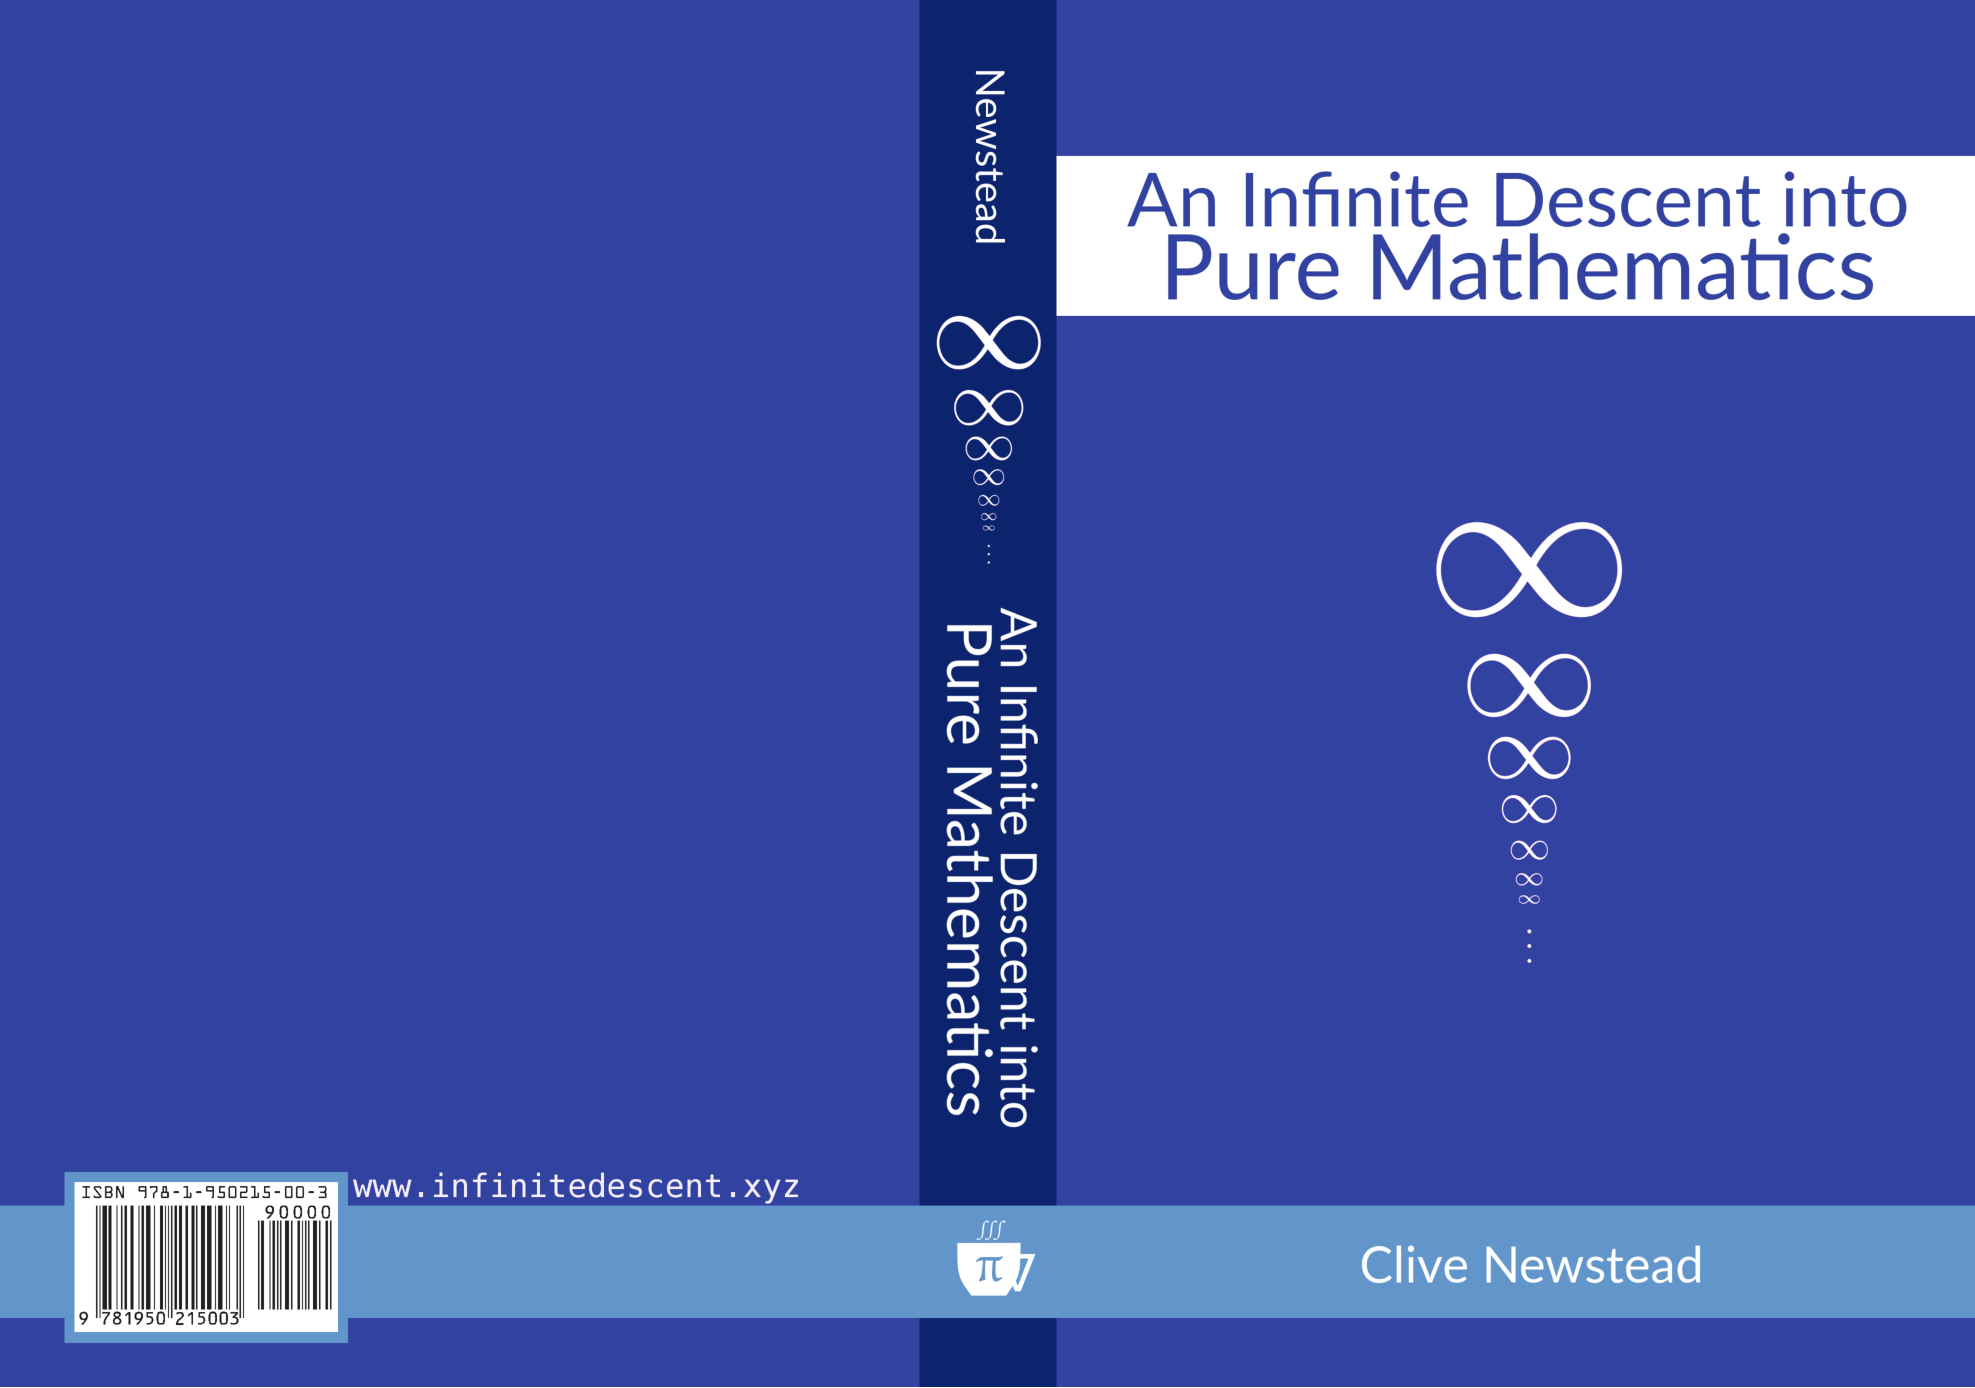
\includepdf[pages=-,fitpaper=true,noautoscale=false]{book/media/spread.pdf}

\frontmatter

% Title page
\newgeometry{centering,bindingoffset={0in}}
% !TeX root = ../../book.tex

$ $

\vfill

\begin{center}
\thispagestyle{empty}

{\Huge \mdseries \fontfamily{bch}\selectfont
An Infinite Descent into\\
Pure Mathematics}

\vfill
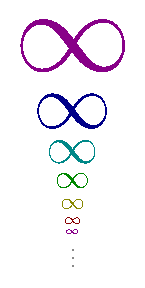
\includegraphics{book/media/logo.pdf}

\vfill


\textsc{by Clive Newstead}\\
\ifadapted{\textit{with adaptations by \adaptername}}

\vfill

\iforiginal{%
\textit{Version \arabic{versionmajor}.\arabic{versionminor}%
\ifnumgreater{\value{versionpatch}}{0}{, revision \arabic{versionpatch}}{}%
\ifnumless{\value{versionpatch}}{0}{ preview}{}}%
\ifnumequal{\value{versionstable}}{0}{ {\color{red}(unstable build)}}{}\\
}
\textit{Last updated on \customdate\today}%
\iforiginal{\\
\url{\bookurl}}
\end{center}
\restoregeometry
\clearpage

% Copyright page
\newpage
{\small
~

\vfill

\thispagestyle{empty}
\ifadaptedelse{%
Original work \textcopyright{} 2019 Clive Newstead, All Rights Reserved.\\
Adaptations \textcopyright{} {\the\year} {\adaptername}, All Rights Reserved.%
}{%
\textcopyright{} 2019 Clive Newstead\\
All Rights Reserved.%
}

\ifadaptedelse{%
Adaptation of Version 
\arabic{versionmajor}.\arabic{versionminor}%
\ifnumgreater{\value{versionpatch}}{0}{.\arabic{versionpatch}}{}%
\ifnumless{\value{versionpatch}}{0}{ (preview)}{}%
}{%
Preview of First Edition, 2019 (forthcoming)
}

ISBN 978-1-950215-00-3 (paperback)\\
ISBN 978-1-950215-01-0 (hardback)

\begin{minipage}{0.75\textwidth}
\small
A free PDF copy of \textit{An Infinite Descent into Pure Mathematics} can be obtained from the book's website:\\
\url{https://infinitedescent.xyz}
\end{minipage}

\begin{minipage}{0.75\textwidth}
\small
This book, its figures and its \TeX{} source are released under a Creative Commons Attribution--ShareAlike 4.0 International Licence. The full text of the licence is replicated at the end of the book, and can be found on the Creative Commons website:\\
\url{https://creativecommons.org/licenses/by/4.0/legalcode}
\end{minipage}

\iforiginal{%
0 ~ 2 ~ 4 ~ 6 ~ 8 ~ 10 ~ 9 ~ 7 ~ 5 ~ 3 ~ 1
}
}

% Table of contents
\bookmark[page=3,level=0]{Contents}
\tableofcontents

% Preface
\chapter*{Preface}
\addcontentsline{toc}{chapter}{Preface}
\markboth{Preface}{Preface}
    Hello, and thank you for taking the time to read this quick introduction to the book! I would like to begin with an apology and a warning:
\begin{center}
\Large \color{red} \bf This book is still under development!
\end{center}
That is to say, there are some sections that are incomplete, as well as other sections which are currently much more terse than I would like them to be.

The most recent version is freely available for download from the following website:
\begin{center}
\url{\bookurl}
\end{center}
As the book is undergoing constant changes, I advise that you do not print it in its entirety---if you must print anything, then I suggest that you do it a few pages at a time, as required.

This book was designed with \textit{inquiry} and \textit{communication} in mind, as they are central to a good mathematical education. One of the upshots of this is that there are many exercises throughout the book, requiring a more active approach to learning, rather than passive reading. These exercises are a fundamental part of the book, and should be completed even if not required by the course instructor. Another upshot of these design principles is that solutions to exercises are not provided---a student seeking feedback on their solutions should speak to someone to get such feedback, be it another student, a teaching assistant or a course instructor.

\subsection*{Navigating the book}

This book need not, and emphatically \textit{should not}, be read from front to back. The order of material is chosen so that material appearing later depends only on material appearing earlier (with a couple of exceptions, which are pointed out in the text).

The majority of introductory pure mathematics courses cover, at a minimum, symbolic logic, sets, functions and relations. This material is the content of \Cref{ptFundamentals}. Such courses usually cover one or more additional topics from pure mathematics, with exactly \textit{which} topics depending on what the course is designing students for. With this in mind, \Cref{ptTopics} serves as an introduction to a range of areas of pure mathematics, including number theory, combinatorics, set theory, real analysis, probability theory and order theory.

It is not necessary to cover all of \Cref{ptFundamentals} before proceeding to topics in \Cref{ptTopics}. In fact, interspersing material from \Cref{ptTopics} can be a useful way of motivating many of the abstract concepts that arise in \Cref{ptFundamentals}.

The following table shows dependencies between sections. Previous sections within the same chapter as a section should be considered `essential' prerequisites unless indicated otherwise.

\begin{center}
\begin{tabular}{c|ccc}
Section & Essential & Recommended & Useful \\ \hline
\ref{secPropositionalLogic} & \ref{chGettingStarted} &  &  \\
\ref{secSets} & \ref{secLogicalEquivalence} &  &  \\
\ref{secPeanosAxioms} & \ref{secLogicalEquivalence} & \ref{secFunctions} & \ref{secInjectionsSurjections} \\
\ref{secRelations} & \ref{secSets} & \ref{secFunctions} & \ref{secInjectionsSurjections}, \ref{secWeakInduction} \\
\ref{secDivision} & \ref{secLogicalEquivalence} & \ref{secSets}, \ref{secStrongInduction} & \ref{secFunctions} \\
\ref{secModularArithmetic} &  & \ref{secEquivalenceRelationsPartitions} &  \\
\ref{secFiniteSets} & \ref{secInjectionsSurjections}, \ref{secStrongInduction} & \ref{secEquivalenceRelationsPartitions} &  \\
\ref{secCountableUncountableSets} & \ref{secFiniteSets} &  &  \\
\ref{secCardinalArithmetic} & \ref{secCountingPrinciples} &  &  \\
\ref{secInequalitiesMeans} & \ref{secPeanosAxioms}, \ref{secSets} &  & \ref{secEquivalenceRelationsPartitions} \\
\ref{secCompletenessConvergence} & \ref{secFunctions} & \ref{secInequalitiesMeans} &  \\
\ref{secSeriesSums} & \ref{secFunctions} & \ref{secInequalitiesMeans} & \ref{secModularArithmetic}, \ref{secCountableUncountableSets} \\
\ref{secDiscreteProbabilitySpaces} & \ref{secCountingPrinciples} & \ref{secCountableUncountableSets}, \ref{secSeriesSums} &  \\
\ref{secOrdersLattices} & \ref{secEquivalenceRelationsPartitions} &  &  \\
\ref{secStructuralInduction} & \ref{secStrongInduction}, \ref{secInjectionsSurjections} & \ref{secCountableUncountableSets} & \ref{secOrdersLattices}
\end{tabular}
\end{center}

Prerequisites are cumulative. For example, in order to cover \Cref{secCardinalArithmetic}, you should first cover \Cref{chGettingStarted,chSetsFunctions,chMathematicalInduction} and \Cref{secFiniteSets,secCountingPrinciples,secCountableUncountableSets,secCardinality}.

\todo{Example courses}

\subsection*{What the numbers, colours and symbols mean}

Broadly speaking, the material in the book is broken down into enumerated items that fall into one of five categories: definitions, results, remarks, examples and exercises. In \Cref{apxWriting}, we also have proof extracts. To improve navigability, these categories are distinguished by name, colour and symbol, as indicated in the following table.

\begin{center}
\begin{tabular}{lcl}
\textbf{Category} & \textbf{Symbol} & \textbf{Colour} \\ \hline
Definitions & \defintrosymbol & {\fontfamily{bch}\color{defcol} \textbf{Red}} \\
Results & \thmintrosymbol & {\fontfamily{bch}\color{thmcol} \textbf{Blue}} \\
Remarks & \tipintrosymbol & {\fontfamily{bch}\color{tipcol} \textbf{Purple}} \\
\end{tabular}
\hspace{20pt}
\begin{tabular}{lcl}
\textbf{Category} & \textbf{Symbol} & \textbf{Colour} \\ \hline
Examples & \exintrosymbol & {\fontfamily{bch}\color{excol} \textbf{Teal}} \\
Exercises & \printrosymbol & {\fontfamily{bch}\color{prcol} \textbf{Gold}} \\
Proof extracts & \quoteintrosymbol & {\fontfamily{bch}\color{excol} \textbf{Teal}}
\end{tabular}
\end{center}
These items are enumerated according to their section---for example, \Cref{thmUniquenessofLimits} is in \Cref{secCompletenessConvergence}. Definitions and theorems (important results) appear in a \fbox{box}.

You will also encounter the symbols $\square$ and \nonproofqedsymbol{} whose meanings are as follows:

\begin{itemize}
\item[$\square$] \textbf{End of proof.} It is standard in mathematical documents to identify when a proof has ended by drawing a small square or by writing `\textit{Q.E.D.}' (The latter stands for \textit{quod erat demonstrandum}, which is Latin for \textit{which was to be shown}.)
\item[\nonproofqedsymbol] \textbf{End of item.} This is \textit{not} a standard usage, and is included only to help you to identify when an item has finished and the main content of the book continues.
\end{itemize}

Some subsections are labelled with the symbol \optmarksymbol{}. This indicates that the material in that subsection can be skipped without dire consequences.

\subsection*{Licence}

This book is licensed under the Creative Commons Attribution-ShareAlike 4.0 (\textsc{cc by-sa 4.0}) licence. This means you're welcome to share this book, provided that you give credit to the author and that any copies or derivatives of this book are released under the same licence. The content of the licence can be read in its full glory at the end of the book, and by following the following URL:
\begin{center}
\url{http://creativecommons.org/licenses/by-sa/4.0/}
\end{center}

\subsection*{Comments and corrections}

Any feedback, be it from students, teaching assistants, instructors or any other readers, would be very much appreciated. Particularly useful are corrections of typographical errors, suggestions for alternative ways to describe concepts or prove theorems, and requests for new content (e.g.\ if you know of a nice example that illustrates a concept, or if there is a relevant concept you wish were included in the book).

Such feedback can be sent to the author by email (\url{\authoremail}).

% Acknowledgements
\chapter*{Acknowledgements}
\addcontentsline{toc}{chapter}{Acknowledgements}
\markboth{Acknowledgements}{Acknowledgements}
    % !TeX root = ../../book.tex
\chapter*{Acknowledgements}
\addcontentsline{toc}{chapter}{Acknowledgements}
\markboth{Acknowledgements}{Acknowledgements}

When I reflect on the time I have spent writing this book, I am overwhelmed by the number of people who have had some kind of influence on its content.

This book would never have come to exist were it not for Chad Hershock's course 38-801 \textit{Evidence-Based Teaching in the Sciences}, which I took in Fall 2014 as a graduate student at Carnegie Mellon University. His course heavily influenced my approach to teaching, and it motivated me to write this book in the first place. Many of the pedagogical decisions I made when writing this book were informed by research that I was exposed to as a student in Chad's class.

The legendary Carnegie Mellon professor, John Mackey, has been using this book (in various forms) as course notes for 21-128 \textit{Mathematical Concepts and Proofs} and 15-151 \textit{Mathematical Foundations of Computer Science} since Fall 2016. His influence can be felt throughout the book: thanks to discussions with John, many proofs have been reworded, sections restructured, and explanations improved. As a result, there is some overlap between the exercises in this book and the questions on his problem sheets. I am extremely grateful for his ongoing support.

Steve Awodey, who was my doctoral thesis advisor, has for a long time been a source of inspiration for me. Many of the choices I made when choosing how to present the material in this book are grounded in my desire to do mathematics \textit{the right way}---it was this desire that led me to study category theory, and ultimately to become Steve's PhD student. I learnt a great deal from him and I greatly appreciated his patience and flexibility in helping direct my research despite my busy teaching schedule and extracurricular interests (such as writing this book).

Perhaps unbeknownst to them, many insightful conversations with the following people have helped shape the material in this book in one way or another: Jeremy Avigad, Deb Brandon, Santiago Ca\~{n}ez, Heather Dwyer, Thomas Forster, Will Gunther, Kate Hamilton, Jessica Harrell, Bob Harper, Brian Kell, Marsha Lovett, Ben Millwood, David Offner, Ruth Poproski, Emily Riehl, Hilary Schuldt, Gareth Taylor, Katie Walsh, Emily Weiss and Andy Zucker.

The \textit{Stack Exchange} network has influenced the development of this book in two important ways. First, I have been an active member of \textit{Mathematics Stack Exchange} (\url{https://math.stackexchange.com/}) since early 2012 and have learnt a great deal about how to effectively explain mathematical concepts; occasionally, a question on Mathematics Stack Exchange inspires me to add a new example or exercise to the book. Second, I have made frequent use of \textit{\LaTeX{} Stack Exchange} (\url{https://tex.stackexchange.com}) for implementing some of the more technical aspects of writing a book using \LaTeX{}.

The Department of Mathematical Sciences at Carnegie Mellon University supported me academically, professionally and financially throughout my PhD and presented me with more opportunities than I could possibly have hoped for to develop as a teacher. This support is now continued by the Department of Mathematics at Northwestern University, where I am currently employed as a lecturer.

I would also like to thank everyone at Carnegie Mellon's and Northwestern's teaching centres, the Eberly Center and the Searle Center, respectively. Through various workshops, programs and fellowships at both teaching centres, I have learnt an incredible amount about how people learn, and I have transformed as a teacher. Their student-centred, evidence-based approach to the science of teaching and learning underlies everything I do as a teacher, including writing this book---their influence cannot be understated.

Finally, and importantly, I am grateful to the 1000+ students who have already used this book to learn mathematics. Every time a student contacts me to ask a question or point out an error, the book gets better; this is reflected in the dozens of typographical errors that have been fixed as a consequence.

\begin{flushright}
Clive Newstead\\
January 2020\\
Evanston, Illinois
\end{flushright}

\mainmatter

\setcounter{chapter}{-1}

\chapter{Getting started}
\markboth{Chapter \thechapter.\ Getting started}{Chapter \thechapter.\ Getting started}
    \label{chGettingStarted}
    \chapter{Getting started}
\markboth{Chapter \thechapter.\ Getting started}{Chapter \thechapter.\ Getting started}
\label{chGettingStarted}

\renewcommand{\currentchapter}{00}

\numberitemswithin{chapter}

\hintsection{\Cref*{chGettingStarted}}

Before we can start proving things, we need to eliminate certain kinds of statements that we might try to prove. Consider the following statement:
\begin{center} \textit{This sentence is false.} \end{center}
Is it true or false? If you think about this for a couple of seconds then you'll get into a bit of a pickle.

Now consider the following statement:
\begin{center} \textit{The happiest donkey in the world.} \end{center}
Is it true or false? Well it's not even a sentence; it doesn't make sense to even \textit{ask} if it's true or false!

Clearly we'll be wasting our time trying to write proofs of statements like the two listed above---we need to narrow our scope to statements that we might actually have a chance of proving (or perhaps refuting)! This motivates the following (informal) definition.

\begin{definition}
\label{defProposition}
\label{defProof}
\index{proposition}
\index{proof}
A \textbf{proposition} \index{proposition} is a statement to which it is possible to assign a \textbf{truth value} (`true' or `false'). If a proposition is true, a \textbf{proof} of the proposition is a logically valid argument demonstrating that it is true, which is pitched at such a level that a member of the intended audience can verify its correctness.
\end{definition}

Thus the statements given above are not propositions because there is no possible way of assigning them a truth value. Note that, in \Cref{defProposition}, all that matters is that it \textit{makes sense} to say that it is true or false, regardless of whether it actually \textit{is} true or false---the truth value of many propositions is unknown, even very simple ones.

\begin{exercise}
Think of an example of a true proposition, a false proposition, a proposition whose truth value you don't know, and a statement that is not a proposition.
\end{exercise}

Results in mathematical papers and textbooks may be referred to as \textit{propositions}, but they may also be referred to as \textit{theorems}, \textit{lemmas} or \textit{corollaries} depending on their intended usage.
\begin{itemize} 
\item A \textbf{proposition} is an umbrella term which can be used for any result.
\item A \textbf{theorem} is a key result which is particularly important.
\item A \textbf{lemma} is a result which is proved for the purposes of being used in the proof of a theorem. 
\item A \textbf{corollary} is a result which follows from a theorem without much additional effort.
\end{itemize}
These are not precise definitions, and they are not meant to be---you could call every result a \textit{proposition} if you wanted to---but using these words appropriately helps readers work out how to read a paper. For example, if you just want to skim a paper and find its key results, you'd look for results labelled as \textit{theorems}.

It is not much good trying to prove results if we don't have anything to prove results about. With this in mind, we will now introduce the \textit{number sets} and prove some results about them in the context of four topics, namely: division of integers, number bases, rational and irrational numbers, and polynomials. These topics will provide context for the material in \Cref{ptCoreConcepts}, and serve as an introduction to the topics covered in \Cref{ptTopics}.

We will not go into very much depth in this chapter. Rather, think of this as a warm-up exercise---a quick, light introduction, with more proofs to be provided in the rest of the book.

\subsection*{Number sets}

Later in this chapter, and then in much more detail in \Cref{chSets}, we will encounter the notion of a \textit{set}; a set can be thought of as being a collection of objects. This seemingly simple notion is fundamental to mathematics, and is so involved that we will not treat sets formally in this book. For now, the following definition will suffice.

\begin{definition}[to be revised in \Cref{defSet}]
\label{defSetsPreliminary}
\lindexmmc{in}{$\in$}
A \textbf{set} is a collection of objects. The objects in the set are called \textbf{elements} of the set. If $X$ is a set and $x$ is an object, then we write $x \in X$ \inlatexnb{x \textbackslash{}in X} to denote the assertion that $x$ is an element of $X$.
\end{definition}

The sets of concern to us first and foremost are the \textit{number sets}---that is, sets whose elements are particular types of \textit{number}. At this introductory level, many details will be temporarily swept under the rug; we will work at a level of precision which is appropriate for our current stage, but still allows us to develop a reasonable amount of intuition.

In order to define the number sets, we will need three things: an infinite line, a fixed point on this line, and a fixed unit of length.

So here we go. Here is an infinite line:
\begin{center}
\begin{tikzpicture}
\draw[latex-latex] (-5.5, 0) -- (5.5, 0) ;
\end{tikzpicture}
\end{center}
The arrows indicate that it is supposed to extend in both directions without end. The points on the line will represent numbers (specifically, \textit{real numbers}, a misleading term that will be defined in \Cref{defRealsInformal}). Now let's fix a point on this line, and label it `$0$':
\begin{center}
\begin{tikzpicture}
\draw[latex-latex] (-5.5, 0) -- (5.5, 0) ; 
\draw (0, 0) -- (0, 0.1) node[above] {$0$} ;
\end{tikzpicture}
\end{center}
This point can be thought of as representing the number zero; it is the point against which all other numbers will be measured. Finally, let's fix a unit of length:
\begin{center}
\begin{tikzpicture}
\draw (0, 0) -- (1, 0) ; 
\foreach \x in {0,1} \draw (\x, -0.1) -- (\x, 0.1)  ;
\end{tikzpicture}
\end{center}
This unit of length will be used, amongst other things, to compare the extent to which the other numbers differ from zero.

\begin{definition}
\label{defNumberLine}
The above infinite line, together with its fixed zero point and fixed unit length, constitute the (\textbf{real}) \textbf{number line}.
\end{definition}

We will use the number line to construct five sets of numbers of interest to us:
\begin{itemize}
\item The set $\mathbb{N}$ of \textit{natural numbers}---\Cref{defNaturalNumbersInformal};
\item The set $\mathbb{Z}$ of \textit{integers}---\Cref{defIntegersInformal};
\item The set $\mathbb{Q}$ of \textit{rational numbers}---\Cref{defRationalsInformal};
\item The set $\mathbb{R}$ of \textit{real numbers}---\Cref{defRealsInformal}; and
\item The set $\mathbb{C}$ of \textit{complex numbers}---\Cref{defComplexNumbersInformal}.
\end{itemize}

Each of these sets has a different character and is used for different purposes, as we will see both later in this chapter and throughout this book.

\subsection*{Natural numbers ($\mathbb{N}$)}

The \textit{natural numbers} are the numbers used for counting---they are the answers to questions of the form `how many'---for example, I have \textit{three} uncles, \textit{one} dog and \textit{zero} cats.

Counting is a skill humans have had for a very long time; we know this because there is evidence of people using tally marks tens of thousands of years ago. Tally marks provide one method of counting small numbers: starting with nothing, proceed through the objects you want to count one by one, and make a mark for every object. When you are finished, there will be as many marks as there are objects. We are taught from a young age to count with our fingers; this is another instance of making tally marks, where now instead of making a mark we raise a finger.

Making a tally mark represents an \textit{increment} in quantity---that is, adding one. On our number line, we can represent an increment in quantity by moving to the right by the unit length. Then the distance from zero we have moved, which is equal to the number of times we moved right by the unit length, is therefore equal to the number of objects being counted.

\begin{definition}
\label{defNaturalNumbersInformal}
The \textbf{natural numbers} are represented by the points on the number line which can be obtained by starting at $0$ and moving right by the unit length any number of times:
\begin{center}
\begin{tikzpicture}
\draw[latex-latex] (-5.5, 0) -- (5.5, 0) ; 
\foreach \x in {0,1,2,3,4,5} \draw (\x, 0) -- (\x, 0.1) node[above] {$\x$} ;
\end{tikzpicture}
\end{center}
In more familiar terms, they are the \textit{non-negative whole numbers}. We write $\mathbb{N}$ \inlatex{mathbb\{N\}}\lindexmmc{mathbb}{$\mathbb{A}, \mathbb{B}, \dots$} for the set of all natural numbers; thus, the notation `$n \in \mathbb{N}$' means that $n$ is a natural number.
\end{definition}

The natural numbers have very important and interesting mathematical structure, and are central to the material in \Cref{chCombinatorics}. A more precise characterisation of the natural numbers will be provided in \Cref{secPeanosAxioms}, and a mathematical construction of the set of natural numbers can be found in \Cref{secZFC} (see \Cref{cnsNaturalNumbersVonNeumann}). Central to these more precise characterisations will be the notions of `zero' and of `adding one'---just like making tally marks.

\begin{aside}
Some authors define the natural numbers to be the \textit{positive} whole numbers, thus excluding zero. We take $0$ to be a natural number since our main use of the natural numbers will be for counting finite sets, and a set with nothing in it is certainly finite! That said, as with any mathematical definition, the choice about whether $0 \in \mathbb{N}$ or $0 \not \in \mathbb{N}$ is a matter of taste or convenience, and is merely a convention---it is not something that can be proved or refuted.
\end{aside}

\subsection*{Number bases}

Writing numbers down is something that may seem easy to you now, but it likely took you several years as a child to truly understand what was going on. Historically, there have been many different systems for representing numbers symbolically, called \textit{numeral systems}.\index{numeral system} First came the most primitive of all, tally marks, appearing in the Stone Age and still being used for some purposes today. Thousands of years and hundreds of numeral systems later, there is one dominant numeral system, understood throughout the world: the \textbf{Hindu--Arabic numeral system}.\index{numeral system!Hindu--Arabic} This numeral system consists of ten symbols, called \textit{digits}. It is a \textit{positional} numeral system, meaning that the position of a symbol in a string determines its numerical value.

In English, the \textit{Arabic numerals} are used as the ten digits:
\[ 0 \quad 1 \quad 2 \quad 3 \quad 4 \quad 5 \quad 6 \quad 7 \quad 8 \quad 9 \]
The right-most digit in a string is in the units place, and the value of each digit increases by a factor of ten moving to the left. For example, when we write `$2812$', the left-most `$2$' represents the number two thousand, whereas the last `$2$' represents the number two.

The fact that there are ten digits, and that the numeral system is based on powers of ten, is a biological accident corresponding with the fact that most humans have ten fingers. For many purposes, this is inconvenient. For example, ten does not have many positive divisors (only four)---this has implications for the ease of performing arithmetic; a system based on the number twelve, which has six positive divisors, might be more convenient. Another example is in computing and digital electronics, where it is more convenient to work in a \textit{binary} system, with just two digits, which represent `off' and `on' (or `low voltage' and `high voltage'), respectively; arithmetic can then be performed directly using sequences of \textit{logic gates} in an electrical circuit.

It is therefore worthwhile to have some understanding of positional numeral systems based on numbers other than ten. The mathematical abstraction we make leads to the definition of \textit{base-$b$ expansion}.

\begin{definition}
\label{defBaseBExpansionPreliminary}
\index{base-$b$ expansion}
\index{number base}
Let $b>1$. The \textbf{base-$b$ expansion} of a natural number $n$ is the\footnote{The use of the word `the' is troublesome here, since it assumes that every natural number has only one base-$b$ expansion. This fact actually requires proof---see \Cref{thmBaseBExpansion}.} string $d_r d_{r-1} \dots d_0$ such that
\begin{itemize}
\item $n = d_r \cdot b^r + d_{r-1} \cdot b^{r-1} + \cdots + d_0 \cdot b^0$;
\item $0 \le d_i < b$ for each $i$; and
\item If $n>0$ then $d_r \ne 0$---the base-$b$ expansion of zero is $0$ in all bases $b$.
\end{itemize}
Certain number bases have names; for instance, the base-$2$, $3$, $8$, $10$ and $16$ expansions are respectively called \textit{binary}, \textit{ternary}, \textit{octal}, \textit{decimal} and \textit{hexadecimal}.
\end{definition}

\begin{example}
Consider the number $1023$. Its decimal (base-$10$) expansion is $1023$, since
\[ 1023 = 1 \cdot 10^3 + 0 \cdot 10^2 + 2 \cdot 10^1 + 3 \cdot 10^0 \]
Its binary (base-$2$) expansion is $1111111111$, since
\[ 1023 = 1 \cdot 2^9 + 1 \cdot 2^8 + 1 \cdot 2^7 + 1 \cdot 2^6 + 1 \cdot 2^5 + 1 \cdot 2^4 + 1 \cdot 2^3 + 1 \cdot 2^2 + 1 \cdot 2^1 + 1 \cdot 2^0 \]
We can express numbers in base-$36$ by using the ten usual digits $0$ through $9$ and the twenty-six letters $\mathrm{A}$ through $\mathrm{Z}$; for instance, $\mathrm{A}$ represents $10$, $\mathrm{M}$ represents $22$ and $\mathrm{Z}$ represents $35$. The base-$36$ expansion of $1023$ is $\mathrm{SF}$, since
\[ 1023 = 28 \cdot 36^1 + 15 \cdot 36^0 = \mathrm{S} \cdot 36^1 + \mathrm{F} \cdot 36^0 \]
\end{example}

\begin{exercise}
Find the binary, ternary, octal, decimal, hexadecimal and base-$36$ expansions of the number $21127$, using the letters $\mathrm{A}$--$\mathrm{F}$ as additional digits for the hexadecimal expansion and the letters $\mathrm{A}$--$\mathrm{Z}$ as additional digits for the base-$36$ expansion.
\end{exercise}

We sometimes wish to specify a natural number in terms of its base-$b$ expansion; we have some notation for this.

\begin{notation}
Let $b>1$. If the numbers $d_0,d_1,\dots,d_r$ are base-$b$ digits (in the sense of \Cref{defBaseBExpansionPreliminary}), then we write
\[ {d_rd_{r-1} \dots d_0}_{(b)} = d_r \cdot b^r + d_{r-1} \cdot b^{r-1} + \cdots + d_0 \cdot b^0 \]
for the natural number whose base-$b$ expansion is $d_rd_{r-1} \dots d_0$. If there is no subscript $(b)$ and a base is not specified explicitly, the expansion will be assumed to be in base-$10$.
\end{notation}

\begin{example}
Using our new notation, we have
\[ 1023 = 1111111111_{(2)} = 1101220_{(3)} = 1777_{(8)} = 1023_{(10)} = 3\mathrm{FF}_{(16)} = \mathrm{SF}_{(36)} \]
\end{example}

\subsection*{Integers ($\mathbb{Z}$)}

The \textit{integers} can be used for measuring the difference between two instances of counting. For example, suppose I have five apples and five bananas. Another person, also holding apples and bananas, wishes to trade. After our exchange, I have seven apples and only one banana. Thus I have two more apples and four fewer bananas.

Since an increment in quantity can be represented by moving to the right on the number line by the unit length, a \textit{decrement} in quantity can therefore be represented by moving to the \textit{left} by the unit length. Doing so gives rise to the integers.

\begin{definition}
\label{defIntegersInformal}
The \textbf{integers} are represented by the points on the number line which can be obtained by starting at $0$ and moving in either direction by the unit length any number of times:
\begin{center}
\begin{tikzpicture}
\draw[latex-latex] (-5.5, 0) -- (5.5, 0) ; 
\foreach \x in {-5,-4,-3,-2,-1,0,1,2,3,4,5} \draw (\x, 0) -- (\x, 0.1) node[above] {$\x$} ;
\end{tikzpicture}
\end{center}
We write $\mathbb{Z}$ \inlatex{mathbb\{Z\}}\lindexmmc{mathbb}{$\mathbb{A}, \mathbb{B}, \dots$} for the set of all integers; thus, the notation `$n \in \mathbb{Z}$' means that $n$ is an integer.
\end{definition}

The integers have such a fascinating structure that a whole chapter of this book is devoted to them---see \Cref{chNumberTheory}. This is to do with the fact that, although you can add, subtract and multiply two integers and obtain another integer, the same is not true of division. This `bad behaviour' of division is what makes the integers interesting. We will now see some basic results about division.

\subsection*{Division of integers}
\label{pGettingStartedDivision}

The motivation we will soon give for the definition of the rational numbers (\Cref{defRationalsInformal}) is that the result of dividing one integer by another integer is not necessarily another integer. However, the result is \textit{sometimes} another integer; for example, I can divide six apples between three people, and each person will receive an integral number of apples. This makes division interesting: how can we measure the failure of one integer's divisibility by another? How can we deduce when one integer is divisible by another? What is the structure of the set of integers when viewed through the lens of division? This motivates \Cref{defDivisionPreliminary}.

\begin{definition}[to be repeated in \Cref{defDivision}]
\label{defDivisionPreliminary}
\index{division}
\index{divisor}
\index{factor}
\index{multiple}
Let $a,b \in \mathbb{Z}$. We say $b$ \textbf{divides} $a$ if $a=qb$ for some integer $q$. Other ways of saying that $b$ divides $a$ are: $b$ is a \textit{divisor} of $a$, $b$ is a \textit{factor} of $a$, or $a$ is a \textit{multiple} of $b$.
\end{definition}

\begin{example}
The integer $12$ is divisible by $1$, $2$, $3$, $4$, $6$ and $12$, since
\[ 12 = 12 \cdot 1 = 6 \cdot 2 = 4 \cdot 3 = 3 \cdot 4 = 2 \cdot 6 = 1 \cdot 12 \]
It is also divisible by the negatives of all of those numbers; for example, $12$ is divisible by $-3$ since $12 = (-4) \cdot (-3)$.
\end{example}

\begin{exercise}
Prove that $1$ divides every integer, and that every integer divides $0$.
\end{exercise}

Using \Cref{defDivisionPreliminary}, we can prove some general basic facts about divisibility.

\begin{proposition}
\label{propDivisibilityIsTransitive}
Let $a,b,c \in \mathbb{Z}$. If $c$ divides $b$ and $b$ divides $a$, then $c$ divides $a$.
\end{proposition}

\begin{cproof}
Suppose that $c$ divides $b$ and $b$ divides $a$. By \Cref{defDivisionPreliminary}, it follows that
\[ b=qc \quad \text{and} \quad a=rb \]
for some integers $q$ and $r$. Using the first equation, we may substitute $qc$ for $b$ in the second equation, to obtain
\[ a=r(qc) \]
But $r(qc) = (rq)c$, and $rq$ is an integer, so it follows from \Cref{defDivisionPreliminary} that $c$ divides $a$.
\end{cproof}

% To do: draw attention to the wording of the proof, and the 'unpack definition - do something - apply definition' style of the proof.

\begin{exercise}
\label{exDivisibilityIsLinear}
Let $a,b,d \in \mathbb{Z}$. Suppose that $d$ divides $a$ and $d$ divides $b$. Given integers $u$ and $v$, prove that $d$ divides $au+bv$.
\end{exercise}

Some familiar concepts, such as evenness and oddness, can be characterised in terms of divisibility.

\begin{definition}
\label{defEvenOdd}
\index{even!integer}
\index{odd!integer}
An integer $n$ is \textbf{even} if it is divisible by $2$; otherwise, $n$ is \textbf{odd}.
\end{definition}

It is not just interesting to know when one integer \textit{does} divide another; however, proving that one integer \textit{doesn't} divide another is much harder. Indeed, to prove that an integer $b$ does not divide an integer $a$, we must prove that $a \ne qb$ for \textit{any} integer $q$ at all. We will look at methods for doing this in \Cref{chLogicalStructure}; these methods use the following extremely important result, which will underlie all of \Cref{chNumberTheory}.

\begin{theorem}[Division theorem, to be repeated in \Cref{thmDivisionTheorem}]
\label{thmDivisionPreliminary}
\index{division theorem}
Let $a,b \in \mathbb{Z}$ with $b \ne 0$. There is exactly one way to write
\[ a = qb + r \]
such that $q$ and $r$ are integers, and $0 \le r < b$ (if $b > 0$) or $0 \le r < -b$ (if $b < 0$).
\end{theorem}

The number $q$ in \Cref{thmDivisionPreliminary} is called the \textbf{quotient}\index{quotient} of $a$ when divided by $b$, and the number $r$ is called the \textbf{remainder}\index{remainder}.

\begin{example}
The number $12$ leaves a remainder of $2$ when divided by $5$, since $12 = 2 \cdot 5 + 2$.
\end{example}

Here's a slightly more involved example.

\begin{proposition}
Suppose an integer $a$ leaves a remainder of $r$ when divided by an integer $b$, and that $r>0$. Then $-a$ leaves a remainder of $b-r$ when divided by $b$.
\end{proposition}

\begin{cproof}
Suppose $a$ leaves a remainder of $r$ when divided by $b$. Then
\[ a=qb+r \]
for some integer $q$. A bit of algebra yields
\[ -a = -qb-r = -qb-r+(b-b) = -(q+1)b + (b-r) \]
Since $0<r<b$, we have $0<b-r<b$. Hence $-(q+1)$ is the quotient of $-a$ when divided by $b$, and $b-r$ is the remainder.
\end{cproof}

\begin{exercise}
Prove that if an integer $a$ leaves a remainder of $r$ when divided by an integer $b$, then $a$ leaves a remainder of $r$ when divided by $-b$.
\end{exercise}

We will finish this part on division of integers by connecting it with the material on number bases---we can use the division theorem (\Cref{thmDivisionPreliminary}) to find the base-$b$ expansion of a given natural number. It is based on the following observation: the natural number $n$ whose base-$b$ expansion is $d_rd_{r-1} \cdots d_1 d_0$ is equal to
\[ d_0 + b(d_1 + b(d_2 + \cdots + b(d_{r-1} + bd_r) \cdots)) \]
Moreover, $0 \le d_i < b$ for all $i$. In particular $n$ leaves a remainder of $d_0$ when divided by $b$. Hence
\[ \frac{n-d_0}{b} = d_1 + d_2b + \cdots + d_rb^{r-1} \]
The base-$b$ expansion of $\frac{n-d_0}{b}$ is therefore
\[ d_rd_{r-1} \cdots d_1 \]
In other words, the remainder of $n$ when divided by $b$ is the last base-$b$ digit of $n$, and then subtracting this number from $n$ and dividing the result by $b$ truncates the final digit. Repeating this process gives us $d_1$, and then $d_2$, and so on, until we end up with $0$.

This suggests the following algorithm for computing the base-$b$ expansion of a number $n$:
\begin{itemize}
\item \textbf{Step 1.} Let $d_0$ be the remainder when $n$ is divided by $b$, and let $n_0=\frac{n-d_0}{b}$ be the quotient. Fix $i=0$.
\item \textbf{Step 2.} Suppose $n_i$ and $d_i$ have been defined. If $n_i=0$, then proceed to Step 3. Otherwise, define $d_{i+1}$ to be the remainder when $n_i$ is divided by $b$, and define $n_{i+1} = \frac{n_i-d_{i+1}}{b}$. Increment $i$, and repeat Step 2.
\item \textbf{Step 3.} The base-$b$ expansion of $n$, is
\[ d_id_{i-1} \cdots d_0 \]
\end{itemize}

\begin{example}
We compute the base-$17$ expansion of $15213$, using the letters $\mathrm{A}$--$\mathrm{G}$ to represent the numbers $10$ through $16$.
\begin{itemize}
\item $15213 = 894 \cdot 17 + 15$, so $d_0=15=\mathrm{F}$ and $n_0=894$.
\item $894 = 52 \cdot 17 + 10$, so $d_1=10 = \mathrm{A}$ and $n_1=52$.
\item $52 = 3 \cdot 17 + 1$, so $d_2 = 1$ and $n_2=3$.
\item $3 = 0 \cdot 17 + 3$, so $d_3 = 3$ and $n_3=0$.
\item The base-$17$ expansion of $15213$ is therefore $31\mathrm{AF}$.
\end{itemize}
A quick verification gives
\[ 31\mathrm{AF}_{(17)} = 3 \cdot 17^3 + 1 \cdot 17^2 + 10 \cdot 17 + 15 = 15213 \]
as desired.
\end{example}

\begin{exercise}
Find the base-$17$ expansion of $408\,735\,787$ and the base-$36$ expansion of $1\,442\,151\,747$.
\end{exercise}

\subsection*{Rational numbers ($\mathbb{Q}$)}

Bored of eating apples and bananas, I buy a pizza which is divided into eight slices. A friend and I decide to share the pizza. I don't have much of an appetite, so I eat three slices and my friend eats five. Unfortunately, we cannot represent the proportion of the pizza each of us has eaten using natural numbers or integers. However, we're not far off: we can count the number of equal parts the pizza was split into, and of those parts, we can count how many we had. On the number line, this could be represented by splitting the unit line segment from $0$ to $1$ into eight equal pieces, and proceeding from there. This kind of procedure gives rise to the \textit{rational numbers}.

\begin{definition}
\label{defRationalsInformal}
The \textbf{rational numbers} are represented by the points at the number line which can be obtained by dividing any of the unit line segments between integers into an equal number of parts.
\begin{center}
\begin{tikzpicture}
\draw[latex-latex] (-5.5, 0) -- (5.5, 0) ; 
\foreach \x in {-5,-4,-3,-2,-1,0,1,2,3,4,5} \draw (\x, 0) -- (\x, 0.25) node[above] {$\x$} ;
\foreach \x in {-5,-4,-3,-2,-1,0,1,2,3,4,5} {
  \foreach \i in {-0.33,0.33} {
    \draw (\x+\i, 0) -- (\x+\i, 0.15) ;
  }
}
\end{tikzpicture}
\end{center}
The rational numbers are those of the form $\frac{a}{b}$, where $a,b \in \mathbb{Z}$ and $b \ne 0$. We write $\mathbb{Q}$ \inlatex{mathbb\{Q\}}\lindexmmc{mathbb}{$\mathbb{A}, \mathbb{B}, \dots$} for the set of all rational numbers; thus, the notation `$q \in \mathbb{Q}$' means that $q$ is a rational number.
\end{definition}

The rational numbers are a very important example of a type of algebraic structure known as a \textit{field}---they are particularly central to algebraic number theory and algebraic geometry.

\subsection*{Real numbers ($\mathbb{R}$)}

Quantity and change can be measured in the abstract using \textit{real numbers}.

\begin{definition}
\label{defRealsInformal}
The \textbf{real numbers} are the points on the number line. We write $\mathbb{R}$ \inlatex{mathbb\{R\}}\lindexmmc{mathbb}{$\mathbb{A}, \mathbb{B}, \dots$} for the set of all real numbers; thus, the notation `$a \in \mathbb{R}$' means that $a$ is a real number.
\end{definition}

The real numbers are central to real analysis, a branch of mathematics introduced in \Cref{chRealNumbers}. They turn the rationals into a \textit{continuum} by `filling in the gaps'---specifically, they have the property of \textit{completeness}, meaning that if a quantity can be approximated with arbitrary precision by real numbers, then that quantity is itself a real number.

We can define the basic arithmetic operations (addition, subtraction, multiplication and division) on the real numbers, and a notion of ordering of the real numbers, in terms of the infinite number line.

\begin{itemize}
\item \textbf{Ordering.} A real number $a$ is less than a real number $b$, written $a<b$, if $a$ lies to the left of $b$ on the number line. The usual conventions for the symbols $\le$ \inlatex{le}\lindexmmc{le}{$\le$}, $>$ and $\ge$ \inlatex{ge}\lindexmmc{ge}{$\ge$} apply, for instance `$a \le b$' means that either $a < b$ or $a = b$.

\item \textbf{Addition.} Suppose we want to add a real number $a$ to a real number $b$. To do this, we \textit{translate} $a$ by $b$ units to the right---if $b<0$ then this amounts to translating $a$ by an equivalent number of units to the left. Concretely, take two copies of the number line, one above the other, with the same choice of unit length; move the $0$ of the lower number line beneath the point $a$ of the upper number line. Then $a+b$ is the point on the upper number line lying above the point $b$ of the lower number line.

Here is an illustration of the fact that $(-3) + 5 = 2$:

\begin{center}
\fitwidthc{0.9}{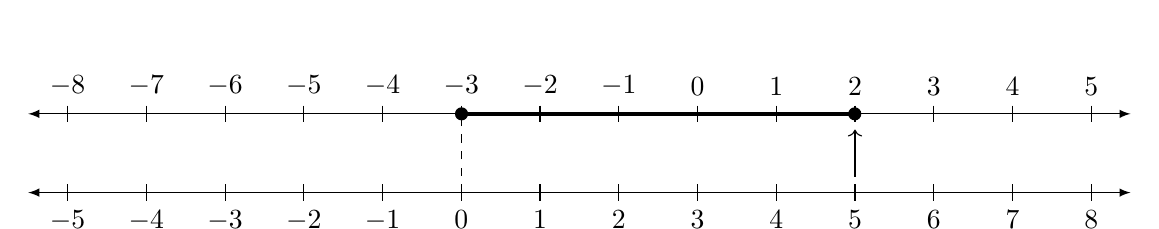
\begin{tikzpicture}
% Adapted from http://tex.stackexchange.com/questions/148252/
\draw[latex-latex] (-8.5,0) -- (5.5,0) ; 
\foreach \x in  {-8,-7,-6,-5,-4,-3,-2,-1,0,1,2,3,4,5}
\draw[shift={(\x,0)}] (0pt,3pt) -- (0pt,-3pt);
\foreach \x in {-8,-7,-6,-5,-4,-3,-2,-1,0,1,2,3,4,5}
\draw[shift={(\x,0)}] (0pt,0pt) -- (0pt,3pt) node[above] {$\x$};
\draw[*-*] (-3.08,0) -- (2.08,0);
\draw[very thick] (-3,0) -- (2,0);

\draw[latex-latex] (-8.5,-1) -- (5.5,-1) ; 
\foreach \x in  {-5,-4,-3,-2,-1,0,1,2,3,4,5,6,7,8}
\draw[shift={(\x-3,-1)},color=black] (0pt,3pt) -- (0pt,-3pt);
\foreach \x in {-5,-4,-3,-2,-1,0,1,2,3,4,5,6,7,8}
\draw[shift={(\x-3,-1)},color=black] (0pt,0pt) -- (0pt,-3pt) node[below] {$\x$};
\draw[dashed] (-3,-1) -- (-3,0) ;
\draw[->] (2,-0.8) -- (2,-0.2) ;
\end{tikzpicture}}
\end{center}

\item \textbf{Multiplication.} This one is fun. Suppose we want to multiply a real number $a$ by a real number $b$. To do this, we \textit{scale} the number line, and perhaps \textit{reflect} it. Concretely, take two copies of the number line, one above the other; align the $0$ points on both number lines, and stretch the lower number line evenly until the point $1$ on the lower number line is below the point $a$ on the upper number line---note that if $a<0$ then the number line must be reflected in order for this to happen. Then $a \cdot b$ is the point on the upper number line lying above $b$ on the lower number line.

Here is an illustration of the fact that $5 \cdot 4 = 20$.

\begin{center}
\fitwidthc{0.9}{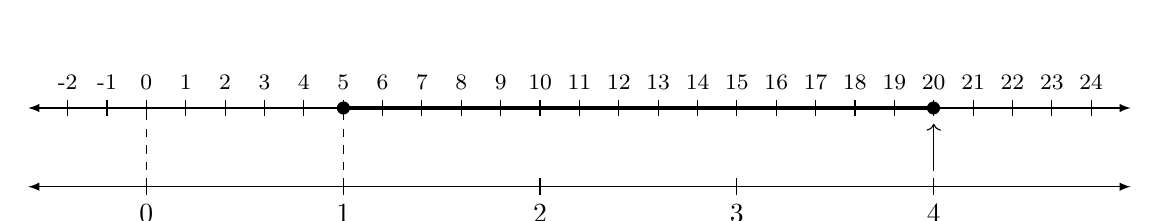
\begin{tikzpicture}
% Adapted from http://tex.stackexchange.com/questions/148252/
\draw[latex-latex] (-5.5,0) -- (8.5,0) ; 
\foreach \x in  {-2,-1,0,1,2,3,4,5,6,7,8,9,10,11,12,13,14,15,16,17,18,19,20,21,22,23,24}
\draw[shift={(0.5*\x-4,0)}] (0pt,3pt) -- (0pt,-3pt);
\foreach \x in {-2,-1,0,1,2,3,4,5,6,7,8,9,10,11,12,13,14,15,16,17,18,19,20,21,22,23,24}
\draw[shift={(0.5*\x-4,0)}] (0pt,0pt) -- (0pt,3pt) node[above] {$\text{\footnotesize\x}$};
\draw[*-*] (-1.58,0) -- (6.08,0);
\draw[very thick] (-1.5,0) -- (6,0);

\draw[latex-latex] (-5.5,-1) -- (8.5,-1) ; 
\foreach \x in  {0,1,2,3,4}
\draw[shift={(2.5*\x-4,-1)},color=black] (0pt,3pt) -- (0pt,-3pt);
\foreach \x in {0,1,2,3,4}
\draw[shift={(2.5*\x-4,-1)},color=black] (0pt,0pt) -- (0pt,-3pt) node[below] {$\x$};
\draw[dashed] (-4,-1) -- (-4,0) ;
\draw[dashed] (-1.5,-1) -- (-1.5,0) ;
\draw[->] (6,-0.8) -- (6,-0.2) ;
\end{tikzpicture}}
\end{center}

and here is an illustration of the fact that $(-5) \cdot 4 = -20$:
\begin{center}
\fitwidthc{0.9}{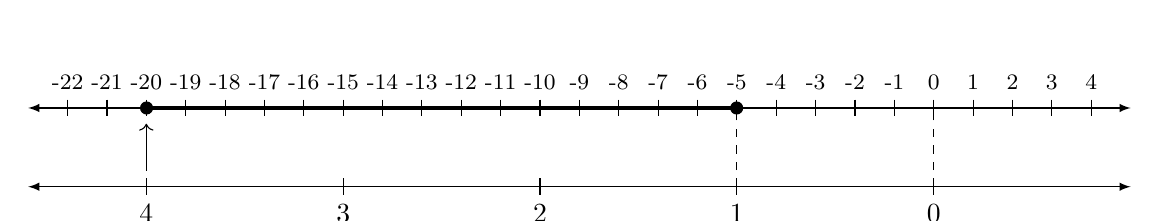
\begin{tikzpicture}
% Adapted from http://tex.stackexchange.com/questions/148252/
\draw[latex-latex] (-5.5,0) -- (8.5,0) ; 
\foreach \x in  {-22,-21,...,4}
\draw[shift={(0.5*\x+6,0)}] (0pt,3pt) -- (0pt,-3pt);
\foreach \x in {-22,-21,...,4}
\draw[shift={(0.5*\x+6,0)}] (0pt,0pt) -- (0pt,3pt) node[above] {$\text{\footnotesize\x}$};
\draw[*-*] (-4.08,0) -- (3.58,0);
\draw[very thick] (-4,0) -- (3.5,0);

\draw[latex-latex] (-5.5,-1) -- (8.5,-1) ; 
\foreach \x in  {0,1,2,3,4}
\draw[shift={(6-2.5*\x,-1)},color=black] (0pt,3pt) -- (0pt,-3pt);
\foreach \x in {0,1,2,3,4}
\draw[shift={(6-2.5*\x,-1)},color=black] (0pt,0pt) -- (0pt,-3pt) node[below] {$\x$};
\draw[dashed] (6,-1) -- (6,0) ;
\draw[dashed] (3.5,-1) -- (3.5,0) ;
\draw[->] (-4,-0.8) -- (-4,-0.2) ;
\end{tikzpicture}}
\end{center}
\end{itemize}

\begin{exercise}
Interpret the operations of subtraction and division as geometric transformations of the real number line.
\end{exercise}

We will take for granted the arithmetic properties of the real numbers in this chapter, waiting until \Cref{secInequalitiesMeans} to sink our teeth into the details. For example, we will take for granted the basic properties of rational numbers, for instance
\[ \frac{a}{b}+\frac{c}{d} = \frac{ad+bc}{bd} \quad \text{and} \quad \frac{a}{b} \cdot \frac{c}{d} = \frac{ac}{bd} \]

\subsection*{Rational and irrational numbers}
\label{pGettingStartedRationalNumbers}

Before we can talk about irrational numbers, we should say what they are.

\begin{definition}
\label{defIrrationalNumber}
\index{irrational number}
An \textbf{irrational number} is a real number that is not rational.
\end{definition}

Unlike $\mathbb{N},\mathbb{Z},\mathbb{Q},\mathbb{R},\mathbb{C}$, there is no standard single letter expressing the irrational numbers. However, by the end of \Cref{secSetOperations}, we will be able to write the set of irrational numbers as $\mathbb{R} \setminus \mathbb{Q}$.

Note in particular that `irrational' does not simply mean `not rational'---that would imply that all complex numbers which are not real are irrational---rather, the term `irrational' means `real and not rational'.

Proving that a real number is \textit{irrational} is not particularly easy. We will get our foot in the door by allowing ourselves to assume the following result, which is restated and proved in \Cref{propSqrt2Irrational}.

\begin{proposition}
\label{propSqrt2IrrationalPreliminary}
The real number $\sqrt{2}$ is irrational. \qed
\end{proposition}

We can use the fact that $\sqrt{2}$ is irrational to prove some facts about the relationship between rational numbers and irrational numbers.

\begin{proposition}
Let $a$ and $b$ be irrational numbers. It is possible that $ab$ be rational.
\end{proposition}

\begin{cproof}
Let $a=b=\sqrt{2}$. Then $a$ and $b$ are irrational, and $ab=2=\frac{2}{1}$, which is rational.
\end{cproof}

\begin{exercise}
Let $r$ be a rational number and let $a$ be an irrational number. Prove that it is possible that $ra$ be rational, and it is possible that $ra$ be irrational.
\end{exercise}

\subsection*{Complex numbers ($\mathbb{C}$)}

We have seen that multiplication by real numbers corresponds with scaling and reflection of the number line---scaling alone when the multiplicand is positive, and scaling with reflection when it is negative. We could alternatively interpret this reflection as a \textit{rotation} by half a turn, since the effect on the number line is the same. You might then wonder what happens if we rotate by arbitrary angles, rather than only half turns.

What we end up with is a \textit{plane} of numbers, not merely a line---see \Cref{figComplexNumbers}. Moreover, it happens that the rules that we expect arithmetic operations to satisfy still hold---addition corresponds with translation, and multiplication corresponds with scaling and rotation. This resulting number set is that of the \textit{complex numbers}.

\begin{definition}
\label{defComplexNumbersInformal}
The \textbf{complex numbers} are those obtained by the non-negative real numbers upon rotation by any angle about the point $0$. We write $\mathbb{C}$ \inlatex{mathbb\{C\}}\lindexmmc{mathbb}{$\mathbb{A}, \mathbb{B}, \dots$} for the set of all complex numbers; thus, the notation `$z \in \mathbb{C}$' means that $z$ is a complex number.
\end{definition}

\begin{figure}[p!]
\centering
\resizebox{\textwidth}{!}{
\begin{tikzpicture}
\draw[latex-latex] (-5.5,0) -- (5.5,0) ;
\draw[latex-latex, dotted] (-4.76, 2.75) -- (4.76, -2.75) ;
\draw[latex-latex, dotted] (-2.75, 4.76) -- (2.75, -4.76) ;
\draw[latex-latex, dotted] (0, -5.5) -- (0, 5.5) ;
\draw[latex-latex, dotted] (2.75, 4.76) -- (-2.75, -4.76) ;
\draw[latex-latex, dotted] (4.76, 2.75) -- (-4.76, -2.75) ;
\draw[dotted] (0,0) circle [radius=1] ;
\draw[dotted] (0,0) circle [radius=2] ;
\draw[dotted] (0,0) circle [radius=3] ;
\draw[dotted] (0,0) circle [radius=4] ;
\draw[dotted] (0,0) circle [radius=5] ;
\foreach \x in  {-5,-4,-3,-2,-1,0,1,2,3,4,5}
  \draw[shift={(\x,0)}] (0pt,3pt) -- (0pt,-3pt);
\foreach \x in {-5,-4,-3,-2,-1,0,1,2,3,4,5}
  \draw[shift={(\x,0)}] (0,0) node[below right] {$\text{\small\x}$};
\draw (0,1) node[above right] {$i$};
\draw (-3pt,1) -- (3pt,1);
\foreach \x in {2,3,4,5}
  \draw[shift={(0,\x)}] (0,0) node[above right] {$\x i$};
\foreach \x in {2,3,4,5}
  \draw[shift={(0,\x)}] (-3pt,0pt) -- (3pt, 0pt);
\foreach \x in {2,3,4,5}
  \draw[shift={(0,-\x)}] (0,0) node[below right] {$\text{\small-}\x i$};
\foreach \x in {2,3,4,5}
  \draw[shift={(0,-\x)}] (-3pt,0pt) -- (3pt, 0pt);
\draw (0,-1) node[below right] {$\text{\small-}i$};
\draw (-3pt,-1) -- (3pt,-1);
\end{tikzpicture}
}
\caption{Illustration of the complex plane, with some points labelled.}
\label{figComplexNumbers}
\end{figure}

There is a particularly important complex number, $i$, which is the point in the complex plane exactly one unit above $0$---this is illustrated in \Cref{figComplexNumbers}. Multiplication by $i$ has the effect of rotating the plane by a quarter turn anticlockwise. In particular, we have $i^2 = i \cdot i = -1$; the complex numbers have the astonishing property that square roots of \textit{all} complex numbers exist (including all the real numbers).

In fact, every complex number can be written in the form $a+bi$, where $a,b \in \mathbb{R}$; this number corresponds with the point on the complex plane obtained by moving $a$ units to the right and $b$ units up, reversing directions as usual if $a$ or $b$ is negative. Arithmetic on the complex numbers works just as with the real numbers; in particular, using the fact that $i^2=-1$, we obtain
\[ (a+bi)+(c+di) = (a+c)+(b+d)i \quad \text{and} \quad (a+bi) \cdot (c+di) = (ac-bd) + (ad+bc)i \]

We will discuss complex numbers further in the portion of this chapter on polynomials below.

\subsection*{Polynomials}
\label{pGettingStartedPolynomials}

The integers, rational numbers, real numbers and complex numbers are all examples of \textit{rings}, which means that they come equipped with nicely behaving notions of addition, subtraction and multiplication.

\begin{definition}
\label{defPolynomialPreliminary}
\index{polynomial}
Let $A$ be one $\mathbb{Z}$, $\mathbb{Q}$, $\mathbb{R}$ or $\mathbb{C}$. A (\textbf{univariate}) \textbf{polynomial over $A$} in the \textbf{indeterminate} $x$ is an expression of the form
\[ a_0 + a_1x + \cdots + a_nx^n \]
where $n \in \mathbb{N}$ and each $a_k \in A$. The numbers $a_k$ are called the \textbf{coefficients} of the polynomial. If not all coefficients are zero, the largest value of $k$ for which $a_k \ne 0$ is called the \textbf{degree} of the polynomial. By convention, the degree of the polynomial $0$ is $-\infty$.
\end{definition}

Polynomials of degree $1$, $2$, $3$, $4$ and $5$ are respectively called \textit{linear}, \textit{quadratic}, \textit{cubic}, \textit{quartic} and \textit{quintic} polynomials.

\begin{example}
The following expressions are all polynomials:
\[ 3 \qquad 2x-1 \qquad (3+i)x^2-x \]
Their degrees are $0$, $1$ and $2$, respectively. The first two are polynomials over $\mathbb{Z}$, and the third is a polynomial over $\mathbb{C}$.
\end{example}

\begin{exercise}
Write down a polynomial of degree $4$ over $\mathbb{R}$ which is not a polynomial over $\mathbb{Q}$.
\end{exercise}

\begin{notation}
Instead of writing out the coefficients of a polynomial each time, we may write something like $p(x)$ or $q(x)$. The `$(x)$' indicates that $x$ is the indeterminate of the polynomial. If $\alpha$ is a number\footnote{When dealing with polynomials, we will typically reserve the letter $x$ for the indeterminate variable, and use the Greek letters $\alpha,\beta,\gamma$ \inlatex{alpha, \textbackslash{}beta, \textbackslash{}gamma} for numbers to be substituted into a polynomial.} and $p(x)$ is a polynomial in indeterminate $x$, we write $p(\alpha)$ for the result of \textbf{substituting} $\alpha$ for $x$ in the expression $p(x)$.
\end{notation}

Note that, if $A$ is any of the sets $\mathbb{N}$, $\mathbb{Z}$, $\mathbb{Q}$, $\mathbb{R}$ or $\mathbb{C}$, and $p(x)$ is a polynomial over $A$, then $p(\alpha) \in A$ for all $\alpha \in A$.

\begin{example}
Let $p(x)=x^3-3x^2+3x-1$. Then $p(x)$ is a polynomial over $\mathbb{Z}$ with indeterminate $x$. For any integer $\alpha$, the value $p(\alpha)$ will also be an integer. For example
\[ p(0) = 0^3-3 \cdot 0^2 + 3 \cdot 0 - 1 = -1 \quad \text{and} \quad p(3) = 3^3 - 3 \cdot 3^2 + 3 \cdot 3 - 1 = 8 \]
\end{example}

\begin{definition}
\label{defRootOfPolynomial}
\index{root}
Let $p(x)$ be a polynomial. A \textbf{root} of $p(x)$ is a complex number $\alpha$ such that $p(\alpha)=0$.
\end{definition}

The \textit{quadratic formula} (\Cref{thmQuadraticFormula}) tells us that the roots of the polynomial $x^2+ax+b$, where $a,b \in \mathbb{C}$, are precisely the complex numbers
\[ \frac{-a+\sqrt{a^2-4b}}{2} \quad \text{and} \quad \frac{-a-\sqrt{a^2-4b}}{2} \]

Note our avoidance of the symbol `$\pm$', which is commonly found in discussions of quadratic polynomials. The symbol `$\pm$' is dangerous because it may suppress the word `and' or the word `or', depending on context---this kind of ambiguity is not something that we will want to deal with when discussing the logical structure of a proposition in \Cref{chLogicalStructure}!

\begin{example}
\label{exApplicationOfQuadraticFormula}
Let $p(x)=x^2-2x+5$. The quadratic formula tells us that the roots of $p$ are
\begin{center}
$\dfrac{2 + \sqrt{4 - 4 \cdot 5}}{2} = 1 + \sqrt{-4} = 1+2i$
\quad and \quad
$\dfrac{2 - \sqrt{4 - 4 \cdot 5}}{2} = 1-\sqrt{-4} = 1-2i$
\end{center}
The numbers $1+2i$ and $1-2i$ are related in that their real parts are equal and their imaginary parts differ only by a sign. \Cref{exComplexNumberAsRootOfQuadraticOverR} generalises this observation.
\end{example}

\begin{exercise}
\label{exComplexNumberAsRootOfQuadraticOverR}
Let $\alpha = a+bi$ be a complex number, where $a,b \in \mathbb{R}$. Prove that $\alpha$ is the root of a quadratic polynomial over $\mathbb{R}$, and find the other root of this polynomial.
\end{exercise}

The following exercise proves the well-known result which classifies the number of real roots of a polynomial over $\mathbb{R}$ in terms of its coefficients.

\begin{exercise}
\label{exDiscriminantRealRoots}
\index{discriminant}
Let $a,b \in \mathbb{C}$ and let $p(x)=x^2+ax+b$. The value $\Delta=a^2-4b$ is called the \textbf{discriminant} of $p$. Prove that $p$ has two roots if $\Delta \ne 0$ and one root if $\Delta = 0$. Moreover, if $a,b \in \mathbb{R}$, prove that $p$ has no real roots if $\Delta < 0$, one real root if $\Delta = 0$, and two real roots if $\Delta > 0$.
\end{exercise}

\begin{example}
Consider the polynomial $x^2-2x+5$. Its discriminant is equal to $(-2)^2-4 \cdot 5 = -16$, which is negative. \Cref{exDiscriminantRealRoots} tells us that it has two roots, neither of which are real. This was verified by \Cref{exApplicationOfQuadraticFormula}, where we found that the roots of $x^2-2x+5$ are $1+2i$ and $1-2i$.

Now consider the polynomial $x^2-2x-3$. Its discriminant is equal to $(-2)^2-4\cdot(-3) = 16$, which is positive. \Cref{exDiscriminantRealRoots} tells us that it has two roots, both of which are real; and indeed
\[ x^2-2x-3 = (x+1)(x-3) \]
so the roots of $x^2-2x-3$ are $-1$ and $3$.
\end{example}

% Chapter exercises
\chexbegin{chGettingStarted}
\numberitemswithin{section}
\begin{chapex}
For each of the following binary operations on $\mathbb{Z}$, determine whether it is: (i) associative, (ii) unital, (iii) commutative.
\begin{multicols}{2}
\begin{enumerate}[(a)]
\item $a \star b = ab$
\item $a \star b = ab + a + b$
\item $a \star b = a^b$
\item $a \star b = |b - a|$
\item $a \star b = a$
\item $a \star b = a + b + 1$
\end{enumerate}
\end{multicols}
\end{chapex}
\chexend

\part{Core concepts}
\label{ptCoreConcepts}

\chapter{Logical structure}
    \label{chLogicalStructure}
    \renewcommand{\currentchapter}{01}

% !TeX root = ../../book.tex



\newpage
% !TeX root = ../../book.tex
\section{Propositional logic}
\secbegin{secPropositionalLogic}

Every mathematical proof is written in the context of certain \textit{assumptions} being made, and certain \textit{goals} to be achieved.

\begin{itemize}
\item \textbf{Assumptions} are the propositions which are known to be true, or which we are assuming to be true for the purposes of proving something. They include theorems that have already been proved, prior knowledge which is assumed of the reader, and assumptions which are explicitly made using words like `suppose' or `assume'.
\item \textbf{Goals} are the propositions we are trying to prove in order to complete the proof of a result, or perhaps just a step in the proof.
\end{itemize}

With every phrase we write, our assumptions and goals change. This is perhaps best illustrated by example. In \Cref{exAssumptionsGoals} below, we will examine the proof of \Cref{propDivisibilityIsTransitive} in detail, so that we can see how the words we wrote affected the assumptions and goals at each stage in the proof. We will indicate our assumptions and goals at any given stage using tables---the assumptions listed will only be those assumptions which are made explicitly; prior knowledge and previously proved theorems will be left implicit.

\begin{example}
\label{exAssumptionsGoals}
The statement of \Cref{propDivisibilityIsTransitive} was as follows:
\begin{quote}
Let $a,b,c \in \mathbb{Z}$. If $c$ divides $b$ and $b$ divides $a$, then $c$ divides $a$.
\end{quote}
The set-up of the proposition instantly gives us our initial assumptions and goals:
\begin{center}
\begin{tabular}{C{150pt}|C{150pt}}
\textbf{Assumptions} & \textbf{Goals} \\ \hline
$a,b,c \in \mathbb{Z}$ & If $c$ divides $b$ and $b$ divides $a$, then $c$ divides $a$
\end{tabular}
\end{center}
We will now proceed through the proof, line by line, to see what effect the words we wrote had on the assumptions and goals.

Since our goal was an expression of the form `if\dots{}then\dots{}', it made sense to start by assuming the `if' statement, and using that assumption to prove the `then' statement. As such, the first thing we wrote in our proof was:
\begin{quote}
Suppose that $c$ divides $b$ and $b$ divides $a$.
\end{quote}
Our updated assumptions and goals are reflected in the following table.
\begin{center}
\begin{tabular}{C{150pt}|C{150pt}}
\textbf{Assumptions} & \textbf{Goals} \\ \hline
$a,b,c \in \mathbb{Z}$ & $c$ divides $a$ \\
$c$ divides $b$ & \\
$b$ divides $a$ & 
\end{tabular}
\end{center}

Our next step in the proof was to unpack the definitions of `$c$ divides $b$' and `$b$ divides $a$', giving us more to work with.

\begin{quote}
{\color{gray} Suppose that $c$ divides $b$ and $b$ divides $a$.} By \Cref{defDivisionPreliminary}, it follows that
\[
b=qc \quad \text{and} \quad a=rb
\]
for some integers $q$ and $r$.
\end{quote}

This introduces two new variables $q,r$ and allows us to replace the assumptions `$c$ divides $b$' and `$b$ divides $a$' with their definitions.

\begin{center}
\begin{tabular}{C{150pt}|C{150pt}}
\textbf{Assumptions} & \textbf{Goals} \\ \hline
$a,b,c,q,r \in \mathbb{Z}$ & $c$ divides $a$ \\
$b=qc$ & \\
$a=rb$ &
\end{tabular}
\end{center}

At this point we have pretty much exhausted all of the assumptions we can make, and so our attention turns towards the goal---that is, we must prove that $c$ divides $a$. At this point, it helps to `work backwards' by unpacking the goal: what does it mean for $c$ to divide $a$? Well, by \Cref{defDivisionPreliminary}, we need to prove that $a$ is equal to some integer multiplied by $c$---this will be reflected in the following table of assumptions and goals.

Since we are now trying to express $a$ in terms of $c$, it makes sense to use the equations we have relating $a$ with $b$, and $b$ with $c$, to relate $a$ with $c$.

\begin{quote}
{\color{gray} Suppose that $c$ divides $b$ and $b$ divides $a$. By \Cref{defDivisionPreliminary}, it follows that
\[
b=qc \quad \text{and} \quad a=rb
\]
for some integers $q$ and $r$.} Using the first equation, we may substitute $qc$ for $b$ in the second equation, to obtain
\[
a=r(qc)
\]
\end{quote}

We are now very close, as indicated in the following table.

\begin{center}
\begin{tabular}{C{150pt}|C{150pt}}
\textbf{Assumptions} & \textbf{Goals} \\ \hline
$a,b,c,q,r \in \mathbb{Z}$ & $a = [\text{some integer}] \cdot c$ \\
$b=qc$ & \\
$a=rb$ & \\
$a=r(qc)$ & 
\end{tabular}
\end{center}

Our final step was to observe that the goal has at last been achieved:

\begin{quote}
{\color{gray} Suppose that $c$ divides $b$ and $b$ divides $a$. By \Cref{defDivisionPreliminary}, it follows that
\[
b=qc \quad \text{and} \quad a=rb
\]
for some integers $q$ and $r$. Using the first equation, we may substitute $qc$ for $b$ in the second equation, to obtain}
\[
{\color{gray} a=r(qc)}
\]
But $r(qc) = (rq)c$, and $rq$ is an integer,
\end{quote}

\begin{center}
\begin{tabular}{C{150pt}|C{150pt}}
\textbf{Assumptions} & \textbf{Goals} \\ \hline
$a,b,c,q,r \in \mathbb{Z}$ &  \\
$b=qc$ & \\
$a=rb$ & \\
$a=r(qc)$ & \\
$a=(rq)c$ & \\
$rq \in \mathbb{Z}$ & 
\end{tabular}
\end{center}

Now that there is nothing left to prove, it is helpful to reiterate that point so that the reader has some closure on the matter.

\begin{quote}
{\color{gray} Suppose that $c$ divides $b$ and $b$ divides $a$. By \Cref{defDivisionPreliminary}, it follows that
\[
b=qc \quad \text{and} \quad a=rb
\]
for some integers $q$ and $r$. Using the first equation, we may substitute $qc$ for $b$ in the second equation, to obtain
\[
a=r(qc)
\]
But $r(qc) = (rq)c$, and $rq$ is an integer,} so it follows from \Cref{defDivisionPreliminary} that $c$ divides $a$.
\end{quote}
\end{example}

\subsection*{Symbolic logic}

Consider again the proposition that we proved in \Cref{propDivisibilityIsTransitive} (for given integers $a,b,c$):

\begin{center}
If $c$ divides $b$ and $b$ divides $a$, then $c$ divides $a$.
\end{center}

The three statements `$c$ divides $b$', `$b$ divides $a$' and `$c$ divides $a$' are all propositions in their own right, despite the fact that they all appear inside a more complex proposition. We can examine the logical structure of the proposition by replacing these simpler propositions with symbols, called \textit{propositional variables}. Writing $P$ to represent `$c$ divides $b$', $Q$ to represent `$b$ divides $a$' and $R$ to represent `$c$ divides $a$', we obtain:

\begin{center}
If $P$ and $Q$, then $R$.
\end{center}

Breaking down the proposition in this way makes it clear that a feasible \textit{assume} $P$ and $Q$, and then \textit{derive} $R$ from these assumptions---this is exactly what we did in the proof, which we examined in great detail in \Cref{exAssumptionsGoals}. But importantly, it suggests that the same proof strategy might work for other propositions which are also of the form `if $P$ and $Q$, then $R$', such as the following proposition (for a given integer $n$):

\begin{center}
If $n > 2$ and $n$ is prime, then $n$ is odd.
\end{center}

Observe that the simpler propositions are joined together to form a more complex proposition using language, namely the word `and' and the construction `if\dots{} then\dots{}'---we will represent these constructions symbolically using \textit{logical operators}, which will be introduced in \Cref{defLogicalOperator}.

Zooming in even more closely, we can use \Cref{defDivisionPreliminary} to observe that `$c$ divides $b$' really means `$b = qc$ for some $q \in \mathbb{Z}$'. The expression `for some $q \in \mathbb{Z}$' introduces a new variable $q$, which we must deal with appropriately in our proof. Words which we attach to variables in our proofs---such as `any', `exists', `all', `some', `unique' and `only'---will be represented symbolically using \textit{quantifiers}, which we will study in \Cref{secVariablesQuantifiers}.

By breaking down a complex proposition into simpler statements which are connected together using logical operators and quantifiers, we can more precisely identify what assumptions we can make at any given stage in a proof of the proposition, and what steps are needed in order to finish the proof.

\subsection*{Propositional formulae}

We begin our development of symbolic logic with some definitions to fix our terminology.

\begin{definition}
\label{defPropositionalVariable}
\index{propositional variable}
\index{truth value}
A \textbf{propositional variable} is a symbol that represents a proposition. Propositional variables may be assigned \textbf{truth values} (`true' or `false').
\end{definition}

We will typically use the lower-case letters $p$, $q$, $r$ and $s$ as our propositional variables.

We will be able to form more complex expressions representing propositions by connecting together simpler ones using \textit{logical operators} such as $\wedge$ (which represents `and'), $\vee$ (which represents `or'), $\Rightarrow$ (which represents `if\dots{}then\dots{}') and $\neg$ (which represents `not').

The definition of the notions of \textit{logical operator} and \textit{propositional formula} given below is a little bit difficult to digest, so it is best understood by considering examples of propositional formulae and instances of logical operators. Fortunately we will see plenty of these, since they are the central objects of study for the rest of this section.

\begin{definition}
\label{defPropositionalFormula}
\label{defLogicalOperator}
\index{logical operator}
\index{propositional formula}
\index{subformula}
A \textbf{propositional formula} is an expression that is either a propositional variable, or is built up from simpler propositional formulae (`subformulae') using a \textbf{\mbox{logical} \mbox{operator}}. In the latter case, the truth value of the propositional formula is determined by the truth values of the subformulae according to the rules of the logical operator.
\end{definition}

On first sight, \Cref{defPropositionalFormula} seems circular---it defines the term `propositional formula' in terms of propositional formulae! But in fact it is not circular; it is an example of a \textit{recursive} definition (we avoid circularity with the word `simpler'). To illustrate, consider the following example of a propositional formula:
\[
(p \wedge q) \Rightarrow r
\]
This expression represents a proposition of the form `if $p$ and $q$, then $r$', where $p,q,r$ are themselves propositions. It is built from the subformulae $p \wedge q$ and $r$ using the logical operator $\Rightarrow$, and $p \wedge q$ is itself built up from the subformulae $p$ and $q$ using the logical operator $\wedge$.

The truth value of $(p \wedge q) \Rightarrow r$ is then determined by the truth values of the constituent propositional variables ($p$, $q$ and $r$) according to the rules for the logical operators $\wedge$ and $\Rightarrow$.

If this all seems a bit abstract, that is because it \textit{is} abstract, and you are forgiven if it makes no sense to you yet. From this point onwards, we will only study particular instances of logical operators, which will make it all much easier to understand.

\subsubsection*{Conjunction (`and', $\wedge$)}

Conjunction is the logical operator which makes precise what we mean when we say `and'.

\begin{idefinition}
\label{defConjunction}
\index{conjunction}
\nindex{conjunction}{$\wedge$}{conjunction}
The \textbf{conjunction} operator is the logical operator $\wedge$ \inlatex{wedge}\lindexmmc{wedge}{$\wedge$}, defined according to the following rules:
\begin{itemize}
\item \introrule{\wedge} If $p$ is true and $q$ is true, then $p \wedge q$ is true;
\item \elimrulesub{\wedge}{1} If $p \wedge q$ is true, then $p$ is true;
\item \elimrulesub{\wedge}{2} If $p \wedge q$ is true, then $q$ is true.
\end{itemize}
The expression $p \wedge q$ represents `$p$ and $q$'.
\end{idefinition}

It is not always obvious when conjunction is being used; sometimes it sneaks in without the word `and' ever being mentioned! Be on the look-out for occasions like this, such as in the following exercise.

\begin{example}
\label{exSevenDividesTwentyEightConjunction}
We can express the proposition `$7$ is a prime factor of $28$' in the form $p \wedge q$, by letting $p$ represent the proposition `$7$ is prime' and letting $q$ represent the proposition `$7$ divides $28$'.
\end{example}

\begin{exercise}
\label{exJohnMathematicianPittsburgh}
Express the proposition `John is a mathematician who lives in Pittsburgh' in the form $p \wedge q$, for propositions $p$ and $q$.
\end{exercise}

The rules in \Cref{defConjunction} are examples of \textit{rules of inference}---they tell us how to deduce (or `infer') the truth of one propositional formula from the truth of other propositional formulae. In particular, rules of inference never directly tell us when a proposition is \textit{false}---in order to prove something is false, we will prove its \textit{negation} is true (see \Cref{defNegation}).

Rules of inference tell us how to use the logical structure of propositions in proofs:

\begin{itemize}
\item The rule \introrule{\wedge} is an \textit{introduction rule}, meaning that it tells us how to \textit{prove a goal} of the form $p \wedge q$---indeed, if we want to prove that $p \wedge q$ is true, \introrule{\wedge} tells us that it suffices to prove that $p$ is true and prove that $q$ is true.

\item The rules \elimrulesub{\wedge}{1} and \elimrulesub{\wedge}{2} are \textit{elimination rules}, meaning that they tell us how to \textit{use an assumption} of the form $p \wedge q$---indeed, if we are assuming that $p \wedge q$ is true, we are then free to use the fact that $p$ is true and the fact that $q$ is true.
\end{itemize}

Each logical operator will come equipped with some introduction and/or elimination rules, which tell us how to prove goals or use assumptions which include the logical operator in question. It is in this way that the logical structure of a proposition informs \textit{proof strategies}, like the following:

\begin{strategy}[Proving conjunctions]
\label{strProvingConjunctionsDirect}
A proof of the proposition $p \wedge q$ can be obtained by tying together two proofs, one being a proof that $p$ is true and one being a proof that $q$ is true.
\end{strategy}

\begin{example}
\label{exSevenDividesTwentyEightConjunctionProof}
Suppose we are required to prove that $7$ is a prime factor of $28$. In \Cref{exSevenDividesTwentyEightConjunction} we expressed `$7$ is a prime factor of $28$' as the conjunction of the propositions `$7$ is prime' and `$7$ divides $28$', and so \Cref{strProvingConjunctionsDirect} breaks down the proof into two steps: first prove that $7$ is prime, and then prove that $7$ divides $28$.
\end{example}

Much like \Cref{strProvingConjunctionsDirect} was informed by the introduction rule for $\wedge$, the elimination rules inform how we may make use of an assumption involving a conjunction.

\begin{strategy}[Assuming conjunctions]
\label{strAssumingConjunctionsDirect}
If an assumption in a proof has the form $p \wedge q$, then we may assume $p$ and assume $q$ in the proof.
\end{strategy}

\begin{example}
\label{exSevenDividesTwentyEightConjunctionAssumption}
Suppose that, somewhere in the process of proving a proposition, we arrive at the fact that $7$ is a prime factor of $28$. \Cref{strAssumingConjunctionsDirect} then allows us to use the separate facts that $7$ is prime and that $7$ divides $28$.
\end{example}

\Cref{strProvingConjunctionsDirect,strAssumingConjunctionsDirect} seem almost \textit{obvious}. To an extent they are obvious, and that is why we are stating them first. But the real reason we are going through the process of precisely defining logical operators, their introduction and elimination rules, and the corresponding proof strategies, is that when you are in the middle of the proof of a complicated result, it is all too easy to lose track of what you have already proved and what remains to be proved. Keeping track of the assumptions and goals in a proof, and understanding what must be done in order to complete the proof, is a difficult task.

To avoid drawing this process out too long, we need a compact way of expressing rules of inference that allows us to simply read off corresponding proof strategies. We \textit{could} use tables of assumptions and goals like in \Cref{exAssumptionsGoals}, but this quickly becomes clunky---indeed, even the very simple conjunction introduction rule \introrule{\wedge} doesn't look very nice in this format:

\begin{center}
\begin{tabular}{C{60pt}|C{60pt}}
{\small \textbf{Assumptions}} & {\small \textbf{Goals}} \\ \hline
$\vdots$ & $p \wedge q$ \\
$\vdots$ & ~
\end{tabular}
$\quad \leadsto \quad$
\begin{tabular}{C{60pt}|C{60pt}}
{\small \textbf{Assumptions}} & \small{\textbf{Goals}} \\ \hline
$\vdots$ & $p$ \\
$\vdots$ & $q$
\end{tabular}
\end{center}

Instead, we will represent rules of inference in the style of \textit{natural deduction}. In this style, we write the \textit{premises} $p_1,p_2,\dots,p_k$ of a rule above a line, with a single \textit{conclusion} $q$ below the line, representing the assertion that the truth of a proposition $q$ follows from the truth of (all of) the premises $p_1,p_2,\dots,p_k$.

\begin{center}
\begin{prooftree}
  \AxiomC{$p_1$}
  \AxiomC{$p_2$}
  \AxiomC{$\cdots$}
  \AxiomC{$p_k$}
\QuaternaryInfC{$q$}
\end{prooftree}
\end{center}

For instance, the introduction and elimination rules for conjunction can be expressed concisely follows:

\begin{center}
\begin{minipage}{0.15\textwidth}
\centering
\begin{prooftree}
  \AxiomC{$p$}
  \AxiomC{$q$}
\TagC{\introrule{\wedge}}
\BinaryInfC{$p \wedge q$}
\end{prooftree}
\end{minipage}
%
\hspace{20pt}
%
\begin{minipage}{0.15\textwidth}
\centering
\begin{prooftree}
  \AxiomC{$p \wedge q$}
\TagC{\elimrulesub{\wedge}{1}}
\UnaryInfC{$p$}
\end{prooftree}
\end{minipage}
%
\hspace{20pt}
%
\begin{minipage}{0.15\textwidth}
\centering
\begin{prooftree}
  \AxiomC{$p \wedge q$}
\TagC{\elimrulesub{\wedge}{2}}
\UnaryInfC{$q$}
\end{prooftree}
\end{minipage}
\end{center}

In addition to its clean and compact nature, this way of writing rules of inference is useful because we can combine them into \textit{proof trees} in order to see how to prove more complicated propositions. For example, consider the following proof tree, which combines two instances of the conjunction introduction rule.

\begin{center}
\begin{prooftree}
    \AxiomC{$p$}
    \AxiomC{$q$}
  \BinaryInfC{$p \wedge q$}
  \AxiomC{$r$}
\BinaryInfC{$(p \wedge q) \wedge r$}
\end{prooftree}
\end{center}

From this proof tree, we obtain a strategy for proving a proposition of the form $(p \wedge q) \wedge r$. Namely, first prove $p$ and prove $q$, to conclude $p \wedge q$; and then prove $r$, to conclude $(p \wedge q) \wedge r$. This illustrates that the logical structure of a proposition informs how we may structure a proof of the proposition.

\begin{exercise}
Write a proof tree whose conclusion is the propositional formula $(p \wedge q) \wedge (r \wedge s)$, where $p,q,r,s$ are propositional variables. Express `$2$ is an even prime number and $3$ is an odd prime number' in the form $(p \wedge q) \wedge (r \wedge s)$, for appropriate propositions $p$, $q$, $r$ and $s$, and describe how your proof tree suggests what a proof might look like.
\end{exercise}

\subsubsection*{Disjunction (`or', $\vee$)}

\begin{idefinition}
\label{defDisjunction}
\index{disjunction}
\nindex{disjunction}{$\vee$}{disjunction}
The \textbf{disjunction} operator is the logical operator $\vee$ \inlatex{vee}\lindexmmc{vee}{$\vee$}, defined according to the following rules:
\begin{itemize}
\item \introrulesub{\vee}{1} If $p$ is true, then $p \vee q$ is true;
\item \introrulesub{\vee}{2} If $q$ is true, then $p \vee q$ is true;
\item \elimrule{\vee} If $p \vee q$ is true, and if $r$ can be derived from $p$ and from $q$, then $r$ is true.
\end{itemize}
The expression $p \vee q$ represents `$p$ or $q$'.
\end{idefinition}

The introduction and elimination rules for disjunction are represented diagramatically as follows.

\begin{center}
\begin{minipage}[b]{0.15\textwidth}
\centering
\begin{prooftree}
  \AxiomC{$p$}
\TagC{\introrulesub{\vee}{1}}
\UnaryInfC{$p \vee q$}
\end{prooftree}
\end{minipage}
%
\hspace{20pt}
%
\begin{minipage}[b]{0.15\textwidth}
\centering
\begin{prooftree}
  \AxiomC{$q$}
\TagC{\introrulesub{\vee}{2}}
\UnaryInfC{$p \vee q$}
\end{prooftree}
\end{minipage}
%
\hspace{20pt}
%
\begin{minipage}[b]{0.35\textwidth}
\begin{prooftree}
  \AxiomC{$p \vee q$}
    \AxiomC{$[p]$}
    \noLine
    \UnaryInfC{$\downleadsto$}
  \noLine
  \UnaryInfC{$r$}
    \AxiomC{$[q]$}
    \noLine
    \UnaryInfC{$\downleadsto$}
  \noLine
  \UnaryInfC{$r$}
\TagC{\elimrule{\vee}}
\TrinaryInfC{$r$}
\end{prooftree}
\end{minipage}
\end{center}

We will discuss what the notation $[p] \leadsto r$ and $[q] \leadsto r$ means momentarily. First, we zoom in on how the disjunction introduction rules inform proofs of propositions of the form `$p$ or $q$'.

\begin{strategy}[Proving disjunctions]
\label{strProvingDisjunctionsDirect}
In order to prove a proposition of the form $p \vee q$, it suffices to prove just one of $p$ or $q$.
\end{strategy}

\begin{example}
Suppose we want prove that $8192$ is not divisible by $3$. We know by the division theorem (\Cref{thmDivisionPreliminary}) that an integer is not divisible by $3$ if and only if it leaves a remainder of $1$ or $2$ when divided by $3$, and so it suffices to prove the following:
\[
\begin{matrix} 8192 \text{ leaves a remainder of } 1 \\ \text{when divided by } 3 \end{matrix}
\quad \vee \quad
\begin{matrix} 8192 \text{ leaves a remainder of } 2 \\
\text{when divided by } 3 \end{matrix}
\]
A quick computation reveals that $8192 = 2730 \times 3 + 2$, so that $8192$ leaves a remainder of $2$ when divided by $3$. By \Cref{strProvingDisjunctionsDirect}, the proof is now complete, since the full disjunction follows by \introrulesub{\vee}{2}.
\end{example}

\begin{example}
Let $p,q,r,s$ be propositional variables. The propositional formula $(p \vee q) \wedge (r \vee s)$ represents `$p$ or $q$, and $r$ or $s$'. What follows are two examples of truth trees for this propositional formula.

\begin{center}
\begin{minipage}{0.3\textwidth}
\centering
\begin{prooftree}
    \AxiomC{$p$}
  \TagC{\introrulesub{\vee}{1}}
  \UnaryInfC{$p \vee q$}
    \AxiomC{$r$}
  \TagC{\introrulesub{\vee}{1}}
  \UnaryInfC{$r \vee s$}
\TagC{\introrule{\wedge}}
\BinaryInfC{$(p \vee q) \wedge (r \vee s)$}
\end{prooftree}
\end{minipage}
%
\hspace{20pt}
%
\begin{minipage}{0.3\textwidth}
\centering
\begin{prooftree}
    \AxiomC{$q$}
  \TagC{\introrulesub{\vee}{2}}
  \UnaryInfC{$p \vee q$}
    \AxiomC{$s$}
  \TagC{\introrulesub{\vee}{2}}
  \UnaryInfC{$r \vee s$}
\TagC{\introrule{\wedge}}
\BinaryInfC{$(p \vee q) \wedge (r \vee s)$}
\end{prooftree}
\end{minipage}
\end{center}

The proof tree on the left suggests the following proof strategy for $(p \vee q) \wedge (r \vee s)$. First prove $p$, and deduce $p \vee q$; then prove $r$, and deduce $r \vee s$; and finally deduce $(p \vee q) \wedge (r \vee s)$. The proof tree on the right suggests a different strategy, where $p \vee q$ is deduced by proving $q$ instead of $p$, and $r \vee s$ is deduced by proving $s$ instead of $r$.

Selecting which (if any) of these to use in a proof might depend on what we are trying to prove. For example, for a fixed natural number $n$, let $p$ represent `$n$ is even', let $q$ represent `$n$ is odd', let $r$ represent `$n \ge 2$' and let $s$ represent `$n$ is a perfect square'. Proving $(p \vee q) \wedge (r \vee s)$ when $n=2$ would be most easily done using the left-hand proof tree above, since $p$ and $r$ are evidently true when $n=2$. However, the second proof tree would be more appropriate for proving $(p \vee q) \wedge (r \vee s)$ when $n=1$.
\end{example}

\begin{aside}
If you haven't already mixed up $\wedge$ and $\vee$, you probably will soon, so here's a way of remembering which is which:
\begin{center} \vspace{-10pt} \large \textbf{fish n chips} \end{center}
\vspace{-10pt} If you forget whether it's $\wedge$ or $\vee$ that means `and', just write it in place of the `n' in `fish n chips':
\begin{center} \vspace{-10pt} fish $\wedge$ chips \qquad \qquad fish $\vee$ chips \end{center}
\vspace{-10pt} Clearly the first looks more correct, so $\wedge$ means `and'. If you don't eat fish (or chips), then worry not, as this mnemonic can be modified to accommodate a wide variety of dietary restrictions; for instance `mac n cheese' or `quinoa n kale' or, for the meat lovers, `ribs n brisket'.
\end{aside}

Recall the diagrammatic statement of the disjunction elimination rule:

\begin{center}
\begin{prooftree}
  \AxiomC{$p \vee q$}
    \AxiomC{$[p]$}
    \noLine
    \UnaryInfC{$\downleadsto$}
  \noLine
  \UnaryInfC{$r$}
    \AxiomC{$[q]$}
    \noLine
    \UnaryInfC{$\downleadsto$}
  \noLine
  \UnaryInfC{$r$}
\TagC{\elimrule{\vee}}
\TrinaryInfC{$r$}
\end{prooftree}
\end{center}

The curious notation $[p] \leadsto r$ indicates that $p$ is a \textit{temporary assumption}. In the part of the proof corresponding to $[p] \leadsto r$, we would assume that $p$ is true and derive $r$ from that assumption, and remove the assumption that $p$ is true from that point onwards. Likewise for $[q] \leadsto r$.

The proof strategy obtained from the disjunction elimination rule is called \textit{proof by cases}.

\begin{strategy}[Assuming disjunctions---proof by cases]
\label{strAssumingDisjunctionsDirect}
\index{proof!by cases}
If an assumption in a proof has the form $p \vee q$, then we may derive a proposition $r$ by splitting into two cases: first, derive $r$ from the temporary assumption that $p$ is true, and then derive $r$ from the assumption that $q$ is true.
\end{strategy}

The following example illustrates how \Cref{strProvingDisjunctionsDirect,strAssumingDisjunctionsDirect} can be used together in a proof.

\begin{example}
\label{exPositiveProperFactorOfFourEvenOrPerfectSquare}
Let $n$ be a positive proper factor of $4$, and suppose we want to prove that $n$ is either even or a perfect square.
\begin{itemize}
\item Our assumption that $n$ is a positive proper factor of $4$ can be expressed as the disjunction $n = 1 \vee n = 2$.
\item Our goal is to prove the disjunction `$n \text{ is even} \vee n \text{ is a perfect square}$'.
\end{itemize}

According to \Cref{strAssumingDisjunctionsDirect}, we split into two cases, one in which $n=1$ and one in which $n=2$. In each case, we must derive `$n \text{ is even} \vee n \text{ is a perfect square}$', for which it suffices by \Cref{strProvingDisjunctionsDirect} to derive either that $n$ is even or that $n$ is a perfect square. Thus a proof might look something like this:

\begin{quote}
Since $n$ is a positive proper factor of $4$, either $n=1$ or $n=2$.
\begin{itemize}
\item \textbf{Case 1.} Suppose $n=1$. Then since $1^2=1$ we have $n = 1^2$, so that $n$ is a perfect square.
\item \textbf{Case 2.} Suppose $n=2$. Then since $2 = 2 \times 1$, we have that $n$ is even.
\end{itemize}
Hence $n$ is either even or a perfect square. \qed
\end{quote}

Notice that in both Case 1 and Case 2, we did not explicitly mention that we had proved that `$n \text{ is even} \vee n \text{ is a perfect square}$', leaving that deduction to the reader---we only mentioned it after the proofs in each case were complete.
\end{example}

The proof of \Cref{propRemainderOfSquaresModulo3} below splits into \textit{three} cases, rather than just two.

\begin{proposition}
\label{propRemainderOfSquaresModulo3}
Let $n \in \mathbb{Z}$. Then $n^2$ leaves a remainder of $0$ or $1$ when divided by $3$.
\end{proposition}

\begin{cproof}
Let $n \in \mathbb{Z}$. By the division theorem (\Cref{thmDivisionPreliminary}), one of the following must be true for some $k \in \mathbb{Z}$:
\[
n=3k \quad \text{or} \quad n=3k+1 \quad \text{or} \quad n=3k+2
\]
\begin{itemize}
\item Suppose $n=3k$. Then
\[
n^2 = (3k)^2 = 9k^2 = 3 \cdot (3k^2)
\]
So $n^2$ leaves a remainder of $0$ when divided by $3$.
\item Suppose $n=3k+1$. Then
\[
n^2 = (3k+1)^2 = 9k^2+6k+1 = 3(3k^2+2k)+1
\]
So $n^2$ leaves a remainder of $1$ when divided by $3$.
\item Suppose $n=3k+2$. Then
\[
n^2 = (3k+2)^2 = 9k^2+12k+4 = 3(3k^2+4k+1)+1
\]
So $n^2$ leaves a remainder of $1$ when divided by $3$.
\end{itemize}
In all cases, $n^2$ leaves a remainder of $0$ or $1$ when divided by $3$.
\end{cproof}

Note that in the proof of \Cref{propRemainderOfSquaresModulo3}, unlike in \Cref{exPositiveProperFactorOfFourEvenOrPerfectSquare}, we did not explictly use the word `case', even though we were using proof by cases. Whether or not to make your proof strategies explicit is up to you---discussion of this kind of matter can be found in \Cref{secVocabulary}.

When completing the following exercises, try to keep track of exactly where you use the introduction and elimination rules that we have seen so far.

\begin{exercise}
Let $n$ be an integer. Prove that $n^2$ leaves a remainder of $0$, $1$ or $4$ when divided by $5$.
\hintlabel{exSquareRemainderModuloFive}{f
Mimic the proof of \Cref{propRemainderOfSquaresModulo3}.
}
\end{exercise}

\begin{exercise}
Let $a,b \in \mathbb{R}$ and suppose $a^2-4b \ne 0$. Let $\alpha$ and $\beta$ be the (distinct) roots of the polyonomial $x^2+ax+b$. Prove that there is a real number $c$ such that either $\alpha-\beta = c$ or $\alpha - \beta = ci$.
\end{exercise}

\subsubsection*{Implication (`if\dots{}then\dots{}', $\Rightarrow$)}

\begin{definition}
\label{defImplication}
\index{implication}
\nindex{implies}{$\Rightarrow$}{implication}
The \textbf{implication} operator is the logical operator $\Rightarrow$ \inlatex{Rightarrow}\lindexmmc{Rightarrow}{$\Rightarrow$}, defined according to the following rules:
\begin{itemize}
\item \introrule{\Rightarrow} If $q$ can be derived from the assumption that $p$ is true, then $p \Rightarrow q$ is true;
\item \elimrule{\Rightarrow} If $p \Rightarrow q$ is true and $p$ is true, then $q$ is true.
\end{itemize}
The expression $p \Rightarrow q$ represents `if $p$, then $q$'.
\end{definition}

\begin{center}
\begin{minipage}[b]{0.15\textwidth}
\begin{prooftree}
      \AxiomC{$[p]$}
    \noLine
    \UnaryInfC{$\downleadsto$}
  \noLine
  \UnaryInfC{$q$}
\TagC{\introrule{\Rightarrow}}
\UnaryInfC{$p \Rightarrow q$}
\end{prooftree}
\end{minipage}
%
\vspace{20pt}
%
\begin{minipage}[b]{0.3\textwidth}
\begin{prooftree}
  \AxiomC{$p \Rightarrow q$}
  \AxiomC{$p$}
\TagC{\elimrule{\Rightarrow}}
\BinaryInfC{$q$}
\end{prooftree}
\end{minipage}
\end{center}

\begin{strategy}[Proving implications]
\label{strProvingImplicationsDirect}
In order to prove a proposition of the form $p \Rightarrow q$, it suffices to assume that $p$ is true, and then derive $q$ from that assumption.
\end{strategy}

The following proposition illustrates how \Cref{strProvingImplicationsDirect} can be used in a proof.

\begin{proposition}
\label{propRationalTwoOfThree}
Let $x$ and $y$ be real numbers. If $x$ and $x+y$ are rational, then $y$ is rational.
\end{proposition}

\begin{cproof}
Suppose $x$ and $x+y$ are rational. Then there exist integers $a,b,c,d$ with $b,d \ne 0$ such that
\[
x = \frac{a}{b} \quad \text{and} \quad x+y = \frac{c}{d}
\]
It then follows that
\[
y = (x+y)-x = \frac{c}{d}-\frac{a}{b} = \frac{bc-ad}{bd}
\]
Since $bc-ad$ and $bd$ are integers, and $bd \ne 0$, it follows that $y$ is rational.
\end{cproof}

The key phrase in the above proof was `Suppose $x$ and $x+y$ are rational.' This introduced the assumptions $x \in \mathbb{Q}$ and $x+y \in \mathbb{Q}$, and reduced our goal to that of deriving a proof that $y$ is rational---this was the content of the rest of the proof.

\begin{exercise}
Let $p(x)$ be a polynomial over $\mathbb{C}$. Prove that if $\alpha$ is a root of $p(x)$, and $a \in \mathbb{C}$, then $\alpha$ is a root of $(x-a)p(x)$.
\end{exercise}

The elimination rule for implication \elimrule{\Rightarrow} is more commonly known by the Latin name \textit{modus ponens}.

\begin{strategy}[Assuming implications---modus ponens]
\label{strAssumingImplicationsDirect}
\index{modus ponens}
If an assumption in a proof has the form $p \Rightarrow q$, and $p$ is also assumed to be true, then we may deduce that $q$ is true.
\end{strategy}

\Cref{strAssumingDisjunctionsDirect} is frequently used to reduce a more complicated goal to a simpler one. Indeed, if we know that $p \Rightarrow q$ is true, and if $p$ is easy to verify, then it allows us to prove $q$ by proving $p$ instead.

\begin{example}
Let $f(x) = x^2+ax+b$ be a polynomial with $a,b \in \mathbb{R}$, and let $\Delta = a^2-4b$ be its discriminant. Part of \Cref{exDiscriminantRealRoots} was to prove that:
\begin{enumerate}[(i)]
\item If $\Delta > 0$, then $f$ has two real roots;
\item If $\Delta = 0$, then $f$ has one real root;
\item If $\Delta < 0$, then $f$ has no real roots.
\end{enumerate}
Given the polynomial $f(x) = x^2-68x+1156$, it would be a pain to go through the process of solving the equation $f(x)=0$ in order to determine how many real roots $f$ has. However, each of the propositions (i), (ii) and (iii) take the form $p \Rightarrow q$, so \Cref{strAssumingImplicationsDirect} reduces the problem of finding how many real roots $f$ has to that of evaluating $\Delta$ and comparing it with $0$. And indeed, $(-68)^2 - 4 \times 1156 = 0$, so the implication (ii) together with \elimrule{\Rightarrow} tell us that $f$ has one real root.
\end{example}

A common task faced by mathematicians is to prove that two conditions are equivalent. For example, given a polynomial $f(x) = x^2+ax+b$ with $a,b \in \mathbb{R}$, we know that \textit{if} $a^2-4b>0$ \textit{then} $f$ has two real roots, but is it also true that if $f$ has two real roots then $a^2-4b>0$? (The answer is `yes'.) The relationship between these two implications is that each is the \textit{converse} of the other.

\begin{definition}
\label{defConverse}
\index{converse}
The \textbf{converse} of a proposition of the form $p \Rightarrow q$ is the proposition $q \Rightarrow p$.
\end{definition}

A quick remark on terminology is pertinent. The following table summarises some common ways of referring to the propositions `$p \Rightarrow q$' and `$q \Rightarrow p$'.

\begin{center}
\begin{tabular}{c|c}
$p \Rightarrow q$ & $q \Rightarrow p$ \\ \hline
if $p$, then $q$ & if $q$, then $p$ \\
$p$ only if $q$ & $p$ if $q$ \\
$p$ is sufficient for $q$ & $p$ is necessary for $q$
\end{tabular}
\end{center}

We so often encounter the problem of proving both an implication and its converse that we introduce a new logical operator that represents the conjunction of both.

\begin{definition}
\label{defBiconditional}
\index{biconditional}
\nindex{biconditional}{$\Leftrightarrow$}{biconditional}
The \textbf{biconditional} operator is the logical operator $\Leftrightarrow$ \inlatex{Leftrightarrow}\lindexmmc{Leftrightarrow}{$\Leftrightarrow$}, defined by declaring $p \Leftrightarrow q$ to mean $(p \Rightarrow q) \wedge (q \Rightarrow p)$. The expression $p \Leftrightarrow q$ represents `$p$ if and only if $q$'.
\end{definition}

Many examples of biconditional statements come from solving equations; indeed, to say that the values $\alpha_1,\dots,\alpha_n$ are the solutions to a particular equation is precisely to say that
\[
x \text{ is a solution} \quad \Leftrightarrow \quad x = \alpha_1 \text{ or } x = \alpha_2 \text{ or } \cdots \text{ or } x = \alpha_n
\]

\begin{example}
\label{exSolveSqrtFirstExample}
We find all real solutions $x$ to the equation
\[
\sqrt{x-3} + \sqrt{x+4} = 7
\]
Let's rearrange the equation to find out what the possible solutions may be.
\begin{align*}
&\phantom{\Rightarrow\;\;} \sqrt{x-3} + \sqrt{x+4} = 7 && \\
&\Rightarrow (x-3) + 2\sqrt{(x-3)(x+4)} + (x+4) = 49 && \text{squaring} \\
&\Rightarrow 2\sqrt{(x-3)(x+4)} = 48-2x && \text{rearranging} \\
&\Rightarrow 4(x-3)(x+4) = (48-2x)^2 && \text{squaring} \\
&\Rightarrow 4x^2+4x-48 = 2304-192x+4x^2 && \text{expanding} \\
&\Rightarrow 196x = 2352 && \text{rearranging} \\
&\Rightarrow x=12 && \text{dividing by $196$}
\end{align*}
You might be inclined to stop here. Unfortunately, all we have proved is that, given a real number $x$, \textit{if} $x$ solves the equation $\sqrt{x-3} + \sqrt{x+4} = 7$, \textit{then} $x=12$. This narrows down the set of possible solutions to just one candidate---but we still need to check the converse, namely that \textit{if} $x=12$, \textit{then} $x$ is a solution to the equation.

As such, to finish off the proof, note that
\[
\sqrt{12-3} + \sqrt{12+4} = \sqrt{9} + \sqrt{16} = 3 + 4 = 7
\]
and so the value $x=12$ is indeed a solution to the equation.
\end{example}

The last step in \Cref{exSolveSqrtFirstExample} may have seemed a little bit silly; but \Cref{exSolveSqrtSecondExample} demonstrates that proving the converse when solving equations truly is necessary.

\begin{example}
\label{exSolveSqrtSecondExample}
We find all real solutions $x$ to the equation
\[
x+\sqrt{x}=0
\]
We proceed as before, rearranging the equation to find all possible solutions.
\begin{align*}
&\phantom{\Rightarrow\;\;} x+\sqrt{x} = 0 && \\
&\Rightarrow x=-\sqrt{x} && \text{rearranging} \\
&\Rightarrow x^2=x && \text{squaring} \\
&\Rightarrow x(x-1)=0 && \text{rearranging} \\
&\Rightarrow x=0 \text{ or } x=1 && 
\end{align*}
Now certainly $0$ is a solution to the equation, since
\[
0+\sqrt{0} = 0+0 = 0
\]
However, $1$ is \textit{not} a solution, since
\[
1+\sqrt{1} = 1+1 = 2
\]
Hence it is actually the case that, given a real number $x$, we have
\[
x+\sqrt{x} = 0 \quad \Leftrightarrow \quad x=0
\]
Checking the converse here was vital to our success in solving the equation!
\end{example}

A slightly more involved example of a biconditional statement arising from the solution to an equation---in fact, a class of equations---is the proof of the quadratic formula.

\begin{itheorem}[Quadratic formula]
\label{thmQuadraticFormula}
Let $a,b \in \mathbb{C}$. A complex number $\alpha$ is a root of the polynomial $x^2+ax+b$ if and only if
\[
\alpha = \frac{-a+\sqrt{a^2-4b}}{2} \quad \text{or} \quad \alpha =\frac{-a-\sqrt{a^2-4b}}{2}
\]
\end{itheorem}

\begin{cproof}
First we prove that \textit{if} $\alpha$ is a root, \textit{then} $\alpha$ is one of the values given in the statement of the proposition. So suppose $\alpha$ be a root of the polynomial $x^2+ax+b$. Then
\[
\alpha^2 + a\alpha + b = 0
\]
The algebraic technique of `completing the square' tells us that
\[
\alpha^2 + a\alpha = \left( \alpha + \frac{a}{2} \right)^2 - \frac{a^2}{4}
\]
and hence
\[
\left( \alpha + \frac{a}{2} \right)^2 - \frac{a^2}{4} + b = 0
\]
Rearranging yields
\[
\left( \alpha + \frac{a}{2} \right)^2  = \frac{a^2}{4} - b = \frac{a^2-4b}{4}
\]
Taking square roots gives
\[
\alpha + \frac{a}{2} = \frac{\sqrt{a^2-4b}}{2} \quad \text{or} \quad \alpha + \frac{a}{2} = \frac{-\sqrt{a^2-4b}}{2}
\]
and, finally, subtracting $\frac{a}{2}$ from both sides gives the desired result.

The proof of the converse is \Cref{exQuadraticFormulaConverse}.
\end{cproof}

\begin{exercise}
\label{exQuadraticFormulaConverse}
Complete the proof of the quadratic formula. That is, for fixed $a,b \in \mathbb{C}$, prove that if
\[
\alpha = \frac{-a+\sqrt{a^2-4b}}{2} \quad \text{or} \quad \alpha =\frac{-a-\sqrt{a^2-4b}}{2}
\]
then $\alpha$ is a root of the polynomial $x^2+ax+b$.
\end{exercise}

Another class of examples of biconditional propositions arise in finding necessary and sufficient criteria for an integer $n$ to be divisible by some number---for example, that an integer is divisible by $10$ if and only if its base-$10$ expansion ends with the digit $0$.

\begin{example}
\label{exTestForDivisibilityByEight}
Let $n \in \mathbb{N}$. We will prove that $n$ is divisible by $8$ if and only if the number formed of the last three digits of the base-$10$ expansion of $n$ is divisible by $8$.

First, we will do some `scratch work'. Let $d_rd_{r-1}\dots{}d_1d_0$ be the base-$10$ expansion of $n$. Then
\[
n = d_r \cdot 10^r + d_{r-1} \cdot 10^{r-1} + \cdots + d_1 \cdot 10 + d_0
\]
Define
\[
n' = d_2d_1d_0 \quad \text{and} \quad n'' = n-n' = d_rd_{r-1}\dots{}d_4d_3000
\]
Now $n-n' = 1000 \cdot d_rd_{r-1} \dots d_4d_3$ and $1000 = 8 \cdot 125$, so it follows that $8$ divides $n''$.

%% BEGIN EXTRACT (xtrStepsExample) %%
Our goal is now to prove that $8$ divides $n$ if and only if $8$ divides $n'$.

\begin{itemize}
\item ($\Rightarrow$) Suppose $8$ divides $n$. Since $8$ divides $n''$, it follows from \Cref{exDivisibilityIsLinear} that $8$ divides $an+bn''$ for all $a,b \in \mathbb{Z}$. But
\[
n' = n-(n-n') = n-n'' = 1 \cdot n + (-1) \cdot n''
\]
so indeed $8$ divides $n'$, as required.
\item ($\Leftarrow$)  Suppose $8$ divides $n'$. Since $8$ divides $n''$, it follows from \Cref{exDivisibilityIsLinear} that $8$ divides $an'+bn''$ for all $a,b \in \mathbb{Z}$. But
\[
n = n'+(n-n') = n'+n'' = 1 \cdot n' + 1 \cdot n''
\]
so indeed $8$ divides $n$, as required.
\end{itemize}
%% END EXTRACT
\end{example}

\begin{exercise}
Prove that a natural number $n$ is divisible by $3$ if and only if the sum of its base-$10$ digits is divisible by $3$.
\hintlabel{exSumOfDigitsDivisibleByThree}{%
Suppose $n = d_r \cdot 10^r + \cdots + d_1 \cdot 10 + d_0$ and let $s = d_r + \cdots + d_1 + d_0$. Start by proving that $3 \mid n-s$.
}
\end{exercise}

\subsubsection*{Negation (`not', $\neg$)}

So far we only officially know how to prove that true propositions are \textit{true}. The negation operator makes precise what we mean by `not', which allows us to prove that false propositions are \textit{false}.

\begin{definition}
\label{defContradiction}
\index{contradiction}
\nindex{contradiction}{$\bot$}{contradiction}
A \textbf{contradiction} is a proposition that is known or assumed to be false. We will use the symbol $\bot$ \inlatex{bot}\lindexmmc{bot}{$\bot$} to represent an arbitrary contradiction.
\end{definition}

\begin{example}
Some examples of contradictions include the assertion that $0=1$, or that $\sqrt{2}$ is rational, or that the equation $x^2=-1$ has a solution $x \in \mathbb{R}$.
\end{example}

\begin{definition}
\label{defNegation}
\index{negation}
\nindex{negation}{$\neg$}{negation}
The \textbf{negation} operator is the logical operator $\neg$ \inlatex{neg}\lindexmmc{neg}{$\neg$}, defined according to the following rules:
\begin{itemize}
\item \introrule{\neg} If a contradiction can be derived from the assumption that $p$ is true, then $\neg p$ is true;
\item \elimrule{\neg} If $\neg p$ and $p$ are both true, then a contradiction may be derived.
\end{itemize}
The expression $\neg p$ represents `not $p$' (or `$p$ is false').
\end{definition}

\begin{center}
\begin{minipage}[b]{0.2\textwidth}
\begin{prooftree}
      \AxiomC{$[p]$}
    \noLine
    \UnaryInfC{$\downleadsto$}
  \noLine
  \UnaryInfC{$\bot$}
\TagC{\introrule{\neg}}
\UnaryInfC{$\neg p$}
\end{prooftree}
\end{minipage}
%
\hspace{20pt}
%
\begin{minipage}[b]{0.2\textwidth}
\begin{prooftree}
  \AxiomC{$\neg p$}
  \AxiomC{$p$}
\TagC{\elimrule{\neg}}
\BinaryInfC{$\bot$}
\end{prooftree}
\end{minipage}
\end{center}

\begin{aside}
The rules \introrule{\neg} and \elimrule{\neg} closely resemble \introrule{\Rightarrow} and \elimrule{\Rightarrow}---indeed, we could simply define $\neg p$ to mean `$p \Rightarrow \bot$', where $\bot$ represents an arbitrary contradiction, but it will be easier later on to have a primitive notion of negation.
\end{aside}

The introduction rule for negation \introrule{\neg} gives rise to a proof strategy called \textit{proof by contradiction}, which turns out to be extremely useful.

\begin{strategy}[Proving negations---proof by contradiction]
\label{strProvingNegationsDirect}
\label{strProofByContradictionDirect}
\index{proof!by contradiction (direct)}
\index{contradiction!(direct) proof by}
In order to prove a proposition $p$ is false (that is, that $\neg p$ is true), it suffices to assume that $p$ is true and derive a contradiction.
\end{strategy}

The following proposition has a classic proof by contradiction.

\begin{proposition}
Let $r$ be a rational number and let $a$ be an irrational number. Then $r+a$ is irrational. 
\end{proposition}

\begin{cproof}
By \Cref{defIrrationalNumber}, we need to prove that $r+a$ is real and not rational. It is certainly real, since $r$ and $a$ are real, so it remains to prove that $r+a$ is not rational.

Suppose $r+a$ is rational. Since $r$ is rational, it follows from \Cref{propRationalTwoOfThree} that $a$ is rational, since
\[
a = (r+a) - r
\]
This contradicts the assumption that $a$ is irrational. It follows that $r+a$ is not rational, and is therefore irrational.
\end{cproof}

Now you can try proving some elementary facts by contradiction.

\begin{exercise}
\label{exNegationAndReciprocalOfIrrationalNumbers}
Let $x \in \mathbb{R}$. Prove by contradiction that if $x$ is irrational then $-x$ and $\frac{1}{x}$ are irrational.
\end{exercise}

\begin{exercise}
\label{exNoLeastPositiveReal}
Prove by contradiction that there is no least positive real number. That is, prove that there is not a positive real number $a$ such that $a \le b$ for all positive real numbers $b$.
\end{exercise}

A proof need not be a `proof by contradiction' in its entirety---indeed, it may be that only a small portion of the proof uses contradiction. This is exhibited in the proof of the following proposition.

\begin{proposition}
\label{propOddIffRemainderOfOne}
Let $a$ be an integer. Then $a$ is odd if and only if $a=2b+1$ for some integer $b$.
\end{proposition}
\begin{cproof}
Suppose $a$ is odd. By the division theorem (\Cref{thmDivisionPreliminary}), either $a=2b$ or $a=2b+1$, for some $b \in \mathbb{Z}$. If $a=2b$, then $2$ divides $a$, contradicting the assumption that $a$ is odd; so it must be the case that $a=2b+1$.

Conversely, suppose $a=2b+1$. Then $a$ leaves a remainder of $1$ when divided by $2$. However, by the division theorem, the even numbers are precisely those that leave a remainder of $0$ when divided by $2$. It follows that $a$ is not even, so is odd.
\end{cproof}

The elimination rule for the negation operator \elimrule{\neg} simply says that a proposition can't be true and false at the same time.

\begin{strategy}[Assuming negations]
\label{strAssumingNegations}
If an assumption in a proof has the form $\neg p$, then any derivation of $p$ leads to a contradiction.
\end{strategy}

The main use of \Cref{strAssumingNegations} is for obtaining the contradiction in a proof by contradiction---in fact, we have already used it in our examples of proof by contradiction! As such, we will not dwell on it further.

\subsection*{Logical axioms}

We wrap up this section by introducing a couple of additional logical rules (\textit{axioms}) that we will use in our proofs.

The first is the so-called \textit{law of excluded middle}, which appears so obvious that it is not even worth stating (let alone naming)---what it says is that every proposition is either true or false. But beware, as looks can be deceiving; the law of excluded middle is a non-constructive axiom, meaning that it should not be accepted in settings it is important to keep track of how a proposition is proved---simply knowing that a proposition is either true or false tells us nothing about how it might be proved or refuted. In most mathematical contexts, though, it is accepted without a second's thought.

\begin{axiom}[Law of excluded middle]
\label{axLEM}
\index{law of excluded middle}
Let $p$ be a propositional formula. Then $p \vee (\neg p)$ is true.
\end{axiom}

The law of excluded middle can be represented diagramatically as follows; there are no premises above the line, since we are simply asserting that it is true.

\begin{center}
\begin{prooftree}
  \AxiomC{}
\TagC{LEM}
\UnaryInfC{$p \vee (\neg p)$}
\end{prooftree}
\end{center}

\begin{strategy}[Using the law of excluded middle]
\label{strLEM}
In order to prove a proposition $q$ is true, it suffices to split into cases based on whether some other proposition $p$ is true or false, and prove that $q$ is true in each case.
\end{strategy}

The proof of \Cref{propIfProductEvenThenSomeFactorEven} below makes use of the law of excluded middle---note that we defined `odd' to mean `not even' (\Cref{defEvenOdd}).

\begin{proposition}
\label{propIfProductEvenThenSomeFactorEven}
Let $a,b \in \mathbb{Z}$. If $ab$ is even, then either $a$ is even or $b$ is even (or both).
\end{proposition}
\begin{cproof}
Suppose $a,b \in \mathbb{Z}$ with $ab$ even.
\begin{itemize}
\item Suppose $a$ is even---then we're done.
\item Suppose $a$ is odd. If $b$ is also odd, then by \Cref{propOddIffRemainderOfOne} can write
\[
a = 2k+1 \quad \text{and} \quad b=2\ell+1
\]
for some integers $k,\ell$. This implies that
\[
ab = (2k+1)(2\ell+1) = 4k\ell + 2k + 2\ell + 1 = 2(\underbrace{2k\ell + k + \ell}_{\in \mathbb{Z}}) + 1
\]
so that $ab$ is odd. This contradicts the assumption that $ab$ is even, and so $b$ must in fact be even.
\end{itemize}
In both cases, either $a$ or $b$ is even.
\end{cproof}

\begin{exercise}
Reflect on the proof of \Cref{propIfProductEvenThenSomeFactorEven}. Where in the proof did we use the law of excluded middle? Where in the proof did we use proof by contradiction? What was the contradiction in this case? Prove \Cref{propIfProductEvenThenSomeFactorEven} twice more, once using contradiction and not using the law of excluded middle, and once using the law of excluded middle and not using contradiction.
\end{exercise}

\begin{exercise}
Let $a$ and $b$ be irrational numbers. By considering the number $\sqrt{2}^{\sqrt{2}}$, prove that it is possible that $a^b$ be rational.
\hintlabel{exIrrationalExpIrrationalCanBeRational}{%
Use the law of excluded middle according to whether the proposition `$\sqrt{2}^{\sqrt{2}}$ is rational' is true or false.}
\end{exercise}

Another logical rule that we will use is the \textit{principle of explosion}, which is also known by its Latin name, \textit{ex falso sequitur quodlibet}, which approximately translates to `\textit{from falsity follows whatever you like}'.

\begin{axiom}[Principle of explosion]
\label{axPrincipleOfExplosion}
If a contradiction is assumed, any consequence may be derived.
\end{axiom}

\begin{center}
\begin{prooftree}
  \AxiomC{$\bot$}
\TagC{Expl}
\UnaryInfC{$p$}
\end{prooftree}
\end{center}

The principle of explosion is a bit confusing on first sight. To shed a tiny bit of intuition on it, think of it as saying that both true and false propositions are consequences of a contradictory assumption. For instance, suppose that $-1 = 1$. From this we can obtain consequences that are false, such as $0=2$ by adding $1$ to both sides of the equation, and consequences that are true, such as $1=1$ by squaring both sides of the equation.

We will rarely use the principle of explosion directly in our mathematical proofs, but we will use it in \Cref{secLogicalEquivalence} for proving logical formulae are equivalent.


\newpage
\section{Variables and quantifiers}
\secbegin{secVariablesQuantifiers}

\subsection*{Free and bound variables}

Everything we did in \Cref{secPropositionalLogic} concerned \textit{propositions} and the logical rules concerning their proofs. Unfortunately if all we have to work with is propositions then our ability to do mathematical reasoning will be halted pretty quickly. For example, consider the following statement:
\begin{center}
$x$ is divisible by $7$
\end{center}
This statement seems like the kind of thing we should probably be able to work with if we're doing mathematics. It makes sense if $x$ is a integer, such as $28$ or $41$; but it doesn't make sense at all if $x$ is a parrot called Alex.\footnote{Alex the parrot is the only non-human animal to have ever been observed to ask an existential question; he died in September 2007 so we may never know if he was divisible by $7$, but it is unlikely. According to \textit{Time}, his last words were `you be good, see you tomorrow, I love you'. The reader is advised to finish crying before they continue reading about variables and quantifiers.} In any case, even when it does make sense, its truth value depends on $x$; indeed, `$28$ is divisible by $7$' is a true proposition, but `$41$ is divisible by $7$' is a false proposition.

This means that the statement `$x$ is divisible by $7$' isn't a proposition---\textit{quel horreur}! But it \textit{almost} is a proposition: if we know that $x$ refers somehow to an integer, then it becomes a proposition as soon as a particular numerical value of $x$ is specified. The symbol $x$ is called a \textit{free variable}.

\begin{definition}
\label{defFreeVariable}
\index{free variable}
\index{bound variable}
\index{variable!free}
\index{variable!bound}
Let $x$ be a variable that is understood to refer to an element of a set $X$. In a statement involving $x$, we say $x$ is \textbf{free} if it makes sense to substitute particular elements of $X$ in the statement; otherwise, we say $x$ is \textbf{bound}.
\end{definition}

To represent statements that have free variables in them abstractly, we generalise the notion of a propositional variable (\Cref{defPropositionalVariable}) to that of a \textit{predicate}.

\begin{definition}
\label{defPredicate}
\index{predicate}
\index{domain of discourse}
\index{range!of a variable}
A \textbf{predicate} is a symbol $p$ together with a specified list of free variables $x_1, x_2, \dots, x_n$ (where $n \in \mathbb{N}$) and, for each free variable $x_i$, a specification of a set $X_i$ called the \textbf{domain of discourse} (or \textbf{range}) of $x_i$. We will typically write $p(x_1,x_2,\dots,x_n)$ in order to make the variables explicit.
\end{definition}

The statements represented by predicates are those that become propositions when specific values are substituted for their free variables from their respective domains of discourse. For example, `$x$ is divisible by $7$' is not a proposition, but it becomes a proposition when specific integers (such as $28$ or $41$) are substituted for $x$.

This is a lot to take in, so let's look at some examples.

\begin{example}
\label{exFirstExamplesOfPredicates}
\fixlistskip
\begin{enumerate}[(i)]
\item We can represent the statement `$x$ is divisible by $7$' discussed above by a predicate $p(x)$ whose only free variable $x$ has $\mathbb{Z}$ as its domain of discourse. Then $p(28)$ is the true proposition `$28$ is divisible by $7$' and $p(41)$ is the false proposition `$41$ is divisible by $7$'.
\item A predicate with no free variables is precisely a propositional variable. This means that the notion of a predicate generalises that of a propositional variable.
\item The expression `$2^n-1$ is prime' can be represented by a predicate $p(n)$ with one free variable $n$, whose domain of discourse is the set $\mathbb{N}$ of natural numbers. Then $p(3)$ is the true proposition `$2^3-1$ is prime' and $p(4)$ is the false proposition `$2^4-1$ is prime'.
\item The expression `$x-y$ is rational' can be represented by a predicate $q(x,y)$ with free variables $x$ and $y$, whose domain of discourse is the set $\mathbb{R}$ of real numbers.
\item The expression `there exist integers $a$ and $b$ such that $x = a^2+b^2$' has free variable $x$ and bound variables $a,b$. It can be represented by a predicate $r(x)$ with one free variable $x$, whose domain of discourse is $\mathbb{Z}$.
\item The expression `every even natural number $n \ge 2$ is divisible by $k$' has free variable $k$ and bound variable $n$. It can be represented by a predicate $s(k)$ with one free variable $k$, whose domain of discourse is $\mathbb{N}$.
\end{enumerate}
\end{example}



\subsection*{Quantifiers}

Look again at the statements in parts (v) and (vi) of \Cref{exFirstExamplesOfPredicates}. Both contained bound variables, which were so because we used words like `there exists' and `every'---had we not used these words, those variables would be free, as in `$x=a^2+b^2$' and `$n$ is divisible by $k$'.

Expressions that refer to \textit{how many} elements of a set make a statement true, such as `there exists' and `every', turn free variables into bound variables. We represent such expressions using symbols called \textit{quantifiers}, which are the central objects of study of this section.

The two main quantifiers used throughout mathematics are the \textit{universal} quantifier $\forall$ and the \textit{existential} quantifier $\exists$. We will define these quantifiers formally later in this section, but for now, the following informal definitions suffice:

\begin{itemize}
\item The expression `$\forall x \in X,\, \dots{}$' denotes `for all $x \in X$, \dots{}' and will be defined formally in \Cref{defUniversalQuantifier};
\item The expression `$\exists x \in X,\, \dots{}$' denotes `there exists $x \in X$ such that \dots{}' and will be defined formally in \Cref{defExistentialQuantifier}.
\end{itemize}

Note that we always place the quantifier \textit{before} the statement, so even though we might write or say things like `$n=2k$ for some integer $k$' or `$x^2 \ge 0$ for all $x \in \mathbb{R}$', we would express these statements symbolically as `$\exists k \in \mathbb{Z},\, n=2k$' and `$\forall x \in \mathbb{R},\, x^2 \ge 0$', respectively.

We will define a third quantifier $\exists !$ in terms of $\forall$ and $\exists$ to say that there is \textit{exactly one} element of a set making a statement true. There are plenty of other quantifiers out there, but they tend to be specific to particular fields---examples include `almost everywhere' in measure theory, `almost surely' in probability theory, `for all but finitely many' in set theory and related disciplines, and `for fresh' in the theory of nominal sets.

Using predicates, logical formulae and quantifiers, we are able to build up more complicated expressions, called \textit{logical formulae}. Logical formulae generalise propositional formulae (\Cref{defPropositionalFormula}) in by allowing (free and bound) variables and quantification to occur.

\begin{definition}
\label{defLogicalFormula}
\index{logical formula}
A \textbf{logical formula} is an expression that is built from predicates using logical operators and quantifiers; it may have both free and bound variables. The truth value of a logical formula depends on its free variables according to the rules for logical operators and quantifiers.
\end{definition}

Translating between plain English statements and purely symbolic logical formulae is an important skill to obtain:
\begin{itemize}
\item The plain English statements are easier to understand and are the kinds of things you would speak aloud or write down when discussing the mathematical ideas involved.
\item The symbolic logical formulae are what provide the precision needed to guide a proof of the statement being discussed---we will see strategies for proving statements involving quantifiers soon.
\end{itemize}

The following examples and exercise concern translating between plain English statements and purely symbolic logical formulae.

\begin{example}
Recall that an integer $n$ is even if and only if it is divisible by $2$. According to \Cref{defDivisionPreliminary}, that is to say that `$n$ is even' means `$n=2k$ for some integer $k$'. Using quantifiers, we can express `$n$ is even' as `$\exists k \in \mathbb{Z},\, n=2k$'.

The (false) proposition `every integer is even' can then be written symbolically as follows. First introduce a variable $n$ to refer to an integer; to say `every integer is even' is to say `$\forall n \in \mathbb{Z},\, n \text{ is even}$', and so using the symbolic representation of `$n$ is even', we can express `every integer is even' as $\forall n \in \mathbb{Z},\, \exists k \in \mathbb{Z},\, n=2k$'.
\end{example}

\begin{exercise}
\label{exEnglishToLogicalFormulae}
Find logical formulae that represent each of the following English statements.
\begin{enumerate}[(a)]
\item There is an integer that is divisible by every integer.
\item There is no greatest odd integer.
\item Between any two distinct rational numbers is a third distinct rational number.
\item If an integer has a rational square root, then that root is an integer.
\end{enumerate}
\end{exercise}

\begin{example}
Consider the following logical formula.

\[\forall a \in \mathbb{R},\, (a \ge 0 \Rightarrow \exists b \in \mathbb{R},\, a = b^2)\]

If we translate this expression symbol-for-symbol, what it says is:
\begin{center}
For every real number $a$, if $a$ is non-negative,\\
then there exists a real number $b$ such that $a=b^2$.
\end{center}

Read in this way, it is not a particularly enlightening statement. However, we can distill the robotic nature of the symbol-for-symbol reading by thinking more carefully about what the statement \textit{really} means.

Indeed, to say `$a = b^2$ for some real number $b$' is exactly to say that $a$ has a real square root---after all, what is a square root of $a$ if not a real number whose square is equal to $a$? This translation eliminates explicit reference to the bound variable $b$, so that the statement now reads:

\begin{center}
For every real number $a$, if $a$ is non-negative, then $a$ has a real square root.
\end{center}

We're getting closer. Next note that instead of the clunky expression `for every real number $a$, if $a$ is non-negative, then \dots{}', we could just say `for every non-negative real number $a$, \dots{}'.

\begin{center}
For every non-negative real number $a$, $a$ has a real square root.
\end{center}

Finally, we can eliminate the bound variable $a$ by simply saying:

\begin{center}
Every non-negative real number has a real square root.
\end{center}

This is now a meaningful expression that is much easier to understand than the logical formula we started with.
\end{example}

\begin{exercise}
\label{exLogicalFormulaeToEnglish}
Find statements in plain English, involving as few variables as possible, that are represented by each of the following logical formulae. (The domains of discourse of the free variables are indicated in each case.)
\begin{enumerate}[(a)]
\item $\exists q \in \mathbb{Z},\, a = qb$ --- free variables $a, b \in \mathbb{Z}$
\item $\exists a \in \mathbb{Z},\, \exists b \in \mathbb{Z},\, (b \ne 0 \wedge bx = a)$ --- free variable $x \in \mathbb{R}$
\item $\forall d \in \mathbb{N},\, [(\exists q \in \mathbb{Z},\, n=qd) \Rightarrow (d = 1 \vee d = n)]$ --- free variable $n \in \mathbb{N}$
\item $\forall a \in \mathbb{R},\, [a > 0 \Rightarrow \exists b \in \mathbb{R},\, (b > 0 \wedge a < b)]$ --- no free variables
\end{enumerate}
\end{exercise}

Now that we have a better understanding of how to translate between plain English statements and logical formulae, we are ready to give a precise mathematical treatment of quantifiers. Just like with logical operators in \Cref{secPropositionalLogic}, quantifiers will be defined according to \textit{introduction rules}, which tell us how to prove a quantified formula, and \textit{elimination rules}, which tell us how to use an assumption that involves a quantifier.

\subsubsection*{Universal quantification (`for all', $\forall$)}

The universal quantifier makes precise what we mean when we say `for all', or `$p(x)$ is always true no matter what value $x$ takes'.

\begin{definition}
\label{defUniversalQuantifier}
\index{universal quantifier}
\index{quantifier!universal}
The \textbf{universal quantifier} is the quantifier $\forall$ \inlatex{forall}\lindexmmc{forall}{$\forall$}; if $p(x)$ is a logical formula with free variable $x$ with range $X$, then $\forall x \in X,\, p(x)$ is the logical formula defined according to the following rules:
\begin{itemize}
\item \introrule{\forall} If $p(x)$ can be derived from the assumption that $x$ is an arbitrary element of $X$, then $\forall x \in X,\, p(x)$;
\item \elimrule{\forall} If $a \in X$ and $\forall x \in X,\, p(x)$ is true, then $p(a)$ is true.
\end{itemize}
The expression $\forall x \in X,\, p(x)$ represents `for all $x \in X$, $p(x)$'.
\end{definition}

\begin{center}
\begin{minipage}[b]{0.2\textwidth}
\centering
\begin{prooftree}
      \AxiomC{$[x \in X]$}
    \noLine
    \UnaryInfC{$\downleadsto$}
  \noLine
  \UnaryInfC{$p(x)$}
\UnaryInfC{$\forall x \in X,\, p(x)$}
\end{prooftree}
\end{minipage}
%
\hspace{20pt}
%
\begin{minipage}[b]{0.2\textwidth}
\centering
\begin{prooftree}
  \AxiomC{$\forall x \in X,\, p(x)$}
  \AxiomC{$a \in X$}
\BinaryInfC{$p(a)$}
\end{prooftree}
\end{minipage}
\end{center}

\begin{strategy}[Proving universally quantified statements]
\label{strProvingUniversal}
To prove a proposition of the form $\forall x \in X,\, p(x)$, it suffices to prove $p(x)$ for an arbitrary element $x \in X$---in other words, prove $p(x)$ whilst assuming nothing about the variable $x$ other than that it is an element of $X$.
\end{strategy}

Useful phrases for introducing an arbitrary variable of a set $X$ in a proof include `fix $x \in X$' or `let $x \in X$' or `take $x \in X$'---more on this is discussed in \Cref{secVocabulary}.

The proofs of the following propositions illustrate how a proof of a universally quantified statement might look.

\begin{proposition}
\label{exSquareOfOddIntegerIsOdd}
The square of every odd integer is odd.
\end{proposition}

\begin{cproof}
Let $n$ be an odd integer. Then $n=2k+1$ for some $k \in \mathbb{Z}$ by the division theorem (\Cref{thmDivisionPreliminary}), and so
\[n^2 = (2k+1)^2 = 4k^2+4k+1 = 2(2k^2+2k) + 1\]
Since $2k^2+2k \in \mathbb{Z}$, we have that $n^2$ is odd, as required.
\end{cproof}

Note that in the proof of \Cref{exSquareOfOddIntegerIsOdd}, we did not assume anything about $n$ other than that it is an odd integer.

\begin{proposition}
The base-$10$ expansion of the square of every natural number ends in one of the digits $0$, $1$, $4$, $5$, $6$ or $9$.
\end{proposition}

\begin{cproof}
Fix $n \in \mathbb{N}$, and let
\[n=d_rd_{r-1} \dots d_0\]
be its base-$10$ expansion. Write
\[n=10m+d_0\]
where $m \in \mathbb{N}$---that is, $m$ is the natural number obtained by removing the final digit from $n$. Then
\[n^2=100m^2+20md_0+d_0^2 = 10m(10m+2d_0)+d_0^2\]
Hence the final digit of $n^2$ is equal to the final digit of $d_0^2$. But the possible values of $d_0^2$ are
\[0 \quad 1 \quad 4 \quad 9 \quad 16 \quad 25 \quad 36 \quad 49 \quad 64 \quad 81\]
all of which end in one of the digits $0$, $1$, $4$, $5$, $6$ or $9$.
\end{cproof}

\begin{exercise}
\label{exEveryIntegerIsRational}
Prove that every integer is rational.
\end{exercise}

\begin{exercise}
Prove that every linear polynomial over $\mathbb{Q}$ has a rational root.
\end{exercise}

\begin{exercise}
Prove that, for all real numbers $x$ and $y$, if $x$ is irrational, then $x+y$ and $x-y$ are not both rational.
\hintlabel{exIrrationalPlusMinusRealNotBothRational}{%
Consider the sum of $x+y$ and $x-y$.
}
\end{exercise}

Before advancing too much further, beware of the following common error that arises when dealing with universal quantifiers.

\begin{commonerror}
Consider the following (non-)proof of the proposition $\forall n \in \mathbb{Z},\, n^2 \ge 0$.

\begin{quote}
Let $n$ be an arbitrary integer, say $n=17$. Then $17^2 = 289 \ge 0$, so the statement is true.
\end{quote}

The error made here is that the \textit{writer} has picked an arbitrary value of $n$, not the \textit{reader}. (In fact, the above argument actually proves $\exists n \in \mathbb{Z},\, n^2 \ge 0$.)

The proof should make no assumptions about the value of $n$ other than that it is an integer. Here is a correct proof:

\begin{quote}
Let $n$ be an arbitrary integer. Either $n \ge 0$ or $n < 0$. If $n \ge 0$ then $n^2 \ge 0$, since the product of two nonnegative numbers is nonnegative; if $n<0$ then $n^2 \ge 0$, since the product of two negative numbers is positive.
\end{quote}
\end{commonerror}

The strategy suggested by the elimination rule for the universal quantifier is one that we use almost without thinking about it.

\begin{strategy}[Assuming universally quantified statements]
\label{strAssumingUniversal}
If an assumption in a proof has the form $\forall x \in X,\, p(x)$, then we may assume that $p(a)$ is true whenever $a$ is an element of $X$.
\end{strategy}

\subsubsection*{Existential quantification (`there exists', $\exists$)}

\begin{definition}
\label{defExistentialQuantifier}
\index{existential quantifier}
\index{quantifier!existential}
The \textbf{existential quantifier} is the quantifier $\exists$ \inlatex{exists}\nindex{exists}{$\exists$}; if $p(x)$ is a logical formula with free variable $x$ with range $X$, then $\exists x \in X,\, p(x)$ is the logical formula defined according to the following rules:
\begin{itemize}
\item \introrule{\exists} If $a \in X$ and $p(a)$ is true, then $\exists x \in X,\, p(x)$;
\item \elimrule{\exists} If $\exists x \in X,\, p(x)$ is true, and $q$ can be derived from the assumption that $p(a)$ is true for some fixed $a \in X$, then $q$ is true.
\end{itemize}
The expression $\exists x \in X,\, p(x)$ represents `there exists $x \in X$ such that $p(x)$'.
\end{definition}

\begin{center}
\begin{minipage}[b]{0.25\textwidth}
\centering
\begin{prooftree}
  \AxiomC{$a \in X$}
  \AxiomC{$p(a)$}
\TagC{\introrule{\exists}}
\BinaryInfC{$\exists x \in X,\, p(x)$}
\end{prooftree}
\end{minipage}
%
\hspace{20pt}
%
\begin{minipage}[b]{0.4\textwidth}
\centering
\begin{prooftree}
  \AxiomC{$\exists x \in X,\, p(x)$}
      \AxiomC{$[a \in X], [p(a)]$}
    \noLine
  \UnaryInfC{$\downleadsto$}
  \noLine
\UnaryInfC{$q$}
\TagC{\elimrule{\exists}}
\BinaryInfC{$q$}
\end{prooftree}
\end{minipage}
\end{center}

\begin{strategy}[Proving existentially quantified statements]
\label{strProvingExistential}
To prove a proposition of the form $\exists x \in X,\, p(x)$, it suffices to prove $p(a)$ for some specific element $a \in X$, which should be explicitly defined.
\end{strategy}

\begin{example}
We prove that there is a natural number that is a perfect square and is one more than a perfect cube. That is, we prove
\[\exists n \in \mathbb{N},\, ([\exists k \in \mathbb{Z},\, n=k^2] \wedge [\exists \ell \in \mathbb{Z},\, n=\ell^3 + 1])\]
So define $n=9$. Then $n=3^2$ and $n=2^3+1$, so that $n$ is a perfect square and is one more than a perfect cube, as required.
\end{example}

The following proposition involves an existentially quantified statement---indeed, to say that a polynomial $f(x)$ has a real root is to say $\exists x \in \mathbb{R},\, f(x) = 0$.

\begin{proposition}
Fix $a \in \mathbb{R}$. The cubic polynomial $x^3 + (1-a^2)x - a$ has a real root.
\end{proposition}
\begin{cproof}
Let $f(x)=x^3+(1-a^2)x-a$. Define $x=a$; then
\[f(x) = f(a) = a^3 + (1-a^2)a - a = a^3 + a - a^3 - a = 0\]
Hence $a$ is a root of $f(x)$. Since $a$ is real, $f(x)$ has a real root.
\end{cproof}

The following exercises require you to prove existentially quantified statements.

\begin{exercise}
Prove that there is a real number which is irrational but whose square is rational.
\end{exercise}

\begin{exercise}
Prove that there is an integer which is divisible by zero.
\hintlabel{exZeroDividesSomeInteger}{%
Look carefully at the definition of divisibility (\Cref{defDivisionPreliminary}).
}
\end{exercise}

\begin{example}
Prove that, for all $x,y \in \mathbb{Q}$, if $x < y$ then there is some $z \in \mathbb{Q}$ with $x<z<y$.
\end{example}

The elimination rule for the existential quantifier gives rise to the following proof strategy.

\begin{strategy}[Assuming existentially quantified statements]
\label{strAssumingExistential}
If an assumption in the proof has the form $\exists x \in X,\, p(x)$, then we may introduce a new variable $a \in X$ and assume that $p(a)$ is true.
\end{strategy}

It ought to be said that when using existential elimination in a proof, the variable $a$ used to denote a particular element of $X$ for which $p(a)$ is true should not already be in use earlier in the proof.

\Cref{strAssumingExistential} is very useful in proofs of divisibility, since the expression `$a$ divides $b$' is an existentially quantified statement---this was \Cref{exLogicalFormulaeToEnglish}(a).

\begin{proposition}
Let $n \in \mathbb{Z}$. If $n^3$ is divisible by $3$, then $(n+1)^3 - 1$ is divisible by $3$.
\end{proposition}

\begin{cproof}
Suppose $n^3$ is divisible by $3$. Take $q \in \mathbb{Z}$ such that $n^3 = 3q$. Then
\begin{align*}
& (n+1)^3 - 1 && \\
&= (n^3 + 3n^2 + 3n + 1) - 1 && \text{expanding} \\
&= n^3 + 3n^2 + 3n && \text{simplifying} \\
&= 3q + 3n^2 + 3n && \text{since $n^3 = 3q$} \\
&= 3(q+n^2+n) && \text{factorising}
\end{align*}
Since $q+n^2+n \in \mathbb{Z}$, we have proved that $(n+1)^3 - 1$ is divisible by $3$, as required.
\end{cproof}

\subsubsection*{Uniqueness}

The concept of uniqueness arises whenever we want to use the word `the'. For example, in \Cref{defBaseBExpansionPreliminary} we defined the base-$b$ expansion of a natural number $n$ to be \textit{the} string $d_r d_{r-1} \dots d_1 d_0$ satisfying some properties. The issue with the word `the' here is that we don't know ahead of time whether a natural number $n$ may have base-$b$ expansions other than $d_r d_{r-1} \dots d_1 d_0$---this fact actually requires proof. To prove this fact, we would need to assume that $e_s e_{s-1} \dots e_1 e_0$ were another base-$b$ expansion of $n$, and prove that the strings $d_r d_{r-1} \dots d_1 d_0$ and $e_s e_{s-1} \dots e_1 e_0$ are the same---this is done in \Cref{thmBaseBExpansion}.

Uniqueness is typically coupled with \textit{existence}, since we usually want to know if there is \textit{exactly one} object satisfying a property. This motivates the definition of the \textit{unique existential} quantifier, which encodes what we mean when we say `there is exactly one $x \in X$ such that $p(x)$ is true'. The `existence' part ensures that at least one $x \in X$ makes $p(x)$ true; the `uniqueness' part ensures that $x$ is the only element of $X$ making $p(x)$ true.

\begin{definition}
\label{defUniqueExistentialQuantifier}
\index{quantifier!unique existential}
The \textbf{unique existential quantifier} is the quantifier $\exists !$ (\inlatex{exists!}\lindexmmc{\exists!}{$\exists!$}) defined such that $\exists ! x \in X,\, p(x)$ is shorthand for
\[(\underbrace{\exists x \in X,\, p(x)}_{\text{existence}}) ~ \wedge ~ (\underbrace{\forall a \in X,\, \forall b \in X,\, [p(a) \wedge p(b) \Rightarrow a=b]}_{\text{uniqueness}})\]
\end{definition}

\begin{example}
\label{exEveryPositiveRealHasUniqueSquareRoot}
Every positive real number has a unique positive square root. We can write this symbolically as
\[\forall a \in \mathbb{R},\, (a > 0 \Rightarrow \exists ! b \in \mathbb{R},\, (b > 0 \wedge b^2=a))\]
Reading this from left to right, this says: for every real number $a$, if $a$ is positive, then there exists a unique real number $b$, which is positive and whose square is $a$. 
\end{example}

\begin{discussion}
Explain why \Cref{defUniqueExistentialQuantifier} captures the notion of there being `exactly one' element $x \in X$ making $p(x)$ true. Can you think of any other ways that $\exists ! x \in X,\, p(x)$ could be defined?
\end{discussion}

\begin{strategy}[Proving unique-existentially quantified statements]
A proof of a statement of the form $\exists ! x \in X,\, p(x)$, consists of two parts:
\begin{itemize}
\item \textbf{Existence} --- prove that $\exists x \in X,\, p(x)$ is true (e.g.\ using \Cref{strProvingExistential});
\item \textbf{Uniqueness} --- let $a,b \in X$, assume that $p(a)$ and $p(b)$ are true, and derive $a=b$.
\end{itemize}

Alternatively, prove existence to obtain a fixed $a \in X$ such that $p(a)$ is true, and then prove $\forall x \in X,\, [p(x) \Rightarrow x=a]$.
\end{strategy}

\begin{example}
\label{exEveryPositiveRealHasUniqueSquareRootProof}
We prove \Cref{exEveryPositiveRealHasUniqueSquareRoot}, namely that for each real $a>0$ there is a unique $b>0$ such that $b^2=a$. So first fix $a > 0$.
\begin{itemize}
\item (\textbf{Existence}) The real number $\sqrt{a}$ is positive and satisfies $(\sqrt{a})^2=a$ by definition. Its existence will be deferred to a later time, but an informal argument for its existence could be provided using `number line' arguments as in \Cref{chGettingStarted}.
\item (\textbf{Uniqueness}) Let $y,z > 0$ be real numbers such that $y^2=a$ and $z^2=a$. Then $y^2=z^2$. Rearranging and factorising yields
\[(y-z)(y+z)=0\]
so either $y-z=0$ or $y+z=0$. If $y+z=0$ then $z=-y$, and since $y>0$, this means that $z<0$. But this contradicts the assumption that $z>0$. As such, it must be the case that $y-z=0$, and hence $y=z$, as required.
\end{itemize}
\end{example}

\begin{exercise}
\label{exExamplesOfUniqueExistentialQuantifier}
For each of the propositions, write it out as a logical formula involving the $\exists !$ quantifier and then prove it, using the structure of the logical formula as a guide.
\begin{enumerate}[(a)]
\item For each real number $a$, the equation $x^2+2ax+a^2=0$ has exactly one real solution $x$.
\item There is a unique real number $a$ for which the equation $x^2+a^2=0$ has a real solution $x$.
\item There is a unique natural number with exactly one positive divisor.
\end{enumerate}
\end{exercise}

The unique existential quantifier will play a large role when we study functions in \Cref{secFunctions}.

\subsection*{Quantifier alternation}
\index{quantifier alternation}
Compare the following two statements:
\begin{enumerate}[(i)] 
\item For every door, there is a key that can unlock it.
\item There is a key that can unlock every door.
\end{enumerate}

Letting the variables $x$ and $y$ refer to doors and keys, respectively, and letting $p(x,y)$ be the statement `door $x$ can be unlocked by key $y$', we can formulate these statements as:
\begin{enumerate}[(i)] 
\item $\forall x,\, \exists y,\, p(x,y)$
\item $\exists y,\, \forall x,\, p(x,y)$
\end{enumerate}

This is a typical `real-world' example of what is known as \textit{quantifier alternation}---the two statements differ only by the order of the front-loaded quantifiers, and yet they say very different things. Statement (i) requires every door to be unlockable, but the keys might be different for different doors; statement (ii), however, implies the existence of some kind of `master key' that can unlock all the doors.

Here's another example with a more mathematical nature:

\begin{exercise}
Let $p(x,y)$ be the statement `$x + y$ is even'.
\begin{itemize}
\item Prove that $\forall x \in \mathbb{Z},\, \exists y \in \mathbb{Z},\, p(x,y)$ is true.
\item Prove that $\exists y \in \mathbb{Z},\, \forall x \in \mathbb{Z},\, p(x,y)$ is false.
\end{itemize}
\end{exercise}

In both of the foregoing examples, you might have noticed that the `$\forall\exists$' statement says something \textit{weaker} than the `$\exists\forall$' statement---in some sense, it is easier to make a $\forall\exists$ statement true than it is to make an $\exists\forall$ statement true.

This idea is formalised in \Cref{thmQuantifierAlternation} below, which despite its abstract nature, has an extremely simple proof.

\begin{theorem} \label{thmQuantifierAlternation}
Let $p(x,y)$ be a logical formula with free variables $x \in X$ and $y \in Y$. Then
\[\exists y \in Y,\, \forall x \in X,\, p(x,y) \Rightarrow \forall x \in X,\, \exists y \in Y,\, p(x,y)\]
\end{theorem}

\begin{cproof}
Suppose $\exists y \in Y,\, \forall x \in X,\, p(x,y)$ is true. We need to prove $\forall x \in X,\, \exists y \in Y,\, p(x,y)$, so fix $a \in X$---our goal is now to prove $\exists y \in Y,\, p(a,y)$.

Using our assumption $\exists y \in Y,\, \forall x \in X,\, p(x,y)$, we may choose $b \in Y$ such that $\forall x,\, p(x,b)$ is true. But then $p(a, b)$ is true, so we have proved $\exists y \in Y,\, p(a,y)$, as required.
\end{cproof}

Statements of the form $\exists y \in Y,\, \forall x \in X,\, p(x,y)$ imply some kind of \textit{uniformity}: a value of $y$ making $\forall x \in X,\, p(x,y)$ true can be thought of as a `one size fits all' solution to the problem of proving $p(x,y)$ for a given $x \in X$. Later in your studies, it is likely that you will encounter the word `uniform' many times---it is precisely this notion of quantifier alternation that the word `uniform' refers to.

\newpage
% !TeX root = ../../book.tex
\section{Logical equivalence}
\secbegin{secLogicalEquivalence}

We motivate the content of this section with an example.

\begin{example}
\label{exNoEvenPrimeGreaterThanTwo}
Consider the following two logical formulae, where $P$ denotes the set of all prime numbers.
\begin{enumerate}[(1)]
\item $\forall n \in P,\, (n > 2 \Rightarrow [\exists k \in \mathbb{Z},\, n=2k+1])$;
\item $\neg \exists n \in P,\, (n > 2 \wedge [\exists k \in \mathbb{Z},\, n=2k])$.
\end{enumerate}
The logical formula (1) translates to `every prime number greater than two is odd', and the logical formula (2) translates to `there does not exist an even prime number greater than two'. These statements are evidently \textit{equivalent}---they mean the same thing---but they suggest different proof strategies:

\begin{enumerate}[(1)]
\item Fix a prime number $n$, assume that $n>2$, and then prove that $n = 2k+1$ for some $k \in \mathbb{Z}$.
\item Assume that there is some prime number $n$ such that $n>2$ and $n=2k$ for some $k \in \mathbb{Z}$, and derive a contradiction.
\end{enumerate}

While statement (1) more directly translates the plain English statement `every prime number greater than two is odd', it is the proof strategy suggested by (2) that is easier to use. Indeed, if $n$ is a prime number such that $n>2$ and $n=2k$ for some $k \in \mathbb{Z}$, then $2$ is a divisor of $n$ other than $1$ and $n$ (since $1<2<n$), contradicting the assumption that $n$ is prime.
\end{example}

The notion of \textit{logical equivalence}, captures precisely the sense in which the logical formulae in (1) and (2) in \Cref{exNoEvenPrimeGreaterThanTwo} `mean the same thing'. Being able to transform a logical formula into a different (but equivalent) form allows us to identify a wider range of feasible proof strategies.

\begin{definition}
\label{defLogicalEquivalence}
\index{logical equivalence}
\index{equivalence!logical}
\nindex{logical equivalence}{$\equiv$}{logical equivalence}
Let $p$ and $q$ be logical formulae. We say that $p$ and $q$ are \textbf{logically equivalent}, and write $p \equiv q$ \inlatex{equiv}\lindexmmc{equiv}{$\equiv$}, if $q$ can be derived from $p$ and $p$ can be derived from $q$.
\end{definition}

\subsection*{Logical equivalence of propositional formulae}

While \Cref{defLogicalEquivalence} defines logical equivalence between arbitrary logical formulae, we will start by focusing our attention on logical equivalence between \textit{propositional} formulae, like those we saw in \Cref{secPropositionalLogic}.

First, let's look at a couple of examples of what proofs of logical equivalence might look like. Be warned---they're not very nice to read! But there is light at the end of the tunnel. After struggling through \Cref{exConjunctionDistributesOverDisjunction,exImplicationInTermsOfDisjunction} and \Cref{exPAndQImpliesRIffPImpliesRAndQImpliesR}, we will introduce a very quick and easy tool for proving propositional formulae are logically equivalent.

\begin{example}
\label{exConjunctionDistributesOverDisjunction}
We demonstrate that $p \wedge (q \vee r) \equiv (p \wedge q) \vee (p \wedge r)$, where $p$, $q$ and $r$ are propositional variables.

\begin{itemize}
\item First assume that $p \wedge (q \vee r)$ is true. Then $p$ is true and $q \vee r$ is true by definition of conjunction. By definition of disjunction, either $q$ is true or $r$ is true.
\begin{itemize}
\item If $q$ is true, then $p \wedge q$ is true by definition of conjunction.
\item If $r$ is true, then $p \wedge r$ is true by definition of conjunction.
\end{itemize}
In both cases we have that $(p \wedge q) \vee (p \wedge r)$ is true by definition of disjunction.

\item Now assume that $(p \wedge q) \vee (p \wedge r)$ is true. Then either $p \wedge q$ is true or $p \wedge r$ is true, by definition of disjunction.
\begin{itemize}
\item If $p \wedge q$ is true, then $p$ is true and $q$ is true by definition of conjunction.
\item If $p \wedge r$ is true, then $p$ is true and $r$ is true by definition of conjunction.
\end{itemize}
In both cases we have that $p$ is true, and that $q \vee r$ is true by definition of disjunction. Hence $p \wedge (q \vee r)$ is true by definition of conjunction.
\end{itemize}

Since we can derive $(p \wedge q) \vee (p \wedge r)$ from $p \wedge (q \vee r)$ and vice versa, it follows that
\[ p \wedge (q \vee r) \equiv (p \wedge q) \vee (p \wedge r)\]
as required.
\end{example}

\begin{example}
\label{exImplicationInTermsOfDisjunction}
We prove that $p \Rightarrow q \equiv (\neg p) \vee q$, where $p$, $q$ and $r$ are propositional variables.

\begin{itemize}
\item First assume that $p \Rightarrow q$ is true. By the law of exluded middle (\Cref{axLEM}), either $p$ is true or $\neg p$ is true---we derive $(\neg p) \vee q$ in each case.
\begin{itemize}
\item If $p$ is true, then since $p \Rightarrow q$ is true, it follows from \elimrule{\Rightarrow} that $q$ is true, and so $(\neg p) \vee q$ is true by \introrulesub{\vee}{2};
\item If $\neg p$ is true, then $(\neg p) \vee q$ is true by \introrulesub{\vee}{1}.
\end{itemize}
In both cases, we see that $(\neg p) \vee q$ is true.

\item Now assume that $(\neg p) \vee q$ is true. To prove that $p \Rightarrow q$ is true, it suffices by \introrule{\Rightarrow} to assume that $p$ is true and derive $q$. So assume $p$ is true. Since $(\neg p) \vee q$ is true, we have that either $\neg p$ is true or $q$ is true.
\begin{itemize}
\item If $\neg p$ is true, then we obtain a contradiction from the assumption that $p$ is true, and so $q$ is true by the principle of explosion (\Cref{axPrincipleOfExplosion}).
\item If $q$ is true\dots{} well, then $q$ is true---there is nothing more to prove!
\end{itemize}
In both cases we have that $q$ is true. Hence $p \Rightarrow q$ is true.
\end{itemize}

We have derived $(\neg p) \vee q$ from $p \Rightarrow q$ and vice versa, and so the two formulae are logically equivalent.
\end{example}

\begin{exercise}
\label{exPAndQImpliesRIffPImpliesRAndQImpliesR}
Let $p$, $q$ and $r$ be propositional variables. Prove that the propositional formula $(p \vee q) \Rightarrow r$ is logically equivalent to $(p \Rightarrow r) \wedge (q \Rightarrow r)$.
\end{exercise}

Working through the derivations each time we want to prove logical equivalence can become cumbersome even for small examples like \Cref{exConjunctionDistributesOverDisjunction,exImplicationInTermsOfDisjunction} and \Cref{exPAndQImpliesRIffPImpliesRAndQImpliesR}.

The following theorem reduces the problem of proving logical equivalence between \textit{propositional} formulae to the purely algorithmic task of checking when the formulae are true and when they are false in a (relatively) small list of cases. We will streamline this process even further using \textit{truth tables} (\Cref{defTruthTable}).

\begin{theorem}
\label{thmLogicalEquivalentIffSameTruthValues}
Two propositional formulae are logically equivalent if and only if their truth values are the same under any assignment of truth values to their constituent propositional variables.
\end{theorem}

\begin{cidea}
A formal proof of this fact is slightly beyond our reach at this point, although we will be able to prove it formally by \textit{structural induction}, introduced in \Cref{secStructuralInduction}.

The idea of the proof is that, since propositional formulae are built up from simpler propositional formulae using logical operators, the truth value of a more complex propositional formula is determined by the truth values of its simpler subformulae. If we keep `chasing' these subformulae, we end up with just propositional variables.

For example, the truth value of $(p \Rightarrow r) \wedge (q \Rightarrow r)$ is determined by the truth values of $p \Rightarrow r$ and $q \Rightarrow r$ according to the rules for the conjunction operator $\wedge$. In turn, the truth value of $p \Rightarrow r$ is determined by the truth values of $p$ and $r$ according to the implication operator $\Rightarrow$, and the truth value of $q \Rightarrow r$ is determined by the truth values of $q$ and $r$ according to the implication operator again. It follows that the truth value of the whole propositional formula $(p \Rightarrow r) \wedge (q \Rightarrow r)$ is determined by the truth values of $p,q,r$ according to the rules for $\wedge$ and $\Rightarrow$.

If some assignment of truth values to propositional variables makes one propositional formula true but another false, then it must be impossible to derive one from the other---otherwise we'd obtain a contradiction. Hence both propositional formulae must have the same truth values no matter what assignment of truth values is given to their constituent propositional variables.
\end{cidea}

We now develop a systematic way of checking the truth values of a propositional formula under each assignment of truth values to its constituent propositional variables.

\begin{definition}
\label{defTruthTable}
\index{truth table}
The \textbf{truth table} of a propositional formula is the table with one row for each possible assignment of truth values to its constituent propositional variables, and one column for each subformula (including the propositional variables and the propositional formula itself). The entries of the truth table are the truth values of the subformulae.
\end{definition}

\begin{example}
\label{exNegationConjunctionDisjunctionImplicationTruthTable}
The following are the truth tables for $\neg p$, $p \wedge q$, $p \vee q$ and $p \Rightarrow q$.

\begin{center}
\begin{tabular}{c|c}
$p$ & $\neg p$ \\ \hline
\TT & \FF \\
\FF & \TT \\
\multicolumn{2}{c}{\phantom{\TT}\phantom{\FF}} \\
\multicolumn{2}{c}{\phantom{\TT}\phantom{\FF}}
\end{tabular}
%
\hspace{15pt}
%
\begin{tabular}{cc|c}
$p$ & $q$ & $p \wedge q$ \\ \hline
\TT & \TT & \TT \\
\TT & \FF & \FF \\
\FF & \TT & \FF \\
\FF & \FF & \FF
\end{tabular}
%
\hspace{15pt}
%
\begin{tabular}{cc|c}
$p$ & $q$ & $p \vee q$ \\ \hline
\TT & \TT & \TT \\
\TT & \FF & \TT \\
\FF & \TT & \TT \\
\FF & \FF & \FF
\end{tabular}
%
\hspace{15pt}
%
\begin{tabular}{cc|c}
$p$ & $q$ & $p \Rightarrow q$ \\ \hline
\TT & \TT & \TT \\
\TT & \FF & \FF \\
\FF & \TT & \TT \\
\FF & \FF & \TT
\end{tabular}
\end{center}
\end{example}

In \Cref{exNegationConjunctionDisjunctionImplicationTruthTable} we have used the symbol \TT{} \inlatex{checkmark}\lindexmmc{checkmark}{$\checkmark$} to mean `true' and \FF{} \inlatex{times}\lindexmmc{times}{$\times$} to mean `false'. Some authors adopt other conventions, such as $T,F$ or $\top,\bot$ \inlatex{top,\textbackslash{}bot}\lindexmmc{top}{$\top$}\lindexmmc{bot}{$\bot$} or $1,0$ or $0,1$---the possibilites are endless!

\begin{exercise}
Use the definitions of $\wedge$, $\vee$ and $\Rightarrow$ to justify the truth tables in \Cref{exNegationConjunctionDisjunctionImplicationTruthTable}.
\hintlabel{exJustifyBasicTruthTables}{Note that you may need to use the law of excluded middle (\Cref{axLEM}) and the principle of explosion (\Cref{axPrincipleOfExplosion}).}
\end{exercise}

The next example shows how the truth tables for the individual logical operators (as in \Cref{exNegationConjunctionDisjunctionImplicationTruthTable}) may be combined to form a truth table for a more complicated propositional formula that involves three propositional variables.

\begin{example}
\label{exFirstExampleOfTruthTable}
The following is the truth table for $(p \wedge q) \vee (p \wedge r)$.
\begin{center}
\begin{tabular}{ccc|cc|c}
$p$ & $q$ & $r$ & $p \wedge q$  & $p \wedge r$ & $(p \wedge q) \vee (p \wedge r)$\\ \hline
\TT & \TT & \TT & \TT           & \TT          & \TT \\
\TT & \TT & \FF & \TT           & \FF          & \TT \\
\TT & \FF & \TT & \FF           & \TT          & \TT \\
\TT & \FF & \FF & \FF           & \FF          & \FF \\
\FF & \TT & \TT & \FF           & \FF          & \FF \\
\FF & \TT & \FF & \FF           & \FF          & \FF \\
\FF & \FF & \TT & \FF           & \FF          & \FF \\
\FF & \FF & \FF & \FF           & \FF          & \FF \\
\multicolumn{3}{c}{\upbracefill} & \multicolumn{2}{c}{\upbracefill} & \multicolumn{1}{c}{\upbracefill} \\
\multicolumn{3}{c}{\begin{minipage}{40pt}\centering\scriptsize propositional\\ variables\end{minipage}} & \multicolumn{2}{c}{\begin{minipage}{40pt}\centering\scriptsize intermediate\\ subformulae\end{minipage}} & \multicolumn{1}{c}{\scriptsize main formula}
\end{tabular}
\end{center}
Some comments about the construction of this truth table are pertinent:
\begin{itemize}
\item The propositional variables appear first. Since there are three of them, there are $2^3=8$ rows. The column for $p$ contains four \TT{}s followed by four \FF{}s; the column for $q$ contains two \TT{}s, two \FF{}s, and then repeats; and the column for $r$ contains one \TT{}, one \FF{}, and then repeats.
\item The next group of columns are the next-most complicated subformulae. Each is constructed by looking at the relevant columns further to the left and comparing with the truth table for conjunction.
\item The final column is the main formula itself, which again is constructed by looking at the relevant columns further to the left and comparing with the truth table for disjunction.
\end{itemize}
Our choices of where to put the vertical bars and what order to put the rows in were not the only choices that could have been made, but when constructing truth tables for more complex logical formulae, it is useful to develop a system and stick to it.
\end{example}

Returning to \Cref{thmLogicalEquivalentIffSameTruthValues}, we obtain the following strategy for proving that two propositional formulae are logically equivalent.

\begin{strategy}[Logical equivalence using truth tables]
\label{strTruthTable}
In order to prove that propositional formulae are logically equivalent, it suffices to show that they have identical columns in a truth table.
\end{strategy}

\begin{example}
In \Cref{exConjunctionDistributesOverDisjunction} we proved that $p \wedge (q \vee r) \equiv (p \wedge q) \vee (p \wedge r)$. We prove this again using truth tables. First we construct the truth table for $p \wedge (q \vee r)$:
\begin{center}
\begin{tabular}{ccc|c|c}
$p$ & $q$ & $r$ & $q \vee r$ & $p \wedge (q \vee r)$ \\ \hline
\TT & \TT & \TT & \TT & \TT \\
\TT & \TT & \FF & \TT & \TT \\
\TT & \FF & \TT & \TT & \TT \\
\TT & \FF & \FF & \FF & \FF \\
\FF & \TT & \TT & \TT & \FF \\
\FF & \TT & \FF & \TT & \FF \\
\FF & \FF & \TT & \TT & \FF \\
\FF & \FF & \FF & \FF & \FF
\end{tabular}
\end{center}
Note that the column for $p \wedge (q \vee r)$ is identical to that of $(p \wedge q) \vee (p \wedge r)$ in \Cref{exFirstExampleOfTruthTable}. Hence the two formulae are logically equivalent.
\end{example}

To avoid having to write out two truth tables, it can be helpful to combine them into one. For example, the following truth table exhibits that $p \wedge (q \vee r)$ is logically equivalent to $(p \wedge q) \vee (p \wedge r)$:

\begin{center}
\begin{tabular}{ccc||c|c||cc|c}
$p$ & $q$ & $r$ & $q \vee r$ & $p \wedge (q \vee r)$ & $p \wedge q$  & $p \wedge r$ & $(p \wedge q) \vee (p \wedge r)$\\ \hline
\TT & \TT & \TT & \TT & \TT & \TT           & \TT          & \TT \\
\TT & \TT & \FF & \TT & \TT & \TT           & \FF          & \TT \\
\TT & \FF & \TT & \TT & \TT & \FF           & \TT          & \TT \\
\TT & \FF & \FF & \FF & \FF & \FF           & \FF          & \FF \\
\FF & \TT & \TT & \TT & \FF & \FF           & \FF          & \FF \\
\FF & \TT & \FF & \TT & \FF & \FF           & \FF          & \FF \\
\FF & \FF & \TT & \TT & \FF & \FF           & \FF          & \FF \\
\FF & \FF & \FF & \FF & \FF & \FF           & \FF          & \FF
\end{tabular}
\end{center}

In the following exercises, we use truth tables to repeat the proofs of logical equivalence from \Cref{exImplicationInTermsOfDisjunction} and \Cref{exPAndQImpliesRIffPImpliesRAndQImpliesR}.

\begin{exercise}
\label{exImplicationInTermsOfDisjunctionWithTruthTables}
Use a truth table to prove that $p \Rightarrow q \equiv (\neg p) \vee q$.
\end{exercise}

\begin{exercise}
\label{exPAndQImpliesRIffPImpliesRAndQImpliesRWithTruthTables}
Let $p$, $q$ and $r$ be propositional variables. Use a truth table to prove that the propositional formula $(p \vee q) \Rightarrow r$ is logically equivalent to $(p \Rightarrow r) \wedge (q \Rightarrow r)$.
\end{exercise}

\subsection*{Some proof strategies}

We are now in good shape to use logical equivalence to derive some more sophisticated proof strategies.

\begin{theorem}[Law of double negation]
\label{thmDoubleNegation}
Let $p$ be a propositional variable. Then $p \equiv \neg \neg p$.
\end{theorem}

\begin{cproof}
The proof is almost trivialised using truth tables. Indeed, consider the following truth table.
\begin{center}
\begin{tabular}{c|c|c}
$p$ & $\neg p$ & $\neg \neg p$ \\ \hline
\TT & \FF & \TT \\
\FF & \TT & \FF
\end{tabular}
\end{center}
The columns for $p$ and $\neg \neg p$ are identical, and so $p \equiv \neg \neg p$.
\end{cproof}

The law of double negation is important because it suggests a second way that we can prove statements by contradiction. Indeed, it says that proving a proposition $p$ is equivalent to proving $\neg \neg p$, which amounts to assuming $\neg p$ and deriving a contradiction.

\begin{strategy}[Proof by contradiction (indirect version)]
\label{strProofByContradictionIndirect}
\index{contradiction!(indirect) proof by}
\index{proof!by contradiction (indirect)}
In order to prove a proposition $p$ is true, it suffices to assume that $p$ is false and derive a contradiction.
\end{strategy}

At first sight, \Cref{strProofByContradictionIndirect} looks very similar to \Cref{strProvingNegationsDirect}, which we also termed \textit{proof by contradiction}. But there is an important difference between the two:
\begin{itemize}
\item \Cref{strProvingNegationsDirect} says that to prove that a proposition is \textit{false}, it suffices to assume that it is \textit{true} and derive a contradiction;
\item \Cref{strProofByContradictionIndirect} says that to prove that a proposition is \textit{true}, it suffices to assume that it is \textit{false} and derive a contradiction.
\end{itemize}

The former is a \textit{direct} proof technique, since it arises directly from the definition of the negation operator; the latter is an \textit{indirect} proof technique, since it arises from a logical equivalence, namely the law of double negation.

\begin{example}
We prove that if $a$, $b$ and $c$ are non-negative real numbers satisfying $a^2+b^2=c^2$, then $a+b \ge c$.

Indeed, let $a,b,c \in \mathbb{R}$ with $a,b,c \ge 0$, and assume that $a^2+b^2=c^2$. Towards a contradiction, assume that it is not the case that $a+b \ge c$. Then we must have $a+b < c$. But then
\[ (a+b)^2 = (a+b)(a+b) < (a+b) c < c \cdot c = c^2\]
and so
\[ c^2 > (a+b)^2 = a^2+2ab+b^2 = c^2+2ab \ge c^2\]
This implies that $c^2 > c^2$, which is a contradiction. So it must be the case that $a + b \ge c$, as required.
\end{example}

The next proof strategy we derive concerns proving implications.

\begin{definition}
\label{defContrapositive}
\index{contrapositive}
The \textbf{contrapositive} of a proposition of the form $p \Rightarrow q$ is the proposition $\neg q \Rightarrow \neg p$.
\end{definition}

\begin{theorem}[Law of contraposition]
\label{thmLawOfContraposition}
Let $p$ and $q$ be propositional variables. Then $p \Rightarrow q \equiv (\neg q) \Rightarrow (\neg p)$.
\end{theorem}

\begin{cproof}
We build the truth tables for $p \Rightarrow q$ and $(\neg q) \Rightarrow (\neg p)$.

\begin{center}
\begin{tabular}{cc||c||cc|c}
$p$ & $q$ & $p \Rightarrow q$ & $\neg q$ & $\neg p$ & $(\neg q) \Rightarrow (\neg p)$ \\ \hline
\TT & \TT & \TT & \FF & \FF & \TT \\
\TT & \FF & \FF & \TT & \FF & \FF \\
\FF & \TT & \TT & \FF & \TT & \TT \\
\FF & \FF & \TT & \TT & \TT & \TT
\end{tabular}
\end{center}

The columns for $p \Rightarrow q$ and $(\neg q) \Rightarrow (\neg p)$ are identical, so they are logically equivalent.
\end{cproof}

\Cref{thmLawOfContraposition} suggests the following proof strategy.

\begin{strategy}[Proof by contraposition]
\label{strProofByContraposition}
\index{contraposition!proof by}
\index{proof!by contraposition}
In order to prove a proposition of the form $p \Rightarrow q$, it suffices to assume that $q$ is false and derive that $p$ is false.
\end{strategy}

\begin{example}
Fix two natural numbers $m$ and $n$. We will prove that if $mn > 64$, then either $m>8$ or $n>8$.

By contraposition, it suffices to assume that it is \textit{not} the case that $m > 8$ or $n > 8$, and derive that it is not the case that $mn > 64$.

So assume that neither $m>8$ nor $n>8$. Then $m \le 8$ and $n \le 8$, so that $mn \le 64$, as required.
\end{example}

\begin{exercise}
Use the law of contraposition to prove that $p \Leftrightarrow q \equiv (p \Rightarrow q) \wedge ((\neg p) \Rightarrow (\neg q))$, and use the proof technique that this equivalence suggests to prove that an integer is even if and only if its square is even.
\hintlabel{exIntegerEvenIffSquareEven}{%
Express this statement as $\forall n \in \mathbb{Z},\, (n \text{ is even}) \Leftrightarrow (n^2 \text{ is even})$, and note that the negation of `$x$ is even' is `$x$ is odd'.
}
\end{exercise}

It feels good to invoke impressive-sounding results like \textit{proof by contraposition}, but in practice, the logical equivalence between \textit{any} two different propositional formulae suggests a new proof technique, and not all of these techniques have names. And indeed, the proof strategy in the following exercise, while useful, has no slick-sounding name---at least, not one that would be widely understood.

\begin{exercise}
Prove that $p \vee q \equiv (\neg p) \Rightarrow q$. Use this logical equivalence to suggest a new strategy for proving propositions of the form $p \vee q$, and use this strategy to prove that if two integers sum to an even number, then either both integers are even or both are odd.
\end{exercise}

\subsection*{Negation}

In pure mathematics it is common to ask whether or not a certain property holds of a mathematical object. For example, in \Cref{secCompletenessConvergence}, we will look at convergence of sequences of real numbers: to say that a sequence $x_0,x_1,x_2,\dots$ of real numbers \textit{converges}\label{pConvergencePreliminary} (\Cref{defConvergenceOfSequence}) is to say
\[ \exists a \in \mathbb{R},\, \forall \varepsilon \in \mathbb{R},\, (\varepsilon > 0 \Rightarrow \exists N \in \mathbb{N},\, \forall n \in \mathbb{N},\, [n \ge N \Rightarrow |x_n-a| < \varepsilon])\]
This is already a relatively complicated logical formula. But what if we wanted to prove that a sequence \textit{does not} converge? Simply assuming the logical formula above and deriving a contradiction might work sometimes, but it is not particularly enlightening.

Our next goal is to develop a systematic method for negating complicated logical formulae. With this done, we will be able to negate the logical formula expressing `the sequence $x_0, x_1, x_2, \dots$ converges' as follows
\[ \forall a \in \mathbb{R},\, \exists \varepsilon \in \mathbb{R},\, (\varepsilon > 0 \wedge \forall N \in \mathbb{N},\, \exists n \in \mathbb{N},\, [n \ge N \wedge |x_n-a| \ge \varepsilon])\]

Granted, this is still a complicated expression, but when broken down element by element, it provides useful information about how it may be proved.

The rules for negating conjunctions and disjunctions are instances of \textit{de Morgan's laws}, which exhibit a kind of duality between $\wedge$ and $\vee$.

\begin{theorem}[de Morgan's laws for logical operators]
\label{thmDeMorganLogicalOperators}
\index{de Morgan's laws!for logical operators}
Let $p$ and $q$ be logical formulae. Then:
\begin{enumerate}[(a)]
\item $\neg (p \wedge q) \equiv (\neg p) \vee (\neg q)$; and
\item $\neg (p \vee q) \equiv (\neg p) \wedge (\neg q)$.
\end{enumerate}
\end{theorem}

\begin{cproof}[of (a)]
Consider the following truth table.
\begin{center}
\begin{tabular}{cc||c|c||cc|c}
$p$ & $q$ & $p \wedge q$ & $\neg (p \wedge q)$ & $\neg p$ & $\neg q$ & $(\neg p) \vee (\neg q)$ \\ \hline
\TT & \TT & \TT & \FF & \FF & \FF & \FF \\
\TT & \FF & \FF & \TT & \FF & \TT & \TT \\
\FF & \TT & \FF & \TT & \TT & \FF & \TT \\
\FF & \FF & \FF & \TT & \TT & \TT & \TT \\
\end{tabular}
\end{center}
The columns for $\neg (p \wedge q)$ and $(\neg p) \vee (\neg q)$ are identical, so they are logically equivalent.
\end{cproof}

\begin{exercise}
Prove \Cref{thmDeMorganLogicalOperators}(b) thrice: once using the definition of logical equivalence directly (like we did in \Cref{exConjunctionDistributesOverDisjunction,exImplicationInTermsOfDisjunction} and \Cref{exPAndQImpliesRIffPImpliesRAndQImpliesR}), once using a truth table, and once using part (a) together with the law of double negation.
\end{exercise}

\begin{example}
We often use de Morgan's laws for logical operators without thinking about it. For example to say that `neither $3$ nor $7$ is even' is equivalent to saying `$3$ is odd and $7$ is odd'. The former statement translates to
\[ \neg [(3 \text{ is even}) \vee (7 \text{ is even})]\]
while the second statement translates to
\[ [\neg (3 \text{ is even})] \wedge [\neg (7 \text{ is even})]\]
\end{example}

\begin{exercise}
\label{exNegationOfImplication}
Prove that $\neg (p \Rightarrow q) \equiv p \wedge (\neg q)$ twice, once using a truth table, and once using \Cref{exImplicationInTermsOfDisjunctionWithTruthTables} together with de Morgan's laws and the law of double negation.
\end{exercise}

De Morgan's laws for logical operators generalise to statements about quantifiers, expressing a similar duality between $\forall$ and $\exists$ as we have between $\wedge$ and $\vee$.

\begin{theorem}[de Morgan's laws for quantifiers]
\label{thmDeMorganQuantifiers}
\index{de Morgan's laws!for quantifiers}
let $p(x)$ be a logical formula with free variable $x$ ranging over a set $X$. Then:
\begin{enumerate}[(a)]
\item $\neg \forall x \in X,\, p(x) \equiv \exists x \in X,\, \neg p(x)$; and
\item $\neg \exists x \in X,\, p(x) \equiv \forall x \in X,\, \neg p(x)$.
\end{enumerate}
\end{theorem}

\begin{cproof}
Unfortunately, since these logical formulae involve quantifiers, we do not have truth tables at our disposal, so we must assume each formula and derive the other.

We start by proving the equivalence in part (b), and then we derive (a) as a consequence.

\begin{itemize}
\item Assume $\neg \exists x \in X,\, p(x)$. To prove $\forall x \in X,\, \neg p(x)$, fix some $x \in X$. If $p(x)$ were true, then we'd have $\exists x \in X,\, p(x)$, which contradicts our main assumption; so we have $\neg p(x)$. But then $\forall x \in X,\, \neg p(x)$ is true.

\item Assume $\forall x \in X,\, \neg p(x)$. For the sake of contradiction, assume $\exists x \in X,\, p(x)$ were true. Then we obtain some $a \in X$ for which $p(a)$ is true. But $\neg p(a)$ is true by the assumption that $\forall x \in X,\, \neg p(a)$, so we obtain a contradiction. Hence $\neg \exists x \in X,\, p(x)$ is true.
\end{itemize}

This proves that $\neg \exists x \in X,\, p(x) \equiv \forall x \in X,\, \neg p(x)$.

Now (a) follows from (b) using the law of double negation (\Cref{thmDoubleNegation}):
\[ \exists x \in X,\, \neg p(x) \equiv \neg\neg \exists x \in X,\, \neg p(x) \overset{(b)}{\equiv} \neg \forall x \in X,\, \neg \neg p(x) \equiv \neg \forall x \in X,\, p(x)\]
as required.
\end{cproof}

The proof strategy suggested by the logical equivalence in \Cref{thmDeMorganQuantifiers}(b) is so important that it has its own name.

\begin{strategy}[Proof by counterexample]
\label{strCounterexample}
\index{counterexample}
\index{proof!by counterexample}
To prove that a proposition of the form $\forall x \in X,\, p(x)$ is false, it suffices to find a single element $a \in X$ such that $p(a)$ is false. The element $a$ is called a \textbf{counterexample} to the proposition $\forall x \in X,\, p(x)$.
\end{strategy}

\begin{example}
We prove by counterexample that not every integer is divisible by a prime number. Indeed, let $x = 1$. The only integral factors of $1$ are $1$ and $-1$, neither of which are prime, so that $1$ is not divisible by any primes.
\end{example}

\begin{exercise}
Prove by counterexample that not every rational number can be expressed as $\dfrac{a}{b}$ where $a \in \mathbb{Z}$ is even and $b \in \mathbb{Z}$ is odd.
\hintlabel{exNotEveryRationalIsEvenDividedByOdd}{%
Find a rational number all of whose representations as a ratio of two integers have an even denominator.
}
\end{exercise}

We have now seen how to negate the logical operators $\neg$, $\wedge$, $\vee$ and $\Rightarrow$, as well as the quantifiers $\forall$ and $\exists$. 

\begin{definition}
\label{defMaximallyNegatedLogicalFormula}
\index{negation!maximal}
\index{logical formula!maximally negated}
A logical formula is \textbf{maximally negated} if the only instances of the negation operator $\neg$ appear immediately before a predicate (or other proposition not involving logical operators or quantifiers).
\end{definition}

\begin{example}
The following propositional formula is maximally negated:
\[ [p \wedge (q \Rightarrow (\neg r))] \Leftrightarrow (s \wedge (\neg t))\]
Indeed, all instances of $\neg$ appear immediately before propositional variables.

However the following propositional formula is \textit{not} mmaximally negated:
\[ (\neg \neg q) \Rightarrow q\]
Here the subformula $\neg \neg q$ contains a negation operator immediately before another negation operator ($\neg \neg q$). However by the law of double negation, this is equivalent to $q \Rightarrow q$, which is maximally negated trivially since there are no negation operators to speak of.
\end{example}

\begin{exercise}
Determine which of the following logical formulae are maximally negated.
\begin{enumerate}[(a)]
\item $\forall x \in X,\, (\neg p(x)) \Rightarrow \forall y \in X, \neg (r(x,y) \wedge s(x,y))$;
\item $\forall x \in X,\, (\neg p(x)) \Rightarrow \forall y \in X, (\neg r(x,y)) \vee (\neg s(x,y))$;
\item $\forall x \in \mathbb{R},\, [x > 1 \Rightarrow (\exists y \in \mathbb{R},\, [x < y \wedge \neg (x^2 \le y)])]$;
\item $\neg \exists x \in \mathbb{R},\, [x > 1 \wedge (\forall y \in \mathbb{R},\, [x < y \Rightarrow x^2 \le y])]$.
\end{enumerate}
\end{exercise}

The following theorem allows us to replace logical formulae by maximally negated ones, which in turn suggests proof strategies that we can use for proving that complicated-looking propositions are \textit{false}.

\begin{theorem}
\label{thmLogicalFormulaEquivalentToMaximallyNegated}
Every logical formula (built using only the logical operators and quantifiers we have seen so far) is logically equivalent to a maximally negated logical formula.
\end{theorem}

\begin{cidea}
Much like \Cref{thmLogicalEquivalentIffSameTruthValues}, a precise proof of \Cref{thmLogicalFormulaEquivalentToMaximallyNegated} requires some form of induction argument, so instead we will give an idea of the proof.

Every logical formula we have seen so far is built from predicates using the logical operators ${\wedge}, {\vee}, {\Rightarrow}$ and $\neg$ and the quantifiers $\forall$ and $\exists$---indeed, the logical operator $\Leftrightarrow$ was defined in terms of $\wedge$ and $\Rightarrow$, and the quantifier $\exists$ was defined in terms of the quantifiers $\forall$ and $\exists$ and the logical operators $\wedge$ and $\Rightarrow$.

But the results in this section allow us to push negations `inside' each of these logical operators and quantifiers, as summarised in the following table.
\begin{center}
\begin{tabular}{rcll}
Negation outside & & Negation inside & Proof \\ \hline
$\neg (p \wedge q)$ &$\equiv$& $(\neg p) \vee (\neg q)$ & \Cref{thmDeMorganLogicalOperators}(a) \\
$\neg (p \vee q)$ &$\equiv$& $(\neg p) \wedge (\neg q)$ &  \Cref{thmDeMorganLogicalOperators}(b) \\
$\neg (p \Rightarrow q)$ &$\equiv$& $p \wedge (\neg q)$ & \Cref{exNegationOfImplication} \\
$\neg (\neg p)$ &$\equiv$& $p$ & \Cref{thmDoubleNegation} \\
$\neg \forall x \in X,\, p(x)$ &$\equiv$& $\exists x \in X,\, \neg p(x)$ & \Cref{thmDeMorganQuantifiers}(a) \\
$\neg \exists x \in X,\, p(x)$ &$\equiv$& $\forall x \in X,\, \neg p(x)$ & \Cref{thmDeMorganQuantifiers}(b)
\end{tabular}
\end{center}

Repeatedly applying these rules to a logical formula eventually yields a logically equivalent, maximally negated logical formula.
\end{cidea}

\begin{example}
Recall the logical formula from page \pageref{pConvergencePreliminary} expressing the assertion that a sequence $x_0, x_1, x_2, \dots$ of real numbers converges:
\[ \exists a \in \mathbb{R},\, \forall \varepsilon \in \mathbb{R},\, (\varepsilon > 0 \Rightarrow \exists N \in \mathbb{N},\, \forall n \in \mathbb{N},\, [n \ge N \Rightarrow |x_n-a| < \varepsilon])\]
We will maximally negate this to obtain a logical formula expressing the assertion that the sequence does not converge.

Let's start at the beginning. The negation of the formula we started with is:
\[ \neg \exists a \in \mathbb{R},\, \forall \varepsilon \in \mathbb{R},\, (\varepsilon > 0 \Rightarrow \exists N \in \mathbb{N},\, \forall n \in \mathbb{N},\, [n \ge N \Rightarrow |x_n-a| < \varepsilon])\]
%
The key to maximally negating a logical formula is to ignore information that is not immediately relevant. Here, the expression that we are negating takes the form $\neg \exists a \in \mathbb{R},\, (\text{stuff})$. It doesn't matter what the `stuff' is just yet; all that matters is that we are negating an existentially quantified statement, and so de Morgan's laws for quantifiers tells us that this is logically equivalent to $\forall a \in \mathbb{R},\, \neg (\text{stuff})$. We apply this rule and just re-write the `stuff', to obtain:
\[ \forall a \in \mathbb{R},\, \neg \forall \varepsilon \in \mathbb{R},\, (\varepsilon > 0 \Rightarrow \exists N \in \mathbb{N},\, \forall n \in \mathbb{N},\, [n \ge N \Rightarrow |x_n-a| < \varepsilon])\]
%
Now we are negating a universally quantified statement, $\neg \forall \varepsilon \in \mathbb{R},\, (\text{stuff})$ which, by de Morgan's laws for quantifiers, is equivalent to $\exists \varepsilon \in \mathbb{R},\, \neg (\text{stuff})$:
\[ \forall a \in \mathbb{R},\, \exists \varepsilon \in \mathbb{R},\, \neg (\varepsilon > 0 \Rightarrow \exists N \in \mathbb{N},\, \forall n \in \mathbb{N},\, [n \ge N \Rightarrow |x_n-a| < \varepsilon])\]
%
At this point, the statement being negated is of the form $(\text{stuff}) \Rightarrow (\text{junk})$, which by \Cref{exNegationOfImplication} negates to $(\text{stuff}) \wedge \neg (\text{junk})$. Here, `stuff' is $\varepsilon > 0$ and `junk' is $\exists N \in \mathbb{N}, \forall n \in \mathbb{N},\, [n \ge N \Rightarrow |x_n - a| < \varepsilon]$. So performing this negation yields:
\[ \forall a \in \mathbb{R},\, \exists \varepsilon \in \mathbb{R},\, (\varepsilon > 0 \wedge \neg \exists N \in \mathbb{N},\, \forall n \in \mathbb{N},\, [n \ge N \Rightarrow |x_n-a| < \varepsilon])\]
%
Now we are negating an existentially quantified formula again, so using de Morgan's laws for quantifiers gives:
\[ \forall a \in \mathbb{R},\, \exists \varepsilon \in \mathbb{R},\, (\varepsilon > 0 \wedge \forall N \in \mathbb{N},\, \neg \forall n \in \mathbb{N},\, [n \ge N \Rightarrow |x_n-a| < \varepsilon])\]
%
The formula being negated here is univerally quantified, so using de Morgan's laws for quantifiers \textit{again} gives:
\[ \forall a \in \mathbb{R},\, \exists \varepsilon \in \mathbb{R},\, (\varepsilon > 0 \wedge \forall N \in \mathbb{N},\, \exists n \in \mathbb{N},\, \neg [n \ge N \Rightarrow |x_n-a| < \varepsilon])\]
%
We're almost there! The statement being negated here is an implication, so applying the rule $\neg (p \Rightarrow q) \equiv p \wedge (\neg q)$ again yields:
\[ \forall a \in \mathbb{R},\, \exists \varepsilon \in \mathbb{R},\, (\varepsilon > 0 \wedge \forall N \in \mathbb{N},\, \exists n \in \mathbb{N},\, [n \ge N \wedge \neg (|x_n - a| < \varepsilon)])\]
%
At this point, strictly speaking, the formula is maximally negated, since the statement being negated does not involve any other logical opreators or quantifiers. However, since $\neg (|x_n-a| < \varepsilon)$ is equivalent to $|x_n - a| \ge \varepsilon$, we can go one step further to obtain:
\[ \forall a \in \mathbb{R},\, \exists \varepsilon \in \mathbb{R},\, (\varepsilon > 0 \wedge \forall N \in \mathbb{N},\, \exists n \in \mathbb{N},\, [n \ge N \wedge |x_n - a| \ge \varepsilon])\]
%
This is as negated as we could ever dream of, and so we stop here.
\end{example}

\begin{exercise}
Find a maximally negated propositional formula that is logically equivalent to $\neg (p \Leftrightarrow q)$.
\hintlabel{exMaximallyNegateBiconditional}{%
Start by expressing $\Leftrightarrow$ in terms of $\Rightarrow$ and $\wedge$, as in \Cref{defBiconditional}.
}
\end{exercise}

\begin{exercise}
Maximally negate the following logical formula, then prove that it is true or prove that it is false.
\[ \exists x \in \mathbb{R},\, [x > 1 \wedge (\forall y \in \mathbb{R},\, [x < y \Rightarrow x^2 \le y])]\]
\end{exercise}

\subsection*{Tautologies}

The final concept that we introduce in this chapter is that of a \textit{tautology}, which can be thought of as the opposite of a contradiction. The word `tautology' has other implications when used colloquially, but in the context of symbolic logic it has a precise definition.

\begin{definition}
\label{defTautology}
\index{tautology}
A \textbf{tautology} is a proposition or logical formula that is true, no matter how truth values are assigned to its component propositional variables and predicates.
\end{definition}

The reason we are interested in tautologies is that tautologies can be used as assumptions at any point in a proof, for any reason.

\begin{strategy}[Assuming tautologies]
Let $p$ be a proposition. Any tautology may be assumed in any proof of $p$.
\end{strategy}

\begin{example}
The law of excluded middle (\Cref{axLEM}) says precisely that $p \vee (\neg p)$ is a tautology. This means that when proving any result, we may split into cases based on whether a proposition is true or false, just as we did in \Cref{propIfProductEvenThenSomeFactorEven}.
\end{example}

\begin{example}
The formula $p \Rightarrow (q \Rightarrow p)$ is a tautology.

A direct proof of this fact is as follows. In order to prove $p \Rightarrow (q \Rightarrow p)$ is true, it suffices to assume $p$ and derive $q \Rightarrow p$. So assume $p$. Now in order to prove $q \Rightarrow p$, it suffices to assume $q$ and derive $p$. So assume $q$. But we're already assuming that $p$ is true! So $q \Rightarrow p$ is true, and hence $p \Rightarrow (q \Rightarrow p)$ is true.

A proof using truth tables is as follows:
\begin{center}
\begin{tabular}{cc|c|c}
$p$ & $q$ & $q \Rightarrow p$ & $p \Rightarrow (q \Rightarrow p)$ \\ \hline
\TT & \TT & \TT & \TT \\
\TT & \FF & \TT & \TT \\
\FF & \TT & \FF & \TT \\
\FF & \FF & \TT & \TT
\end{tabular}
\end{center}
We see that $p \Rightarrow (q \Rightarrow p)$ is true regardless of the truth values of $p$ and $q$.
\end{example}

\begin{exercise}
\label{exTautologies}
Prove that each of the following is a tautology:
\begin{enumerate}[(a)]
\item $[(p \Rightarrow q) \wedge (q \Rightarrow r)] \Rightarrow (p \Rightarrow r)$;
\item $[p \Rightarrow (q \Rightarrow r)] \Rightarrow [(p \Rightarrow q) \Rightarrow (p \Rightarrow r)]$;
\item $\exists y \in Y,\, \forall x \in X,\, p(x,y) \Rightarrow \forall x \in X,\, \exists y \in Y,\, p(x,y)$;
\item $[\neg (p \wedge q)] \Leftrightarrow [(\neg p) \vee (\neg q)]$;
\item $(\neg \forall x \in X,\, p(x)) \Leftrightarrow (\exists x \in X,\, \neg p(x))$.
\end{enumerate}
For each, try to interpret what it means, and how it might be useful in a proof.
\end{exercise}

You may have noticed parallels between de Morgan's laws for logical operators and quantifiers, and parts (d) and (e) of \Cref{exTautologies}, respectively. They almost seem to say the same thing, except that in \Cref{exTautologies} we used `$\Leftrightarrow$' and in \Cref{thmDeMorganLogicalOperators,thmDeMorganQuantifiers} we used `$\equiv$'. There is an important difference, though: if $p$ and $q$ are logical formulae, then $p \Rightarrow q$ is itself a logical formula, which we may study as a mathematical object in its own right. However, $p \equiv q$ is not a logical formula: it is an assertion \textit{about} logical formulae, namely that the logical formulae $p$ and $q$ are equivalent.

There is, nonetheless, a close relationship between $\Leftrightarrow$ and $\equiv$---this relationship is summarised in the following theorem.

\begin{theorem}
Let $p$ and $q$ be logical formulae.
\begin{enumerate}[(a)]
\item $q$ can be derived from $p$ if and only if $p \Rightarrow q$ is a tautology;
\item $p \equiv q$ if and only if $p \Leftrightarrow q$ is a tautology.
\end{enumerate}
\end{theorem}

\begin{cproof}
For (a), note that a derivation of $q$ from $p$ is sufficient to establish the truth of $p \Rightarrow q$ by the introduction rule for conjunction \introrule{\Rightarrow}, and so if $q$ can be derived from $p$, then $p \Rightarrow q$ is a tautology. Conversely, if $p \Rightarrow q$ is a tautology, then $q$ can be derived from $p$ using the elimination rule for conjunction \elimrule{\Rightarrow} together with the (tautological) assumption that $p \Rightarrow q$ is true.

Now (b) follows from (a), since logical equivalence is defined in terms of derivation in each direction, and $\Leftrightarrow$ is simply the conjunction of two implications.
\end{cproof}

\textit{Aaand breathe!} All this new notation can be overwhelming at first, but it will be worth it in the end. This chapter was all about teaching you a new language---new symbols, new terminology---because without it, our future pursuits will be impossible. If you're stuck now, then don't worry: you'll soon get the hang of it, especially when we start using this new language in context. You can, of course, refer back to the results in this chapter for reference at any point in the future.

% Chapter exercises
\chexbegin{chLogicalStructure}
\begin{chapex}
For each of the following binary operations on $\mathbb{Z}$, determine whether it is: (i) associative, (ii) unital, (iii) commutative.
\begin{multicols}{2}
\begin{enumerate}[(a)]
\item $a \star b = ab$
\item $a \star b = ab + a + b$
\item $a \star b = a^b$
\item $a \star b = |b - a|$
\item $a \star b = a$
\item $a \star b = a + b + 1$
\end{enumerate}
\end{multicols}
\end{chapex}
\chexend

\chapter{Sets and functions}
    \label{chSetsFunctions}
    \renewcommand{\currentchapter}{02}

% !TeX root = ../../book.tex



\newpage
% !TeX root = ../../book.tex
\section{Sets}
\secbegin{secSets}
\index{set|(}

We begin by redefining the notion of a \textit{set} with a notch more precision than we provided in \Cref{chGettingStarted}. At their core, sets seem extremely simple---sets are just collections of objects---except that if not kept in check, this characterisation of a set leads to logical inconsistencies, such as the infamous \textit{Russell's paradox}.

These logical paradoxes can be overcome by restricting ourselves to working inside a \textit{universe} $\mathcal{U}$, which we consider to be a set which is so big that it contains all of the mathematical objects that we want to talk about. This is a subtle issue, which is well beyond the scope of this section, but is discussed further in \Cref{secZFC}.

\begin{definition}
\label{defSet}
\index{set}
\index{element}
\index{universal set}
\index{universe!of discourse}
A \textbf{set}\index{set} is a collection of \textbf{elements} from a specified \textbf{universe of discourse}\index{universe of discourse}. The collection of everything in the universe of discourse is called the \textbf{universal set}\index{set!universal}, denoted by $\mathcal{U}$\nindex{U}{$\mathcal{U}$}{universal set} \inlatex{mathcal\{U\}}\lindexmmc{mathcal}{$\mathcal{A}, \mathcal{B}, \dots$}.

The expression $x \in X$\nindex{in}{$\in$}{element} \inlatex{in}\lindexmmc{in}{$\in$} denotes the statement that $x$ is an element of $X$; we write $x \not \in X$ \inlatex{not\textbackslash{}in}\lindexmmc{not}{$\not\in, \not\equiv, \dots$} to mean $\neg (x \in X)$, that is that $x$ is not an element of $X$.
\end{definition}

\begin{example}
In \Cref{chGettingStarted}, we introduced five sets: the set $\mathbb{N}$ of natural numbers, the set $\mathbb{Z}$ of integers, the set $\mathbb{Q}$ of rational numbers, the set $\mathbb{R}$ of real numbers and the set $\mathbb{C}$ of complex numbers.
\end{example}

\begin{exercise}
Which of the following propositions are true, and which are false?
\[ \frac{1}{2} \in \mathbb{Z} \qquad \frac{1}{2} \in \mathbb{Q} \qquad \mathbb{Z} \in \mathbb{Q} \qquad \mathbb{Z} \in \mathcal{U} \qquad \frac{1}{2} \in \mathcal{U} \]
\hintlabel{exElementsOfSets}{%
Think about what `$a \in X$' \textit{really means}---don't let your intuition fool you.
}
\end{exercise}

We will avoid referring explicitly to the universal set $\mathcal{U}$ whenever possible, but it will always be there in the background. This is convenient because we no longer need to worry about the domain of discourse of free variables (as we did in \Cref{defPredicate}), so that we can abbreviate `$\forall x \in \mathcal{U},\, p(x)$' by `$\forall x,\, p(x)$', and `$\exists x \in \mathcal{U},\, p(x)$' by `$\exists x,\, p(x)$'.

Note that under this convention:
\begin{itemize}
\item $\forall x \in X,\, p(x)$ is logically equivalent to $\forall x,\, (x \in X \Rightarrow p(x))$; and
\item $\exists x \in X,\, p(x)$ is logically equivalent to $\exists x,\, (x \in X \wedge p(x))$.
\end{itemize}

\subsection*{Specifying a set}
One way of defining a set is simply to describe it in words, like we have done up to now. There are other, more concise ways of specifying sets, which also remove such ambiguity from the process.

\textbf{Lists.}\index{list notation}
One way is simply to provide a \textbf{list} of the elements of the set. To specify that the list denotes a set, we enclose the list with $\{$curly brackets$\}$\nindex{set}{$\{ \cdots \}$}{set notation} \inlatex{\{,\textbackslash{}\}}\lindexmmc{\{\dots\textbackslash{}\}}{$\{\dots\}$}. For example, the following is a specification of a set $X$, whose elements are the natural numbers between $0$ and $5$ (inclusive):
\[ X = \{ 0, 1, 2, 3, 4, 5 \} \]

\textbf{Implied lists.}\index{implied list notation}
Sometimes a list might be too long to write out---maybe even infinite---or the length of the list might depend on a variable. In these cases it will be convenient to use an \textbf{implied list}, in which some elements of the list are written, and the rest are left implicit by writing an ellipsis `$\dots$' \inlatex{dots}\lindexmmc{dots}{$\dots$}. For example, the statement
\[ X = \{ 1, 4, 9, \dots, n^2 \} \]
means that $X$ is the set whose elements are all the square numbers from $1$ to $n^2$, where $n$ is some number. Implied lists can be ambiguous, since they rely on the reader's ability to infer the pattern being followed, so use with caution!

\textbf{Set-builder notation.}\index{set-builder notation}
In general, implied lists can be ambiguous, so in practice they are avoided unless the implied list is very simple, such as a set of consecutive numbers like $\{3, 4, \dots, 9 \}$. In fact, many sets can't even be listed in this way.

To get around this, we can use \textit{set-builder notation}, which is a means of specifying a set in terms of the properties its elements satisfy. Given a set $X$, the set of elements of $X$ satisfying some property $p(x)$ is denoted
\[ \{ x \in X \mid p(x) \} \]
The bar `$\mid$' \inlatex{mid}\lindexmmc{mid}{$\mid$} separates the variable name from the formula that they make true---some authors use a colon instead (as in $\{ x \in X : p(x) \}$).

The set $\{ x \in X \mid p(x) \}$ is read aloud as `the set of $x \in X$ such that $p(x)$', but beware---neither the bar `$\mid$' nor the colon `$:$' mean `such that' in other contexts.

\begin{example}
\label{exSetsSpecifyUniverses}
The set of all even integers can be written in set-builder notation as
\[ \{ n \in \mathbb{Z} \mid n \text{ is even} \} \]
For comparison, the set of all even natural numbers can be written as
\[ \{ n \in \mathbb{N} \mid n \text{ is even} \} = \{ 0, 2, 4, 6, \dots \} \]
Note that $-6$ is an element of the former set but not of the latter set, since $-6$ is an integer but is not a natural number.

Note moreover that the expression
\[ \{ n \in \mathbb{Q} \mid n \text{ is even} \} \]
is meaningless, since we have not defined a notion of `evenness' for rational numbers.
\end{example}

\begin{strategy}
Let $X$ be a set and let $p(x)$ be a logical formula with free variable $x \in X$. In order to prove $a \in \{ x \in X \mid p(x) \}$, it suffices to prove $a \in X$ and that $p(a)$ is true.
\end{strategy}

\begin{exercise}
\label{exDyadicRatioal}
\index{rational number!dyadic}
A \textbf{dyadic rational} is a rational number that can be expressed as an integer divided by a power of $2$. Express the set of all dyadic rationals using set-builder notation.
\end{exercise}

An alternate form of set-builder notation uses an expression involving one or more variables to the left of the vertical bar, and the range of the variable(s) to the right. The elements of the set are then the values of the expression as the variable(s) vary as indicated---that is:
\[ \{ \mathsf{expr}(x) \mid x \in X \} \text{ is defined to mean } \{ y \mid \exists x \in X,\, y = \mathsf{expr}(x) \} \]
where $\mathsf{expr}(x)$ is the expression in question.

\begin{example}
The expression $\{ 3k+2 \mid k \in \mathbb{Z} \}$ denotes the set of all integers of the form $3k+2$, where $k \in \mathbb{Z}$. It is shorthand for $\{ n \in \mathbb{Z} \mid \exists k \in \mathbb{Z},\, n=3k+2 \}$. In implied list notation, we could write this set as $\{ \dots, {-4}, {-1}, 2, 5, 8, \dots \}$.
\end{example}

\begin{exercise}
Express the set of dyadic rationals (defined in \Cref{exDyadicRatioal}) in this alternate form of set-builder notation.
\end{exercise}

Set-builder notation is useful for defining sets based on the properties they satisfy, as in \Cref{defBracketN,defIntervals} below.

\begin{restatable}{definition}{RSdefBracketN}
\label{defBracketN}
Let $n \in \mathbb{N}$. The set $[n]$ is defined by $[n] = \{ k \in \mathbb{N} \mid 1 \le k \le n \}$.
\end{restatable}

\begin{example}
\label{exBracketN}
In implied list notation, $[n] = \{ 1, 2, \dots, n \}$. For example, $[4] = \{ 1, 2, 3, 4 \}$. Note that $[0]$ has no elements (it is \textit{empty}---see \Cref{defInhabited}), since there are no natural numbers $k$ satisfying the inequality $1 \le k \le 0$.
\end{example}

While not particularly interesting yet, sets of the form $[n]$ will be fundamental throughout \Cref{chCombinatorics}, as they are used to define the notion of a \textit{finite set}, as well as the \textit{size} of a finite set.

Intervals are particular subsets of $\mathbb{R}$ that are ubiquitous in mathematics, particularly in analysis and topology.

\begin{definition}[Intervals of the real line]
\label{defIntervals}
\index{interval!open}
\index{interval!closed}
\index{interval!half-open}
\index{open!interval}
\index{closed!interval}
\nindex{abint1}{$(a,b)$}{open interval}
\nindex{abint2}{$[a,b]$}{closed interval}
\nindex{abint3}{$(a,b]$}{half-open interval}
\nindex{abint4}{$[a,b)$}{half-open interval}
\nindex{abint5}{$(-\infty,a)$}{unbounded interval}
\nindex{abint6}{$(a,\infty)$}{unbounded interval}
Let $a,b \in \mathbb{R}$. The \textbf{open interval} $(a,b)$, the \textbf{closed interval} $[a,b]$, and the \textbf{half-open intervals} $[a,b)$ and $(a,b]$ from $a$ to $b$ are defined by
\begin{align*}
\hspace{35pt} (a,b) &= \{ x \in \mathbb{R} \mid a < x < b \}
&
(a,b] &= \{ x \in \mathbb{R} \mid a < x \le b \} 
\\
\hspace{35pt} [a,b) &= \{ x \in \mathbb{R} \mid a \le x < b \}
&
[a,b] &= \{ x \in \mathbb{R} \mid a \le x \le b \}
\end{align*}
We further define the \textbf{unbounded intervals} $(-\infty, a)$, $(-\infty, a]$, $[a, \infty)$ and $(a, \infty)$ \inlatex{infty}\lindexmmc{infty}{$\infty$} by
\begin{align*}
\hspace{35pt} (-\infty,a) &= \{ x \in \mathbb{R} \mid x < a \}
&
(a,\infty) &= \{ x \in \mathbb{R} \mid x > a \}
\\
\hspace{35pt} (-\infty, a] &= \{ x \in \mathbb{R} \mid x \le a \} 
&
[a,\infty) &= \{ x \in \mathbb{R} \mid x \ge a \}
\end{align*}
\end{definition}

\begin{example}
The following illustration depicts the open interval $(-2,5)$.

\vspace{-10pt}
\begin{center}
\begin{tikzpicture}
\draw[latex-latex] (-5.5,0) -- (5.5,0);
\draw[line width=1.5pt, color=blue] (-3,0) -- (3,0);
\filldraw[white](-3,0)circle[radius=2.5pt];
\draw[blue](-3,0)circle[radius=2.5pt];
\filldraw[white](3,0)circle[radius=2.5pt];
\draw[blue](3,0)circle[radius=2.5pt];
\node[at={(-3,3pt)},above]{$-2$};
\node[at={(3,3pt)},above]{$5$};
\end{tikzpicture}
\end{center}
The hollow circles $\circ$ indicate that the endpoints are not included in the interval.
\end{example}

Be warned that the use of the symbol $\infty$ is misleading, since it suggests that the symbol $\infty$ on its own has a specific meaning (or, worse, that it refers to a real number). It doesn't---it is just a symbol that suggests unboundedness of the interval in question. A less misleading way of writing $[a, \infty)$, for instance, might be $[a, {\to})$ or $\mathbb{R}^{\ge a}$; however, $[a,\infty)$ is standard, so it is what we will write.

\begin{exercise}
For each of the following illustrations, find the interval that it depicts. A filled circle $\bullet$ indicates that an end-point is included in the interval, whereas a hollow circle $\circ$ indicates that an end-point is not included in the interval.

\begin{enumerate}[(a)]
\item
\begin{tikzpicture}
\draw[latex-latex] (-5.5,0) -- (5.5,0);
\draw[line width=1.5pt, color=blue] (-3,0) -- (3,0);
\filldraw[blue](-3,0)circle[radius=2.5pt];
\filldraw[white](3,0)circle[radius=2.5pt];
\draw[blue](3,0)circle[radius=2.5pt];
\node[at={(-3,3pt)},above]{$-2$};
\node[at={(3,3pt)},above]{$5$};
\end{tikzpicture}

\item
\begin{tikzpicture}
\draw[latex-latex] (-5.5,0) -- (5.5,0);
\draw[line width=1.5pt, color=blue] (-3,0) -- (3,0);
\filldraw[blue](-3,0)circle[radius=2.5pt];
\filldraw[blue](3,0)circle[radius=2.5pt];
\node[at={(-3,3pt)},above]{$-2$};
\node[at={(3,3pt)},above]{$5$};
\end{tikzpicture}


\item
\begin{tikzpicture}
\draw[latex-latex] (-5.5,0) -- (5.5,0);
\draw[latex-, line width=1.5pt, color=blue] (-5.5,0) -- (3,0);
\filldraw[white](3,0)circle[radius=2.5pt];
\draw[blue](3,0)circle[radius=2.5pt];
\node[at={(3,3pt)},above]{$5$};
\end{tikzpicture}

\item 
\begin{tikzpicture}
\draw[latex-latex] (-5.5,0) -- (5.5,0);
\draw[-latex, line width=1.5pt, color=blue] (-3,0) -- (5.5,0);
\filldraw[blue](-3,0)circle[radius=2.5pt];
\node[at={(-3,3pt)},above]{$-2$};
\end{tikzpicture}
\end{enumerate}
\end{exercise}

\subsection*{Subsets}

It is often the case that everything that is also an element of one set is an element of another set. For example, every integer is a rational number; that is
\[ \forall n \in \mathbb{Z},\, n \in \mathbb{Q} \]
We can say this more concisely by saying that $\mathbb{Z}$ is a \textit{subset} of $\mathbb{Q}$.

\begin{definition}
\label{defSubset}
\index{subset}
Let $X$ be a set. A \textbf{subset} of $X$ is a set $U$ such that
\[ \forall a,\, (a \in U \Rightarrow a \in X) \]
We write $U \subseteq X$\nindex{subset}{$\subseteq$}{subset} \inlatex{subseteq}\lindexmmc{subseteq}{$\subseteq$} for the assertion that $U$ is a subset of $X$.

Additionally, the notation $U \nsubseteq X$ \inlatex{nsubseteq}\lindexmmc{nsubseteq}{$\nsubseteq$} means that $U$ is not a subset of $X$, and the notation $U \subsetneqq X$ \inlatex{subsetneqq}\lindexmmc{subsetneqq}{$\subsetneqq$} means that $U$ is a \textbf{proper subset} of $X$, that is a subset of $X$ that is not equal to $X$.
\end{definition}

\begin{strategy}[Proving a subset containment]
In order to prove that a set $U$ is a subset of a set $X$, it suffices to take an arbitrary element $a \in U$ and prove that $a \in X$.
\end{strategy}

\begin{example}
Every set is a subset of itself---that is, $X \subseteq X$ for all sets $X$. The proof of this is extremely simple: we must prove $\forall x \in X,\, x \in X$. But then this is trivial: let $x \in X$, then $x \in X$ by assumption. Done!
\end{example}

\begin{example}
Let $a,b,c,d \in \mathbb{R}$ with $a<c<d<b$. Then $[c,d] \subseteq (a,b)$. Indeed, let $x \in [c,d]$. Then $c \le x \le d$. But then
\[ a < c \le x \le d < b \quad \Rightarrow \quad a < x < b \]
so that $[c,d] \subseteq (a,b)$, as required.
\end{example}

\begin{exercise}
Let $a,b,c,d \in \mathbb{R}$ with $a<b$ and $c<d$. Prove that $[a,b) \subseteq (c,d]$ if and only if $a \ge c$ and $b \le d$.
\end{exercise}

\begin{example}
The number sets from \Cref{chGettingStarted} are related by the following chain of subset inclusions.
\[ \mathbb{N} \subseteq \mathbb{Z} \subseteq \mathbb{Q} \subseteq \mathbb{R} \subseteq \mathbb{C} \]
\end{example}

The following proposition proves a property of subsethood known as \textit{transitivity}---we'll revisit this property in \Cref{secRelations}.

\begin{proposition}
\label{propSubsetTransitive}
Let $X,Y,Z$ be sets. If $X \subseteq Y$ and $Y \subseteq Z$, then $X \subseteq Z$.
\end{proposition}

\begin{cproof}
Suppose that $X \subseteq Y$ and $Y \subseteq Z$. We need to prove $X \subseteq Z$.

So let $a \in X$. Since $X \subseteq Y$, it follows from \Cref{defSubset} that $a \in Y$; and since $Y \subseteq Z$, it follows again from \Cref{defSubset} that $a \in Z$.

Hence $X \subseteq Z$, as required.
\end{cproof}

\subsection*{Set equality}

This section is all about defining sets, comparing sets, and building new sets from old, and so to make much more progress, we first need to establish what we mean when we say that two sets are \textit{equal}.

\begin{discussion}
\label{dscSetEquality}
Let $X$ and $Y$ be sets. What should it mean to say that $X$ and $Y$ are equal? Try to provide a precise definition of equality of sets before reading on.
\end{discussion}

There are different possible notions of `sameness' for sets: we might want to say that two sets $X$ and $Y$ are equal when they have quite literally the same definition; or we might want to say that $X$ and $Y$ are equal when they contain the same objects as elements. For instance, suppose $X$ is `the set of all odd natural numbers' and $Y$ is `the set of all integers that are differences of consecutive perfect squares'---in this case, the first of these characterisations of equality might lead us to say $X \ne Y$, whereas the second would lead us to say $X = Y$.

Clearly, we have to state our terms at some point. And that point is now.

\begin{axiom}[Set extensionality]
\label{axSetEquality}
\index{set equality}
\index{extensionality}
Let $X$ and $Y$ be sets. Then $X=Y$ if and only if $\forall a,\, (a \in X \Leftrightarrow a \in Y)$, or equivalently, if $X \subseteq Y$ and $Y \subseteq X$.
\end{axiom}

This characterisation of set equality suggests the following strategy for proving that two sets are equal.

\begin{strategy}[Proof by double containment]
In order to prove that a set $X$ is equal to a set $Y$, it suffices to:
\begin{itemize}
\item Prove $X \subseteq Y$, i.e.\ let $a \in X$ be an arbitrary element, and derive $a \in Y$; and then
\item Prove $X \supseteq Y$, i.e.\ let $a \in Y$ be an arbitrary element, and derive $a \in X$.
\end{itemize}
We often write `($\subseteq$)' and `($\supseteq$)' to indicate the direction of the containment being proved.
\end{strategy}

\begin{example}
\label{exPositiveNegativeSetBuilderNotation}
We prove that $\{ x \in \mathbb{R} \mid x^2 \le 1 \} = [-1,1]$ by double containment.
\begin{itemize}
\item ($\subseteq$) Let $a \in \{ x \in \mathbb{R} \mid x^2 \le 1 \}$. Then $a \in \mathbb{R}$ and $a^2 \le 1$, so that $(1-a)(1+a) = 1-a^2 \ge 0$. It follows that either:
\begin{itemize}
\item $1-a \ge 0$ and $1+a \ge 0$, in which case $a \le 1$ and $a \ge -1$, so that $a \in [-1,1]$.
\item $1-a \le 0$ and $1+a \le 0$, in which case $a \ge 1$ and $a \le -1$, which is a contradiction since $-1 < 1$.
\end{itemize}
So we must have $a \in [-1,1]$, as required.

\item ($\supseteq$) Let $a \in [-1,1]$. Then $-1 \le a \le 1$, so $|a| \le 1$, and hence $a^2 = |a|^2 \le 1$, so that $a \in \{ x \in \mathbb{R} \mid x^2 \le 1 \}$, as required.
\end{itemize}
\end{example}

\begin{exercise}
Prove that $\{ x \in \mathbb{R} \mid x^2 < x \} = (0,1)$.
\end{exercise}

The set extensionality axiom has the consequence that sets are independent of the order in which their elements appear in list notation, and they are independent of how many times a single element is written---that is, an element of a set is only `counted' once, even if it appears multiple times in list notation. This is illustrated in the following exercise.

\begin{exercise}
Prove by double containment that $\{ 0, 1 \} = \{ 1, 0 \}$ and $\{ 0, 0 \} = \{ 0 \}$.
\end{exercise}

\subsection*{Inhabitation and emptiness}

Another fundamental example of a set is the \textit{empty set}, which is the set with no elements. But we have to be slightly careful about how we use the word `the', since it implies \textit{uniqueness}, and we don't know (yet) that two sets with no elements are necessarily equal. So first we will define what it means for a set to be empty, and then we'll show that there is exactly one empty set.

\begin{definition}
\label{defInhabited}
\label{defEmptyProperty}
\index{empty set}
\index{set!empty}
\index{inhabited set}
\index{set!inhabited}
A set $X$ is \textbf{inhabited} (or \textbf{nonempty}) if it has at least one element; otherwise, it is \textbf{empty}.
\end{definition}

The assertion that $X$ is inhabited is equivalent to the logical formula $\exists a,\, a \in X$, and the assertion that $X$ is empty is equivalent to the logical formula $\neg \exists a,\, a \in X$. This suggests the following strategy for proving that a set is inhabited, or that it is empty.

\begin{strategy}[Proving that a set is inhabited or empty]
In order to prove a set $X$ is inhabited, it suffices to exhibit an element. In order to prove a set $X$ is empty, assume that $X$ is inhabited---that is, that there is some element $a \in X$---and derive a contradiction.
\end{strategy}

In other texts, the term \textit{nonempty} is more common than \textit{inhabited}, but there are reasons to prefer latter. Indeed, the statement `$X$ is non-empty' translates more directly to $\neg(\neg \exists a,\, a \in X)$, which has an unnecessary double-negative and suggests a proof of inhabitation by contradiction. For this reason, we use the term \textit{inhabited} in this book.

Emptiness may seem like a trivial condition---and it is---but owing to its canonicity, it arises all over the place.

\begin{example}
The set $\{ x \in \mathbb{R} \mid x^2 = 2 \}$ is inhabited since, for example $\sqrt{2} \in \mathbb{R}$ and $\sqrt{2}^2 = 2$. However, the set $\{ x \in \mathbb{Q} \mid x^2 = 2 \}$ is empty since, if it were inhabited, then there would be a rational number $x$ such that $x^2 = 2$, contrary to \Cref{propSqrt2IrrationalPreliminary}.
\end{example}

\begin{example}
We observed in \Cref{exBracketN} that the set $[0]$ is empty; here's a more formal proof. Towards a contradiction, suppose $[0]$ is inhabited. Then there is some $k \in \mathbb{N}$ such that $1 \le k \le 0$. It follows that $1 \le 0$, which contradicts the fact that $0<1$. Hence $[0]$ is empty, after all.
\end{example}

\begin{exercise}
Let $a,b \in \mathbb{R}$. Prove that $[a,b]$ is empty if and only if $a > b$, and that $(a,b)$ is empty if and only if $a \ge b$.
\end{exercise}

The next exercise is a logical technicality, which is counterintuitive for the same reason that makes the principle of explosion (\Cref{axPrincipleOfExplosion}) difficult to grasp. However, it is extremely useful for proving facts about the empty set, as we will see soon in \Cref{thmEmptySetIsUnique}.

\begin{exercise}
Let $E$ be an empty set and let $p(x)$ be a predicate with one free variable $x$ with domain of discourse $E$. Show that the proposition $\forall x \in E,\, p(x)$ is true, and that the proposition $\exists x \in E,\, p(x)$ is false. What does the proposition $\forall x \in E,\, x \ne x$ mean in English? Is it true?
\hintlabel{exEverythingIsTrueOfElementsOfEmptySet}{%
Recall from the beginning of \Cref{secSets} that $\forall x \in X,\, p(x)$ is equivalent to $\forall x,\, (x \in X \Rightarrow p(x))$ and $\exists x \in X,\, p(x)$ is equivalent to $\exists x,\, (x \in X \wedge p(x))$. What can be said about the truth value of $x \in E$ when $E$ is empty?
}
\end{exercise}

Thanks to the axiom of extensionality (\Cref{axSetEquality}), any two empty sets must be equal since they both contain the same elements---namely, no elements at all! This is made formal in the following theorem.

\begin{theorem}
\label{thmEmptySetIsUnique}
Let $E$ and $E'$ be sets. If $E$ and $E'$ are empty, then $E=E'$.
\end{theorem}
\begin{proof}
Suppose that $E$ and $E'$ are empty. The assertion that $E=E'$ is equivalent to
\[ (\forall a \in E,\, a \in E') \wedge (\forall a \in E',\, a \in E) \]
But $\forall a \in E,\, a \in E'$ and $\forall a \in E',\, a \in E$ are both true by \Cref{exEverythingIsTrueOfElementsOfEmptySet} since $E$ and $E'$ are empty. So $E=E'$, as claimed.
\end{proof}

Knowing that there is one and only one empty set means that we may now make the following definition, without worrying about whether the word `the' is problematic.

\begin{definition}
\label{defEmptySet}
\nindex{O}{$\varnothing$}{empty set}
\index{empty set}
\index{set!empty}
The \textbf{empty set} (also known as the \textbf{null set}) is the set with no elements, and is denoted by $\varnothing$ \inlatex{varnothing}\lindexmmc{varnothing}{$\varnothing$}.
\end{definition}

Some authors write $\{ \}$ instead of $\varnothing$, since $\{ \}$ is simply the empty set expressed in list notation.

\begin{exercise}
\label{exEmptySetSubsetOfEverySet}
Let $X$ be a set. Prove that $\varnothing \subseteq X$.
\end{exercise}

\index{set|)}

\newpage
\section{Functions}
\secbegin{secFunctions}
\index{function|(}

One way of studying interactions between sets is by studying \textit{functions} between them, which we will define informally in \Cref{defFunction}. Functions are mathematical objects which assign to each element of one set exactly one element of another. Almost every branch of mathematics studies functions, be it directly or indirectly, and almost every application of mathematics arises from a translation of the abstract notion of a function to the real world. Just one example of this is the theory of computation---functions provide precisely the language necessary to describe the deterministic input-output behaviour of algorithms.

You might have come across the notion of a function before now. In schools, functions are often introduced as being like \textit{machines}---they have inputs and outputs, and on a given input they always return the same output. For instance, there is a function which takes integers as inputs and gives integers as outputs, which on the input $x$ returns the integer $x+3$.

This characterisation of functions, however, is clearly not precise enough for the purposes of mathematical proof. A next approximation to a precise definition of a function might look something like this:

\begin{definition}
\label{defFunction}
\index{function}
\index{domain}
\index{codomain}
\index{value!of a function}
\nindex{function}{$f : X \to Y$}{function}
\nindex{function value}{$f(x)$}{value of a function}
A \textbf{function} $f$ from a set $X$ to a set $Y$ is a specification of elements $f(x) \in Y$ for $x \in X$, such that
\[ \forall x \in X,\, \exists ! y \in Y,\, y = f(x) \]
Given $x \in X$, the (unique!) element $f(x) \in Y$ is called the \textbf{value} of $f$ at $x$.

The set $X$ is called the \textbf{domain} (or \textbf{source}) of $f$, and $Y$ is called the \textbf{codomain} (or \textbf{target}) of $f$. We write $f : X \to Y$ \inlatexnb{f :\ X \textbackslash{}to Y}\lindexmmc{to}{$\to$} to denote the assertion that $f$ is a function with domain $X$ and codomain $Y$.
\end{definition}

This is better---we're now talking about sets (and not mysterious `machines'), which we have explored in \Cref{secSets}.

Moreover, this definition establishes a close relationship between functions and the $\exists !$ quantifier: indeed, to say that $f$ assigns to each element of $X$ a unique element of $Y$ is to say precisely that
\[ \forall x \in X,\, \exists ! y \in Y,\, y = f(x) \]

Conversely, any true proposition of the form $\forall x \in X,\, \exists ! y \in Y,\, p(x,y)$ defines a function $f : X \to Y$: the function $f$ assigns to each $x \in X$ the unique $y \in Y$ such that $p(x,y)$ is true. In other words, $\forall x \in X,\, p(x,f(x))$ is true!

We can use this to generate some examples of functions.

\begin{example}
\label{exPositiveSquareRootFunction}
\Cref{exEveryPositiveRealHasUniqueSquareRoot} said that every positive real number has a unique positive square root; we proved this in \Cref{exEveryPositiveRealHasUniqueSquareRootProof}. What this means is that there is a function
\[ r : \mathbb{R}^{>0} \to \mathbb{R}^{>0} \qquad \text{where } \mathbb{R}^{>0} = \{ x \in \mathbb{R} \mid x > 0 \} \]
defined by letting $r(x)$ be the (unique) positive square root of $x$, for each $x \in \mathbb{R}^{>0}$. That is, we have a function $r$ defined by $r(x)=\sqrt{x}$.
\end{example}

\begin{exercise}
Recall \Cref{exExamplesOfUniqueExistentialQuantifier}. Which of the statements (a), (b) or (c) is of the form $\forall x \in X,\, \exists ! y \in Y,\, p(x,y)$? For each statement of this form, determine the domain and codomain of the corresponding function, and write an expression defining this function.
\end{exercise}

\subsection*{Specifying a function}

Just like with sets, there are many ways to specify a function $f : X \to Y$, but when we do so, we must be careful that what we write really \textit{does} define a function!

This correctness of specification is known as \textit{well-definedness}, and ultimately amounts to verifying that the condition $\forall x \in X,\, \exists ! y \in Y,\, f(x)=y$ holds for the specification of $f$. Namely \textit{totality}, \textit{existence} and \textit{uniqueness}:
\begin{itemize}
\item \textbf{Totality.} A value $f(x)$ should be specified for each $x \in X$---this corresponds to the `$\forall x \in X$' quantifier in the definition of functions.
\item \textbf{Existence.} For each $x \in X$, the specified value $f(x)$ should actually exist, and should be an element of $Y$---this corresponds to the \textit{existence} part of the `$\exists ! y \in Y$' quantifier in the definition of functions.
\item \textbf{Uniqueness.} For each $x \in X$, the specified value $f(x)$ should refer to only one element of $Y$---this corresponds to the \textit{uniqueness} part of the `$\exists ! y \in Y$' quantifier in the definition of functions.
\end{itemize}

When specifying a function, you should justify each of these components of well-definedness unless they are extremely obvious. You will probably find that, in most cases, the only component in need of justification is uniqueness, but keep all three in mind.

\textbf{Lists.} If $X$ is finite, then we can specify a function $f : X \to Y$ by simply listing the values of $f$ at all possible elements $x \in X$. For example, we can define a function
\[ f : \{ 1, 2, 3 \} \to \{ \mathsf{red}, \mathsf{yellow}, \mathsf{green}, \mathsf{blue}, \mathsf{purple} \} \]
by declaring
\[ f(1) = \mathsf{red}, \quad f(2) = \mathsf{purple}, \quad f(3) = \mathsf{green} \]
Note that the function is at this point completely specified: we know its values at all elements of the domain $\{ 1, 2, 3 \}$. It doesn't matter that some of the elements of the codomain ($\mathsf{yellow}$ and $\mathsf{blue}$) are unaccounted for---all that matters is that each element of the domain is associated with exactly one element of the codomain.

Unfortunately, most of the sets that we work with will be infinite, or of an unspecified finite size; in these cases, simply writing a list of values isn't sufficient. Fortunately for us, there are other ways of specifying functions.

\textbf{Formulae.} In many cases, particularly when the domain $X$ and codomain $Y$ are number sets, we can define a function by giving a formula for the value of $f(x)$ for each $x \in X$. For example, we can define a function $f : \mathbb{R} \to \mathbb{R}$ by letting
\[ f(x) = x^2 + 3 \text{ for all } x \in \mathbb{R} \]

\textbf{By cases.} It will at times be convenient to define a function using different specifications for different elements of the domain.  A very simple example is the \textit{absolute value function} $|{-}| : \mathbb{R} \to \mathbb{R}$, defined for $x \in \mathbb{R}$
\[ |x| = \begin{cases} x & \text{if } x \ge 0 \\ -x & \text{if } x \le 0 \end{cases} \]
Here we have split into two cases based on the conditions $x \ge 0$ and $x \le 0$.

When specifying a function $f : X \to Y$ by cases, it is important that the conditions be:
\begin{itemize}
\item \textbf{exhaustive}: given $x \in X$, at least one of the conditions on $X$ must hold; and
\item \textbf{compatible}: if any $x \in X$ satisfies more than one condition, the specified value must be the same no matter which condition is picked.
\end{itemize}

For the absolute value function defined above, these conditions are satisfied. Indeed, for $x \in \mathbb{R}$, it is certainly the case that $x \ge 0$ or $x \le 0$, so the conditions are exhaustive. Moreover, given $x \in \mathbb{R}$, if both $x \ge 0$ and $x \le 0$, then $x=0$---so we need to check that the specification yields the same value when $x=0$ regardless of which condition we pick. The $x \ge 0$ condition yields the value $0$, and the $x \le 0$ condition yields the value $-0$, which is equal to $0$---so the conditions are compatible. We could have used $x<0$ instead of $x \le 0$; in this case the conditions are \textit{mutually exclusive}, so certainly compatible because they do not overlap.

\textbf{Algorithms.} You might, on first exposure to functions, have been taught to think of a function as a \textit{machine} which, when given an \textit{input}, produces an \textit{output}. This `machine' is defined by saying what the possible inputs and outputs are, and then providing a list of instructions (an \textit{algorithm}) for the machine to follow, which on any input produces an output---and, moreover, if fed the same input, the machine always produces the same output. 

For example, we might instruct a machine to take rational numbers as inputs and give rational numbers as outputs, and to follow the following sequence of steps on a given input
\begin{center}
\label{txtAlgorithmicallyDefinedFunctionExample}
multiply by $2$ $\to$ add $5$ $\to$ square the result $\to$ divide by $6$
\end{center}
This `machine' defines a function $M : \mathbb{Q} \to \mathbb{Q}$ which, in equation form, is specified by
\[ M(x) = \frac{(2x+5)^2}{6} \text{ for all } x \in \mathbb{Q} \]
In our more formal set-up, therefore, we can define a function $M : I \to O$ by specifying:
\begin{itemize}
\item a set $I$ of all \textbf{inputs};
\item a set $O$ of potential \textbf{outputs}; and
\item a deterministic\footnote{The word `deterministic' just means that the algorithm always produces the same output on a single input.} algorithm which describes how an input $x \in I$ is transformed into an output $M(x) \in O$.
\end{itemize}
That is, the domain is the set $I$ of all possible `inputs', the codomain is a set $O$ containing all the possible `outputs', and the function $M$ is a rule specifying how an input is associated with the corresponding output.

For now, we will use algorithmic specifications of functions only sparingly---this is because it is much harder to make formal what is meant by an `algorithm', and it is important to check that a given algorithm is deterministic.

\subsection*{Function equality}

In \Cref{secSets} we discussed how there may be many different possible ways of characterising equality of sets. This matter was resolved by declaring that two sets are equal if and only if they have the same elements (this was \Cref{axSetEquality}).

A similar matter arises for functions. For example, consider the function $f : \mathbb{R} \to \mathbb{R}$ defined by $f(x) = 2x$ for all $x \in \mathbb{R}$, and the function $g : \mathbb{R} \to \mathbb{R}$, defined by letting $g(x)$ be the result of taking $x$, multiplying it by three, dividing the result by four, dividing the result by six, and then multiplying the result by sixteen. It so happens that $g(x) = 2x$ for all $x \in \mathbb{R}$ as well, but that is not how $g$ is defined; moreover, if $f$ and $g$ were implemented as algorithms, then it would take longer to compute the values of $g$ than it would take to compute the values of $f$.

Should we consider $f$ and $g$ to be \textit{equal}? If we are only interested in whether $f$ and $g$ have the same values on each argument, then the answer should be `yes'; if we are interested in the algorithmic behaviour of $f$ and $g$, then the answer should be `no'.

We resolve this dilemma with the following axiom. By adopting this axiom, we are stating that the functions $f$ and $g$ discussed above are equal.

\begin{axiom}[Function extensionality]
\label{axFunctionExtensionality}
Let $f : X \to Y$ and $g : A \to B$ be functions. Then $f = g$ if and only if the following conditions hold:
\begin{enumerate}[(i)]
\item $X=A$ and $Y=B$; and
\item $f(x) = g(x)$ for all $x \in X$.
\end{enumerate}
\end{axiom}

\begin{strategy}[Proving two functions are equal]
\label{strFunctionExtensionality}
Given functions $f, g : X \to Y$ with the same domain and codomain, in order to prove that $f=g$, it suffices to prove that $f(x) = g(x)$ for all $x \in X$.
\end{strategy}

A consequence of \Cref{axFunctionExtensionality} is that, for fixed sets $X$ and $Y$, a function $X \to Y$ is uniquely determined by its input-output pairs. This set is called the \textit{graph} of the function; the proof of the equivalence between functions and their graphs is the content of \Cref{thmFunctionsAsGraphs}.

\begin{definition}
\label{defFunctionGraph}
\index{graph!of a function}
Let $f : X \to Y$ be a function. The \textbf{graph} of $f$ is the subset $\mathrm{Gr}(f) \subseteq X \times Y$ \inlatex{mathrm\{Gr\}}\lindexmmc{mathrm}{$\mathrm{Aa}, \mathrm{Bb}, \dots$} defined by
\[ \mathrm{Gr}(f) = \{ (x, f(x)) \mid x \in X \} = \{ (x,y) \in X \times Y \mid y=f(x) \} \]
\end{definition}

\begin{example}
\label{exGraphsOfFunctionsRToR}
Given a (sufficiently well-behaved) function $f : \mathbb{R} \to \mathbb{R}$, we can represent $\mathrm{Gr}(f) \subseteq \mathbb{R} \times \mathbb{R}$ by plotting it on a pair of axes using Cartesian coordinates in the usual way. For example, if $f$ is defined by $f(x)=\frac{x}{2}$ for all $x \in \mathbb{R}$, then its graph
\[ \mathrm{Gr}(f) = \left\{ \left( x, \frac{x}{2} \right) \ \bigg|\ x \in \mathbb{R} \right\} \]\nindex{graph}{$\mathrm{Gr}(f)$}{graph of a function}
can be represented by graph plot in \Cref{figGraphOfXOverTwo}.

\begin{figure}[H]
\centering
\fitwidthc{0.9}{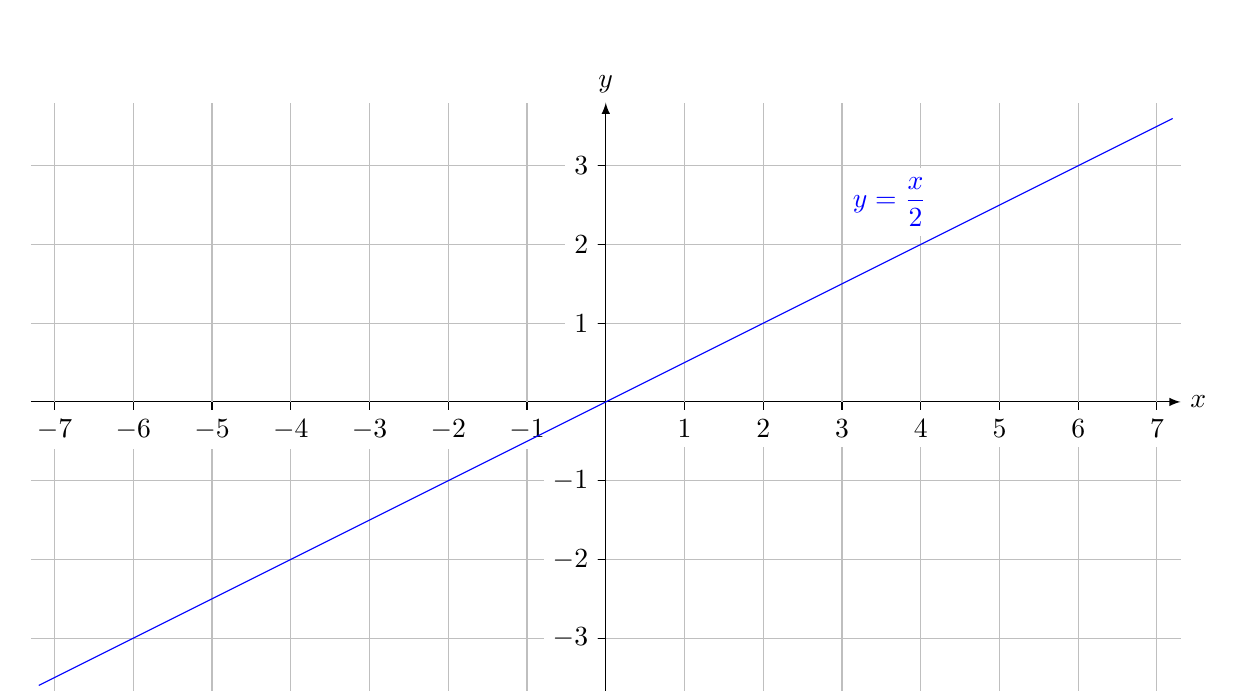
\begin{tikzpicture}
\draw[-latex] (-7.3, 0) -- (7.3, 0) node[right] {$x$} ;
\draw[-latex] (0, -3.8) -- (0, 3.8) node[above] {$y$} ;
\foreach \i in {-7,-6,-5,-4,-3,-2,-1,1,2,3,4,5,6,7} {
    \draw[lightgray] (\i, -3.8) -- (\i, 3.8) ;
    \draw (\i, 0) -- (\i, -0.1) node[below, fill=white] {$\i$} ;
}
\foreach \i in {-3,-2,-1,1,2,3} {
    \draw[lightgray] (-7.3, \i) -- (7.3, \i) ;
    \draw (0, \i) -- (-0.1, \i) node[left, fill=white] {$\i$} ;
}
\draw[blue] (-7.2, -3.6) -- (7.2, 3.6) ;
\draw[blue] (4.2, 2.1) node[above left, fill=white] {$y=\dfrac{x}{2}$} ;
\end{tikzpicture}}
\caption{Graph of the function $f : \mathbb{R} \to \mathbb{R}$ defined by $f(x) = \frac{x}{2}$ for all $x \in \mathbb{R}$}
\label{figGraphOfXOverTwo}
\end{figure}
\end{example}

\begin{exercise}
Find a function $f : \mathbb{Z} \to \mathbb{Z}$ whose graph is equal to the set
\[ \{ \dots, ({-2}, {-5}), ({-1}, {-2}), (0, 1), (1, 4), (2, 7), (3, 10), \dots \} \]
\end{exercise}

\Cref{thmFunctionsAsGraphs} below provides a way of verifying that a function is well-defined by characterising their graphs.

\begin{theorem}
\label{thmFunctionsAsGraphs}
Let $X$ and $Y$ be sets. A subset $G \subseteq X \times Y$ is the graph of a function if and only if
\[ \forall x \in X,\, \exists ! y \in Y,\, (x,y) \in G \]
\end{theorem}
\begin{cproof}
($\Rightarrow$). Suppose $G \subseteq X \times Y$ is the graph of a function, say $G = \mathrm{Gr}(f)$ for some $f : X \to Y$. Then for each $x \in X$, it follows from well-definedness of $f$ that $f(x)$ is the unique element $y \in Y$ for which $(x, y) \in G$. That is, $(x,f(x)) \in G$, and if $y \in Y$ with $(x,y) \in G$, then $y=f(x)$.

($\Leftarrow$). Suppose $G \subseteq X \times Y$ satisfies $\forall x \in X,\, \exists ! y \in Y,\, (x,y) \in G$. Define a function $f : X \to Y$ by, for each $x \in X$, defining the value $f(x)$ to be the unique element $y \in Y$ for which $(x,y) \in G$. Well-definedness of $f$ is then immediate from our assumption of the existence and uniqueness of such a value of $y$ for each $x \in X$.
\end{cproof}

\begin{example}
The set $G$ defined by
\[ G = \{ (1, \mathsf{red}), (2, \mathsf{red}), (3, \mathsf{green}) \} \]
is the graph of a function $f : \{ 1, 2, 3 \} \to \{ \mathsf{red}, \mathsf{green}, \mathsf{blue} \}$. The function $f$ is defined by
\[ f(1) = \mathsf{red}, \quad f(2) = \mathsf{red}, \quad f(3) = \mathsf{green} \]
However, $G$ is \textit{not} the graph of a function $\{ 1, 2, 3, 4 \} \to \{ \mathsf{red}, \mathsf{green}, \mathsf{blue} \}$, since $G$ contains no elements of the form $(4,y)$ for $y \in \{ \mathsf{red}, \mathsf{green}, \mathsf{blue} \}$. Moreover, the set $G'$ defined by
\[ G' = \{ (1, \mathsf{red}), (2, \mathsf{red}), (2, \mathsf{blue}), (3, \mathsf{green}) \} \]
does not define the graph of a function $\{ 1, 2, 3 \} \to \{ \mathsf{red}, \mathsf{green}, \mathsf{blue} \}$, since there is not a \textit{unique} element of the form $(2,y)$ in $G'$---rather, there are two of them!
\end{example}

\begin{exercise}
For each of the following specifications of sets $X$, $Y$, $G$, determine whether or not $G$ is the graph of a function from $X$ to $Y$.
\begin{enumerate}[(a)]
\item $X = \mathbb{R}$, $Y = \mathbb{R}$, $G = \{ (a, a^2) \mid a \in \mathbb{R} \}$;
\item $X = \mathbb{R}$, $Y = \mathbb{R}$, $G = \{ (a^2, a) \mid a \in \mathbb{R} \}$;
\item $X = \mathbb{R}^{\ge 0}$, $Y = \mathbb{R}^{\ge 0}$, $G = \{ (a^2, a) \mid a \in \mathbb{R}^{\ge 0} \}$, where $\mathbb{R}^{\ge 0} = \{ x \in \mathbb{R} \mid x \ge 0 \}$;
\item $X = \mathbb{Q}$, $Y = \mathbb{Q}$, $G = \{ (x, y) \in \mathbb{Q} \times \mathbb{Q} \mid xy = 1 \}$.
\item $X = \mathbb{Q}$, $Y = \mathbb{Q}$, $G = \{ (a, a) \mid a \in \mathbb{Z} \}$;
\end{enumerate}
\end{exercise}

\begin{aside}
In light of \Cref{thmFunctionsAsGraphs}, some people choose to define functions $X \to Y$ as particular subsets of $X \times Y$---that is, they identify functions with their graphs. This is particularly useful when studying the logical foundations of mathematics. We avoid this practice here, because it is not conceptually necessary, and it would preclude other possible ways of encoding functions.
\end{aside}

We will now look at some more examples (and non-examples) of functions.

\begin{example} \label{exFirstExamplesOfFunctions}
\Cref{exEveryPositiveRealHasUniqueSquareRoot} gives a prime example of a function: it says that for every positive real number $a$ there is a unique positive real number $b$ such that $b^2=a$. This unique $b$ is precisely the positive square root $\sqrt{a}$ of $a$. Writing $\mathbb{R}^{>0}$ for the set of positive real numbers, we have thus established that taking the positive square root defines a function $\mathbb{R}^{>0} \to \mathbb{R}^{>0}$.
\end{example}

There is a class of functions called \textit{identity functions} that, despite being very simple, are so important that we will give them a numbered definition!

\begin{definition}
\label{defIdentityFunction}
\index{function!identity}
\index{identity function}
Let $X$ be a set. The \textbf{identity function} on $X$ is the function $\mathrm{id}_X : X \to X$\nindex{idX}{$\mathrm{id}_X$}{identity function} \inlatex{mathrm\{id\}\_X}\lindexmmc{mathrm}{$\mathrm{Aa}, \mathrm{Bb}, \dots$} defined by $\mathrm{id}_X(x)=x$ for all $x \in X$.
\end{definition}

You should convince yourself that the specification of $\mathrm{id}_X$ given in \Cref{defIdentityFunction} is well-defined.

Another interesting example of a function is the \textit{empty function}, which is useful in coming up with counterexamples and proving combinatorial identities (see \Cref{secCountingPrinciples}).

\begin{definition}
\label{defEmptyFunction}
\index{function!empty}
\index{empty function}
Let $X$ be a set. The \textbf{empty function} with codomain $X$ is the (unique!) function $\varnothing \to X$. It has no values, since there are no elements of its domain.
\end{definition}

Again, you should convince yourself that this specification is well-defined. Conceptually, convincing yourself of this is not easy; but writing down the proof of well-definedness is extremely easy---you will find that there is simply nothing to prove!

\begin{example}
Define $f : \mathbb{R} \to \mathbb{R}$ by the equation $f(x)^2=x$ for all $x \in \mathbb{R}$. This is not well-defined for a few reasons. First, if $x<0$ then there is no real number $y$ such that $y^2=x$, so for $x<0$ there are no possible values of $f(x)$ in the codomain of $f$, so \textit{existence} fails. Second, if $x>0$ then there are in fact \textit{two} real numbers $y$ such that $y^2=x$, namely the positive square root $\sqrt{x}$ and the negative square root $-\sqrt{x}$. The specification of $f$ does not indicate which of these values to take, so \textit{uniqueness} fails.

Notice that the function $r : \mathbb{R}^{>0} \to \mathbb{R}^{>0}$ from \Cref{exPositiveSquareRootFunction} \textit{is} (well-)defined by the equation $r(x)^2 = x$ for all $x \in \mathbb{R}^{>0}$. This illustrates why it is very important to specify the domain and codomain when defining a function.
\end{example}

\begin{exercise}
Which of the following specifications of functions are well-defined?
\begin{enumerate}[(a)]
\item $g : \mathbb{Q} \to \mathbb{Q}$ defined by the equation $(x+1)g(x)=1$ for all $x \in \mathbb{Q}$;
\item $h : \mathbb{N} \to \mathbb{Q}$ defined by $(x+1)h(x)=1$ for all $x \in \mathbb{N}$;
\item $k : \mathbb{N} \to \mathbb{N}$ defined by $(x+1)k(x)=1$ for all $x \in \mathbb{N}$;
\item $\ell : \mathbb{N} \to \mathbb{N}$ defined by $\ell(x)=\ell(x)$ for all $x \in \mathbb{N}$.
\end{enumerate}
\end{exercise}

\begin{exercise}
\label{exWellDefinednessOfFunctionOnUnion}
Find a condition on sets $X$ and $Y$ such that the specification of a function $i : X \cup Y \to \{ 0, 1 \}$ given by
\[ i(z) = \begin{cases} 0 & \text{if } z \in X \\ 1 & \text{if } z \in Y \end{cases} \]
to be well-defined.
\begin{backhint}
\hintref{exWellDefinednessOfFunctionOnUnion}
What is the value of $i(z)$ if $z \in X \cap Y$?
\end{backhint}
\end{exercise}

\subsection*{Composition of functions}

In our section on sets, we talked about various operations that can be performed on sets---union, intersection, and so on. There are also operations on functions, by far the most important of which is \textit{composition}. To understand how composition works, let's revisit the algorithmically defined function $M : \mathbb{Q} \to \mathbb{Q}$ from page \pageref{txtAlgorithmicallyDefinedFunctionExample}:
\begin{center}
multiply by $2$ $\to$ add $5$ $\to$ square the result $\to$ divide by $6$
\end{center}
The function $M$ is, in some sense, a \textit{sequence} of functions, performed one-by-one until the desired result is reached. This is precisely \textit{composition of functions}.

\begin{definition}
\label{defComposition} \label{defComposite}
Given functions $f : X \to Y$ and $g : Y \to Z$, their \textbf{composite} $g \circ f$\nindex{composition}{$\circ$}{composition} \inlatexnb{g \textbackslash{}circ f}\lindexmmc{circ}{$\circ$} (read `$g$ composed with $f$' or `$g$ after $f$' or even just `$g$ $f$') is the function $g \circ f : X \to Z$ defined by
\[ (g \circ f)(x) = g(f(x)) \text{ for all } x \in X \]
\end{definition}
Intuitively, $g \circ f$ is the function resulting from first applying $f$, and then applying $g$, to the given input.

\begin{commonerror}
Function composition is in some sense written `backwards': in the expression $g \circ f$, the function which is applied \textit{first} is written \textit{last}---there is a good reason for this: the argument to the function is written after the function! However, this mis-match often trips students up on their first exposure to function composition, so be careful!
\end{commonerror}

\begin{example}
\label{exDecompositionOfFunctionQToQ}
The function $M$ from page \pageref{txtAlgorithmicallyDefinedFunctionExample} can be defined as the composite
\[ M = ((k \circ h) \circ g) \circ f \]
where
\begin{itemize}
\item $f : \mathbb{Q} \to \mathbb{Q}$ is defined by $f(x)=2x$ for all $x \in \mathbb{Q}$;
\item $g : \mathbb{Q} \to \mathbb{Q}$ is defined by $g(x)=x+5$ for all $x \in \mathbb{Q}$;
\item $h : \mathbb{Q} \to \mathbb{Q}$ is defined by $h(x)=x^2$ for all $x \in \mathbb{Q}$;
\item $k : \mathbb{Q} \to \mathbb{Q}$ is defined by $k(x)=\frac{x}{6}$ for all $x \in \mathbb{Q}$.
\end{itemize}
\end{example}

\begin{exercise}
Let $f,g,h,k : \mathbb{Q} \to \mathbb{Q}$ be as in \Cref{exDecompositionOfFunctionQToQ}. Compute equations defining the following composites:
\begin{enumerate}[(a)]
\item $f \circ g$;
\item $g \circ f$;
\item $((f \circ g) \circ h) \circ k$;
\item $f \circ (g \circ (h \circ k))$;
\item $(g \circ g) \circ (g \circ g)$.
\end{enumerate}
\end{exercise}

\begin{example}
\label{exCompositionWithIdentityIsTrivial}
Let $f : X \to Y$ be any function. Then
\[ \mathrm{id}_Y \circ f = f = f \circ \mathrm{id}_X \]
To see this, let $x \in X$. Then
\begin{align*}
(\mathrm{id}_Y \circ f)(x) &= \mathrm{id}_Y(f(x)) && \text{by definition of composition} \\
&= f(x) && \text{by definition of $\mathrm{id}_Y$} \\
&= f(\mathrm{id}_X(x)) && \text{by definition of $\mathrm{id}_X$} \\
&= (f \circ \mathrm{id}_X)(x) && \text{by definition of composition}
\end{align*}
Equality of the three functions in question follows.
\end{example}

\begin{exercise}
\label{exCompositionIsAssociative}
Prove that composition of functions is \textit{associative}, that is, if $f : X \to Y$, $g : Y \to Z$ and $h : Z \to W$ are functions, then
\[ h \circ (g \circ f) = (h \circ g) \circ f : X \to W \]
As a consequence of associativity, when we want to compose more than two functions, it doesn't matter what order we compose the functions in. As such, we can just write $h \circ g \circ f$.
\end{exercise}

\begin{exercise}
\label{exCompositionWithoutMatchingCodomains}
Let $f : X \to Y$ and $g : Z \to W$ be functions, and suppose that $Y \subsetneqq Z$. Note that there is a function $h : X \to W$ defined by $h(x)=g(f(x))$ for all $x \in X$. Write $h$ as a composite of functions involving $f$ and $g$.
\begin{backhint}
\hintref{exCompositionWithoutMatchingCodomains}
Look closely at \Cref{defComposition}.
\end{backhint}
\end{exercise}

\subsection*{Characteristic functions}

A class of functions that are particularly useful for proving results about sets are \textit{characteristic functions}.

\begin{definition}
\label{defCharacteristicFunction}
\index{characteristic function}
\index{function!characteristic}
Let $X$ be a set and let $U \subseteq X$. The \textbf{characteristic function} of $U$ in $X$ is the function $\chi_U : X \to \{ 0,1 \}$ \inlatex{chi\_\{U\}} defined by
\[ \chi_U(a) = \begin{cases} 1 & \text{if } a \in U \\ 0 & \text{if } a \not\in U \end{cases} \]
\end{definition}

\begin{example}
Consider the subset $U = \{ 1,3,5 \} \subseteq [6]$. Then the values of the characteristic function $\chi_U : [6] \to \{0,1\}$ are given by
\[ \begin{matrix} \chi_U(1) = 1 & \chi_U(2) = 0 & \chi_U(3) = 1 \\ \chi_U(4) = 0 & \chi_U(5) = 1 & \chi_U(6) = 0 \end{matrix} \]
\end{example}

\begin{theorem}
\label{thmCharacteristicFunctionsCharacteriseSubsets}
Let $X$ be a set and let $U, V \subseteq X$. Then $U=V$ if and only if $\chi_U = \chi_V$.
\end{theorem}

\begin{cproof}
\fixlistskip
\begin{itemize}
\item ($\subseteq$)
%% BEGIN EXTRACT (xtrAssumeExample) %%
Assume $U=V$ and let $a \in X$. Then
\begin{align*}
\chi_U(a) = 1 & \Leftrightarrow a \in U && \text{by definition of $\chi_U$} \\
&\Leftrightarrow a \in V && \text{since $U=V$} \\
&\Leftrightarrow \chi_V(a) = 1 && \text{by definition of $\chi_V$}
\end{align*}
%% END EXTRACT %%
Likewise $\chi_U(a) = 0$ if and only if $\chi_V(a) = 1$, so that $\chi_U = \chi_V$ by function extensionality.

\item ($\supseteq$) Assume $\chi_U = \chi_V$ and let $a \in X$. Then
\begin{align*}
a \in U & \Leftrightarrow \chi_U(a) = 1 && \text{by definition of $\chi_U$} \\
&\Leftrightarrow \chi_V(a) = 1 && \text{since $\chi_U = \chi_V$} \\
&\Leftrightarrow a \in V && \text{by definition of $\chi_V$}
\end{align*}
so $U=V$ by set extensionality.
\end{itemize}
\end{cproof}

\begin{strategy}[Proving set identities using characteristic functions]
\label{strSetIdentitiesFromCharacteristicFunctions}
In order to prove that two subsets $U$ and $V$ of a set $X$ are equal, it suffices to prove that $\chi_U = \chi_V$.
\end{strategy}

\begin{theorem}
\label{thmSetIdentitiesFromCharacteristicFunctions}
Let $X$ be a set and let $U,V \subseteq X$. Then
\begin{enumerate}[(a)]
\item $\chi_{U \cap V}(a) = \chi_U(a) \chi_V(a)$ for all $a \in X$;
\item $\chi_{U \cup V}(a) = \chi_U(a) + \chi_V(a) - \chi_U(a)\chi_V(a)$ for all $a \in X$;
\item $\chi_{X \setminus U}(a) = 1 - \chi_U(a)$ for all $a \in X$.
\end{enumerate}
\end{theorem}

\begin{cproof}[of {(a)}]
Let $a \in X$. Since the only values that $\chi_U(a)$ and $\chi_V(a)$ can take are $0$ and $1$, we have
\[ \chi_U(a) \chi_V(a) = \begin{cases} 1 & \text{if $\chi_U(a) = 1$ and $\chi_V(a) = 1$} \\ 0 & \text{otherwise} \end{cases} \]
But $\chi_U(a) = 1$ if and only if $a \in U$ and $\chi_V(a) = 1$ if and only if $a \in V$, so that
\[ \chi_U(a) \chi_V(a) = \begin{cases} 1 & \text{if $a \in U \cap V$} \\ 0 & \text{if $a \not\in U \cap V$} \end{cases} \]
This is exactly to say that $\chi_U(a) \chi_V(a) = \chi_{U \cap V}(a)$, as required.
\end{cproof}

\begin{exercise}
Prove parts (b) and (c) of \Cref{thmSetIdentitiesFromCharacteristicFunctions}.
\end{exercise}

\Cref{thmSetIdentitiesFromCharacteristicFunctions} can be used in conjunction with \Cref{strSetIdentitiesFromCharacteristicFunctions} to prove set theoretic identities using their characteristic functions.

\begin{example}
In \Cref{exIntersectionDistributesOverUnion} we proved that $X \cap (Y \cup Z) = (X \cap Y) \cup (X \cap Z)$ for all sets $X$, $Y$ and $Z$. We prove this again using characteristic functions, considering $X$, $Y$ and $Z$ as subsets of a universal set $\mathcal{U}$.

So let $a \in U$. Then
\begin{align*}
& \chi_{X \cap (Y \cup Z)}(a) && \\
&= \chi_X(a) \chi_{Y \cup Z}(a) && \text{by \Cref{thmSetIdentitiesFromCharacteristicFunctions}(a)} \\
&= \chi_X(a) (\chi_Y(a) + \chi_Z(a) - \chi_Y(a)\chi_Z(a)) && \text{by \Cref{thmSetIdentitiesFromCharacteristicFunctions}(b)} \\
&= \chi_X(a)\chi_Y(a) + \chi_X(a)\chi_Z(a) - \chi_X(a)\chi_Y(a)\chi_Z(a) && \text{rearranging} \\
&= \chi_X(a)\chi_Y(a) + \chi_X(a)\chi_Z(a) - \chi_X(a)^2\chi_Y(a)\chi_Z(a) && \text{since $\chi_X(a)^2=\chi_X(a)$} \\
&= \chi_{X \cap Y}(a) + \chi_{X \cap Z}(a) - \chi_{X \cap Y}(a) \chi_{X \cap Z}(a) && \text{by \Cref{thmSetIdentitiesFromCharacteristicFunctions}(a)} \\
&= \chi_{(X \cap Y) \cup (X \cap Z)}(a) && \text{by \Cref{thmSetIdentitiesFromCharacteristicFunctions}(b)}
\end{align*}
Using \Cref{strSetIdentitiesFromCharacteristicFunctions}, it follows that $X \cap (Y \cup Z) = (X \cap Y) \cup (X \cap Z)$.
\end{example}

\begin{exercise}
Use characteristic functions to prove de Morgan's laws for pairwise unions and intersections (\Cref{thmDeMorganForSets}).
\end{exercise}

\subsection*{Images and preimages}

\begin{definition}
\label{defImage}
Let $f : X \to Y$ be a function and let $U \subseteq X$. The \textbf{image of} $U$ \textbf{under} $f$ is the subset $f[U] \subseteq Y$\nindex{functionImage}{$f[U]$}{image} (also written $f_*(U)$ \inlatexnb{f\_*} or even just $f(U)$) is defined by
\[ f[U] = \{ f(x) \mid x \in U \} = \{ y \in Y \mid \exists x \in U,\, y = f(x) \} \]
That is, $f[U]$ is the set of values that the function $f$ takes when given inputs from $U$.

The \textbf{image of} $f$ is the image of the entire domain, i.e.\ the set $f[X]$.
\end{definition}

\begin{example}
Let $f : \mathbb{R} \to \mathbb{R}$ be defined by $f(x)=x^2$. The image of $f$ is the set $\mathbb{R}^{\ge 0}$ of all nonnegative real numbers. Let's prove this:
\begin{itemize}
\item ($f[\mathbb{R}] \subseteq \mathbb{R}^{\ge 0}$). Let $y \in f[\mathbb{R}]$. Then $y=x^2$ for some $x \in \mathbb{R}$. But $x^2 \ge 0$, so we must have $y \in \mathbb{R}^{\ge 0}$, as required.
\item ($\mathbb{R}^{\ge 0} \subseteq f[\mathbb{R}]$). Let $y \in \mathbb{R}^{\ge 0}$. Then $\sqrt{y} \in \mathbb{R}$, and $y = (\sqrt{y})^2 = f(\sqrt{y})$. Hence $y \in f[\mathbb{R}]$, as required.
\end{itemize}
We have shown by double containment that $f[\mathbb{R}] = \mathbb{R}^{\ge 0}$.
\end{example}

\begin{exercise}
For each of the following functions $f$ and subsets $U$ of their domain, describe the image $f[U]$.
\begin{enumerate}[(a)]
\item $f : \mathbb{Z} \to \mathbb{Z}$ defined by $f(n)=3n$, with $U = \mathbb{N}$;
\item $f : X \to X \times X$ (where $X$ is any set) defined by $f(x)=(x,x)$ with $U=X$;
\item $f : \{ a, b, c \} \to \{ 1, 2, 3 \}$ defined by $f(a)=1$, $f(b)=3$ and $f(c)=1$, with $U=\{a,b,c\}$.
\end{enumerate}
\end{exercise}

\begin{exercise}
Prove that $f[\varnothing] = \varnothing$ for all functions $f$.
\end{exercise}

\begin{example}
\label{exImageOfIntersectionSubsetIntersectionOfImage}
Let $f : X \to Y$ be a function and let $U, V \subseteq X$. Then $f[U \cap V] \subseteq f[U] \cap f[V]$. To see this, let $y \in f[U \cap V]$. Then $y = f(x)$ for some $x \in U \cap V$. By definition of intersection, $x \in U$ and $x \in V$. Since $x \in U$ and $y=f(x)$, we have $y \in f[U]$; likewise, since $x \in V$, we have $y \in f[V]$. But then by definition of intersection, we have $y \in f[U] \cap f[V]$.
\end{example}

\begin{exercise}
Let $f : X \to Y$ be a function and let $U, V \subseteq X$. We saw in \Cref{exImageOfIntersectionSubsetIntersectionOfImage} that $f[U \cap V] \subseteq f[U] \cap f[V]$. Determine which of the following is true, and for each, provide a proof of its truth or falsity:
\begin{enumerate}[(a)]
\item $f[U] \cap f[V] \subseteq f[U \cap V]$;
\item $f[U \cup V] \subseteq f[U] \cup f[V]$;
\item $f[U] \cup f[V] \subseteq f[U \cup V]$.
\end{enumerate}
\end{exercise}

\begin{definition}
\label{defPreimage}
Let $f : X \to Y$ be a function and let $V \subseteq Y$. The \textbf{preimage of} $V$ \textbf{under} $f$ is the subset $f^{-1}[V]$\nindex{functionPreImage}{$f^{-1}[V]$}{preimage} \inlatexnb{f\^{}\{-1\}} (also written $f^*(V)$ \inlatexnb{f\^{}*}, or just $f^{-1}(V)$) is defined by
\[ f^{-1}[V] = \{ x \in X \mid f(x) \in V \} = \{ x \in X \mid \exists y \in V,\, f(x) = y \} \]
That is, $f^{-1}[V]$ is the set of all the elements of its domain $X$ that the function $f$ sends to elements of $V$.
\end{definition}

\begin{example}
Let $f : \mathbb{Z} \to \mathbb{Z}$ be the function defined by $f(x)=x^2$ for all $x \in X$. Then
\begin{itemize}
\item $f^{-1}[ \{ 1, 4, 9 \} ] = \{ -3, -2, -1, 1, 2, 3 \}$;
\item $f^{-1}[ \{ 1, 2, 3, 4, 5, 6, 7, 8, 9 \} ] =  \{ -3, -2, -1, 1, 2, 3 \}$ too, since the other elements of $[9]$ are not perfect squares, and hence not of the form $f(x)$ for $x \in \mathbb{Z}$;
\item $f^{-1}[\mathbb{N}] = \mathbb{Z}$, since for any $x \in \mathbb{Z}$ we have $f(x) \ge 0$, so that $f(x) \in \mathbb{N}$.
\end{itemize}
\end{example}

\begin{example}
Let $f : X \to Y$ be a function, let $U \subseteq X$ and let $V \subseteq Y$. Then $f[U] \subseteq V$ if and only if $U \subseteq f^{-1}[V]$. The proof is as follows.

($\Rightarrow$). Suppose $f[U] \subseteq V$; we'll prove $U \subseteq f^{-1}[V]$. So fix $x \in U$. Then $f(x) \in f[U]$ by definition of image. But then $f(x) \in V$ by our assumption that $f[U] \subseteq V$, and so $x \in f^{-1}[V]$ by definition of preimage. Since $x$ was arbitrarily chosen from $U$, it follows that $U \subseteq f^{-1}[V]$.

($\Leftarrow$). Suppose $U \subseteq f^{-1}[V]$; we'll prove $f[U] \subseteq V$. So fix $y \in f[U]$. Then $y=f(x)$ for some $x \in U$ by definition of image. But then $x \in f^{-1}[V]$ by our assumption that $U \subseteq f^{-1}[V]$, and so $f(x) \in V$ by definition of preimage. But $y=f(x)$, so $y \in V$, and since $y$ was arbitrarily chosen, it follows that $f[U] \subseteq V$.
\end{example}

The following exercise demonstrates that preimages interact very nicely with the basic set operations (intersection, union and relative complement):
\begin{exercise}
Let $f : X \to Y$ be a function and let $U, V \subseteq Y$. Prove that:
\begin{enumerate}[(a)]
\item $f^{-1}[U \cap V] = f^{-1}[U] \cap f^{-1}[V]$;
\item $f^{-1}[U \cup V] = f^{-1}[U] \cup f^{-1}[V]$; and
\item $f^{-1}[Y \setminus U] = X \setminus f^{-1}[U]$.
\end{enumerate}
\end{exercise}

\begin{exercise}
Let $f : X \to Y$ be a function. Prove that $f^{-1}[\varnothing] = \varnothing$ and $f^{-1}[Y]=X$.
\end{exercise}

\begin{exercise}
Let $f : X \to Y$ be a function. Provide a proof of the truth or falsity of each of the following statements:
\begin{enumerate}[(a)]
\item $U \subseteq f^{-1}[f[U]]$ for all $U \subseteq X$;
\item $f^{-1}[f[U]] \subseteq U$ for all $U \subseteq X$;
\item $V \subseteq f[f^{-1}[V]]$ for all $V \subseteq Y$;
\item $f[f^{-1}[V]] \subseteq V$ for all $V \subseteq Y$.
\end{enumerate}
\end{exercise}

\begin{exercise}
\label{exCharacteristicFunctionsCorrespondWithSubsets}
Let $X$ be a set. Prove that every function $f : X \to \{0,1\}$ is the characteristic function of the subset $f^{-1}[\{1\}] \subseteq X$.
\end{exercise}

\index{function|)}

\newpage
\section{Injections and surjections}
\secbegin{secInjectionsSurjections}
\index{injection|(}
\index{surjection|(}
\index{bijection|(}

To motivate some of the definitions to come, look at the dots ($\bullet$) and stars ($\star$) below. Are there more dots or more stars?
\begin{center}
\fitwidth{\begin{tikzpicture}
\foreach \x in {1,2,3,4,5,6,7,8,9,10,11,12,13,14,15,16,17,18,19}
  \node at (0.75*\x, 0.75) {$\bullet$};

\foreach \x in {1,2,3,4,5,6,7,8,9,10,11,12,13,14,15}
  \node at (0.75*\x, 0) {$\star$};
\end{tikzpicture}}
\end{center}

Pause for a second and think about how you knew the answer to this question.

Indeed, there are more dots than stars. There are a couple of ways to arrive at this conclusion:
\begin{enumerate}[(i)] 
\item You could count the number of dots, count the number of stars, and then compare the two numbers; or
\item You could notice that the dots and the stars are evenly spaced, but that the line of dots is longer than the line of stars.
\end{enumerate}
It is likely that you chose method (ii). In fact, it is likely that you haven't even counted the number of dots or the number of stars yet---and you don't need to! We can conclude that there are more dots than stars by simply pairing up dots with stars---we eventually run out of stars, and there are still dots left over, so there must have been more dots than stars.

\subsection*{Injectivity}

One way of formalising this act of pairing up stars with dots mathematically is to define a function $f : S \to D$ from the set $S$ of stars to the set $D$ of dots, where the value of $f$ at each star is the dot that it is paired with. We of course must do this in such a way that each dot is paired with at most one star:

\begin{center}
\fitwidth{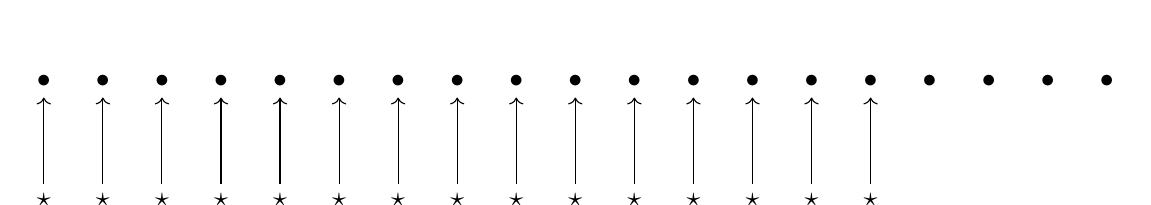
\begin{tikzpicture}
\foreach \x in {1,2,3,4,5,6,7,8,9,10,11,12,13,14,15,16,17,18,19}
  \node at (0.75*\x, 1.5) {$\bullet$};

\foreach \x in {1,2,3,4,5,6,7,8,9,10,11,12,13,14,15}
  \node at (0.75*\x, 0) {$\star$};

\foreach \x in {1,2,3,4,5,6,7,8,9,10,11,12,13,14,15}
  \draw [->] (0.75*\x, 0.2) -- (0.75*\x, 1.3);
\end{tikzpicture}}
\end{center}

It is a property of this function---called \textit{injectivity}---that allows us to deduce that there are more dots than stars.

Intuitively, a function $f : X \to Y$ is injective if it puts the elements of $X$ in one-to-one correspondence with the elements of a subset of $Y$---just like how the stars are in one-to-one correspondence with a subset of the dots in the example above.

\begin{definition}
\label{defInjective}\label{defInjection}
\index{function!injective (one-to-one)}
\index{injection}
A function $f : X \to Y$ is \textbf{injective} (or \textbf{one-to-one}) if
\[ \forall a,b \in X,\, f(a) = f(b) \Rightarrow a=b \]
An injective function is said to be an \textbf{injection}.
\end{definition}

\begin{strategy}[Proving a function is injective]
In order to prove that a function $f : X \to Y$ is injective, it suffices to fix $a,b \in X$, assume that $f(a)=f(b)$, and then derive $a=b$.
\end{strategy}

By contraposition, $f : X \to Y$ being injective is equivalent to saying, for all $a,b \in X$, if $a \ne b$, then $f(a) \ne f(b)$. This is usually less useful for \textit{proving} that a function is injective, but it does provide a good intuition---it says that $f$ sends distinct inputs to distinct outputs.

The following is a very simple example from elementary arithmetic:
\begin{example}
Define $f : \mathbb{Z} \to \mathbb{Z}$ by letting $f(x) = 2n+1$ for all $n \in \mathbb{Z}$. We'll prove that $f$ is injective. Fix $m, n \in \mathbb{Z}$, and assume that $f(m)=f(n)$. By definition of $f$, we have $2m+1=2n+1$. Subtracting $1$ yields $2m=2n$, and dividing by $2$ yields $m=n$. Hence $f$ is injective.
\end{example}

The following example is slightly more sophisticated.

\begin{proposition}
\label{propCompositeOfInjectionsIsInjection}
Let $f : X \to Y$ and $g : Y \to Z$ be functions. If $f$ and $g$ are injective, then $g \circ f$ is injective.
\end{proposition}
\begin{cproof}
Suppose that $f$ and $g$ are injective and
%% BEGIN EXTRACT (xtrVariableIntroductionExample) %%
let $a,b \in X$.
We need to prove that
\[ (g \circ f)(a) = (g \circ f)(b) \quad \Rightarrow \quad a=b \]
%% END EXTRACT %%
So assume $(g \circ f)(a) = (g \circ f)(b)$. By definition of function composition, this implies that $g(f(a))=g(f(b))$. By injectivity of $g$, we have $f(a)=f(b)$; and by injectivity of $f$, we have $a=b$.
\end{cproof}

\begin{exercise}
Let $f : X \to Y$ and $g : Y \to Z$ be functions. Prove that if $g \circ f$ is injective, then $f$ is injective.
\end{exercise}

\begin{exercise}
Write out what it means to say a function $f : X \to Y$ is \textit{not} injective, and say how you would prove that a given function is not injective. Give an example of a function which is not injective, and use your proof technique to write a proof that it is not injective.
\end{exercise}

\begin{exercise}
For each of the following functions, determine whether it is injective or not injective.
\begin{itemize} 
\item $f : \mathbb{N} \to \mathbb{Z}$, defined by $f(n)=n^2$ for all $n \in \mathbb{N}$.
\item $g : \mathbb{Z} \to \mathbb{N}$, defined by $g(n)=n^2$ for all $n \in \mathbb{Z}$.
\item $h : \mathbb{N} \times \mathbb{N} \times \mathbb{N} \to \mathbb{N}$, defined by $h(x,y,z) = 2^x \cdot 3^y \cdot 5^z$ for all $x,y,z \in \mathbb{N}$.
\end{itemize}
\end{exercise}

\begin{exercise}
\label{exLinearPolynomialIsInjective}
Let $a,b \in \mathbb{R}$ with $b \ne 0$, and define $f : \mathbb{R} \to \mathbb{R}$ by $f(t) = a+bt$ for all $t \in \mathbb{R}$. Prove that $f$ is injective.
\end{exercise}

\subsection*{Surjectivity}

Let's revisit the rows of dots and stars that we saw earlier.  Beforehand, we made our idea that there are more dots than stars formal by proving the existence of an injection $f : S \to D$ from the set $S$ of stars to the set $D$ of dots.

However, we could have drawn the same conclusion instead from defining a function $D \to S$, which in some sense \textit{covers} the stars with dots---that is, every star is paired up with at least one dot.

\begin{center}
\fitwidth{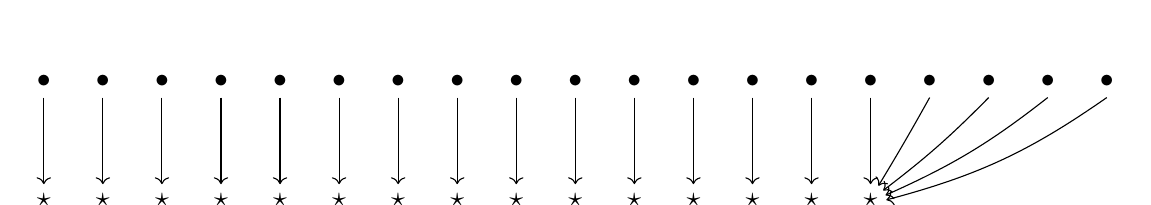
\begin{tikzpicture}
\foreach \x in {1,2,3,4,5,6,7,8,9,10,11,12,13,14,15,16,17,18,19}
  \node at (0.75*\x, 1.5) {$\bullet$};

\foreach \x in {1,2,3,4,5,6,7,8,9,10,11,12,13,14,15}
  \draw [->] (0.75*\x, 1.3) -- (0.75*\x, 0.2);

  \draw [->] (12, 1.3) to [bend left=1] (11.35, 0.18);
  \draw [->] (12.75, 1.3) to [bend left=4] (11.41, 0.12);
  \draw [->] (13.5, 1.3) to [bend left=7] (11.44, 0.06);
  \draw [->] (14.25, 1.3) to [bend left=10] (11.45, 0);

\foreach \x in {1,2,3,4,5,6,7,8,9,10,11,12,13,14,15}
  \node at (0.75*\x, 0) {$\star$};
\end{tikzpicture}}
\end{center}

This property is called \textit{surjectivity}---a function $f : X \to Y$ is surjective if every element of $Y$ is a value of $f$. This is made precise in \Cref{defSurjective}.

\begin{definition}
\label{defSurjective}\label{defSurjection}
A function $f : X \to Y$ is \textbf{surjective}\index{function!surjective}\index{surjection} (or \textbf{onto}) if
\[ \forall y \in Y,\ \exists x \in X,\ f(x) = y \]
A surjective function is said to be a \textbf{surjection}.
\end{definition}

\begin{strategy}
To prove that a function $f : X \to Y$ is surjective, it suffices to take an arbitrary element $y \in Y$ and, in terms of $y$, find an element $x \in X$ such that $f(x)=y$.

In order to find $x$, it is often useful to start from the equation $f(x)=y$ and derive some possible values of $x$. But be careful---in order to complete the proof, it is necessary to verify that the equation $f(x)=y$ is true for the chosen value of $x$.
\end{strategy}

\begin{example}
Fix $n \in \mathbb{N}$ with $n > 0$, and define a function $r : \mathbb{Z} \to \{ 0, 1, \dots, n-1 \}$ by letting $r(a)$ be the remainder of $a$ when divided by $n$ (see \Cref{thmDivisionPreliminary}). This function is surjective, since for each $k \in \{ 0, 1, \dots, n-1 \}$ we have $r(k)=k$.
\end{example}

\begin{exercise}
For each of the following pairs of sets $(X,Y)$, determine whether the function $f : X \to Y$ defined by $f(x)=2x+1$ is surjective.
\begin{enumerate}[(a)]
\item $X = \mathbb{Z}$ and $Y = \{ x \in \mathbb{Z} \mid x \text{ is odd} \}$;
\item $X = \mathbb{Z}$ and $Y = \mathbb{Z}$;
\item $X = \mathbb{Q}$ and $Y = \mathbb{Q}$;
\item $X = \mathbb{R}$ and $Y = \mathbb{R}$.
\end{enumerate}
\end{exercise}

\begin{exercise}
Let $f : X \to Y$ be a function. Find a subset $V \subseteq Y$ and a surjection $g : X \to V$ agreeing with $f$ (that is, such that $g(x)=f(x)$ for all $x \in X$).
\hintlabel{exSurjectiveCorestriction}{%
Recall \Cref{defImage}.
}
\end{exercise}

\begin{exercise}
Let $f : X \to Y$ be a function. Prove that $f$ is surjective if and only if $Y=f[X]$
\end{exercise}

\begin{exercise}
\label{exEpiMonoFactorisation}
Let $f : X \to Y$ be a function. Prove that there is a set $Z$ and functions
\[ p : X \to Z \quad \text{and} \quad i : Z \to Y \]
such that $p$ is surjective, $i$ is injective, and $f = i \circ p$.
\begin{backhint}
\hintref{exEpiMonoFactorisation}
If $Z$ were a subset of $Y$, then we could easily define an injection $i : Z \to Y$ by $i(z)=z$ for all $z \in Z$. Are there any subsets of $Y$ that are associated with a function whose codomain is $Y$?
\end{backhint}
\end{exercise}

\begin{exercise}
Let $f : X \to \mathcal{P}(X)$ be a function. By considering the set $B = \{ x \in X \mid x \not\in f(x) \}$, prove that $f$ is not surjective.
\hintlabel{exRussellSubset}{%
Note that $B \in \mathcal{P}(X)$. Prove that there does not exist $a \in X$ such that $B = f(a)$.
}
\end{exercise}

\subsection*{Bijectivity}

Bijective functions formalise the idea of putting sets into one-to-one correspondence---each element of one set is paired with exactly one element of another.

\begin{definition}
\label{defBijective}\label{defBijection}
A function $f : X \to Y$ is \textbf{bijective}\index{function!bijective} if it is injective and surjective. A bijective function is said to be a \textbf{bijection}\index{bijection}.
\end{definition}

\begin{prooftip}
To prove that a function $f$ is bijective, prove that it is injective and surjective.
\end{prooftip}

\begin{example}
\label{exDyadicRationalsBijection}
Let $D \subseteq \mathbb{Q}$ be the set of \textit{dyadic rational numbers}, that is
\[ D = \left\{ x \in \mathbb{Q} \ \bigg|\  x = \frac{a}{2^n} \text{ for some } a \in \mathbb{Z} \text{ and } n \in \mathbb{N} \right\} \]
Let $k \in \mathbb{N}$, and define $f : D \to D$ by $f(x)=\frac{x}{2^k}$. We will prove that $f$ is a bijection.
\begin{itemize}
\item (\textbf{Injectivity}) Fix $x,y \in D$ and suppose that $f(x)=f(y)$. Then $\frac{x}{2^k}=\frac{y}{2^k}$, so that $x=y$, as required.
\item (\textbf{Surjectivity}) Fix $y \in D$. We need to find $x \in D$ such that $f(x)=y$. Well certainly if $2^ky \in D$ then we have \[ f(2^ky)=\frac{2^ky}{2^k}=y \]
so it suffices to prove that $2^ky \in D$.
%% BEGIN EXTRACT (xtrCasesExample)
Since $y \in D$, we must have $y=\frac{a}{2^n}$ for some $n \in \mathbb{N}$.
\begin{itemize}
\item If $k \le n$ then $n-k \in \mathbb{N}$ and so $2^ky=\frac{a}{2^{n-k}} \in D$.
\item If $k > n$ then $k-n>0$ and $2^ky = 2^{k-n}a \in \mathbb{Z}$; but $\mathbb{Z} \subseteq D$ since if $a \in \mathbb{Z}$ then $a=\frac{a}{2^0}$. So again we have $2^ky \in D$.
\end{itemize}
In both cases we have $2^ky \in D$; and $f(2^ky)=y$, so that $f$ is surjective.
%% END EXTRACT
\end{itemize}
Since $f$ is both injective and surjective, it is bijective.
\end{example}

\begin{exercise}
\label{exIdentityBijection}
Let $X$ be a set. Prove that the identity function $\mathrm{id}_X : X \to X$ is a bijection.
\end{exercise}

\begin{exercise}
Let $n \in \mathbb{N}$ and let $\{ X_k \mid 1 \le k \le n \}$ be a family of sets. Prove by induction on $n$ that there is a bijection $\displaystyle \prod_{k=1}^{n+1} X_k \to \left( \prod_{k=1}^n X_k \right) \times X_n$.
\hintlabel{exProductOfSuccNSets}{%
To define the bijection, think about what the elements of the two sets look like: The elements of $\prod_{k=1}^{n+1} X_k$ look like $(a_1, a_2, \dots, a_n, a_{n+1})$, where $a_k \in X_k$ for each $1 \le k \le n+1$. On the other hand, the elements of $\left( \prod_{k=1}^n X_k \right) \times X_{n+1}$ look like $((a_1, a_2, \dots, a_n), a_{n+1})$.
}
\end{exercise}

\begin{exercise}
\label{exCompositeOfBijectionsIsBijection}
Let $f : X \to Y$ and $g : Y \to Z$ be bijections. Prove that $g \circ f$ is a bijection.
\end{exercise}

\subsection*{Inverses}

Our next goal is to characterise injections, surjections and bijections in terms of other functions, called \textit{inverses}.

Recall \Cref{defInjection}, which says that a function $f : X \to Y$ is injective if, for all $a,b \in X$, if $f(a)=f(b)$ then $a=b$.

\begin{exercise}
Let $f : X \to Y$ be a function. Prove that $f$ is injective if and only if
\[ \forall y \in f[X],\, \exists ! x \in X,\, y=f(x) \]
\end{exercise}

Thinking back to \Cref{secFunctions}, you might notice that this means that the logical formula `$y=f(x)$' defines a function $f[X] \to X$---specifically, if $f$ is injective then there is a function $g : f[X] \to X$ which is (well-)defined by specifying $x=g(f(x))$ for all $x \in X$. Thinking of $f$ as an \textit{encoding} function, we then have that $g$ is the corresponding \textit{decoding} function---decoding is possible by injectivity of $f$. (If $f$ were not injective then distinct elements of $X$ might have the same encoding, in which case we're stuck if we try to decode them!)

\begin{exercise}
\label{exEncodingPairs}
Define a function $e : \mathbb{N} \times \mathbb{N} \to \mathbb{N}$ by $e(m,n) = 2^m \cdot 3^n$. Prove that $e$ is injective. We can think of $e$ as encoding \textit{pairs} of natural numbers as single natural numbers---for example, the pair $(4,1)$ is encoded as $2^4 \cdot 3^1 = 48$. For each of the following natural numbers $k$, find the pairs of natural numbers encoded by $e$ as $k$:
\[ 1 \qquad 24 \qquad 7776 \qquad 59049 \qquad 396718580736 \]
\end{exercise}

In \Cref{exEncodingPairs}, we were able to decode any natural number of the form $2^m \cdot 3^n$ for $m,n \in \mathbb{N}$. This process of decoding yields a function
\[ d : \{ k \in \mathbb{N} \mid k=2^m \cdot 3^n \text{ for some } m,n \in \mathbb{N} \} \to \mathbb{N} \times \mathbb{N} \]
What would happen if we tried to decode a natural number not of the form $2^m \cdot 3^n$ for $m,n \in \mathbb{N}$, say $5$ or $100$? Well\dots{} it doesn't really matter! All we need to be true is that $d(e(m,n))=(m,n)$ for all $(m,n) \in \mathbb{N} \times \mathbb{N}$; the value of $d$ on other natural numbers is irrelevant.

\begin{definition}
\label{defLeftInverse}
\index{inverse!left inverse}
\index{left inverse}
Let $f : X \to Y$ be a function. A \textbf{left inverse} (or \textbf{post-inverse}) for $f$ is a function $g : Y \to X$ such that $g \circ f = \mathrm{id}_X$.
\end{definition}

\begin{example}
Let $e : \mathbb{N} \times \mathbb{N} \to \mathbb{N}$ be as in \Cref{exEncodingPairs}. Define a function $d : \mathbb{N} \to \mathbb{N} \times \mathbb{N}$ by
\[ d(k) = \begin{cases}
(m,n) & \text{if } k=2^m \cdot 3^n \text{ for some } m,n \in \mathbb{N} \\
(0,0) & \text{otherwise}
\end{cases} \]
Note that $d$ is well-defined by the fundamental theorem of arithmetic (\Cref{thmFTA}). Moreover, given $m,n \in \mathbb{N}$, we have
\[ d(e(m,n)) = d(2^m \cdot 3^n) = (m,n) \]
and so $d$ is a left inverse for $e$.
\end{example}

\begin{exercise}
\label{exIfHasLeftInverseThenInjective}
Let $f : X \to Y$ be a function. Prove that if $f$ has a left inverse, then $f$ is injective.
\end{exercise}

\Cref{exIfHasLeftInverseThenInjective} gives us a new strategy for proving that a function is injective.

\begin{strategy}[Proving a function is injective by finding a left inverse]
In order to prove that a function $f : X \to Y$ is injective, it suffices to find a function $g : Y \to X$ such that $g(f(x)) = x$ for all $x \in X$.
\end{strategy}

It would be convenient if the converse to \Cref{exIfHasLeftInverseThenInjective} were true---and it is, provided that we impose the condition that the domain of the function be inhabited.

\begin{proposition}
\label{propIfInjectiveThenHasLeftInverse}
Let $f : X \to Y$ be a function. If $f$ is injective and $X$ is inhabited, then $f$ has a left inverse.
\end{proposition}

\begin{cproof}
Suppose that $f$ is injective and $X$ is inhabited. Fix $x_0 \in X$---note that this element exists since $X$ is inhabited---and define $g : Y \to X$ as follows.
\[ g(y) = \begin{cases} x & \text{if } y=f(x) \text{ for some } x \in X \\ x_0 & \text{otherwise} \end{cases} \]
The only part of the specification of $g$ that might cause it to fail to be well-defined is the case when $y=f(x)$ for some $x \in X$. The reason why $g$ is well-defined is precisely injectivity of $f$: if $y=f(x)$ for some $x \in X$, then the value of $x \in X$ for which $y = f(x)$ is unique. (Indeed, if $a \in X$ satisfied $y=f(a)$, then we'd have $a=x$ by injectivity of $f$.)

So $g$ is indeed well-defined. To see that $g$ is a left inverse for $f$, let $x \in X$. Letting $y = f(x)$, we see that $y$ falls into the first case in the specification of $g$, so that $g(f(x)) = g(y) = a$ for the value of $a \in X$ for which $y = f(a)$---but as noted above, we have $a=x$ by injectivity of $f$.
\end{cproof}

\begin{exercise}
Let $f : X \to Y$ be a function with left inverse $g : Y \to X$. Prove that $g$ is a surjection.
\hintlabel{exLeftInversesAreSurjective}{%
This can be proved in a single sentence; if you find yourself writing a long proof, then there is an easier way.
}
\end{exercise}

We established a relationship between injections and left inverses in \Cref{exIfHasLeftInverseThenInjective,propIfInjectiveThenHasLeftInverse}, so it might come as no surprise that there is a relationship between surjections and \textit{right} inverses.

\begin{definition}
\label{defRightInverse}
\index{inverse!right inverse}
\index{right inverse}
Let $f : X \to Y$ be a function. A \textbf{right inverse} (or \textbf{pre-inverse}) for $f$ is a function $g : Y \to X$ such that $f \circ g = \mathrm{id}_Y$.
\end{definition}

\begin{example}
Define $f : \mathbb{R} \to \mathbb{R}^{\ge 0}$ by $f(x)=x^2$. Note that $f$ is surjective, since for each $y \in \mathbb{R}^{\ge 0}$ we have $\sqrt{y} \in \mathbb{R}$ and $f(\sqrt{y}) = y$. However $f$ is not injective; for instance
\[ f(-1) = 1 = f(1) \]
Here are three right inverses for $f$:
\begin{itemize}
\item The positive square root function $g : \mathbb{R}^{\ge 0} \to \mathbb{R}$ defined by $g(y)=\sqrt{y}$ for all $y \in \mathbb{R}^{\ge 0}$. Indeed, for each $y \in \mathbb{R}^{\ge 0}$ we have
\[ f(g(y)) = f(\sqrt{y}) = (\sqrt{y})^2 = y \]
\item The negative square root function $h : \mathbb{R}^{\ge 0} \to \mathbb{R}$ defined by $h(y)=-\sqrt{y}$ for all $y \in \mathbb{R}^{\ge 0}$. Indeed, for each $y \in \mathbb{R}^{\ge 0}$ we have
\[ f(h(y)) = f(-\sqrt{y}) = (-\sqrt{y})^2 = y \]
\item The function $k : \mathbb{R}^{\ge 0} \to \mathbb{R}$ defined by
\[ k(y) = \begin{cases}
\sqrt{y} & \text{if } 2n \le y < 2n+1 \text{ for some } n \in \mathbb{N} \\
-\sqrt{y} & \text{otherwise}
\end{cases} \]
Note that $k$ is well-defined, and again $f(k(y)) = y$ for all $y \in \mathbb{R}^{\ge 0}$ since no matter what value $k(y)$ takes, it is equal to either $\sqrt{y}$ or $-\sqrt{y}$.
\end{itemize}
There are many more right inverses for $f$---in fact, there are infinitely many more!
\end{example}

\begin{exercise}
Let $f : X \to Y$ be a function. Prove that if $f$ has a right inverse, then $f$ is surjective.
\hintlabel{exIfHasRightInverseThenSurjective}{%
The proof is almost identical to \Cref{exLeftInversesAreSurjective}.
}
\end{exercise}

\begin{strategy}[Proving a function is surjective by finding a right inverse]
In order to prove that a function $f : X \to Y$ is surjective, it suffices to find a function $g : Y \to X$ such that $f(g(y)) = y$ for all $y \in Y$.
\end{strategy}

\subsection*{Interlude: the axiom of choice}

It would be convenient if the converse to \Cref{exIfHasRightInverseThenSurjective} were true---that is, if $f : X \to Y$ is surjective, then it has a right inverse. Let's examine what a proof of this fact would entail. The fact that $f : X \to Y$ is surjective can be expressed as
\[ \forall y \in Y,\, \exists x \in X,\, f(x) = y \]
A right inverse would be a function $g : Y \to X$, so by \Cref{defFunction}, it must satisfy the following condition
\[ \forall y \in Y,\, \exists ! x \in X,\, g(y) = x \]

The temptation is therefore to construct $g : Y \to X$ as follows. Let $y \in Y$. By definition of surjectivity, there exists some $x \in X$ such that $f(x) = y$---define $g(y)$ to be such an element $x$. Then we have $f(g(y)) = f(x) = y$, as required.

There is an extremely subtle---but important---issue with this construction.

By choosing $g(y)$ to be a fixed element of $X$ such that $f(x) = y$, we are assuming ahead of time that there is a mechanism for choosing, for each $y \in Y$, a unique element of $f^{-1}[\{y\}]$ to be the value of $g(y)$. In other words we are assuming that some statement $R(x,y)$ satisfies the property
\[ \forall y \in Y,\, \exists ! x \in X,\, [x \in f^{-1}[\{y\}] \wedge R(x,y)] \]
But by \Cref{defFunction}, this assumption is saying exactly that there exists a function $Y \to X$ that associates to each $y \in Y$ an element $x \in X$ such that $f(x) = y$.

To state this in plainer terms: we tried to prove that there exists a right inverse for $f$ by assuming that there exists a right inverse for $f$. Evidently, this is not a valid proof strategy.

Surprisingly, it turns out that neither the assumption that every surjection has a right inverse, nor the assumption that there exists a surjection with no right inverse, leads to a contradiction. As such, the assertion that every surjection has a right inverse is \textit{provably unprovable}, although the proof that it is unprovable is far beyond the scope of this textbook.

Nonetheless, the construction of a right inverse that we gave above didn't \textit{feel} like we were abusing the fabric of mathematics and logic.

The essence of the proof is that if a statement of the form $\forall a \in A,\, \exists b \in B,\, p(a,b)$ is true, then we should be able to define a function $h : A \to B$ such that $p(a,h(a))$ is true for all $a \in A$: the function $h$ `chooses' for each $a \in A$ a particular element $b = h(a) \in B$ such that $p(a,b)$ is true.

What makes this possible is to \textit{axiom of choice}, stated precisely below.

\begin{axiom}[Axiom of choice]
\label{axChoice}
\index{axiom of choice}
Let $\{ X_i \mid i \in I \}$ be a family of inhabited sets. Then there is a function $h : I \to \bigcup\limits_{i \in I} X_i$ such that $h(i) \in X_i$ for each $i \in I$.
\end{axiom}

There are reasons to keep track of the axiom of choice:
\begin{itemize}
\item The axiom of choice is perhaps the \textit{strangest} assumption that we make---most of the other axioms that we have stated have been `evidently true', but this is not the case for the axiom of choice;
\item There are fields of mathematics which require the translation of results about sets into results about other kinds of objects---knowing whether the axiom of choice is necessary to prove a result tells us whether this is possible;
\item The axiom of choice is highly non-constructive: if a proof of a result that does not use the axiom of choice is available, it usually provides more information than a proof of the same result that does use the axiom of choice.
\end{itemize}

With this in mind, when we need to invoke the axiom of choice to prove a result, we will mark the result with the letters {\small \textbf{AC}}. This can be freely ignored on first reading, but readers may find it useful when using this book as a reference at a later date.

\begin{propositionac}
\label{propUsingAC}
Let $X$ and $Y$ be sets and let $p(x,y)$ be a logical formula with free variables $x \in X$ and $y \in Y$. If $\forall x \in X,\, \forall y \in Y,\, p(x,y)$ is true, then there exists a function $h : X \to Y$ such that $\forall x \in X,\, p(x,h(x))$ is true.
\end{propositionac}

\begin{cproof}
For each $a \in X$, define $Y_a = \{ b \in Y \mid p(a,b) \}$. Note that $Y_a$ is inhabited for each $a \in X$ by the assumption that $\forall x \in X,\, \exists y \in Y,\, p(x,y)$ is true. Since $Y_a \subseteq Y$ for each $a \in X$, by the axiom of choice there exists a function $h : X \to Y$ such that $h(a) \in Y_a$ for all $a \in X$. But then $p(a,h(a))$ is true for each $a \in X$ by definition of the sets $Y_a$.
\end{cproof}

In light of \Cref{propUsingAC}, the axiom of choice manifests itself in proofs as the following proof strategy.

\begin{strategyac}[Making choices]
\label{strUsingAC}
If an assumption in a proof has the form $\forall x \in X,\, \exists y \in Y,\, p(x,y)$, then we may make a choice, for each $a \in A$, of a particular element $b = b_a \in B$ for which $p(a,b)$ is true.
\end{strategyac}

\subsection*{Back to inverses}

We now return to the converse of \Cref{exIfHasRightInverseThenSurjective}.

\begin{propositionac}
Every surjection has a right inverse.
\end{propositionac}

\begin{cproof}
Let $f : X \to Y$ be a surjection, and define $g : Y \to X$ as follows. Given $y \in Y$, define $g(y)$ to be a particular choice of $x \in X$ such that $f(x) = y$---note that there exists such an element $x \in X$ since $f$ is surjective, so $g$ exists by \Cref{strUsingAC}. But then by definition of $g$ we have $f(g(y)) = y$ for all $y \in Y$, so that $g$ is a surjection.
\end{cproof}

It seems logical that we might be able to classify bijections as being those functions which have a left inverse and a right inverse. We can actually say something stronger---the left and right inverse can be taken to be the same function! (In fact, \Cref{propLeftAndRightInversesAreEqual} establishes that they are necessarily the same function.)

\begin{definition}
\label{defInverse}
\index{inverse!two-sided}
\index{two-sided inverse}
Let $f : X \to Y$ be a function. A (\textbf{two-sided}) \textbf{inverse} for $f$ is a function $g : Y \to X$ which is both a left inverse and a right inverse for $f$.
\end{definition}

It is customary to simply say `inverse' rather than `two-sided inverse'.

\begin{example}
Let $D$ be the set of dyadic rational numbers, as defined in \Cref{exDyadicRationalsBijection}. There, we defined a function $f : D \to D$ defined by $f(x)=\frac{x}{2^k}$ for all $x \in D$, where $k$ is some fixed natural number. We find an inverse for $f$.

Define $g : D \to D$ by $g(x) = 2^kx$. Then
\begin{itemize}
\item $g$ is a left inverse for $f$. To see this, note that for all $x \in D$ we have
\[ g(f(x)) = g(\frac{x}{2^k}) = 2^k \cdot \frac{x}{2^k} = x \]
\item $g$ is a right inverse for $f$. To see this, note that for all $y \in D$ we have
\[ f(g(y)) = f(2^ky) = \frac{2^ky}{2^k} = y \]
\end{itemize}
Since $g$ is a left inverse for $f$ and a right inverse for $f$, it is a two-sided inverse for $f$.
\end{example}

\begin{exercise}
\label{exFindTwoSidedInverses}
The following functions have two-sided inverses. For each, find its inverse and prove that it is indeed an inverse.
\begin{enumerate}[(a)]
\item $f : \mathbb{R} \to \mathbb{R}$ defined by $f(x)=\frac{2x+1}{3}$.
\item $g : \mathcal{P}(\mathbb{N}) \to \mathcal{P}(\mathbb{N})$ defined by $g(X) = \mathbb{N} \setminus X$.
\item $h : \mathbb{N} \times \mathbb{N} \to \mathbb{N}$ defined by $h(m,n) = 2^m(2n+1)-1$ for all $m,n \in \mathbb{N}$.
\end{enumerate}
\begin{backhint}
\hintref{exFindTwoSidedInverses}
For part (c), don't try to write a formula for the inverse of $h$; instead, use the fundamental theorem of arithmetic.
\end{backhint}
\end{exercise}

In light of the correspondences between injections and left inverses, and surjections and right inverses, it may be unsurprising that there is a correspondence between \textit{bijections} and \textit{two-sided inverses}.

\begin{exercise}
\label{exBijectiveIffHasInverse}
Let $f : X \to Y$ be a function. Then $f$ is bijective if and only if $f$ has an inverse.
\end{exercise}

\begin{strategy}[Proving a function is bijective by finding an inverse]
In order to prove that a function $f : X \to Y$ is bijective, it suffices to find a function $g : Y \to X$ such that $g(f(x)) = x$ for all $x \in X$ and $f(g(y)) = y$ for all $y \in Y$.
\end{strategy}

When proving a function $f : X \to Y$ is bijective by finding an inverse $g : Y \to X$, it is important to check that $g$ is \textit{both} a left inverse \textit{and} a right inverse for $f$. If you only prove that $g$ is a left inverse for $f$, for example, then you have only proved that $f$ is injective!

It turns out that if a function has both a left and a right inverse, then they must be equal. This is the content of the following proposition.

\begin{proposition}
\label{propLeftAndRightInversesAreEqual}
Let $f : X \to Y$ be a function and suppose $\ell : Y \to X$ is a left inverse for $f$ and $r : Y \to X$ is a right inverse for $f$. Then $\ell=r$.
\end{proposition}
\begin{cproof}
The proof is deceptively simple:
\begin{align*}
\ell &= \ell \circ \mathrm{id}_Y && \text{by definition of identity functions} \\
&= \ell \circ (f \circ r) && \text{since $r$ is a right inverse for $f$} \\
&= (\ell \circ f) \circ r && \text{by \Cref{exCompositionIsAssociative}} \\
&= \mathrm{id}_X \circ r && \text{since $\ell$ is a left inverse for $f$} \\
&= r && \text{by definition of identity functions}
\end{align*}
\end{cproof}

There is some intuition behind why the left and right inverses of a function $f : X \to Y$ should be equal if they both exist.
\begin{itemize}
\item A left inverse $\ell : Y \to X$ exists only if $f$ is injective. It looks at each element $y \in Y$ and, if it is in the image of $f$, returns the (unique) value $x \in X$ for which $f(x)=y$.
\item A right inverse $r : Y \to X$ exists only if $f$ is surjective. It looks at each element $y \in Y$ and picks out one of the (possibly many) values $x \in X$ for which $f(x)=y$.
\end{itemize}
When $f$ is a bijection, every element of $Y$ is in the image of $f$ (by surjectivity), and is a value of $f$ at a unique element of $X$ (by injectivity), and so the left and right inverses are forced to return the same value on each input---hence they are equal.

It follows from \Cref{propLeftAndRightInversesAreEqual} that, for any function $f : X \to Y$, any two inverses for $f$ are equal---that is, every bijective function has a \textit{unique} inverse!

\begin{notation}
Let $f : X \to Y$ be a function. Write $f^{-1} : Y \to X$\nindex{functionInverse}{$f^{-1}$}{inverse function} to denote the (unique) inverse for $f$, if it exists.
\end{notation}

\begin{proposition}
Let $f : X \to Y$ be a bijection. A function $g : Y \to X$ is a left inverse for $f$ if and only if it is a right inverse for $f$.
\end{proposition}

\begin{cproof}
We will prove the two directions separately.
\begin{itemize}
\item ($\Rightarrow$) Suppose $g : Y \to X$ is a left inverse for $f$---that is, $g(f(x))=x$ for all $x \in X$. We prove that $f(g(y))=y$ for all $y \in Y$, thus establishing that $g$ is a right inverse for $f$. So let $y \in Y$. Since $f$ is a bijection, it is in particular a surjection, so there exists $x \in X$ such that $y=f(x)$. But then
\begin{align*}
f(g(y)) &= f(g(f(x))) && \text{since $y=f(x)$} \\
&= f(x) && \text{since $g(f(x))=x$} \\
&= y && \text{since $y=f(x)$}
\end{align*}
So indeed $g$ is a right inverse for $f$.
\item ($\Leftarrow$) Suppose $g : Y \to X$ is a right inverse for $f$---that is, $f(g(y))=y$ for all $y \in Y$. We prove that $g(f(x))=x$ for all $x \in X$, thus establishing that $g$ is a left inverse for $f$. So let $x \in X$. Letting $y = f(x)$, we have $f(g(y)) = y$ since $g$ is a right inverse for $f$. This says precisely that $f(g(f(x)) = f(x)$, since $y=f(x)$. By injectivity of $f$, we have $g(f(x))=x$, as required.
\end{itemize}
\end{cproof}

\begin{exercise}
\label{exInverseBijection}
Let $f : X \to Y$ be a bijection. Prove that $f^{-1} : Y \to X$ is a bijection.
\begin{backhint}
\hintref{exInverseBijection}
Use \Cref{exBijectiveIffHasInverse}.
\end{backhint}
\end{exercise}

\begin{exercise}
\label{exCompositeBijection}
Let $f : X \to Y$ and $g : Y \to Z$ be bijections. Prove that $g \circ f : X \to Z$ is a bijection, and write an expression for its inverse in terms of $f^{-1}$ and $g^{-1}$.
\end{exercise}

\begin{exercise}
Let $f : X \to A$ and $g : Y \to B$ be bijections. Prove that there is a bijection $X \times Y \to A \times B$, and describe its inverse.
\hintlabel{exCartesianProductOfBijections}{%
Define $h : X \times Y \to A \times B$ by $h(x,y) = (f(x), g(y))$ for all $x \in X$ and all $y \in Y$; find an inverse for $h$ in terms of the inverses of $f$ and $g$.
}
\end{exercise}

At the beginning of this section we motivated the definitions of injections, surjections and bijections by using them to compare two quantities (of dots and stars)---however, as you might have noticed, we have not yet actually proved that thais intuition aligns with reality. For example, how do we know that if there is an injection $f : X \to Y$ then $Y$ has at least as many elements as $X$?

Answering this seemingly simple question is surprisingly difficult and has different answers depending on whether the sets involved are finite or infinite. In fact, the words `finite', `infinite' and `size' are themselves defined in terms of injections, surjections and bijections! We therefore leave this task to future sections.

In \Cref{secFiniteSets}, we define what it means for a set to be finite and what the size of a finite set is (\Cref{defFiniteSet}), and then prove that the sizes of finite sets can be compared by finding an injection, surjection or bijection between them \Cref{thmJectionsAndSizeOfNaturalNumbers}.

Comparing the sizes of infinite sets, and even defining what `size' means for infinite sets, is another can of worms entirely and leads to some fascinating mathematics. For example, we can prove some counterintuitive results, such as the set $\mathbb{N}$ of natural numbers and the set $\mathbb{Q}$ of rational numbers have the same size. The journey down this rabbit hole begins in \Cref{chInfinity}.


\index{injection|)}
\index{surjection|)}
\index{bijection|)}

% Chapter exercises
\chexbegin{chSetsFunctions}
\begin{chapex}
For each of the following binary operations on $\mathbb{Z}$, determine whether it is: (i) associative, (ii) unital, (iii) commutative.
\begin{multicols}{2}
\begin{enumerate}[(a)]
\item $a \star b = ab$
\item $a \star b = ab + a + b$
\item $a \star b = a^b$
\item $a \star b = |b - a|$
\item $a \star b = a$
\item $a \star b = a + b + 1$
\end{enumerate}
\end{multicols}
\end{chapex}
\chexend

\chapter{Mathematical induction}
    \label{chMathematicalInduction}
    \renewcommand{\currentchapter}{03}

% !TeX root = ../../book.tex



\newpage
\section{Peano's axioms}
\secbegin{secPeanosAxioms}

The purpose of this section is to forget everything we think we know about the natural numbers, and reconstruct our former knowledge (and more!)\ using the following fundamental property:

\begin{center}
\textit{Every natural number can be obtained in a unique way by\\
starting from zero and adding one some finite number of times.}
\end{center}

This is slightly imprecise---it is not clear what is meant by `adding one some finite number of times', for example. Worse still, we are going to define what `finite' means in terms of natural numbers in \Cref{secFiniteSets}, so we'd better not refer to finiteness in our definition of natural numbers!

The following definition captures precisely the properties that we need in order to characterise the idea of $\mathbb{N}$ that we have in our minds. To begin with, $\mathbb{N}$ should be a set. Whatever the elements of this set $\mathbb{N}$ actually \textit{are}, we will think about them as being natural numbers. One of the elements, in particular, should play the role of the natural number $0$---this will be the \textit{zero element} $z \in \mathbb{N}$; and there should be a notion of `adding one'---this will be the \textit{successor function} $s : \mathbb{N} \to \mathbb{N}$. Thus given an element $n \in \mathbb{N}$, though of as a natural number, we think about the element $s(n)$ as the natural number `$n+1$'. Note that this is strictly for the purposes of intuition: we will define `$+$' and `$1$' in terms of $z$ and $s$, not vice versa.

\begin{definition}
\label{defNotionOfNaturalNumbers}
\index{natural numbers!notion of}
\index{Peano's axioms}
A \textbf{notion of natural numbers} is a set $\mathbb{N}$, together with an element $z \in \mathbb{N}$, called a \textbf{zero element}, and a function $s : \mathbb{N} \to \mathbb{N}$ called a \textbf{successor function}, satisfying the following properties:
\begin{enumerate}[(i)]
\item $z \not\in s[\mathbb{N}]$; that is, $z \ne s(n)$ for any $n \in \mathbb{N}$.
\item $s$ is injective; that is, for all $m,n \in \mathbb{N}$, if $s(m) = s(n)$, then $m=n$.
\item $\mathbb{N}$ is generated by $z$ and $s$; that is, for all sets $X$, if $z \in X$ and $s(n) \in X$ for all $n \in \mathbb{N}$, then $\mathbb{N} \subseteq X$.
\end{enumerate}
The properties (i), (ii) and (iii) are called \textbf{Peano's axioms}.
\end{definition}

Note that \Cref{defNotionOfNaturalNumbers} does not specify what $\mathbb{N}$, $z$ and $s$ actually are; it just specifies the properties that they must satisfy. It turns out that it doesn't really matter what notion of natural numbers we use, since any two notions are essentially the same. We will not worry about the specifics here---that task is left to \Cref{secConstructions}: a particular notion of natural numbers is defined in \Cref{cnsNaturalNumbersVonNeumann}, and the fact that all notions of natural numbers are `essentially the same' is made precise and proved in \Cref{thmNNNUnique}.

We can define all the concepts involving natural numbers that we are familiar with, and prove all the properties that we take for granted, just from the element $z \in \mathbb{N}$ and the successor function $s : \mathbb{N} \to \mathbb{N}$.

For instance, we define `$0$' to mean $z$, define `$1$' to mean $s(z)$, define `$2$' to mean $s(s(z))$, and so on. For instance, `$12$' is defined to mean
\[ s(s(s(s(s(s(s(s(s(s(s(s(z)))))))))))) \]

From now on, then, let's write $0$ instead of $z$ for the zero element of $\mathbb{N}$. It would be nice if we could write `$n+1$' instead of $s(n)$, but we must first define what `$+$' means. In order to do this, we need a way of defining expressions involving natural numbers; this is what the \textit{recursion theorem} allows us to do.

\begin{theorem}[Recursion theorem]
\label{thmRecursion}
\index{recursion!recursion theorem}
Let $X$ be a set. For all $a \in X$ and all $h : \mathbb{N} \times X \to X$, there is a unique function $f : \mathbb{N} \to X$ such that $f(0) = a$ and $f(s(n)) = h(n, f(n))$ for all $n \in \mathbb{N}$.
\end{theorem}

\begin{cproof}
Let $a \in X$ and $h : \mathbb{N} \times X \to X$. We prove existence and uniqueness of $f$ separately.

\begin{itemize}
\item Define $f : \mathbb{N} \to X$ by specifying $f(0) = a$ and $f(s(n)) = h(n, f(n))$. Since $h$ is a function and $s$ is injective, existence and uniqueness of $x \in X$ such that $f(n) = x$ is guaranteed, provided that $f(n)$ is defined, so we need only verify totality.

So let $D = \{ n \in \mathbb{N} \mid f(n) \text{ is defined} \}$. Then:

\begin{itemize}
\item $0 \in D$, since $f(0)$ is defined to be equal to $a$.
\item Let $n \in \mathbb{N}$ and suppose $n \in D$. Then $f(n)$ is defined and $f(s(n)) = h(n, f(n))$, so that $f(s(n))$ is defined, and hence $s(n) \in D$.
\end{itemize}

%% BEGIN EXTRACT (xtrConclusionExample) %%
By condition (iii) of \Cref{defNotionOfNaturalNumbers}, we have $\mathbb{N} \subseteq D$, so that $f(n)$ is defined for all $n \in \mathbb{N}$, as required.
%% END EXTRACT %%

\item To see that $f$ is unique, suppose $g : \mathbb{N} \to X$ were another function such that $g(0) = a$ and $g(s(n)) = h(n, g(n))$ for all $n \in \mathbb{N}$.

To see that $f = g$, let $E = \{ n \in \mathbb{N} \mid f(n) = g(n) \}$. Then
\begin{itemize}
\item $0 \in E$, since $f(0) = a = g(0)$.
\item Let $n \in \mathbb{N}$ and suppose that $n \in E$. Then $f(n) = g(n)$, and so
\[ f(s(n)) = h(n,f(n)) = h(n,g(n)) = g(s(n)) \]
and so $s(n) \in E$.
\end{itemize}
Again, condition (iii) of \Cref{defNotionOfNaturalNumbers} is satisfied, so that $\mathbb{N} \subseteq E$. It follows that $f(n) = g(n)$ for all $n \in \mathbb{N}$, and so $f=g$.
\end{itemize}

Thus we have established the existence and uniqueness of a function $f : \mathbb{N} \to X$ such that $f(0) = a$ and $f(s(n)) = h(n, f(n))$ for all $n \in \mathbb{N}$.
\end{cproof}

The recursion theorem allows us to define expressions involving natural numbers \textit{by recursion}; this is \Cref{strDefinitionByRecursion}.

\begin{strategy}[Definition by recursion]
\label{strDefinitionByRecursion}
\index{recursion!definition by recursion}
In order to specify a function $f : \mathbb{N} \to X$, it suffices to define $f(0)$ and, for given $n \in \mathbb{N}$, assume that $f(n)$ has been defined, and define $f(s(n))$ in terms of $n$ and $f(n)$.
\end{strategy}

\begin{example}
We can use recursion to define addition on the natural numbers as follows.

For fixed $m \in \mathbb{N}$, we can define a function $\mathrm{add}_m : \mathbb{N} \to \mathbb{N}$ by recursion by:
\[ \mathrm{add}_m(0) = m \quad \text{and} \quad \mathrm{add}_m(s(n)) = s(\mathrm{add}_m(n)) \text{ for all } n \in \mathbb{N} \]
In more familiar notation, for $m,n \in \mathbb{N}$, define the expression `$m+n$' to mean $\mathrm{add}_m(n)$. Another way of expressing the recursive definition of $\mathrm{add}_m(n)$ is to say that, for each $m \in \mathbb{N}$, we are defining $m+n$ by recursion on $n$ as follows:
\[ m+0 = m \quad \text{and} \quad m+s(n) = s(m+n) \text{ for all } n \in \mathbb{N} \]
\end{example}

We can use the recursive definition of addition to prove familiar equations between numbers. The following proposition is a proof that $2+2=4$. This may seem silly, but notice that the expression `$2+2=4$' is actually shorthand for the following:
\[ \mathrm{add}_{s(s(0))} (s(s(0))) = s(s(s(s(0)))) \]
We must therefore be careful to apply the definitions in its proof.

\begin{proposition}
\label{propTwoPlusTwoEqualsFour}
$2+2=4$
\end{proposition}

\begin{cproof}
We use the recursive definition of addition.
\begin{align*}
2 + 2 &= 2 + s(1) && \text{since $2=s(1)$} \\
&= s(2+1) && \text{by definition of $+$} \\
&= s(2+s(0)) && \text{since $1=s(0)$} \\
&= s(s(2+0)) && \text{by definition of $+$} \\
&= s(s(2)) && \text{by definition of $+$} \\
&= s(3) && \text{since $3=s(2)$} \\
&= 4 && \text{since $4=s(3)$}
\end{align*}
as required.
\end{cproof}

The following result allows us to drop the notation `$s(n)$' and just write `$n+1$' instead.

\begin{proposition}
\label{propSuccessorIsPlusOne}
For all $n \in \mathbb{N}$, we have $s(n) = n+1$.
\end{proposition}

\begin{cproof}
Let $n \in \mathbb{N}$. Then by the recursive definition of addition we have
\[ n+1 = n+s(0) = s(n+0) = s(n) \]
as required.
\end{cproof}

In light of \Cref{propSuccessorIsPlusOne}, we will now abandon the notation $s(n)$, and write $n+1$ instead.

We can define the arithmetic operations of multiplication and exponentiation by recursion, too.

\begin{example}
Fix $m \in \mathbb{N}$. Define $m \cdot n$ for all $n \in \mathbb{N}$ by recursion on $n$ as follows:
\[ m \cdot 0 = 0 \quad \text{and} \quad m \cdot (n+1) = (m \cdot n) + m \text{ for all } n \in \mathbb{N} \]
Formally, what we have done is define a function $\mathrm{mult}_m : \mathbb{N} \to \mathbb{N}$ recursively by $\mathrm{mult}_m(z)=z$ and $\mathrm{mult}_m(s(n)) = \mathrm{add}_{\mathrm{mult}_m(n)}(m)$ for all $n \in \mathbb{N}$. But the definition we provided is easier to understand.
\end{example}

\begin{proposition}
\label{propTwoTimesTwoEqualsFour}
$2 \cdot 2 = 4$
\end{proposition}

\begin{cproof}
We use the recursive definitions of addition and recursion.
\begin{align*}
2 \cdot 2 &= 2 \cdot (1+1) && \text{since $2=1+1$} \\
&= (2 \cdot 1) + 2 && \text{by definition of $\cdot$} \\
&= (2 \cdot (0+1)) + 2 && \text{since $1 = 0 + 1$} \\
&= ((2 \cdot 0) + 2) + 2 && \text{by definition of $\cdot$} \\
&= (0+2) + 2 && \text{by definition of $\cdot$} \\
&= (0+(1+1)) + 2 && \text{since $2=1+1$} \\
&= ((0+1)+1) + 2 && \text{by definition of $+$} \\
&= (1+1) + 2 && \text{since $1=0+1$} \\
&= 2+2 && \text{since $2=1+1$} \\
&= 4 && \text{by \Cref{propTwoPlusTwoEqualsFour}}
\end{align*}
as required.
\end{cproof}

\begin{exercise}
Given $m \in \mathbb{N}$, define $m^n$ for all $n \in \mathbb{N}$ by recursion on $n$, and prove that $2^2 = 4$ using the recursive definitions of exponentiation, multiplication and addition.
\end{exercise}

We could spend the rest of our lives doing long computations involving recursively defined arithmetic operations, so at this point we will stop, and return to taking for granted the facts that we know about arithmetic operations.

There are, however, a few more notions that we need to define by recursion so that we can use them in our proofs later.

\begin{definition}
\label{defSumOfRealNumbers}
The \textbf{sum} of real numbers $a_1, a_2, \dots, a_n$ is the real number $\sum_{k=1}^n a_k$ defined by recursion on $n \in \mathbb{N}$ by
\[ \sum_{k=1}^0 a_k = 0 \quad \text{and} \quad \sum_{k=1}^{n+1} a_k = \left( \sum_{k=0}^n a_k \right) + a_{n+1} \text{ for all } n \in \mathbb{N} \]
\end{definition}

\begin{definition}
\label{defProductOfRealNumbers}
The \textbf{product} of real numbers $a_1, a_2, \dots, a_n$ is the real number $\prod_{k=1}^n a_k$ defined by recursion on $n \in \mathbb{N}$ by
\[ \prod_{k=1}^0 a_k = 1 \quad \text{and} \quad \prod_{k=1}^{n+1} a_k = \left( \prod_{k=0}^n a_k \right) \cdot a_{n+1} \text{ for all } n \in \mathbb{N} \]
\end{definition}

\begin{example}
Let $x_i=i^2$ for each $i \in \mathbb{N}$. Then
\[ \sum_{i=1}^5 x_i = 1 + 4 + 9 + 16 + 25 = 55 \]
and
\[ \prod_{i=1}^5 x_i = 1 \cdot 4 \cdot 9 \cdot 16 \cdot 25 = 14400 \]
\end{example}

\begin{exercise}
Let $x_1, x_2 \in \mathbb{R}$. Working strictly from the definitions of indexed sum and indexed product, prove that
\[ \sum_{i=1}^2 x_i = x_1 + x_2 \quad \text{and} \quad \prod_{i=1}^2 x_i = x_1 \cdot x_2 \]
\end{exercise}

\subsection*{Binomials and factorials}

\begin{definition}[to be redefined in \Cref{defFactorial}]
\label{defFactorialRecursive}
\index{factorial}
Let $n \in \mathbb{N}$. The \textbf{factorial} of $n$, written $n!$\nindex{nfactorial}{$n"!$}{factorial}, is defined recursively by
\[ 0! = 1 \quad \text{and} \quad (n+1)! = (n+1) \cdot n! \text{ for all } n \ge 0 \]
\end{definition}

Put another way, we have
\[ n! = \prod_{i=1}^n i \]
for all $n \in \mathbb{N}$---recall \Cref{defProductOfRealNumbers} to see why these definitions are really just two ways of wording the same thing.

\begin{definition}[to be redefined in \Cref{defBinomialCoefficient}]
\label{defBinomialCoefficientRecursive}
\index{binomial coefficient}
\nindex{nchoosek}{$\binom{n}{k}$}{binomial coefficient}
Let $n,k \in \mathbb{N}$. The \textbf{binomial coefficient} $\binom{n}{k}$ \inlatex{binom\{n\}\{k\}}\lindexmmc{binom}{$\binom{n}{k}$} (read `$n$ choose $k$') is defined by recursion on $n$ \textit{and} on $k$ by
\[ \binom{n}{0}=1, \quad \binom{0}{k+1} = 0, \quad \binom{n+1}{k+1} = \binom{n}{k} + \binom{n}{k+1} \]
\end{definition}

This definition gives rise to an algorithm for computing binomial coefficients: they fit into a diagram known as \textbf{Pascal's triangle}\index{Pascal's triangle}, with each binomial coefficient computed as the sum of the two lying above it (with zeroes omitted):

\begin{center}\begin{tabular}{ccc}
$\binom{0}{0}$ && $1$ \\
$\binom{1}{0}$ \quad $\binom{1}{1}$ && $1$ \quad $1$ \\
$\binom{2}{0}$ \quad $\binom{2}{1}$ \quad $\binom{2}{2}$ & = & $1$ \quad $2$ \quad $1$ \\
$\binom{3}{0}$ \quad $\binom{3}{1}$ \quad $\binom{3}{2}$ \quad $\binom{3}{3}$ && $1$ \quad $3$ \quad $3$ \quad $1$ \\
$\binom{4}{0}$ \quad $\binom{4}{1}$ \quad $\binom{4}{2}$ \quad $\binom{4}{3}$ \quad $\binom{4}{4}$ && $1$ \quad $4$ \quad $6$ \quad $4$ \quad $1$ \\
$\binom{5}{0}$ \quad $\binom{5}{1}$ \quad $\binom{5}{2}$ \quad $\binom{5}{3}$ \quad $\binom{5}{4}$ \quad $\binom{5}{5}$ && $1$ \quad $5$ \quad $10$ \quad $10$ \quad $5$ \quad $1$ \\
$\vdots$ \qquad $\vdots$ \qquad $\vdots$ \qquad $\vdots$ \qquad $\vdots$ && $\vdots$ \qquad $\vdots$ \qquad $\vdots$ \qquad $\vdots$
\end{tabular}\end{center}

\begin{exercise}
Write down the next two rows of Pascal's triangle.
\end{exercise}

\newpage
% !TeX root = ../../book.tex
\section{Weak induction}
\secbegin{secWeakInduction}
\index{induction!weak|(}

Just as recursion exploited the structure of the natural numbers to \textit{define expressions} involving natural numbers, induction exploits the very same structure to \textit{prove results} about natural numbers.

\begin{restatable}[Weak induction principle]{theorem}{rthmWeakInduction}
\label{thmWeakInduction}
\index{induction!on $\mathbb{N}$ (weak)}
\index{weak induction principle}
Let $p(n)$ be logical formula with free variable $n \in \mathbb{N}$, and let $n_0 \in \mathbb{N}$. If
\begin{enumerate}[(i)] 
\item $p(n_0)$ is true; and
\item For all $n \ge n_0$, if $p(n)$ is true, then $p(n+1)$ is true;
\end{enumerate}
then $p(n)$ is true for all $n \ge n_0$.
\end{restatable}

\begin{cproof}
Define $X = \{ n \in \mathbb{N} \mid p(n_0 + n) \text{ is true} \}$; that is, given a natural number $n$, we have $n \in X$ if and only if $p(n_0 + n)$ is true. Then
\begin{itemize}
\item $0 \in X$, since $n_0 + 0 = n_0$ and $p(n_0)$ is true by (i).
\item Let $n \in \mathbb{N}$ and assume $n \in X$. Then $p(n_0+n)$ is true. Since $n_0 + n \ge n_0$ and $p(n_0+n)$ is true, we have $p(n_0+n+1)$ is true by (ii). But then $n+1 \in X$.
\end{itemize}

So by \Cref{defNotionOfNaturalNumbers}(iii) we have $\mathbb{N} \subseteq X$. Hence $p(n_0 + n)$ is true for all $n \in \mathbb{N}$. But this is equivalent to saying that $p(n)$ is true for all $n \ge n_0$.
\end{cproof}

\begin{strategy}[Proof by {(weak)} induction]
\index{proof!by weak induction}
In order to prove a proposition of the form $\forall n \ge n_0,\, p(n)$, it suffices to prove that $p(n_0)$ is true and that, for all $n \ge n_0$, if $p(n)$ is true, then $p(n+1)$ is true.
\end{strategy}

Some terminology has evolved for proofs by induction, which we mention now:
\begin{itemize}
\item The proof of $p(n_0)$ is called the \textbf{base case};
\item The proof of $\forall n \ge n_0,\, (p(n) \Rightarrow p(n+1))$ is called the \textbf{induction step};
\item In the induction step, the assumption $p(n)$ is called the \textbf{induction hypothesis};
\item In the induction step, the proposition $p(n+1)$ is called the \textbf{induction goal}.
\end{itemize}

The following diagram illustrates the weak induction principle.

\begin{center}
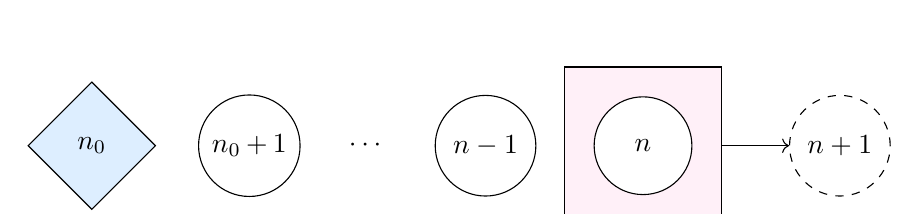
\begin{tikzpicture}
\draw[fill=indstepcol] (6,-1) rectangle (8,1);
\draw (0,0) node[diamond, draw, text width=27, text centered, fill=indbasecol] {$n_0$};
\draw (2,0) node[circle, draw, text width=27, text centered, fill=white] {$n_0+1$};
\draw (3.5,0) node {$\cdots$};
\draw (5,0) node[circle, draw, text width=27, text centered, fill=white] {$n-1$};
\draw (7,0) node[circle, draw, text width=27, text centered, fill=white] {$n$};
\draw (9.5,0) node[circle, draw, dashed, text width=27, text centered, fill=white](nplusone) {$n+1$};
\draw[->] (8,0) -- (nplusone);
\end{tikzpicture}
\end{center}

To interpret this diagram:
\begin{itemize}
\item The shaded diamond represents the base case $p(n_0)$;
\item The square represents the induction hypothesis $p(n)$;
\item The dashed circle represents the induction goal $p(n+1)$;
\item The arrow represents the implication we must prove in the induction step.
\end{itemize}

We will use analogous diagrams to illustrate the other induction principles in this section.

\begin{proposition}
\label{propSumConsecInduction}
Let $n \in \mathbb{N}$. Then $\displaystyle\sum_{k=1}^n k = \frac{n(n+1)}{2}$
\end{proposition}

\begin{cproof}
We proceed by induction on $n \ge 0$.

\begin{itemize}
\item (\textbf{Base case}) We need to prove $\displaystyle\sum_{k=1}^0 k = \frac{0(0+1)}{2}$.

This is true, since $\dfrac{0(0+1)}{2} = 0$, and $\displaystyle\sum_{k=1}^0 k = 0$ by \Cref{defSumOfRealNumbers}.

\item (\textbf{Induction step}) Let $n \ge 0$ and suppose that $\displaystyle\sum_{k=1}^n k = \dfrac{n(n+1)}{2}$; this is the induction hypothesis.

We need to prove that $\displaystyle\sum_{k=1}^{n+1} k = \frac{(n+1)(n+2)}{2}$; this is the induction goal.

We proceed by calculation:
\begin{align*}
\sum_{k=1}^{n+1} k &= \left( \sum_{k=1}^n k \right) + (n+1) && \text{by \Cref{defSumOfRealNumbers}} \\
&= \frac{n(n+1)}{2} + (n+1) && \text{by induction hypothesis}\\
&= (n+1)\left( \frac{n}{2} + 1 \right) && \text{factorising} \\
&= \frac{(n+1)(n+2)}{2} && \text{rearranging}
\end{align*}
\end{itemize}
The result follows by induction. 
\end{cproof}

Before moving on, let's reflect on the proof of \Cref{propSumConsecInduction} to highlight some effective ways of writing a proof by induction.

\begin{itemize}
\item We began the proof by indicating that it was a proof by induction. While it is clear in this section that most proofs will be by induction, that will not always be the case, so it is good practice to indicate the proof strategy at hand.
\item The base case and induction step are clearly labelled in the proof. This is not strictly \textit{necessary} from a mathematical perspective, but it helps the reader to navigate the proof and to identify what the goal is at each step.
\item We began the induction step by writing, `Let $n \ge n_0$ and suppose that [\dots{}\textit{induction hypothesis goes here}\dots{}]'. This is typically how your induction step should begin, since the proposition being proved in the induction step is of the form $\forall n \ge n_0,\, (p(n) \Rightarrow \cdots)$.
\item Before proving anything in the base case or induction step, we wrote out what it was that we were trying to prove in that part of the proof. This is helpful because it helps to remind us (and the person reading the proof) what we are aiming to achieve.
\end{itemize}

Look out for these features in the proof of the next proposition, which is also by induction on $n \ge 0$.

\begin{proposition}
The natural number $n^3-n$ is divisible by $3$ for all $n \in \mathbb{N}$.
\end{proposition}

\begin{cproof}
We proceed by induction on $n \ge 0$.
\begin{itemize}
\item (\textbf{Base case}) We need to prove that $0^3-0$ is divisible by $3$. Well
\[ 0^3-0 = 0 = 3 \times 0 \]
so $0^3-0$ is divisible by $3$.

\item (\textbf{Induction step}) Let $n \in \mathbb{N}$ and suppose that $n^3-n$ is divisible by $3$. Then $n^3-n = 3k$ for some $k \in \mathbb{Z}$.

We need to prove that $(n+1)^3 - (n+1)$ is divisible by $3$; in other words, we need to find some natural number $\ell$ such that
\[ (n+1)^3 - (n+1) = 3\ell \]
We proceed by computation.
\begin{align*}
& (n+1)^3 - (n+1) && \\
&= (n^3 + 3n^2 + 3n + 1) - n - 1 && \text{expand brackets}\\
&= n^3 - n + 3n^2 + 3n + 1 - 1 && \text{rearrange terms} \\
&= n^3 - n + 3n^2 + 3n && \text{since $1 - 1 = 0$} \\
&= 3k + 3n^2 + 3n && \text{by induction hypothesis} \\
&= 3(k+n^2+n) && \text{factorise}
\end{align*}
Thus we have expressed $(n+1)^3-(n+1)$ in the form $3\ell$ for some $\ell \in \mathbb{Z}$; specifically, $\ell=k+n^2+n$.
\end{itemize}

The result follows by induction.
\end{cproof}

\begin{exercise}
\label{exSumOfPowersOf2}
Prove by induction that $\displaystyle \sum_{k=0}^n 2^k = 2^{n+1} - 1$ for all $n \in \mathbb{N}$.
\end{exercise}

The following proposition has a proof by induction in which the base case is not zero.

\begin{proposition}
\label{propWeakInductionNonzeroBaseCaseExample}
For all $n \ge 4$, we have $3n < 2^n$.
\end{proposition}

\begin{cproof}
We proceed by induction on $n \ge 4$.
\begin{itemize}
\item (\textbf{Base case}) $p(4)$ is the statement $3 \cdot 4 < 2^4$. This is true, since $12 < 16$.

\item (\textbf{Induction step}) Suppose $n \ge 4$ and that $3n < 2^n$. We want to prove $3(n+1) < 2^{n+1}$. Well,
\begin{align*}
3(n+1) &= 3n+3 && \text{expanding} \\
&< 2^n + 3   && \text{by induction hypothesis} \\
&< 2^n + 2^4 && \text{since $3 < 16 = 2^4$} \\
&\le 2^n + 2^n && \text{since $n \ge 4$} \\
&= 2 \cdot 2^n && \text{simplifying} \\
&= 2^{n+1} && \text{simplifying}
\end{align*}
So we have proved $3(n+1) < 2^{n+1}$, as required.
\end{itemize}
The result follows by induction.
\end{cproof}

Note that the proof in \Cref{propWeakInductionNonzeroBaseCaseExample} says nothing about the truth or falsity of $p(n)$ for $n=0,1,2,3$. In order to assert that these cases are false, you need to show them individually; indeed:
\begin{itemize}
\item $3 \times 0 = 0$ and $2^0 = 1$, hence $p(0)$ is true;
\item $3 \times 1 = 3$ and $2^1 = 2$, hence $p(1)$ is false;
\item $3 \times 2 = 6$ and $2^2 = 4$, hence $p(2)$ is false;
\item $3 \times 3 = 9$ and $2^3 = 8$, hence $p(3)$ is false.
\end{itemize}
So we deduce that $p(n)$ is true when $n=0$ or $n \ge 4$, and false when $n \in \{ 1, 2, 3 \}$.

\begin{exercise}
\label{exNPowerFiveLessThanFivePowerN}
Find all natural numbers $n$ such that $n^5 < 5^n$.
\end{exercise}

\begin{exercise}
Prove that $(1+x)^{123\;456\;789} \ge 1 + 123\;456\;789\;x$ for all real $x \ge -1$.
\hintlabel{exBernoullisInequality}{%
Proving this by induction on $x$ only demonstrates that it is true for \textit{integers} $x \ge -1$, not \textit{real numbers} $x \ge -1$. Try proving a more general fact by induction on a different variable, and deducing this as a special case. (Do you \textit{really} think there is anything special about the natural number $123\;456\;789$?)}
\end{exercise}

Sometimes a `proof' by induction might appear to be complete nonsense. The following is a classic example of a `fail by induction':

\begin{example}
\label{exHorseInductionFail}
The following argument supposedly proves that every horse is the same colour.
\begin{itemize}
\item (\textbf{Base case}) Suppose there is just one horse. This horse is the same colour as itself, so the base case is immediate.
\item (\textbf{Induction step}) Suppose that every collection of $n$ horses is the same colour. Let $X$ be a set of $n+1$ horses. Removing the first horse from $X$, we see that the last $n$ horses are the same colour by the induction hypothesis. Removing the last horse from $X$, we see that the first $n$ horses are the same colour. Hence all the horses in $X$ are the same colour.
\end{itemize}
By induction, we're done.
\end{example}

\begin{exercise}
Write down the statement $p(n)$ that \Cref{exHorseInductionFail} attempted to prove for all $n \ge 1$. Convince yourself that the proof of the base case is correct, then write down---with quantifiers---exactly the proposition that the induction step is meant to prove. Explain why the argument in the induction step failed to prove this proposition.
\end{exercise}

There are several ways to avoid situations like that of \Cref{exHorseInductionFail} by simply putting more thought into writing the proof. Some tips are:

\begin{itemize}
\item State $p(n)$ explicitly. In the statement `all horses are the same colour' it is not clear exactly what the induction variable is. However, we could have said:
\begin{center}
Let $p(n)$ be the statement `every set of $n$ horses has the same colour'.
\end{center}

\item Refer explicitly to the base case $n_0$ in the induction step. In \Cref{exHorseInductionFail}, our induction hypothesis simply stated `assume every set of $n$ horses has the same colour'. Had we instead said:
\begin{center}
Let $n \ge 1$ and assume every set of $n$ horses has the same colour.
\end{center}
We may have spotted the error in what was to come.
\end{itemize}

What follows are a couple more examples of proofs by weak induction.

\begin{proposition}
For all $n \in \mathbb{N}$, we have $\displaystyle \sum_{k=0}^n k^3 = \left( \sum_{k=0}^n k \right)^2$.
\end{proposition}

\begin{cproof}
We proved in \Cref{propWeakInductionNonzeroBaseCaseExample} that $\displaystyle\sum_{k=0}^n k = \frac{n(n+1)}{2}$ for all $n \in \mathbb{N}$, thus it suffices to prove that
\[ \sum_{k=0}^n k^3 = \frac{n^2(n+1)^2}{4} \]
for all $n \in \mathbb{N}$.

We proceed by induction on $n \ge 0$.
\begin{itemize}
\item (\textbf{Base case}) We need to prove that $\displaystyle 0^3 = \frac{0^2(0+1)^2}{4}$. This is true since both sides of the equation are equal to $0$.
\item (\textbf{Induction step}) Fix $n \in \mathbb{N}$ and suppose that $\displaystyle \sum_{k=0}^n k^3 = \frac{n^2(n+1)^2}{4}$. We need to prove that $\displaystyle \sum_{k=0}^{n+1} k^3 = \frac{(n+1)^2(n+2)^2}{4}$. This is true since:
\begin{align*}
\sum_{i=0}^{n+1} k^3 & = \sum_{i=0}^n k^3 + (n+1)^3 && \text{by definition of sum} \\
&= \frac{n^2(n+1)^2}{4} + (n+1)^3 && \text{by induction hypothesis} \\
&= \frac{n^2(n+1)^2 + 4(n+1)^3}{4} && \text{(\textit{algebra})} \\
&= \frac{(n+1)^2(n^2 + 4(n+1))}{4} && \text{(\textit{algebra})} \\
&= \frac{(n+1)^2(n+2)^2}{4} && \text{(\textit{algebra})}
\end{align*}
\end{itemize}
By induction, the result follows.
\end{cproof}

In the next proposition, we prove the correctness of a well-known formula for the sum of an \textit{arithmetic progression} of real numbers.

\begin{proposition}
Let $a,d \in \mathbb{R}$. Then
\[ \sum_{k=0}^n (a+kd) = \frac{(n+1)(2a+nd)}{2} \]
for all $n \in \mathbb{N}$.
\end{proposition}

\begin{cproof}
We proceed by induction on $n \ge 0$.
\begin{itemize}
\item (\textbf{Base case}) We need to prove that $\displaystyle\sum_{k=0}^0 (a+kd) = \frac{(0+1)(2a+0d)}{2}$. This is true, since
\[ \sum_{k=0}^0 (a+kd) = a + 0d = a = \frac{2a}{2} = \frac{1 \cdot (2a)}{2} = \frac{(0+1)(2a+0d)}{2} \]

\item (\textbf{Induction step}) Fix $n \in \mathbb{N}$ and suppose that $\displaystyle\sum_{k=0}^n (a+kd) = \frac{(n+1)(2a+nd)}{2}$. We need to prove:
\[ \sum_{k=0}^{n+1} (a+kd) = \frac{(n+2)(2a+(n+1)d)}{2} \]
This is true, since
\begin{align*}
&\sum_{k=0}^{n+1} (a+kd) && \\
&= \sum_{k=0}^n (a+kd) + (a+(n+1)d) && \text{by definition of sum} \\
&= \frac{(n+1)(2a+nd)}{2} + (a + (n+1)d) && \text{by induction hypothesis} \\
&= \frac{(n+1)(2a+nd) + 2a + 2(n+1)d}{2} && \text{(\textit{algebra})} \\
&= \frac{(n+1) \cdot 2a + (n+1) \cdot nd + 2a + 2(n+1)d}{2} && \text{(\textit{algebra})} \\
&= \frac{2a(n+1+1) + (n+1)(nd + 2d)}{2} && \text{(\textit{algebra})} \\
&= \frac{2a(n+2) + (n+1)(n+2)d}{2} && \text{(\textit{algebra})} \\
&= \frac{(n+2)(2a + (n+1)d)}{2} && \text{(\textit{algebra})}
\end{align*}
\end{itemize}
By induction, the result follows.
\end{cproof}

The following exercises generalises \Cref{exSumOfPowersOf2} to prove the correctness of a formula for the sum of a \textit{geometric progression} of real numbers.

\begin{exercise}
\label{exFormulaForGeometricProgression}
Let $a,r \in \mathbb{R}$ with $r \ne 1$. Then
\[ \sum_{k=0}^n ar^k = \frac{a(1-r^{n+1})}{1-r} \]
for all $n \in \mathbb{N}$. [You may assume that $r^ir^j=r^{i+j}$ for all $i,j \in \mathbb{N}$.]
\end{exercise}

When attempting the following exercise, you might find that your induction step requires an auxiliary result, which itself has a proof by induction.

\begin{exercise}
Prove by induction that $7^n - 2 \cdot 4^n + 1$ is divisible by $18$ for all $n \in \mathbb{N}$.
\hintlabel{exInductionEmbeddedInIductionStep}{%
Observe that $7^{n+1} - 2 \cdot 4^{n+1} + 1 = 4(7^n - 2 \cdot 4^n + 1) + 3(7^n - 1)$ for all $n \in \mathbb{N}$.
}
\end{exercise}

So far in this section most of the results that we have proved by induction have concerned numbers, and particularly identities involving natural numbers. But the scope of proof by induction is not limited to such results---the next exercise, for example, concerns sets and bijections.

\begin{exercise}
Let $n \in \mathbb{N}$ and let $\{ X_k \mid 1 \le k \le n \}$ be a family of sets. Prove by induction on $n$ that there is a bijection $\displaystyle \prod_{k=1}^{n+1} X_k \to \left( \prod_{k=1}^n X_k \right) \times X_n$.
\hintlabel{exProductOfSuccNSets}{%
To define the bijection, think about what the elements of the two sets look like: The elements of $\prod_{k=1}^{n+1} X_k$ look like $(a_1, a_2, \dots, a_n, a_{n+1})$, where $a_k \in X_k$ for each $1 \le k \le n+1$. On the other hand, the elements of $\left( \prod_{k=1}^n X_k \right) \times X_{n+1}$ look like $((a_1, a_2, \dots, a_n), a_{n+1})$.
}
\end{exercise}

\subsection*{Binomials and factorials}

Proof by induction turns out to be a very useful way of proving facts about binomial coefficients $\binom{n}{k}$ and factorials $n!$.

\begin{example}
\label{exSumOfBinomialCoefficients}
We prove that $\sum_{i=0}^n \binom{n}{i} = 2^n$ by induction on $n$.
\begin{itemize}
\item (\textbf{Base case}) We need to prove $\binom{0}{0} = 1$ and $2^0=1$. These are both true by the definitions of binomial coefficients and exponents.
\item (\textbf{Induction step}) Fix $n \ge 0$ and suppose that
\[ \sum_{i=0}^n \binom{n}{i} = 2^n \]
We need to prove
\[ \sum_{i=0}^{n+1} \binom{n+1}{i} = 2^{n+1} \]
This is true, since

\begin{align*}
&\sum_{i=0}^{n+1} \binom{n+1}{i} && \\
&= \binom{n+1}{0} + \sum_{i=1}^{n+1} \binom{n+1}{i} && \text{splitting the sum} \\
&= 1 + \sum_{j=0}^n \binom{n+1}{j+1} && \text{letting $j=i-1$} \\
&= 1 + \sum_{j=0}^n \left(\binom{n}{j} + \binom{n}{j+1}\right) && \text{by \Cref{defBinomialCoefficientRecursive}} \\
&= 1 + \sum_{j=0}^n \binom{n}{j} + \sum_{j=0}^n \binom{n}{j+1} && \text{separating the sums}
\end{align*}

Now $\sum_{j=0}^n \binom{n}{j} = 2^n$ by the induction hypothesis. Moreover, reindexing the sum using $k=j+1$ yields
\[ \sum_{j=0}^n \binom{n}{j+1} = \sum_{k=1}^{n+1} \binom{n}{k} = \sum_{k=1}^n \binom{n}{k} + \binom{n}{n+1} \]
By the induction hypothesis, we have
\[ \sum_{k=1}^n \binom{n}{k} = \sum_{k=0}^n \binom{n}{k} - \binom{n}{0} = 2^n-1 \]
and $\binom{n}{n+1} = 0$, so that $\sum_{j=0}^n \binom{n}{j+1} = 2^n-1$.

Putting this together, we have
\begin{align*}
1 + \sum_{j=0}^n \binom{n}{j} + \sum_{j=0}^n \binom{n}{j+1}
&= 1 + 2^n + (2^n-1) \\
&= 2 \cdot 2^n \\
&= 2^{n+1}
\end{align*}
so the induction step is finished.
\end{itemize}
By induction, we're done.
\end{example}

\begin{exercise}
\label{exAlternatingSumOfBinomialCoefficientsIsZero}
Prove by induction on $n \ge 1$ that
\[ \sum_{i=0}^n (-1)^i \binom{n}{i} = 0 \]
\end{exercise}

\begin{theorem}
\label{thmBinomAsFactorialByInduction}
Let $n,k \in \mathbb{N}$. Then
\[ \binom{n}{k} =
\begin{cases}
\dfrac{n!}{k!(n-k)!} & \text{if } k \le n \\
0 & \text{if } k > n
\end{cases} \]
\end{theorem}
\begin{cproof}
We proceed by induction on $n$.
\begin{itemize}
\item (\textbf{Base case}) When $n=0$, we need to prove that $\binom{0}{k} = \frac{0!}{k!(-k)!}$ for all $k \le 0$, and that $\binom{0}{k} = 0$ for all $k>0$.

If $k \le 0$ then $k=0$, since $k \in \mathbb{N}$. Hence we need to prove
\[ \binom{0}{0} = \frac{0!}{0!0!} \]
But this is true since $\binom{0}{0}=1$ and $\frac{0!}{0!0!} = \frac{1}{1 \times 1} = 1$.

If $k>0$ then $\binom{0}{k} = 0$ by \Cref{defBinomialCoefficientRecursive}.
\item (\textbf{Induction step}) Fix $n \in \mathbb{N}$ and suppose that $\binom{n}{k} = \frac{n!}{k!(n-k)!}$ for all $k \le n$ and $\binom{n}{k} = 0$ for all $k > n$.

We need to prove that, for all $k \le n+1$, we have
\[ \binom{n+1}{k} = \frac{(n+1)!}{k!(n+1-k)!} \]
and that $\binom{n+1}{k} = 0$ for all $k > n+1$.

So fix $k \in \mathbb{N}$. There are four possible cases: either (i) $k=0$, or (ii) $0 < k \le n$, or (iii) $k=n+1$, or (iv) $k>n+1$. In cases (i), (ii) and (iii), we need to prove the factorial formula for $\binom{n+1}{k}$; in case (iv), we need to prove that $\binom{n+1}{k} = 0$.

\begin{enumerate}[(i)]
\item Suppose $k=0$. Then $\binom{n+1}{0} = 1$ by \Cref{defBinomialCoefficientRecursive}, and
\[ \frac{(n+1)!}{k!(n+1-k)!} = \frac{(n+1)!}{0!(n+1)!} = 1 \]
since $0!=1$. So $\binom{n+1}{0} = \frac{(n+1)!}{0!(n+1)!}$.
\item If $0 < k \le n$ then $k=\ell+1$ for some natural number $\ell < n$. Then $\ell+1 \le n$, so we can use the induction hypothesis to apply factorial formula to both $\binom{n}{\ell}$ and $\binom{n}{\ell+1}$. Hence
\begin{align*}
&\binom{n+1}{k} && \\
&= \binom{n+1}{\ell+1} && \text{since $k=\ell+1$} \\
&= \binom{n}{\ell} + \binom{n}{\ell+1} && \text{by \Cref{defBinomialCoefficientRecursive}} \\
&= \frac{n!}{\ell!(n-\ell)!} + \frac{n!}{(\ell+1)!(n-\ell-1)!} && \text{by induction hypothesis}
\end{align*}
Now note that
\[ \frac{n!}{\ell!(n-\ell)!} = \frac{n!}{\ell!(n-\ell)!} \cdot \frac{\ell+1}{\ell+1} = \frac{n!}{(\ell+1)!(n-\ell)!} \cdot (\ell+1) \]
and
\begin{center}
$\dfrac{n!}{(\ell+1)!(n-\ell-1)!} = \dfrac{n!}{(\ell+1)!(n-\ell-1)!} \cdot \dfrac{n-\ell}{n-\ell} = \dfrac{n!}{(\ell+1)!(n-\ell)!} \cdot (n-\ell)$
\end{center}

Piecing this together, we have
\begin{align*}
&\frac{n!}{\ell!(n-\ell)!} + \frac{n!}{(\ell+1)!(n-\ell-1)!} && \\
&= \frac{n!}{(\ell+1)!(n-\ell)!} \cdot [(\ell+1) + (n-\ell)] \\
&= \frac{n!(n+1)}{(\ell+1)!(n-\ell)!} && \\
&= \frac{(n+1)!}{(\ell+1)!(n-\ell)!}
\end{align*}
so that $\binom{n+1}{\ell+1} = \frac{(n+1)!}{(\ell+1)!(n-\ell)!}$. Now we're done; indeed,
\[ \frac{(n+1)!}{(\ell+1)!(n-\ell)!} = \frac{(n+1)!}{k!(n+1-k)!} \]
since $k=\ell+1$.
\item If $k=n+1$, then
\begin{align*}
\binom{n+1}{k} &= \binom{n+1}{n+1} && \text{since $k=n+1$} \\
&= \binom{n}{n} + \binom{n}{n+1} && \text{by \Cref{defBinomialCoefficientRecursive}} \\
&= \frac{n!}{n!0!} + 0 && \text{by induction hypothesis} \\
&= 1
\end{align*}
and $\frac{(n+1)!}{(n+1)!0!}=1$, so again the two quantities are equal.
\item If $k>n+1$, then $k=\ell+1$ for some $\ell > n$, and so by \Cref{defBinomialCoefficientRecursive} and the induction hypothesis we have
\[ \binom{n+1}{k} = \binom{n+1}{\ell+1} \overset{\text{IH}}{=} \binom{n}{\ell}+\binom{n}{\ell+1} = 0+0 = 0 \]

\end{enumerate}
\end{itemize}
\end{cproof}

On first reading, this proof is long and confusing, especially in the induction step where we are required to split into four cases. We will give a much simpler proof in \Cref{secCountingPrinciples} (see \Cref{thmBinomAsFactorial}), where we prove the statement \textit{combinatorially} by putting the elements of two sets in one-to-one correspondence.

We can use \Cref{thmBinomAsFactorialByInduction} to prove useful identities involving binomial coefficients.

\begin{example}
Let $n,k,\ell \in \mathbb{N}$ with $\ell \le k \le n$ then \[ \binom{n}{k}\binom{k}{\ell} = \binom{n}{\ell}\binom{n-\ell}{k-\ell} \]
Indeed:
\begin{align*}
& \binom{n}{k} \binom{k}{\ell} && \\
&= \frac{n!}{k!(n-k)!} \cdot \frac{k!}{\ell!(k-\ell!)} && \text{by \Cref{thmBinomAsFactorialByInduction}} \\
&= \frac{n!k!}{k!\ell!(n-k)!(k-\ell)!} && \text{combine fractions} \\
&= \frac{n!}{\ell!(n-k)!(k-\ell)!} && \text{cancel } k!\\
&= \frac{n!(n-\ell)!}{\ell!(n-k)!(k-\ell)!(n-\ell)!} && \text{multiply by } \frac{(n-\ell)!}{(n-\ell)!} \\
&= \frac{n!}{\ell!(n-\ell!)} \cdot \frac{(n-\ell)!}{(k-\ell)!(n-k)!} && \text{separate fractions} \\
&= \frac{n!}{\ell!(n-\ell!)} \cdot \frac{(n-\ell)!}{(k-\ell)!((n-\ell)-(k-\ell))!} && \text{rearranging} \\
&= \binom{n}{\ell} \binom{n-\ell}{k-\ell} && \text{by \Cref{thmBinomAsFactorialByInduction}}
\end{align*}
\end{example}

\begin{exercise}
Prove that $\binom{n}{k} = \binom{n}{n-k}$ for all $n,k \in \mathbb{N}$ with $k \le n$.
\end{exercise}

A very useful application of binomial coefficients in elementary algebra is to the binomial theorem.

\begin{theorem}[Binomial theorem]
\label{thmBinomialTheorem}
Let $n \in \mathbb{N}$ and $x,y \in \mathbb{R}$. Then
\[ (x+y)^n = \sum_{k=0}^n \binom{n}{k} x^k y^{n-k} \]
\end{theorem}
\begin{cproof}
In the case when $y=0$ we have $y^{n-k}=0$ for all $k<n$, and so the equation reduces to
\[ x^n = x^ny^{n-n} \]
which is true, since $y^0=1$. So for the rest of the proof, we will assume that $y \ne 0$.

We will now reduce to the case when $y=1$; and extend to arbitrary $y \ne 0$ afterwards.

We prove $(1+x)^n = \sum_{k=0}^n \binom{n}{k} x^k$ by induction on $n$.
\begin{itemize}
\item (\textbf{Base case}) $(1+x)^0=1$ and $\binom{0}{0} x^0 = 1 \cdot 1 = 1$, so the statement is true when $n=0$.
\item (\textbf{Induction step}) Fix $n \in \mathbb{N}$ and suppose that
\[ (1+x)^n = \sum_{k=0}^n \binom{n}{k} x^k \]

We need to show that $(1+x)^{n+1} = \sum_{k=0}^{n+1} \binom{n+1}{k} x^k$. Well,

\begin{align*} \hspace{-30pt}
& (1+x)^{n+1} && \\
&= (1+x)(1+x)^n && \text{by laws of indices} \\
&= (1+x) \cdot \sum_{k=0}^n \binom{n}{k} x^k && \text{by induction hypothesis} \\
&= \sum_{k=0}^n \binom{n}{k} x^k + x \cdot \sum_{k=0}^n \binom{n}{k} x^{k}&& \text{by expanding $(x+1)$} \\
&= \sum_{k=0}^n \binom{n}{k} x^k + \sum_{k=0}^n \binom{n}{k} x^{k+1} && \text{distributing $x$} \\
&= \sum_{k=0}^n \binom{n}{k} x^k + \sum_{k=1}^{n+1} \binom{n}{k-1} x^k && \text{$k \to k-1$ in second sum} \\
&= \binom{n}{0}x^0 + \sum_{k=1}^n \left( \binom{n}{k} + \binom{n}{k-1} \right) x^k + \binom{n}{n}x^{n+1} && \text{splitting the sums} \\
&= \binom{n}{0}x^0 + \sum_{k=1}^n \binom{n+1}{k} x^k + \binom{n}{n}x^{n+1} && \text{by \Cref{defBinomialCoefficientRecursive}} \\
&= \binom{n+1}{0}x^0 + \sum_{k=1}^n \binom{n+1}{k} x^k + \binom{n+1}{n+1}x^{n+1} && \text{see $(*)$ below} \\
&= \sum_{k=0}^{n+1} \binom{n+1}{k} x^k &&
\end{align*}
The step labelled $(*)$ holds because
\[ \binom{n}{0} = 1 = \binom{n+1}{0} \qquad \text{and} \qquad \binom{n}{n} = 1 = \binom{n+1}{n+1} \]
\end{itemize}
By induction, we've shown that $(1+x)^n = \sum_{i=0}^n \binom{n}{k} x^k$ for all $n \in \mathbb{N}$.

When $y \ne 0$ is not necessarily equal to $1$, we have that
\[ (x+y)^n = y^n \cdot \left( 1 + \frac{x}{y} \right)^n = y^n \cdot \sum_{k=0}^n \binom{n}{k} \left( \frac{x}{y} \right)^k = \sum_{k=0}^n \binom{n}{k} x^k y^{n-k} \]
The middle equation follows by what we just proved; the leftmost and rightmost equations are simple algebraic rearrangements.
\end{cproof}

\begin{example}
In \Cref{exSumOfBinomialCoefficients} we saw that
\[ \sum_{k=0}^n \binom{n}{k} = 2^n \]
This follows quickly from the binomial theorem, since
\[ 2^n = (1+1)^n = \sum_{k=0}^n \binom{n}{k} \cdot 1^k \cdot 1^{n-k} = \sum_{k=0}^n \binom{n}{k} \]
Likewise, in \Cref{exAlternatingSumOfBinomialCoefficientsIsZero} you proved that the alternating sum of binomial coefficients is zero; that is, for $n \in \mathbb{N}$, we have
\[ \sum_{k=0}^n (-1)^k \binom{n}{k} = 0 \]
The proof is greatly simplified by applying the binomial theorem. Indeed, by the binomial theorem, we have
\[ 0 = 0^n = (-1+1)^n = \sum_{k=0}^n \binom{n}{k}(-1)^k1^{n-k} = \sum_{k=0}^n (-1)^k \binom{n}{k} \]
Both of these identities can be proved much more elegantly, quickly and easily using \textit{enumerative combinatorics}. This will be the topic covered in \Cref{secCountingPrinciples}.
\end{example}

\index{induction!weak|)}

\newpage
% !TeX root = ../../book.tex
\section{Strong induction}
\secbegin{secStrongInduction}
\index{induction!strong|(}

Consider the following example, which we will attempt to prove by induction.

\begin{example}
\label{exProofByWeakInductionFail}
Define a sequence recursively by
\[ b_0 = 1 \quad \text{and} \quad b_{n+1} = 1 + \sum_{k=0}^n b_k \text{ for all } n \in \mathbb{N} \]
We will attempt to prove by induction that $b_n = 2^n$ for all $n \in \mathbb{N}$.

\begin{itemize}
\item (\textbf{Base case}) By definition of the sequence we have $b_0=1=2^0$. So far so good.

\item (\textbf{Induction step}) Fix $n \in \mathbb{N}$, and suppose that $b_n = 2^n$. We need to show that $b_{n+1}=2^{n+1}$.

Well, $b_{n+1} = 1 + \sum_{k=0}^n b_k = {\dots}$ uh oh.
\end{itemize}

Here's what went wrong. If we could replace each $b_k$ by $2^k$ in the sum, then we'd be able to complete the proof. However we cannot justify this substitution: our induction hypothesis only gives us information about $b_n$, not about a general term $b_k$ for $k < n$.
\end{example}

The \textit{strong} induction principle looks much like the weak induction principle, except that its induction hypothesis is more powerful. Despite its name, strong induction is no stronger than weak induction; the two principles are equivalent. In fact, we'll prove the strong induction principle \textit{by weak induction}!

\begin{theorem}[Strong induction principle]
\label{thmStrongInduction}
\index{induction!on $\mathbb{N}$ (strong)}
\index{strong induction principle}
Let $p(n)$ be a logical formula with free variable $n \in \mathbb{N}$ and let $n_0 \in \mathbb{N}$. If
\begin{enumerate}[(i)]
\item $p(n_0)$ is true; and
\item For all $n \ge n_0$, if $p(k)$ is true for all $n_0 \le k \le n$, then $p(n+1)$ is true;
\end{enumerate}
then $p(n)$ is true for all $n \ge n_0$.
\end{theorem}

\begin{cproof}
For each $n \ge n_0$, let $q(n)$ be the assertion that $p(k)$ is true for all $n_0 \le k \le n$.

%% BEGIN EXTRACT (xtrAssumingImplicationsExample) %%
Notice that $q(n)$ implies $p(n)$ for all $n \ge n_0$, since given $n \ge n_0$, if $p(k)$ is true for all $n_0 \le k \le n$, then in particular $p(k)$ is true when $k=n$.

So it suffices to prove $q(n)$ is true for all $n \ge n_0$.
%% END EXTRACT %%
We do so by weak induction.

\begin{itemize}
\item (\textbf{Base case}) $q(n_0)$ is equivalent to $p(n_0)$, since the only natural number $k$ with $n_0 \le k \le n_0$ is $n_0$ itself; hence $q(n_0)$ is true by condition (i).

\item (\textbf{Induction step}) Let $n \ge n_0$ and suppose $q(n)$ is true. Then $p(k)$ is true for all $n_0 \le k \le n$.

We need to prove that $q(n+1)$ is true---that is, that $p(k)$ is true for all $n_0 \le k \le n+1$. But we know $p(k)$ is true for all $n_0 \le k \le n$---this is the induction hypothesis---and then $p(n+1)$ is true by condition (ii). So we have that $p(k)$ is true for all $n_0 \le k \le n+1$ after all.
\end{itemize}
By induction, $q(n)$ is true for all $n \ge n_0$. Hence $p(n)$ is true for all $n \ge n_0$.
\end{cproof}

\begin{strategy}[Proof by strong induction]
\label{strStrongInduction}
\index{proof!by strong induction}
In order to prove a proposition of the form $\forall n \ge n_0,\, p(n)$, it suffices to prove that $p(n_0)$ is true and that, for all $n \ge n_0$, if $p(k)$ is true for all $n_0 \le k \le n$, then $p(n+1)$ is true.
\end{strategy}

Like with weak induction, we can illustrate how strong induction works diagrammatically. The induction hypothesis, represented by the large square, now encompasses $p(k)$ for all $n_0 \le k \le n$, where $p(n_0)$ is the base case.

\begin{center}
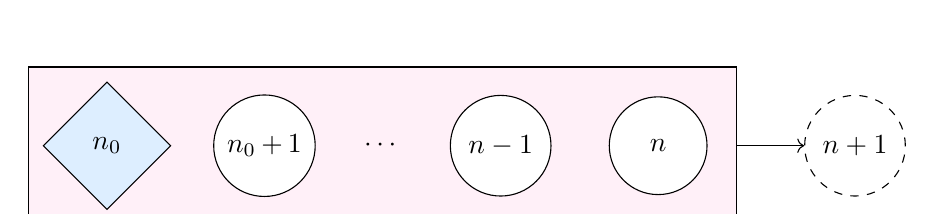
\begin{tikzpicture}
\draw[fill=indstepcol] (-1,-1) rectangle (8,1);
\draw (0,0) node[diamond, draw, text width=27, text centered, fill=indbasecol] {$n_0$};
\draw (2,0) node[circle, draw, text width=27, text centered, fill=white] {$n_0+1$};
\draw (3.5,0) node {$\cdots$};
\draw (5,0) node[circle, draw, text width=27, text centered, fill=white] {$n-1$};
\draw (7,0) node[circle, draw, text width=27, text centered, fill=white] {$n$};
\draw (9.5,0) node[circle, draw, dashed, text width=27, text centered, fill=white](nplusone) {$n+1$};
\draw[->] (8,0) -- (nplusone);
\end{tikzpicture}
\end{center}

Observe that the only difference from weak induction is the induction hypothesis.
\begin{itemize}
\item \textbf{Weak induction step:} Fix $n \ge n_0$, \fbox{assume $p(n)$ is true}~, derive $p(n+1)$;
\item \textbf{Strong induction step:} Fix $n \ge n_0$, \fbox{assume $p(k)$ is true for all $n_0 \le k \le n$}~, derive $p(n+1)$.
\end{itemize}

We now use strong induction to complete the proof of \Cref{exProofByWeakInductionFail}.

\begin{example}[\Cref{exProofByWeakInductionFail} revisited]
Define a sequence recursively by
\[ b_0 = 1 \quad \text{and} \quad b_{n+1} = 1 + \sum_{k=0}^n b_k \text{ for all } n \in \mathbb{N} \]
We will prove by strong induction that $b_n = 2^n$ for all $n \in \mathbb{N}$.

\begin{itemize}
\item (\textbf{Base case}) By definition of the sequence we have $b_0=1=2^0$.
\item (\textbf{Induction step}) Fix $n \in \mathbb{N}$, and suppose that $b_k=2^k$ for all $k \le n$. We need to show that $b_{n+1}=2^{n+1}$. This is true, since
\begin{align*}
b_{n+1} &= 1 + \sum_{k=0}^n b_k && \text{by the recursive formula for $b_{n+1}$} \\
&= 1 + \sum_{k=0}^n 2^k && \text{by the induction hypothesis} \\
&= 1 + (2^{n+1}-1) && \text{by \Cref{exSumOfPowersOf2}} \\
&= 2^{n+1}
\end{align*}
\end{itemize}
By induction, it follows that $b_n=2^n$ for all $n \in \mathbb{N}$.
\end{example}

The following theorem adapts the strong induction principle to proofs where we need to refer to a \textit{fixed} number of previous steps in our induction step.

\begin{theorem}[Strong induction principle {(multiple base cases)}]
\label{thmSIPMultipleBaseCases}
Let $p(n)$ be a logical formula with free variable $n \in \mathbb{N}$ and let $n_0 < n_1 \in \mathbb{N}$. If
\begin{enumerate}[(i)] \vspace{5pt} 
\item $p(n_0), p(n_0+1), \dots, p(n_1)$ are all true; and
\item For all $n \ge n_1$, if $p(k)$ is true for all $n_0 \le k \le n$, then $p(n+1)$ is true;
\end{enumerate}
\vspace{5pt}
then $p(n)$ is true for all $n \ge n_0$.
\end{theorem}

\begin{cproof}
The fact that $p(n)$ is true for all $n \ge n_0$ follows from strong induction. Indeed:
\begin{itemize}
\item (\textbf{Base case}) $p(n_0)$ is true by (i);
\item (\textbf{Induction step}) Fix $n \ge n_0$ and assume $p(k)$ is true for all $n_0 \le k \le n$. Then:
\begin{itemize}
\item If $n < n_1$, then $n+1 \le n_1$, so that $p(n)$ is true by (i);
\item If $n \ge n_1$, then $p(n+1)$ is true by (ii).
\end{itemize}
In both cases we see that $p(n+1)$ is true, as required.
\end{itemize}
Thus by strong induction, we have that $p(n)$ is true for all $n \ge n_0$.
\end{cproof}

\begin{strategy}[Proof by strong induction with multiple base cases]
\index{proof!by strong induction with multiple base cases}
In order to prove a statement of the form $\forall n \ge n_0,\, p(n)$, it suffices to prove $p(k)$ for all $k \in \{ n_0, n_0+1, \dots, n_1 \}$, where $n_1 > n_0$, and then given $n \ge n_1$, assuming $p(k)$ is true for all $n_0 \le k \le n$, prove that $p(n+1)$ is true.
\end{strategy}

This kind of strong induction differs from the usual kind in two main ways:
\begin{itemize}
\item There are multiple base cases $p(n_0), p(n_0+1), \dots, p(n_1)$, not just one.
\item The induction step refers to both the least base case $n_0$ and the greatest base case $n_1$: the variable $n$ in the induction step is taken to be greater than or equal to $n_1$, while the induction hypothesis assumes $p(k)$ for all $n_0 \le k \le n$.
\end{itemize}

The following diagram illustrates how strong induction with multiple base cases works.

\begin{center}
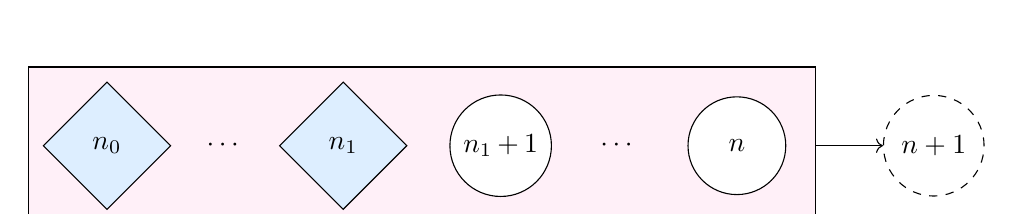
\begin{tikzpicture}
\draw[fill=indstepcol] (-1,-1) rectangle (9,1);
\draw (0,0) node[diamond, draw, text width=27, text centered, fill=indbasecol] {$n_0$};
\draw (1.5,0) node {$\cdots$};
\draw (3,0) node[diamond, draw, text width=27, text centered, fill=indbasecol] {$n_1$};
\draw (5,0) node[circle, draw, text width=27, text centered, fill=white] {$n_1+1$};
\draw (6.5,0) node {$\cdots$};
\draw (8,0) node[circle, draw, text width=27, text centered, fill=white] {$n$};
\draw (10.5,0) node[circle, draw, dashed, text width=27, text centered, fill=white](nplusone) {$n+1$};
\draw[->] (9,0) -- (nplusone);
\end{tikzpicture}
\end{center}

Note the difference in quantification of variables in the induction step between regular strong induction and strong induction with multiple base cases:
\begin{itemize}
\item \textbf{One base case.} Fix $n \ge \boxed{n_0}$ and assume $p(k)$ is true for all $\boxed{n_0} \le k \le n$.
\item \textbf{Multiple base cases.} Fix $n \ge \boxed{n_1}$ and assume $p(k)$ is true for all $\boxed{n_0} \le k \le n$.
\end{itemize}

Getting the quantification of the variables $n$ and $k$ in the strong induction step is crucial, since the quantification affects what may be assumed about $n$ and $k$.

The need for multiple base cases often arises when proving results about recursively defined sequences, where the definition of a general term depends on the values of a fixed number of previous terms.

\begin{example}
Define the sequence
\[ a_0 = 0, \quad a_1 = 1, \quad a_n = 3a_{n-1} - 2a_{n-2} \text{ for all } n \ge 2 \]
We find and prove a general formula for $a_n$ in terms of $n$. Writing out the first few terms in the sequence establishes a pattern that we might attempt to prove:
\begin{center}
\begin{tabular}{c|ccccccccc}
$n$   & $0$ & $1$ & $2$ & $3$ & $4$  & $5$  & $6$  & $7$   & $8$ \\ \hline
$a_n$ & $0$ & $1$ & $3$ & $7$ & $15$ & $31$ & $63$ & $127$ & $255$
\end{tabular}
\end{center}

It appears that $a_n = 2^n - 1$ for all $n \ge 0$. We prove this by strong induction, taking the cases $n=0$ and $n=1$ as our base cases.

\begin{itemize}
\item (\textbf{Base cases}) By definition of the sequence, we have:
\begin{itemize}
\item $a_0 = 0 = 2^0 - 1$; and
\item $a_1 = 1 = 2^1 - 1$;
\end{itemize}
so the claim is true when $n=0$ and $n=1$.

\item (\textbf{Induction step}) Fix $n \ge 1$ and assume that $a_k = 2^k - 1$ for all $0 \le k \le n$. We need to prove that $a_{n+1} = 2^{n+1} - 1$.

Well since $n \ge 1$, we have $n+1 \ge 2$, so we can apply the recursive formula to $a_{n+1}$. Thus
\begin{align*}
a_{n+1} &= 3a_n - 2a_{n-1} && \text{by definition of $a_{n+1}$} \\
&= 3(2^n-1) - 2(2^{n-1}-1) && \text{by induction hypothesis} \\
&= 3 \cdot 2^n - 3 - 2 \cdot 2^{n-1} + 2 && \text{expanding} \\
&= 3 \cdot 2^n - 3 - 2^n + 2 && \text{using laws of indices} \\
&= 2 \cdot 2^n - 1 && \text{simplifying} \\
&= 2^{n+1} - 1 && \text{using laws of indices}
\end{align*}
\end{itemize}
So the result follows by induction.
\end{example}

The following exercises have proofs by strong induction with multiple base cases.

\begin{exercise}
Define a sequence recursively by $a_0 = 4$, $a_1 = 9$ and $a_n = 5a_{n-1} - 6a_{n-2}$ for all $n \ge 2$. Prove that $a_n = 3 \cdot 2^n + 3^n$ for all $n \in \mathbb{N}$.
\end{exercise}

\begin{exercise}
The \textit{Tribonacci sequence} is the sequence $t_0, t_1, t_2, \dots$ defined by
\[ t_0 = 0, \quad t_1 = 0, \quad t_2 = 1, \quad t_n = t_{n-1} + t_{n-2} + t_{n-3} \text{ for all } n \ge 3 \]
Prove that $t_n \le 2^{n-3}$ for all $n \ge 3$.
\end{exercise}

\begin{exercise}
The \textit{Frobenius coin problem} asks when a given amount of money can be obtained from coins of given denominations. For example, a value of $7$ dubloons cannot be obtained using only $3$ dubloon and $5$ dubloon coins, but for all $n \ge 8$, a value of $n$ dubloons \textit{can} be obtained using only $3$ dubloon and $5$ dubloon coins. Prove this.
\hintlabel{exFrobeniusCoinProblem}{%
Observe that if $n$ dubloons can be obtained using only $3$ and $5$ dubloon coins, then so can $n+3$. See how you might use this fact to exploit strong induction with multiple base cases.
}
\end{exercise}

\subsection*{Well-ordering principle}

The underlying reason why we can perform induction and recursion on the natural numbers is because of the way they are ordered. Specifically, the natural numbers satisfy the \textit{well-ordering principle}: if a set of natural numbers has at least one element, then it has a least element. This sets the natural numbers apart from the other number sets; for example, $\mathbb{Z}$ has no least element, since if $a \in \mathbb{Z}$ then $a-1 \in \mathbb{Z}$ and $a-1 < a$.

\begin{theorem}[Well-ordering principle]
\label{thmWellOrderingPrinciple}
\index{well-ordering principle}
Let $X$ be a set of natural numbers. If $X$ is inhabited, then $X$ has a least element.
\end{theorem}

\begin{cidea}
Under the assumption that $X$ is a set of natural numbers, the proposition we want to prove has the form $p \Rightarrow q$. Namely
\[ X \text{ is inhabited} \quad \Rightarrow \quad X \text{ has a least element} \]
Assuming $X$ is inhabited doesn't really give us much to work with, so let's try the contrapositive:
\[ X \text{ has no least element} \quad \Rightarrow \quad X \text{ is empty} \]
The assumption that $X$ has no least element \textit{does} give us something to work with. Under this assumption we need to deduce that $X$ is empty.

We will do this by `forcing $X$ up' by strong induction. Certainly $0 \not \in X$, otherwise it would be the least element. If none of the numbers $0, 1, \dots, n$ are elements of $X$ then neither can $n+1$ be, since if it were then \textit{it} would be the least element of $X$. Let's make this argument formal.
\end{cidea}

\begin{cproof}
Let $X$ be a set of natural numbers containing no least element. We prove by strong induction that $n \not \in X$ for all $n \in \mathbb{N}$.

\begin{itemize}
\item (\textbf{Base case}) $0 \not \in X$ since if $0 \in X$ then $0$ must be the least element of $X$, as it is the least natural number.
\item (\textbf{Induction step}) Suppose $k \not \in X$ for all $0 \le k \le n$. If $n+1 \in X$ then $n+1$ is the least element of $X$; indeed, if $\ell < n+1$ then $0 \le \ell \le n$, so $\ell \not \in X$ by the induction hypothesis. This contradicts the assumption that $X$ has no least element, so $n+1 \not \in X$.
\end{itemize}
By strong induction, $n \not \in X$ for each $n \in \mathbb{N}$. Since $X$ is a set of natural numbers, and it contains no natural numbers, it follows that $X$ is empty.
\end{cproof}

The following proof that $\sqrt{2}$ is irrational is a classic application of the well-ordering principle.

\begin{proposition}
\label{propSqrt2Irrational}
The number $\sqrt{2}$ is irrational.
\end{proposition}

To prove \Cref{propSqrt2Irrational} we will use the following lemma, which uses the well-ordering principle to prove that fractions can be `cancelled to lowest terms'.

\begin{lemma}
\label{lemFractionInLowestTerms}
Let $q$ be a positive rational number. There is a pair of nonzero natural numbers $a,b$ such that $q=\frac{a}{b}$ and such that the only natural number which divides both $a$ and $b$ is $1$.
\end{lemma}

\begin{cproof}
First note that we can express $q$ as the ratio of two nonzero natural numbers, since $q$ is a positive rational number. By the well-ordering principle, there is a \textit{least} natural number $a$ such that $q=\frac{a}{b}$ for some positive $b \in \mathbb{N}$.

Suppose that some natural number $d$ other than $1$ divides both $a$ and $b$. Note that $d \ne 0$, since if $d=0$ then that would imply $a=0$. Since $d \ne 1$, it follows that $d \ge 2$.

Since $d$ divides $a$ and $b$, there exist natural numbers $a',b'$ such that $a=a'd$ and $b=b'd$. Moreover, $a',b'>0$ since $a,b,d > 0$. It follows that
\[ q = \frac{a}{b} = \frac{a'd}{b'd} = \frac{a'}{b'} \]
But $d \ge 2$, and hence
\[ a' = \frac{a}{d} \le \frac{a}{2} < a \]
contradicting minimality of $a$. Hence our assumption that some natural number $d$ other than $1$ divides both $a$ and $b$ was false---it follows that the only natural number dividing both $a$ and $b$ is $1$.
\end{cproof}

We are now ready to prove that $\sqrt{2}$ is irrational.

\begin{cproof}[of \Cref{propSqrt2Irrational}]
Suppose $\sqrt{2}$ is rational. Since $\sqrt{2}>0$, this means that we can write
\[ \sqrt{2} = \frac{a}{b} \]
where $a$ and $b$ are both positive natural numbers. By \Cref{lemFractionInLowestTerms}, we may assume that the only natural number dividing $a$ and $b$ is $1$.

Multiplying the equation $\sqrt{2} = \frac{a}{b}$ and squaring yields
\[ a^2=2b^2 \]
Hence $a^2$ is even. By \Cref{propIfProductEvenThenSomeFactorEven}, $a$ is even, so we can write $a=2c$ for some $c > 0$. Then $a^2=(2c)^2=4c^2$, and hence
\[ 4c^2=2b^2 \]
Dividing by $2$ yields
\[ 2c^2 = b^2 \]
and hence $b^2$ is even. By \Cref{propIfProductEvenThenSomeFactorEven} again, $b$ is even.

But if $a$ and $b$ are both even, the natural number $2$ divides both $a$ and $b$. This contradicts the fact that the only natural number dividing both $a$ and $b$ is $1$. Hence our assumption that $\sqrt{2}$ is rational is incorrect, and $\sqrt{2}$ is irrational.
\end{cproof}

\begin{writingtip}
In the proof of \Cref{propSqrt2Irrational} we could have separately proved that $a^2$ being even implies $a$ is even, and that $b^2$ being even implies $b$ is even. This would have required us to repeat the same proof twice, which is somewhat tedious! Proving auxiliary results separately (as in \Cref{lemFractionInLowestTerms}) and then quoting them in later theorems can improve the readability of the main proof, particularly when the auxiliary results are particularly technical. Doing so also helps emphasise the important steps.
\end{writingtip}

\begin{exercise}
What goes wrong in the proof of \Cref{propSqrt2Irrational} if we try instead to prove that $\sqrt{4}$ is irrational?
\end{exercise}

\begin{exercise}
\label{exSquareRootThreeIsIrrational}
Prove that $\sqrt{3}$ is irrational.
\begin{backhint}
\hintref{exSquareRootThreeIsIrrational}
Prove first that if $a \in \mathbb{Z}$ and $a^2$ is divisible by $3$, then $a$ is divisible by $3$.
\end{backhint}
\end{exercise}


\index{induction!strong|)}

% Chapter exercises
\chexbegin{chMathematicalInduction}
\begin{chapex}
For each of the following binary operations on $\mathbb{Z}$, determine whether it is: (i) associative, (ii) unital, (iii) commutative.
\begin{multicols}{2}
\begin{enumerate}[(a)]
\item $a \star b = ab$
\item $a \star b = ab + a + b$
\item $a \star b = a^b$
\item $a \star b = |b - a|$
\item $a \star b = a$
\item $a \star b = a + b + 1$
\end{enumerate}
\end{multicols}
\end{chapex}
\chexend

\chapter{Relations}
    \label{chRelations}
    \renewcommand{\currentchapter}{04}

% !TeX root = ../../book.tex



\newpage
\section{Relations}
\secbegin{secRelations}
\index{relation|(}

Many interesting results or concepts in mathematics arise from observing how the elements of one set interact with the elements of another set, or how elements of a single set interact with each other. We can make this idea of `interaction' precise using the notion of a \textit{relation}.

\begin{definition}
\index{relation}
\index{homogeneous relation}
\index{domain!of a relation}
\index{codomain!of a relation}
Let $X$ and $Y$ be sets. A (\textbf{binary}) \textbf{relation} from $X$ to $Y$ is a logical formula $R(x,y)$ with two free variables $x \in X$ and $y \in Y$. We call $X$ the \textbf{domain} of $R$ and $Y$ the \textbf{codomain} of $R$.

A relation $R$ is \textbf{homogeneous} if it has the same domain and codomain $X$, in which case we say that $R$ is a relation \textbf{on} $X$.

Given $x \in X$ and $y \in Y$, if $R(x,y)$ is true then we say `$x$ is \textbf{related} to $y$ by $R$', and write $x \mathrel{R} y$ \inlatexnb{x \textbackslash{}mathrel\{R\} y}\lindexmmc{mathrel}{$\mathrel{R}, \dots$}.
\end{definition}

\begin{example}
\label{exRelationExamples}
We have already seen many examples of relations.
\begin{itemize}
\item Divisibility (`$x$ divides $y$') is a relation on $\mathbb{Z}$.
\item The inequality relation $\le$ is a relation on $\mathbb{R}$.
\item For any set $X$, equality $=$ is a relation on $X$.
\item Logical equivalence $\equiv$ is a relation on the set of all logical formulae.
\item For any set $X$, the subset relation $\subseteq$ is a relation on $\mathcal{P}(X)$.
\end{itemize}
These relations were all homogeneous, but not all relations are:
\begin{itemize}
\item For any set $X$, the elementhood relation $\in$ is a relation from $X$ to $\mathcal{P}(X)$.
\item Every function $f : X \to Y$ induces a relation $R_f$ from $X$ to $Y$, defined by taking $x \mathrel{R_f} y$ to mean $f(x) = y$.
\end{itemize}
\end{example}

\begin{exercise}
Give three more examples of relations, not all of which are homogeneous.
\end{exercise}

Like with sets and functions, we must determine when to declare that two relations are equal. For example, consider the relation $R$ on $\mathbb{R}$ defined for $a,b \in \mathbb{R}$ by letting $a \mathrel{R} b$ mean $\exists x \in \mathbb{R},~ a+x^2=b$. It so happens that $a \mathbin{R} b$ if and only if $a \le b$---we'll prove this in \Cref{exLeqOnRFromAddingSquare}. So should $R$ be equal to $\le$? On the one hand you might say `yes', since $\le$ and $R$ relate the same pairs of real numbers. On the other hand you might say `no', since the fact that $\le$ and $R$ relate the same pairs of real numbers was not immediate and required proof. In fact, if we were to replace $\mathbb{R}$ by $\mathbb{Q}$, it then $\le$ and $R$ would \textit{not} relate the same pairs of elements, since for instance $0 \le 2$ but there is no rational number $x$ such that $0+x^2=2$.

But as with sets and functions, we settle for the \textit{extensional} notion of equality: just as two sets are equal when they have the same elements (\Cref{axSetEquality}), and two functions are equal when they have the same values (\Cref{axFunctionExtensionality}), we consider two relations to be equal when they relate the same pairs of elements (\Cref{axRelationEquality}).

\begin{axiom}[Relation extensionality]
\label{axRelationEquality}
Let $R$ and $S$ be relations. Then $R = S$ if and only if $R$ and $S$ have the same domain $X$ and codomain $Y$, and
\[ \forall x \in X,\, \forall y \in Y,\, (x \mathrel{R} y \Leftrightarrow x \mathrel{S} y) \]
That is, two relations with the same domain and codomain are equal precisely when they relate the same pairs of elements.
\end{axiom}

\begin{example}
\label{exLeqOnRFromAddingSquare}
Recall the relation $R$ on $\mathbb{R}$ that we defined above for $a,b \in \mathbb{R}$ by letting $a \mathrel{R} b$ if and only if $a+x^2=b$ for some $x \in \mathbb{R}$. To see that $R = {\le}$, note that $a + (b-a) = b$, and that $b-a$ is the square of a real number if and only if $b-a \ge 0$, which occurs if and only if $a \le b$.
\end{example}

\begin{exercise}
Let $R$ and $S$ be relations on $\mathbb{R}$ defined for $a,b \in \mathbb{R}$ by letting
\[ a \mathrel{R} b ~ \Leftrightarrow ~ b-a \in \mathbb{Q} \quad \text{and} \quad a \mathrel{S} b ~ \Leftrightarrow ~ \exists n \in \mathbb{Z},~ (n \ne 0) \wedge n(b-a) \in \mathbb{Z} \]
Prove that $R=S$.
\end{exercise}

The true reason why \Cref{axRelationEquality} is powerful is that it allows us to reason about relations entirely set theoretically by working with their \textit{graphs}---the sets of pairs of elements that they relate---rather than with the particular formulae defining the relation.

\begin{definition}
\index{graph!of a relation}
\label{defRelationGraph}
Let $R$ be a relation from a set $X$ to a set $Y$. The \textbf{graph} of $R$ is the set $\mathrm{Gr}(R)$\nindex{graphRelation}{$\mathrm{Gr}(R)$}{graph of a relation} \inlatex{mathrm\{Gr\}\{R\}}\lindexmmc{mathrm}{$\mathrm{Aa}, \mathrm{Bb}, \dots$} of pairs $(x,y) \in X \times Y$ for which $x \mathrel{R} y$. That is
\[ \mathrm{Gr}(R) = \{ (x,y) \in X \times Y \mid x \mathrel{R} y \} \subseteq X \times Y \]
\end{definition}

\begin{example}
The graph of the relation $\le$ on $[3]$ is
\[ \{ (1,1), (1,2), (1,3), (2,2), (2,3), (3,3) \} \]
Likewise, the graph of the relation $\le$ viewed as a relation from $[2]$ to $[4]$ is
\[ \{ (1,1), (1,2), (1,3), (1,4), (2,2), (2,3), (2,4) \} \]
This demonstrates that the graph of a relation is sensitive to the domain (and codomain) of the relation.
\end{example}

\begin{example}
\label{exCircleRelation}
Consider the relation $C$ from $\mathbb{R}$ to $\mathbb{R}$ defined by $x \mathrel{C} y \Leftrightarrow x^2+y^2=1$. Then
\[ \mathrm{Gr}(C) = \{ (x,y) \in \mathbb{R} \times \mathbb{R} \mid x^2+y^2=1 \} \]
Plotting $\mathrm{Gr}(C)$ on a standard pair of axes yields a circle with radius $1$ centred at the point $(0,0)$, shown below with a unit grid.
\begin{center}
\begin{tikzpicture}
\foreach \i in {-1,1} {
    \draw[lightgray] (-3.3,{2*\i}) -- (3.3,{2*\i}) ;
    \draw[lightgray] ({2*\i},-3.3) -- ({2*\i},3.3) ;
}
\draw[-latex] (-3.3,0) -- (3.3,0) node[right] {$x$} ;
\draw[-latex] (0,-3.3) -- (0,3.3) node[right] {$y$} ;
\draw[blue] (0,0) circle[radius=2] ;
\end{tikzpicture}
\end{center}
Note that $\mathrm{Gr}(C)$ is \textit{not} the graph of a function $f : [0,1] \to \mathbb{R}$, since for example both $(0,1)$ and $(0,{-1})$ are elements of $\mathrm{Gr}(C)$, the value $f(0)$ would not be uniquely defined.
\end{example}

\begin{exercise}
Let $R$ be the relation on $\mathbb{Z}$ defined for $x,y \in \mathbb{Z}$ by letting $x \mathrel{R} y$ if and only if $x^2=y^2$. Describe its graph $\mathrm{Gr}(R) \subseteq \mathbb{Z} \times \mathbb{Z}$.
\end{exercise}

\begin{exercise}
Let $f : X \to Y$ be a function, and define the relation $R_f$ from $X$ to $Y$ as in \Cref{exRelationExamples}. Prove that $\mathrm{Gr}(R_f) = \mathrm{Gr}(f)$---that is, the graph of the \textit{relation} $R_f$ is equal to the graph of the \textit{function} $f$.
\end{exercise}

\begin{definition}
\label{defEmptyRelation}
\label{defDiscreteRelation}
\index{empty relation}
\index{discrete relation}
\index{relation!empty}
\index{relation!discrete}
The \textbf{discrete relation} from a set $X$ to a set $Y$ is the relation $D_{X,Y}$ defined by letting $x \mathrel{D_{X,Y}} y$ be true for all $x,y \in X$.

The \textbf{empty relation} from a set $X$ to a set $Y$ is the relation $\varnothing_{X,Y}$\nindex{OXY}{$\varnothing_{X,Y}$}{empty relation} \inlatex{varnothing} defined by letting $x \mathrel{\varnothing_{X,Y}} y$ be false for all $x,y \in X$.
\end{definition}

\begin{exercise}
\label{exGraphOfEmptyAndDiscreteRelations}
Let $X$ and $Y$ be sets. Describe the graphs $\mathrm{Gr}(D_{X,Y})$ and $\mathrm{Gr}(\varnothing_{X,Y})$.
\end{exercise}

It turns out that, for fixed sets $X$ and $Y$, relations from $X$ to $Y$ correspond with subsets of $X \times Y$---see \Cref{thmRelationsAsSubsets} below. This fact is so convenient that many (if not most) authors actually define `relation from $X$ to $Y$' to mean `subset of $X \times Y$'.

\begin{theorem}
\label{thmRelationsAsSubsets}
Let $X$ and $Y$ be sets. Every subset $G \subseteq X \times Y$ is the graph of a unique relation $R$ from $X$ to $Y$.
\end{theorem}
\begin{cproof}
Fix $G \subseteq X \times Y$. Define a relation $R$ by
\[ \forall x \in X,\, \forall y \in Y,\, x \mathbin{R} y \Leftrightarrow (x,y) \in G \]
Then certainly $G = \mathrm{Gr}(R)$, since for all $x \in X$ and $y \in Y$ we have
\[ (x,y) \in G \quad \Leftrightarrow \quad x \mathrel{R} y \quad \Leftrightarrow \quad (x,y) \in \mathrm{Gr}(R) \]

Moreover, if $S$ is a relation from $X$ to $Y$ such that $G=\mathrm{Gr}(S)$, then, for all $x \in X$ and $y \in Y$ 
\[ x \mathrel{S} y \Leftrightarrow (x,y) \in \mathrm{Gr}(S) \Leftrightarrow (x,y) \in G \Leftrightarrow x \mathrel{R} y \]
so $S=R$.

Hence there is exactly one relation from $X$ to $Y$ whose graph is $G$.
\end{cproof}

\Cref{thmRelationsAsSubsets} suggests that, for the purposes of defining relations and proving that relations are equal, we may work entirely set theoretically with the graphs of the relations.

\begin{strategy}[Relations as graphs]
\label{strRelationsAndGraphs}
In order to specify a relation $R$, it suffices to specify its domain $X$, its codomain $Y$, and its graph $\mathrm{Gr}(R) \subseteq X \times Y$. Furthermore, in order to prove that two relations $R$ and $S$ are equal, it suffices to prove that they have the same domain and codomain, and that their graphs are equal.
\end{strategy}

\begin{example}
Consider the set $G = \{ (2m+i, 2n+i) \mid m,n \in \mathbb{Z},~ i \in \{ 0,1 \} \}$. Since $G \subseteq \mathbb{Z} \times \mathbb{Z}$, it is the graph of a (unique) relation $R$ on $\mathbb{Z}$, which is necessarily defined for $a,b \in \mathbb{Z}$ by letting $a \mathrel{R} b$ if and only if there are integers $m$ and $n$, and $i \in \{0,1\}$, such that $a=2m+i$ and $b=2n+i$. But this says precisely that $a$ and $b$ both leave the same remainder (namely $i$) when divided by $2$, so that $R$ can be described by saying that, for all $a,b \in \mathbb{Z}$, we have $a \mathrel{R} b$ if and only if $a$ and $b$ are both even or both odd.
\end{example}

\begin{definition}
\label{defDiagonalSubset}
\index{diagonal subset}
\index{subset!diagonal}
Let $X$ be a set. The \textbf{diagonal subset} of $X \times X$ is the set $\Delta_X$ \inlatex{Delta\_X} defined by $\Delta_X = \{ (x,x) \mid x \in X \}$.
\end{definition}

To see why $\Delta_X$ is called the `diagonal' subset, try plotting $\Delta_{\mathbb{R}} \subseteq \mathbb{R} \times \mathbb{R}$ on a standard pair of axes (like in \Cref{exCircleRelation}).

\begin{exercise}
Let $X$ be a set. Prove that $\Delta_X = \mathrm{Gr}(=)$.
\end{exercise}

\subsection*{Properties of homogeneous relations}

Most of the relations of interest to us in this book are homogeneous---that is, relations \textit{on} a set. In fact, they broadly fall into one of two categories: \textit{equivalence relations}, which are relations that `behave like $=$'; and \textit{order relations}, which are relations that `behave like $\le$'. We will study equivalence relations in \Cref{secEquivalenceRelationsPartitions} and order relations in \Cref{secOrderRelations}, but examples of such relations pop up throughout the book. (In fact, we have already seen several!)

Our task for the rest of this section is to isolate the properties that a relation must satisfy in order to be classified as an equivalence relation or an order relation.

To aid with intuition, we will illustrate these properties with diagrams: given a relation $R$, the fact that $a \mathrel{R} b$ will be represented diagramatically as follows:
\begin{center}
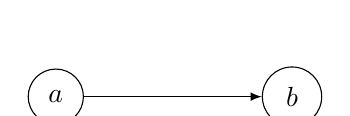
\begin{tikzpicture}
\draw (0,0) \relnode{a}{$a$} ;
\draw (3,0) \relnode{b}{$b$} ;
\draw[-latex] (a) -- (b) ;
\end{tikzpicture}
\end{center}

A \textit{reflexive} relation is one that relates every element of its domain to itself.

\begin{definition}
\label{defReflexiveRelation}
\index{reflexive relation}
\index{relation!reflexive}
A relation $R$ on a set $X$ is \textbf{reflexive} if $a \mathrel{R} a$ for all $a \in X$.
\end{definition}

\begin{center}
\begin{tikzpicture}
\draw (0,0) \relnode{a}{$a$} ;
\draw[-latex] (a) to[loop] (a) ;
\end{tikzpicture}
\end{center}

\begin{example}
\label{exEqualityIsReflexive}
Given any set $X$, the equality relation $=$ on $X$ is reflexive, since $a = a$ for all $a \in X$.
\end{example}

\begin{example}
\label{exDifferenceOfRealsInQIsReflexive}
%% BEGIN EXTRACT %%
Let $R$ be the relation on $\mathbb{R}$ defined for $a,b \in \mathbb{R}$ by $a \mathrel{R} b$ if and only if $b-a \in \mathbb{Q}$. Then $R$ is reflexive, since for all $a \in \mathbb{R}$, we have $a-a = 0 \in \mathbb{Q}$, so that $a \mathrel{R} a$.
%% END EXTRACT %%
\end{example}

\begin{exercise}
\label{exSubsetIsReflexive}
Let $X$ be a set. Prove that $\subseteq$ is a reflexive relation on $\mathcal{P}(X)$, but $\subsetneqq$ is not.
\end{exercise}

\begin{exercise}
\label{exDivisibilityIsReflexive}
Prove that the relation `$x$ divides $y$' on $\mathbb{Z}$ is reflexive.
\end{exercise}

The next exercise demonstrates that when determining if a relation is reflexive, we must be careful to specify its domain.

\begin{exercise}
\label{exReflexivitySensitiveToDomainOfRelation}
Let $G = \{ (1,1), (2,2), (3,3) \}$. Let $R$ be the relation on $[3]$ whose graph is $G$, and let $S$ be the relation on $[4]$ whose graph is $G$. Prove that $R$ is reflexive, but $S$ is not.
\end{exercise}

Symmetric relations are those for which the \textit{direction} of the relation doesn't matter: two elements are either each related to the other, or not related at all.

\begin{definition}
\label{defSymmetricRelation}
\index{symmetric relation}
\index{relation!symmetric}
A relation $R$ on a set $X$ is \textbf{symmetric} if, for all $a,b \in X$, if $a \mathrel{R} b$, then $b \mathrel{R} a$.
\end{definition}

\begin{center}
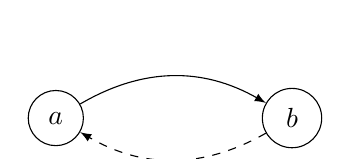
\begin{tikzpicture}
\draw (0,0) \relnode{a}{$a$} ;
\draw (3,0) \relnode{b}{$b$} ;
\draw[-latex] (a) to[bend left] (b) ;
\draw[-latex, dashed] (b) to[bend left] (a) ;
\end{tikzpicture}
\end{center}

\begin{example}
\label{exEqualityIsSymmetric}
Given any set $X$, the equality relation $=$ on $X$ is symmetric, since for all $a,b \in X$, if $a=b$, then $b=a$.
\end{example}

\begin{example}
\label{exDifferenceOfRealsInQIsSymmetric}
Let $R$ be the relation on $\mathbb{R}$ defined for $a,b \in \mathbb{R}$ by $a \mathrel{R} b$ if and only if $b-a \in \mathbb{Q}$. Then $R$ is symmetric.

To see this, let $a,b \in \mathbb{R}$ and assume that $a \mathrel{R} b$. Then $b-a \in \mathbb{Q}$, so that $b-a = \dfrac{p}{q}$ for some $p,q \in \mathbb{Z}$ with $q \ne 0$. But then
\[ a-b = -(b-a) = \dfrac{-p}{q} \]
so that $a-b \in \mathbb{Q}$. Hence $b \mathrel{R} a$, as required.
\end{example}

\begin{exercise}
Find all subsets $U \subseteq \mathbb{Z}$ such that the relation `$x$ divides $y$' on $U$ is symmetric.
\end{exercise}

We showed in \Cref{exReflexivitySensitiveToDomainOfRelation} that reflexivity of a relation is sensitive to its domain. The next exercise demonstrates that symmetry is \textit{not} sensitive to the domain---that is, it is an \textit{intrinsic} property of the relation.

\begin{exercise}
\label{exSymmetryNotSensitiveToDomainOfRelation}
Let $R$ and $S$ be relations such that $\mathrm{Gr}(R) = \mathrm{Gr}(S)$. Note that the domain of $R$ might be different from the domain of $S$. Prove that $R$ is symmetric if and only if $S$ is symmetric.
\end{exercise}

A condition related to symmetry, but in a sense opposite to it, is \textit{antisymmetry}. It says that the only way that two elements of a set can each be related to the other is if they are equal.

\begin{definition}
\index{antisymmetric relation}
\index{relation!antisymmetric}
Let $X$ be a set. A relation $R$ on $X$ is \textbf{antisymmetric} if, for all $a,b \in X$, if $a \mathrel{R} b$ and $b \mathrel{R} a$, then $a=b$.
\end{definition}

\begin{center}
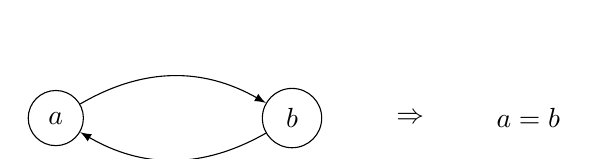
\begin{tikzpicture}
\draw (0,0) \relnode{a}{$a$} ;
\draw (3,0) \relnode{b}{$b$} ;
\draw[-latex] (a) to[bend left] (b) ;
\draw[-latex] (b) to[bend left] (a) ;
\draw (4.5,0) node {$\Rightarrow$} ;
\draw (6,0) node {$a=b$} ;
\end{tikzpicture}
\end{center}

A word of warning here is that `antisymmetric' does not mean the same thing as `not symmetric'---indeed, we we will see, equality is both symmetric and antisymmetric, and many relations are neither symmetric nor antisymmetric. [Even more confusingly, there is a notion of \textit{asymmetric relation}, which also does not mean `not symmetric'.]

\begin{example}
Given any set $X$, the equality relation $=$ on $X$ is antisymmetric, since for all $a,b \in X$, if $a=b$ and $b=a$, then $a=b$.
\end{example}

\begin{example}
The order relation $\le$ on $\mathbb{R}$ is antisymmetric, since for all $a,b \in \mathbb{R}$, if $a \le b$ and $b \le a$, then $a=b$.
\end{example}

\begin{exercise}
\label{exDivisibilityIsOrIsNotAntisymmetric}
Prove that the relation `$x$ divides $y$' on $\mathbb{N}$ is antisymmetric, but not on $\mathbb{Z}$.
\end{exercise}

\begin{exercise}
Let $X$ be a set. Prove that $\subseteq$ is an antisymmetric relation on $\mathcal{P}(X)$.
\end{exercise}

\begin{exercise}
Let $X$ be a set and let $R$ be a relation on $X$. Prove that $R$ is both symmetric and antisymmetric if and only if $\mathrm{Gr}(R) \subseteq \Delta_X$, where $\Delta_X$ is the diagonal subset of $X \times X$ (see \Cref{defDiagonalSubset}). Deduce that the only reflexive, symmetric and antisymmetric relation on a set $X$ is the equality relation on $X$.
\end{exercise}

The last property we will study in some detail is \textit{transitivity}. Transitive relations are those for which we can skip over intermediate related elements---for example, we can deduce $0 < 3$ from the facts that $0 < 1$ and $1 < 2$ and $2 < 3$.

\begin{definition}
\label{defTransitiveRelation}
\index{relation!transitive}
\index{transitive relation}
A relation $R$ on a set $X$ is \textbf{transitive} if, for all $a,b,c \in X$, if $a \mathrel{R} b$ and $b \mathrel{R} c$, then $a \mathrel{R} c$.
\end{definition}

\begin{center}
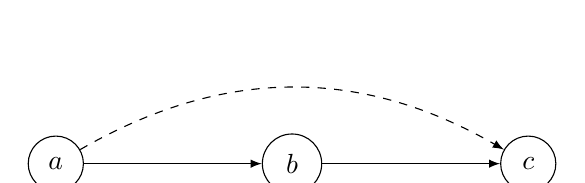
\begin{tikzpicture}
\draw (0,0) \relnode{a}{$a$} ;
\draw (3,0) \relnode{b}{$b$} ;
\draw (6,0) \relnode{c}{$c$} ;
\draw[-latex] (a) to (b) ;
\draw[-latex] (b) to (c) ;
\draw[-latex, dashed] (a) to[bend left] (c) ;
\end{tikzpicture}
\end{center}

\begin{example}
\label{exEqualityIsTransitive}
Given any set $X$, the equality relation $=$ on $X$ is transitive since, for all $a,b,c \in X$, if $a=b$ and $b=c$, then $a=c$.
\end{example}

\begin{example}
\label{exDifferenceOfRealsInQIsTransitive}
Let $R$ be the relation on $\mathbb{R}$ defined for $a,b \in \mathbb{R}$ by $a \mathrel{R} b$ if and only if $b-a \in \mathbb{Q}$. Then $R$ is transitive.

To see this, let $a,b,c \in \mathbb{R}$ and assume that $a \mathrel{R} b$ and $b \mathrel{R} c$. Then $b-a \in \mathbb{Q}$ and $c-b \in \mathbb{Q}$, so there exist $p,q,r,s \in \mathbb{Z}$ with $q,s \ne 0$ such that
\[ b-a = \dfrac{p}{q} \quad \text{and} \quad c-b = \dfrac{r}{s} \]
It follows that 
\[ c-a = (c-b) + (b-a) = \dfrac{p}{q} + \dfrac{r}{s} = \dfrac{ps+qr}{qs} \]
so that $c-a \in \mathbb{Q}$. Hence $a \mathrel{R} c$, as required.
\end{example}

\begin{exercise}
Let $X$ be a set. Prove that $\subseteq$ is a transitive relation on $\mathcal{P}(X)$.
\end{exercise}

\begin{exercise}
\label{exDivisibilityIsTransitive}
Prove that the relation `$x$ divides $y$' on $\mathbb{Z}$ is transitive.
\end{exercise}

Like symmetry, transitive is an intrinsic property of relations---that is, transitivity is not sensitive to the domain of the relation---as the next exercise demonstrates.

\begin{exercise}
\label{exTransitivityNotSensitiveToDomainOfRelation}
Let $R$ and $S$ be relations such that $\mathrm{Gr}(R) = \mathrm{Gr}(S)$. Note that the domain of $R$ might be different from the domain of $S$. Prove that $R$ is transitive if and only if $S$ is transitive.
\end{exercise}

A fundamental property of transitive relations is that we can prove two elements $a$ and $b$ are related by finding a chain of related elements starting at $a$ and finishing at $b$. This is the content of the following proposition.

\begin{proposition}
\label{propTransitiveChain}
Let $R$ be a relation on a set $X$. Then $R$ is transitive if and only if, for any finite sequence $x_0, x_1, \dots, x_n$ of elements of $X$ such that $x_{i-1} \mathrel{R} x_i$ for all $i \in [n]$, we have $x_0 \mathrel{R} x_n$.
\end{proposition}
\begin{cproof}
For the sake of abbreviation, let $p(n)$ be the assertion that, for any $n \ge 1$ and any sequence $x_0, x_1, \dots, x_n$ of elements of $X$ such that $x_{i-1} \mathrel{R} x_i$ for all $i \in [n]$, we have $x_0 \mathrel{R} x_n$.

We prove the two directions of the proposition separately.
\begin{itemize}
\item ($\Rightarrow$) Suppose $R$ is transitive. For $n \ge 1$. We prove $p(n)$ is true for all $n \ge 1$ by induction.
\begin{itemize}
\item (\textbf{Base case}) When $n=1$ this is immediate, since we assume that $x_0 \mathrel{R} x_1$.
\item (\textbf{Induction step}) Fix $n \ge 1$ and suppose $p(n)$ is true. Let $x_0, \dots, x_n, x_{n+1}$ is a sequence such that $x_{i-1} \mathrel{R} x_i$ for all $i \in [n+1]$. We need to prove that $x_0 \mathrel{R} x_{n+1}$.

By the induction hypothesis we know that $x_0 \mathrel{R} x_n$. By definition of the sequence we have $x_n \mathrel{R} x_{n+1}$. By transitivity, we have $x_0 \mathrel{R} x_{n+1}$.
\end{itemize}
So by induction, we have proved the $\Rightarrow$ direction.
\item ($\Leftarrow$)
%% BEGIN EXTRACT (xtrSubstitutionExample) %%
Suppose $p(n)$ is true for all $n \ge 1$. Then in particular $p(2)$ is true, which is precisely the assertion that $R$ is transitive.
%% END EXTRACT %%
\end{itemize}
So we're done.
\end{cproof}

That is, \Cref{propTransitiveChain} states that for a transitive relation $R$ on a set $X$, if $x_0, x_1, \dots, x_n \in X$, then
\[ x_0 \mathrel{R} x_1 \mathrel{R} \cdots \mathrel{R} x_n \quad \Rightarrow \quad x_0 \mathrel{R} x_n \]
where `$x_0 \mathrel{R} x_1 \mathrel{R} \cdots  \mathrel{R} x_n$' abbreviates the assertion that $x_i \mathrel{R} x_{i+1}$ for each $i < n$.

\index{relation|)}

\newpage
% !TeX root = ../../book.tex
\section{Equivalence relations and partitions}
\secbegin{secEquivalenceRelationsPartitions}
\index{equivalence relation|(}
\index{relation!equivalence relation|(}

An equivalence relation on a set $X$ is a relation on $X$ that, to a certain extent, \textit{behaves like equality}. That is, equivalence relations give us a way of saying that two elements of a set are `similar', without having to be equal. As an example, we might be interested in when the base-10 expansions of two natural numbers end in the \textit{same} digit, or when two finite sets have the \textit{same} number of elements.

\begin{definition}
\label{defEquivalenceRelation}
\index{relation!equivalence relation}
\index{equivalence relation}
A relation $R$ on a set $X$ is an \textbf{equivalence relation} if it is reflexive, symmetric and transitive.
\end{definition}

To denote a relation that we know (or suspect) is an equivalence relation, we will usually use a symbol like `$\sim$' \inlatex{sim}\lindexmmc{sim}{$\sim$} or `$\equiv$' \inlatex{equiv}\lindexmmc{equiv}{$\equiv$} or `$\approx$' \inlatex{approx}\lindexmmc{approx}{$\approx$} instead of a letter like `$R$' or `$S$'.
\nindex{eqrel}{$\sim$, $\equiv$, $\approx$}{equivalence relation}

\begin{example}
\label{exEqualityIsEquivalenceRelation}
Given any set $X$, it follows from \Cref{exEqualityIsReflexive,exEqualityIsSymmetric,exEqualityIsTransitive} that the equality relation $=$ is an equivalence relation on $X$. This is a relief, since we motivated equivalence relations by saying that they are those that behave like equality!
\end{example}

\begin{example}
\label{exDifferenceOfRealsInQIsEquivalenceRelation}
Let $R$ be the relation on $\mathbb{R}$ defined for $a,b \in \mathbb{R}$ by $a \mathrel{R} b$ if and only if $b-a \in \mathbb{Q}$. Piecing together \Cref{exDifferenceOfRealsInQIsReflexive,exDifferenceOfRealsInQIsSymmetric,exDifferenceOfRealsInQIsTransitive}, we see that $R$ is an equivalence relation on $\mathbb{R}$.
\end{example}

\begin{exercise}
\label{exEquivalenceRelationFromFunction}
Given a function $f : X \to Y$, define a relation $\sim_f$ on $X$ by
\[ a \sim_f b \quad \Leftrightarrow \quad f(a) = f(b) \]
for all $a,b \in X$. Prove that $\sim_f$ is an equivalence relation on $X$.
\end{exercise}

The equivalence relation in the next exercise comes back with a vengeance in \Cref{secCardinality}, where we will use it to compare the sizes of (finite and) infinite sets.

\begin{exercise}
\label{exBijectionIsEquivalenceRelation}
Let $\mathcal{S}$ be some set whose elements are all sets. (For example, we could take $\mathcal{S} = \mathcal{P}(X)$ for some fixed set $X$.) Define a relation $\cong$ \inlatex{cong}\lindexmmc{cong}{$\cong$} on $\mathcal{S}$ by letting $U \cong V$ if and only if there exists a bijection $f : U \to V$, for all $U,V \in \mathcal{S}$. Prove that $\cong$ is an equivalence relation on $\mathcal{S}$.
\end{exercise}

\subsection*{A first look at modular arithmetic}

A particularly useful family of equivalence relations is given by \textit{congruence} of integers, which allows us to do \textit{modular arithmetic}---this is the topic of \Cref{secModularArithmetic}. For a fixed integer $n$, this relation identifies two integers when they have the same remainder upon division by $n$ (as in \Cref{thmDivisionPreliminary}).

\begin{restatable}{definition}{rdefCongruence}
\label{defCongruence}
\index{congruence}
\index{modulo}
\nindex{mod}{$a \equiv b \bmod n$}{congruence}
\nindex{mod2}{$\bmod$}{congruence}
\lindexmmc{not}{$\not\in, \not\equiv, \dots$}
\lindexmmc{bmod}{$\bmod$}
Fix $n \in \mathbb{Z}$. Given integers $a,b \in \mathbb{Z}$, we say $a$ is \textbf{congruent} to $b$ \textbf{modulo} $n$, and write
\[ a \equiv b \bmod{n} \text{ \inlatexnb{a \textbackslash{}equiv b \textbackslash{}bmod\{n\}}} \]
if $n$ divides $a-b$. If $a$ is not congruent to $b$ modulo $n$, write
\[ a \not \equiv b \bmod n \text{ \inlatex{not\textbackslash{}equiv}} \]
The number $n$ is called the \textbf{modulus} of the congruence.
\end{restatable}

Before we prove that congruence is modulo $n$ is an equivalence relation for all $n \in \mathbb{Z}$, it is worthwhile to get a feel for how it works.

\begin{example}
\label{exCongruenceModuloTwoIsSameAsParity}
Let $a,b \in \mathbb{Z}$. Then $a \equiv b \bmod 2$ if and only if $a$ and $b$ are both even or both odd---that is, if and only if they have the same \textit{parity}.

Indeed, by the division theorem, we can write $a=2k+i$ and $b=2\ell+j$ for some $k,\ell \in \mathbb{Z}$ and $i,j \in \{ 0,1 \}$. Then
\[ b - a ~=~ (2k+i) - (2\ell+j) ~=~ 2(k-\ell) + (i-j) \]
Note that $i-j \in \{ {-1},0,1 \}$, and so $a \equiv b \bmod 2$ if and only if $i=j$. But this occurs if and only if $i=j=0$, in which case $a$ and $b$ are both even, or $i=j=1$, in which case $a$ and $b$ are both odd.
\end{example}

\begin{example}
\label{exModuloTenIsSameAsLastDigit}
Let $a,b \in \mathbb{N}$. Then $a \equiv b \bmod{10}$ if and only if $10$ divides $b-a$, which occurs if and only if the last digit in the decimal expansion of $b-a$ is $0$. But this implies that the decimal expansions of $a$ and $b$ have the same last digit. So the relation of congruence modulo $10$ on $\mathbb{N}$ is the same as the relation of `having the same last (decimal) digit'.
\end{example}

\begin{exercise}
Let $n \in \mathbb{Z}$. Prove that if $n \ne 0$, then $a \equiv b \bmod n$ if and only if $a$ and $b$ have the same remainder when divided by $n$.
\end{exercise}

\begin{exercise}
Let $a,b \in \mathbb{Z}$. When is it true that $a \equiv b \bmod 0$? When is it true that $a \equiv b \bmod 1$?
\end{exercise}

Having got a better feel for how congruence works, we now prove that, for each $n \in \mathbb{Z}$, congruence modulo $n$ is an equivalence relation on $\mathbb{Z}$.

\begin{restatable}{theorem}{rthmCongruenceIsEquivalenceRelation}
\label{thmCongruenceIsEquivalenceRelation}
Let $n \in \mathbb{Z}$. Then congruence modulo $n$ is an equivalence relation on $\mathbb{Z}$. That is:
\begin{enumerate}[(a)]
\item $a \equiv a \bmod n$ for all $a \in \mathbb{Z}$;
\item For all $a,b \in \mathbb{Z}$, if $a \equiv b \bmod n$, then $b \equiv a \bmod n$;
\item For all $a,b,c \in \mathbb{Z}$, if $a \equiv b \bmod n$ and $b \equiv c \bmod n$, then $a \equiv c \bmod n$.
\end{enumerate}
\end{restatable}

\begin{cproof}
\fixlistskip
\begin{enumerate}[(a)]
\item Let $a \in \mathbb{Z}$. Note that $a-a=0$, which is divisible by $n$ since $0 = 0 \times n$, and hence $a \equiv a \bmod n$. So congruence modulo $n$ is reflexive.
\item Let $a,b \in \mathbb{Z}$ and suppose $a \equiv b \bmod n$. Then $n$ divides $a-b$, so that $a-b = kn$ for some $k \in \mathbb{Z}$. Hence $b-a=-kn$, and so $n$ divides $b-a$, so that $b \equiv a \bmod n$ as required. So congruence modulo $n$ is symmetric.
\item Let $a,b,c \in \mathbb{Z}$ and suppose that $a \equiv b \bmod n$ and $b \equiv c \bmod n$. Then $n$ divides both $a-b$ and $b-c$, so there exist $k, \ell \in \mathbb{Z}$ such that
\[ a-b = kn \quad \text{and} \quad b-c = \ell n \]
Hence $a-c = (a-b)+(b-c) = (k+\ell)n$, so that $n$ divides $a-c$. Hence $a \equiv c \bmod n$, as required. So congruence modulo $n$ is transitive.
\end{enumerate}
Since congruence modulo $n$ is reflexive, symmetric and transitive, it is an equivalence relation.
\end{cproof}

\subsection*{Equivalence classes}

What makes equivalence relations so useful is they give us a way of ignoring information that is irrelevant to the task at hand.

For example, suppose $a$ and $b$ are two very large natural numbers, each with several trillion (decimal) digits. We want to know what the last digit of $ab$ is. To find this out, it would be silly to compute $ab$ and then look at its last digit. Instead, we can observe that the last digit of a product of two integers depends only on the last digit of each integer---for example, $1527 \times 9502$ has the same last digit as $7 \times 2 = 14$. By using the equivalence relation `has the same last digit as', we are able to ignore the irrelevant information about $a$ and $b$---that is, all but one of their trillions of digits---and simplify the problem considerably.

To make this precise, we introduce the notion of an \textit{equivalence class}. For a set $X$ with an equivalence relation, the equivalence class of an element $a \in X$ will be the set of elements of $X$ that $a$ is equivalent to. By working with the \textit{equivalence classes} of elements of $X$, rather than the elements of $X$ themselves, we are able to regard two equivalent elements as being `the same'.

\begin{definition}
\index{equivalence class}
\index{quotient!of a set by an equivalence relation}
Let $X$ be a set and let $\sim$ be an equivalence relation on $X$. The $\sim$-\textbf{equivalence class} of an element $a \in X$ is the set $[a]_{\sim}$ \inlatexnb{[x]\_\{\textbackslash{}sim\}} defined by
\[ [a]_{\sim} = \left\{ x \in X \mid a \sim x \right\} \]
\nindex{equivalence class}{$[a]_{\sim}$}{equivalence class}%
The \textbf{quotient} of $X$ by $\sim$ is the set $X/{\sim}$\nindex{quotient}{$X/{\sim}$}{quotient} \inlatexnb{X/\{\textbackslash{}sim\}} of all $\sim$-equivalence classes of elements of $X$; that is
\[ X/{\sim} = \left\{ [a]_{\sim} \mid a \in X \right\} \]
\end{definition}

\begin{latextip}
Putting \texcode{\{}curly brackets\texcode{\}} around the command for a symbol like $\sim$ (\texcodebs{sim}) tells \LaTeX{} to consider the symbol \textit{as a symbol}, rather than as a connective. Compare the following:

\begin{center}
\begin{tabular}{cc}
\textit{\TeX{} code}                    & \textit{Output} \\
\texcode{X/\textbackslash{}sim = Y}     & $X/\sim = Y$   \\
\texcode{X/\{\textbackslash{}sim\} = Y} & $X/{\sim} = Y$
\end{tabular}
\end{center}
This is because, without braces, \LaTeX{} thinks you're saying `$X$-forward-slash is related to is equal to $Y$', which clearly makes no sense; putting braces around \texcodebs{sim} signifies to \LaTeX{} that the $\sim$ symbol is being considered as an object in its own right, rather than as a connective.
\end{latextip}

\begin{example}
\label{exEquivalenceClassesModuloTwo}
Let $\sim$ be the relation of congruence modulo $2$ on $\mathbb{Z}$. We showed in \Cref{exCongruenceModuloTwoIsSameAsParity} that, for all $a,b \in \mathbb{Z}$ we have $a \equiv b \bmod 2$ if and only if $a$ and $b$ have the same parity. But this means that, for all $[a]_{\sim}$ is the set of all integers with the same parity as $a$---that is:
\begin{itemize}
\item If $a$ is even, then $[a]_{\sim}$ is the set of all even integers; and
\item If $a$ is odd, then $[a]_{\sim}$ is the set of all odd integers.
\end{itemize}
It follows that $\mathbb{Z}/{\sim} = \{ [0]_{\sim}, [1]_{\sim} \} = \{ E, O \}$, where $E$ is the set of all even integers and $O$ is the set of all odd integers.
\end{example}

\begin{exercise}
Let $\approx$ be the relation of congruence modulo $10$ on $\mathbb{N}$. Describe the equivalence classes, and give an explicit expression of the quotient $\mathbb{N}/{\approx}$ in list notation.
\end{exercise}

\begin{example}
Let $f : X \to Y$ be a function, and let $\sim_f$ be the equivalence relation on $X$ that we defined in \Cref{exEquivalenceRelationFromFunction}. Given $a \in X$, we have
\[ [a]_{\sim_f} = \{ x \in X \mid a \sim_f x \} = \{ x \in X \mid f(a) = f(x) \} \]
Thus we have $[a]_{\sim_f} = f^{-1}[\{ f(a) \}]$.
\end{example}

\begin{exercise}
Let $f : X \to Y$ be a function. Prove that $f$ is injective if and only if each $\sim_f$-equivalence class has a unique element, where $\sim_f$ is the equivalence relation defined in \Cref{exEquivalenceRelationFromFunction}.
\end{exercise}

The next result demonstrates that an equivalence relation $\sim$ on a set $X$ `descends' to the equality relation $=$ on the quotient $X/{\sim}$. This means that if we would rather deal with equality than with the equivalence relation itself, then we may do so by working inside the quotient $X/{\sim}$ rather than in the set $X$.

\begin{theorem}
\label{thmEquivalenceRelationDescendsToEqualityOnQuotient}
Let $\sim$ be an equivalence relation on a set $X$. Then for all $a,b \in X$, we have $a \sim b$ if and only if $[a]_{\sim} = [b]_{\sim}$.
\end{theorem}

\begin{cproof}
The proof is an exercise in piecing together the properties of equivalence relations.

Fix $a, b \in X$.
\begin{itemize}
\item ($\Rightarrow$) Suppose $a \sim b$. We prove $[a]_{\sim} = [b]_{\sim}$ by double containment.
\begin{itemize}
\item ($\subseteq$) Let $x \in [a]_{\sim}$---then $a \sim x$. We are assuming that $a \sim b$, so that $b \sim a$ by symmetry, and so $b \sim x$ by transitivity. So $x \in [b]_{\sim}$.
\item ($\supseteq$) Let $x \in [b]_{\sim}$---then $b \sim x$. We are assuming that $a \sim b$, and so $a \sim x$ by transitivity. So $x \in [a]_{\sim}$.
\end{itemize}
We have shown by double containment that $[a]_{\sim} = [b]_{\sim}$.

\item ($\Leftarrow$) Assume $[a]_{\sim} = [b]_{\sim}$. We have $b \sim b$ by reflexivity, and so $b \in [b]_{\sim}$. But then $b \in [a]_{\sim}$, so that $a \sim b$, as required.
\end{itemize}

So $a \sim b$ if and only if $[a]_{\sim} = [b]_{\sim}$.
\end{cproof}

For congruence, special terminology and notation exists for equivalence classes and quotients.

\begin{definition}
\label{defCongruenceClass}
\index{congruence class}
\nindex{an}{$[a]_n$}{congruence class}
\nindex{ZnZ}{$\mathbb{Z}/n\mathbb{Z}$}{set of congruence classes modulo $n$}
Let $n \in \mathbb{Z}$. The \textbf{congruence class} of an integer $a$ modulo $n$ is defined by
\[ [a]_n ~=~ [a]_{\equiv \bmod n} ~=~ \{ x \in \mathbb{Z} \mid a \equiv x \bmod n \} \]
The set of all congruence classes modulo $n$ is denoted by
\[ \mathbb{Z}/n\mathbb{Z} ~=~ \mathbb{Z}/({\equiv \bmod n}) ~=~ \{ [a]_n \mid a \in \mathbb{Z} \} \]
\end{definition}

\begin{example}
Using the terminology of congruence classes, \Cref{exEquivalenceClassesModuloTwo} can be rephrased by saying that $\mathbb{Z}/2\mathbb{Z} = \{ [0]_2, [1]_2 \}$. Moreover, \Cref{thmEquivalenceRelationDescendsToEqualityOnQuotient} gives us a more succinct proof: for all $a \in \mathbb{Z}$, we have $a \equiv 0 \bmod 2$ if and only if $a$ is even, and $a \equiv 1 \bmod 2$ if and only if $a$ is odd. Therefore for all $a \in \mathbb{Z}$, we have $[a]_2 = [0]_2$ or $[a]_2 = [1]_2$, and so
\[ \mathbb{Z}/2\mathbb{Z} ~=~ \{ [a]_2 \mid a \in \mathbb{Z} \} ~=~ \{ [0]_2, [1]_2 \} \]
Additionally, $[0]_2$ is the set of all even integers and $[1]_2$ is the set of all odd integers.
\end{example}

The next exercise generalises the previous one, proving that congruence classes correspond with remainders.

\begin{exercise}
\label{exCongruenceClassesCorrespondWithRemainders}
Let $n \in \mathbb{Z}$ with $n \ne 0$. Prove that the function
\[ i : \{ 0,~ 1,~ \dots,~ |n|-1 \} \to \mathbb{Z}/n\mathbb{Z} \]
defined by $i(r) = [r]_n$ for all $0 \le r < |n|$ is a bijection.
\end{exercise}

\subsection*{Partitions}

A partition of a set $X$ is a way of breaking $X$ up into mutually disjoint subsets. They will be an immensely useful tool for counting how many elements a finite set has in \Cref{chCombinatorics}, and will reappear in \Cref{secCardinalArithmetic} for defining arithmetic operations with cardinal numbers.

\begin{restatable}{definition}{rdefPartition}
\label{defPartition}
\index{pairwise disjoint}
\index{disjoint!pairwise}
A \textbf{partition} of a set $X$ is a collection $\mathcal{U} = \{ U_i \mid i \in I \}$ of subsets of $X$ such that the following conditions hold:
\begin{enumerate}[(a)]
\item For each $i \in I$, the subset $U_i$ is inhabited;
\item The sets $U_i$ for $i \in I$ are \textbf{pairwise disjoint}---that is, $U_i \cap U_j$ is empty for all $i,j \in I$ with $i \ne j$;
\item $\bigcup_{i \in I} U_i = X$.
\end{enumerate}
\end{restatable}

Note that, by contraposition, condition (b) in \Cref{exConditionsForPartition} is equivalent to saying that for all $i,j \in I$, if $U_i \cap U_j$ is inhabited, then $i=j$---this is useful for verifying pairwise disjointness in proofs.

\begin{strategy}[Proving a family of subsets forms a partition]
\label{strProvingSubsetsFormPartition}
Let $X$ be a set. In order to prove a collection $\mathcal{U} \subseteq \mathcal{P}(X)$ is a partition of $X$, it suffices to prove:
\begin{enumerate}[(a)]
\item Each $U \in \mathcal{U}$ is inhabited;
\item For all $U, V \in \mathcal{U}$, if $U \cap V$ is inhabited, then $U=V$;
\item For all $a \in X$, there is some $U \in \mathcal{U}$ such that $a \in U$.
\end{enumerate}
\end{strategy}

\begin{example}
\label{exPartitionOfZIntoEvenAndOdd}
We can partition $\mathbb{Z}$ as $E \cup O$, where $E$ is the set of all even integers and $O$ is the set of all odd integers:
\begin{enumerate}[(a)]
\item $E$ and $O$ are inhabited, since $0 \in E$ and $1 \in O$.
\item The family $\{ E, O \}$ is pairwise disjoint if and only if $E \cap O$ is empty; and it is, since no integer can be both even and odd.
\item $E \cup O = \mathbb{Z}$ since every integer is either even or odd.
\end{enumerate}
\end{example}

\begin{example}
\label{exPartitionOfNIntoPairs}
The sets $\{ 2n, 2n+1 \}$ for $n \in \mathbb{N}$ form a partition of $\mathbb{N}$:
\begin{enumerate}[(a)]
\item $2n \in \{ 2n, 2n+1 \}$ for each $n \in \mathbb{N}$, so the sets are all inhabited.
\item Suppose that $m,n \in \mathbb{N}$ and that $\{ 2m, 2m+1 \} \cap \{ 2n, 2n+1 \}$ is inhabited. Note that $2m \ne 2n+1$ and $2n \ne 2m+1$ by the division theorem (\Cref{thmDivisionTheorem}), so either $2m=2n$ or $2m+1=2n+1$. But in both cases we see that $m=n$. Hence the sets $\{ 2n, 2n+1 \}$ for $n \in \mathbb{N}$ are pairwise disjoint. 
\item Given $a \in \mathbb{N}$, we have $a=2n+i$, where $n \in \mathbb{N}$ is the quotient of $a$ when divided by $2$, and where $i \in \{0,1\}$ is the remainder of $a$ when divided by $2$. But then $a \in \{ 2n, 2n+1 \}$. Thus $\bigcup_{n \in \mathbb{N}} \{ 2n, 2n+1 \} = \mathbb{N}$.
\end{enumerate}
\end{example}

\begin{exercise}
\label{exPreimagesFormPartition}
Let $f : X \to Y$ be a surjection, and define a collection $\mathcal{F}$ of subsets of $X$ by
\[ \mathcal{F} = \{ f^{-1}[\{b\}] \mid b \in Y \} \]
That is, $\mathcal{F}$ is the set of subsets of $X$ given by the preimages of individual elements of $Y$ under $f$. Prove that $\mathcal{F}$ is a partition of $X$. Where in your proof do you use surjectivity of $f$?
\end{exercise}

\begin{exercise}
\label{exConditionsForPartition}
Let $X$ be a set and let $\mathcal{U} = \{ U_i \mid i \in I \}$ be a family of inhabited subsets of $X$. Prove that $\mathcal{U}$ is a partition of $X$ if and only if for reach $a \in X$, there is a unique set $U_i \in \mathcal{U}$ with $a \in U_i$.
\end{exercise}

\begin{exercise}
\label{exQuotientIsPartition}
If $\sim$ be an equivalence relation on $X$, then $X/{\sim}$ is a partition $X$.
\end{exercise}

In fact, the converse of \Cref{exQuotientIsPartition} is also true, as we prove next.

\begin{proposition}
\label{propPartitionIsQuotientByEquivalenceRelation}
Let $X$ be a set and let $\mathcal{U}$ be a partition of $X$. Then $\mathcal{U}=X/{\sim}$ for a unique equivalence relation $\sim$ on $X$.
\end{proposition}

\begin{cproof}
Define a relation $\sim$ by
\[ x \sim y \quad \Leftrightarrow \quad \exists U \in \mathcal{U},\, x \in U \text{ and } y \in U \]
for all $x,y \in X$. That is, $x \sim y$ if and only if $x$ and $y$ are elements of the same set of the partition. We check that $\sim$ is an equivalence relation.
\begin{itemize}
\item \textbf{Reflexivity.} Let $x \in X$. Then $x \in U$ for some $U \in \mathcal{U}$ since $\bigcup_{U \in \mathcal{U}} U = X$. Hence $x \sim x$.
\item \textbf{Symmetry.} Let $x,y \in X$ and suppose $x \sim y$. Then there is some $U \in \mathcal{U}$ with $x \in U$ and $y \in U$. But then it is immediate that $y \sim x$.
\item \textbf{Transitivity.} Let $x,y,z \in X$ and suppose that $x \sim y$ and $y \sim z$. Then there exist $U,V \in \mathcal{U}$ with $x,y \in U$ and $y,z \in V$. Thus $y \in U \cap V$. Since $\mathcal{U}$ is a partition of $X$, its elements are pairwise disjoint; thus if $U \ne V$ then $U \cap V = \varnothing$. Hence $U=V$. Thus $x \in U$ and $z \in U$, so $x \sim z$.
\end{itemize}
The definition of $\sim$ makes it immediate that $X/{\sim} = \mathcal{U}$.

To prove that $\sim$ is the only such relation, suppose $\approx$ is another equivalence relation on $X$ for which $X/{\approx}=\mathcal{U}$. Then, given $x,y \in X$, we have:
\begin{align*}
x \sim y & \Leftrightarrow \exists U \in \mathcal{U},\, x \in U \wedge y \in U && \text{by definition of $\sim$} \\
& \Leftrightarrow \exists z \in X,\, x \in [z]_{\approx} \wedge y \in [z]_{\approx} && \text{since $\mathcal{U} = X/{\approx}$} \\
& \Leftrightarrow \exists z \in X,\, x \approx z \wedge y \approx z && \text{by definition of $[z]_{\approx}$} \\
& \Leftrightarrow x \approx y && \text{by symmetry and transitivity}
\end{align*}
So ${\sim} = {\approx}$.
\end{cproof}

\Cref{exQuotientIsPartition} and \Cref{propPartitionIsQuotientByEquivalenceRelation} prove that equivalence relations and quotients are essentially the same thing: the quotient of a set by an equivalence relation is a partition of the set, and every partition of a set is the quotient by a unique equivalence relation!

The following lemma can be skipped over without grave consequences---it is a technical result with an extremely fiddly proof, but we will use it at a couple of points later in the book. It says that, given two partitioned sets, if we can pair up the sets in the partition, and pair up the elements in each pair of paired-up partitions, then we can pair up the elements of each set.

\begin{lemma}
\label{lemBijectionBetweenPartitionAndComponentsInducesBijectionOfSets}
Let $X$ and $Y$ be sets, let $\{ U_i \mid i \in I \}$ be a partition of $X$ and let $\{ V_j \mid j \in J \}$ be a partition of $Y$. If there exists:
\begin{itemize}
\item A bijection $f : I \to J$; and
\item For each $i \in I$, a bijection $g_i : U_i \to V_{f(i)}$;
\end{itemize}
then there exists a bijection $h : X \to Y$.
\end{lemma}

\begin{cproof}
Given $a \in X$, let $i(a)$ be the unique element of $I$ such that $a \in X_{i(a)}$. Note that this is valid since $\{ X_i \mid i \in I \}$ is a partition of $X$. Likewise, given $b \in Y$, let $j(b)$ be the unique element of $J$ such that $b \in Y_{j(b)}$.

Define $h : X \to Y$ by $h(a) = g_{i(a)}(a)$ for all $a \in X$. This is well-defined since
\[ h(a) = g_{i(a)}(a) \in Y_{f(i(a))} \subseteq Y \]
This also shows that $j(h(a)) = f(i(a))$.

Now define $k : Y \to X$ by $k(b) = g_{f^{-1}(j(b))}^{-1}(b)$ for all $b \in Y$. Then $k$ is well-defined: indeed, $g_{f^{-1}(j(b))}$ is a function from $U_{f^{-1}(j(b))}$ to $V_{j(b)}$, and so
\[ k(b) = g_{f^{-1}(j(b))}^{-1}(b) \in U_{f^{-1}(j(b))} \subseteq X \]
This also shows that $i(k(b)) = f^{-1}(j(b))$.

Then $k$ is an inverse for $h$. To see this, let $a \in X$; then
\begin{align*}
k(h(a)) &= g_{f^{-1}(j(h(a)))}^{-1} (h(a)) && \text{by definition of $k$} \\
&= g_{f^{-1}(f(i(a)))}^{-1} (h(a)) && \text{since $j(h(a)) = f(i(a))$} \\
&= g_{i(a)}^{-1}(h(a)) && \text{since $f^{-1} \circ f = \mathrm{id}_I$} \\
&= g_{i(a)}^{-1}(g_{i(a)}(a)) && \text{by definition of $h$} \\
&= a && \text{since $g_{i(a)}^{-1} \circ g_{i(a)} = \mathrm{id}_{X_{i(a)}}$}
\end{align*}

A similarly tedious computation reveals that $h(k(b)) = b$ for all $b \in Y$:
\begin{align*}
h(k(b)) &= g_{i(k(b))}(k(b)) && \text{by definition of $h$} \\
&= g_{f^{-1}(j(b))}(k(b)) && \text{since $i(k(b)) = f^{-1}(j(b))$} \\
&= g_{f^{-1}(j(b))}(g_{f^{-1}(j(b))}^{-1}(b)) && \text{by definition of $k$} \\
&= b && \text{since $g_{f^{-1}(j(b))} \circ g_{f^{-1}(j(b))}^{-1} = \mathrm{id}_{Y_{j(b)}}$}
\end{align*}

So $k$ is an inverse for $h$, as required.
\end{cproof}

\begin{exercise}
\label{exBijectionOfQuotientsAndClassesInducesBijectionOfSets}
Let $X$ and $Y$ be sets, let $\sim$ be an equivalence relation on $X$ and let $\approx$ be an equivalence relation on $Y$. Assume that there is a bijection $p : X/{\sim} \to Y/{\approx}$, and for each equivalence class $E \in X/{\sim}$ there is a bijection $h_E : E \to p(E)$. Use \Cref{lemBijectionBetweenPartitionAndComponentsInducesBijectionOfSets} to prove that there is a bijection $h : X \to Y$.
\end{exercise}

\subsection*{The quotient function}

We will now show that equivalence relations on a set $X$ are essentially the same thing as \textit{surjections} from $X$ to another set.

\begin{definition}
\label{defQuotientFunction}
\index{function!quotient}
\index{quotient function}
Let $X$ be a set and let $\sim$ be an equivalence relation on $X$. The \textbf{quotient function} for $\sim$ is the function $q_{\sim} : X \to X/{\sim}$ defined by $q(a) = [a]_{\sim}$ for each $a \in X$. That is, the quotient function sends each element of $X$ to its $\sim$-equivalence class.
\end{definition}

\begin{example}
Recall that, given $a \in \mathbb{Z}$, we have $[a]_2 = [0]_2$ if $a$ is even, and $[a]_2 = [1]_2$ is $a$ is odd. Thus the quotient function $q_2 : \mathbb{Z} \to \mathbb{Z}/2\mathbb{Z}$ can be viewed as telling us the parity of an integer.
\end{example}

\begin{exercise}
Let $n \in \mathbb{Z}$ with $n \ne 0$. Describe the quotient function $q_n : \mathbb{Z} \to \mathbb{Z}/n\mathbb{Z}$ in terms of remainders.
\end{exercise}

\begin{exercise}
\label{exQuotientFunctionIsSurjective}
Let $\sim$ be an equivalence relation on a set $X$. Prove that the quotient function $q_{\sim} : X \to X/{\sim}$ is surjective.
\end{exercise}

The theorem we prove next can be viewed as the converse to \Cref{exQuotientFunctionIsSurjective}. It proves that every surjection `is' a quotient function, in the sense that given any surjection $p : X \to A$, we can view $A$ as a quotient of $X$ by a suitably-defined equivalence relation, and then $p$ `is' the corresponding quotient function.

\begin{theorem}
\label{thmEquivalenceRelationsSurjections}
Let $X$ be a set. Then for every set $A$ and every surjection $p : X \to A$, there exist a unique equivalence relation $\sim$ on $X$ and bijection $f : X/{\sim} \to A$ such that $f([x]) = p(x)$ for all $x \in X$.
\end{theorem}

\begin{cproof}
Let $A$ be a set and $p : X \to A$ be a surjection.
\begin{itemize}
\item (\textbf{Existence}) Define a relation $\sim$ on $X$ by $x \sim y$ if and only if $p(x) = p(y)$. Then $\sim$ is an equivalence relation by \Cref{exEquivalenceRelationFromFunction}.

Moreover, given $x \in X$, we have
\[ [x]_{\sim} = \{ y \in X \mid p(x) = p(y) \} = p^{-1}[\{p(x)\}] \]
So define $f : X/{\sim} \to A$ by letting $f([x]_{\sim}) = p(x)$. Then $f$ is well-defined, since if $[x]_{\sim} = [y]_{\sim}$ then $x \sim y$, so that $p(x)=p(y)$.

Furthermore, $f$ is a bijection:
\begin{itemize}
\item (\textbf{Injectivity}) Let $[x]_{\sim},[y]_{\sim} \in X/{\sim}$ and assume $f([x]_{\sim}) = f([y]_{\sim})$. Then $p(x)=p(y)$, so that $x \sim y$, and hence $[x]_{\sim} = [y]_{\sim}$.
\item (\textbf{Surjectivity}) Let $a \in A$. Since $p$ is a surjection, there is some $x \in X$ such that $p(x) = a$. But then $f([x]_{\sim}) = p(x) = a$.
\end{itemize}
So we have established that there exist an equivalence relation $\sim$ on $X$ and a bijection $f : X/{\sim} \to A$ such that $f([x]_{\sim}) = p(x)$ for all $x \in X$.

\item (\textbf{Uniqueness}) Suppose $\approx$ is another equivalence relation on $X$ and that $g : X/{\approx} \to A$ is a bijection such that $g([x]_{\approx}) = p(x)$ for all $x \in X$. We prove that ${\sim} = {\approx}$, and then that $g = f$, so that $\sim$ and $f$ are unique.

So let $x,y \in X$. Then
\begin{align*}
x \sim y
&\Leftrightarrow p(x) = p(y) && \text{by definition of $\sim$} \\
&\Leftrightarrow g([x]_{\approx}) = g([y]_{\approx}) && \text{by definition of $g$} \\
&\Leftrightarrow [x]_{\approx} = [y]_{\approx} && \text{since $g$ is bijective} \\
&\Leftrightarrow x \approx y && \text{by \Cref{exQuotientIsPartition}}
\end{align*}

It follows that ${\sim} = {\approx}$, and then for all $x \in X$ we have
\[ f([x]_{\sim}) = p(x) = g([x]_{\approx}) = g([x]_{\sim}) \]
so that $f=g$, as required.
\end{itemize}
\end{cproof}

In light of \Cref{thmEquivalenceRelationsSurjections}, we have now established the equivalence of three notions for a given set $X$:
\begin{center}
\begin{tikzcd}[row sep=huge, column sep=normal]
&
\begin{matrix} \text{equivalence relations} \\ \text{on } X \end{matrix}
\arrow[dl, <->]
\arrow[dr, <->]
& \\
\begin{matrix} \text{partitions} \\ \text{of } X \end{matrix}
\arrow[rr, <->, dashed]
&&
\begin{matrix} \text{surjections with} \\ \text{domain } X \end{matrix}
\end{tikzcd}
\end{center}

\begin{exercise}
Give an explicit description of the dashed arrow in the above diagram. That is, describe the correspondence between partitions of a set $X$ and surjections whose domain is $X$.
\hintlabel{exPartitionsSurjections}{%
Given a partition $\mathcal{U}$ of a set $X$, find a surjection $q : X \to \mathcal{U}$. Then prove that, for every surjection $p : X \to A$, there is a unique partition $\mathcal{U}_p$ of $X$ and a unique bijection $f : \mathcal{U}_p \to A$ such that, for all $U \in \mathcal{U}_p$, we have $p(x) = f(U)$ for all $x \in U$. The structure of the proof will be similar to that of \Cref{thmEquivalenceRelationsSurjections}.
}
\end{exercise}

\index{equivalence relation|)}
\index{relation!equivalence relation|)}

% Chapter exercises
\chexbegin{chRelations}
\begin{chapex}
For each of the following binary operations on $\mathbb{Z}$, determine whether it is: (i) associative, (ii) unital, (iii) commutative.
\begin{multicols}{2}
\begin{enumerate}[(a)]
\item $a \star b = ab$
\item $a \star b = ab + a + b$
\item $a \star b = a^b$
\item $a \star b = |b - a|$
\item $a \star b = a$
\item $a \star b = a + b + 1$
\end{enumerate}
\end{multicols}
\end{chapex}
\chexend

\part{Topics in pure mathematics}
\label{ptTopics}

\chapter{Number theory}
    \label{chNumberTheory}
    \renewcommand{\currentchapter}{05}

% !TeX root = ../../book.tex



\newpage
\section{Division}
\secbegin{secDivision}

This section introduces the notion of \textit{divisibility}. As we have already mentioned, it is not always the case that one integer can divide another. As you read through this section, note that we never use fractions; everything we do is \textit{internal} to $\mathbb{Z}$, and does not require that we `spill over' to $\mathbb{Q}$ at any point. This will help you when you study ring theory in the future, and is a good practice to mimic in your own work.

The following theorem, called the division theorem, is the crux of everything that is to follow.

\begin{theorem}[Division theorem]
\label{thmDivisionTheorem}
\index{division theorem}
Let $a,b \in \mathbb{Z}$ with $b \ne 0$. There exist unique $q,r \in \mathbb{Z}$ such that
\[ a = qb + r \quad \text{and} \quad 0 \le r < |b| \]
\end{theorem}

\begin{strategy*}
Let's look at the simple case when $a \ge 0$ and $b > 0$. We can always find $q,r$ such that $a=qb+r$, for example $q=0$ and $r=a$. Moreover, by increasing $q$ we can reduce $r$, since
\[ qb+r = (q+1)b + (r-b) \]
We will keep doing this until the `remainder' is as small as it can be without being negative. As an example, consider the case when $a=14$ and $b=5$. This procedure gives
\begin{align*}
14 &= 0 \times 5 + 14 && \\
&= 1 \times 5 + 9 && \\
&= 2 \times 5 + 4 && \leftarrow \text{least nonnegative remainder}\\
&= 3 \times 5 + (-1) && \\
&= \cdots
\end{align*}
This procedure shows that in this case we should take $q=2$ and $r=4$, since $14 = 2 \times 5 + 4$ and $0 \le 4 < |5|$.

We can show that such a descending sequence of remainders terminates using the well-ordering principle, and then we must argue that the quotient and remainder that we obtain are unique.
\end{strategy*}

\begin{cproof}
%% BEGIN EXTRACT (xtrWlogExampleTwo) %%
We may assume that $b>0$: if not, replace $b$ by $-b$ and $q$ by $-q$. We may also assume that $a \ge 0$. Otherwise, replace $a$ by $-a$, $q$ by $-(q+1)$ and $r$ by $b-r$.
%% END EXTRACT %%

Thus, what follows assumes that $a \ge 0$ and $b > 0$.

\begin{itemize}
\item \textbf{Existence.} We prove that such integers $q,r$ exist by the well-ordering principle. Namely, we define a sequence $(r_n)_{n \in \mathbb{N}}$ such that $a=nb+r_n$ and $r_0 > r_1 > r_2 > \cdots$, and use this sequence to find the values of $q,r$.

\begin{itemize}
\item Let $r_0=a$. Then $a=0b+r_0$, as required.
\item Suppose $r_n$ has been defined, and let $r_{n+1} = r_n-b$. Then
\begin{align*}
(n+1)b+r_{n+1} &= (n+1)b+r_n-b \\
&= nb + b + r_n - b \\
&= nb + r = a
\end{align*}
Since $b>0$, we must have $r_{n+1} < r_n$ for all $n$.
\end{itemize}

Let $R = \mathbb{N} \cap \{ r_n \mid n \in \mathbb{N} \}$. That is, $R$ is the set of terms of the sequence which are non-negative. Since $r_0 = a \ge 0$, we have that $r_0 \in R$ and hence $R$ is inhabited. By the well-ordering principle, $R$ has a least element $r_k$ for some $k \in \mathbb{N}$.

Define $q=k$ and $r=r_k$. By construction we have $a=qb+r$ and $r \ge 0$, so
%% BEGIN EXTRACT (xtrContradictionOneLineExample) %%
it remains to show that $r < b$. Well, if $r \ge b$ then $r-b \ge 0$, but $r-b=r_{k+1}$, so this would imply $r_{k+1} \in R$, contradicting minimality of $r$. Hence $r < b$%
%% END EXTRACT %%
, so $q,r$ are as required.

\item \textbf{Uniqueness.} Suppose $q',r'$ also satisfy $a=q'b+r'$ and $0 \le r' < b$. If we can show that $r'=r$ then this proves that $q=q'$: indeed, if $qb+r=q'b+r$ then we can subtract $r$ and then divide by $b$, since $b>0$.

First note that $q' \ge 0$. If $q'<0$ then $q' \le -1$, so
\[ a = q'b+r' \le -b+r' \]
and hence $r' \ge a+b \ge b$ since $a \ge 0$. This contradicts the assumption that $r<b$. So $q' \ge 0$.

Since $q' \ge 0$, we also know that $a=q'b+r_{q'}$, and hence $r' = r_{q'} \in R$. By minimality of $r$ we have $r \le r'$. It remains to show that $r = r'$. If not then $r<r'$. Thus
\[ qb+r = q'b+r' > q'b+r \quad \Rightarrow \quad qb > q'b \quad \Rightarrow \quad q > q' \]
and hence $q = q'+t$ for some $t \ge 1$. But then
\[ q'b+r' = a = qb+r = (q'+t)b+r = q'b+(tb+r) \]
so $r' = tb + r \ge b$, contradicting $r'<b$. So $r=r'$ as desired, and hence $q=q'$.
\end{itemize}

At long last, we are done.
\end{cproof}

\begin{definition}
\label{defQuotientRemainder}
\index{quotient!of numbers}
\index{remainder}
Let $a,b \in \mathbb{Z}$ with $b \ne 0$, and let $q,r$ be the unique integers such that
\[ a = qb+r \quad \text{and} \quad 0 \le r < |b| \]
We say $q$ is the \textbf{quotient} and $r$ is the \textbf{remainder} of $a$ divided by $b$.
\end{definition}

\begin{example}
Some examples of division include:
\[ 14 = 2 \times 5 + 4, \qquad -14 = -3 \times 5 + 1, \qquad 15 = 3 \times 5 + 0 \]
\end{example}

\begin{definition}
\label{defDivision}
\index{division}
\index{divisor}
\index{factor}
Let $a,b \in \mathbb{Z}$. We say $b$ \textbf{divides} $a$, or that $b$ is a \textbf{divisor} (or \textbf{factor}) of $a$, if there exists $q \in \mathbb{Z}$ such that $a=qb$. To denote the fact that $b$ divides $a$ we write $b \mid a$\nindex{division}{$a \mid b$}{division} \inlatex{mid}\lindexmmc{mid}{$\mid$}. For the negation $\neg (b \mid a)$ write $b \nmid a$ \inlatex{nmid}\lindexmmc{nmid}{$\nmid$}.
\end{definition}

Thus, when $b \ne 0$, saying $b \mid a$ is equivalent to saying that the remainder of $a$ divided by $b$ is $0$.

\begin{example}
$5$ divides $15$ since $15 = 3 \times 5$. However, $5$ does not divide $14$: we know that the remainder of $14$ divided by $5$ is $4$, not $0$---and it can't be both since we proved in the division theorem that remainders are unique!
\end{example}

\begin{exercise}
\label{exOneDivDivZero}
Show that if $a \in \mathbb{Z}$ then $1 \mid a$, $-1 \mid a$ and $a \mid 0$. For which integers $a$ does $a \mid 1$? For which integers $a$ does $0 \mid a$?
\end{exercise}

We now introduce the very basic notion of a \textit{unit}. This notion is introduced to rule out trivialities. Units become interesting when talking about general rings, but in $\mathbb{Z}$, the units are very familiar.

\begin{definition}\index{unit}
Let $u \in \mathbb{Z}$. We say $u$ is a \textbf{unit} if $u \mid 1$; that is, $u$ is a unit if there exists $v \in \mathbb{Z}$ such that $uv=1$.
\end{definition}

\begin{proposition}\label{propUnitsOfZ}
The only units in $\mathbb{Z}$ are $1$ and $-1$.
\end{proposition}
\begin{cproof}
First note that $1$ and $-1$ are units, since $1 \cdot 1 = 1$ and $(-1) \cdot (-1) = 1$. Now suppose that $u \in \mathbb{Z}$ is a unit, and let $v \in \mathbb{Z}$ be such that $uv=1$. Certainly $u \ne 0$, since $0v=0 \ne 1$. If $u>1$ or $u<-1$ then $v = \frac{1}{u} \not \in \mathbb{Z}$. So we must have $u \in \{ -1, 1 \}$.
\end{cproof}

\Cref{exOneDivDivZero} shows that $-1$, $0$ and $1$ are, from the point of view of divisibility, fairly trivial. For this reason, most of the results we discuss regarding divisibility will concern \textbf{nonzero nonunits}\index{nonzero nonunit}, i.e.\ all integers except $-1$, $0$ or $1$.

\subsection*{Greatest common divisors}

\begin{definition}\index{greatest common divisor}
\label{defGCD}
Let $a, b \in \mathbb{Z}$. An integer $d$ is a \textbf{greatest common divisor} of $a$ and $b$ if:
\begin{enumerate}[(a)]
\item $d \mid a$ and $d \mid b$;
\item If $q$ is another integer such that $q \mid a$ and $q \mid b$, then $q \mid d$.
\end{enumerate}
\end{definition}

\begin{example}
\label{exGCDsOfFourAndSix}
$2$ is a greatest common divisor of $4$ and $6$; indeed:
\begin{enumerate}[(a)]
\item $4 = 2 \times 2$, and $6 = 3 \times 2$, so $2 \mid 4$ and $2 \mid 6$;
\item Suppose $q \mid 4$ and $q \mid 6$. The divisors of $4$ are $\pm 1, \pm 2, \pm 4$ and the divisors of $6$ are $\pm 1$, $\pm 2$, $\pm 3$, $\pm 6$. Since $q$ divides both, it must be the case that $q \in \{ {-2}, {-1}, 1, 2 \}$; in any case, $q \mid 2$.
\end{enumerate}
Likewise, $-2$ is a greatest common divisor of $4$ and $6$.
\end{example}

\begin{exercise}
\label{exGCDofSixAndFifteen}
There are two greatest common divisors of $6$ and $15$; find both.
\begin{backhint}
\hintref{exGCDofSixAndFifteen}
Remember that negative integers can be greatest common divisors too.
\end{backhint}
\end{exercise}

We will now prove that greatest common divisors \textit{exist}---that is, any two integers have a greatest common divisor---and that they are \textit{unique up to sign}.

\begin{theorem}
\label{thmGCDsExist}
Every pair of integers $a,b$ has a greatest common divisor.
\end{theorem}
\begin{cproof}
First note that if $a=b=0$, then $0$ is a greatest common divisor for $a$ and $b$. Moreover, we may take $a,b$ to be non-negative, since divisibility is insensitive to sign. So suppose that $a, b \ge 0$ and that $a,b$ are not both zero.

Define a set $X \subseteq \mathbb{Z}$ by
\[ X = \{ au+bv \mid u,v \in \mathbb{Z},\ au+bv > 0 \} \]
That is, $X$ is the set of positive integers of the form $au+bv$.

$X$ is inhabited. To see this, note that $a^2 > 0$ or $b^2 > 0$ since $a \ne 0$ or $b \ne 0$, so letting $u=a$ and $v=b$ in the expression $au+bv$, we see that
\[ au+bv=a^2+b^2>0 \quad \Rightarrow \quad a^2+b^2 \in X \]
By the well-ordering principle, $X$ has a least element $d$, and by definition of $X$ there exist $u,v \in \mathbb{Z}$ such that $d = au+bv$.

We will prove that $d$ is a greatest common divisor for $a$ and $b$.
\begin{itemize}
\item $d \mid a$. If $a=0$, then this is immediate, so suppose that $a > 0$. Let $q,r \in \mathbb{Z}$ be such that \[ a=qd+r \qquad \text{and} \qquad 0 \le r < d \]
Now $a = a \cdot 1 + b \cdot 0$, so $a \in X$, and hence $d \le a$. Moreover
\[ r = a-qd = a-q(au+bv) = a(1-qu) + b(-qv) \]
If $r>0$ then this implies that $r \in X$; but this would contradict minimality of $d$, since $r < d$. So we must have $r=0$ after all.
\item $d \mid b$. The proof of this is identical to the proof that $d \mid a$.
\item Suppose $q$ is an integer dividing both $a$ and $b$. Then $q \mid au+bv$ by \Cref{exDivisibilityIsLinear}. Since $au+bv=d$, we have $q \mid d$.
\end{itemize}
So $d$ is a greatest common divisor of $a$ and $b$ after all.
\end{cproof}

\begin{exercise}
\label{exGCDUnique}
Let $a,b \in \mathbb{Z}$. If $d$ and $d'$ are two greatest common divisors of $a$ and $b$, then either $d=d'$ or $d=-d'$.
\begin{backhint}
\hintref{exGCDUnique}
Start by proving that $d$ and $d'$ must divide each other.
\end{backhint}
\end{exercise}

\begin{aside}
A consequence of \Cref{thmGCDsExist} and \Cref{exGCDUnique} is that every pair of integers has a unique non-negative greatest common divisor! Written symbolically, we can say
\[ \forall (a,b) \in \mathbb{Z} \times \mathbb{Z},\, \exists ! d \in \mathbb{Z},\, \begin{pmatrix} d \ge 0 \text{ and } d \text{ is a greatest} \\ \text{common divisor for $a$ and $b$} \end{pmatrix} \]
As discussed in \Cref{secFunctions}, since this is a formula of the form `for all \dots{} there exists a unique \dots{}', this defines a function $\mathrm{gcd} : \mathbb{Z} \times \mathbb{Z} \to \mathbb{Z}$. We won't explicitly refer to the fact that $\mathrm{gcd}$ is a function; rather, we'll just concern ourselves with its values, as in \Cref{ntnGCDFunction}.
\end{aside}

\Cref{exGCDUnique} justifies our use of the following notation to refer to greatest common divisors.

\begin{notation}
\label{ntnGCDFunction}
\nindex{gcd}{$\mathrm{gcd}$}{greatest common divisor}
Let $a,b \in \mathbb{Z}$. Denote by $\mathrm{gcd}(a,b)$ \inlatex{mathrm\{gcd\}}\lindexmmc{mathrm}{$\mathrm{Aa}, \mathrm{Bb}, \dots$} the (unique!) non-negative greatest common divisor of $a$ and $b$.
\end{notation}

\begin{example}
In \Cref{exGCDsOfFourAndSix}, we saw that both $2$ and $-2$ are greatest common divisors of $4$ and $6$. Using \Cref{ntnGCDFunction}, we can now write $\mathrm{gcd}(4,6)=2$.
\end{example}

\begin{exercise}
For each $n \in \mathbb{Z}$, let $D_n \subseteq \mathbb{Z}$ be the set of divisors of $n$. Prove that $D_a \cap D_b = D_{\mathrm{gcd}(a,b)}$ for all $a,b \in \mathbb{Z}$.
\end{exercise}

Our goal for the rest of this subsection is to investigate the behaviour of greatest common divisors, find out how to compute them, and look into the implications they have for solutions to certain kinds of equations.

\begin{theorem}
\label{thmGCDSubtractMultiple}
Let $a,b,q,r \in \mathbb{Z}$, and suppose that $a=qb+r$. Then
\[ \mathrm{gcd}(a,b) = \mathrm{gcd}(b,r) \]
\end{theorem}
\begin{cproof}
Let $d = \mathrm{gcd}(a,b)$. We check that $d$ satisfies the conditions required to be a greatest common divisor of $b$ and $r$.

Note that $d \mid a$ and $d \mid b$, so let $s,t \in \mathbb{Z}$ be such that $a=sd$ and $b=td$.
\begin{itemize}
\item $d \mid b$ by definition, and $d \mid r$ since
\[ r = a-qb = sd-qtd = (s-qt)d \]
\item Suppose $d' \mid b$ and $d' \mid r$; say $b = ud'$ and $r=vd'$ with $u,v \in \mathbb{Z}$. Then $d' \mid a$, since
\[ a = qb+r = qud'+vd' = (qu+v)d' \]
so $d' \mid d$ since $d = \mathrm{gcd}(a,b)$.
\end{itemize}
So $d$ is a greatest common divisor of $b$ and $r$. Since $d>0$, the result is shown.
\end{cproof}

Combined with the division theorem (\Cref{thmDivisionTheorem}), \Cref{thmGCDSubtractMultiple} gives a relatively fast algorithm for computing the greatest common divisor of two integers, known as the \textbf{Euclidean algorithm}.

\begin{strategy}[Euclidean algorithm]
\label{strEuclideanAlgorithm}
\index{Euclidean algorithm}
Let $a,b \in \mathbb{Z}$. To compute $\mathrm{gcd}(a,b)$, proceed as follows.
\begin{itemize}
\item Set $r_0 = |a|$ and $r_1 = |b|$.
\item Given $r_{n-2}$ and $r_{n-1}$, define $r_n$ to be the remainder of $r_{n-2}$ divided by $r_{n-1}$.
\item Stop when $r_n = 0$; then $r_{n-1} = \mathrm{gcd}(a,b)$.
\end{itemize}
\end{strategy}

\begin{example}
We will find the greatest common divisor of $148$ and $28$.
\begin{align*}
148 &= 5 \times 28 + 8 && \\
28 &= 3 \times 8 + 4 && \\
8 &= 2 \times \boxed{4} + 0 && \leftarrow \text{Stop!}
\end{align*}
Hence $\mathrm{gcd}(148, 28) = 4$. Here the sequence of remainders is given by:
\[ r_0=148, \quad r_1 = 28, \quad r_2 = 8, \quad r_3 = 4, \quad r_4 = 0 \]
\end{example}

\begin{example} \label{exGCD13115757}
The Euclidean algorithm works surprisingly quickly, even for relatively large numbers. Consider the problem of computing $\mathrm{gcd}(1311, 5757)$ for example:
\begin{align*}
5757 &= 4 \times 1311 + 513 && \\
1311 &= 2 \times 513 + 285 && \\
513 &= 1 \times 285 + 228 && \\
285 &= 1 \times 228 + 57 && \\
228 &= 4 \times \boxed{57} + 0 && \leftarrow \text{Stop!}
\end{align*}
Hence $\mathrm{gcd}(1311,5757) = 57$. Here the sequence of remainders is given by:
\[ r_0=5757, \quad r_1 = 1311, \quad r_2 = 513, \quad r_3 = 285, \quad r_4 = 228, \quad r_5 = 57, \quad r_6 = 0 \]
\end{example}

\begin{example}
Here's an example where one of the numbers is negative: we compute the value of $\mathrm{gcd}(-420, 76)$:
\begin{align*}
-420 &= (-6) \times 76 + 36 && \\
76 &= 2 \times 36 + 4 && \\
36 &= 9 \times \boxed{4} + 0 && \leftarrow \text{Stop!}
\end{align*}
Hence $\mathrm{gcd}(-420, 76) = 4$.
\end{example}

\begin{example}
\label{exGCDsofPairs}
Use the Euclidean algorithm to compute the greatest common divisors of the following pairs of integers
\[ (12, 9), \quad (100, 35), \quad (7125, 1300), \quad (1010, 101010), \quad (-4, 14) \]
\end{example}

The following theorem will be useful when we study modular arithmetic in \Cref{secModularArithmetic}; it is called a `lemma' for historical reasons, and is really an important result in its own right.

\begin{theorem}[B\'{e}zout's lemma]
\label{thmBezout}
Let $a,b,c \in \mathbb{Z}$, and let $d = \mathrm{gcd}(a,b)$. The equation
\[ ax+by = c \]
has a solution $(x,y) \in \mathbb{Z} \times \mathbb{Z}$ if and only if $d \mid c$.
\end{theorem}
\begin{cproof}
($\Rightarrow$) Write $a=a'd$ and $b=b'd$, for $a',b' \in \mathbb{Z}$. If there exist $x,y \in \mathbb{Z}$ such that $ax+by=c$, then 
\[ c = ax+by = a'dx+b'dy = (a'x+b'y)d \]
and so $d \mid c$.

($\Leftarrow$) Suppose $d \mid c$, and let $c=kd$ for some $k \in \mathbb{Z}$.

If $c=0$, then a solution is $x=y=0$. If $c<0$, then $ax+by=c$ if and only if $a(-x)+b(-y)=-c$; so we may assume that $c>0$.

%% BEGIN EXTRACT %%
We proved in \Cref{thmGCDsExist} that a greatest common divisor of $a$ and $b$ is a least element of the set
\[ X = \{ au+bv \mid u,v \in \mathbb{Z},\ au+bv > 0 \} \]
So let $u,v \in \mathbb{Z}$ be such that $au+bv=d$. Then
\[ a(ku) + b(kv) = k(au+bv) = kd = c \]
and so letting $x=ku$ and $y=kv$, we see that the equation $ax+by=c$ has a solution $(x,y) \in \mathbb{Z} \times \mathbb{Z}$.
%% END EXTRACT %%
\end{cproof}

B\'{e}zout's lemma completely characterises when the equation $ax+by=c$ has a solution. An easy generalisation of B\'{e}zout's lemma provides a complete characterisation of when solutions to \textbf{linear Diophantine equations}\index{Diophantine equation!linear}\index{linear Diophantine equation} exist, that is equations of the form
\[ ax+by=c \]
where $a,b,c \in \mathbb{Z}$. We will soon develop an algorithm for computing \textit{all} solutions to these equations.

\begin{example}
Here are some examples of applications of B\'{e}zout's lemma.
\begin{itemize}
\item Consider the equation $1311x+5757y=12963$. We computed in \Cref{exGCD13115757} that $\mathrm{gcd}(1311,5757) = 57$. But $57 \nmid 12963$ since $12963 = 227 \times 57 + 24$. By B\'{e}zout's lemma, the equation $1311x+5757y=12963$ has no integer solutions.
\item For fixed $z$, the equation $4u+6v=z$ has solutions exactly when $z$ is even, since $\mathrm{gcd}(4,6)=2$.
\item For fixed $a,b$, the equation $au+bv=0$ always has solution. Indeed, setting $u=b$ and $v=-a$ gives a solution; but we knew one had to exist since by \Cref{exOneDivDivZero} we know that $d \mid 0$ for all $d \in \mathbb{Z}$.
\end{itemize}
\end{example}

\begin{exercise}
\label{exSolutionsToLDEs}
Which of the following equations have solutions?
\begin{enumerate}[(a)]
\item $12u + 9v = -18$
\item $12u + 9v = 1$
\item $100u + 35v = 125$
\item $7125u + 1300v = 0$
\item $1010u + 101010v = 1010101010101010$
\item $14u - 4v = 12$
\end{enumerate}
\begin{backhint}
\hintref{exSolutionsToLDEs}
\Cref{exGCDsofPairs} would be a good starting point.
\end{backhint}
\end{exercise}

\subsection*{Coprimality}

\begin{definition}
\label{defCoprime}
\index{coprime}
\index{relatively prime}
Let $a,b \in \mathbb{Z}$. We say $a$ and $b$ are \textbf{coprime} (or \textbf{relatively prime}), and write $a \perp b$\nindex{coprime}{$\perp$}{coprime} \inlatex{perp}\lindexmmc{perp}{$\perp$} (read `$a$ is coprime to $b$'), if $\mathrm{gcd}(a,b) = 1$.
\end{definition}

\begin{example}
$4 \perp 9$. To see this, note that if $d \mid 4$ then $d \in \{ {-4}, {-2}, {-1}, 1, 2, 4 \}$, and if $d \mid 9$ then $d \in \{ {-9}, {-3}, {-1}, 1, 3, 9 \}$. Hence if $d \mid 4$ and $d \mid 9$, then $d = 1$ or $d = -1$. It follows that $\mathrm{gcd}(4,9)=1$.
\end{example}

\begin{exercise}
\label{exCoprimeTo15}
Which integers in the set $[15]$ are coprime to $15$?
\end{exercise}

\begin{proposition}
Let $a,b \in \mathbb{Z}$. The following are equivalent:
\begin{enumerate}[(1)] \setlength{\itemindent}{20pt}
\item $a$ and $b$ are coprime;
\item If $d \in \mathbb{Z}$ with $d \mid a$ and $d \mid b$, then $d$ is a unit.
\end{enumerate}
\end{proposition}
\begin{cproof} We prove that condition (1) implies condition (2), and vice versa.
\begin{itemize}
\item (1)$\Rightarrow$(2). Suppose $a$ and $b$ are coprime, and fix $d \in \mathbb{Z}$ with $d \mid a$ and $d \mid b$. Then $d \mid \mathrm{gcd}(a,b) = 1$, so $d$ is a unit.

\item (2)$\Rightarrow$(1). Suppose condition (2) above holds. We prove that $1$ satisfies the conditions required to be a greatest common divisor of $a$ and $b$. The fact that $1 \mid a$ and $1 \mid b$ is automatic; and the fact that if $d \mid a$ and $d \mid b$ implies $d \mid 1$ is precisely the condition (2) that we are assuming.
\end{itemize}

Hence the two conditions are equivalent.
\end{cproof}

\begin{exercise}
\label{exDivByGCDIsCoprime}
Let $a$ and $b$ be integers, not both zero, and let $d = \mathrm{gcd}(a,b)$. The integers $\frac{a}{d}$ and $\frac{b}{d}$ are coprime.
\end{exercise}

The following corollary is a specialisation of B\'{e}zout's lemma to the case when $a$ and $b$ are coprime.

\begin{corollary}
Let $a,b \in \mathbb{Z}$. The equation $au+bv=1$ has a solution if and only if $a$ and $b$ are coprime. Moreover, if $a$ and $b$ are coprime, then the equation $au+bv=z$ has a solution for all $z \in \mathbb{Z}$.
\end{corollary}

\begin{cproof}
By B\'{e}zout's lemma (\Cref{thmBezout}), the equation $au+bv=1$ has a solution if and only if $\mathrm{gcd}(a,b) \mid 1$. But the only positive divisor of $1$ is $1$, so a solution exists if and only if $\mathrm{gcd}(a,b) = 1$, which is precisely the assertion that $a$ and $b$ are coprime.

If $a$ and $b$ are coprime, then $1 = \mathrm{gcd}(a,b) \mid z$ for all $z \in \mathbb{Z}$. So by B\'{e}zout's lemma again, the equation $au+bv=z$ has a solution for all $z \in \mathbb{Z}$.
\end{cproof}

A useful consequence of B\'{e}zout's lemma is the following result:

\begin{proposition}
\label{propADividesBC}
Let $a,b,c \in \mathbb{Z}$. If $a$ and $b$ are coprime and $a \mid bc$, then $a \mid c$.
\end{proposition}

\begin{cproof}
By B\'{e}zout's lemma (\Cref{thmBezout}) there exist integers $u$ and $v$ such that $au+bv=1$. Multiplying by $c$ gives $acu+bcv=c$. Since $a \mid bc$, we can write $bc=ka$ for some $k \in \mathbb{Z}$, and so $acu+kav=c$. But then \[ (cu+kv)a = c \] which proves that $a \mid c$.
\end{cproof}

\subsection*{Linear Diophantine equations}
\index{Diophantine equation!linear}
\index{linear Deiophantine equation}
We have now seen two important results:
\begin{itemize}
\item The \textbf{Euclidean algorithm}, which was a procedure for computing the greatest common divisor of two integers.
\item \textbf{B\'{e}zout's lemma}, which provides a necessary and sufficient condition for equations of the form $ax+by=c$ to have an integer solution.
\end{itemize}
We will now develop the \textbf{reverse Euclidean algorithm}\index{Euclidean algorithm!reverse}\index{reverse Euclidean algorithm}, which provides a method for computing a solutions to (bivariate) linear Diophantine equations, when such a solution exists. Then we will prove a theorem that characterises \textit{all} integer solutions in terms of a given solution.

\begin{example}
Suppose we want to find integers $x$ and $y$ such that $327x+114y=18$. Running the Euclidean algorithm yields that $\mathrm{gcd}(327,114)=3$ --- see below. For reasons soon to become apparent, we rearrange each equation to express the remainder on its own.
\begin{align*}
327 &= 2 \times 114 + 99 && \Rightarrow & 99 &= 327 - 2 \times 114 \tag{1} \\
114 &= 1 \times 99 + 15 && \Rightarrow & 15 &= 114 - 1 \times 99 \tag{2} \\
99 &= 6 \times 15 + 9 && \Rightarrow & \hspace{6pt}9 &= 99 - 6 \times 15 \tag{3} \\
15 &= 1 \times 9 + 6 && \Rightarrow & \hspace{6pt}6 &= 15 - 1 \times 9 \tag{4} \\
9 &= 1 \times 6 + 3 && \Rightarrow & \hspace{6pt}3 &= 9 - 1 \times 6 \tag{5} \\
6 &= 2 \times 3 + 0 && 
\end{align*}
We can then express $3$ in the form $327u+114v$ by successively substituting the equations into each other:
\begin{itemize}
\item Equation (5) expresses $3$ as a linear combination of $6$ and $9$. Substituting equation (4) yields:
\[ 3 = 9 - 1 \times (15 - 1 \times 9) \quad \Rightarrow \quad 3 = 2 \times 9 - 1 \times 15 \]
\item This now expresses $3$ as a linear combination of $9$ and $15$. Substituting equation (3) yields:
\[ 3 = 2 \times (99 - 6 \times 15) - 1 \times 15 \quad \Rightarrow \quad 3 = (-13)\times 15 + 2 \times 99 \]
\item This now expresses $3$ as a linear combination of $15$ and $99$. Substituting equation (2) yields:
\[ 3 = (-13)\times(114 - 1 \times 99) + 2 \times 99 \quad \Rightarrow \quad 3 = 15 \times 99 - 13 \times 114 \]
\item This now expresses $3$ as a linear combination of $99$ and $114$. Substituting equation (1) yields:
\[ 3 = 15 \times (327 - 2 \times 114) - 13 \times 114 \quad \Rightarrow \quad 3 = (-43) \times 114 + 15 \times 327 \]
\end{itemize}
Now that we've expressed $3$ as a linear combination of $114$ and $327$, we're nearly done: we know that $18 = 6 \times 3$, so multiplying through by $6$ gives
\[ 18 = (-258) \times 114 + 90 \times 327 \]
Hence $(x,y) = (90,{-258})$ is a solution to the equation $327x+114y=18$.
\end{example}

\begin{prooftip}
Let $a,b \in \mathbb{Z}$ and let $d = \mathrm{gcd}(a,b)$. To find integers $x,y$ such that $ax+by=d$:
\begin{enumerate}[(i)]
\item Run the Euclidean algorithm on the pair $(a,b)$, keeping track of all quotients and remainders.
\item Rearrange each equation of the form $r_{n-2} = q_nr_{n-1}+r_n$ to isolate $r_n$.
\item Substitute for the remainders $r_k$ in reverse order until $\mathrm{gcd}(a,b)$ is expressed in the form $ax+by$ for some $x,y \in \mathbb{Z}$.
\end{enumerate}
This process is called the \textbf{reverse Euclidean algorithm}.
\end{prooftip}

\begin{exercise}
Find a solution $(x,y) \in \mathbb{Z} \times \mathbb{Z}$ to the equation $630x + 385y = 4340$.
\end{exercise}

Now that we have a procedure for computing \textit{one} solution to the equation $ax+by=c$, we need to come up with a procedure for computing \textit{all} solutions. This can be done by proving the following theorem.

\begin{theorem}
\label{thmAllSolutionsOfLDEFromOneSolution}
Let $a,b,c \in \mathbb{Z}$, where $a$ and $b$ are not both zero. Suppose that $x_0$ and $y_0$ are integers such that $ax_0+by_0 = c$. Then, $(x,y) \in \mathbb{Z} \times \mathbb{Z}$ is another solution to the equation $ax+by=c$ if and only if
\[ x = x_0 + k \cdot \frac{b}{\mathrm{gcd}(a,b)} \qquad \text{and} \qquad y = y_0 - k \cdot \frac{a}{\mathrm{gcd}(a,b)} \]
for some $k \in \mathbb{Z}$.
\end{theorem}

Thus, as soon as we've found one solution $(x,y)=(x_0,y_0)$ to the equation $ax+by=c$, this theorem tells us what all other solutions must look like.

\begin{cproof}[of \Cref{thmAllSolutionsOfLDEFromOneSolution}]
We prove the two directions separately.

($\Rightarrow$). First suppose that $(x_0,y_0)$ is an integer solution to the equation $ax+by=c$. Let $k \in \mathbb{Z}$ and let
\[ x = x_0 + k \cdot \frac{b}{\mathrm{gcd}(a,b)} \qquad \text{and} \qquad y = y_0 - k \cdot \frac{a}{\mathrm{gcd}(a,b)} \]
Then
\begin{align*}
& ax+by && \\
&= a \left( x_0 + k \cdot \frac{b}{\mathrm{gcd}(a,b)} \right) + b \left( y_0 - k \cdot \frac{a}{\mathrm{gcd}(a,b)} \right) && \text{by definition of $x$ and $y$} \\
&= (ax_0 + by_0) + ak \cdot \frac{b}{\mathrm{gcd}(a,b)} - kb \cdot \frac{a}{\mathrm{gcd}(a,b)} && \text{rearranging} \\
&= (ax_0 + by_0) + \frac{kab-kab}{\mathrm{gcd}(a,b)} && \text{combining the fractions} \\
&= ax_0 + by_0 && \text{since $kab-kab=0$} \\
&= c && \text{since $(x_0,y_0)$ is a solution}
\end{align*}
so $(x,y)$ is indeed a solution to the equation.

($\Leftarrow$). First suppose that $a \perp b$. Fix a solution $(x_0,y_0)$ to the equation $ax+by=c$, and let $(x,y)$ be another solution. Then
\[ a(x-x_0) + b(y-y_0) = (ax_0 + by_0) - (ax+by) = c-c = 0 \]
so that
\[ a(x-x_0) = b(y_0-y) \]
Now $a$ and $b$ are coprime, so by \Cref{propADividesBC}, we have $a \mid y_0-y$ and $b \mid x-x_0$. Let $k,\ell \in \mathbb{Z}$ be such that $x-x_0=kb$ and $y_0-y = \ell a$. Then substituting into the above equation yields
\[ a \cdot k b = b \cdot \ell a \]
and hence $(k-\ell)ab = 0$. Since $ab \ne 0$, we have $k=\ell$, so that
\[ x = x_0 + kb \quad \text{and} \quad y = y_0-ka \]
Now we drop the assumption that $a \perp b$. Let $\mathrm{gcd}(a,b) = d \ge 1$. We know that $d \mid c$, by B\'{e}zout's lemma (\Cref{thmBezout}), and so 
\[ \frac{a}{d} x + \frac{b}{d} y = \frac{c}{d} \]
is another linear Diophantine equations, and moreover $\frac{a}{d} \perp \frac{b}{d}$ by \Cref{exDivByGCDIsCoprime}. By what we proved above, we have
\[ x = x_0 + k \cdot \frac{b}{d} \quad \text{and} \quad y=y_0-k \cdot \frac{a}{d} \]
for some $k \in \mathbb{Z}$. But this is exactly what we sought to prove!
\end{cproof}

\begin{example}
We know that $(x,y) = (90,{-258})$ is a solution to the equation $327x+114y=18$, and
\[ \displaystyle \frac{327}{\mathrm{gcd}(327,114)} = \frac{327}{3} = 109 \qquad \text{and} \qquad \displaystyle \frac{114}{\mathrm{gcd}(327,114)} = \frac{114}{3} = 38 \]
so this theorem tells us that $(x,y) \in \mathbb{Z} \times \mathbb{Z}$ is a solution to the equation $327x+114y=18$ if and only if
\[ x = 90 + 38k \qquad \text{and} \qquad y = -258-109k \]
for some $k \in \mathbb{Z}$.
\end{example}

\begin{exercise}
Find all integers $x,y$ such that
\[ 630x + 385y = 4340 \]
\end{exercise}

\subsection*{Least common multiples}

You would be forgiven for wondering why so much of the foregoing section was devoted to greatest common divisors, with no mention of least common multiples. We will now give the latter some attention.

\begin{definition}
\label{defLCM}
\index{least common multiple}
Let $a, b \in \mathbb{Z}$. An integer $m$ is a \textbf{least common multiple} of $a$ and $b$ if:
\begin{enumerate}[(a)]
\item $a \mid m$ and $b \mid m$;
\item If $c$ is another integer such that $a \mid c$ and $b \mid c$, then $m \mid c$.
\end{enumerate}
\end{definition}

The definition of least common multiple is \textit{dual} to that of greatest common divisor (\Cref{defGCD}). This means that many properties of greatest common divisors have corresponding `dual' properties, which hold of least common multiples. As such, we will not say much here about least common multiples, and that which we \textit{do} say is in the form of exercises.

\begin{exercise}
\label{exLCMExistsUnique}
Let $a,b \in \mathbb{Z}$. Prove that $a$ and $b$ have a least common multiple. Furthermore, prove that least common multiples are unique up to sign, in the sense that if $m,m'$ are two least common multiples of $a$ and $b$, then $m=m'$ or $m=-m'$.
\begin{backhint}
\hintref{exLCMExistsUnique}
This is essentially the same as \Cref{exGCDUnique}.
\end{backhint}
\end{exercise}

As with greatest common divisors, \Cref{exLCMExistsUnique} justifies the following definition.

\begin{definition}
\label{defLCMFunction}
Given $a,b \in \mathbb{Z}$, denote by $\mathrm{lcm}(a,b)$\nindex{lcm}{$\mathrm{lcm}$}{least common multiple} \inlatex{mathrm\{lcm\}}\lindexmmc{mathrm}{$\mathrm{Aa}, \mathrm{Bb}, \dots$} the non-negative least common multiple of $a$ and $b$.
\end{definition}

\begin{exercise}
\label{exProductOfIntegersIsProductOfGCDAndLCM}
Let $a,b \in \mathbb{Z}$. Prove that $\mathrm{gcd}(a,b) \cdot \mathrm{lcm}(a,b) = |ab|$.
\begin{backhint}
\hintref{exProductOfIntegersIsProductOfGCDAndLCM}
Define $m = \dfrac{ab}{\mathrm{gcd}(a,b)}$ and prove that $m$ satisfies the definition of being a least common multiple of $a$ and $b$ (\Cref{defLCM}). Then apply \Cref{exLCMExistsUnique}.
\end{backhint}
\end{exercise}

\newpage
\section{Prime numbers}
\secbegin{secPrimes}

Thinking of divisibility as a way of \textit{breaking down} an integer, for example $12 = 2 \times 2 \times 3$, our goal now is to show that there are particular integers that are \textit{atomic}---they are the building blocks of the integers, in the sense that:
\begin{itemize}
\item Every integer can be broken into a product of these atomic integers\dots{}
\item \dots{}and these atomic integers cannot themselves be broken down any further\dots{}
\item \dots{}\textit{and} there is an essentially unique way to write an integer as a product of these atomic integers.
\end{itemize}

There are a couple of fairly vague terms used here: `atomic' and `essentially unique'. But as always, we will make these terms precise when we need to.

\subsection*{Primes and irreducibles}

There are two ways that we might want to characterise the so-called \textit{atomic} integer that we just mentioned.
\begin{itemize}
\item One way that an integer might be atomic is if it allows us to break down products of integers---this leads to the notion of \textit{prime} (\Cref{defPrime}).
\item Another way is that an integer might be atomic is if it cannot be split up as a product of more than one integer (in a nontrivial way)---this leads to the notion of \textit{irreducible} (\Cref{defReducible}).
\end{itemize}
Conveniently, as we will show in \Cref{thmPrimeIffIrred}, these two notions coincide. But the fact that they coincide is not obvious, and uses essential properties of the integers that do not hold in more general structures.

The definition of \textit{prime} that we are about to give comes from abstract algebra (specifically, from ring theory). It might seem strange, but we will soon be able to show that the more familiar definition---that is, having exactly two positive divisors---is equivalent to this one.

\begin{definition}
\label{defPrime}
\index{prime}
An integer $p$ is (\textbf{ring theoretically}) \textbf{prime} if $p$ is a nonzero nonunit and, for all $a,b \in \mathbb{Z}$, if $p \mid ab$ then $p \mid a$ or $p \mid b$.
\end{definition}

\begin{example}
$2$ is prime. To see this, suppose it isn't. Then there exist $a,b \in \mathbb{Z}$ such that $2 \mid ab$ but $2$ divides neither $a$ nor $b$. Thus $a$ and $b$ are both odd, meaning that $ab$ is odd\dots{} but this contradicts the assumption that $2 \mid ab$.

However, $18$ is not prime. Indeed, $18 \mid 12 \times 15$ but $18$ divides neither $12$ nor $15$.
\end{example}

\begin{exercise}
Using \Cref{defPrime}, prove that $3$ and $5$ are prime, and that $4$ is not prime.
\end{exercise}

\begin{example}
Let $k \in \mathbb{Z}$ with $0<k<5$. We'll show that $5 \mid \binom{5}{k}$.

Well, by \Cref{thmBinomAsFactorialByInduction} we know that
\[ 5! = \binom{5}{k}k!(5-k)! \]
By \Cref{defFactorialRecursive}, we have
\[ \underbrace{5 \times 4!}_{=5!} = \binom{5}{k} \times \underbrace{1 \times \cdots \times k}_{=k!} \times \underbrace{1 \times \cdots \times (5-k)}_{=(5-k)!} \]
Since $5$ is prime, it must divide one of the factors on the right-hand side of this equation. Thus, either $5$ divides $\binom{5}{k}$, or it divides $\ell$ for some $1 \le \ell \le k$ or $1 \le \ell \le 5-k$. But $k<5$ and $5-k<5$, so it cannot divide any of these values of $\ell$---if it did, it would imply $5 \le \ell \le k$ or $5 \le \ell \le 5-k$, which is nonsense. Hence $5$ must divide $\binom{5}{k}$.
\end{example}

\begin{exercise}
Let $p \in \mathbb{Z}$ be a positive prime and let $0 < k < p$. Show that $p \mid \binom{p}{k}$.
\hintlabel{exPrimeDivBinomCoeff}{%
Use the factorial formula for binomial coefficients (\Cref{thmBinomAsFactorialByInduction}).
}
\end{exercise}

We now arrive at our second notion of \textit{atomic}, capturing the idea that it should not be possible to break an atomic integer into smaller parts.

\begin{definition}
\label{defReducible}
\index{irreducible number}
\index{reducible number}
An integer $a$ is \textbf{irreducible} if $a$ is a nonzero nonunit and, for all $m,n \in \mathbb{Z}$, if $a=mn$, then either $m$ or $n$ is a unit. Otherwise, $a$ is \textbf{reducible}.
\end{definition}

The notion of \textit{irreducible} captures more closely the more familiar notion of `prime', as the next result shows.

\begin{proposition}
\label{propFactorsOfIrred}
Let $p \in \mathbb{Z}$ be a nonzero nonunit. Then $p$ is irreducible if and only if the only divisors of $p$ are $p$, $-p$, $1$ and $-1$.
\end{proposition}
\begin{cproof}
Suppose $p$ is irreducible and that $a \mid p$. Then $p = ab$ for some $b \in \mathbb{Z}$. Since $p$ is irreducible, either $a$ or $b$ is a unit. If $a$ is a unit then $b = \pm p$, and if $b$ is a unit then $a = \pm p$. So the only divisors of $p$ are $\pm 1$ and $\pm p$.

Conversely, suppose that the only divisors of $p$ are $\pm 1$ and $\pm p$, and let $a,b \in \mathbb{Z}$ with $p=ab$. We want to prove that $a$ or $b$ is a unit. Since $a \mid p$, we have $a \in \{ 1, -1, p, -p \}$. If $a = \pm 1$, then $a$ is a unit; if $a=\pm p$, then $b = \pm 1$, so that $b$ is a unit. In any case, either $a$ or $b$ is a unit, and hence $p$ is irreducible.
\end{cproof}

\begin{example}
A couple of examples of reducible and irreducible numbers are:
\begin{itemize}
\item $2$ is irreducible: if $2=mn$ then either $m$ or $n$ is even, otherwise we'd be expressing an even number as the product of two odd numbers. We may assume $m$ is even, say $m=2k$; then $2=2kn$, so $kn=1$ and hence $n$ is a unit.
\item $20$ is reducible since $20 = 4 \times 5$ and neither $4$ nor $5$ is a unit.
\end{itemize}
\end{example}

\begin{exercise}
Let $p \in \mathbb{Z}$. Prove that if $p$ is ring theoretically prime, then $p$ is irreducible.
\hintlabel{exPrimeImpliesIrred}{%
Assume $p=mn$ for some $m,n \in \mathbb{Z}$. Prove that $m$ or $n$ is a unit.
}
\end{exercise}

\begin{lemma}
\label{lemFTAExists}
Let $a \in \mathbb{Z}$ be a nonzero nonunit. Then there are irreducibles $p_1, \dots, p_n$ such that $a = p_1 \times \cdots \times p_n$.
\end{lemma}
\begin{cproof}
We may assume $a>0$, since if $a<0$ we can just multiply by $-1$.

We proceed by strong induction on $a \ge 2$. The base case has $a=2$ since we consider only nonunits.
\begin{itemize}
\item (\textbf{Base case}) We have shown that $2$ is irreducible, so setting $p_1=2$ yields a product of primes.
\item (\textbf{Induction step}) Let $a \ge 2$ and suppose that each integer $k$ with $2 \le k \le a$ has an expression as a product of irreducibles. If $a+1$ is irreducible then we're done; otherwise we can write $a+1=st$, where $s,t \in \mathbb{Z}$ are nonzero nonunits. We may assume further that $s$ and $t$ are positive. Moreover, $s<a+1$ and $t<a+1$ since $s,t \ge 2$.

By the induction hypothesis, $s$ and $t$ have expressions as products of irreducibles. Write
\[ s = p_1 \times \cdots \times p_m \quad \text{and} \quad t = q_1 \times \cdots \times q_n \]
This gives rise to an expression of $a$ as a product of irreducibles:
\[ a = st = \underbrace{p_1 \times \cdots \times p_m}_{= s} ~\times~ \underbrace{q_1 \times \cdots \times q_n}_{= t} \]
\end{itemize}
The result follows by induction.
\end{cproof}

\begin{theorem}
\label{thmPrimeIffIrred}
Let $p \in \mathbb{Z}$. Then $p$ is ring theoretically prime if and only if $p$ is irreducible.
\end{theorem}
\begin{cproof}
We prove the two directions separately.
\begin{itemize}
\item \textbf{Prime $\Rightarrow$ irreducible.} This was \Cref{exPrimeImpliesIrred}.
\item \textbf{Irreducible $\Rightarrow$ prime.} Suppose $p$ is irreducible. Let $a,b \in \mathbb{Z}$ and suppose $p \mid ab$. We need to show that $p \mid a$ or $p \mid b$. It suffices to show that if $p \nmid a$ then $p \mid b$.

So suppose $p \nmid a$. Let $d = \mathrm{gcd}(p,a)$. Since $d \mid p$ and $p$ is irreducible, we must have $d=1$ or $d=p$ by \Cref{propFactorsOfIrred}. Since $p \nmid a$ and $d \mid a$, we must therefore have $d=1$.

By B\'{e}zout's lemma (\Cref{thmBezout}), there exist $u,v \in \mathbb{Z}$ such that $au+pv=1$. Multiplying by $b$ gives $abu+pbv=b$. Since $p \mid ab$, there exists $k \in \mathbb{Z}$ such that $pk=ab$. Then
\[ b = abu+pbv = pku+pbv = p(ku+bv) \]
so $p \mid b$, as required.
\end{itemize}
So we're done.
\end{cproof}

Since primes and irreducibles are the same thing in $\mathbb{Z}$, we will refer to them as `primes', unless we need to emphasise a particular aspect of them.

\subsection*{Prime factorisation}

Having described prime numbers in two ways, each of which emphasises their nature of being `unbreakable' by multiplication, we will extend \Cref{lemFTAExists} to prove that every integer can be expressed as a product of primes in an essentially unique way.

\begin{theorem}[Fundamental theorem of arithmetic]
\label{thmFTA}
\index{fundamental theorem of arithmetic}
Let $a \in \mathbb{Z}$ be a nonzero nonunit. There exist primes $p_1, \dots, p_k \in \mathbb{Z}$ such that
\[ a = p_1 \times \cdots \times p_k \]
Moreover, this expression is essentially unique: if $a=q_1 \times \cdots \times q_{\ell}$ is another expression of $a$ as a product of primes, then $k = \ell$ and, re-ordering the $q_i$ if necessary, for each $i$ there is a unit $u_i$ such that $q_i=u_ip_i$.
\end{theorem}
\begin{cproof}
We showed that such a factorisation exists in \Cref{lemFTAExists}, with the word `prime' replaced by the word `irreducible'. It remains to prove (essential) uniqueness.

Let $k$ be least such that there is an expression of $a$ as a product of $k$ primes, namely $a = p_1 \times \cdots \times p_k$. Let $a = q_1 \times \cdots \times q_{\ell}$ be any other such expression. We prove by induction on $k$ that $\ell = k$ and, after re-ordering if necessary, for each $i$ there is a unit $u_i$ such that $q_i = u_ip_i$.

\begin{itemize}
\item (\textbf{Base case}) If $k=1$ then $a=p_1$ is itself prime. Then we have $p_1 = q_1 \times \cdots \times q_{\ell}$. Since $p_1$ is prime, $p_1 \mid q_j$ for some $j$; by relabelling $q_1$ and $q_j$ we may assume that $j = 1$, so that $p_1 \mid q_1$. By irreducibility of $q_1$ we have $q_1 = u_1p_1$ for some unit $u_1$.
\item (\textbf{Induction step}) Let $k \ge 1$ and suppose that any integer which can be expressed as a product of $k$ primes is (essentially) uniquely expressible in such a way. Suppose $a$ has an expression as a product of $k+1$ primes, and that $k+1$ is the least such number. Suppose also that
\[ a = p_1 \times \cdots \times p_k \times p_{k+1} = q_1 \times \cdots \times q_{\ell} \]
Note that $\ell \ge k+1$. Since $p_{k+1}$ is prime we must have $p_{k+1} \mid q_j$ for some $j$; by relabelling $q_j$ and $q_{\ell}$ if necessary, we may assume that $j=\ell$, so that $p_{k+1} \mid q_{\ell}$. As before, $q_{\ell} = u_{k+1}p_{k+1}$ for some unit $u_{k+1}$. Dividing through by $p_{k+1}$ gives
\[ p_1 \times \cdots \times p_k = q_1 \times \cdots \times q_{\ell-1} \times u_{k+1} \]
Replacing $q_{\ell-1}$ by $q_{\ell-1}u_{k+1}$, which is still prime, we can apply the induction hypothesis to obtain $k=\ell-1$, so $k+1=\ell$, and, after reordering if necessary $q_i=u_ip_i$ for all $i \le k$. Since this also holds for $i=k+1$, the induction step is complete.
\end{itemize}
The result follows by induction.
\end{cproof}

\begin{example} \label{exFTAExamples}
Here are some examples of numbers written as products of primes:
\begin{itemize}
\item $12 = 2 \times 2 \times 3$. We could also write this as $2 \times 3 \times 2$ or $(-2) \times (-3) \times 2$, and so on.
\item $53 = 53$ is an expression of $53$ as a product of primes.
\item $-1000 = 2 \times 5 \times (-2) \times 5 \times 2 \times 5$.
\item We can view any unit as a product of \textit{no} primes. (Don't dwell on this point for too long as it will not arise very often!)
\end{itemize}
\end{example}

\begin{exercise}
\label{exNumbersAsProductsOfPrimes}
Express the following numbers as products of primes:
\[ 16 \qquad {-240} \qquad 5050 \qquad 111111 \qquad {-123456789} \]
\end{exercise}

To make things slightly more concise, we introduce a standard way of expressing a number as a product of primes:

\begin{definition}
The \textbf{canonical prime factorisation}\index{prime!canonical prime factorisation}\index{canonical prime factorisation} of a nonzero integer $a$ is the expression in the form
\[ a = u p_1^{j_1} \cdots p_r^{j_r} \]
where $r \ge 0$ and:
\begin{itemize} \vspace{5pt}
\item $u = 1$ if $a>0$, and $u = -1$ if $a<0$;
\item The numbers $p_i$ are all positive primes;
\item $p_1 < p_2 < \cdots < p_r$;
\item $j_i \ge 1$ for all $i$.
\end{itemize}

\vspace{5pt}
We call $j_i$ the \textbf{multiplicity}\index{multiplicity!of a prime} of $p_i$ in $a$, and we call $u$ the \textbf{sign}\index{sign} of $a$.
\end{definition}

Typically we omit $u$ if $u=1$ (unless $a=1$), and just write a minus sign ($-$) if $u=-1$.

\begin{example}
The canonical prime factorisations of the integers given in \Cref{exFTAExamples} are:
\begin{itemize}
\item $12 = 2^2 \cdot 3$.
\item $53 = 53$.
\item $-1000 = -2^3 \cdot 5^3$.
\item $1=1$.
\end{itemize}
\end{example}

\begin{exercise}
Write out the canonical prime factorisations of the numbers from \Cref{exNumbersAsProductsOfPrimes}, which were:
\[ 16 \qquad {-240} \qquad 5050 \qquad 111111 \qquad {-123456789} \]
\end{exercise}

The following exercise provides another tool for computing greatest common divisors of pairs of integers by looking at their prime factorisations.

\begin{exercise}
\label{exGCDfromFTA}
Let $p_1,p_2,\dots,p_r$ be distinct primes, and let $k_i,\ell_i \in \mathbb{N}$ for all $1 \le i \le r$. Define
\[ m = p_1^{k_1} \times p_2^{k_2} \times \cdots \times p_r^{k_r} \quad \text{and} \quad n = p_1^{\ell_1} \times p_2^{\ell_2} \times \cdots \times p_r^{\ell_r} \]
Prove that
\[ \mathrm{gcd}(m,n) = p_1^{u_1} \times p_2^{u_2} \times \cdots \times p_r^{u_r} \]
where $u_i = \mathrm{min} \{ k_i, \ell_i \}$ for all $1 \le i \le r$.
\end{exercise}

\begin{example}
We use \Cref{exGCDfromFTA} to compute the greatest common divisor of $17640$ and $6468$.

First we compute the prime factorisations of $17640$ and $6468$:
\[ 17640 = 2^3 \cdot 3^2 \cdot 5 \cdot 7^2 \quad \text{and} \quad 6468 = 2^2 \cdot 3 \cdot 7^2 \cdot 11 \]
It now follows from \Cref{exGCDfromFTA} that
\begin{align*}
\mathrm{gcd}(17640,6468) = 2^2 \cdot 3^1 \cdot 5^0 \cdot 7^2 \cdot 11^0 \\
&= 4 \cdot 3 \cdot 1 \cdot 49 \cdot 1 \\
&= 588
\end{align*}
\end{example}

\Cref{exGCDfromFTA} allows us to provide a concise proof of the following result.

\begin{corollary}
\label{corCoprimeToPrimeIffNotDivisibleByPrime}
Let $p \in \mathbb{Z}$ be prime, let $a \in \mathbb{Z}$ be nonzero, and let $k \ge 1$. Then $a \perp p^k$ if and only if $p \nmid a$.
\end{corollary}

\begin{cproof}
By the fundamental theorem of arithmetic, we can write
\[ a = p^j \times p_1^{j_1} \times \cdots \times p_r^{j_r} \]
where $p_1, \dots, p_r$ are the primes other than $p$ appearing in the prime factorisation of $a$, and $j,j_i \in \mathbb{N}$ for all $1 \le i \le r$. Note that $p \mid a$ if and only if $j \ge 1$.

Furthermore we have
\[ p^k = p^k \times p_1^0 \times \cdots \times p_r^0 \]

By \Cref{exGCDfromFTA} it follows that
\[ \mathrm{gcd}(a,p^k) = p^{\mathrm{min}\{ j,k \}} \times p_1^0 \times \cdots \times p_r^0 = p^{\mathrm{min} \{ j,k \}} \]
Now:
\begin{itemize}
\item If $\mathrm{min} \{ j, k \} = 0$ then $j = 0$, in which case $p \nmid a$, and $\mathrm{gcd}(a,p^k) = p^0 = 1$;
\item If $\mathrm{min} \{ j, k \} > 0$ then $j \ge 1$, in which case $p \mid a$, and $p \mid \mathrm{gcd}(a,p^k)$, so $\mathrm{gcd}(a,p^k) \ne 1$.
\end{itemize}
In particular, $p \nmid a$ if and only if $a \perp p^k$.
\end{cproof}

\subsection*{Distribution of primes}

So far we have seen several examples of prime numbers; to name a few, we've seen $2$, $3$, $5$ and $53$. It might seem like the prime numbers go on forever, but proving this is less than obvious.

\begin{exercise}
\label{exConstructPrimeNotInList}
Let $P$ be an inhabited finite set of positive prime numbers and let $m$ be the product of all the elements of $P$. That is, for some $n \ge 1$ let
\[ P = \{ p_1, \dots, p_n \} \quad \text{and} \quad m = p_1 \times \cdots \times p_n \]
where each $p_k \in P$ is a positive prime. Using the fundamental theorem of arithmetic, show that $m+1$ has a positive prime divisor which is not an element of $P$.
\end{exercise}

\begin{theorem}
There are infinitely many primes.
\end{theorem}
\begin{cproof}
We prove that there are infinitely many \textit{positive} prime numbers---the result then follows immediately. Let $P$ be the set of all positive prime numbers. Then $P$ is inhabited, since $2 \in P$, for example. If $P$ were finite, then by \Cref{exConstructPrimeNotInList}, there would be a positive prime which is not an element of $P$---but $P$ contains all positive primes, so that is impossible. Hence there are infinitely many positive primes.
\end{cproof}

This is one proof of many and is attributed to Euclid, who lived around 2300 years ago. We might hope that a proof of the infinitude of primes gives some insight into how the primes are \textit{distributed}. That is, we might ask questions like: how frequently do primes occur? How fast does the sequence of primes grow? How likely is there to be a prime number in a given set of integers?

As a starting point, Euclid's proof gives an algorithm for writing an infinite list of primes:
\begin{itemize}
\item Let $p_1 = 2$; we know that $2$ is prime;
\item Given $p_1, \dots, p_n$, let $p_{n+1}$ be the smallest positive prime factor of $p_1 \times \cdots \times p_n + 1$.
\end{itemize}
The first few terms produced would be:
\begin{itemize}
\item $p_1 = 2$ by definition;
\item $2+1=3$, which is prime, so $p_2=3$;
\item $2 \times 3 + 1 = 7$, which is prime, so $p_3 = 7$;
\item $2 \times 3 \times 7 + 1 = 43$, which is prime, so $p_4 = 43$;
\item $2 \times 3 \times 7 \times 43 + 1 = 1807 = 13 \times 139$, so $p_5 = 13$;
\item $2 \times 3 \times 7 \times 43 \times 13 + 1 = 23479 = 53 \times 443$, so $p_6 = 53$;
\item \dots{}and so on.
\end{itemize}

The sequence obtained, called the \textit{Euclid--Mullin sequence}, is a bit bizarre:
\[ 2, 3, 7, 43, 13, 53, 5, 6221671, 38709183810571, 139, 2801, 11, 17, 5471, \dots \]
Big primes like $38709183810571$ often appear before small primes like $11$. It remains unknown whether or not every positive prime number appears in this list!

The chaotic nature of this sequence makes it difficult to extract information about how the primes are distributed: the numbers $p_1 \times \cdots \times p_n + 1$ grow very quickly---indeed, it must be the case that $p_1 \times \cdots \times p_n + 1 > 2^n$ for all $n$---so the upper bounds for the sequence grow at least exponentially.

Another proof of the infinitude of primes that gives a (slightly) tighter bound can be obtained using the following exercise.

\begin{exercise}
\label{exPrimesUsingFactorials}
Let $n \in \mathbb{Z}$ with $n>2$. Prove that the set $\{ k \in \mathbb{Z} \mid n<k<n! \}$ contains a prime number.
\begin{backhint}
\hintref{exPrimesUsingFactorials}
What are the prime factors of $n!-1$?
\end{backhint}
\end{exercise}

\newpage
\section{Modular arithmetic}
\secbegin{secModularArithmetic}

Recall the definition of \textit{congruence} modulo an integer from \Cref{secEquivalenceRelationsPartitions}.

\rdefCongruence*

In \Cref{secEquivalenceRelationsPartitions}, we proved that congruence is an equivalence relation:

\rthmCongruenceIsEquivalenceRelation*

In this section, we turn our attention to addition, subtraction, multiplication and division: our goal is to find out how much arithmetic can be done with \textit{equality} replaced by \textit{congruence}. For example:
\begin{enumerate}[(i)]
\item Can we add a number to both sides of a congruence? That is, given $a,b,c,n \in \mathbb{Z}$, is it the case that $a \equiv b \bmod n$ implies $a + c \equiv b + c \bmod n$?
\item Can we multiply both sides of a congruence by a number? That is, given $a,b,c,n \in \mathbb{Z}$, is it the case that $a \equiv b \bmod n$ implies $ac \equiv bc \bmod n$?
\item Can we divide both sides of a congruence by a nonzero common factor? That is, given $a,b,c,n \in \mathbb{Z}$ with $c \not\equiv 0 \bmod n$, is it the case that if $ac \equiv bc \bmod n$ implies $a \equiv b \bmod n$?
\end{enumerate}

The answers to (i) and (ii) are `yes', as we will prove; but surprisingly, the answer to (iii) is `no' (except under certain circumstances). For example, $2 \times 3 \equiv 4 \times 3 \bmod 6$, but $2 \not\equiv 4 \bmod 6$, even though $3 \not\equiv 0 \bmod 6$.

In light of this, it is important from the outset to point out that, although congruence is written with a symbol that looks like that of equality (`$\equiv$' vs.\ `$=$'), and although it is an equivalence relation, we can only treat congruence like equality inasmuch as we prove that we can. Specifically:
\begin{itemize}
\item In \Cref{thmCongruenceIsEquivalenceRelation} we proved that congruence is an equivalence relation. This allows us to make some basic inferences about congruences---for example, transitivity means that the following implication is valid:
\[ -5 \equiv 18 \equiv 41 \equiv 64 \bmod 23 \quad \Rightarrow \quad -5 \equiv 64 \bmod 23 \]
\item \Cref{thmModularArithmetic}, which we will prove soon, tells us that we can treat congruence like equality for the purposes of addition, multiplication and subtraction. Thus it will be valid to write things like
\[ x \equiv 7 \bmod 12 \quad \Rightarrow \quad 2x+5 \equiv 19 \bmod 12 \]
and we'll be able to replace values by congruent values in congruences, provided they're only being added, subtracted or multiplied. For example, from the knowledge that $2^{60} \equiv 1 \bmod 61$ and $60! \equiv -1 \bmod 61$, we will be able to deduce
\[ 2^{60} \cdot 3 \equiv 60! \cdot x \bmod 61 \quad \Rightarrow \quad 3 \equiv -x \bmod 61 \]
\end{itemize}

After we have worked out what arithmetic properties carry over to congruence, we will be able to prove some interesting theorems involving congruences and discuss their applications.

The first result we prove gives us a few equivalent ways of talking about congruence.

\begin{proposition}
\label{propModAsDivDiff}
Fix a modulus $n$ and let $a,b \in \mathbb{Z}$. The following are equivalent:
\begin{enumerate}[(i)]
\item $a$ and $b$ leave the same remainder when divided by $n$;
\item $a=b+kn$ for some $k \in \mathbb{Z}$;
\item $a \equiv b \bmod n$.
\end{enumerate}
\end{proposition}

\begin{cproof}
We prove (i) $\Leftrightarrow$ (iii) and (ii) $\Leftrightarrow$ (iii).
\begin{itemize}
\item (i) $\Rightarrow$ (iii). Suppose $a$ and $b$ leave the same remainder when divided by $n$, and let $q_1,q_2,r \in \mathbb{Z}$ be such that
\[ a=q_1n+r, \quad b = q_2n+r \quad \text{and} \quad 0 \le r < n \]
Then $a-b = (q_1-q_2)n$, which proves that $n \mid a-b$, and so $a \equiv b \bmod n$.
\item (iii) $\Rightarrow$ (i). Suppose that $a \equiv b \bmod n$, so that $b-a = qn$ for some $q \in \mathbb{Z}$. Write
\[ a=q_1n+r_1, \quad b = q_2n+r_2 \quad \text{and} \quad 0 \le r_1,r_2 < n \]
We may further assume that $r_1 \le r_2$. (If not, swap the roles of $a$ and $b$---this is fine, since $n \mid b-a$ if and only if $n \mid a-b$.) Now we have
\begin{align*}
b-a = qn & \Rightarrow (q_2n+r_2) - (q_1n+r_1) = qn && \\
& \Rightarrow (q_2-q_1-q)n + (r_2-r_1) = 0 && \text{rearranging}
\end{align*}
since $0 \le r_1 \le r_2 < n$ we have $0 \le r_2-r_1 < n$, so that $r_2-r_1$ is the remainder of $0$ when divided by $n$. That is, $r_2-r_1=0$, so $r_1=r_2$. Hence $a$ and $b$ have the same remainder when divided by $n$.
\item (ii) $\Leftrightarrow$ (iii). We unpack the definitions of (ii) and (iii) to see that they are equivalent. Indeed
\begin{align*}
\text{(ii)} &\Leftrightarrow a=b+kn \text{ for some $k \in \mathbb{Z}$} && \\
&\Leftrightarrow a-b=kn \text{ for some $k \in \mathbb{Z}$} && \text{rearranging} \\
&\Leftrightarrow n \mid a-b && \text{by definition of divisibility} \\
&\Leftrightarrow a \equiv b \bmod n && \text{by definition of congruence} \\
&\Leftrightarrow \text{(iii)} &&
\end{align*}
\end{itemize}
\end{cproof}

\begin{discussion}
Where in the proof of \Cref{propModAsDivDiff} did we rely on the convention that the modulus $n$ is positive? Is the result still true if $n$ is negative?
\end{discussion}

We now prove that we can treat congruence like equality for the purposes of adding, subtracting and multiplying (but not dividing!) integers.

\begin{theorem}[Modular arithmetic]\label{thmModularArithmetic}\index{modular arithmetic}
Fix a modulus $n$, and let $a_1,a_2,b_1,b_2 \in \mathbb{Z}$ be such that
\[ a_1 \equiv b_1 \bmod n \qquad \text{and} \qquad a_2 \equiv b_2 \bmod n \]
Then the following congruences hold:
\begin{enumerate}[(a)]
\item $a_1+a_2 \equiv b_1+b_2 \bmod n$;
\item $a_1a_2 \equiv b_1b_2 \bmod n$;
\item $a_1-a_2 \equiv b_1-b_2 \bmod n$.
\end{enumerate}
\end{theorem}
\begin{cproof} By \Cref{defCongruence} that $n \mid a_1-b_1$ and $n \mid a_2-b_2$, so there exist $q_1,q_2 \in \mathbb{Z}$ such that
\[ a_1-b_1 = q_1n \qquad \text{and} \qquad a_2-b_2=q_2n \]
This implies that
\[ (a_1+a_2)-(b_1+b_2) = (a_1-b_1)+(a_2-b_2) = q_1n+q_2n = (q_1+q_2)n \]
so $n \mid (a_1+a_2)-(b_1+b_2)$. This proves (a).

The algebra for (b) is slightly more involved:
\begin{align*}
a_1a_2-b_1b_2 &= (q_1n+b_1)(q_2n+b_2) - b_1b_2 \\
&= q_1q_2n^2 + b_1q_2n + b_2q_1n + b_1b_2 - b_1b_2 \\
&= q_1q_2n^2 + b_1q_2n + b_2q_1n \\
&= (q_1q_2n + b_1q_2 + b_2q_1)n
\end{align*}
This shows that $n \mid a_1a_2 - b_1b_2$, thus proving (b).

Now (a) and (b) together imply (c). Indeed, we know that $-1 \equiv -1 \bmod n$ and $b_1 \equiv b_2 \bmod n$, so by (b) we have $-b_1 \equiv -b_2 \bmod n$. We also know that $a_1 \equiv a_2 \bmod n$, and hence $a_1-b_1 \equiv a_2-b_2 \bmod n$ by (a).
\end{cproof}

\Cref{thmModularArithmetic} allows us to perform algebraic manipulations with congruences as if they were equations, provided all we're doing is adding, multiplying and subtracting.

\begin{example}
We will solve the congruence $3x-5 \equiv 2x+3 \bmod 7$ for $x$:
\begin{align*}
& 3x-5 \equiv 2x+3 \bmod 7 && && \\
\Leftrightarrow\quad & x-5 \equiv 3 \bmod 7 && \text{$(\Rightarrow)$ subtract $2x$} && \text{$(\Leftarrow)$ add $2x$} \\
\Leftrightarrow\quad & x \equiv 8 \bmod 7 && \text{($\Rightarrow$) add $5$} && \text{($\Leftarrow$) subtract $5$} \\
\Leftrightarrow\quad & x \equiv 1 \bmod 7 && \text{since $8 \equiv 1 \bmod 7$} &&
\end{align*}
So the integers $x$ for which $3x-5$ and $2x+3$ leave the same remainder when divided by $7$, are precisely the integers $x$ which leave a remainder of $1$ when divided by $7$:
\[ 3x-5 \equiv 2x+3 \bmod 7 \qquad \Leftrightarrow \qquad x = 7q+1 \text{ for some } q \in \mathbb{Z} \]
\end{example}

\begin{exercise}
For which integers $x$ does the congruence $5x+1 \equiv x+8 \bmod 3$ hold? Characterise such integers $x$ in terms of their remainder when divided by $3$.
\end{exercise}

So far this all feels like we haven't done very much: we've just introduced a new symbol $\equiv$ which behaves just like equality\dots but does it really? The following exercises should expose some more ways in which congruence \textit{does} behave like equality, and some in which it \textit{doesn't}.

\begin{exercise}
Fix a modulus $n$. Is it true that
\[ a \equiv b \bmod n \quad \Rightarrow \quad a^k \equiv b^k \bmod n \] for all $a,b \in \mathbb{Z}$ and $k \in \mathbb{N}$? If so, prove it; if not, provide a counterexample.
\end{exercise}

\begin{exercise}
Fix a modulus $n$. Is it true that
\[ k \equiv \ell \bmod n \quad \Rightarrow \quad a^k \equiv a^{\ell} \bmod n \]
for all $k,\ell \in \mathbb{N}$ and $a \in \mathbb{Z}$? If so, prove it; if not, provide a counterexample.
\end{exercise}

\begin{exercise}
Fix a modulus $n$. Is it true that
\[ qa \equiv qb \bmod n \quad \Rightarrow \quad a \equiv b \bmod n \]
for all $a,b,q \in \mathbb{Z}$ with $q \not \equiv 0 \bmod n$? If so, prove it; if not, provide a counterexample.
\end{exercise}

\begin{example}
Now that we have seen several things that we \textit{can} do with modular arithmetic, let's look at some things that we \textit{cannot} do:
\begin{itemize}
\item We cannot talk about fractions in modular arithmetic; for instance, it is invalid to say $2x \equiv 1 \bmod 5$ implies $x \equiv \frac{1}{2} \bmod 5$.
\item We cannot take square roots in modular arithmetic; for instance, it is invalid to say $x^2 \equiv 3 \bmod 4$ implies $x \equiv \pm \sqrt{3} \bmod 4$. In fact, it is invalid to say $x^2 \equiv 1 \bmod 8$ implies $x \equiv \pm 1 \bmod 8$, since for example $3^2 \equiv 1 \bmod 8$ but $3 \not\equiv \pm 1 \bmod 8$.
\item We cannot replace numbers in exponents by other numbers they are congruent to; for instance, it is invalid to say $x^3 \equiv 2^3 \bmod 4$ implies $x \equiv 2 \bmod 4$.
\end{itemize}
\end{example}

\subsection*{Multiplicative inverses}

We made a big deal about the fact that fractions don't make sense in modular arithmetic. That is, it is invalid to say
\[ 2x \equiv 1 \bmod 5 \quad \Rightarrow \quad x \equiv \frac{1}{2} \bmod 5 \]
Despite this, we can still make sense of `division', provided we change what we mean when we say `division'. Indeed, the congruence $2x \equiv 1 \bmod 5$ has a solution:
\begin{align*}
& 2x \equiv 1 \bmod 5 && && \\
\Leftrightarrow\quad & 6x \equiv 3 \bmod 5 && \text{($\Rightarrow$) multiply by $3$} && \text{($\Leftarrow$) subtract $3$} \\
\Leftrightarrow\quad & x \equiv 3 \bmod 5 && \text{since $6 \equiv 1 \bmod 5$}
\end{align*}
Here we didn't divide by $2$, but we still managed to cancel the $2$ by instead multiplying through by $3$. For the purposes of solving the equation this had the same effect as division by $2$ would have had if we were allowed to divide. The key here was that $2 \times 3 \equiv 1 \bmod 5$.

\begin{definition}\label{multiplicative inverse}
Fix a modulus $n$. Given $a \in \mathbb{Z}$, a \textbf{multiplicative inverse} for $a$ modulo $n$ is an integer $u$ such that $au \equiv 1 \bmod n$.
\end{definition}

\begin{example}
Some examples of multiplicative inverses are as follows:
\begin{itemize}
\item $2$ is a multiplicative inverse of itself modulo $3$, since $2 \times 2 \equiv 4 \equiv 1 \bmod 3$.
\item $2$ is a multiplicative inverse of $3$ modulo $5$, since $2 \times 3 \equiv 6 \equiv 1 \bmod 5$.
\item $7$ is also a multiplicative inverse of $3$ modulo $5$, since $3 \times 7 \equiv 21 \equiv 1 \bmod 5$.
\item $3$ has no multiplicative inverse modulo $6$. Indeed, suppose $u \in \mathbb{Z}$ with $3u \equiv 1 \bmod 6$. Then $6 \mid 3u-1$, so $3u-1 = 6q$ for some $q \in \mathbb{Z}$. But then
\[ 1 = 3u-6q = 3(u-2q) \]
which implies that $3 \mid 1$, which is nonsense.
\end{itemize}
\end{example}

Knowing when multiplicative inverses exist is very important for solving congruences: if $u$ is a multiplicative inverse for $a$ modulo $n$, then we can solve equations of the form $ax \equiv b \bmod n$ extremely easily:
\[ ax \equiv b \bmod n \quad \Rightarrow \quad x \equiv ub \bmod n \]

\begin{exercise}
For $n=7,8,9,10,11,12$, either find a multiplicative inverse for $6$ modulo $n$, or show that no multiplicative inverse exists. Can you spot a pattern?
\end{exercise}

Some authors write $a^{-1}$ to denote multiplicative inverses. We refrain from this, since it suggests that multiplicative inverses are unique---but they're not, as you'll see in the following exercise.

\begin{exercise}
Let $n$ be a modulus and let $a \in \mathbb{Z}$. Suppose that $u$ is a multiplicative inverse for $a$ modulo $n$. Prove that, for all $k \in \mathbb{Z}$, $u+kn$ is a multiplicative inverse for $a$ modulo $n$.
\end{exercise}

\begin{proposition} \label{propMultInvExistence}
Let $a \in \mathbb{Z}$ and let $n$ be a modulus. Then $a$ has a multiplicative inverse modulo $n$ if and only if $a \perp n$.
\end{proposition}
\begin{cproof}
Note that $a$ has a multiplicative inverse $u$ modulo $n$ if and only if there is a solution $(u,v)$ to the equation $au+nv=1$. Indeed, $au \equiv 1 \bmod n$ if and only if $n \mid au-1$, which occurs if and only if there is some $q \in \mathbb{Z}$ such that $au-1=nq$. Setting $q=-v$ and rearranging yields the desired equivalence.

By B\'{e}zout's lemma (\Cref{thmBezout}), such a solution $(u,v)$ exists if and only if $\mathrm{gcd}(a,n) \mid 1$. This occurs if and only if $\mathrm{gcd}(a,n) = 1$, i.e.\ if and only if $a \perp n$.
\end{cproof}

\begin{prooftip}
To solve a congruence of the form $ax \equiv b \bmod n$ when $a \perp n$, first find a multiplicative inverse $u$ for $a$ modulo $n$, and then simply multiply through by $u$ to obtain $x \equiv ub \bmod n$.
\end{prooftip}

\begin{corollary}
Let $a,p \in \mathbb{Z}$, where $p$ is a positive prime. If $p \nmid a$ then $a$ has a multiplicative inverse modulo $p$.
\end{corollary}
\begin{cproof}
Suppose $p \nmid a$, and let $d = \mathrm{gcd}(a,p)$. Since $d \mid p$ and $p$ is prime we have $d=1$ or $d=p$. Since $d \mid a$ and $p \nmid a$ we can't have $d=p$; therefore $d=1$. By \Cref{propMultInvExistence}, $a$ has a multiplicative inverse modulo $p$.
\end{cproof}

\begin{example}
$11$ is prime, so each of the integers $a$ with $1 \le a \le 10$ should have a multiplicative inverse modulo $11$. And indeed, the following are all congruent to $1$ modulo $11$:
\[ \begin{matrix}
1 \times 1 = 1 & 2 \times 6 = 12 & 3 \times 4 = 12 & 4 \times 3 = 12 & 5 \times 9 = 45 \\ 6 \times 2 = 12 & 7 \times 8 = 56 & 8 \times 7 = 56 & 9 \times 5 = 45 & 10 \times 10 = 100
\end{matrix} \]
\end{example}

\begin{exercise}
Find all integers $x$ such that $25x-4 \equiv 4x+3 \bmod 13$.
\end{exercise}

\subsection*{Orders and totients}

For any modulus $n$, there are only finitely many possible remainders modulo $n$. A nice consequence of this finiteness is that, when $a \perp n$, we can choose some power of $a$ to be its multiplicative inverse, as proved in the following exercise.

\begin{exercise}
\label{exPowerModN}
Let $n$ be a modulus and let $a \in \mathbb{Z}$ with $a \perp n$. Prove that there exists $k \ge 1$ such that $a^k \equiv 1 \bmod n$.
\begin{backhint}
\hintref{exPowerModN}
Consider the list $a^0, a^1, a^2, \dots$. Since there are only finitely many remainders modulo $n$, we must have $a^i \equiv a^j \bmod n$ for some $0 \le i < j$.
\end{backhint}
\end{exercise}

\Cref{exPowerModN}, together with the well-ordering principle, justify the following definition.

\begin{definition}
\label{defOrderModularArithmetic}
Let $n$ be a modulus and let $a \in \mathbb{Z}$ with $a \perp n$. The \textbf{order} of $a$ modulo $n$ is the least $k \ge 1$ such that $a^k \equiv 1 \bmod n$.
\end{definition}

Note that this definition makes sense by \Cref{exPowerModN} and the well-ordering principle.

\begin{example}
The powers of $7$ modulo $100$ are:
\begin{itemize}
\item $7^1 = 7$, so $7^1 \equiv 7 \bmod 100$;
\item $7^2 = 49$, so $7^2 \equiv 49 \bmod 100$;
\item $7^3 = 343$, so $7^3 \equiv 43 \bmod 100$;
\item $7^4 = 2401$, so $7^4 \equiv 1 \bmod 100$.
\end{itemize}
Hence the order of $7$ modulo $100$ is $4$, and $7^3$ and $43$ are multiplicative inverses of $7$ modulo $100$.
\end{example}

Our focus turns to computing specific values of $k$ such that $a^k \equiv 1 \bmod n$, whenever $a \in \mathbb{Z}$ and $a \perp n$. We first focus on the case when $n$ is prime; then we develop the machinery of \textit{totients} to study the case when $n$ is not prime.

\begin{lemma} \label{lemBinomPrimeExponent}
Let $a,b \in \mathbb{Z}$ and let $p \in \mathbb{Z}$ be a positive prime. Then $(a+b)^p \equiv a^p+b^p \bmod p$.
\end{lemma}
\begin{cproof}
By the binomial theorem (\Cref{thmBinomialTheorem}), we have
\[ (a+b)^p = \sum_{k=0}^p \binom{p}{k} a^kb^{p-k} \]
By \Cref{exPrimeDivBinomCoeff}, $p \mid \binom{p}{k}$ for all $0 < k < p$, and hence $\binom{p}{k} a^k b^{p-k} \equiv 0 \bmod p$ for all $0 < k < p$. Thus
\[ (a+b)^p \equiv \binom{p}{0}a^0b^{p-0} + \binom{p}{p}a^pb^{p-p} \equiv a^p+b^p \bmod p \]
as desired.
\end{cproof}

\begin{theorem}[Fermat's little theorem] \label{thmFermatLittle} \index{Fermat's little theorem}
Let $a,p \in \mathbb{Z}$ with $p$ a positive prime. Then $a^p \equiv a \bmod p$.
\end{theorem}
\begin{cproof}
We may assume that $a \ge 0$, otherwise replace $a$ by its remainder modulo $p$.

We will prove that $a^{p} \equiv a \bmod p$ by induction on $a$.
\begin{itemize}
\item (\textbf{BC}) Since $p > 0$ we have $0^p=0$, hence $0^p \equiv 0 \bmod p$.
\item (\textbf{IS}) Fix $a \ge 0$ and suppose $a^p \equiv a \bmod p$. Then $(a+1)^p \equiv a^p+1^p \bmod p$ by \Cref{lemBinomPrimeExponent}. Now $a^p \equiv a \bmod p$ by the induction hypothesis, and $1^p = 1$, so we have $(a+1)^p \equiv a+1 \bmod p$.
\end{itemize}
By induction, we're done.
\end{cproof}

The following consequence of \Cref{thmFermatLittle} is often also referred to as `Fermat's little theorem', but is slightly less general since it requires an additional hypothesis. In keeping with the wider mathematical community, we will refer to both \Cref{thmFermatLittle} and \Cref{corFermatLittleAlt} as `Fermat's little theorem'.

\begin{corollary}[Fermat's little theorem --- alternative version]
\label{corFermatLittleAlt}
Let $a,p \in \mathbb{Z}$ with $p$ a positive prime and $p \nmid a$. Then $a^{p-1} \equiv 1 \bmod p$.
\end{corollary}
\begin{cproof}
Since $p \nmid a$, it follows that $a \perp p$. \Cref{thmFermatLittle} tells us that $a^p \equiv a \bmod p$. By \Cref{propMultInvExistence}, $a$ has a multiplicative inverse $b$ modulo $p$. Hence
\[ a^{p}b \equiv ab \bmod p \]
But $a^{p}b \equiv a^{p-1}ab \bmod p$, and $ab \equiv 1 \bmod p$, so we get
\[ a^{p-1} \equiv 1 \bmod p \]
as required.
\end{cproof}

\Cref{corFermatLittleAlt} can be useful for computing remainders of humongous numbers when divided by smaller primes.

\begin{example}
We compute the remainder of $2^{1000}$ when divided by $7$. Since $7 \nmid 2$, it follows from Fermat's little theorem (\Cref{corFermatLittleAlt}) that $2^6 \equiv 1 \bmod 7$. Now $1000 = 166 \times 6 + 4$, so
\[ 2^{1000} \equiv 2^{166 \times 6 + 4} \equiv (2^6)^{166} \cdot 2^4 \equiv 2^4 \equiv 16 \equiv 2 \bmod 7 \]
so the remainder of $2^{1000}$ when divided by $7$ is $2$.
\end{example}

\begin{exercise}
\label{RemainderOfThreeExpBigRemThirteen}
Find the remainder of $3^{244886}$ when divided by $13$.
\begin{backhint}
\hintref{RemainderOfThreeExpBigRemThirteen}
First find the remainder of $244886$ when divided by $12$.
\end{backhint}
\end{exercise}

Unfortunately, the hypothesis that $p$ is prime in Fermat's little theorem cannot be disposed of. For example, $6$ is not prime, and $5^{6-1} = 5^5 = 3125 = 520 \times 6 + 5$, so $5^5 \equiv 5 \bmod 6$. Our next order of business is to generalise \Cref{corFermatLittleAlt} by removing the requirement that the modulus $p$ be prime, and replacing $p-1$ by the \textit{totient} of the modulus.

\begin{definition}
\label{defTotient}
\index{totient}
Let $n \in \mathbb{Z}$. The \textbf{totient}\index{totient} of $n$ is the natural number $\varphi(n)$\nindex{totient}{$\varphi(n)$}{totient} \inlatex{varphi(n)}\lindexmmc{varphi}{$\varphi$} defined by
\[ \varphi(n) = | \{ k \in [ |n| ] \mid k \perp n \}| \]
That is, $\varphi(n)$ is the number of integers from $1$ up to $|n|$ which are coprime to $n$. The function $\varphi : \mathbb{Z} \to \mathbb{N}$ is called \textbf{Euler's totient function}.
\end{definition}

\begin{example}
\label{exComputationsOfTotients}
Here are some examples of totients:
\begin{itemize}
\item The elements of $[6]$ which are coprime to $6$ are $1$ and $5$, so $\varphi(6)=2$.
\item If $p$ is a positive prime, then by \Cref{corCoprimeToPrimeIffNotDivisibleByPrime}, every element of $[p]$ is coprime to $p$ except for $p$ itself. Hence if $p$ is a positive prime then $\varphi(p)=p-1$. More generally, if $p$ is prime then $\varphi(p) = |p|-1$.
\end{itemize}
\end{example}

\begin{exercise}
\label{exTotientMultiplyByPrime}
Let $n \in \mathbb{Z}$ and let $p > 0$ be prime. Prove that if $p \mid n$, then $\varphi(pn) = p \cdot \varphi(n)$. Deduce that $\varphi(p^k) = p^k-p^{k-1}$ for all prime $p>0$ and all $k \ge 1$.
\begin{backhint}
\hintref{exTotientMultiplyByPrime}
Find a bijection $[p] \times C_n \to C_{pn}$, where $C_n = \{ k \in [|n|] \mid k \perp n \}$. You will need to use the techniques of \Cref{secFiniteSets} in your proof.
\end{backhint}
\end{exercise}

\begin{exercise}
\label{exTotientOfProductOfTwoPrimes}
Let $p$ and $q$ be distinct positive primes. Prove that $\varphi(pq)=(p-1)(q-1)$.
\begin{backhint}
\hintref{exTotientOfProductOfTwoPrimes}
Start by proving that $k \in [pq]$ is \textit{not} coprime to $pq$ if and only if $p \mid k$ or $q \mid k$. You will need to use the techniques of \Cref{secFiniteSets} in your proof.
\end{backhint}
\end{exercise}

Together, \Cref{exTotientMultiplyByPrime,exTotientOfProductOfTwoPrimes} allow us to compute the totient of any integer with up to two primes in its prime factorisation.

\begin{example}
\label{exTotientOfOneHundred}
We compute $\varphi(100)$. The prime factorisation of $100$ is $2^2 \times 5^2$. Applying \Cref{exTotientMultiplyByPrime} twice
\[ \varphi(2^2 \times 5^2) = 2 \times 5 \times \varphi(2 \times 5) = 10\varphi(10) \]
Finally, \Cref{exTotientOfProductOfTwoPrimes} tells us that $\varphi(10) = \varphi(2 \times 5) = 1 \times 4 = 4$. Hence $\varphi(100) = 40$.
\end{example}

\begin{exercise}
Prove that $\varphi(100)=40$, this time using the inclusion--exclusion principle.
\end{exercise}

Euler's theorem uses totients to generalise Fermat's little theorem (\Cref{thmFermatLittle}) to arbitrary moduli, not just prime ones.

\begin{theorem}[Euler's theorem]
\label{thmEuler}
\index{Euler's theorem}
Let $n$ be a modulus and let $a \in \mathbb{Z}$ with $a \perp n$. Then
\[ a^{\varphi(n)} \equiv 1 \bmod n \]
\end{theorem}
\begin{cproof}
By definition of totient, the set $X$ defined by
\[ X = \left\{ k \in \left[n\right] \mid k \perp n \right\} \]
has $\varphi(n)$ elements. List the elements as
\[ X = \{ x_1, x_2, \dots, x_{\varphi(n)} \} \]
Note that $ax_i \perp n$ for all $i$, so let $y_i$ be the (unique) element of $X$ such that $ax_i \equiv y_i \bmod n$.

Note that if $i \ne j$ then $y_i \ne y_j$. We prove this by contraposition; indeed, since $a \perp n$, by \Cref{propMultInvExistence}, $a$ has a multiplicative inverse, say $b$. Then
\[ y_i \equiv y_j \bmod n\ \Rightarrow\ ax_i \equiv ax_j \bmod n\ \Rightarrow\ bax_i \equiv bax_j \bmod n\ \Rightarrow\ x_i \equiv x_j \bmod n \]
and $x_i \equiv x_j \bmod n$ if and only if $i=j$. Thus
\[ X = \{ x_1, x_2, \dots, x_{\varphi(n)} \} = \{ y_1, y_2, \dots, y_{\varphi(n)} \} \]

This means that the product of the `$x_i$'s is equal to the product of the `$y_i$'s, and hence
\begin{align*}
& x_1 \cdot {\dots} \cdot x_{\varphi(n)} &&
\\
&\equiv y_1 \cdot {\dots} \cdot y_{\varphi(n)} \bmod n && \text{since $\{ x_1, \dots \} = \{ y_1, \dots \}$} \\
&\equiv (ax_1) \cdot {\dots} \cdot (ax_{\varphi(n)}) \bmod n && \text{since $y_i \equiv ax_i \bmod n$}\\
&\equiv a^{\varphi(n)} \cdot x_1 \cdot {\dots} \cdot x_{\varphi(n)} \bmod n && \text{rearranging}
\end{align*}

Since each $x_i$ is coprime to $n$, we can cancel the $x_i$ terms (by multiplying by their multiplicative inverses) to obtain
\[ a^{\varphi(n)} \equiv 1 \bmod n \]
as required.
\end{cproof}

\begin{example}
Some examples of Euler's theorem in action are as follows:
\begin{itemize}
\item We have seen that $\varphi(6) = 2$, and we know that $5 \perp 6$. And, indeed,
\[ 5^{\varphi(6)} = 5^2 = 25 = 4 \times 6 + 1 \]
so $5^{\varphi(6)} \equiv 1 \bmod 6$.
\item By \Cref{exTotientMultiplyByPrime}, we have
\[ \varphi(121) = \varphi(11^2) = 11^2-11^1 = 121-11 = 110 \]
Moreover, given $a \in \mathbb{Z}$, $a \perp 121$ if and only if $11 \nmid a$ by \Cref{corCoprimeToPrimeIffNotDivisibleByPrime}. Hence $a^{110} \equiv 1 \bmod{121}$ whenever $11 \nmid a$.
\end{itemize}
\end{example}

\begin{exercise}
Use Euler's theorem to prove that the last two digits of $3^{79}$ are `$67$'.
\hintlabel{exLastTwoDigitsOfPower}{%
Recall that $\varphi(100) = 40$---this was \Cref{exTotientOfOneHundred}.
}
\end{exercise}

\begin{example}
Let $n$ be a modulus and let $a \in \mathbb{Z}$ with $a \perp n$. Prove that the order of $a$ modulo $n$ divides $\varphi(n)$.
\end{example}

A formula for the totient of an arbitrary nonzero integer is proved in \Cref{thmTotientFormula}---its proof is an application of the Chinese remainder theorem \Cref{thmChineseRemainder}, and uses the techniques for counting finite sets discussed in \Cref{secCountingPrinciples}.

\subsection*{Wilson's theorem}

We conclude this chapter on number theory with \textit{Wilson's theorem}, which is a nice result that completely characterises prime numbers in the sense that we can tell when a number is prime by computing the remainder of $(n-1)!$ when divided by $n$.

Let's test a few numbers first:

\begin{center}
\begin{tabular}{c|c|c}
$n$ & $(n-1)!$ & remainder \\ \hline
$2$ & $1$ & $1$ \\
$3$ & $2$ & $2$ \\
$4$ & $6$ & $2$ \\
$5$ & $24$ & $4$ \\
$6$ & $120$ & $0$ \\ 
$7$ & $720$ & $6$ \\
$8$ & $5040$ & $0$
\end{tabular}

\begin{tabular}{c|c|c}
$n$ & $(n-1)!$ & remainder \\ \hline
$9$ & $40320$ & $0$ \\
$10$ & $362880$ & $0$ \\
$11$ & $3628800$ & $10$ \\
$12$ & $39916800$ & $0$ \\
$13$ & $479001600$ & $12$ \\
$14$ & $6227020800$ & $0$ \\
$15$ & $87178291200$ & $0$
\end{tabular}
\end{center}

It's tempting to say that an integer $n>1$ is prime if and only if $n \nmid (n-1)!$, but this isn't true since it fails when $n=4$. But it's extremely close to being true.

\begin{theorem}[Wilson's theorem] \label{thmWilson}
Let $n>1$ be a modulus. Then $n$ is prime if and only if $(n-1)! \equiv -1 \bmod n$.
\end{theorem}

The following sequence of exercises will piece together into a proof of Wilson's theorem.

\begin{exercise} \label{exCompositeDividesFactorial}
Let $n \in \mathbb{Z}$ be composite. Prove that if $n>4$, then $n \mid (n-1)!$.
\end{exercise}

\begin{exercise} \label{exSquareCongruentToOneModPrimeUnit}
Let $p$ be a positive prime and let $a \in \mathbb{Z}$. Prove that, if $a^2 \equiv 1 \bmod p$, then $a \equiv 1 \bmod p$ or $a \equiv {-1} \bmod p$. 
\begin{backhint}
\hintref{exSquareCongruentToOneModPrimeUnit}
You need to use the fact that $p$ is prime at some point in your proof.
\end{backhint}
\end{exercise}

\Cref{exSquareCongruentToOneModPrimeUnit} implies that the only elements of $[p-1]$ that are their own multiplicative inverses are $1$ and $p-1$; this morsel of information allows us to deduce result in the following exercise.

\begin{exercise}
\label{exPrimeFactorialCongruentToMinusOne}
Let $p$ be a positive prime. Prove that $(p-1)! \equiv -1 \bmod p$.
\begin{backhint}
\hintref{exPrimeFactorialCongruentToMinusOne}
Pair as many elements of $[p-1]$ as you can into multiplicative inverse pairs modulo $p$.
\end{backhint}
\end{exercise}

\begin{cproof}[of Wilson's theorem (\Cref{thmWilson})]
Let $n>1$ be a modulus.
\begin{itemize} 
\item If $n$ is prime, then $(n-1)! \equiv -1 \bmod n$ by \Cref{exPrimeFactorialCongruentToMinusOne}.
\item If $n$ is composite, then either $n=4$ or $n>4$. If $n=4$ then
\[ (n-1)! = 3! = 6 \equiv 2 \bmod 4 \]
and so $(n-1)! \not\equiv -1 \bmod n$. If $n>4$, then
\[ (n-1)! \equiv 0 \bmod n \]
by \Cref{exCompositeDividesFactorial}.
\end{itemize}
Hence $(n-1)! \equiv -1 \bmod n$ if and only if $n$ is prime, as desired.
\end{cproof}

Since Wilson's theorem completely characterises the positive prime numbers, we could have defined `$n$ is prime', for $n > 1$, to mean that $(n-1)! \equiv -1 \bmod n$. We don't do this because, although this is an interesting result, it is not particularly useful in applications. We might even hope that Wilson's theorem gives us an easy way to test whether a number is prime, but unfortunately even this is a bust: computing the remainder $(n-1)!$ on division by $n$ is not particularly efficient.

However, there are some nice applications of Wilson's theorem, which we will explore now.

\begin{example}
We'll compute the remainder of $3^{45} \cdot 44!$ when divided by $47$. Note that $3^{45} \cdot 44!$ is equal to a monstrous number with $76$ digits; I don't recommend doing the long division! Anyway\dots{}
\begin{itemize} 
\item $47$ is prime, so we can apply both Fermat's little theorem (\Cref{thmFermatLittle}) and Wilson's theorem (\Cref{thmWilson}).
\item By Fermat's little theorem, we know that $3^{46} \equiv 1 \bmod 47$. Since $3 \cdot 16 = 48 \equiv 1 \bmod{47}$, we have
\[ 3^{45} \equiv 3^{45} \cdot (3 \cdot 16) \equiv 3^{46} \cdot 16 \equiv 16 \bmod{47} \]
\item By Wilson's theorem, we have $46! \equiv -1 \bmod 47$. Now
\begin{itemize}
\item $46 \equiv -1 \bmod{47}$, so $46$ is its own multiplicative inverse modulo $47$.
\item The extended Euclidean algorithm yields $45 \cdot 23 \equiv 1 \bmod 47$.
\end{itemize}
So we have
\[ 44! = 44! \cdot (45 \cdot 23) \cdot (46 \cdot 46) \equiv 46! \cdot 23 \cdot 46 \equiv (-1) \cdot 23 \cdot (-1) \equiv 23 \bmod{47} \]
\end{itemize}
Putting this information together yields
\[ 3^{45} \cdot 44! \equiv 16 \cdot 23 = 368 \equiv 39 \bmod 47 \]
So the remainder left when $3^{45} \cdot 44!$ is divided by $47$ is $39$.
\end{example}

\begin{exercise}
Let $p$ be an odd positive prime. Prove that
\[ \left[ \left( \frac{p-1}{2} \right)! \right]^2 \equiv (-1)^{\frac{p+1}{2}} \bmod p \]
\end{exercise}

\subsection*{Chinese remainder theorem}

We introduce the Chinese remainder theorem with an example.

\begin{example}
We find all integer solutions $x$ to the system of congruences
\[ x \equiv 2 \bmod 5 \quad \text{and} \quad x \equiv 4 \bmod 8 \]
Note that $x \equiv 4 \bmod 8$ if and only if $x = 4+8k$ for some $k \in \mathbb{Z}$. Now, for all $k \in \mathbb{Z}$ we have
\begin{align*}
&x \equiv 2 \bmod 5 && \\
&\Leftrightarrow 4+8k \equiv 2 \bmod 5 && \text{since } x=4+8k \\
&\Leftrightarrow 8k \equiv -2 \bmod 5 && \text{subtracting $4$} \\
&\Leftrightarrow 3k \equiv 3 \bmod 5 && \text{since $8 \equiv -2 \equiv 3 \bmod 5$} \\
&\Leftrightarrow k \equiv 1 \bmod 5 && \text{multiplying by a multiplicative inverse for $3$ modulo $5$}
\end{align*}
So $4+8k \equiv 2 \bmod 5$ if and only if $k = 1 + 5\ell$ for some $\ell \in \mathbb{Z}$.

Combining this, we see that $x$ satisfies both congruences if and only if
\[ x = 4+8(1+5\ell) = 12+40\ell \]
for some $\ell \in \mathbb{Z}$.

Hence the integers $x$ for which both congruences are satisfied are precisely those integers $x$ such that $x \equiv 12 \bmod{40}$.
\end{example}

\begin{exercise}
Find all integer solutions $x$ to the system of congruences:
\[ \begin{cases}
x \equiv {-1} \bmod 4 \\
x \equiv 1 \bmod 9 \\
x \equiv 5 \bmod{11}
\end{cases} \]
Express your solution in the form $x \equiv a \bmod n$ for suitable $n > 0$ and $0 \le a < n$.
\end{exercise}

\begin{exercise}
\label{exCRTExistence}
Let $m,n$ be coprime moduli and let $a,b \in \mathbb{Z}$. Let $u,v \in \mathbb{Z}$ be such that
\[ mu \equiv 1 \bmod n \quad \text{and} \quad nv \equiv 1 \bmod m \]
In terms of $a,b,m,n,u,v$, find an integer $x$ such that
\[ x \equiv a \bmod m \quad \text{and} \quad x \equiv b \bmod n \]
\end{exercise}

\begin{exercise}
\label{exCRTUniqueness}
Let $m,n$ be coprime moduli and let $x,y \in \mathbb{Z}$. Prove that if $x \equiv y \bmod m$ and $x \equiv y \bmod n$, then $x \equiv y \bmod{mn}$.
\end{exercise}

\begin{theorem}[Chinese remainder theorem]
\label{thmChineseRemainder}
Let $m,n$ be moduli and let $a,b \in \mathbb{Z}$. If $m$ and $n$ are coprime, then there exists an integer solution $x$ to the simultaneous congruences
\[ x \equiv a \bmod m \quad \text{and} \quad x \equiv b \bmod n \]
Moreover, if $x,y \in \mathbb{Z}$ are two such solutions, then $x \equiv y \bmod{mn}$.
\end{theorem}
\begin{cproof}
Existence of a solution $x$ is precisely the content of \Cref{exCRTExistence}.

Now let $x,y \in \mathbb{Z}$ be two solutions to the two congruences. Then
\[ \begin{cases} x \equiv a \bmod m \\ y \equiv a \bmod m \quad \Rightarrow \quad x \equiv y \bmod m \end{cases} \]
\[ \begin{cases} x \equiv b \bmod n \\ y \equiv b \bmod n \quad \Rightarrow \quad x \equiv y \bmod n \end{cases} \]
so by \Cref{exCRTUniqueness}, we have $x \equiv y \bmod{mn}$, as required.
\end{cproof}

We now generalise the Chinese remainder theorem to the case when the moduli $m,n$ are not assumed to be coprime. There are two ways we could make this generalisation: either we could reduce the more general version of the theorem to the version we proved in \Cref{thmChineseRemainder}, or we could prove the more general version from scratch. We opt for the latter approach, but you might want to consider what a `reductive' proof would look like.

\begin{theorem}
\label{thmCRTGeneral}
Let $m,n$ be moduli and let $a,b \in \mathbb{Z}$. There exists an integer solution $x$ to the system of congruences
\[ x \equiv a \bmod m \quad \text{and} \quad x \equiv b \bmod n \]
if and only if $a \equiv b \bmod \mathrm{gcd}(m,n)$.

Moreover, if $x,y \in \mathbb{Z}$ are two such solutions, then $x \equiv y \bmod{\mathrm{lcm}(m,n)}$
\end{theorem}
\begin{cproof}
Let $d=\mathrm{gcd}(m,n)$, and write $m=m'd$ and $n=n'd$ for some $m',n' \in \mathbb{Z}$.

We prove that an integer solution $x$ to the system of congruences exists if and only if $a \equiv b \bmod d$.

\begin{itemize}
\item ($\Rightarrow$) Suppose an integer solution $x$ to the system of congruences exists. Then there exist integers $k, \ell$ such that
\[ x = a+mk = b+n\ell \]
But $m=m'd$ and $n=n'd$, so we have $a+m'dk=b+n'd\ell$, and so
\[ a-b = (n'\ell - m'k)d \]
so that $a \equiv b \bmod d$, as required.

\item ($\Leftarrow$) Suppose $a \equiv b \bmod d$, and let $t \in \mathbb{Z}$ be such that $a-b=td$. Let $u,v \in \mathbb{Z}$ be such that $mu+nv=d$---these exist by B\'{e}zout's lemma (\Cref{thmBezout}). Note also that, since $m=m'd$ and $n=n'd$, dividing through by $d$ yields $m'u+n'v=1$.

Define
\[ x = an'v+bm'u \]
Now we have
\begin{align*}
x &= an'v + bm'u && \text{by definition of $x$} \\
&= an'v + (a-td)m'u && \text{since $a-b=td$} \\
&= a(m'u+n'v) - tdm'u && \text{rearranging} \\
&= a - tdm'u && \text{since $m'u+n'v=1$} \\
&= a - tum && \text{since $m=m'd$}
\end{align*}
so $x \equiv a \bmod m$. Likewise

\begin{align*}
x &= an'v+bm'u && \text{by definition of $x$} \\
&= (b+td)n'v + bm'u && \text{since $a-b=td$} \\
&= b(m'u+n'v) + tdn'v && \text{rearranging} \\
&= b + tdn'v && \text{since $m'u+n'v=1$} \\
&= b + tvn && \text{since $n=n'd$}
\end{align*}
so $x \equiv b \bmod n$.

Hence $x = an'v+bm'u$ is a solution to the system of congruences.
\end{itemize}

We now prove that if $x,y$ are two integer solutions to the system of congruences, then they are congruent modulo $\mathrm{lcm}(a,b)$. First note that we must have
\[ x \equiv y \bmod m \quad \text{and} \quad x \equiv y \bmod n \]
so that $x=y+km$ and $x=y+\ell n$ for some $k,\ell \in \mathbb{Z}$. But then
\[ x-y=km=\ell n \]
Writing $m=m'd$ and $n=n'd$, we see that $km'd = \ell n'd$, so that $km' = \ell n'$. But $m',n'$ are coprime by \Cref{exDivByGCDIsCoprime}, and hence $m' \mid \ell$ by \Cref{propADividesBC}. Write $\ell = \ell'm'$ for some $\ell' \in \mathbb{Z}$. Then we have
\[ x-y = \ell n = \ell' m' n \]
and hence $x \equiv y \bmod m'n$. But $m'n = \mathrm{lcm}(m,n)$ by \Cref{exProductOfIntegersIsProductOfGCDAndLCM}.
\end{cproof}

This theorem is in fact \textit{constructive}, in that it provides an algorithm for finding all integer solutions $x$ to a system of congruences
\[ x \equiv a \bmod m \quad \text{and} \quad x \equiv b \bmod n \]
as follows:
\begin{itemize}
\item Use the Euclidean algorithm to compute $d=\mathrm{gcd}(m,n)$.
\item If $d \nmid a-b$ then there are no solutions, so stop. If $d \mid a-b$, then proceed to the next step.
\item Use the extended Euclidean algorithm to compute $u,v \in \mathbb{Z}$ such that $mu+nv=d$.
\item The integer solutions $x$ to the system of congruences are precisely those of the form
\[ x = \frac{anv + bmu + kmn}{d} \quad \text{for some } k \in \mathbb{Z} \]
\end{itemize}

\begin{exercise}
\label{exCRTAlgorithm}
Verify that the algorithm outlined above is correct. Use it to compute the solutions to the system of congruences
\[ x \equiv 3 \bmod{12} \quad \text{and} \quad x \equiv 15 \bmod{20} \]
\end{exercise}

\begin{oexercise}
\label{exGeneralisedCRT}
Generalise the Chinese remainder theorem to systems of arbitrarily (finitely) many congruences. That is, given $r \in \mathbb{N}$, find precisely the conditions on moduli $n_1,n_2,\dots,n_r$ and integers $a_1,a_2,\dots,a_r$ such that an integer solution exists to the congruences
\[ x \equiv a_1 \bmod{n_1}, \quad x \equiv a_2 \bmod{n_2}, \qquad \cdots \qquad x_r \equiv a_r \bmod{n_r} \]
Find an explicit formula for such a value of $x$, and find a suitable modulus $n$ in terms of $n_1,n_2,\dots,n_r$ such that any two solutions to the system of congruences are congruent modulo $n$.
\begin{backhint}
\hintref{exGeneralisedCRT}
This generalisation will be tricky! You may need to generalise the definitions and results about greatest common divisors and least common multiples that we have seen so far, including B\'{e}zout's lemma. You might want to try proving this first in the case that $n_i \perp n_j$ for all $i \ne j$.
\end{backhint}
\end{oexercise}

\begin{exercise}
\label{exGapsBetweenPrimesLarge}
Prove that gaps between consecutive primes can be made arbitrarily large. That is, prove that for all $n \in \mathbb{N}$, there exists an integer $a$ such that the numbers
\[ a,\ a+1,\ a+2,\ \dots,\ a+n \]
are all composite.
\begin{backhint}
\hintref{exGapsBetweenPrimesLarge}
Observe that if $a,k \in \mathbb{Z}$ and $k \mid a$, then $k \mid a+k$.
\end{backhint}
\end{exercise}

\subsection*{Application: tests for divisibility}

The language of modular arithmetic provides a practical setting for proving tests for divisibility using number bases. Number bases were introduced in \Cref{chGettingStarted}, and we gave a preliminary definition in \Cref{defBaseBExpansionPreliminary} of what a number base is. Our first job will be to justify why this definition makes sense at all---that is, we need to prove that every natural number \textit{has} a base-$b$ expansion, and moreover, that it only has one of them. \Cref{thmBaseBExpansion} says exactly this.

\begin{theorem}
\label{thmBaseBExpansion}
Let $n \in \mathbb{N}$ and let $b \in \mathbb{N}$ with $b \ge 2$. Then there exist unique $r \in \mathbb{N}$ and $d_0, d_1, \dots, d_r \in \{ 0, 1, \dots, b-1 \}$ such that
\[ n = \sum_{i=0}^r d_i b^i \]
and such that $d_r \ne 0$, except $n=0$, in which case $r=0$ and $d_0=0$.
\end{theorem}
\begin{cproof}
We proceed by strong induction on $n$.
\begin{itemize}
\item (\textbf{BC}) We imposed the requirement that if $n=0$ then $r=0$ and $d_0=0$; and this evidently satisfies the requirement that $n=\sum_{i=0}^r d_ib^i$.
\item (\textbf{IS}) Fix $n \ge 0$ and suppose that the requirements of the theorem are satisfied for all the natural numbers up to and including $n$.

By the division theorem (\Cref{thmDivisionTheorem}), there exist unique $u,v \in \mathbb{N}$ such that
\[ n+1=ub+v \quad \text{and} \quad v \in \{ 0,1,\dots,b-1 \} \]
Since $b \ge 2$, we have $u < n+1$, and so $u \le n$. It follows from the induction hypothesis that there exist unique $r \in \mathbb{N}$ and $d_1,\dots,d_r \in \{ 0,1,\dots,b-1 \}$ such that
\[ u=\sum_{i=0}^r d_{i+1}b^i \]
and $d_r \ne 0$. Writing $d_0=v$ yields
\[ n = ub+v = \sum_{i=0}^r d_{i+1}b^{i+1} + d_0 = \sum_{i=0}^r d_ib^i \]
Since $d_r \ne 0$, this proves existence.

For uniqueness, suppose that there exists $s \in \mathbb{N}$ and $e_0,\dots,e_s \in \{ 0,1,\dots,b-1\}$ such that
\[ n+1 = \sum_{j=0}^s e_jb^j \]
and $e_s \ne 0$. Then
\[ n+1 = \left( \sum_{j=1}^s e_jb^{j-1} \right) b + e_0 \]
so by the division theorem we have $e_0=d_0=v$. Hence
\[ u = \frac{n+1-v}{b} = \sum_{j=1}^s e_jb^{j-1} = \sum_{i=1}^r d_ib^{j-1} \]
so by the induction hypothesis, it follows that $r=s$ and $d_i=e_i$ for all $1 \le i \le r$. This proves uniqueness.
\end{itemize}
By induction, we're done.
\end{cproof}

We now re-state the definition of base-$b$ expansion, confident in the knowledge that this definition makes sense.

\begin{definition}
\label{defBaseBExpansion}
\index{base-$b$ expansion}
\index{binary expansion}
\index{decimal expansion}
Let $n \in \mathbb{N}$. The \textbf{base-$b$ expansion} of $n$ is the unique string $d_r d_{r-1} \dots d_0$ such that the conditions in \Cref{thmBaseBExpansion} are satisfied. The base-$2$ expansion is also known as the \textbf{binary expansion}, and the base-$10$ expansion is called the \textbf{decimal expansion}.
\end{definition}

\begin{example}
Let $n \in \mathbb{N}$. Then $n$ is divisible by $3$ if and only if the sum of the digits in the decimal expansion of $n$ is divisible by $3$. Likewise, $n$ is divisible by $9$ if and only if the sum of the digits in the decimal expansion $n$ is divisible by $9$.

We prove this for divisibility by $3$. Let
\[ n = d_r d_{r-1} \cdots d_1 d_0 \]
be the decimal expansion of $n$, and let $s = \sum_{i=0}^r d_i$ be the sum of the digits of $n$.

Then we have
\begin{align*}
n &\equiv \sum_{i=0}^r d_i 10^i \bmod 3 && \text{since $n=\sum_i d_i 10^i$} \\
&\equiv \sum_{i=0}^r d_i 1^i \bmod 3 && \text{since $10 \equiv 1 \bmod 3$} \\
&\equiv \sum_{i=0}^r d_i && \text{since $1^i=1$ for all $i$} \\
&\equiv s && \text{by definition of $s$}
\end{align*}
Since $n \equiv s \bmod 3$, it follows that $n$ is divisible by $3$ if and only if $s$ is divisible by $3$.
\end{example}

\begin{exercise}
Let $n \in \mathbb{N}$. Prove that $n$ is divisible by $5$ if and only if the final digit in the decimal expansion of $n$ is $5$ or $0$.

More generally, fix $k \ge 1$ and let $m$ be the number whose decimal expansion is given by the last $k$ digits of that of $n$. Prove that $n$ is divisible by $5^k$ if and only if $m$ is divisible by $5^k$. For example, we have
\[ 125 \mid 9\;550\;828\;230\;495\;875 \quad \Leftrightarrow \quad 125 \mid 875 \]
\end{exercise}

\begin{exercise}
Let $n \in \mathbb{N}$. Prove that $n$ is divisible by $11$ if and only if the \textit{alternating sum} of the digits of $n$ is divisible by $11$. That is, prove that if the decimal expansion of $n$ is $d_rd_{r-2} \cdots d_0$, then
\[ 11 \mid n \quad \Leftrightarrow \quad 11 \mid d_0 - d_1 + d_2 - \cdots + (-1)^rd_r \]
\end{exercise}

\begin{exercise}
Let $n \in \mathbb{N}$. Find a method for testing if $n$ is divisible by $7$ based on the decimal expansion of $n$.
\end{exercise}

\subsection*{Application: public-key cryptography}

Public-key cryptography is a method of encryption and decryption that works according to the following principles:
\begin{itemize}
\item Encryption is done using a \textit{public key} that is available to anyone.
\item Decryption is done using a \textit{private key} that is only known to the recipient.
\item Knowledge of the private key should be extremely difficult to derive from knowledge of the public key.
\end{itemize}

Specifically, suppose that Alice wants to securely send Bob a message. As the recipient of the message, Bob has a public key and a private key. So:
\begin{itemize}
\item Bob sends the \textit{public key} to Alice.
\item Alice uses the public key to encrypt the message.
\item Alice sends the encrypted message, which is visible (but encrypted) to anyone who intercepts it.
\item Bob keeps the private key secret, and uses it upon receipt of the message to decrypt the message.
\end{itemize}
Notice that, since the public key can only be used to \textit{encrypt} messages, a hacker has no useful information upon intercepting the message or the public key.

\textbf{RSA encryption}\index{RSA encryption} is an algorithm which provides one means of doing public-key cryptography using the theory of modular arithmetic. It works as follows.
\begin{enumerate}[leftmargin={37.5pt}, label={\textbf{Step \arabic*.}}]
\item Let $p$ and $q$ be distinct positive prime numbers, and let $n = pq$. Then $\varphi(n) = (p-1)(q-1)$.
\item Choose $e \in \mathbb{Z}$ such that $1 < e < \varphi(n)$ and $e \perp \varphi(n)$. The pair $(n,e)$ is called the \textbf{public key}.
\item Choose $d \in \mathbb{Z}$ such that $de \equiv 1 \bmod \varphi(n)$. The pair $(n,d)$ is called the \textbf{private key}.
\item To encrypt a message $M$ (which is encoded as an integer), compute $K \in [n]$ such that $K \equiv M^e \bmod n$. Then $K$ is the encrypted message.
\item The original message $M$ can be recovered since $M \equiv K^d \bmod n$.
\end{enumerate}
Computing the private key $(n,d)$ from the knowledge of $(n,e)$ would allow a hacker to decrypt an encrypted message. However, doing so is typically very difficult when the prime factors of $n$ are large. So if we choose $p$ and $q$ to be very large primes---which we can do without much hassle at all---then it becomes computationally infeasible for a hacker to compute the private key.

\textbf{Example.} Suppose I want to encrypt the message $M$, which I have encoded as the integer $32$. Let $p=13$ and $q=17$. Then $n=221$ and $\varphi(n)=192$. Let $e = 7$, and note that $7 \perp 192$. Now $7 \times 55 \equiv 1 \bmod{192}$, so we can define $d=55$.
\begin{itemize}
\item The public key is $(221,7)$, which Bob sends to Alice. Now Alice can encrypt the message:
\[ 32^7 \equiv 59 \bmod 221 \]
Alice then sends Bob the encrypted message $59$.
\item The private key is $(221, 55)$, so Bob can decrypt the message:
\[ 59^{55} \equiv 32 \bmod 221 \]
so Bob has received Alice's message $32$.
\end{itemize}

\begin{exercise}
Prove that the RSA algorithm is correct. Specifically, prove:
\begin{enumerate}[(a)]
\item If $n=pq$, for distinct positive primes $p$ and $q$, then $\varphi(n) = (p-1)(q-1)$;
\item Given $1<e<\varphi(n)$ with $e \perp \varphi(n)$, there exists $d \in \mathbb{Z}$ with $de \equiv 1 \bmod \varphi(n)$.
\item Given $M,K \in \mathbb{Z}$ with $K \equiv M^e \bmod n$, it is indeed the case that $K^d \equiv M \bmod n$.
\end{enumerate}
\end{exercise}

\subsection*{Application: Euler's totient function}

We now derive a formula for computing the totient of an arbitrary integer using the tools from \Cref{secCountingPrinciples}---in particular, if you chose to read this section \textit{before} learning about the multiplication principle, you should skip over this material.

\begin{theorem}[Multiplicativity of Euler's totient function]
\label{thmTotientIsMultiplicative}
Let $m,n \in \mathbb{Z}$ and let $\varphi : \mathbb{Z} \to \mathbb{N}$ be Euler's totient function (see \Cref{defTotient}). If $m$ and $n$ are coprime, then $\varphi(mn) = \varphi(m)\varphi(n)$.
\end{theorem}
\begin{cproof}
Since $\varphi(-k)=\varphi(k)$ for all $k \in \mathbb{Z}$, we may assume that $m \ge 0$ and $n \ge 0$. Moreover, if $m=0$ or $n=0$, then $\varphi(m)\varphi(n)=0$ and $\varphi(mn)=0$, so the result is immediate. Hence we may assume that $m>0$ and $n>0$.

Given $k \in \mathbb{Z}$, define
\[ C_k = \{ a \in [k] \mid a \perp k \} \]
By definition of Euler's totient function, we thus have $|C_k| = \varphi(k)$ for all $k \in \mathbb{Z}$. We will define a bijection
\[ f : C_m \times C_n \to C_{mn} \]
using the Chinese remainder theorem (\Cref{thmChineseRemainder}).

Given $a \in C_m$ and $b \in C_n$, let $f(a, b)$ be the element $x \in [mn]$ such that
\[ \begin{cases} x \equiv a \bmod m \\ x \equiv b \bmod n \end{cases} \]
\begin{itemize}
\item \textbf{$f$ is well-defined.} We check the properties of totality, existence and uniqueness.
\begin{itemize}
\item \textbf{Totality.} We have accounted for all the elements of $C_m \times C_n$ in our specification of $f$.
\item \textbf{Existence.} By the Chinese remainder theorem, there exists $x \in \mathbb{Z}$ such that $x \equiv a \bmod m$ and $x \equiv b \bmod n$. By adding an appropriate integer multiple of $mn$ to $x$, we may additionally require $x \in [mn]$. It remains to check that $x \perp mn$.

So let $d=\mathrm{gcd}(x,mn)$. If $d>1$, then there is a positive prime $p$ such that $p \mid x$ and $p \mid mn$. But then $p \mid m$ or $p \mid n$, meaning that either $p \mid \mathrm{gcd}(x,m)$ or $p \mid \mathrm{gcd}(x,n)$. But $x \equiv a \bmod m$, so $\mathrm{gcd}(x,m) = \mathrm{gcd}(a,m)$; and likewise $\mathrm{gcd}(x,n) = \mathrm{gcd}(b,n)$. So this contradicts the assumption that $a \perp m$ and $b \perp n$. Hence $x \perp mn$ after all.
\item \textbf{Uniqueness.} Suppose $x,y \in C_{mn}$ both satisfy the two congruences in question. By the Chinese remainder theorem, we have $x \equiv y \bmod mn$, and hence $x=y+kmn$ for some $k \in \mathbb{Z}$. Since $x,y \in [mn]$, we have
\[ |k|mn = |kmn| = |x-y| \le mn-1 < mn \]
This implies $|k| < 1$, so that $k=0$ and $x=y$.
\end{itemize}
so $f$ is well-defined.
\item \textbf{$f$ is injective.} Let $a,a' \in C_m$ and $b,b' \in C_n$, and suppose that $f(a,b)=f(a',b')$. Then there is an element $x \in C_{mn}$ such that
\[ \begin{cases} x \equiv a \bmod m \\ x \equiv a' \bmod m \\ x \equiv b \bmod n \\ x \equiv b' \bmod n \end{cases} \]
Hence $a \equiv a' \bmod m$ and $b \equiv b' \bmod n$. Since $a,a' \in [m]$ and $b,b' \in [n]$, we must have $a=a'$ and $b=b'$.

\item \textbf{$f$ is surjective.} Let $x \in C_{mn}$. Let $a \in [m]$ and $b \in [n]$ be the (unique) elements such that $x \equiv a \bmod m$ and $x \equiv b \bmod n$, respectively. If $a \in C_m$ and $b \in C_n$, then we'll have $f(a,b)=x$ by construction, so it remains to check that $a \perp m$ and $b \perp n$.

Suppose $d \in \mathbb{Z}$ with $d \mid a$ and $d \mid m$. We prove that $d=1$. Since $x \equiv a \bmod m$, we have $d \mid x$ by \Cref{thmGCDSubtractMultiple}. Since $m \mid mn$, we have $d \mid mn$. By definition of greatest common divisors, it follows that $d \mid \mathrm{gcd}(x,mn)$. But $\mathrm{gcd}(x,mn)=1$, so that $d$ is a unit, and so $a \perp m$ as required.

The proof that $b \perp n$ is similar.
\end{itemize}
It was a lot of work to check that it worked, but we have defined a bijection $f : C_m \times C_n \to C_{mn}$. By the multiplication principle, we have
\[ \varphi(m) \varphi(n) = |C_m| \cdot |C_n| = |C_m \times C_n| = |C_{mn}| = \varphi(mn) \]
as required.
\end{cproof}

It turns out that \Cref{thmTotientIsMultiplicative} and \Cref{exTotientMultiplyByPrime} are precisely the ingredients we need to find a general formula for the totient of a nonzero integer.

\begin{theorem}[Formula for Euler's totient function]
\label{thmTotientFormula}
Let $n$ be a nonzero integer. Then
\[ \varphi(n) = |n| \cdot \prod_{p \mid n} \left( 1 - \frac{1}{p} \right) \]
where the product is indexed over positive primes $p$ dividing $n$
\end{theorem}
\begin{cproof}
Since $\varphi(n) = \varphi(-n)$ for all $n \in \mathbb{Z}$, we may assume that $n>0$. Moreover
\[ \varphi(1) = 1 = 1 \cdot \prod_{p \mid 1} \left( 1 - \frac{1}{p} \right) \]
Note that the product here is empty, and hence equal to $1$, since there are no positive primes $p$ which divide $1$. So now suppose $n>1$.

Using the fundamental theorem of arithmetic (\Cref{thmFTA}), we can write
\[ n = p_1^{k_1}p_2^{k_2} \cdots p_r^{k_r} \]
for primes $0<p_1<p_2<\cdots<p_r$ and natural numbers $k_1,k_2,\dots,k_r \ge 1$.

By repeated application of \Cref{thmTotientIsMultiplicative}, we have
\[ \varphi(n) = \prod_{i=1}^r \varphi(p_i^{k_i}) \]
By \Cref{exTotientMultiplyByPrime}, we have
\[ \varphi(p_i^{k_i}) = p_i^{k_i}-p_i^{k_i-1} = p_i^{k_i} \left( 1-\frac{1}{p_i} \right) \]
Combining these two results, it follows that
\[ \varphi(n) = \prod_{i=1}^r p_i^{k_i} \left( 1 - \frac{1}{p_i} \right) = \left(\prod_{i=1}^r p_i^{k_i} \right) \left( \prod_{i=1}^r \left( 1 - \frac{1}{p_i} \right) \right) = n \cdot \prod_{i=1}^r \left( 1 - \frac{1}{p_i} \right) \]
which is as required.
\end{cproof}

% Chapter exercises
\chexbegin{chNumberTheory}
\begin{chapex}
For each of the following binary operations on $\mathbb{Z}$, determine whether it is: (i) associative, (ii) unital, (iii) commutative.
\begin{multicols}{2}
\begin{enumerate}[(a)]
\item $a \star b = ab$
\item $a \star b = ab + a + b$
\item $a \star b = a^b$
\item $a \star b = |b - a|$
\item $a \star b = a$
\item $a \star b = a + b + 1$
\end{enumerate}
\end{multicols}
\end{chapex}
\chexend

\chapter{Enumerative combinatorics}
    \label{chCombinatorics}
    \renewcommand{\currentchapter}{06}

% !TeX root = ../../book.tex



\newpage
\section{Finite sets}
\secbegin{secFiniteSets}

As its title suggests, this section is all about exploring the properties of finite sets, and to do this we must first define what we mean by `finite'. We certainly know a finite set when we see one---for example:
\begin{itemize}
\item The set $\{ \text{red}, \text{orange}, \text{yellow}, \text{green}, \text{blue}, \text{purple} \}$ is finite.
\item The set $[0,1]$ is infinite, but it has finite length.
\item The set $[0,\infty)$ is infinite and has infinite length.
\item The set $\mathcal{P}(\mathbb{N})$ is infinite, but has no notion of `length' to speak of.
\item The empty set $\varnothing$ is finite.
\end{itemize}

If we are to make a definition of `finite set', we must first figure out what the finite sets above have in common but the infinite sets do not.

It is difficult to define `finite' without being imprecise. A first attempt at a definition might be something like the following:
\begin{center}
\textit{A set $X$ is finite if the elements of $X$ don't go on forever.}
\end{center}
This is good intuition, but isn't good enough as a mathematical definition, because `go on' and `forever' are not precise terms (unless they themselves are defined). So let's try to make this more precise:
\begin{center}
\textit{A set $X$ is finite if the elements of $X$ can be listed one by one\\
in such a way that the list has both a start and an end.}
\end{center}
This is better but is still not entirely precise---it is not entirely clear what is meant by `listed one by one'. But we can make this precise: to list the elements of $X$ one-by-one means that we are specifying a `first element', a `second element', a `third element', and so on. To say that this list has an end means that we eventually reach the `$n^{\text{th}}$ element', for some $n \in \mathbb{N}$, and there is no `$(n+1)^{\text{st}}$ element'. In other words, for some natural number $n$, we are pairing up the elements of $X$ with the natural numbers from $1$ to $n$.

Recall that, for each $n \in \mathbb{N}$, the set of natural numbers from $1$ up to $n$ has its own notation:

\RSdefBracketN*

Since `pairing up' really means `finding a bijection', we are now ready to define what it means for a set to be finite.

\begin{definition}
\label{defFiniteSet}
\index{finite set}
\index{infinite set}
\index{enumeration!of a finite set}
A set $X$ is \textbf{finite} if there exists a bijection $f : [n] \to X$ for some $n \in \mathbb{N}$. The function $f$ is called an \textbf{enumeration} of $X$. If $X$ is not finite we say it is \textbf{infinite}.
\end{definition}

This definition suggests the following strategy for proving that a set is finite.

\begin{strategy}[Proving that a set is finite]
In order to prove that a set $X$ is finite, it suffices to find a bijection $[n] \to X$ for some $n \in \mathbb{N}$.
\end{strategy}

\begin{example}
\label{exSomeFiniteSets}
Let $X = \{ \text{red}, \text{orange}, \text{yellow}, \text{green}, \text{blue}, \text{purple} \}$. We said above that $X$ is finite; now we can prove it. Define $f : [6] \to X$ by
\[ \begin{matrix}
f(1) = \text{red} & f(2) = \text{orange} & f(3) = \text{yellow} \\
f(4) = \text{green} & f(5) = \text{blue} & f(6) = \text{purple}
\end{matrix} \]
The function $f$ is evidently a bijection, since each element of $X$ can be expressed uniquely as $f(k)$ for some $k \in [6]$. So $X$ is finite.
\end{example}

\begin{exercise}
\label{exBracketNIsFinite}
Prove that $[n]$ is finite for each $n \in \mathbb{N}$.
\end{exercise}

Note that \Cref{exBracketNIsFinite} implies, in particular, that $\varnothing$ is finite, since $\varnothing = [0]$.

\subsection*{The size of a finite set}

Whilst it might sometimes be useful just to know \textit{that} set is finite, it will be even more useful to know how many elements it has. This quantity is called the \textit{size} of the set. Intuitively, the size of the set should be the length of the list of its elements, but for this to be well-defined, we first need to know that the number of elements in the list is independent of the order in which we list them.

The `list of elements' of a finite set $X$ is the bijection $[n] \to X$ given by \Cref{defFiniteSet}, and $n$ is the length of the list, this means that we need to prove that if $[m] \to X$ and $[n] \to X$ are bijections, then $m=n$. This will be \Cref{thmUniquenessOfSize}.

To be able to prove this, we must first prove some technical results that we will use in the proof.

\begin{lemma}
\label{lemRemoveElementFromSet}
Let $X$ be an inhabited set. There is a bijection $X \setminus \{ a \} \to X \setminus \{ b \}$ for all $a, b \in X$.
\end{lemma}

\begin{cproof}
Let $a, b \in X$. First note that if $a=b$ then $X \setminus \{ a \} = X \setminus \{ b \}$, and so the identity function $\mathrm{id}_{X \setminus \{ a \}}$ is the desired bijection.

So assume $a \ne b$, and define $f : X \setminus \{ a \} \to X \setminus \{ b \}$ by
\[ f(x) = \begin{cases} a & \text{if } x = b \\ x & \text{otherwise} \end{cases} \]
Note that $f$ is well-defined since it ensures that $f(x) \ne b$ for any $x \in X \setminus \{ a \}$.

We prove that $f$ is a bijection by finding an inverse.

So define $g : X \setminus \{ b \} \to X \setminus \{ a \}$ by
\[ g(x) = \begin{cases} b & \text{if } x = a \\ x & \text{otherwise} \end{cases} \]
Again, $g$ is well-defined since we have ensured that $g(x) \ne a$ for any $x \in X \setminus \{ b \}$.

Given $x \in X$, if $x \ne a$ and $x \ne b$, then $f(x) \ne a$ and $g(x) \ne b$, so that
\[ g(f(x)) = g(x) = x \quad \text{and} \quad f(g(x)) = f(x) = x \]
Moreover $g(f(b)) = g(a) = b$ and $f(g(a)) = f(b) = a$.

This proves that $g \circ f = \mathrm{id}_{X \setminus \{ a \}}$ and $f \circ g = \mathrm{id}_{X \setminus \{ b \}}$, so that $g$ is an inverse for $f$, as required.
\end{cproof}

\begin{theorem}
\label{thmJectionsAndSizeOfNaturalNumbers}
Let $m,n \in \mathbb{N}$.
\begin{enumerate}[(a)]
\item If there exists an injection $f : [m] \to [n]$, then $m \le n$.
\item If there exists a surjection $g : [m] \to [n]$, then $m \ge n$.
\item If there exists a bijection $h : [m] \to [n]$, then $m=n$.
\end{enumerate}
\end{theorem}

\begin{cproof}[of (a)]
For fixed $m \in \mathbb{N}$, let $p(m)$ be the assertion that, for all $n \in \mathbb{N}$, if there exists an injection $[m] \to [n]$, then $m \le n$. We prove that $p(m)$ is true for all $m \in \mathbb{N}$ by induction.

\begin{itemize}
\item (\textbf{Base case}) We need to prove that, for all $n \in \mathbb{N}$ if there exists an injection $[0] \to [n]$, then $0 \le n$. This is automatically true, since $0 \le n$ for all $n \in \mathbb{N}$.
\item (\textbf{Induction step}) Fix $m \in \mathbb{N}$ and suppose that, for all $n \in \mathbb{N}$, if there exists an injection $[m] \to [n]$, then $m \le n$.

Now let $n \in \mathbb{N}$ and suppose that there is an injection $f : [m+1] \to [n]$. We need to prove that $m+1 \le n$.

First note that $n \ge 1$. Indeed, since $m+1 \ge 1$, we have $1 \in [m+1]$, and so $f(1) \in [n]$. This means that $[n]$ is inhabited, and so $n \ge 1$. In particular, $n-1 \in \mathbb{N}$ and so the set $[n-1]$ is well-defined. It suffices to prove that $m \le n-1$.

Let $a = f(m+1) \in [n]$ and define $f^- : [m] \to [n] \setminus \{ a \}$ by $f^-(k) = f(k)$ for all $k \in [m]$. Note that $f^-$ is well-defined; indeed, $f(k) \ne a$ for all $k \in [m]$ since $a = f(m+1)$ and $f$ is injective.

The function $f^-$ is injective. To see this, let $k, \ell \in [m]$ and suppose $f^-(k) = f^-(\ell)$. Then $f(k) = f(\ell)$ by definition of $f^-$, and so $k = \ell$ by injectivity of $f$.

Since $[n-1] = [n] \setminus \{ n \}$, there is a bijection $s : [n] \setminus \{ a \} \to [n-1]$ by \Cref{lemRemoveElementFromSet}. In particular, $s$ is injective, and so $s \circ f^-$ is an injection $[m] \to [n-1]$ by \Cref{propCompositeOfInjectionsIsInjection}.

By the induction hypothesis, we have $m \le n-1$, and so $m+1 \le n$ as required.
\end{itemize}
The result now follows by induction.
\end{cproof}

\begin{exercise}
Prove parts (b) and (c) of \Cref{thmJectionsAndSizeOfNaturalNumbers}.
\hintlabel{exFinishProofOfJectionsAndSizeOfNaturalNumbers}{%
Part (b) has a proof by induction that looks much like the one in part (a). In the induction step, given a surjection $g : [m+1] \to [n]$, observe that we must have $n \ge 1$, and construct a surjection $g^- : [m+1] \setminus \{ a \} \to [n-1]$ for some suitable $a \in [m+1]$. Then invoke \Cref{lemRemoveElementFromSet}, now using the fact that $[m] = [m+1] \setminus \{m+1\}$.
}
\end{exercise}

Phew! That was fun. With these technical results proved, we can now prove the theorem we needed for the size of a finite set to be well-defined.

\begin{theorem}[Uniqueness of size]
\label{thmUniquenessOfSize}
Let $X$ be a finite set and let $f : [m] \to X$ and $g : [n] \to X$ be enumerations of $X$, where $m,n \in \mathbb{N}$. Then $m=n$.
\end{theorem}

\begin{cproof}
Since $f : [m] \to X$ and $g : [n] \to X$ are bijections, the function $g^{-1} \circ f : [m] \to [n]$ is a bijection by \Cref{exCompositeOfBijectionsIsBijection,exInverseBijection}. Hence $m=n$ by \Cref{thmJectionsAndSizeOfNaturalNumbers}(c).
\end{cproof}

As we mentioned above, \Cref{thmUniquenessOfSize} tells us that any two ways of listing (enumerating) the elements of a finite set yield the same number of elements. We may now make the following definition.

\begin{definition}
\label{defSize}
\index{size}
Let $X$ be a finite set. The \textbf{size} of $X$, written $|X|$, is the unique natural number $n$ for which there exists a bijection $[n] \to X$.
\end{definition}

\begin{example}
\Cref{exSomeFiniteSets} showed that $|\{ \text{red}, \text{orange}, \text{yellow}, \text{green}, \text{blue}, \text{purple} \}| = 6$, and provided the proof was correct, \Cref{exBracketNIsFinite} showed that $|[n]| = n$ for all $n \in \mathbb{N}$; in particular, $|\varnothing| = 0$.
\end{example}

\begin{example}
Fix $n \in \mathbb{N}$ and let $X = \{ a \in \mathbb{Z} \mid -n \le a \le n \}$. There is a bijection $f : [2n+1] \to X$ defined by $f(k) = k-n-1$. Indeed:
\begin{itemize}
\item \textbf{$f$ is well-defined.} Given $k \in [2n+1]$, we have $1 \le k \le 2n+1$, and so
\[ -n = 1-(n+1) \le ~ \underbrace{k-(n+1)}_{=f(k)} ~  \le (2n+1) - (n+1) = n \]
so that $f(k) \in X$ as claimed.
\item \textbf{$f$ is injective.} Let $k, \ell \in [2n+1]$ and assume $f(k) = f(\ell)$. Then $k - n - 1 = \ell - n - 1$, and so $k = \ell$.
\item \textbf{$f$ is surjective.} Let $a \in X$ and define $k = a+n+1$. Then
\[ 1 = (-n) + n + 1 \le ~ \underbrace{a + n + 1}_{= k} ~ \le n + n + 1 = 2n+1 \]
and so $k \in [2n+1]$, and moreover $f(k) = (a+n+1)-n-1 = a$.
\end{itemize}
Since $f$ is a bijection, we have $|X| = 2n+1$ by \Cref{defSize}.
\end{example}

\begin{exercise}
\label{exAddRemoveElementsOfFiniteSets}
Let $X$ be a finite set with $|X| = n > 1$. Let $a \in X$ and let $b \not \in X$. Prove that
\begin{enumerate}[(a)]
\item $X \setminus \{ a \}$ is finite and $|X \setminus \{ a \}| = n-1$; and
\item $X \cup \{ b \}$ is finite and $|X \cup \{ b \}| = n+1$.
\end{enumerate}
Identify where in your proofs you make use the hypotheses that $a \in X$ and $b \not \in X$.
\end{exercise}

\subsection*{Comparing the sizes of finite sets}

When we used dots and stars to motivate the definitions of injective and surjective functions at the beginning of \Cref{secInjectionsSurjections}, we suggested the following intuition:
\begin{itemize} 
\item If there is an injection $f : X \to Y$, then $X$ has `at most as many elements as $Y$'; and
\item If there is a surjection $g : X \to Y$, then $X$ has `at least as many elements as $Y$'.
\end{itemize}

We are now in a position to prove this, at least when $X$ and $Y$ are finite. The following theorem is a generalisation of \Cref{thmJectionsAndSizeOfNaturalNumbers}.

\begin{theorem}
\label{thmFiniteSetsAndJections}
Let $X$ and $Y$ be sets.
\begin{enumerate}[(a)]
\item If $Y$ is finite and there is an injection $f : X \to Y$, then $X$ is finite and $|X| \le |Y|$.
\item If $X$ is finite and there is a surjection $f : X \to Y$, then $Y$ is finite and $|X| \ge |Y|$.
\item If one of $X$ or $Y$ is finite and there is a bijection $f : X \to Y$, then $X$ and $Y$ are both finite and $|X| = |Y|$.
\end{enumerate}
\end{theorem}

\begin{cproof}[of (a)]
\item We prove by induction that, for all $n \in \mathbb{N}$, if $Y$ is a finite set of size $n$ and there is an injection $f : X \to Y$, then $X$ is finite and $|X| \le n$.

\begin{itemize}
\item (\textbf{Base case}) Let $Y$ be a finite set of size $0$---that is, $Y$ is empty. Suppose there is an injection $f : X \to Y$. If $X$ is inhabited, then there exists an element $a \in X$, so that $f(a) \in Y$. This contradicts emptiness of $Y$, so that $X$ must be empty. Hence $|X| = 0 \le 0$, as required.

\item (\textbf{Induction step}) Fix $n \in \mathbb{N}$ and assume that, if $Y$ is a finite set of size $n$ and there is an injection $f : X \to Y$, then $X$ is finite and $|X| \le n$.

Fix a finite set $Y$ of size $n+1$ and an injection $f : X \to Y$. We need to prove that $X$ is finite and $|X| \le n+1$.

If $X$ is empty, then $|X| = 0 \le n+1$ as required. So assume that $X$ is inhabited, and fix an element $a \in X$.

Define $f^{\vee} : X \setminus \{ a \} \to Y \setminus \{ f(a) \}$ by $f^{\vee}(x) = f(x)$ for all $x \in X \setminus \{ a \}$. Note that $f^{\vee}$ is well-defined since $f(x) \ne f(a)$ for any $x \in X \setminus \{ a \}$ by injectivity of $f$. Moreover $f^{\vee}$ is injective; indeed, let $x,y \in X \setminus \{ a \}$ and assume $f^{\vee}(x) = f^{\vee}(y)$. Then
\[f(x) = f^{\vee}(x) = f^{\vee}(y) = f(y) \quad \Rightarrow \quad x=y\]
by injectivity of $f$. So $f^{\vee}$ is an injection.

By \Cref{exAddRemoveElementsOfFiniteSets}, $Y \setminus \{ f(a) \}$ is finite and $|Y \setminus \{ f(a) \}| = (n+1) - 1 = n$.

By the induction hypothesis, $X \setminus \{ a \}$ is finite and $|X \setminus \{ a \}| \le (n+1) - 1$. But $|X \setminus \{ a \}| = |X| - 1$ by \Cref{exAddRemoveElementsOfFiniteSets}, and so $|X| \le n+1$, as required.
\end{itemize}

The result now follows by induction.
\end{cproof}

\begin{exercise}
Prove parts (b) and (c) of \Cref{thmFiniteSetsAndJections}.
\end{exercise}

\Cref{thmFiniteSetsAndJections} suggests the following strategies for comparing the sizes of finite sets:

\begin{strategy}[Comparing the sizes of finite sets]
\label{strComparingSizesOfFiniteSets}
Let $X$ and $Y$ be finite sets.
\begin{enumerate}[(a)]
\item In order to prove that $|X| \le |Y|$, it suffices to find an injection $X \to Y$.
\item In order to prove that $|X| \ge |Y|$, it suffices to find a surjection $X \to Y$.
\item \label{strBijectiveProof} In order to prove that $|X| = |Y|$, it suffices to find a bijection $X \to Y$.
\end{enumerate}
Strategy \ref{strBijectiveProof} is commonly known as \textbf{bijective proof}.
\end{strategy}

\subsection*{Closure properties of finite sets}

We now use \Cref{strComparingSizesOfFiniteSets} to prove some \textit{closure properties} of finite sets---that is, operations we can perform on finite sets to ensure that the result remains finite.

\begin{exercise}
Let $X$ be a finite set. Prove that every subset $U \subseteq X$ is finite and $|U| \le |X|$.
\hintlabel{exSubsetOfFiniteSetIsFinite}{%
Given $U \subseteq X$, find an injection $U \to X$ and apply \Cref{thmFiniteSetsAndJections}(a).
}
\end{exercise}

\begin{exercise}
Let $X$ and $Y$ be finite sets. Prove that $X \cap Y$ is finite.
\hintlabel{exIntersectionOfFiniteSetsIsFinite}{%
Recall that $X \cap Y \subseteq X$ for all sets $X$ and $Y$.
}
\end{exercise}

\begin{proposition}
\label{propUnionOfFiniteSetsIsFinite}
Let $X$ and $Y$ be finite sets. Then $X \cup Y$ is finite, and moreover
\[ |X \cup Y| = |X| + |Y| - |X \cap Y| \]
\end{proposition}

\begin{cproof}
We will prove this in the case when $X$ and $Y$ are disjoint. The general case, when $X$ and $Y$ are not assumed to be disjoint, will be \Cref{exSizeOfUnion}.

Let $m = |X|$ and $n=|Y|$, and let $f : [m] \to X$ and $g : [n] \to Y$ be bijections.

Since $X$ and $Y$ are disjoint, we have $X \cap Y = \varnothing$. Define $h : [m+n] \to X \cup Y$ as follows; given $k \in [m+n]$, let
\[ h(k) = \begin{cases} f(k) & \text{if } k \le m \\ g(k-m) & \text{if } k > m \end{cases} \]
Note that $h$ is well-defined: the cases $k \le m$ and $k > m$ are mutually exclusive, they cover all possible cases, and $k-m \in [n]$ for all $m+1 \le k \le n$ so that $g(k-m)$ is defined. It is then straightforward to check that $h$ has an inverse $h^{-1} : X \cup Y \to [m+n]$ defined by
\[ h^{-1}(z) = \begin{cases} f^{-1}(z) & \text{if } z \in X \\ g^{-1}(z)+m & \text{if } z \in Y \end{cases} \]
Well-definedness of $h^{-1}$ relies fundamentally on the assumption that $X \cap Y = \varnothing$, as this is what ensures that the cases $x \in X$ and $x \in Y$ are mutually exclusive.

%% BEGIN EXTRACT (xtrConclusionExampleTwo) %%
Hence $|X \cup Y| = m+n = |X| + |Y|$, which is as required since $|X \cap Y| = 0$.
%% END EXTRACT %%
\end{cproof}

\begin{exercise}
\label{exSizeOfUnion}
The following steps complete the proof of \Cref{propUnionOfFiniteSetsIsFinite}:
\begin{enumerate}[(a)]
\item Given sets $A$ and $B$, prove that the sets $A \times \{ 0 \}$ and $B \times \{ 1 \}$ are disjoint, and find bijections $A \to A \times \{ 0 \}$ and $B \to B \times \{ 1 \}$. Write $A \sqcup B$\nindex{unionDisjoint}{$\sqcup$}{disjoint union} \inlatex{sqcup}\lindexmmc{sqcup}{$\sqcup$} to denote the set $(A \times \{ 0 \}) \cup (B \times \{ 1 \})$. The set $A \sqcup B$ is called the \textbf{disjoint union}\index{disjoint union} of $A$ and $B$.
\item Prove that, if $A$ and $B$ are finite then $A \sqcup B$ is finite and
\[ |A \sqcup B| = |A| + |B| \]
\item Let $X$ and $Y$ be sets. Find a bijection
\[ (X \cup Y) \sqcup (X \cap Y) \to X \sqcup Y \]
\item Complete the proof of \Cref{propUnionOfFiniteSetsIsFinite}---that is, prove that if $X$ and $Y$ are finite sets, not necessarily disjoint, then $X \cup Y$ is finite and
\[ |X \cup Y| = |X| + |Y| - |X \cap Y| \]
\end{enumerate}
\end{exercise}

\begin{exercise}
Let $X$ be a finite set and let $U \subseteq X$. Prove that $X \setminus U$ is finite, and moreover $|X \setminus U| = |X| - |U|$.
\hintlabel{exSizeOfRelativeComplement}{%
Apply \Cref{propUnionOfFiniteSetsIsFinite} with $Y=U$.
}
\end{exercise}

\begin{exercise}
\label{exSizeOfCartesianProduct}
Let $m,n \in \mathbb{N}$. Prove that $|[m] \times [n]| = mn$.
\hintlabel{exBijectionBetweenProductOfBracketSets}{%
Prove by induction on $n \in \mathbb{N}$ that, for all $m,n \in \mathbb{N}$, there is a bijection $[mn] \to [m] \times [n]$.
}
\end{exercise}

\begin{proposition}
\label{propProductOfFiniteSetsIsFinite}
Let $X$ and $Y$ be finite sets. Then $X \times Y$ is finite, and moreover
\[ |X \times Y| = |X| \cdot |Y| \]
\end{proposition}
\begin{cproof}
Let $X$ and $Y$ be finite sets, let $m=|X|$ and $n=|Y|$, and let $f : [m] \to X$ and $g : [n] \to Y$ be bijections. Define a function $h : [m] \times [n] \to X \times Y$ by
\[ h(k,\ell) = (f(k),g(\ell)) \]
for each $k \in [m]$ and $\ell \in [n]$. It is easy to see that this is a bijection, with inverse defined by
\[ h^{-1}(x,y) = (f^{-1}(x), g^{-1}(y)) \]
for all $x \in X$ and $y \in Y$. By \Cref{exBijectionBetweenProductOfBracketSets} there is a bijection $p : [mn] \to [m] \times [n]$, and by \Cref{exCompositeOfBijectionsIsBijection} the composite $h \circ p : [mn] \to X \times Y$ is a bijection. Hence $|X \times Y| = mn$.
\end{cproof}

In summary, we have proved that the property of finiteness is preserved by taking subsets, pairwise unions, pairwise intersections, pairwise cartesian products, and relative complements. 

\subsection*{Infinite sets}

We conclude this section by proving that not all sets are finite---specifically, we'll prove that $\mathbb{N}$ is infinite. \textit{Intuitively} this seems extremely easy: of \textit{course} $\mathbb{N}$ is infinite! But in mathematical practice, this isn't good enough: we need to use our definition of `infinite' to prove that $\mathbb{N}$ is infinite. Namely, we need to prove that there is no bijection $[n] \to \mathbb{N}$ for any $n \in \mathbb{N}$. We will use \Cref{lemFinSetGreatestElement} below in our proof.

\begin{lemma}
\label{lemFinSetGreatestElement}
Every inhabited finite set of natural numbers has a greatest element.
\end{lemma}
\begin{cproof}
We'll prove by induction on $n \ge 1$ that every subset $U \subseteq \mathbb{N}$ of size $n$ has a greatest element.
\begin{itemize}
\item (\textbf{Base case}) Take $U \subseteq \mathbb{N}$ with $|U|=1$. then $U = \{ m \}$ for some $m \in \mathbb{N}$. Since $m$ is the only element of $U$, it is certainly the greatest element of $U$!

\item (\textbf{Induction step}) Fix $n \ge 1$ and suppose that every set of natural numbers of size $n$ has a greatest element (\textbf{IH}).

Let $U \subseteq \mathbb{N}$ with $|U| = n+1$. We wish to show that $U$ has a greatest element.

Since $|U| = n+1$, we may write $U = \{ m_1, m_2, \dots, m_n, m_{n+1} \}$ for distinct natural numbers $m_k$. But then $|U \setminus \{ m_{n+1} \}| = n$ by \Cref{exAddRemoveElementsOfFiniteSets}, and so by the induction hypothesis, $U \setminus \{ m_{n+1} \}$ has a greatest element, say $m_k$. Now:
\begin{itemize}
\item If $m_k < m_{n+1}$, then $m_{n+1}$ is the greatest element of $U$.
\item If $m_k > m_{n+1}$, then $m_k$ is the greatest element of $U$.
\end{itemize}
In any case, $U$ has a greatest element. This completes the induction step.
\end{itemize}
\end{cproof}

\begin{theorem}
\label{thmNIsInfinite}
The set $\mathbb{N}$ is infinite.
\end{theorem}

\begin{cproof}
%% BEGIN EXTRACT (xtrContradictionExample) %%
We proceed by contradiction. Suppose $\mathbb{N}$ is finite. Then $|\mathbb{N}| = n$ for some $n \in \mathbb{N}$, and hence $\mathbb{N}$ is either empty (nonsense, since $0 \in \mathbb{N}$) or, by \Cref{lemFinSetGreatestElement}, it has a greatest element $g$. But $g+1 \in \mathbb{N}$ since every natural number has a successor, and $g+1 > g$, so this contradicts maximality of $g$. Hence $\mathbb{N}$ is infinite.
%% END EXTRACT %%
\end{cproof}

\newpage
\section{Counting principles}
\secbegin{secCountingPrinciples}

\index{counting|(}

In \Cref{secFiniteSets} we were interested in establishing conditions under which a set is finite, and proving that we may perform certain operations on finite sets---such as unions and cartesian products---without losing the property of finiteness.

In this section, our attention turns to the task of finding the size of a set that is known to be finite. This process is called \textit{counting} and is at the core of the mathematical field of combinatorics.

\subsection*{Binomials and factorials revisited}
We defined binomial coefficients $\binom{n}{k}$ and factorials $n!$ \textit{recursively} in \Cref{chMathematicalInduction}, and proved elementary facts about them by induction. We will now re-define them \textit{combinatorially}---that is, we give them meaning in terms of sizes of particular finite sets. We will prove that the combinatorial and recursive definitions are equivalent, and prove facts about them using combinatorial arguments.

The reasons for doing so are manifold. The combinatorial definitions allow us to reason about binomials and factorials with direct reference to descriptions of finite sets, which will be particularly useful when we prove identities about them using
\textit{double counting}.
% \textit{counting in two ways}.
Moreover, the combinatorial definitions remove the seemingly arbitrary nature of the recursive definitions---for example, they provide a reason why it makes sense to define $0!=1$ and $\binom{0}{0}=1$.

\begin{definition}
\label{defXChoosek}
\nindex{X choose k}{$\binom{X}{k}$}{$k$-element subsets}
\index{subset!$k$-element subset}
Let $X$ be a set and let $k \in \mathbb{N}$. A $k$-\textbf{element subset} of $X$ is a subset $U \subseteq X$ such that $|U|=k$. The set of all $k$-element subsets of $X$ is denoted $\binom{X}{k}$ (read: `$X$ choose $k$') \inlatex{binom\{X\}\{k\}}\lindexmmc{binom}{$\binom{n}{k}$}.
\end{definition}

Intuitively, $\binom{X}{k}$ is the set of ways of picking $k$ elements from $X$, without repetitions, in such a way that order doesn't matter. (If order mattered, the elements would be \textit{sequences} instead of \textit{subsets}.)

\begin{example} \label{exFinSubsetsOf4}
We find $\binom{[4]}{k}$ for all $k \in \mathbb{N}$.
\begin{itemize}
\item $\binom{[4]}{0} = \{\varnothing\}$ since the only set with $0$ elements is $\varnothing$;
\item $\binom{[4]}{1} = \{ \{1\}, \{2\}, \{3\}, \{4\} \}$;
\item $\binom{[4]}{2} = \{ \{1,2\}, \{1,3\}, \{1,4\}, \{2,3\}, \{2,4\}, \{3,4\} \}$;
\item $\binom{[4]}{3} = \{ \{1,2,3\}, \{1,2,4\}, \{1,3,4\}, \{2,3,4\} \}$;
\item $\binom{[4]}{4} = \{ \{ 1,2,3,4 \} \}$;
\item If $k \ge 5$ then $\binom{[4]}{k} = \varnothing$, since by \Cref{exSubsetOfFiniteSetIsFinite}, no subset of $[4]$ can have more than $4$ elements.
\end{itemize}
\end{example}

\begin{proposition}
\label{propUnionOfFinSubsetsEqPowerSet}
If $X$ is a finite set, then $\mathcal{P}(X) = \bigcup_{k \le |X|} \binom{X}{k}$.
\end{proposition}
\begin{cproof}
Let $U \subseteq X$. By \Cref{exSubsetOfFiniteSetIsFinite}, $U$ is finite and $|U| \le |X|$. Thus $U \in \binom{X}{|U|}$, and hence $U \in \bigcup_{k \le |X|} \binom{X}{k}$. This proves that $\mathcal{P}(X) \subseteq \bigcup_{k \le |X|} \binom{X}{k}$.

The fact that $\bigcup_{k \le |X|} \binom{X}{k} \subseteq \mathcal{P}(X)$ is immediate, since elements of $\binom{X}{k}$ are defined to be subsets of $X$, and hence elements of $\mathcal{P}(X)$.
\end{cproof}

\begin{definition}
\label{defBinomialCoefficient}
\index{binomial coefficient}
Let $n,k \in \mathbb{N}$. Denote by $\binom{n}{k}$\nindex{nchoosek}{$\binom{n}{k}$}{binomial coefficient} (read: `$n$ choose $k$') \inlatex{binom\{n\}\{k\}} the number of $k$-element subsets of $[n]$. That is, we define $\binom{n}{k} = \left|\binom{[n]}{k}\right|$. The numbers $\binom{n}{k}$ are called \textbf{binomial coefficients}.
\end{definition}

Some authors use the notation ${}_n\mathrm{C}_k$ or ${}^n\mathrm{C}_k$ instead of $\binom{n}{k}$. We avoid this, as it is unnecessarily clunky.

Intuitively, $\binom{n}{k}$ is the number of ways of selecting $k$ things from $n$, without repetitions, in such a way that order doesn't matter.

The value behind this notation is that it allows us to express huge numbers in a concise and meaningful way. For example,
\[ \binom{4000}{11} = 103\;640\;000\;280\;154\;258\;645\;590\;429\;564\;000 \]
Although these two numbers are equal, their \textit{expressions} are very different; the expression on the left is meaningful, but the expression on the right is completely meaningless out of context.

\begin{writingtip}
When expressing the sizes of finite sets described combinatorially, it is best to \textit{avoid} evaluating the expression; that is, leave in the powers, products, sums, binomial coefficients and factorials! The reason for this is that performing the calculations takes the meaning away from the expressions.
\end{writingtip}

\begin{example} \label{exBinomCalc4}
In \Cref{exFinSubsetsOf4} we proved that:
\[ \binom{4}{0} = 1,\ \binom{4}{1} = 4,\ \binom{4}{2} = 6,\ \binom{4}{3} = 4,\ \binom{4}{4} = 1 \]
and that $\binom{4}{k} = 0$ for all $k \ge 5$.
\end{example}

\begin{exercise}
Fix $n \in \mathbb{N}$. Prove that $\binom{n}{0} = 1$, $\binom{n}{1} = n$ and $\binom{n}{n} = 1$.
\end{exercise}

\begin{definition}
\label{defPermutationPreliminary}
\index{permutation}
Let $X$ be a set. A \textbf{permutation} of $X$ is a bijection $X \to X$. Denote the set of all permutations of $X$ by $\mathrm{Sym}(X)$\nindex{Sym}{$\mathrm{Sym}(X)$}{set of permutations} \inlatex{mathrm\{Sym\}} and write $S_n = \mathrm{Sym}([n])$ for $n \in \mathbb{N}$.
\end{definition}

\begin{example}
\label{exPermutationsOfBracket3}
There are six permutations of the set $[3]$. Representing each $f \in S_3$ by the ordered triple $(f(1),f(2),f(3))$, these permutations are thus given by
\[ (1,2,3),\ (1,3,2),\ (2,1,3),\ (2,3,1),\ (3,1,2),\ (3,2,1) \]
For example, $(2,3,1)$ represents the permutation $f : [3] \to [3]$ defined by $f(1)=2$, $f(2)=3$ and $f(3)=1$.
\end{example}

\begin{exercise}
List all the permutations of the set $[4]$.
\end{exercise}

\begin{definition}
\label{defFactorial}
\index{factorial}
Let $n \in \mathbb{N}$. Denote by $n!$\nindex{nfactorial}{$n"!$}{factorial} (read: `$n$ factorial') the number of permutations of a set of size $n$. That is, $n! = |S_n|$. The numbers $n!$ are called \textbf{factorials}.
\end{definition}

\begin{example}
\Cref{exPermutationsOfBracket3} shows that $3!=6$.
\end{example}

\subsection*{Products and partitions}

We saw in \Cref{propProductOfFiniteSetsIsFinite} and \Cref{propUnionOfFiniteSetsIsFinite} that, given two finite sets $X$ and $Y$, the product $X \times Y$ and the union $X \cup Y$ are finite. We also found formulae for their size. The \textit{multiplication principle} (\Cref{strMultiplicationPrinciple}) and \textit{addition principle} (\Cref{strAdditionPrinciple}) generalise these formulae, extending to products and (disjoint) unions of any finite number of finite sets.

\begin{lemma}
\label{lemMultiplicationPrincipleIndependent}
\index{counting principle!multiplication principle}
\index{multiplication principle}
\index{rule of product}
Let $\{ X_1, \dots, X_n \}$ be a family of finite sets, with $n \ge 1$. Then $\prod_{i=1}^n X_i$ is finite, and
\[ \left| \prod_{i=1}^n X_i \right| = |X_1| \cdot |X_2| \cdot \cdots \cdot |X_n| \]
\end{lemma}

\begin{cproof}
We proceed by induction on $n$.
\begin{itemize}
\item (\textbf{BC}) When $n=1$, an element of $\prod_{i=1}^1 X_i$ is `officially' a sequence $(x_1)$ with $x_1 \in X_1$. This is the same as an element of $X_1$, in the sense that the assignments $(x_1) \mapsto x_1$ and $x_1 \mapsto (x_1)$ define mutually inverse (hence bijective) functions between $\prod_{i=1}^1 X_i$ and $X_1$, and so
\[ \left| \prod_{i=1}^1 X_i \right| = |X_1| \]
\item (\textbf{IS}) Fix $n \in \mathbb{N}$, and suppose that
\[ \displaystyle \left| \prod_{i=1}^n X_i \right| = |X_1| \cdot |X_2| \cdot \cdots \cdot |X_n| \]
for all sets $X_i$ for $i \in [n]$. This is our induction hypothesis.

Now let $X_1, \dots, X_n, X_{n+1}$ be sets. We define a function
\[ F : \prod_{i=1}^{n+1} X_i \to \left(\prod_{i=1}^n X_i\right) \times X_{n+1} \]
by letting $F((x_1, \dots, x_n, x_{n+1})) = ((x_1, \dots, x_n), x_{n+1})$. It is again easy to check that $F$ is a bijection, and hence
\[ \left| \prod_{i=1}^{n+1} X_i \right| = \left| \prod_{i=1}^n X_i \right| \cdot |X_{n+1}| \]
by \Cref{propProductOfFiniteSetsIsFinite}. Applying the induction hypothesis, we obtain the desired result, namely
\[ \left| \prod_{i=1}^{n+1} X_i \right| = |X_1| \cdot |X_2| \cdot \cdots \cdot |X_n| \cdot |X_{n+1}| \]
\end{itemize}
By induction, we're done.
\end{cproof}

\Cref{lemMultiplicationPrincipleIndependent} gives rise to a useful strategy for computing the size of a finite set $X$---see \Cref{strMultiplicationPrincipleIndependent}. Intuitively, by devising a step-by-step procedure for specifying an element of $X$, we are constructing a cartesian product $\prod_{k=1}^n X_k$, where $X_k$ is the set of choices to be made in the $k^{\text{th}}$ step. This establishes a bijection $\prod_{k=1}^n X_k \to X$, which by bijective proof (\Cref{strComparingSizesOfFiniteSets}\ref{strBijectiveProof}) lets us compute $|X|$ as the product of the numbers of choices that can be made in each step.

\begin{strategy}[Multiplication principle {(independent version)}]
\label{strMultiplicationPrincipleIndependent}
Let $X$ be a finite set. In order to compute $|X|$, it suffices to find a step-by-step procedure for specifying elements of $X$, such that:
\vspace{5pt}
\begin{itemize}
\item Each element is specified by a unique sequence of choices;
\item Each step in the procedure is independent of the previous step;
\item There are finitely many choices to be made at each step.
\end{itemize}
\vspace{5pt}
If there are $n \in \mathbb{N}$ steps and $m_k \in \mathbb{N}$ possible choices in the $k^{\text{th}}$ step, then $|X| = \prod_{k=1}^n m_k$.
\end{strategy}

\begin{example}
You go to an ice cream stand selling the following flavours:
\begin{center} vanilla, strawberry, chocolate, rum and raisin, mint choc chip, toffee crunch \end{center}
You can have your ice cream in a tub, a regular cone or a \textit{choco-cone}. You can have one, two or three scoops. We will compute how many options you have.

To select an ice cream, you follow the following procedure:
\begin{itemize}
\item \textbf{Step 1.} Choose a flavour. There are $6$ ways to do this.
\item \textbf{Step 2.} Choose whether you'd like it in a tub, regular cone or choco-cone. There are $3$ ways to do this.
\item \textbf{Step 3.} Choose how many scoops you'd like. There are $3$ ways to do this.
\end{itemize}
Hence there are $6 \times 3 \times 3 = 54$ options in total.
\end{example}

This may feel informal, but really what we are doing is establishing a bijection. Letting $X$ be the set of options, the above procedure defines a bijection
\[ F \times C \times S \to X \]
where $F$ is the set of flavours, $C = \{ \text{tub}, \text{regular cone}, \text{choco-cone} \}$ and $S = [3]$ is the set of possible numbers of scoops.

\begin{example}
\label{exNumSubsetsOfFiniteSet}
We will prove that $|\mathcal{P}(X)| = 2^{|X|}$ for all finite sets $X$.

Let $X$ be a finite set and let $n=|X|$. Write
\[ X = \{ x_k \mid k \in [n] \} = \{ x_1, x_2, \dots, x_n \} \]
Intuitively, specifying an element of $\mathcal{P}(X)$---that is, a subset $U \subseteq X$---is equivalent to deciding, for each $k \in [n]$, whether $x_k \in U$ or $x_k \not \in U$ (`in or out'), which in turn is equivalent to specifying an element of $\{ \text{in}, \text{out} \}^n$.

For example, taking $X=[7]$, the subset $U = \{ 1, 2, 6 \}$ corresponds with the choices
\[ 1 \text{ in},\ 2 \text{ in},\ 3 \text{ out},\ 4 \text{ out},\ 5 \text{ out},\ 6 \text{ in},\ 7 \text{ out} \]
and hence the element $(\text{in}, \text{in}, \text{out}, \text{out}, \text{out}, \text{in}, \text{out}) \in \{ \text{in}, \text{out} \}^7$.

This defines a function $i : \mathcal{P}(X) \to \{ \text{in}, \text{out} \}^n$. This function is injective, since different subsets determine different sequences; and it is surjective, since each sequence determines a subset.

The above argument is sufficient for most purposes, but since this is the first bijective proof we have come across, we now give a more formal presentation of the details.

Define a function
\[ i : \mathcal{P}(X) \to \{ \text{in},\text{out} \}^n \]
by letting the $k^{\text{th}}$ component of $i(U)$ be `in' if $x_k \in U$ or `out' if $x_k \not \in U$, for each $k \in [n]$.

We prove that $i$ is a bijection.
\begin{itemize}
\item \textbf{$i$ is injective.} To see this, take $U,V \subseteq X$ and suppose $i(U) = i(V)$. We prove that $U=V$. So fix $x \in X$ and let $k \in [n]$ be such that $x=x_k$. Then
\begin{align*}
x \in U &\Leftrightarrow \text{the $k^{\text{th}}$ component of $i(U)$ is `in'} && \text{by definition of $i$} \\
&\Leftrightarrow \text{the $k^{\text{th}}$ component of $i(V)$ is `in'} && \text{since $i(U)=i(V)$} \\
&\Leftrightarrow x \in V && \text{by definition of $i$}
\end{align*}
so indeed we have $U=V$, as required.
\item \textbf{$i$ is surjective.} To see this, let $v \in \{ \text{in},\text{out} \}^n$, and let
\[ U = \{ x_k \mid \text{the } k^{\text{th}} \text{ component of } v \text{ is `in'} \} \]
Then $i(U)=v$, since for each $k \in [n]$ we have $x_k \in U$ if and only if the $k^{\text{th}}$ component of $v$ is `in', which is precisely the definition of $i(U)$.
\end{itemize}

Hence
\[ |\mathcal{P}(X)| = |\{\text{in},\text{out}\}|^n = 2^n \]
as required.
\end{example}

Some authors actually write $2^X$ to refer to the power set of a set $X$. This is justified by \Cref{exNumSubsetsOfFiniteSet}.

\begin{exercise}
Let $X$ and $Y$ be finite sets, and recall that $Y^X$ denotes the set of functions from $X$ to $Y$. Prove that $|Y^X|=|Y|^{|X|}$.
\hintlabel{exSizeOfFunctionSet}{%
Any function $f : X \to Y$ with finite domain can be specified by listing its values. For each $x \in X$, how many choices do you have for the value $f(x)$?
}
\end{exercise}

\begin{example}
We count the number of ways we can shuffle a standard deck of cards in such a way that the colour of the cards alternate between red and black.

A procedure for choosing the order of the cards is as follows:
\begin{enumerate}[(i)]
\item Choose the colour of the first card. There are $2$ such choices. This then determines the colours of the remaining cards, since they have to alternate.
\item Choose the order of the red cards. There are $26!$ such choices.
\item Choose the order of the black cards. There are $26!$ such choices.
\end{enumerate}
By the multiplication principle, there are $2 \cdot (26!)^2$ such rearrangements. This number is huge, and in general there is no reason to write it out. Just for fun, though:
\[325\;288\;005\;235\;264\;929\;014\;077\;766\;819\;257\;214\;042\;112\;000\;000\;000\;000\]
\end{example}

\begin{exercise}
Since September 2001, car number plates on the island of Great Britain have taken the form \texttt{XX\;NN\;XXX}, where each \texttt{X} can be any letter of the alphabet except for `I', `Q' or `Z', and \texttt{NN} is the last two digits of the year. [This is a slight simplification of what is really the case, but let's not concern ourselves with \textit{too} many details!] How many possible number plates are there? Number plates of vehicles registered in the region of Yorkshire begin with the letter `Y'. How many Yorkshire number plates can be issued in a given year?
\end{exercise}

The multiplication principle in the form of \Cref{strMultiplicationPrincipleIndependent} does not allow for steps later in a procedure to depend on those earlier in the procedure. To see why this is a problem, suppose we want to count the size of the set $X = \{ (a,b) \in [n] \times [n] \mid a \ne b \}$. A step-by-step procedure for specifying such an element is as follows:
\begin{itemize}
\item \textbf{Step 1.} Select an element $a \in [n]$. There are $n$ choices.
\item \textbf{Step 2.} Select an element $b \in [n]$ with $b \ne a$. There are $n-1$ choices.
\end{itemize}
We would like to use \Cref{strMultiplicationPrincipleIndependent} to deduce that $|X| = n(n-1)$. Unfortunately, this is not valid because the possible choices available to us in Step 2 depend on the choice made in Step 1. Elements of cartesian products do not depend on one another, and so the set of sequences of choices made cannot necessarily be expressed as a cartesian product of two sets. Thus we cannot apply \Cref{lemMultiplicationPrincipleIndependent}. Oh no!

However, provided that the \textit{number} of choices in each step remains constant, in spite of the choices themselves changing, it turns out that we can still compute the size of the set in question by multiplying together the numbers of choices.

This is what we prove next. We begin with a pairwise version (analogous to \Cref{exSizeOfCartesianProduct}) and then prove the general version by induction (like in \Cref{lemMultiplicationPrincipleIndependent}).

\begin{lemma}
\label{lemMultiplicationPrinciplePairwise}
Fix $m,n \in \mathbb{N}$. Let $X$ be a finite set with $|X|=m$, and for each $a \in X$, let $Y_a$ be a finite set with $|Y_a|=n$. Then the set
\[ P = \{ (a, b) \mid a \in X \text{ and } b \in Y_a \} \]
is finite and $|P| = mn$.
\end{lemma}

\begin{cproof}
Fix bijections $f : [m] \to X$ and $g_a : [n] \to Y_a$ for each $a \in X$. Define $h : [m] \times [n] \to P$ by letting $h(i,j) = (f(i), g_{f(i)}(j))$ for each $(i,j) \in [m] \times [n]$. Then:
\begin{itemize}
\item $h$ is well-defined, since for all $i \in [m]$ and $j \in [n]$ we have $f(i) \in X$ and $g_{f(i)}(j) \in Y_{f(i)}$.
\item $h$ is injective. To see this, fix $(i,j), (k,\ell) \in [m] \times [n]$ and assume that $h(i,j) = h(k,\ell)$. Then $(f(i),g_{f(i)}(j)) = (f(k),g_{f(k)}(\ell))$, so that $f(i)=f(k)$ and $g_{f(i)}(j) = g_{f(k)}(\ell)$. Since $f$ is injective, we have $i=k$---therefore $g_{f(i)}(j) = g_{f(i)}(\ell)$, and then since $g_{f(i)}$ is injective, we have $j=\ell$. Thus $(i,j) = (k,\ell)$, as required.
\item $h$ is surjective. To see this, let $(a,b) \in P$. Since $f$ is surjective and $a \in X$, we have $a=f(i)$ for some $i \in [m]$. Since $g_a$ is surjective and $b \in Y_a$, we have $b=g_a(j)$ for some $j \in [n]$. But then
\[ (a,b) = (f(i), g_a(j)) = (f(i), g_{f(i)}(j)) = h(i,j) \]
so that $h$ is surjective.
\end{itemize}

Since $h$ is a bijection, we have $|P| = |[m] \times [n]|$ by \Cref{thmFiniteSetsAndJections}(iii), which is equal to $mn$ by \Cref{propProductOfFiniteSetsIsFinite}.
\end{cproof}

We are now ready to state and prove the theorem giving rise to the multiplication principle in its full generality.

\begin{theorem}
\label{thmMultPrinciple}
\index{counting principle!multiplication principle}
\index{multiplication principle}
\index{rule of product}
Let $n \ge 1$ and $m_1,m_2,\dots,m_n \in \mathbb{N}$. Suppose for each $i \in [n]$ that we are given finite sets $X^{(i)}_{a_1,\dots,a_{i-1}}$ with $|X^{(i)}_{a_1,\dots,a_{i-1}}| = m_i$, where $a_j \in X^{(i)}_{a_1,\dots,a_{j-1}}$ for each $j<i$. Define
\[ P = \{ (a_1,a_2,\dots,a_n) \mid a_1 \in X^{(1)}, ~ a_2 \in X^{(2)}_{a_1}, ~ \dots, ~ a_n \in X^{(n)}_{a_1,\dots,a_{n-1}} \} \]
Then $P$ is finite and $|P| = m_1 \times m_2 \times \cdots \times m_n$.
\end{theorem}

\begin{cproof}
We proceed by induction on $n \ge 1$.
\begin{itemize}
\item (\textbf{Base case}) When $n=1$, the statement says that given $m_1 \in \mathbb{N}$ and a finite set $X^{(1)}$ with $|X^{(1)}|=m_1$, then $P = \{ (a_1) \mid a_1 \in X^{(1)} \}$ is finite and $|P| = m_1$. This is true, since the function $X^{(1)} \to P$ defined by $a \mapsto (a)$ is evidently a bijection.

\item (\textbf{Induction step}) Fix $n \ge 1$ and assume that the statement is true for this value of $n$.

Let $m_1, m_2, \dots, m_n, m_{n+1} \in \mathbb{N}$ and suppose that we are given finite sets $X^{(i)}_{a_1,\dots,a_{i-1}}$ for each $i \in [n+1]$ just as in the statement of the theorem, and let
\[ P = \{ (a_1,a_2,\dots,a_{n+1}) \mid a_1 \in X^{(1)}, ~ a_2 \in X^{(2)}_{a_1}, ~ \dots, ~ a_{n+1} \in X^{(n+1)}_{a_1,\dots,a_{n-1},a_n} \} \]
We need to prove that $|P| = m_1 \times m_2 \times \cdots \times m_n \times m_{n+1}$.

So define
\[ Q = \{ (a_1,a_2,\dots,a_n) \mid a_1 \in X^{(1)}, ~ a_2 \in X^{(2)}_{a_1}, ~ \dots, ~ a_n \in X^{(n)}_{a_1,\dots,a_{n-1}} \} \]
and, given $q = (a_1,\dots,a_n) \in Q$, define $Y_q = X^{(n+1)}_{a_1,\dots,a_n}$. Observe that there is an evident bijection
\[ \{ (q,a_{n+1}) \mid q \in Q, ~ a_{n+1} \in Y_{q} \} \to P \]
defined by $((a_1,a_2,\dots,a_n),a_{n+1}) \mapsto (a_1,a_2,\dots,a_n,a_{n+1})$.

Now $|Q|=m_1 \times m_2 \times \cdots \times m_n$, and $|Y_q| = m_{n+1}$ for each $q \in Q$, so it follows from \Cref{lemMultiplicationPrinciplePairwise} that
\[ |P| = (m_1 \times m_2 \times \cdots \times m_n) \times m_{n+1} = m_1 \times m_2 \times \cdots \times m_n \times m_{n+1} \]
as required.
\end{itemize}
\end{cproof}

\Cref{strMultiplicationPrinciple} summarises how \Cref{thmMultPrinciple} is useful in our proofs.

\begin{strategy}[Multiplication principle]
\label{strMultiplicationPrinciple}
Let $X$ be a finite set. In order to compute $|X|$, it suffices to find a step-by-step procedure for specifying elements of $X$, such that:
\vspace{5pt}
\begin{itemize}
\item Each element is specified by a unique sequence of choices;
\item The choices available in each step depend only on choices made in previous steps;
\item There are finitely many choices available in each step;
\item The \textit{number} of choices available in each step does not depend on choices made in previous steps;
\end{itemize}
\vspace{5pt}
If there are $n \in \mathbb{N}$ steps and $m_k \in \mathbb{N}$ possible choices in the $k^{\text{th}}$ step, then $|X| = \prod_{k=1}^n m_k$.
\end{strategy}

\begin{example}
We prove that there are six bijections $[3] \to [3]$. We can specify a bijection $f : [3] \to [3]$ according to the following procedure.
\begin{itemize}
\item \textbf{Step 1.} Choose the value of $f(1)$. There are $3$ choices.
\item \textbf{Step 2.} Choose the value of $f(2)$. The values $f(2)$ can take depend on the chosen value of $f(1)$.
\begin{itemize}
\item If $f(1)=1$, then $f(2)$ can be equal to $2$ or $3$.
\item If $f(1)=2$, then $f(2)$ can be equal to $1$ or $3$.
\item If $f(1)=3$, then $f(2)$ can be equal to $1$ or $2$.
\end{itemize}
In each case, there are $2$ choices for the value of $f(2)$.
\item \textbf{Step 3.} Choose the value of $f(3)$. The values $f(3)$ can take depend on the values of $f(1)$ and $f(2)$. We could split into the (six!) cases based on the values of $f(1)$ and $f(2)$ chosen in Steps 1 and 2; but we won't. Instead, note that $\{f(1),f(2)\}$ has two elements, and by injectivity $f(3)$ must have a distinct value, so that $[3] \setminus \{ f(1),f(2) \}$ has one element. This element must be the value of $f(3)$. Hence there is only possible choice of $f(3)$.
\end{itemize}
By the multiplication principle, there are $3 \times 2 \times 1 = 6$ bijections $[3] \to [3]$.
\end{example}

\begin{exercise}
Count the number of injections $[3] \to [4]$.
\hintlabel{exNumberOfInjectionsThreeToFour}{%
The image (\Cref{defImage}) of an injection $[3] \to [4]$ must be a subset of $[4]$ of size three.
}
\end{exercise}

The \textit{addition principle} says that if we can partition a set into smaller chunks, then the size of the set is the sum of the sizes of the chunks.

% \begin{definition}
% \index{disjoint}
% Sets $X$ and $Y$ are \textbf{disjoint} if $X \cap Y = \varnothing$. More generally, given $n \in \mathbb{N}$, a collection of sets $X_1, X_2, \dots, X_n$ is \textbf{pairwise disjoint} if $X_i \cap X_j = \varnothing$ for all $i,j \in [n]$ with $i \ne j$.
% \end{definition}

% \begin{definition}
% \label{defPartitionFinite}
% \index{partition (finite version)}
% A (\textbf{finite}) \textbf{partition} of a set $X$ is, for some $n \in \mathbb{N}$, a collection $\{ U_i \mid i \in [n] \}$ of subsets of $X$ such that:
% \begin{enumerate}[(a)]
% \item Each $U_i$ is inhabited;
% \item The sets $U_1, U_2, \dots, U_n$ are pairwise disjoint; and
% \item $\bigcup_{i = 1}^n U_i = X$.
% \end{enumerate}
% \end{definition}

% For the purposes of proving \Cref{thmAdditionPrinciple} and stating the addition principle (\Cref{strAdditionPrinciple}), we may dispense with the requirement that the sets $U_i$ in the partition be inhabited, since if any of them are empty, they contribute a value of $0$ to the sum. Thus when we say `partition' in this section, we will secretly allow the sets in the partition to be empty. Be warned, though---when we discuss partitions in contexts other than the addition principle (for example in \Cref{secRelations}), we will require the sets in the partition to be inhabited.

\begin{theorem}
\label{thmAdditionPrinciple}
\index{addition principle}
\index{rule of sum}
\index{counting principle!addition principle}
Let $X$ be a set and let $\{ U_1, \dots, U_n \}$ be a partition of $X$ for some $n \in \mathbb{N}$, such that each set $U_i$ is finite. Then $X$ is finite, and
\[ |X| = |U_1| + |U_2| + \cdots + |U_n| \]
\end{theorem}

\begin{exercise}
Prove \Cref{thmAdditionPrinciple}. The proof follows the same pattern as that of \Cref{lemMultiplicationPrincipleIndependent}. Be careful to make sure you identify where you use the hypothesis that the sets $U_i$ are pairwise disjoint!
\end{exercise}

\begin{strategy}[Addition principle]
\label{strAdditionPrinciple}
Let $X$ be a finite set. In order to compute $|X|$, it suffices to find a partition $U_1, U_2, \dots, U_n$ of $X$; it then follows that $|X| = \sum_{k=1}^n |X_i|$.
\end{strategy}

\begin{example}
We will count the number of inhabited subsets of $[7]$ which either contain only even numbers, or contain only odd numbers.

Let $O$ denote the set of inhabited subsets of $[7]$ containing only odd numbers, and let $E$ denote the set of inhabited subsets of $[7]$ containing only even numbers. Note that $\{ O, E \}$ forms a partition of the set we are counting, and so our set has $|O|+|E|$ elements.
\begin{itemize}
\item An element of $O$ must be a subset of $\{1,3,5,7\}$. By \Cref{exNumSubsetsOfFiniteSet} there are $2^4=16$ such subsets. Thus the number of \textit{inhabited} subsets of $[7]$ containing only odd numbers is $15$, since we must exclude the empty set. That is, $|O|=15$.
\item A subset containing only even numbers must be a subset of $\{2,4,6\}$. Again by \Cref{exNumSubsetsOfFiniteSet} there are $2^3=8$ such subsets. Hence there are $7$ inhabited subsets of $[7]$ containing only even numbers. That is, $|E|=7$.
\end{itemize}
Hence there are $15+7=22$ inhabited subsets of $[7]$ containing only even or only odd numbers. And here they are:
\[ \begin{matrix}
\{ 1 \} & \{ 3 \} & \{ 5 \} & \{ 7 \} & \{ 1, 3 \} & \hspace{20pt} & \{ 2 \} & \{ 4 \} & \{ 6 \} \\
\{ 1, 5 \} & \{ 1, 7 \} & \{ 3, 5 \} & \{ 3, 7 \} & \{ 5, 7 \} && \{ 2, 4 \} & \{ 2, 6 \} & \{ 4, 6 \} \\
\{ 1, 3, 5 \} & \{ 1, 3, 7 \} & \{ 1, 5, 7 \} & \{ 3, 5, 7 \} & \{ 1, 3, 5, 7\} && \{ 2, 4, 6 \} && 
\end{matrix} \]
\end{example}

\begin{exercise}
Pick your favourite integer $n > 1000$. For this value of $n$, how many inhabited subsets of $[n]$ contain either only even or only odd numbers? (You need not evaluate exponents.)
\end{exercise}

We now consider some examples of finite sets which use both the multiplication principle and the addition principle.

\begin{example}
\label{exCityColour}
A city has $6n$ inhabitants. The favourite colour of $n$ of the inhabitants is orange, the favourite colour of $2n$ of the inhabitants is pink, and the favourite colour of $3n$ of the inhabitants is turquoise. The city government wishes to form a committee with equal representation from the three colour preference groups to decide how the new city hall should be painted. We count the number of ways this can be done.

Let $X$ be the set of possible committees. First note that
\[ X = \bigcup_{k=0}^n X_k \]
where $X_k$ is the set of committees with exactly $k$ people from each colour preference group. Indeed, we must have $k \le n$, since it is impossible to have a committee with more than $n$ people from the orange preference group.

Moreover, if $k \ne \ell$ then $X_k \cap X_{\ell} = \varnothing$, since if $k \ne \ell$ then a committee cannot simultaneously have exactly $k$ people and exactly $\ell$ people from each preference group.

By the addition principle, we have
\[ |X| = \sum_{k=0}^n |X_k| \]
We count $X_k$ for fixed $k$ using the following procedure:
\begin{itemize}
\item \textbf{Step 1.} Choose $k$ people from the orange preference group to be on the committee. There are $\binom{n}{k}$ choices.
\item \textbf{Step 2.} Choose $k$ people from the pink preference group to be on the committee. There are $\binom{2n}{k}$ choices.
\item \textbf{Step 3.} Choose $k$ people from the turquoise preference group to be on the committee. There are $\binom{3n}{k}$ choices.
\end{itemize}
By the multiplication principle, it follows that $|X_k| = \binom{n}{k} \binom{2n}{k} \binom{3n}{k}$. Hence
\[ |X| = \sum_{k=0}^n \binom{n}{k} \binom{2n}{k} \binom{3n}{k} \]
\end{example}

\begin{exercise}
\label{exCityColourModified}
In \Cref{exCityColour}, how many ways could a committee be formed with a \textit{representative} number of people from each colour preference group? That is, the proportion of people on the committee which prefer any of the three colours should be equal to the corresponding proportion of the population of the city.
\end{exercise}

\subsection*{Pigeonhole principle}

\todo{}

\begin{theorem}[Pigeonhole principle]
\label{thmPigeonholePrinciple}
\index{pigeonhole principle}
Let $q \in \mathbb{N}$, and let $X$ and $Y$ be finite sets with $|X| > q|Y|$. Then for every function $f : X \to Y$, there is some $a \in Y$ such that $|f^{-1}[\{a\}]| > q$.
\end{theorem}

\begin{cproof}
Suppose $|f^{-1}[\{a\}]| \le q$ for all $a \in Y$. Then by the addition principle
\[ |X| ~=~ \left| \bigcup_{a \in Y} f^{-1}[\{a\}] \right| ~=~ \sum_{a \in Y} |f^{-1}[\{a\}]| ~\le~ \sum_{a \in Y} q ~=~ |Y| \cdot q \]
This contradicts the assumption that $|X| > q|Y|$.
\end{cproof}

\todo{}

\subsection*{Double counting}
% \subsection*{Counting in two ways}

\textit{Double counting} (also known as \textit{counting in two ways})
% \textit{Counting in two ways} (also known as \textit{double counting})
is a proof technique that allows us to prove that two natural numbers are equal by establishing they are two expressions for the size of the same set. (More generally, by \Cref{thmFiniteSetsAndJections}(iii), we can relate them to the sizes of two sets which are in bijection.)

The proof of \Cref{propSumOfBinomialsIsExp} illustrates this proof very nicely. We proved it already by induction in \Cref{exSumOfBinomialCoefficients}; the combinatorial proof we now provide is much shorter and cleaner.

\begin{proposition} \label{propSumOfBinomialsIsExp}
Let $n \in \mathbb{N}$. Then $2^n = \displaystyle\sum_{k=0}^n \binom{n}{k}$.
\end{proposition}
\begin{cproof}
We know that $|\mathcal{P}([n])| = 2^n$ by \Cref{exNumSubsetsOfFiniteSet} and that $\mathcal{P}([n]) = \bigcup_{k=0}^n \binom{[n]}{k}$ by \Cref{propUnionOfFinSubsetsEqPowerSet}. Moreover, the sets $\binom{[n]}{k}$ are pairwise disjoint, so by the addition principle it follows that
\[ 2^n = |\mathcal{P}([n])| = \left|\bigcup_{k=0}^n \binom{[n]}{k}\right| = \sum_{k=0}^n \left| \binom{[n]}{k} \right| = \sum_{k=0}^n \binom{n}{k} \]
\end{cproof}

\begin{strategy}[Double counting]
% \begin{strategy}[Counting in two ways]
\index{double counting}
% \index{counting in two ways}
In order to prove that two expressions involving natural numbers are equal, it suffices to define a set $X$ and devise two counting arguments to show that $|X|$ is equal to both expressions.
\end{strategy}

The next example counts elements of \textit{different} sets and puts them in bijection to establish an identity.

\begin{proposition}
Let $n,k \in \mathbb{N}$ with $n \ge k$. Then \[ \binom{n}{k} = \binom{n}{n-k} \]
\end{proposition}
\begin{cproof}
First note that $\binom{n}{k} = \left| \binom{[n]}{k} \right|$ and $\binom{n}{n-k} = \left| \binom{[n]}{n-k} \right|$, so it suffices to find a bijection $f : \binom{[n]}{k} \to \binom{[n]}{n-k}$. Intuitively, this bijection arises because choosing $k$ elements from $[n]$ to \textit{put into} a subset is equivalent to choosing $n-k$ elements from $[n]$ to \textit{leave out of} the subset. Specifically, we define
\[ f(U) = [n] \setminus U \text{ for all } U \in \binom{[n]}{k} \]
Note first that $f$ is well-defined, since if $U \subseteq [n]$ with $|U|=k$, then $[n] \setminus U \subseteq [n]$ and $|[n] \setminus U| = |[n]|-|U| = n-k$ by \Cref{exSizeOfRelativeComplement}. We now prove $f$ is a bijection:
\begin{itemize}
\item \textbf{$f$ is injective.} Let $U, V \subseteq [n]$ and suppose $[n] \setminus U = [n] \setminus V$. Then for all $k \in [n]$, we have
\begin{align*}
k \in U &\Leftrightarrow k \not \in [n] \setminus U && \text{by definition of set difference} \\
&\Leftrightarrow k \not \in [n] \setminus V && \text{since $[n] \setminus U = [n] \setminus V$} \\
&\Leftrightarrow k \in V && \text{by definition of set difference}
\end{align*}
so $U=V$, as required.
\item \textbf{$f$ is surjective.} Let $V \in \binom{[n]}{n-k}$. Then $|[n] \setminus V| = n-(n-k) = k$ by \Cref{exSizeOfRelativeComplement}, so that $[n] \setminus V \in \binom{[n]}{k}$. But then
\[ f([n] \setminus V) = [n] \setminus ([n] \setminus V) = V \]
by \Cref{exSetMinusSetMinus}.
\end{itemize}
Since $f$ is a bijection, we have
\[ \binom{n}{k} = \left| \binom{[n]}{k} \right| = \left| \binom{[n]}{n-k} \right| = \binom{n}{n-k} \]
as required.
\end{cproof}

We put a lot of detail into this proof. A slightly less formal proof might simply say that $\binom{n}{k} = \binom{n}{n-k}$ since choosing $k$ elements from $[n]$ to put into a subset is equivalent to choosing $n-k$ elements from $[n]$ to leave out of the subset. This would be fine as long as the members of the intended audience of your proof could reasonably be expected to construct the bijection by themselves.

The proof of \Cref{propBinomCoeffTwoColourBalls} follows this more informal format.

\begin{proposition} \label{propBinomCoeffTwoColourBalls}
Let $n,k,\ell \in \mathbb{N}$ with $n \ge k \ge \ell$. Then
\[ \binom{n}{k}\binom{k}{\ell} = \binom{n}{\ell}\binom{n-\ell}{k-\ell} \]
\end{proposition}

\begin{cproof}
Let's home in on the left-hand side of the equation. By the multiplication principle, $\binom{n}{k} \binom{k}{\ell}$ is the number of ways of selecting a $k$-element subset of $[n]$ and an $\ell$-element subset of $[k]$. Equivalently, it's the number of ways of selecting a $k$-element subset of $[n]$ and then an $\ell$-element subset \textit{of the $k$-element subset that we just selected}. To make this slightly more concrete, let's put it this way:
\begin{quote}
$\binom{n}{k} \binom{k}{\ell}$ is the number of ways of painting $k$ balls red from a bag of $n$ balls, and painting $\ell$ of the red balls blue. This leaves us with $\ell$ blue balls and $k-\ell$ red balls.
\end{quote}
Now we need to find an equivalent interpretation of $\binom{n}{\ell} \binom{n-\ell}{k-\ell}$. Well, suppose we pick the $\ell$ elements to be coloured blue first. To make up the rest of the $k$-element subset, we now have to select $k-\ell$ elements, and there are now $n-\ell$ to choose from. Thus
\begin{quote}
$\binom{n}{\ell} \binom{n-\ell}{k-\ell}$ is the number of ways of painting $\ell$ balls from a bag of $n$ balls blue, and painting $k-\ell$ of the remaining balls red.
\end{quote}
Thus, both numbers represent the number of ways of painting $\ell$ balls blue and $k-\ell$ balls red from a bag of $n$ balls. Hence they are equal.
\end{cproof}

\begin{exercise}
Make the proof of \Cref{propBinomCoeffTwoColourBalls} more formal by defining a bijection between sets of the appropriate sizes.
\end{exercise}

\begin{exercise}
\label{exPascalIdentity}
Provide a combinatorial proof that if $n,k \in \mathbb{N}$ with $n \ge k$, then
\[ \binom{n+1}{k+1} = \binom{n}{k} + \binom{n}{k+1} \]

Deduce that the combinatorial definition of binomial coefficients (\Cref{defBinomialCoefficient}) is equivalent to the recursive definition (\Cref{defBinomialCoefficientRecursive}).
\begin{backhint}
\hintref{exPascalIdentity}
How many ways can you select $k+1$ animals from a set containing $n$ cats and one dog?
\end{backhint}
\end{exercise}

The following proposition demonstrates that the combinatorial definition of factorials (\Cref{defFactorial}) is equivalent to the recursive definition (\Cref{defFactorialRecursive}).

\begin{theorem}
\label{thmFactorialAsProduct}
$0!=1$ and if $n \in \mathbb{N}$ then $(n+1)! = (n+1) \cdot n!$.
\end{theorem}
\begin{cproof}
The only permutation of $\varnothing$ is the empty function $e : \varnothing \to \varnothing$. Hence $S_0 = \{ e \}$ and $0!=|S_0|=1$.

Let $n \in \mathbb{N}$. A permutation of $[n+1]$ is a bijection $f : [n+1] \to [n+1]$. Specifying such a bijection is equivalent to carrying out the following procedure:
\begin{itemize}
\item Choose the (unique!) element $k \in [n+1]$ such that $f(k) = n+1$. There are $n+1$ choices for $k$.
\item Choose the values of $f$ at each $\ell \in [n+1]$ with $\ell \ne k$. This is equivalent to finding a bijection $[n+1] \setminus \{ k \} \to [n]$. Since $|[n+1] \setminus \{ k \}| = |[n]| = n$, there are $n!$ such choices.
\end{itemize}
By the multiplication principle, we have
\[ (n+1)! = |S_{n+1}| = (n+1) \cdot n! \]
so we're done.
\end{cproof}

We now revisit \Cref{thmBinomAsFactorialByInduction}; this time, our proof will be combinatorial, rather than inductive.

\begin{theorem} \label{thmBinomAsFactorial}
Let $n, k \in \mathbb{N}$. Then
\[ \binom{n}{k} = \begin{cases} \dfrac{n!}{k!(n-k)!} & \text{if } k \le n \\ 0 & \text{if } k > n \end{cases} \]
\end{theorem}
\begin{cproof}
Suppose $k>n$. By \Cref{exSubsetOfFiniteSetIsFinite}, if $U \subseteq [n]$ then $|U| \le n$. Hence if $k > n$, then $\binom{[n]}{k} = \varnothing$, and so $\binom{n}{k}=0$, as required.

Now suppose $k \le n$. We will prove that $n! = \binom{n}{k} \cdot k! \cdot (n-k)!$; the result then follows by dividing through by $k!(n-k)!$. We prove this equation by counting the number of elements of $S_n$.

A procedure for defining an element of $S_n$ is as follows:
\begin{enumerate}[(i)]
\item Choose which elements will appear in the first $k$ positions of the list. There are $\binom{n}{k}$ such choices.
\item Choose the order of these $k$ elements. There are $k!$ such choices.
\item Choose the order of the remaining $n-k$ elements. There are $(n-k)!$ such choices.
\end{enumerate}
By the multiplication principle, $n! = \binom{n}{k} \cdot k! \cdot (n-k)!$.
\end{cproof}

Note that the proof of \Cref{thmBinomAsFactorial} relied only on the combinatorial definitions of binomial coefficients and factorials; we didn't need to know how to compute them at all! The proof was \textit{much} shorter, cleaner and, in some sense, more meaningful, than the inductive proof we gave in \Cref{thmBinomAsFactorialByInduction}.

We conclude this section with some more examples and exercises in which
double counting
% counting in two ways
can be used.

\begin{exercise}
\label{exCountingKTimesNChooseK}
Let $n,k \in \mathbb{N}$ with $k \le n+1$. Prove that
\[ k \binom{n}{k} = (n-k+1) \binom{n}{k-1} \]
\begin{backhint}
\hintref{exCountingKTimesNChooseK}
Find two procedures for counting the number of pairs $(U, u)$, such that $U \subseteq [n]$ is a $k$-element subset and $u \in U$. Equivalently, count the number of ways of forming a committee of size $k$ from a population of size $n$, and then appointing one member of the committee to be the chair.
\end{backhint}
\end{exercise}

\begin{example}
\label{exCombinatorialIdentityCatsAndDogs}
Let $m,n,k \in \mathbb{N}$. We prove that
\[ \sum_{\ell=0}^k \binom{m}{\ell} \binom{n}{k-\ell} = \binom{m+n}{k} \]
by finding a procedure for counting the number of $k$-element subsets of an appropriate $(m+n)$-element set. Specifically, let $X$ be a set containing $m$ cats and $n$ dogs. Then $\left| \binom{m+n}{k} \right|$ is the number of $k$-element subsets $U \subseteq X$. We can specify such a subset according to the following procedure.
\begin{itemize}
\item \textbf{Step 1.} Split into cases based on the number $\ell$ of cats in $U$. Note that we must have $0 \le \ell \le k$, since the number of cats must be a natural number and cannot exceed $k$ as $|U|=k$. Moreover, these cases are mutually exclusive. Hence by the addition principle we have
\[ \binom{m+n}{k} = \sum_{\ell=0}^k a_{\ell} \]
where $a_{\ell}$ is the number of subsets of $X$ containing $\ell$ cats and $k-\ell$ dogs.
\item \textbf{Step 2.} Choose $\ell$ cats from the $m$ cats in $X$ to be elements of $U$. There are $\binom{[m]}{\ell}$ such choices.
\item \textbf{Step 3.} Choose $k-\ell$ dogs from the $n$ dogs in $X$ to be elements of $U$. There are $\binom{[n]}{k-\ell}$ such choices.
\end{itemize}
The multiplication principle shows that $a_{\ell} = \binom{m}{\ell} \binom{n}{k-\ell}$. Hence
\[ \binom{m+n}{k} = \sum_{\ell=0}^k \binom{m}{\ell} \binom{n}{k-\ell} \]
as required.
\end{example}

\begin{exercise}
\label{exTrinomialCoefficients}
Given natural numbers $n,a,b,c$ with $a+b+c=n$, define the \textbf{trinomial coefficient} $\displaystyle \binom{n}{a,b,c}$\nindex{nChoosek3}{$\binom{n}{a,b,c}$}{trinomial coefficient} \index{trinomial coefficient} to be the number of ways of partitioning $[n]$ into three sets of sizes $a$, $b$ and $c$, respectively. That is, $\displaystyle \binom{n}{a,b,c}$ is the size of the set
\[ \left\{ (A,B,C)\ \middle|\ 
\begin{matrix} \begin{matrix} A \subseteq [n], & B \subseteq [n], & C \subseteq[n], \\ |A|=a, & |B|=b, & |C|=c, \end{matrix} \\ \text{and } A \cup B \cup C = [n] \end{matrix} \right\} \]
By considering trinomial coefficients, prove that if $a,b,c \in \mathbb{N}$, then $(a+b+c)!$ is divisible by $a! \cdot b! \cdot c!$.
\begin{backhint}
\hintref{exTrinomialCoefficients}
Find an expression for $(a+b+c)!$ in terms of $a!$, $b!$, $c!$ and $\binom{a+b+c}{a,b,c}$, following the pattern of \Cref{thmBinomAsFactorial}.
\end{backhint}
\end{exercise}

\index{counting|)}

\newpage
\section{Alternating sums}
\secbegin{secAlternatingSums}
\index{alternating sum|(}
\index{sum!alternating|(}

Using the addition principle, together with double counting, turned out to be very useful for proving combinatorial identities involving sums in \Cref{secCountingPrinciples}. In this section, we turn our attention to \textit{alternating sums}, which are sums whose terms alternate between positive and negative. As we will see later, sums of this kind can be used to computing sizes of unions of not-necessarily-disjoint sets---this has all manner of uses and applications.

An example of such a sum is the following.
\[ \binom{6}{0} - \binom{6}{1} + \binom{6}{2} - \binom{6}{3} + \binom{6}{4} - \binom{6}{5} + \binom{6}{6} \]
We can express such sums more succinctly by observing that, given $k \in \mathbb{N}$, we have
\[ (-1)^k = \begin{cases} 1 & \text{if $k$ is even} \\ -1 & \text{if $k$ is odd} \end{cases} \]
For example, the sum above could be expressed as $\displaystyle \sum_{k=0}^6 (-1)^k \dbinom{6}{k}$. It so happens that this sum evaluates to zero:
\[ 1 - 6 + 15 - 20 + 15 - 6 + 1 ~=~ 0 \]

The goal of the following exercise is to demonstrate how\dots{} \textit{annoying}\dots{} it is to prove identities involving alternating sums using induction.

\begin{exercise}
Prove by induction that $\displaystyle \sum_{k=0}^n (-1)^k \dbinom{n}{k} = 0$ for all $n \in \mathbb{N}$.
\hintlabel{exAlternatingSumOfBinomialCoefficientsByInduction}{%
You will need to use the recursive definition of binomial coefficients
}
\end{exercise}

Evidently we need a better approach.

If you stare at the equation in \Cref{exAlternatingSumOfBinomialCoefficientsByInduction} for long enough, you should be able to convince yourself that
\[ \sum_{k=0}^n (-1)^k \binom{n}{k} ~=~ \sum_{\text{even } k} \binom{n}{k} - \sum_{\text{odd } k} \binom{n}{k} \]
and it suffices to prove that $\displaystyle\sum_{\text{even } k} \dbinom{n}{k} = \sum_{\text{odd } k} \dbinom{n}{k}$. This will be our strategy in the proof of \Cref{propAlternatingSumOfBinomialCoefficientsByBijection}, which serves as our prototype for the abstract material to come.

For the sake of readability, we left implicit that $k$ is varying over (the even or odd elements of) the set $\{ 0, 1, \dots, n \}$ in each sum---we shall adopt this practice throughout this section.

\begin{proposition}
\label{propAlternatingSumOfBinomialCoefficientsByBijection}
Let $n \in \mathbb{N}$. Then $\displaystyle \sum_{k=0}^n (-1)^k \dbinom{n}{k} = 0$.
\end{proposition}

\begin{cproof}
As we observed, it sufficies to prove
\[ \sum_{\text{even } k} \binom{n}{k} = \sum_{\text{odd } k} \binom{n}{k} \]

So define
\[ \mathcal{E} = \{ U \subseteq [n] \mid |U| \text{ is even} \} \quad \text{and} \quad \mathcal{O} = \{ U \subseteq [n] \mid |U| \text{ is odd} \} \]
That is, $\mathcal{E}$ is the set of all even-sized subsets of $[n]$, and $\mathcal{O}$ is the set of all odd-sized subsets of $[n]$.

Note that the sets $\dbinom{[n]}{k}$ for even $k \le n$ partition $\mathcal{E}$, and the sets $\dbinom{[n]}{k}$ for odd $k \le n$ partition $\mathcal{O}$. So by the addition principle, we have
\[ |\mathcal{E}| = \left| \bigcup_{\text{even } k} \dbinom{[n]}{k} \right| = \sum_{\text{even } k} \dbinom{n}{k} \quad \text{and} \quad |\mathcal{O}| = \left| \bigcup_{\text{odd } k} \dbinom{[n]}{k} \right| = \sum_{\text{odd } k} \dbinom{n}{k} \]

It suffices to show that $|\mathcal{E}| = |\mathcal{O}|$. To do this, define a function $f : \mathcal{E} \to \mathcal{O}$ for $U \in \mathcal{E}$ by
\[ f(U) = \begin{cases} U \cup \{ n \} & \text{if $n \not\in U$} \\ U \setminus \{ n \} & \text{if $n \in U$} \end{cases} \]
That is, $f$ puts $n$ into a subset if it wasn't already there, and removes it if it was. Then:
\begin{itemize}
\item \textbf{$f$ is well-defined.} Given $U \in \mathcal{E}$, note that $|f(U)| = |U| \pm 1$; since $|U|$ is even, we have that $|f(U)|$ is odd, so that $f(U) \in \mathcal{O}$.
\item \textbf{$f$ is bijective.} Define $g : \mathcal{O} \to \mathcal{E}$ by letting
\[ g(V) = \begin{cases} V \cup \{ n \} & \text{if $n \not\in V$} \\ V \setminus \{ n \} & \text{if $n \in V$} \end{cases} \]
for all $V \in \mathcal{O}$. The proof that $g$ is well-defined is identical to that of $f$. Moreover, given $U \in \mathcal{E}$, we have:
\begin{itemize}
\item If $n \in U$, then $f(U) = U \setminus \{ n \}$, so that $g(f(U)) = (U \setminus \{ n \}) \cup \{ n \} = U$.
\item If $n \not\in U$, then $f(U) = U \cup \{ n \}$, so that $g(f(U)) = (U \cup \{ n \}) \setminus \{ n \} = U$.
\end{itemize}
Hence $g(f(U)) = U$ for all $U \in \mathcal{E}$. An identical computation reveals that $f(g(V)) = V$ for all $V \in \mathcal{O}$, and so $g$ is an inverse for $f$.
\end{itemize}

Putting all of this together, it follows form the fact that $f : \mathcal{E} \to \mathcal{O}$ is a bijection that $|\mathcal{E}| = |\mathcal{O}|$, and so
\[ \sum_{k=0}^n (-1)^k \binom{n}{k} ~=~ \sum_{\text{even } k} \binom{n}{k} - \sum_{\text{odd } k } \binom{n}{k} ~=~ |\mathcal{E}| - |\mathcal{O}| ~=~ 0 \]
as required.
\end{cproof}

Wait a minute---didn't I say this would be a \textit{better} approach than induction? That proof felt like a lot of work. The reason for working through this proof is that it highlights the ideas that we will use throughout this section. These ideas will allow us to derive a general proof strategy, called the \textit{involution principle} (\Cref{strInvolutionPrinciple}), which greatly simplifies proofs of results of this nature---indeed, we will prove \Cref{propAlternatingSumOfBinomialCoefficientsByBijection} again using the involution principle in \Cref{exAlternatingSumOfBinomialsByInvolution}.

With that said, \Cref{propAlternatingSumOfBinomialCoefficientsByBijection} highlights the following general strategy for proving that an alternating sum evaluates to zero.

\begin{strategy}[Proving that an alternating sum evaluates to zero]
\label{strPrimitiveInvolutionPrinciple}
Let $a_0,a_1,\dots,a_n \in \mathbb{N}$. In order to prove that $\displaystyle \sum_{k=0}^n (-1)^k a_k = 0$, it suffices to find:
\begin{enumerate}[(i)]
\item A partition $U_0, U_2, \dots$ of a set $\mathcal{E}$, with $|U_k| = a_k$ for all even $k$;
\item A partition $U_1, U_3, \dots$ of a set $\mathcal{O}$, with $|U_k| = a_k$ for all odd $k$; and
\item A bijection $\mathcal{E} \to \mathcal{O}$.
\end{enumerate}
\end{strategy}

\begin{exercise}
\label{exAlternatingSumOfKTimesBinomialCoefficientByPrimitiveInvolutionPrinciple}
Use \Cref{strPrimitiveInvolutionPrinciple} to prove that
\[ \displaystyle \sum_{k=0}^n (-1)^k \cdot k \cdot \binom{n}{k} = 0 \]
for all $n \ge 2$.
\end{exercise}

Unfortunately \Cref{strPrimitiveInvolutionPrinciple} is still somewhat limited. For a start, it tells us nothing about how to evaluate an alternating sum that \textit{doesn't} end up being equal to zero. Also, it ignores a key clue from the proof of \Cref{propAlternatingSumOfBinomialCoefficientsByBijection}: namely, the function $f : \mathcal{E} \to \mathcal{O}$ and its inverse $g : \mathcal{O} \to \mathcal{E}$ were defined identically. They are both restrictions of a function $h : \mathcal{P}([n]) \to \mathcal{P}([n])$ defined in the same way:
\[ h(U) = \begin{cases} U \cup \{ n \} & \text{if $n \not\in U$} \\ U \setminus \{ n \} & \text{if $n \in U$} \end{cases} \]
This function has the property that $h(h(U)) = U$ for all $U \subseteq [n]$ (that is, $h$ is an \textit{involution}), and $h$ restricts to a bijection between the set of even-sized subsets of $[n]$ and the set of odd-sized subsets of $[n]$ (that is, $h$ \textit{swaps parity}).

This property of being a parity-swapping involution will be the key to deriving the involution principle.

\subsection*{Involutions}

An involution is a function that is its own inverse.

\begin{definition}
\label{defInvolution}
\index{involution}
Let $X$ be a set. An \textbf{involution} of $X$ is a function $h : X \to X$ such that $h \circ h = \mathrm{id}_X$.
\end{definition}

\begin{example}
Consider the function $h : \mathbb{R} \to \mathbb{R}$ defined by $h(x) = 1-x$ for each $x \in \mathbb{R}$. Then $h$ is an involution, since for all $x \in \mathbb{R}$ we have $h(h(x)) = 1-(1-x) = x$.
\end{example}

\begin{exercise}
Given a set $X$, prove that the relative complement function $r : \mathcal{P}(X) \to \mathcal{P}(X)$, defined by $r(U) = X \setminus U$ for all $U \subseteq X$, is an involution.
\end{exercise}

\begin{exercise}
Prove that every involution is a bijection.
\end{exercise}

\begin{exercise}
Let $h : X \to X$ be an involution and let $a \in X$. Prove that $h$ either fixes $a$---that is, $h(a)=a$---or swaps it with another element $b \in X$---that is, $h(a)=b$ and $h(b)=a$.
\end{exercise}

The involution that we used in the proof of \Cref{propAlternatingSumOfBinomialCoefficientsByBijection} was an instance of \textit{toggling} an element in a subset---that is, removing it if it is there, and putting it in if it is not.

Toggling is so useful that we assign special notation.

\begin{definition}
\label{defToggle}
\index{toggle}
\nindex{toggle}{$\oplus$}{toggle}
Let $X$ be a set. The \textbf{toggle} operation $\oplus$ \inlatex{oplus}\lindexmmc{oplus}{$\oplus$} is defined by letting
\[ U \oplus a = \begin{cases} U \cup \{ a \} & \text{if } a \not\in U \\ U \setminus \{ a \} & \text{if } a \in U \end{cases} \]
for each $U \subseteq X$ and each $a \in X$.
\end{definition}

\begin{example}
Taking $X = [3]$ and $a = 3$, we have:
\[
\begin{matrix}
\varnothing \oplus 3 = \{ 3 \} & \{ 1 \} \oplus 3 = \{ 1, 3 \} & \{ 2 \} \oplus 3 = \{ 2, 3 \} & \{ 1, 2 \} \oplus 3 = \{ 1, 2, 3 \} \\
~&~&~&~ \\
\{ 3 \} \oplus 3 = \varnothing & \{ 1,3 \} \oplus 3 = \{ 1 \} & \{ 2, 3 \} \oplus 3 = \{ 2 \} & \{ 1, 2, 3 \} \oplus 3 = \{ 1, 2 \}
\end{matrix}
\]
\end{example}

The next two exercises are generalisations of facts that we showed in the proof of \Cref{propAlternatingSumOfBinomialCoefficientsByBijection}.

\begin{exercise}
\label{exToggleIsInvolution}
Let $X$ be a set and let $a \in X$. Prove that the function $T_a : \mathcal{P}(X) \to \mathcal{P}(X)$ defined by $T_a(U) = U \oplus a$ for all $U \subseteq X$ is an involution.
\end{exercise}

\begin{exercise}
\label{exToggleSwapsParity}
Let $X$ be a finite set and let $a \in X$. Prove that, for all $U \subseteq X$, if $|U|$ is even then $|U \oplus a|$ is odd, and if $|U|$ is odd then $|U \oplus a|$ is even.
\end{exercise}

The property of the toggle operation that you proved in \Cref{exToggleSwapsParity} is an instance of \textit{parity-swapping}. While toggling swaps the parity of the size of a subset, we can generalise the notion of parity more generally, provided we have a notion of what it means for an element of a set to be `even' or `odd'.

A first attempt to define `even' and `odd' might be to simply partition a set $X$ as $X = E \cup O$, for disjoint subsets $E, O \subseteq X$---the elements of $E$ will be deemed to be `even' and the elements of $O$ will be deemed to be `odd'. But it will be helpful later on to go one step further than this: we will partition $X$ into finitely many pieces, indexed by natural numbers, and the natural number will determine the parities of the elements of $X$.

\begin{definition}
\label{defParity}
\index{even!parity}
\index{odd!parity}
\index{parity}
\nindex{xsupplus}{$X^+$}{set of even-parity elements}
\nindex{xsupminus}{$X^-$}{set of odd-parity elements}
Let $X$ be a set and let $\mathcal{U} = \{ U_0, U_1, \dots, U_n \}$ be a partition of $X$ for some $n \in \mathbb{N}$. The \textbf{parity} of an element $a \in X$ (relative to $\mathcal{U}$) is the parity---\textit{even} or \textit{odd}---of the unique $k \in \{ 0, 1, \dots, n \}$ such that $a \in U_k$.

Write $X^+ = \{ a \in X \mid a \text{ has even parity} \}$ \inlatexnb{X\^{}+} and $X^- = \{ a \in X \mid a \text{ has odd parity} \}$ \inlatexnb{X\^{}-}.
\end{definition}

Note that, with notation as in \Cref{defParity}, we have partitions of $X^+$ and $X^-$ as
\[ X^+ = \bigcup_{\text{even } k} U_k \quad \text{and} \quad X^- = \bigcup_{\text{odd } k} U_k \]

\begin{example}
\label{exPartitionOfPowerSetOfFiniteSet}
Let $X$ be a finite set, and consider the partition of $\mathcal{P}(X)$ given by $U_k = \dbinom{X}{k}$ for all $0 \le k \le n$. With respect to this partition, an element $U \in \mathcal{P}(X)$ has even parity if and only if $|U|$ is even, and odd parity if and only if $|U|$ is odd.

For example, we have
\[ \mathcal{P}([2])^+ = \{ \varnothing, \{ 1, 2 \} \} \quad \text{and} \quad \mathcal{P}([2])^{-} = \{ \{ 1 \}, \{ 2 \} \} \]
\end{example}

\begin{example}
\label{exPartitionOfFunctionsFromNToN}
Let $m,n \in \mathbb{N}$ and let $X$ be the set of all functions $[n] \to [n]$. For each $k \le n$, define
\[ X_k = \{ f : [n] \to [n] \mid |\{ a \in [n] \mid f(a) = a \}| = k \} \]
That is, for each $k \le n$, the set $X_k$ is the set of all functions $f : [n] \to [n]$ that fix exactly $k$ elements of $[n]$.

A function $f : [n] \to [n]$ has even parity with respect to this partition if it fixes an even number of elements, and odd parity if it fixes an odd number of elements.
\end{example}

\begin{definition}
\label{defParitySwappingFunction}
Let $X$ be a set and let $\{ U_0, U_1, \dots U_n \}$ be a partition of $X$ for some $n \in \mathbb{N}$. A function $f : X \to X$ \textbf{swaps parity} (or is \textbf{parity-swapping}) if, for all $a \in X$, if $a$ has even parity then $f(a)$ has odd parity, and if $a$ has odd parity then $f(a)$ has even parity.
\end{definition}

\begin{example}
With parity defined as in \Cref{exPartitionOfPowerSetOfFiniteSet}, the result of \Cref{exToggleIsInvolution} says precisely that, for every set $X$ and element $a \in X$, the toggle function $T_a : \mathcal{P}(X) \to \mathcal{P}(X)$ swaps parity, where $T_a$ is defined by $T_a(U) = U \oplus a$ for all $U \subseteq X$.
\end{example}

\begin{exercise}
Let $X$ be a finite set. Under what conditions does the involution $r : \mathcal{P}(X) \to \mathcal{P}(X)$ given by $r(U) = X \setminus U$ for all $U \subseteq X$ swap parity?
\end{exercise}

\begin{exercise}
Let $n \in \mathbb{N}$ and let $X$ be the set of all functions $[n] \to [n]$, partitioned as in \Cref{exPartitionOfFunctionsFromNToN}, so that a function $f : [n] \to [n]$ has even parity if it fixes an even number of elements, and odd parity if it fixes an odd number of elements. Find a parity-swapping function $X \to X$.
\end{exercise}

The next two following technical results will be used fundamentally in the proof of \Cref{thmInvolutionPrinciple}.

\begin{lemma}
\label{lemParitySwappingInvolutionInducesBijectionFromEvenToOdd}
Let $X$ be a finite set, let $\{ U_0, U_1, \dots, U_n \}$ be a partition of $X$ for some $n \in \mathbb{N}$, and let $h : X \to X$ be a parity-swapping involution. Then $h$ induces a bijection $f : X^+ \to X^-$ defined by $f(x)=h(x)$ for all $x \in X^+$.
\end{lemma}

\begin{cproof}
First note that the definition $f : X^+ \to X^-$ by letting $f(x)=h(x)$ for all $x \in X^+$ is well-defined since $h$ swaps parity. Indeed, if $x \in X^+$, then $x$ has even parity, so that $f(x) = h(x)$ has odd parity, meaning that $f(x) \in X^-$.

To see that $f$ is a bijection, define a function $g : X^- \to X^+$ by $g(x) = h(x)$ for all $x \in X^-$. Again, $g$ is well-defined since $h$ swaps parity.

Finally note that $g$ is an inverse for $f$---given $x \in X^+$, we have
\[ g(f(x)) = h(h(x)) = x \]
and likewise $f(g(x)) = x$ for all $x \in X^-$.

Since $f$ has an inverse, it is a bijection.
\end{cproof}

\begin{lemma}
\label{lemParitySwappingInvolutionGivesZero}
Let $X$ be a finite set, let $\{ U_1, U_2, \dots, U_n \}$ be a partition of $X$ for some $n \in \mathbb{N}$, and let $h : X \to X$ be a parity-swapping involution. Then
\[ \sum_{k=1}^n (-1)^k |U_k| = 0 \]
\end{lemma}

\begin{cproof}
By \Cref{lemParitySwappingInvolutionInducesBijectionFromEvenToOdd} we know that $h : X \to X$ restricts to a bijection $X^+ \to X^-$, and so we have $|X^+| = |X^-|$. By the addition principle, we have
\[ \sum_{k=0}^n (-1)^k |U_k| ~=~ \sum_{\text{even } k} |U_k| - \sum_{\text{odd } k} |U_k| ~=~ |X^+| - |X^-| ~=~ 0\]
as required.
\end{cproof}

\Cref{lemParitySwappingInvolutionGivesZero} gets us well on our way to deriving the involution principle. In fact, it already makes \Cref{strPrimitiveInvolutionPrinciple} obsolete: we can now prove that an alternating sum is equal to zero simply by finding a parity-swapping involution from a suitably partitioned set to itself!

But in practice, it might not be easy (or even possible) to define a parity-swapping involution $h : X \to X$ on the whole set $X$. In such cases, we do the best that we can: define $h$ on some subset $D \subseteq X$, and worry about what is left over afterwards.

\begin{theorem}
\label{thmInvolutionPrinciple}
Let $X$ be a finite set, let $\{ U_1, U_2, \dots, U_n \}$ be a partition of $X$ for some $n \in \mathbb{N}$, let $D \subseteq X$, let $h : D \to D$ be a parity-swapping involution, and let $F_k = U_k \setminus D$ for each $k \in [n]$. Then
\[ \sum_{k=1}^n (-1)^k |U_k| = \sum_{k=1}^n (-1)^k |F_k| \]
\end{theorem}

\begin{cproof}
Note first that the sets $U_k \cap D$ for $k \in [n]$ partition $D$, with the elements of $D$ having the same parities as they did when they were considered as elements of $X$.

It follows from \Cref{lemParitySwappingInvolutionGivesZero} that
\[ \sum_{k=1}^n |U_k \cap D| = 0 \]

Moreover $|U_k| = |U_k \cap D| + |U_k \setminus D|$ for each $k \in [n]$ by the addition principle. Since $F_k = U_k \setminus D$ for each $k \in [n]$, we have
\[ \sum_{k=1}^n (-1)^k |U_k| ~=~ \underbrace{\sum_{k=1}^n (-1)^k |U_k \cap D|}_{=0} + \sum_{k=1}^n (-1)^k |U_k \setminus D| ~=~ \sum_{k=1}^n (-1)^k |F_k| \]
as required.
\end{cproof}

We have suggestively used the letter $D$ to refer to where the involution is \underline{d}efined, and the letter $F$ to refer to the elements where the involution \underline{f}ails.

\begin{strategy}[Involution principle]
\label{strInvolutionPrinciple}
\index{involution principle}
Let $a_1,a_2,\dots,a_n \in \mathbb{N}$. In order to evaluate an alternating sum $\displaystyle \sum_{k=1}^n (-1)^k a_k$, it suffices to follow the following steps:
\begin{enumerate}[(i)]
\item Find a set $X$ with a partition $\{ U_1, U_2, \dots, U_n \}$, such that $|U_k| = a_k$ for all $k \in [n]$.
\item Find a parity-swapping involution $h : D \to D$ for some subset $D \subseteq X$---often it is easiest to specify the values of $h$ first, and take $D$ to be the set of elements of $X$ for which the specification makes sense.
\item Evaluate $\displaystyle \sum_{k=1}^n (-1)^k |F_k|$, where $F_k = U_k \setminus D$ for all $k \in [n]$---that is, count the elements of each $U_k$ where the involution \textit{failed} to be well-defined, and add them positively or negatively according to their parity.
\end{enumerate}
It will often be the case that many of the sets $F_k$ are empty, simplifying matters greatly.
\end{strategy}

This is rather abstract, so let's see some examples of the involution principle in action.

\begin{example}
\label{exAlternatingSumOfBinomialsByInvolution}
Here is a succinct proof that $\displaystyle \sum_{k=0}^n (-1)^k \dbinom{n}{k} = 0$ for all $n \in \mathbb{N}$ using the involution principle.

Let $n \in \mathbb{N}$ and define $U_k = \dbinom{[n]}{k}$ for all $0 \le k \le n$---these sets form a partition of $\mathcal{P}([n])$, and $|U_k| = \dbinom{n}{k}$ for each $0 \le k \le n$.

By \Cref{exToggleIsInvolution}, the function $h : \mathcal{P}([n]) \to \mathcal{P}([n])$ defined by $h(U) = U \oplus n$ is a parity-swapping involution. By the involution principle (\Cref{strInvolutionPrinciple}) with $D=\mathcal{P}([n])$, we have $U_k \setminus D = \varnothing$ for each $0 \le k \le n$, and hence
\[ \sum_{k=0}^n (-1)^k \dbinom{n}{k} = 0 \]
as required.
\end{example}

\begin{exercise}
Repeat \Cref{exAlternatingSumOfKTimesBinomialCoefficientByPrimitiveInvolutionPrinciple} using the involution principle---that is, use the involution principle to prove that
\[ \sum_{k=0}^n (-1)^k \cdot k \cdot \binom{n}{k} = 0 \]
for all $n \ge 2$.
\end{exercise}

\begin{exercise}
Use the involution principle to prove that
\[ \sum_{k=0}^n (-1)^k \dbinom{n}{k} \dbinom{k}{\ell} = 0 \]
for all $n,\ell \in \mathbb{N}$ with $\ell < n$.
\hintlabel{exAlternatingSumOfProductOfBinomialsByInvolution}{%
Consider selecting a committee from a population of size $n$, with a subcommittee of size exactly $\ell$; toggle whether the oldest member of the population that is not on the subcommittee is or is not on the committee. If you prefer mathematical objects, consider the set of pairs $(A, B)$, where $A \subseteq B \subseteq [n]$ and $|A| = \ell$; toggle the least element of $[n] \setminus A$ in the set $B$.
}
\end{exercise}

The next example is slightly more involved, because we find an involution that is not defined on the whole set being counted. This generalises the result of \Cref{exAlternatingSumOfBinomialsByInvolution}.

\begin{proposition}
Let $n,r \in \mathbb{N}$ with $r \le n$. Then $\displaystyle \sum_{k=0}^r (-1)^k \dbinom{n}{k} = (-1)^r \dbinom{n-1}{r}$.
\end{proposition}

\begin{cproof}
Let $X$ be the set of subsets of $[n]$ of size $\le r$, and for each $0 \le k \le r$, let $U_k = \dbinom{[n]}{k}$. Note that the sets $U_k$ partition $X$ for $0 \le k \le r$.

Define $h(U) = U \oplus n$ for all $U \in X$. Since $h$ is defined by toggling $n$, it is a parity-swapping involution.

The only way that $h$ can fail to be well-defined is if $|h(U)| > r$. Since $|U \oplus n| = |U| \pm 1$ for all $U \in X$, the only way we can have $|h(U)| > r$ is if $|U| = r$ and $n \not\in U$, in which case $h(U) = U \cup \{ n \}$ has size $r+1$.

Hence $F_k = \varnothing$ for all $k<r$, and $F_r = \{ U \subseteq [n] \mid |U| = r \text{ and } n \not\in U \}$. Specifying an element of $F_r$ is therefore equivalent to specifying a subset of $[n-1]$ of size $r$, so that $|F_r| = \dbinom{n-1}{r}$.

Putting this all together, we obtain
\[ \sum_{k=0}^r (-1)^k \dbinom{n}{k} ~=~ \sum_{k=0}^r (-1)^k |F_k| ~=~ (-1)^r \dbinom{n-1}{r} \]
as required.
\end{cproof}

The next example is slightly more colourful.

\begin{example}
\label{exAlternatingSumCats}
Let $a,b,r \in \mathbb{N}$ with $a \le r \le b$. We prove that
\[ \sum_{k=0}^r (-1)^k \dbinom{a}{k} \dbinom{b}{r-k} = \dbinom{b-a}{r} \]

Consider a population of $b$ animals, of which exactly $a$ are cats. A government of exactly $r$ animals must be formed, and a Feline Affairs Committee---which is a branch of the government---must be chosen from amongst the cats. The Feline Affairs Committee may have any size, but its size is bounded by the size of the government.

Let $X$ be the set of all pairs $(G, C)$, where $G$ is a government and $C \subseteq G$ is the Feline Affairs Committee.

For $k \le r$, let $U_k$ be the set of all government--committee pairs $(G, C)$ such that $|C|=k$---that is, such that exactly $k$ cats sit on the Feline Affairs Committee. Note that parity is determined by the number of cats on the Feline Affairs Committee: indeed, $(G,C)$ has even parity if $|C|$ is even, and odd parity if $|C|$ is odd.

Given a government--committee pair $(G, C)$, let $h(G,C) = (G, C \oplus x)$, where $x \in G$ is the youngest cat on the government. That is, if the youngest cat on the government is on the Feline Affairs Committee, then that cat is removed from the committee; and if the youngest cat on the government is not on the Feline Affairs Committee, then that cat is added to the committee.

Evidently $h$ is an involution, and it swaps parity since it adds or removes one cat to or from the Feline Affairs Committee.

The only way that $h$ can fail to be well-defined is if there are no cats on the government, in which case $k=0$. Thus by the involution principle
\[ \sum_{k=0}^r (-1)^k \dbinom{a}{k} \dbinom{b}{r-k} = (-1)^0 \cdot \left| \bigg\{ (G,\varnothing) \in X ~\Big|~ G \text{ contains no cats} \bigg\} \right| \]
But there are exactly $b-a$ non-cats in the animal population, so that
\[ \left| \bigg\{ (G,\varnothing) \in X ~\Big|~ G \text{ contains no cats} \bigg\} \right| = \dbinom{b-a}{r} \]
and hence we have $\displaystyle\sum_{k=0}^r (-1)^k \dbinom{a}{k} \dbinom{b}{r-k} = \dbinom{b-a}{r}$, as required.
\end{example}

If you dislike reasoning about animals, \Cref{exAlternatingSumCats} could be reformulated by taking:
\begin{itemize}
\item $X = \{ (A, B) \mid A \subseteq B \cap [a],~ B \subseteq [b],~ |B|=r \}$;
\item $U_k = \{ (A, B) \in X \mid |A| = k \}$ for all $k \le r$; and
\item $h(A,B) = h(A \oplus x, B)$, where $x$ is the least element of $B \cap [a]$.
\end{itemize}
You are encouraged to verify the details!

\begin{exercise}
Let $n \in \mathbb{N}$ and consider the set
\[ X = \{ (k,i) \mid k \le n,~ i \in [k] \} \]
For example, if $n=3$ then $X = \{ (1,1), (2,1), (2,2), (3,1), (3,2), (3,3) \}$.

\begin{enumerate}[(a)]
\item Prove that $|X| = \displaystyle \sum_{k=0}^n k$.
\item Use the involution principle to prove that
\[ \sum_{k=0}^n (-1)^k k = \begin{cases} \dfrac{n}{2} & \text{if $n$ is even} \\ -\dfrac{n-1}{2} & \text{if $n$ is odd } \end{cases} \]
\end{enumerate}
\end{exercise}

\subsection*{Inclusion--exclusion principle}

Our final application of the involution principle will be to prove the \textit{inclusion--exclusion principle}, which is used for computing the sizes of unions of sets that are not necessarily pairwise disjoint.

We saw in \Cref{propUnionOfFiniteSetsIsFinite} how to compute the size of a union of two not-necessarily-disjoint sets:
\[ |X \cup Y| = |X| + |Y| - |X \cap Y| \]
So far so good. But what if we have three or four sets instead of just two?

\begin{exercise}
\label{exSizeOfUnionOf3Or4Sets}
Let $X,Y,Z$ be sets. Show that
\[ |X \cup Y \cup Z| = |X| + |Y| + |Z| - |X \cap Y| - |X \cap Z| - |Y \cap Z| + |X \cap Y \cap Z| \]
Let $W$ be another set. Derive a similar formula for $|W \cup X \cup Y \cup Z|$.
\end{exercise}

The inclusion--exclusion principle is a generalisation of \Cref{exSizeOfUnionOf3Or4Sets} to arbitary finite collections of finite sets, but it is stated in a slightly different way in order to make the proof more convenient.

\begin{theorem}[Inclusion--exclusion principle]
\label{thmInclusionExclusion}
\index{inclusion--exclusion principle}
Let $n \in \mathbb{N}$, let $X_i$ be a finite set for each $i \in [n]$, and let $X = X_1 \cup X_2 \cup \cdots \cup X_n$. Then
\[ \sum_{I \subseteq [n]} (-1)^{|I|} |X_I| = 0 \]
where $X_I = \{ a \in X \mid a \in X_i \text{ for all } i \in I \}$. 
\end{theorem}

The statement of \Cref{thmInclusionExclusion} looks fairly abstract, so before we prove it, let's examine its content. The sum is over all subsets $I \subseteq [n]$, and then the power $(-1)^{|I|}$ is equal to $1$ if $I$ has an even number of elements, and $-1$ if $I$ has an odd number of elements. Moreover, if $I$ is inhabited then $X_I$ is the intersection of the sets $X_i$ for $i \in I$---for example $X_{\{2,3,5\}} = X_2 \cap X_3 \cap X_5$; on the other hand, a careful examination of the definition of $X_I$ reveals that $X_{\varnothing} = X$.

Thus when $n=3$, the sum $\sum_{I \subseteq [3]} (-1)^{|I|} |X_I|$ can be evaluated as
\[ |X| - |X_1| - |X_2| - |X_3| + |X_1 \cap X_2| + |X_1 \cap X_3| + |X_2 \cap X_3| - |X_1 \cap X_2 \cap X_3| \]
The theorem says that this sum is equal to zero, and solving for $|X| = |X_1 \cup X_2 \cup X_3|$ yields an equivalent equation to that in \Cref{exSizeOfUnionOf3Or4Sets}.

\begin{cproof}[of \Cref{thmInclusionExclusion}]
We will prove the inclusion--exclusion principle using the involution principle.

First we introduce some notation:
\begin{itemize}
\item Define $S = \{ (I, a) \mid I \subseteq [n],~ a \in X_I \}$. We can think of an element $(I, a) \in S$ as being an element $a \in X$ together with a label $I$ indicating that $a \in X_i$ for all $i \in I$.
\item For each $0 \le k \le n$, define $S_k = \{ (I, a) \in S \mid |I| = k \}$.
\item For each $a \in X$, let $i_a = \mathrm{min} \{ k \in [n] \mid a \in X_k \}$.
\end{itemize}

Note that the sets $S_0, S_1, S_2, \dots, S_n$ form a partition of $S$, so we can consider the parity of an element $(I,a) \in S$---namely, the parity of $(I,a)$ is even if $|I|$ is even, and odd if $|I|$ is odd.

Define a function $f : S \to S$ by letting
\[ f(I,a) = (I \oplus i_a, a) \]
for each $I \subseteq [n]$ and each $a \in X_I$. Then:
\begin{itemize}
\item $f$ is an involution since by \Cref{exToggleIsInvolution} we have
\[ f(f(I,a)) = f(I \oplus i_a, a) = ((I \oplus i_a) \oplus i_a, a) = (I, a) \]
\item $f$ is parity-swapping, since $|I \oplus i_a|$ and $|I|$ have opposite parity for each $a \in X$.
\end{itemize}

By the involution principle, we have
\[ \sum_{k=0}^n (-1)^k |S_k| = 0 \]

Now for fixed $I \subseteq [n]$, let $T_I = \{ (I, a) \mid a \in X \}$. Then for each $0 \le k \le n$, the sets $T_I$ for $|I| = k$ partition $S_k$, and moreover $(-1)^k = (-1)^{|I|}$, so that by the addition principle we have
\[ \sum_{k=0}^n (-1)^k |S_k| ~=~ \sum_{k=0}^n ~ \sum_{I \in \binom{[n]}{k}} ~(-1)^{|I|} |T_I| ~=~ \sum_{I \subseteq [n]} (-1)^{|I|} |T_I| ~=~ 0 \]

Finally note that, for each $I \subseteq [n]$, the function $g_I : X_I \to T_I$ defined by $g_I(a) = (I,a)$ for all $a \in X_I$ is a bijection, with inverse given by $g_I^{-1}(I,a) = a$ for all $(I,a) \in T_I$.

Hence $|X_I| = |T_I|$, and the result is proved.
\end{cproof}

It is more common to see the inclusion--exclusion principle stated in one two equivalent forms, stated here as \Cref{corIEPSizeOfUnion,corIEPSizeOfComplement}.

\begin{corollary}
\label{corIEPSizeOfUnion}
Let $X_1, X_2, \dots, X_n$ be sets. Then
\[ \left| \bigcup_{i=1}^n X_i \right| ~=~ \sum_{k=1}^n \left( \sum_{1 \le i_1 < i_2 < \cdots < i_k \le n} (-1)^{k-1} |X_{i_1} \cap X_{i_2} \cap \cdots \cap X_{i_k}| \right) \]
\end{corollary}

\begin{cproof}
Moving all terms to the left-hand side of the equation and observing that $-(-1)^{k-1} = (-1)^k$, the statement is equivalent to
\[ \left| \bigcup_{i=1}^n X_i \right| ~-~ \sum_{k=1}^n \left( \sum_{1 \le i_1 < i_2 < \cdots < i_k \le n} (-1)^k |X_{i_1} \cap X_{i_2} \cap \cdots \cap X_{i_k}| \right) ~=~ 0 \]
But using the notation of \Cref{thmInclusionExclusion}, we have
\[
\left| \bigcup_{i=1}^n X_i \right| = |X| = (-1)^{|\varnothing|} |X_{\varnothing}|
\]
and for all $1 \le i_1 < i_2 < \cdots < i_k \le n$, we have
\[
(-1)^k |X_{i_1} \cap X_{i_2} \cap \cdots \cap X_{i_k}| = (-1)^{|\{i_1,i_2,\dots,i_k\}|} |X_{\{i_1,i_2,\dots,i_k\}}|
\]
and so we see that this is just a restatement of \Cref{thmInclusionExclusion}.
\end{cproof}

\begin{corollary}
\label{corIEPSizeOfComplement}
Let $X$ be a set and let $U_1, U_2, \dots, U_n \subseteq X$. Then
\[
\left| X \setminus \bigcup_{i=1}^n U_i \right| = |X| ~+~ \sum_{k=1}^n \left( \sum_{1 \le i_1 < i_2 < \cdots < i_k \le n} (-1)^k |U_{i_1} \cap U_{i_2} \cap \cdots \cap U_{i_k}| \right)
\]
\end{corollary}

\begin{cproof}
Since $\bigcup_{i=1}^n U_i \subseteq X$, we have
\[
\left| X \setminus \bigcup_{i=1}^n U_i \right| = |X| - \left| \bigcup_{i=1}^n U_i \right|
\]
The result then follows immediately from \Cref{corIEPSizeOfUnion}.
\end{cproof}

\begin{strategy}[Finding the size of a union by inclusion--exclusion]
In order to find the size of a union of $\bigcup_{i=1}^n X_i$, it suffices to:
\begin{itemize}
\item Add the sizes of the individual sets $X_i$;
\item Subtract the sizes of the double-intersections $X_i \cap X_j$;
\item Add the sizes of the triple-intersections $X_i \cap X_j \cap X_k$;
\item Subtract the sizes of the quadruple-intersections $X_i \cap X_j \cap X_k \cap X_{\ell}$;
\item \dots and so on \dots
\end{itemize}
Continue alternating until the intersection of all the sets is covered.
\end{strategy}

\begin{example}
We count how many subsets of $[12]$ contain a multiple of $3$. Precisely, we count the number of elements of the set
\[ X_3 \cup X_6 \cup X_9 \cup X_{12} \]
where $X_k = \{ S \subseteq [12] \mid k \in S \}$. We will apply the inclusion--exclusion principle:
\begin{enumerate}[(i)]
\item An element $S \in X_3$ is precisely a set of the form $\{ 3 \} \cup S'$, where $S' \subseteq [12] \setminus \{ 3 \}$. Since $[12] \setminus \{ 3 \}$ has $11$ elements, there are $2^{11}$ such subsets. So $|X_3| = 2^{11}$, and likewise $|X_6| = |X_9| = |X_{12}| = 2^{11}$.
\item An element $S \in X_3 \cap X_6$ is a set of the form $\{3,6\} \cup S'$, where $S' \subseteq [12] \setminus \{ 3, 6 \}$. Thus there are $2^{10}$ such subsets, so $|X_3 \cap X_6| = 2^{10}$. And likewise
\[ |X_3 \cap X_9| = |X_3 \cap X_{12}| = |X_6 \cap X_9| = |X_6 \cap X_{12}| = |X_9 \cap X_{12}| = 2^{10} \]
\item Reasoning as in the last two cases, we see that
\[ |X_3 \cap X_6 \cap X_9| = |X_3 \cap X_6 \cap X_{12}| = |X_3 \cap X_9 \cap X_{12}| = |X_6 \cap X_9 \cap X_{12}| = 2^9 \]
\item \dots{}and $|X_3 \cap X_6 \cap X_9 \cap X_{12}| = 2^8$.
\end{enumerate}
Thus the number of subsets of $[12]$ which contain a multiple of $3$ is
\[ \underbrace{4 \times 2^{11}}_{\text{by (i)}} \quad - \quad \underbrace{6 \times 2^{10}}_{\text{by (ii)}}  \quad + \quad \underbrace{4 \times 2^9}_{\text{by (iii)}} \quad - \quad \underbrace{2^8}_{\text{by (iv)}}  \]
which is equal to $3840$.
\end{example}

\begin{exercise}
How many natural numbers less than $1000$ are multiples of $2$, $3$, $5$ or $7$?
\end{exercise}

\index{alternating sum|)}
\index{sum!alternating|)}

% Chapter exercises
\chexbegin{chCombinatorics}
\begin{chapex}
For each of the following binary operations on $\mathbb{Z}$, determine whether it is: (i) associative, (ii) unital, (iii) commutative.
\begin{multicols}{2}
\begin{enumerate}[(a)]
\item $a \star b = ab$
\item $a \star b = ab + a + b$
\item $a \star b = a^b$
\item $a \star b = |b - a|$
\item $a \star b = a$
\item $a \star b = a + b + 1$
\end{enumerate}
\end{multicols}
\end{chapex}
\chexend
    
\chapter{Real numbers}
    \label{chRealNumbers}
    \renewcommand{\currentchapter}{07}

% !TeX root = ../../book.tex



\newpage
\section{Inequalities and means}
\secbegin{secInequalitiesMeans}

We first encountered the real numbers in \Cref{chGettingStarted}, when the real numbers were introduced using a vague (but intuitive) notion of an \textit{infinite number line} (\Cref{defRealsInformal}):

\begin{center}
\begin{tikzpicture}
\draw[latex-latex] (-5.5, 0) -- (5.5, 0) ; 
\foreach \x in {-5,-4,-3,-2,-1,0,1,2,3,4,5} \draw (\x, 0) -- (\x, 0.1) node[above] {$\x$} ;
\end{tikzpicture}
\end{center}

This section will scrutinise the set of real numbers in its capacity as a \textit{complete ordered field}. Decomposing what this means:
\begin{itemize} 
\item A \textit{field} is a set with a notion of `zero' and `one', in which it makes sense to talk about addition, subtraction, multiplication, and division by everything except zero. Examples are $\mathbb{Q}$, $\mathbb{R}$, and $\mathbb{Z}/p\mathbb{Z}$ when $p$ is a prime number (but not when $p$ is composite). However, $\mathbb{Z}$ is not a field, since we can't freely divide by nonzero elements---for example, $1 \in \mathbb{Z}$ and $2 \in \mathbb{Z}$, but no integer $n$ satisfies $2n=1$.
\item An \textit{ordered field} is a field which is equipped with a well-behaved notion of order. Both $\mathbb{Q}$ and $\mathbb{R}$ are ordered fields, but $\mathbb{Z}/p\mathbb{Z}$ is not. We'll see why soon.
\item A \textit{complete ordered field} is an ordered field in which every set with an upper bound has a \textit{least} upper bound. As we will see, $\mathbb{Q}$ is not a complete ordered field, but $\mathbb{R}$ is.
\end{itemize}

This is made (extremely) precise in \Cref{secConstructions}.

\subsection*{Magnitude and scalar product}

In this part of the section, we home in on sets of the form $\mathbb{R}^n$, for $n \in \mathbb{N}$. Elements of $\mathbb{R}^n$ are sequences of the form $(x_1,x_2,\dots,x_n)$, where each $x_i \in \mathbb{R}$. With our interpretation of the reals $\mathbb{R}$ as a \textit{line}, we can interpret a sequence $(x_1,x_2,\dots,x_n)$ as a point in \textit{$n$-dimensional space}:
\begin{itemize}
\item $0$-dimensional space is a single point. The set $\mathbb{R}^0$ has one element, namely the empty sequence $()$, so this makes sense.
\item $1$-dimensional space is a line. This matches our intuition that $\mathbb{R}=\mathbb{R}^1$ forms a line.
\item $2$-dimensional space is a \textit{plane}. The elements of $\mathbb{R}^2$ are pairs $(x,y)$, where $x$ and $y$ are both real numbers. We can interpret the pair $(x,y)$ as \textit{coordinates} for a point which is situated $x$ units to the right of $(0,0)$ and $y$ units above $(0,0)$ (where negative values of $x$ or $y$ reverse this direction)---see \Cref{figPointsInR2}.
\end{itemize}

\begin{figure}[ht]
\centering
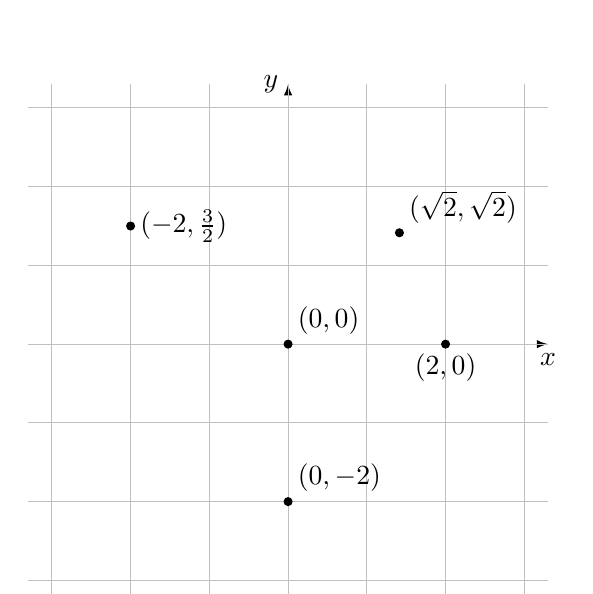
\begin{tikzpicture}
\draw[-latex] (-3.3, 0) -- (3.3, 0) node[below] {$x$} ;
\draw[-latex] (0, -3.3) -- (0, 3.3) node[left] {$y$} ;
\foreach \x in {-3,-2,-1,0,1,2,3} \draw[lightgray] (\x, -3.3) -- (\x, 3.3) ;
\foreach \y in {-3,-2,-1,0,1,2,3} \draw[lightgray] (-3.3, \y) -- (3.3, \y) ;
\draw[fill] (0,0) circle[radius=0.05] node[above right] {$(0,0)$} ;
\draw[fill] ({sqrt(2)},{sqrt(2)}) circle[radius=0.05] node[above right] {$(\sqrt{2},\sqrt{2})$} ;
\draw[fill] (0,-2) circle[radius=0.05] node[above right] {$(0,-2)$} ;
\draw[fill] (2,0) circle[radius=0.05] node[below] {$(2,0)$} ;
\draw[fill] (-2,1.5) circle[radius=0.05] node[right] {$(-2, \frac{3}{2})$} ;
\end{tikzpicture}
\caption{Some points in $\mathbb{R}^2$}
\label{figPointsInR2}
\end{figure}

With this intuition in mind, we set up the following notation.

\begin{notation}
\label{ntnVectorsInRn}
\index{origin}
\index{component}
Let $n \in \mathbb{N}$. Elements of $\mathbb{R}^n$ will be denoted $\vec x, \vec y, \vec z, \dots$\nindex{xvec}{$\vec x$}{vector} \inlatex{vec}\lindexmmc{vec}{$\vec a, \vec b, \dots$} and called ($n$-\textbf{dimensional}) \textbf{vectors}. Given a vector $\vec x \in \mathbb{R}^n$, we write $x_i$ for the $i^{\text{th}}$ \textbf{component} of $\vec x$, so that
\[ \vec x = (x_1,x_2,\dots,x_n) \]
The element $(0,0,\dots,0) \in \mathbb{R}^n$ is called the \textbf{origin} or \textbf{zero vector} of $\mathbb{R}^n$, and is denoted by $\vec 0$.

Moreover, if $\vec x, \vec y \in \mathbb{R}^n$ and $a \in \mathbb{R}$ we write
\[ \vec x + \vec y = (x_1+y_1,x_2+y_2,\dots,x_n+y_n) \quad \text{and} \quad a \vec x = (ax_1,ax_2,\dots,ax_n) \]
\end{notation}

\begin{example}
For all $\vec x \in \mathbb{R}^n$, we have
\[ \vec x + \vec 0 = \vec x \quad \text{and} \quad 1 \vec x = \vec x \]
\end{example}

\begin{definition}
\label{defMagnitude}
\index{magnitude}
\index{distance}
Let $\vec x \in \mathbb{R}^n$. The \textbf{magnitude} of $\vec x$ is the real number $\lVert \vec x \rVert$\nindex{xmag}{$\lVert \vec x \rVert$}{magnitude} \inlatex{lVert\ \textbackslash{}vec\ x\ \textbackslash{}rVert}\lindexmmc{lVert\dots{}\textbackslash{}rVert}{$\lVert \dots{} \rVert$} defined by
\[ \lVert \vec x \rVert = \sqrt{\sum_{i=1}^n x_i^2} = \sqrt{x_1^2+x_2^2+\cdots+x_n^2} \]
Given vectors $\vec x, \vec y \in \mathbb{R}^n$, the \textbf{distance} from $\vec x$ to $\vec y$ is defined to be $\lVert \vec y - \vec x \rVert$. Thus the magnitude of a vector can be thought of as the distance from that vector to the origin.
\end{definition}

\begin{example}
\label{exMagnitudeInR2}
In $\mathbb{R}^2$, \Cref{defMagnitude} says that
\[ \lVert (x,y) \rVert = \sqrt{x^2+y^2} \]
This matches the intuition obtained from the Pythagorean theorem on the sides of right-hand triangles. For example, consider the triangle with vertices $(0,0)$, $(4,0)$ and $(4,3)$:
\begin{center}
\begin{tikzpicture}
\draw (0,0) node [below left] {$(0,0)$}
   -- (4,0) node [below right] {$(4,0)$}
   -- (4,3) node [above right] {$(4,3)$}
   -- (0,0) ;
\end{tikzpicture}
\end{center}
The hypotenuse of the triangle has magnitude
\[ \lVert (4,3) \rVert = \sqrt{4^2+3^2} = \sqrt{25} = 5 \]
\end{example}

\begin{exercise}
\label{exDistanceIsSymmetric}
Let $\vec x, \vec y \in \mathbb{R}^n$. Prove that $\lVert \vec x - \vec y \rVert = \lVert \vec y - \vec x \rVert$. That is, the distance from $\vec x$ to $\vec y$ is equal to the distance from $\vec y$ to $\vec x$.
\end{exercise}

\begin{exercise}
Prove that if $x \in \mathbb{R}$ then the magnitude $\lVert (x) \rVert$ is equal to the absolute value $|x|$.
\end{exercise}

\begin{exercise}
\label{exVectorZeroIffMagnitudeZero}
Let $\vec x \in \mathbb{R}^n$. Prove that $\lVert \vec x \rVert = 0$ if and only if $\vec x = \vec 0$.
\end{exercise}

\subsection*{The triangle inequality and the Cauchy--Schwarz inequality}

The first, and simplest, inequality that we investigate is the (one-dimensional version of the) \textit{triangle inequality} (\Cref{thmTriangleInequality1D}). It is so named because of a generalisation to higher dimensions (\Cref{thmTriangleInequality}), which can be interpreted geometrically as saying that the sum of two side lengths of a triangle is greater than or equal to the third side length.

The triangle inequality is used very frequently in mathematical proofs---you will encounter it repeatedly in this chapter---yet its proof is surprisingly simple.

Before we can prove the triangle inequality, we need the following fact about square roots of real numbers.

\begin{lemma}
\label{lemSquareRootIsOrderPreserving}
Let $x,y \in \mathbb{R}$. If $0 \le x \le y$, then $\sqrt{x} \le \sqrt{y}$.
\end{lemma}
\begin{cproof}
Suppose $0 \le x \le y$. Note that, by definition of the square root symbol, we have $\sqrt{x} \ge 0$ and $\sqrt{y} \ge 0$.

Suppose $\sqrt{x} > \sqrt{y}$. By two applications of \Cref{thmPropertiesOfOrderedFields}(d), we have
\[ y = \sqrt{y} \cdot \sqrt{y} < \sqrt{x} \cdot \sqrt{y} < \sqrt{x} \cdot \sqrt{x} = x \]
so that $y<x$. But this contradicts the assumption that $x \le y$. Hence $\sqrt{x} \le \sqrt{y}$, as required.
\end{cproof}

\begin{theorem}[Triangle inequality in one dimension]
\label{thmTriangleInequality1D}
\index{triangle inequality!in one dimension}
\index{inequality!triangle (one-dimensional)}
Let $x,y \in \mathbb{R}$. Then $|x+y| \le |x|+|y|$. Moreover, $|x+y|=|x|+|y|$ if and only if $x$ and $y$ have the same sign.
\end{theorem}
\begin{cproof}
Note first that $xy \le |xy|$; indeed, $xy$ and $|xy|$ are equal if $xy$ is non-negative, and otherwise we have $xy < 0 < |xy|$. Also $x^2=|x|^2$ and $y^2=|y|^2$. Hence
\[ (x+y)^2 = x^2+2xy+y^2 \le |x|^2+2|xy|+|y|^2 = (|x|+|y|)^2 \]
Taking (nonnegative) square roots yields
\[ |x+y| \le ||x|+|y|| \]
by \Cref{lemSquareRootIsOrderPreserving}. But $|x|+|y| \ge 0$, so $||x|+|y||=|x|+|y|$. This completes the first part of the proof.

Equality holds in the above if and only if $xy=|xy|$, which occurs if and only if $xy \ge 0$. But this is true if and only if $x$ and $y$ are both non-negative or both non-positive---that is, they have the same sign.
\end{cproof}

\begin{example}
Let $x,y \in \mathbb{R}$. We prove that
\[ \frac{|x+y|}{1+|x+y|} \le \frac{|x|}{1+|x|} + \frac{|y|}{1+|y|} \]
First note that, if $0 \le s \le t$, then
\[ \frac{s}{1+s} \le \frac{t}{1+t} \]
To see this, note that
\begin{align*}
s \le t &\Rightarrow 1+s \le 1+t && \text{rearranging} \\
&\Rightarrow \frac{1}{1+t} \le \frac{1}{1+s} && \text{since $1+s,1+t > 0$} \\
&\Rightarrow 1-\frac{1}{1+s} \le 1-\frac{1}{1+t} && \text{rearranging} \\
&\Rightarrow \frac{s}{1+s} \le \frac{t}{1+t} && \text{rearranging}
\end{align*}
Now letting $s=|x+y|$ and $t=|x|+|y|$, we have $s \le t$ by the triangle inequality, and hence
\[ \frac{|x+y|}{1+|x+y|} \le \frac{|x|}{{1+|x|+|y|}} + \frac{|y|}{1+|x|+|y|} \le \frac{|x|}{1+|x|} + \frac{|y|}{1+|y|} \]
as required.
\end{example}

\begin{exercise}
Let $n \in \mathbb{N}$ and let $x_i \in \mathbb{R}$ for each $i \in [n]$. Prove that
\[ \left| \sum_{i=1}^n x_i \right| \le \sum_{i=1}^n |x_i| \]
with equality if and only if the numbers $x_i$ are either all non-positive or all non-negative.
\end{exercise}

\begin{exercise}
Let $x,y \in \mathbb{R}$. Prove that
\[ ||x|-|y|| \le |x-y| \]
\end{exercise}

We will generalise the triangle inequality to arbitrary dimensions in \Cref{thmTriangleInequality}. Our proof will go via the \textit{Cauchy--Schwarz inequality} (\Cref{thmCauchySchwarzInequality}). To motivate the Cauchy--Schwarz inequality, we introduce another geometric notion called the \textit{scalar product} of two vectors.

\begin{definition}
\label{defScalarProduct}
\index{scalar product}
\index{dot product}
Let $\vec x,\vec y \in \mathbb{R}^n$. The \textbf{scalar product} (or \textbf{dot product}) of $\vec x$ with $\vec y$ is the real number $\vec x \cdot \vec y$\nindex{xdoty}{$\vec x \cdot \vec y$}{scalar product} \inlatex{cdot}\lindexmmc{cdot}{$\cdot$} defined by
\[ \vec x \cdot \vec y = \sum_{i=1}^n x_iy_i = x_1y_1+x_2y_2+\cdots+x_ny_n \]
\end{definition}

\begin{example}
\label{exVectorDotItself}
Let $\vec x \in \mathbb{R}^n$. Then $\vec x \cdot \vec x = \lVert \vec x \rVert^2$. Indeed
\[ \vec x \cdot \vec x = \sum_{i=1}^n x_i^2 = \lVert \vec x \rVert^2 \]
\end{example}

\begin{exercise}
\label{exScalarProductIsBilinear}
Let $\vec x, \vec y, \vec z, \vec w \in \mathbb{R}^n$ and let $a,b,c,d \in \mathbb{R}$. Prove that
\[ (a \vec x + b \vec y) \cdot (c \vec z + d \vec w) = ac (\vec x \cdot \vec z) + ad (\vec x \cdot \vec w) + bc( \vec y \cdot \vec z) + bd (\vec y \cdot \vec w) \]
\end{exercise}

Intuitively, the scalar product of two vectors $\vec x$ and $\vec y$ measures the extent to which $\vec x$ and $\vec y$ fail to be \textit{orthogonal}. In fact, if $\theta$ is the acute angle formed between the lines $\ell_1$ and $\ell_2$, where $\ell_1$ passes through $\vec 0$ and $\vec x$ and $\ell_2$ passes through $\vec 0$ and $\vec y$, then a formula for the scalar product of $\vec x$ and $\vec y$ is given by
\[ \vec x \cdot \vec y = \lVert \vec x \rVert \lVert \vec y \rVert \cos \theta \]

\begin{center}
\begin{tikzpicture}[scale=1.5]
\draw [->] (0,0) node [left] {$\vec 0$}
        -- (4,2) node [above right] {$\vec x$} ;
\draw [->] (0,0)
        -- (5,0) node [right] {$\vec y$} ;
\draw [dashed] (4,2) -- (4,0) ;
\draw (3.7,0) -- (3.7,0.3) -- (4,0.3) ;
\draw [<->] (0,-0.3) -- (4,-0.3) ;
\node [below] at (2,-0.3) {$\lVert x \rVert \cos \theta$} ;
\draw [->, domain=0:atan(0.5)] plot ({0.7*cos(\x)},{0.7*sin(\x)}) ;
\node at ({0.85*cos(atan(0.25))}, {0.85*sin(atan(0.25))}) {$\theta$} ;
\end{tikzpicture}
\end{center}

Evidently, $\vec x$ and $\vec y$ are orthogonal if and only if $\cos \theta = 0$, in which case $\vec x \cdot \vec y = 0$ as well. We cannot prove this yet, though, as we have not yet defined trigonometric functions or explored their properties, but hopefully this provides some useful intuition.

The Cauchy--Schwarz inequality provides a useful comparison of the size of a scalar product of two vectors with the magnitudes of the vectors.

\begin{theorem}[Cauchy--Schwarz inequality]
\label{thmCauchySchwarzInequality}
\index{Cauchy--Schwarz inequality}
\index{inequality!Cauchy--Schwarz}
Let $n \in \mathbb{N}$ and let $x_i,y_i \in \mathbb{R}$ for each $i \in [n]$. Then
\[ |\vec x \cdot \vec y| \le \lVert \vec x \rVert \lVert \vec y \rVert \]
with equality if and only if $a\vec x = b\vec y$ for some $a,b \in \mathbb{R}$ which are not both zero.
\end{theorem}
\begin{cproof}
If $\vec y = \vec 0$, then this is trivial: both sides of the equation are equal to zero! So assume that $\vec y \ne \vec 0$. In particular, by \Cref{exVectorZeroIffMagnitudeZero}, we have $\lVert \vec y \rVert > 0$.

Define $k = \dfrac{\vec x \cdot \vec y}{\lVert \vec y \rVert^2}$. Then
\begin{align*}
0 &\le \lVert \vec x - k \vec y \rVert^2 && \text{since squares are nonnegative} \\
&= (\vec x - k \vec y) \cdot (\vec x - k \vec y) && \text{by \Cref{exVectorDotItself}} \\
&= (\vec x \cdot \vec x) - 2k (\vec x \cdot \vec y) + k^2 (\vec y \cdot \vec y) && \text{by \Cref{exScalarProductIsBilinear}} \\
&= \lVert \vec x \rVert^2 - \frac{(\vec x \cdot \vec y)^2}{\lVert y \rVert^2} && \text{by definition of $k$}
\end{align*}
Multiplying through by $\lVert \vec y \rVert^2$, which is non-negative and therefore doesn't change the sign of the inequality, yields
\[ 0 \le \lVert \vec x \rVert^2 \lVert \vec y \rVert^2 - (\vec x \cdot \vec y)^2 \]
which is equivalent to what was to be proved.

Evidently, equality holds if and only if $\lVert \vec x - k \vec y \rVert = 0$, which by \Cref{exVectorZeroIffMagnitudeZero} occurs if and only if $\vec x - k \vec y = 0$. Now:
\begin{itemize}
\item If $\vec x - k\vec y = 0$, then we have
\begin{align*}
&\vec x - k \vec y = 0 && \\
&\Leftrightarrow \vec x - \frac{\vec x \cdot \vec y}{\lVert \vec y \rVert^2} \vec y = 0 && \text{by definition of $k$} \\
&\Leftrightarrow \lVert \vec y \rVert^2 \vec x = (\vec x \cdot \vec y) \vec y && \text{rearranging}
\end{align*}
If $\vec y \ne \vec 0$ then let $a=\lVert \vec y \rVert^2$ and $b=\vec x \cdot \vec y$; otherwise, let $a=0$ and $b=1$. In both cases, we have $a \vec x = b \vec y$ and $a,b$ are not both zero.

If $a \vec x = b \vec y$ for some $a,b \in \mathbb{R}$ not both zero, then either:
\begin{itemize}
\item $a=0$ and $b \ne 0$, in which case $\vec y = 0$ and we have equality in the Cauchy--Schwarz inequality; or
\item $a \ne 0$, in which case $\vec y = \frac{b}{a} \vec x$. Write $c=\frac{b}{a}$. Then
\begin{align*}
|\vec x \cdot \vec y| &= | \vec x \cdot (c \vec x) | && \\
&= |c(\vec x \cdot \vec x)| && \text{by \Cref{exScalarProductIsBilinear}} \\
&= |c| \lVert \vec x \rVert^2 && \text{by \Cref{exVectorDotItself}} \\
&= \lVert \vec x \rVert \lVert c \vec x \rVert && \text{rearranging} \\
&= \lVert \vec x \rVert \lVert \vec y \rVert &&
\end{align*}
\end{itemize}
In either case, we have equality in the Cauchy--Schwarz inequality.
\end{itemize}

So equality holds if and only if $a \vec x = b \vec y$ for some $a,b \in \mathbb{R}$ not both zero.
\end{cproof}

\begin{example}
Let $a,b,c \in \mathbb{R}$. We'll prove that
\[ ab+bc+ca \le a^2+b^2+c^2 \]
and examine when equality holds.

Letting $\vec x = (a,b,c)$ and $\vec y = (b,c,a)$ yields
\[ \vec x \cdot \vec y = ab+bc+ca \]
and
\[ \lVert \vec x \rVert = \sqrt{a^2+b^2+c^2} = \sqrt{b^2+c^2+a^2} = \lVert \vec y \rVert \]
Hence $\lVert \vec x \rVert \lVert \vec y \rVert = a^2+b^2+c^2$. By the Cauchy--Schwarz inequality, it follows that
\[ \vec x \cdot \vec y = ab+bc+ca \le a^2+b^2+c^2 = \lVert \vec x \rVert \lVert \vec y \rVert \]
as required. Equality holds if and only if $k(a,b,c) = \ell(b,c,a)$ for some $k,\ell \in \mathbb{R}$ not both zero. We may assume $k \ne 0$---otherwise, swap the vectors $\vec x$ and $\vec y$ in what follows. Then, letting $t=\frac{\ell}{k}$, we have
\begin{align*}
&k(a,b,c) = \ell(b,c,a) && \\
&\Leftrightarrow (a,b,c) = (tb,tc,ta) && \text{by definition of $t$} \\
&\Leftrightarrow (a,b,c) = (t^2c,t^2a,t^2b) && \text{substituting $a=tb$ etc.} \\
&\Leftrightarrow (a,b,c) = (t^3a,t^3b,t^3c) && \text{substituting $a=tb$ etc.\ again} \\
&\Leftrightarrow \vec x = t^3 \vec x
\end{align*}
This occurs if and only if either $(a,b,c)=(0,0,0)$, or $t=1$, in which case
\[ (a,b,c) = (tb,tc,ta) = (b,c,a) \]
So equality holds if and only if $a=b=c$.
\end{example}

\begin{exercise}
Let $r \in \mathbb{N}$ and let $a_1,a_2,\dots,a_r \in \mathbb{R}$ be such that $a_1^2+a_2^2+\cdots+a_n^2=6$. Prove that
\[ (a_1+2a_2+\cdots+na_n)^2 \le n(n+1)(2n+1) \]
and determine when equality holds.
\end{exercise}

We now use the Cauchy--Schwarz inequality to generalise the one-dimensional version of the triangle inequality (\Cref{thmTriangleInequality1D}) to arbitrary (finite) dimensions.

\begin{theorem}[Triangle inequality]
\label{thmTriangleInequality}
\index{triangle inequality}
\index{inequality!triangle}
Let $\vec x, \vec y \in \mathbb{R}^n$. Then
\[ \lVert \vec x + \vec y \rVert \le \lVert \vec x \rVert + \lVert \vec y \rVert \]
with equality if and only if $a\vec x = b\vec y$ for some real numbers $a,b \ge 0$.
\end{theorem}

\begin{cproof}
We proceed by calculation:
\begin{align*}
\lVert \vec x + \vec y \rVert^2
&= (\vec x + \vec y) \cdot (\vec x + \vec y) && \text{by \Cref{exVectorDotItself}} \\
&= (\vec x \cdot \vec x) + 2(\vec x \cdot \vec y) + (\vec y \cdot \vec y) && \text{by \Cref{exScalarProductIsBilinear}} \\
&\le (\vec x \cdot \vec x) + 2|\vec x \cdot \vec y| + (\vec y \cdot \vec y) && \text{since $a \le |a|$ for all $a \in \mathbb{R}$} \\
&\le \lVert \vec x \rVert^2 + 2\lVert x \rVert \lVert y \rVert + \lVert \vec y \rVert^2 && \text{by \Cref{exVectorDotItself} and Cauchy--Schwarz} \\
&= (\lVert \vec x \rVert + \lVert \vec y \rVert)^2 && \text{rearranging}
\end{align*}

Taking (nonnegative) square roots of both sides yields
\[ \lVert \vec x + \vec y \rVert \le \lVert \vec x \rVert + \lVert \vec y \rVert \]
by \Cref{lemSquareRootIsOrderPreserving}, as required.

Equality holds if and only if the two `$\le$' symbols in the above derivation are in fact `$=$' symbols.
\begin{itemize}
\item The first inequality is equality if and only if $\vec x \cdot \vec y = |\vec x \cdot \vec y|$, which holds if and only if $\vec x \cdot \vec y \ge 0$.
\item The second inequality is equality if and only if equality holds in the Cauchy--Schwarz inequality. In turn, this occurs if and only if $a\vec x = b \vec y$ for some $a,b \in \mathbb{R}$. We may, moreover, assume that $a \ge 0$---if not, replace $a$ and $b$ by their negatives.
\end{itemize}
If $a=0$ then we can take $b=0$.
%% BEGIN EXTRACT {xtrSoExampleTwo} %%
If $a>0$, then by \Cref{exVectorDotItself} and \Cref{exScalarProductIsBilinear}, we have
\[ \vec x \cdot \left( \frac{b}{a} \vec x \right) = \frac{b}{a} \lVert \vec x \rVert^2 \]
which is non-negative if and only if $b \ge 0$, since we are assuming that $a \ge 0$.
%% END EXTRACT %%

Thus, equality holds in the triangle inequality if and only if $a\vec x = b\vec y$ for some $a,b \ge 0$.
\end{cproof}

This general version of the triangle inequality has a geometric interpretation in terms of---you guessed it---triangles. Any three points $\vec a, \vec b, \vec c \in \mathbb{R}^n$ form a (potentially flat) triangle:

\begin{center}
\begin{tikzpicture}
\draw (0,2) -- (7,0) node[pos=0, left] {$\vec a$}
                     node[midway, below left] {$u$}
            -- (3,4) node[pos=0, right] {$\vec b$}
                     node[midway, above right] {$v$}
            -- (0,2) node[pos=0, above] {$\vec c$}
                     node[midway, above left] {$w$};
\end{tikzpicture}
\end{center}

The side lengths $u,v,w$ are given by the following equations:
\[ u = \lVert \vec b - \vec a \rVert, \quad v = \lVert \vec c - \vec b \rVert, \quad w = \lVert \vec a - \vec c \rVert \]
The triangle inequality says tells us that $u \le v + w$. Indeed:
\begin{align*}
u &= \lVert \vec b - \vec a \rVert && \text{by definition of $u$} \\
&= \lVert (\vec b - \vec c) + (\vec c - \vec a) \rVert && \text{rearranging} \\
&\le \lVert \vec b - \vec c \rVert + \lVert \vec c - \vec a \rVert && \text{by the triangle inequality} \\
&= \lVert \vec c - \vec b \rVert + \lVert \vec a - \vec c \rVert && \text{by \Cref{exDistanceIsSymmetric}} \\
&= v + w && \text{by definition of $v$ and $w$}
\end{align*}

That is, the triangle inequality says that the sum of two side lengths of a triangle is greater than or equal to the third side length. Moreover, it tells us $u=v+w$ precisely when $k(\vec a - \vec c) = \ell(\vec c - \vec b)$ for some $k,\ell \ge 0$. If $k=0$ then
\[ \vec c \quad = \quad \vec b \quad = \quad 0 \vec a + (1-0) \vec b \]
if $k>0$, then $k+\ell>0$, so we have
\[ \vec c \quad = \quad \frac{k}{k+\ell} \vec a + \frac{\ell}{k+\ell} \vec b \quad = \quad \frac{k}{k+\ell} \vec a + \left( 1 - \frac{k}{k+\ell} \right)\vec b \]
Examining this a bit more closely yields that $u=v+w$ if and only if
\[ \vec c = t\vec a + (1-t) \vec b \]
for some $0 \le t \le 1$, which is to say precisely that $\vec c$ lies on the line segment between $\vec a$ and $\vec b$. In other words, equality holds in the triangle inequality only if the three vertices of the triangle are \textit{collinear}, which is to say that the triangle whose vertices are the points $\vec a$, $\vec b$ and $\vec c$, is flat.

\subsection*{Inequalities of means}

Our goal now is to explore different kinds of average---specifically, \textit{means}---of finite sets of non-negative real numbers. We will compare the relative sizes of these means with respect to one-another, with emphasis on three particular kinds of mean: the \textit{arithmetic mean} (\Cref{defArithmeticMean}), the \textit{geometric mean} (\Cref{defGeometricMean}) and the \textit{harmonic mean} (\Cref{defHarmonicMean}). These means in fact assemble into a continuum of means, called \textit{generalised means} (\Cref{defGeneralisedMean}), all of which can be compared with one another.

\begin{definition}
\label{defArithmeticMean}
\index{mean!arithmetic}
Let $n \ge 1$. The (\textbf{arithmetic}) \textbf{mean} of real numbers $x_1,\dots,x_n$ is
\[ \frac{1}{n} \sum_{i=1}^n x_i = \frac{x_1 + x_2 + \cdots + x_n}{n} \]
\end{definition}

\begin{definition}
\label{defGeometricMean}
\index{mean!geometric}
Let $n \ge 1$. The \textbf{geometric mean} of non-negative real numbers $x_1,\dots,x_n$ is
\[ \sqrt[n]{\prod_{i=1}^n x_i} = \sqrt[n]{x_1 \cdot x_2 \cdot \dots \cdot x_n} \]
\end{definition}

The following theorem is commonly known as the \textbf{AM--GM inequality}.

\begin{theorem}[Inequality of arithmetic and geometric means]
\label{thmAMGMInequality}
\index{AM--GM inequality}
\index{inequality!of arithmetic and harmonic means}
Let $n \in \mathbb{N}$ and $x_1,x_2,\dots,x_n \ge 0$. Then
\[ \underbrace{\sqrt[n]{x_1 \cdots x_n}}_{\text{geometric mean}} \le \underbrace{\frac{x_1 + \cdots + x_n}{n}}_{\text{arithmetic mean}} \]
with equality if and only if $x_1 = \cdots = x_n$.
\end{theorem}
\begin{cproof}[when $n=2$]
We need to show that, if $x,y \in \mathbb{R}$ with $x, y \ge 0$, then
\[ \sqrt{xy} \le \frac{x+y}{2} \]
with equality if and only if $x=y$.

First note that the square roots of $x$ and $y$ exist since they are non-negative. Now
\begin{align*}
0 &\le (\sqrt{x}-\sqrt{y})^2 && \text{since squares are nonnegative} \\
&= (\sqrt{x})^2 - 2\sqrt{x}\sqrt{y} + (\sqrt{y})^2 && \text{expanding} \\
&= x - 2\sqrt{xy} + y && \text{rearranging}
\end{align*}

Rearranging the inequality $0 \le x-2\sqrt{xy}+y$ yields the desired result.

If $\sqrt{xy} = \frac{x+y}{2}$, then we can rearrange the equation as follows:
\begin{align*}
\sqrt{xy} = \frac{x+y}{2} &\Rightarrow 2\sqrt{xy} = x+y && \text{multiplying by $2$} \\
&\Rightarrow 4xy = x^2+2xy+y^2 && \text{squaring both sides} \\
&\Rightarrow x^2-2xy+y^2 = 0 && \text{rearranging} \\
&\Rightarrow (x-y)^2 = 0 && \text{factorising} \\
&\Rightarrow x-y = 0 && \text{since $a^2=0 \Rightarrow a=0$ for $a \in \mathbb{R}$} \\
&\Rightarrow x=y && \text{rearranging}
\end{align*}
So we have proved both parts of the theorem.
\end{cproof}

\begin{example}
We use the AM--GM inequality to prove that the area of a rectangle with fixed perimeter is maximised when the rectangle is a square.

Indeed, fix a perimeter $p > 0$, and let $x,y > 0$ be side lengths of a rectangle with perimeter $p$---that is, $x$ and $y$ satisfy the equation $2x+2y=p$. The area $a$ of the rectangle satisfies $a=xy$. By the AM--GM inequality, we have
\[ a = xy \le \left( \frac{x+y}{2} \right)^2 = \frac{p^2}{16} \]
Equality holds if and only if $x=y$, in other words, if and only if the rectangle is a square.
\end{example}

\begin{exercise}
Let $a,b > 0$ be real numbers. Prove that $\displaystyle \frac{a^2+b^2}{2} \ge ab$.
\end{exercise}

\begin{example}
Let $x>0$. We find the minimum possible value of $x+\frac{9}{x}$. By the AM--GM inequality, we have
\[ x+\frac{9}{x} \ge 2\sqrt{x \cdot \frac{9}{x}} = 2 \sqrt{9} = 6 \]
with equality if and only if $x=\frac{9}{x}$, which occurs if and only if $x=3$. Hence the minimum value of $x+\frac{9}{x}$ when $x>0$ is $6$.
\end{example}

\begin{exercise}
Let $x>0$ and let $n \in \mathbb{N}$. Find the minimum possible value of $\displaystyle \sum_{k=-n}^n x^k$.
\end{exercise}

\Cref{exAMGMForPowersOf2,exAMGMForPredecessors} complete the proof of the AM--GM inequality (\Cref{thmAMGMInequality}). Before proceeding with the exercises, let's fix some notation: for each $n \in \mathbb{N}$, let $p_{\text{AM--GM}}(n)$ be the assertion that
the AM--GM inequality holds for collections of $n$ numbers; that is, $p_{\text{AM--GM}}(n)$ is the assertion:
\begin{quote}
For all $x_1,x_2,\dots,x_n \ge 0$, we have
\[ \sqrt[n]{\prod_{i=1}^n x_i} \le \frac{1}{n} \sum_{i=1}^n x_i \]
with equality if and only if $x_1=x_2=\cdots=x_n$.
\end{quote}
Note that we already proved $p_{\text{AM--GM}}(2)$.

\begin{exercise}
\label{exAMGMForPowersOf2}
Let $r \in \mathbb{N}$ and let $x_1,x_2,\dots,x_{2r} \in \mathbb{R}$. Write
\[ a = \frac{1}{r} \sum_{i=1}^r x_i \quad \text{and} \quad g = \sqrt[r]{\prod_{i=1}^r x_i} \]
for the arithmetic and geometric means, respectively, of the numbers $x_1,\dots,x_r$; write
\[ a' = \frac{1}{r} \sum_{i=r+1}^{2r} x_i \quad \text{and} \quad g' = \sqrt[r]{\prod_{i=r+1}^{2r} x_i} \]
for the arithmetic and geometric means, respectively, of the numbers $x_{r+1},\dots,x_{2r}$; and write
\[ A = \frac{1}{2r} \sum_{i=1}^{2r} x_i \quad \text{and} \quad G = \sqrt[2r]{\prod_{i=1}^{2r} x_i} \]
for the arithmetic and geometric means, respectively, of all the numbers $x_1,\dots,x_{2r}$.

Prove that
\[ A = \frac{a+a'}{2} \quad \text{and} \quad G=\sqrt{gg'} \]
Deduce that, for each $r \in \mathbb{N}$, if $p_{\text{AM--GM}}(r)$ is true then $p_{\text{AM--GM}}(2r)$ is true. Deduce further than $p_{\text{AM--GM}}(2^m)$ is true for all $m \in \mathbb{N}$.
\end{exercise}

\begin{exercise}
\label{exAMGMForPredecessors}
Let $r \ge 2$ and let $x_1,\dots,x_{r-1} \in \mathbb{N}$. Define
\[ x_r = \frac{1}{r-1} \sum_{i=1}^{r-1} x_i \]
Prove that
\[ \frac{1}{r}\sum_{i=1}^r x_i = x_r \]
Assuming $p_{\text{AM--GM}}(r)$, deduce that
\[ x_r^r \ge \prod_{i=1}^r x_i = \left(\prod_{i=1}^{r-1} x_i\right) \cdot x_r \]
with equality if and only if $x_1=x_2=\cdots=x_r$. Deduce that $p_{\text{AM--GM}}(r)$ implies $p_{\text{AM--GM}}(r-1)$. Use \Cref{exAMGMForPowersOf2} to deduce further that $p_{\text{AM--GM}}(n)$ is true for all $n \ge 1$.
\end{exercise}

We now introduce another kind of mean, called the \textit{harmonic mean}.

\begin{definition}
\label{defHarmonicMean}
\index{mean!harmonic}
Let $n \in \mathbb{N}$. The \textbf{harmonic mean} of nonzero real numbers $x_1,x_2,\dots,x_n$ is
\[ \left( \frac{1}{n} \sum_{i=1}^n x_i^{-1} \right)^{-1} = \cfrac{n}{\frac{1}{x_1} + \frac{1}{x_2} + \cdots + \frac{1}{x_n}} \]
\end{definition}

The harmonic mean of two nonzero real numbers $x$ and $y$ has a simpler expression:
\[ \left( \frac{x^{-1}+y^{-1}}{2} \right)^{-1} = \frac{2xy}{x+y} \]

The harmonic mean arises naturally when considering rates of change of quantities over fixed amounts of time.

\begin{example}
The cities of York and Leeds are located $d>0$ miles apart. Two cars drive from York to Leeds, then immediately turn around and drive back. The two cars depart from York at the same time and arrive back in York at the same time.
\begin{itemize}
\item The first car drives from York to Leeds at a constant speed of $u$ miles per hour, and drives back to York at a constant speed of $v$ miles per hour.
\item The second car drives from York to Leeds and back again at the same constant speed of $w$ miles per hour.
\end{itemize}
According to the following formula from physics:
\[ \text{speed} \times \text{time} = \text{distance} \]
the time spent driving by the first car is $\frac{d}{u} + \frac{d}{v}$, and the time spent driving by the second car is $\frac{2d}{w}$.

Since the cars spend the same amount of time driving, it follows that
\[ \frac{2d}{w} = \frac{d}{u} + \frac{d}{v} \qquad \Rightarrow \qquad w = \frac{2uv}{u+v} \]
That is, the second car's speed is the harmonic mean of the two speeds driven by the first car.
\end{example}

As might be expected, we now prove a theorem relating the harmonic means with the other means we have established so far---this theorem is known as the \textbf{GM--HM inequality}.

\begin{theorem}[Inequality of geometric and harmonic means]
\label{thmGMHMInequality}
\index{GM--HM inequality}
\index{inequality!of geometric and harmonic means}
Let $n \in \mathbb{N}$ and $x_1,x_2,\dots,x_n > 0$. Then
\[ \underbrace{\cfrac{n}{\frac{1}{x_1} + \frac{1}{x_2} + \cdots + \frac{1}{x_n}}}_{\text{harmonic mean}} \le \underbrace{\sqrt[n]{x_1x_2 \cdots x_n}}_{\text{geometric mean}} \]
with equality if and only if $x_1 = \cdots = x_n$.
\end{theorem}
\begin{cproof}[when $n=2$]
We need to prove that if $x,y > 0$, then
\[ \frac{2}{\frac{1}{x} + \frac{1}{y}} \le \sqrt{xy} \]
This is almost immediate from the AM--GM inequality (\Cref{thmAMGMInequality}). Indeed, since all numbers in sight are positive, we can take reciprocals to see that this inequality is equivalent to the assertion that
\[ \frac{1}{\sqrt{xy}} \le \frac{x^{-1} + y^{-1}}{2} \]
But $\frac{1}{\sqrt{xy}} = \sqrt{x^{-1}y^{-1}}$, so this is immediate from the AM--GM inequality.
\end{cproof}

\begin{exercise}
Prove the GM--HM inequality for general values of $n \in \mathbb{N}$.
\end{exercise}

Another example of a mean that has applications in probability theory and statistics is that of the \textit{quadratic mean}.

\begin{definition}
\label{defQuadraticMean}
\index{mean!quadratic}
\index{root-mean-square}
Let $n \in \mathbb{N}$. The \textbf{quadratic mean} (or \textbf{root-mean-square}) of real numbers $x_1,x_2,\dots,x_n$ is
\[ \left( \frac{1}{n} \sum_{i=1}^n x_i^2 \right)^{\frac{1}{2}} = \sqrt{\frac{x_1^2+x_2^2+\cdots+x_n^2}{n}} \]
\end{definition}

The following theorem is, predictably, known as the \textbf{QM--AM inequality} (or \textbf{RMS--AM inequality}); it is a nice application of the Cauchy--Schwarz inequality.

\begin{theorem}[Inequality of quadratic and arithmetic means]
\label{thmQMAMInequality}
\index{QM--AM inequality}
\index{inequality!of quadratic and arithmetic means}
Let $n > 0$ and $x_1,x_2,\dots,x_n \ge 0$. Then
\[ \underbrace{\frac{x_1 + \cdots + x_n}{n}}_{\text{arithmetic mean}} \le \underbrace{\sqrt{\frac{x_1^2+x_2^2+\cdots+x_n^2}{n}}}_{\text{quadratic mean}} \]
with equality if and only if $x_1 = \cdots = x_n$.
\end{theorem}

\begin{cproof}
Define
\[ \vec x = (x_1,x_2,\dots,x_n) \quad \text{and} \quad \vec y = (1,1,\dots,1) \]
Then
\begin{align*}
x_1+x_2+\cdots+x_n
&= \vec x \cdot \vec y && \text{by definition of scalar product} \\
&\le \lVert \vec x \rVert \lVert \vec y \rVert && \text{by Cauchy--Schwarz} \\
&= \sqrt{x_1^2+x_2^2+\cdots+x_n^2} \cdot \sqrt{n} && \text{evaluating the magnitudes}
\end{align*}
Dividing through by $n$ yields
\[ \frac{x_1+x_2+\cdots+x_n}{n} \le \sqrt{\frac{x_1^2+x_2^2+\cdots+x_n^2}{n}} \]
as required. Equality holds if and only if equality holds in the Cauchy--Schwarz inequality, which occurs if and only if
\[ (ax_1,ax_2,\dots,ax_n)=(b,b,\dots,b) \]
for some $a,b \in \mathbb{R}$ not both zero. If $a=0$ then $b=0$, so we must have $a \ne 0$. Hence equality holds if and only if $x_i=\frac{b}{a}$ for all $i \in [n]$---in particular, if and only if $x_1=x_2=\cdots=x_n$.
\end{cproof}

To summarise, what we have proved so far is
\[ \begin{matrix} \text{harmonic} \\ \text{mean} \end{matrix} \quad \overset{(\ref{thmGMHMInequality})}{\le} \quad \begin{matrix} \text{geometric} \\ \text{mean} \end{matrix} \quad \overset{(\ref{thmAMGMInequality})}{\le} \quad \begin{matrix} \text{arithmetic} \\ \text{mean} \end{matrix} \quad \overset{(\ref{thmQMAMInequality})}{\le} \quad \begin{matrix} \text{quadratic} \\ \text{mean} \end{matrix} \]
with equality in each case if and only if the real numbers whose means we are taking are all equal.

The following exercise allows us to bookend our chain of inequalities with the minimum and maximum of the collections of numbers.

\begin{exercise}
\label{exMinMeanMaxInequalities}
Let $n > 0$ and let $x_1,x_2,\dots,x_n$ be positive real numbers. Prove that
\[ \mathrm{min} \{ x_1,x_2,\dots,x_n \} \le \left( \frac{1}{n} \sum_{i=1}^n x_i^{-1} \right)^{-1} \quad \text{and} \quad \mathrm{max} \{ x_1,x_2,\dots,x_n \} \ge \left( \frac{1}{n} \sum_{i=1}^n x_i^2 \right)^{\frac{1}{2}} \]
with equality in each case if and only if $x_1=x_2=\cdots=x_n$.
\end{exercise}

\subsection*{\optmark{Generalised means}}

We conclude this section by mentioning a generalisation of the results we have proved about means. We are not yet ready to prove the results that we mention; they are only here for the sake of interest.

\begin{definition}
\label{defExtendedRealLine}
\index{extended real number line}
The \textbf{extended real number line} is the (ordered) set $[-\infty, \infty]$, defined by
\[ [-\infty,\infty] = \mathbb{R} \cup \{ -\infty, \infty \} \]
where $\mathbb{R}$ is the set of real numbers with its usual ordering, and $-\infty,\infty$ are new elements ordered in such a way that $-\infty < x < \infty$ for all $x \in \mathbb{R}$.
\end{definition}

Note that the extended real line does \textit{not} form a field---the arithmetic operations are not defined on $-\infty$ or $\infty$, and we will at no point treat $-\infty$ and $\infty$ as real numbers; they are merely elements which extend the reals to add a least element and a greatest element.

\begin{definition}
\label{defGeneralisedMean}
\index{mean!generalised}
Let $p \in [-\infty,\infty]$, let $n \in \mathbb{N}$, and let $x_1,x_2,\dots,x_n$ be positive real numbers. The \textbf{generalised mean with exponent $p$} (or simply $p$-\textbf{mean}) $x_1,x_2,\dots,x_n$ is the real number $M_p(x_1,x_2,\dots,x_n)$ defined by
\[ M_p(x_1,x_2,\dots,x_n) = \left( \frac{1}{n} \sum_{i=1}^n x_i^p \right)^{\frac{1}{p}} \]
if $p \not \in \{ -\infty, 0, \infty \}$, and by
\[ M_p(x_1,x_2,\dots,x_n) = \lim_{q \to p} M_q(x_1,x_2,\dots,x_n) \]
if $p \in \{ -\infty, 0, \infty \}$, where the notation $\lim\limits_{q \to p}$ refers to the \textit{limit} as $q$ tends to $p$, as discussed in \Cref{secLimitsOfFunctions}.
\end{definition}

We can see immediately that the harmonic, arithmetic and quadratic means of a finite set of positive real numbers are the $p$-means for a suitable value of $p$: the harmonic mean is the $(-1)$-mean, the arithmetic mean is the $1$-mean, and the quadratic mean is the $2$-mean. Furthermore, \Cref{propZeroAndInfinityMeans} exhibits the \textit{minimum} as the $(-\infty)$-mean, the \textit{geometric mean} as the $0$-mean, and the \textit{maximum} as the $\infty$-mean.

\begin{proposition}
\label{propZeroAndInfinityMeans}
Let $n > 0$ and let $x_1,x_2,\dots,x_n \ge 0$. Then
\begin{itemize}
\item $M_{-\infty}(x_1,x_2,\dots,x_n) = \mathrm{min}\{ x_1,x_2,\dots,x_n \}$;
\item $M_0(x_1,x_2,\dots,x_n) = \sqrt[n]{x_1x_2\cdots x_n}$; and
\item $M_{\infty}(x_1,x_2,\dots,x_n) = \mathrm{min}\{ x_1,x_2,\dots,x_n \}$. \qed
\end{itemize}
\end{proposition}

All of the inequalities of means we have seen so far will be subsumed by \Cref{thmGeneralisedMeanInequality}, which compares the $p$-mean and $q$-mean of a set of numbers for all values of $p,q \in [-\infty,\infty]$.

\begin{theorem}
\label{thmGeneralisedMeanInequality}
\index{inequality!of generalised means}
Let $n > 0$, let $x_1,x_2,\dots,x_n \ge 0$ and let $p,q \in [-\infty,\infty]$ with $p<q$. Then
\[ M_p(x_1,x_2,\dots,x_n) \le M_q(x_1,x_2,\dots,x_n) \]
with equality if and only if $x_1=x_2=\cdots=x_n$. \qed
\end{theorem}

\Cref{thmGeneralisedMeanInequality} implies each of the following:
\begin{itemize}
\item \textbf{HM--min inequality} (\Cref{exMinMeanMaxInequalities}): take $p=-\infty$ and $q=-1$;
\item \textbf{GM--HM inequality} (\Cref{thmGMHMInequality}): take $p=-1$ and $q=0$;
\item \textbf{AM--GM inequality} (\Cref{thmAMGMInequality}): take $p=0$ and $q=1$;
\item \textbf{QM--AM inequality} (\Cref{thmQMAMInequality}): take $p=1$ and $q=2$;
\item \textbf{max--QM inequality} (\Cref{exMinMeanMaxInequalities}): take $p=2$ and $q=\infty$.
\end{itemize}

\newpage
% !TeX root = ../../book.tex
\section{Completeness and convergence}
\secbegin{secCompletenessConvergence}

For most of the results that we proved in \Cref{secInequalitiesMeans}, it did not matter that we were talking about real numbers. We could just as well have been working with any other ordered field, such as the rational numbers---that is, most of the results in \Cref{secInequalitiesMeans} remain true by replacing $\mathbb{R}$ by $\mathbb{Q}$ (or any other ordered field) throughout.

From here onwards, we isolate the property of $\mathbb{R}$ that separates it from $\mathbb{Q}$---namely, \textit{completeness}. It is completeness that will allow us to define and explore the fundamental concepts of mathematical analysis: sequences, functions, convergence, limits, continuity, differentiability, and so on.

The property of completeness concerns least upper bounds for certain sets of real numbers.

\begin{definition}
\label{defSupremumOfSubsetOfR}
\index{upper bound!of subset of $\mathbb{R}$}
\index{supremum!of subset of $\mathbb{R}$}
Let $A \subseteq \mathbb{R}$. A real number $m$ is an \textbf{upper bound} for $A$ if $a \le m$ for all $a \in A$. A \textbf{supremum} of $A$ is a \textit{least} upper bound of $A$; that is, a real number $m$ such that:
\begin{enumerate}[(i)]
\item $m$ is an upper bound of $A$---that is, $a \le m$ for all $a \in A$; and
\item $m$ is least amongst all upper bounds for $A$---that is, for all $x \in \mathbb{R}$, if $a \le x$ for all $a \in A$, then $x \le m$.
\end{enumerate}
\end{definition}

\begin{example}
We prove that $1$ is a supremum of the open interval $(0,1)$.
\begin{enumerate}[(i)]
\item Let $a \in (0,1)$. Then $a < 1$, so that $1$ is an upper bound of $(0,1)$.
\item Let $x \in \mathbb{R}$ be another upper bound of $(0,1)$. If $x < 1$, then we have
\[ x = \dfrac{x+x}{2} < \dfrac{x+1}{2} < \dfrac{1+1}{2} = 1 \]
and so $x < \dfrac{x+1}{2} \in (0,1)$. This contradicts the assumption that $x$ is an upper bound of $(0,1)$. It follows that $x \ge 1$, as required.
\end{enumerate}
Hence $1$ is indeed a supremum of $(0,1)$.
\end{example}

\begin{exercise}
\label{exDefineLowerBoundInfimum}
\index{lower bound!of subset of $\mathbb{R}$}
\index{infimum!of subset of $\mathbb{R}$}
Define the notions of \textbf{lower bound} and \textbf{infimum}, and find the infimum of the open interval $(0,1)$.
\end{exercise}

The following proposition provides a convenient way of testing whether a real number is a supremum of a subset.

\begin{proposition}
\label{propSupremumEpsilon}
Let $A \subseteq \mathbb{R}$ and suppose $m \in \mathbb{R}$ is an upper bound of $A$. Then $m$ is a supremum of $A$ if and only if, for all $\varepsilon > 0$, there exists $a \in A$ such that $a > m-\varepsilon$.
\end{proposition}

\begin{cproof}
\fixlistskip
\begin{itemize}
\item ($\Rightarrow$). Suppose $m$ is a supremum of $A$, and let $\varepsilon > 0$. If there is no $a \in A$ such that $a > m - \varepsilon$, then $a \le m-\varepsilon$ for all $a \in A$. But this contradicts the assumption that $m$ is a supremum of $a$, since $m-\varepsilon$ is an upper bound of $A$ that is less than $m$. So there exists $a \in A$ with $a > m - \varepsilon$, as required.

\item ($\Leftarrow$). Suppose that, for all $\varepsilon > 0$, there exists $a \in A$ with $a > m-\varepsilon$, and let $x \in \mathbb{R}$ be an upper bound of $A$. In order to prove that $m$ is a supremum of $A$, we must prove that $m \le x$.

Suppose $x < m$, and define $\varepsilon = m-x$. Then $\varepsilon > 0$, so there exists $a \in A$ such that
\[ a > m - \varepsilon = m - (m-x) = x \]
But this contradicts the assumption that $x$ is an upper bound of $A$. So we must have $m \le x$, as required.
\end{itemize}
\end{cproof}

\begin{theorem}[Uniqueness of suprema]
Let $A$ be a subset of $\mathbb{R}$. If $m_1$ and $m_2$ are suprema of $A$, then $m_1 = m_2$.
\end{theorem}

\begin{cproof}
Since $m_1$ is an upper bound of $A$ and $m_2$ is a supremum of $A$, we have $m_2 \ge m_1$ by \Cref{defSupremumOfSubsetOfR}(ii). Likewise, since $m_2$ is an upper bound of $A$ and $m_1$ is a supremum of $A$, we have $m_1 \ge m_2$ by \Cref{defSupremumOfSubsetOfR}(ii) again. But this implies that $m_1 = m_2$.
\end{cproof}

An analogous result proves that a subset of $\mathbb{R}$ may have at most one infimum. This allows us to introduce the following notation.

\begin{definition}
\nindex{supremum}{$\mathrm{sup}(A)$}{supremum}
\nindex{infimum}{$\mathrm{inf}(A)$}{infimum}
Let $A \subseteq \mathbb{R}$. The supremum of $A$, if it exists is denoted by $\mathrm{sup}(A)$ \inlatex{mathrm\{sup\}}\lindexmmc{mathrm}{$\mathrm{Aa}, \mathrm{Bb}, \dots$}; the infimum of $A$, if it exists, is denoted by $\mathrm{inf}(A)$ \inlatex{mathrm\{inf\}}.
\end{definition}

Now that we are more familiar with suprema, here is the completeness axiom in its full glory.

\begin{axiom}[Completeness axiom]
\label{axCompletenessOfR}
Let $A \subseteq \mathbb{R}$ be inhabited. If $A$ has an upper bound, then $A$ has a supremum.
\end{axiom}

The true power of the completeness axiom will become apparent later in the section when we discuss the existence of limits of sequences of real numbers.

Before we embark on that adventure, we first prove that the rational numbers are \textit{not} complete, by exhibiting a subset of $\mathbb{Q}$ that has no rational supremum.

\begin{proposition}
\label{propIrrationalsNotComplete}
Let $A = \{ x \in \mathbb{Q} \mid x^2 < 2 \}$. Then $A$ does not have a rational supremum.
\end{proposition}

A quick proof of \Cref{propIrrationalsNotComplete} would be to verify that $\sqrt{2}$, which is irrational, is a supremum of $A$, and use uniqueness of suprema to deduce that there can be no rational supremum. However, this is cheating. Failure of completeness is an \textit{intrinsic} property---we should be able to prove \Cref{propIrrationalsNotComplete} without venturing outside of the realm of rational numbers at all. That is, we cannot use irrational numbers in our proof. This makes the proof significantly longer, but significantly more satisfying.

\begin{cproof}[of \Cref{propIrrationalsNotComplete}]
Towards a contradiction, suppose that $A$ has a supremum $q$.

First note that $q>0$. Indeed, $1^2 < 2$, so that $1 \in A$, and so $q \ge 1 > 0$.

Next, we prove that $q^2 = 2$. Indeed:
\begin{itemize}
\item Assume $q^2 < 2$, so that $2-q^2 > 0$. For each $n \ge 1$, we have
\[ \left( q + \frac{1}{n} \right)^2 ~=~ q^2 + \frac{2q}{n} + \frac{1}{n^2} \]
Choose $n$ sufficiently large that $\dfrac{2q}{n} < \dfrac{2-q^2}{2}$ and $\dfrac{1}{n^2} < \dfrac{2-q^2}{2}$. Then by the above, we observe that
\[ \left( q + \frac{1}{n} \right)^2 ~<~ q^2 + \dfrac{2-q^2}{2} + \dfrac{2-q^2}{2} ~=~ q^2 + (2-q^2) ~=~ 2 \]
and so $q+\frac{1}{n} \in A$. But $q + \frac{1}{n} > q$, so this contradicts the assumption that $q$ is an upper bound of $A$.

\item Assume $q^2 > 2$, so that $q^2-2 > 0$. For each $n \ge 1$, we have
\[ \left( q - \frac{1}{n} \right)^2 = q^2 - \frac{1}{n} \left( 2q - \frac{1}{n} \right) \]

Choose $n$ sufficiently large that $\frac{1}{n} < q$ ($< 2q$) and $\frac{2q}{n} < q^2-2$. Then by the above work, we observe that
\[ \left( q - \frac{1}{n} \right)^2 > q^2 - \frac{2q}{n} > q^2 - (q^2-2) = 2 \]
Moreover $q-\frac{1}{n} > 0$ since $\frac{1}{n} < q$.

Suppose that $q-\frac{1}{n}$ is \textit{not} an upper bound for $A$. Then there is some $x \in A$ with $x > q-\frac{1}{n} > 0$. But then $(q-\frac{1}{n})^2 < x^2 < 2$, contradicting the fact that $\left( q-\frac{1}{n} \right)^2 > 2$.

So $q-\frac{1}{n}$ is an upper bound for $A$, contradicting the fact that $q$ is a supremum of $A$.
\end{itemize}

So we must have $q^2 = 2$. But this is impossible---the proof is identical to that of \Cref{propSqrt2Irrational}, but with all instances of `$\sqrt{2}$' replaced by `$q$' in the proof.

So $\{ x \in \mathbb{Q} \mid x^2 < 2 \}$ has no rational supremum.
\end{cproof}

\subsection*{Sequences of real numbers}

The rest of this chapter is dedicated to studying \textit{convergence} of sequences of real numbers. We will use the completeness axiom to find sufficient conditions for a sequence to converge.

\begin{definition}
\label{defSequence}
\index{sequence}
\index{term!of a sequence}
\nindex{xn}{$(x_n)_{n \ge 0}$}{sequence}
A \textbf{sequence of real numbers} is a function $x : \mathbb{N} \to \mathbb{R}$. Given a sequence $x$, we write $x_n$ instead of $x(n)$ and write $(x_n)_{n \ge 0}$, or even just $(x_n)$, instead of $x : \mathbb{N} \to \mathbb{R}$. The values $x_n$ are called the \textbf{terms} of the sequence, and the variable $n$ is called the \textbf{index} of the term $x_n$.
\end{definition}

\begin{example}
\label{exConstantSequence}
\index{sequence!constant}
Some very basic but very boring examples of sequences are \textit{constant sequences}. For example, the constant sequence with value $0$ is
\[ (0,0,0,0,0,0,\dots) \]
More generally, for fixed $a \in \mathbb{R}$, the constant sequence with value $a$ is defined by $x_n=a$ for all $n \in \mathbb{N}$.
\end{example}

\begin{example}
\label{exSequencePowersOfTwo}
Sequences can be defined just like functions. For example, there is a sequence defined by $x_n = 2^n$ for all $n \in \mathbb{N}$. Writing out the first few terms, this sequence is
\[ (1,2,4,8,16,\dots) \]
\end{example}

Sometimes it will be convenient to start the indexing of our sequence from numbers other than $0$, particularly when an expression involving a variable $n$ isn't defined when $n=0$. We'll denote such sequences by $(x_n)_{n \ge 1}$ or $(x_n)_{n \ge 2}$, and so on.

\begin{example}
Let $(z_n)_{n \ge 2}$ be the sequence defined by $z_n = \frac{(n+1)(n+2)}{(n-1)n}$ for all $n \ge 2$:
\[ \left(6, \frac{10}{3}, \frac{5}{2}, \frac{21}{10}, \dots \right) \]
The indexing of this sequence begins at $2$, rather than $0$, since when $n=0$ or $n=1$, the expression $\frac{(n+1)(n+2)}{(n-1)n}$ is undefined. We could \textit{reindex} the sequence: by letting $z'_n = z_{n+2}$ for all $n \ge 0$, we obtain a new sequence $(z'_n)_{n \ge 0}$ defined by $z'_n = \frac{(n+3)(n+4)}{(n+1)(n+2)}$ whose indexing starts from $0$. Fortunately for us, such matters won't cause any problems---it's just important to make sure that whenever we define a sequence, we make sure the terms make sense for all of the indices.
\end{example}

\subsection*{Convergence of sequences}

Of particular interest to us will be sequences whose terms get closer and closer to a fixed real number. This phenomenon is called \textit{convergence}.

\begin{example}
\label{exOneOverN}
Consider the sequence $(y_n)_{n \ge 1}$ defined by $y_n = \frac{1}{n}$ for all $n \ge 1$:
\[ \left( 1, \frac{1}{2}, \frac{1}{3}, \frac{1}{4}, \frac{1}{5}, \dots\right) \]
The terms $y_n$ become closer and closer to $0$ as $n$ grows.
\end{example}

\begin{example}
\label{exTwoNOverNPlusOne}
Define a sequence $(r_n)_{n \ge 0}$ by $r_n = \frac{2n}{n+1}$ for all $n \in \mathbb{N}$. Some of the values of this sequence are illustrated in the following table:
\begin{center}
\begin{tabular}{c|c|l}
$n$ & $r_n$ & decimal expansion \\ \hline
$0$ & $0$ & $0$ \\
$1$ & $1$ & $1$ \\
$2$ & $\frac{4}{3}$ & $1.333\dots$ \\
$3$ & $\frac{3}{2}$ & $1.5$ \\
$10$ & $\frac{20}{11}$ & $1.818\dots$ \\
$100$ & $\frac{200}{101}$ & $1.980\dots$ \\
$1000$ & $\frac{2000}{1001}$ & $1.998\dots$ \\
$\vdots$ & $\vdots$ & $\ \ \vdots$
\end{tabular}
\end{center}
As $n$ increases, the values of $r_n$ become closer and closer to $2$.
\end{example}

The precise sense in which the terms of the sequences in \Cref{exOneOverN,exTwoNOverNPlusOne} `get closer' to $0$ and $2$, respectively, is called \textit{convergence}, which we will define momentarily in \Cref{defConvergenceOfSequence}.

First, let's try to work out what the definition \textit{should be} for a sequence $(x_n)$ to converge to a real number $a$.

A na\"{i}ve answer might be to say that the sequence is `eventually equal to $a$'---that is, after some point in the sequence, all terms are equal to $a$. Unfortunately, this isn't quite good enough: if it were, then the values $r_n = \frac{2n}{n+1}$ from \Cref{exTwoNOverNPlusOne} would be equal to $2$ for sufficiently large $n$. However, if for some $n \in \mathbb{N}$ we have $\frac{2n}{n+1}=2$, then it follows that $2n=2(n+1)$; rearranging this gives $1=0$, which is a contradiction.

However, this answer isn't too far from giving us what we need. Instead of saying that the terms $x_n$ are eventually \textit{equal} to $a$, we might want to say that they become \textit{infinitely close} to $a$, whatever that means.

We can't really make sense of an `infinitely small positive distance' (e.g.\ \Cref{exNoLeastPositiveReal}), so we might instead make sense of `infinitely close' by saying that the terms $x_n$ eventually become as close to $a$ as we could possibly want them to be. Spelling this out, this means that for any positive distance $\varepsilon$ \inlatex{varepsilon}\lindexmmc{varepsilon}{$\varepsilon$}\nindex{epsilon}{$\varepsilon$}{epsilon} (read: `epsilon')\footnote{The lower case Greek letter \textit{epsilon} ($\varepsilon$) is traditionally used in analysis to denote a positive quantity whose value can be made arbitrarily small. We will encounter this letter frequently in this section and the next when discussing convergence.} no matter how small, the terms $x_n$ are eventually within distance $\varepsilon$ of $a$. In summary:

\begin{definition}
\label{defConvergenceOfSequence}
\label{defLimitOfSequence}
\index{convergence!of a sequence}
\index{limit!of a sequence}
\index{divergence}
\nindex{convergence}{$(x_n) \to a$}{convergence of a sequence}
Let $(x_n)$ be a sequence and let $a \in \mathbb{R}$. We say that $(x_n)$ \textbf{converges} to $a$, and write $(x_n) \to a$ \inlatex{to}\lindexmmc{to}{$\to$}, if the following condition holds:
\[ \forall \varepsilon > 0,\, \exists N \in \mathbb{N},\, \forall n \ge N,\, |x_n-a| < \varepsilon \]
The value $a$ is called a \textbf{limit} of $(x_n)$. Moreover, we say that a sequence $(x_n)$ \textbf{converges} if it has a limit, and diverges otherwise.
\end{definition}

Sometimes, we may write `$x_n \to a$ as $n \to \infty$' to mean $(x_n) \to a$; this indicates that the terms $x_n$ approach $a$ as $n$ increases without bound. Take heed of the fact that the symbol `$\infty$' in here does not have meaning on its own---it is simply a means of suggesting that as the index $n$ gets greater, the values $x_n$ of the terms in the sequence get closer to the limit.

Before we move onto some examples, let's quickly digest the definition of the expression $(x_n) \to a$. The following table presents a suggestion of how you might read the expression `$\forall \varepsilon > 0,\, \exists N \in \mathbb{N},\, \forall n \ge N,\, |x_n-a| < \varepsilon$' in English.
\begin{center}
\begin{tabular}{ll}
Symbols & English \\
\hline
$\forall \varepsilon > 0$\dots{} & For any positive distance $\varepsilon$ (no matter how small)\dots{} \\
\dots{}$\exists N \in \mathbb{N}$ \dots{} & \dots{}there is a stage in the sequence\dots{} \\
\dots{}$\forall n \ge N$\dots{} & \dots{}after which all terms in the sequence\dots{} \\
\dots{}$|x_n-a| < \varepsilon$. & \dots{}are within distance $\varepsilon$ of $a$.
\end{tabular}
\end{center}

Thus, a sequence $(x_n)$ converges to $a$ if `\textit{for any positive distance $\varepsilon$ (no matter how small), there is a stage in the sequence after which all terms in the sequence are within $\varepsilon$ of $a$}'. After reading this a few times, you should hopefully be content that this definition captures what is meant by saying that the terms in the sequence are eventually as close to $a$ as we could possibly want them to be.

We are now ready to see some examples of convergent (and divergent) sequences. When reading the following proofs, keep in mind the logical structure---that is, the alternating quantifiers $\forall \varepsilon \dots \exists N \dots \forall n \dots$---in the definition of $(x_n) \to a$.

\begin{proposition}
\label{propOneOverNConvergence}
The sequence $(y_n)$ defined by $y_n=\frac{1}{n}$ for all $n \ge 1$ converges to $0$.
\end{proposition}

\begin{cproof}
By \Cref{defConvergenceOfSequence}, we need to prove
\[ \forall \varepsilon > 0,\, \exists N \in \mathbb{N},\, \forall n \ge N,\, \left|\frac{1}{n}-0\right| < \varepsilon \]
So fix $\varepsilon > 0$. Our goal is to find $N \in \mathbb{N}$ such that $\left|\frac{1}{n}\right| < \varepsilon$ for all $n \ge N$.

Let $N$ be any natural number which is greater than $\frac{1}{\varepsilon}$. Then for all $n \ge N$, we have
\begin{align*}
\left| \frac{1}{n} \right| &= \frac{1}{n} && \text{since $\frac{1}{n}>0$ for all $n \ge 1$} \\
&\le \frac{1}{N} && \text{since $n \ge N$} \\
&< \frac{1}{1/\varepsilon} && \text{since $N > \frac{1}{\varepsilon}$} \\
&=\varepsilon &&
\end{align*}
Hence $|y_n| < \varepsilon$ for all $n \ge N$. Thus we have proved that $(y_n) \to 0$.
\end{cproof}

\begin{remark}
The value of $N$ you need to find in the proof of convergence will usually depend on the parameter $\varepsilon$. (For instance, in \Cref{propOneOverNConvergence}, we defined $N$ to be some natural number greater than $\frac{1}{\varepsilon}$.) This is to be expected---remember that $\varepsilon$ is the distance away from the limit that the terms are allowed to vary after the $N^{\text{th}}$ term. If you make this distance smaller, you'll probably have to go further into the sequence before your terms are all close enough to $a$. In particular, the value of $N$ will usually grow as the value of $\varepsilon$ gets smaller. This was the case in \Cref{propOneOverNConvergence}: note that $\frac{1}{\varepsilon}$ increases as $\varepsilon$ decreases.
\end{remark}

\begin{example}
\label{exTwoNOverNPlusOneConvergence}
Let $(r_n)$ be the sequence from \Cref{exTwoNOverNPlusOne} defined by $r_n = \dfrac{2n}{n+1}$ for all $n \in \mathbb{N}$. We'll prove that $(r_n) \to 2$. So fix $\varepsilon > 0$. We need to find $N \in \mathbb{N}$ such that
\[ \left| \frac{2n}{n+1} - 2 \right| < \varepsilon \text{ for all } n \ge N \]
To find such a value of $n$, we'll first do some algebra. Note first that for all $n \in \mathbb{N}$ we have
\[ \left| \frac{2n}{n+1} - 2 \right| = \left| \frac{2n-2(n+1)}{n+1} \right| = \left| \frac{-2}{n+1} \right| = \frac{2}{n+1} \]
Rearranging the inequality $\frac{2}{n+1} < \varepsilon$ gives $\frac{n+1}{2} > \frac{1}{\varepsilon}$, and hence $n > \frac{2}{\varepsilon} - 1$.

To be clear, what we've shown so far is that a \textit{necessary} condition for $|r_n-2|<\varepsilon$ to hold is that $n>\frac{2}{\varepsilon}-1$. This informs us what the desired value of $N$ might look like---we will then verify that the desired inequality holds.

So define $N=\frac{2}{\varepsilon}-1$. For all $n \ge N$, we have
\begin{align*}
\left| \frac{2n}{n+1} - 2 \right|
&= \frac{2}{n+1} && \text{by the above work} \\
&\le \frac{2}{N+1} && \text{since $n \ge N$} \\
&< \frac{2}{\left(\frac{2}{\varepsilon}-1\right) + 1} && \text{since $N>\frac{2}{\varepsilon}-1$} \\
&= \frac{2}{2/\varepsilon} && \text{rearranging} \\
&= \varepsilon && \text{rearranging}
\end{align*}
Thus, as claimed, we have $|r_n-2|<\varepsilon$ for all $n \ge N$. It follows that $(r_n) \to 2$, as required.
\end{example}

\begin{exercise}
Let $(x_n)$ be the constant sequence with value $a \in \mathbb{R}$. Prove that $(x_n) \to a$.
\end{exercise}

\begin{exercise}
Prove that the sequence $(z_n)$ defined by $z_n=\frac{n+1}{n+2}$ converges to $1$.
\end{exercise}

Here's a slightly more involved example.

\begin{proposition}
\label{propPowerOfRTendsToZero}
Let $r \in (-1, 1)$. Then $(r^n) \to 0$.
\end{proposition}

\begin{cproof}
If $r=0$, then $r^n = 0$ for all $n \ge 1$, and so for any $\varepsilon > 0$ and $n \ge 1$ we have
\[ |r^n - 0| = |0| = 0 < \varepsilon \]
so that $(r^n) \to 0$ as required.

So assume $r \ne 0$ and let $a = \dfrac{1}{|r|} > 1$. Then $a = 1 + \delta$ for some $\delta > 0$, so that by the binomial theorem we have
\[ a^n ~=~ (1+\delta)^n ~=~ 1+n\delta + \sum_{k=2}^n \binom{n}{k} \delta^{n-k} ~\ge~ 1+n\delta \]
for all $n \ge 1$.

Now let $\varepsilon > 0$, and let $N \ge 2$ be such that $1+N\delta > \dfrac{1}{\varepsilon}$; any $N > \dfrac{1-\varepsilon}{\delta \varepsilon}$ will do.

Then for all $n \ge N$, we have
\[ |r^n| ~=~ \frac{1}{a^n} ~\le~ \frac{1}{a^N} ~\le~ \frac{1}{1+N\delta} ~<~ \frac{1}{1/\varepsilon} ~=~ \varepsilon \]
and so $(r^n) \to 0$, as required.
\end{cproof}

\subsection*{Divergence}

Before we go too much further, let's see some examples of sequences which \textit{diverge}. Recall (\Cref{defLimitOfSequence}) that a sequence $(x_n)$ converges if $(x_n) \to a$ for some $a \in \mathbb{R}$. Spelling this out symbolically, to say `$(x_n)$ converges' is to say the following:
\[ \exists a \in \mathbb{R},\, \forall \varepsilon > 0,\, \exists N \in \mathbb{N},\, \forall n \ge N,\, |x_n-a|<\varepsilon \]
We can negate this using the tools of \Cref{secLogicalEquivalence}: to say that a sequence $(x_n)$ diverges is to say the following:
\[ \forall a \in \mathbb{R},\, \exists \varepsilon > 0,\, \forall N \in \mathbb{N},\, \exists n \ge N,\, |x_n-a| \ge \varepsilon \]
In more intuitive terms: for all possible candidates for a limit $a \in \mathbb{R}$, there is a positive distance $\varepsilon$ such that, no matter how far down the sequence you go (say $x_N$), you can find a term $x_n$ beyond that point which is at distance $\ge \varepsilon$ away from $a$.

\begin{example}
\label{exSequencePlusMinusOneDiverges}
Let $(x_n)$ be the sequence defined by $x_n=(-1)^n$ for all $n \in \mathbb{N}$:
\[ (1,-1,1,-1,1,-1,\dots) \]
We'll prove that $(x_n)$ diverges. Fix $a \in \mathbb{R}$. Intuitively, if $a$ is non-negative, then it must be at distance $\ge 1$ away from $-1$, and if $a$ is negative, then it must be at distance $\ge 1$ away from $1$. We'll now make this precise.

So let $\varepsilon = 1$, and fix $N \in \mathbb{N}$. We need to find $n \ge N$ such that $|({-1})^n-a| \ge 1$. We'll split into cases based on whether $a$ is non-negative or negative.
\begin{itemize}
\item Suppose $a \ge 0$. Then ${-1}-a \le -1 < 0$, so that we have
\[ |{-1}-a| = a-(-1) = a+1 \ge 1 \]
So let $n=2N+1$. Then $n \ge N$ and $n$ is odd, so that
\[ |x_n-a|=|({-1})^n-a|=|{-1}-a| \ge 1 \]
\item Suppose $a<0$. Then $1-a > 1 > 0$, so that we have
\[ |1-a| = 1-a > 1 \]
So let $n=2N$. Then $n \ge N$ and $n$ is even, so that
\[ |x_n-a| = |({-1})^n-a|=|1-a| \ge 1 \]
\end{itemize}
In both cases, we've found $n \ge N$ such that $|x_n-a| \ge 1$. It follows that $(x_n)$ diverges.
\end{example}

\Cref{exSequencePlusMinusOneDiverges} is an example of a \textit{periodic} sequence---that is, it's a sequence that repeats itself. It is difficult for such sequences to converge since, intuitively speaking, they jump up and down a lot. (In fact, the only way that a period sequence \textit{can} converge is if it is a constant sequence!)

\begin{exercise}
Let $(y_n)$ be the sequence defined by $y_n=n$ for all $n \in \mathbb{N}$:
\[ (0,1,2,3,\dots) \]
Prove that $(y_n)$ diverges.
\end{exercise}

\begin{exercise}
Let $r \in \mathbb{R}$. Recall that $(r^n) \to 0$ if $|r|<1$ (this was \Cref{propPowerOfRTendsToZero}) and that $(r^n)$ diverges if $r=-1$ (this was \Cref{exSequencePlusMinusOneDiverges}). Prove that $(r^n)$ diverges if $|r|>1$.
\end{exercise}

\subsection*{`Eventually'}

Consider the following sequence:
\[ \left( 1,~ 2,~ -10,~ 7,~ \frac{1}{\sqrt{2}},~ 0,~ 0,~ 0,~ 0,~ 0,~ 0,~ \dots \right) \]
It takes some nonzero values initially, but after the $5^{\text{th}}$ term in the sequence, it remains constant with the value $0$. For most intents and purposes, we can treat it as a constant sequence: after a certain point, it is constant, and so any properties involving \textit{limits} of constant sequences will also be true of this sequence.

Situations like this arise frequently. For example, we might not need a sequence to be \textit{increasing} (\Cref{defMonotoneSequence})---we might just need it to be increasing after some finite stage.

We use the word `eventually' to refer to this phenomenon. (In fact, the word `eventually' is a new kind of quantifier!)

\begin{definition}
\label{defEventually}
\index{eventually}
Let $p(x)$ be a logical formula with free variable $x$ ranging over sequences of real numbers. We say $p((x_n)_{n \ge 0})$ is \textbf{eventually} true if $p((x_n)_{n \ge k})$ is true for some $k \in \mathbb{N}$.
\end{definition}

\begin{example}
Some examples of the word `eventually' include:
\begin{itemize}
\item A sequence $(x_n)$ is \textit{eventually constant} if $(x_n)_{n \ge k}$ is constant for some $k \in \mathbb{N}$---that is, if there is some $k \in \mathbb{N}$ such that $x_m = x_n$ for all $m,n \ge k$.

\item A sequence $(x_n)$ is \textit{eventually nonzero} if there is some $k \in \mathbb{N}$ such that $x_n \ne 0$ for all $n \ge k$.

\item Two sequences $(x_n)$ and $(y_n)$ are \textit{eventually equal} if there is some $k \in \mathbb{N}$ such that $x_n = y_n$ for all $n \ge k$.
\end{itemize}
\end{example}

\begin{example}
\label{exConvergenceEssentially}
The definition of $(x_n) \to a$ can be equivalently phrased as:
\begin{center}
For all $\varepsilon > 0$, the sequence $(x_n)$ eventually satisfies $|x_n - a| < \varepsilon$.
\end{center}
This is because `$\exists N \in \mathbb{N},\, \forall n \ge N,\, |x_n - a| < \varepsilon$' means precisely that $|x_n - a|$ is eventually less than $\varepsilon$.
\end{example}

\begin{exercise}
Prove that if a sequence $(x_n)$ converges to a nonzero limit, then $(x_n)$ is eventually nonzero. Find a sequence $(x_n)$ that converges to zero, but is not eventually nonzero.
\hintlabel{exEventuallyZeroNonzero}{%
If $(x_n) \to a \ne 0$, show that $|x_n-a|$ is eventually small enough that no $x_n$ can be equal to zero after a certain point in the sequence. On the other hand, there are plenty of sequences, \textit{all} of whose terms are nonzero, which converge to zero---find one!
}
\end{exercise}

\begin{exercise}
Let $(x_n)$ be a sequence and let $p(x)$ be a logical formula. What does it mean to say that $p(x_n)$ is \textit{not} eventually true? Find a sentence involving the phrase `not eventually' that is equivalent to the assertion that $(x_n)$ diverges.
\end{exercise}

The next theorem will allow us to use the word `eventually' in our proofs, without worrying about whether we're being precise.

\begin{theorem}[`Eventually' preserves conjunction and disjunction]
Let $(x_n)$ be a sequence, and let $p(x)$ and $q(x)$ be logical formula with free variable $x$ ranging over sequences of real numbers.
\begin{enumerate}[(a)]
\item If $p(x_n)$ is eventually true and $q(x_n)$ is eventually true, then $p(x_n) \wedge q(x_n)$ is eventually true.
\item If $p(x_n)$ is eventually true or $q(x_n)$ is eventually true, then $p(x_n) \vee q(x_n)$ is eventually true.
\end{enumerate}
\end{theorem}

\begin{cproof}
\fixlistskip
\begin{enumerate}[(a)]
\item Let $k,\ell \in \mathbb{N}$ be such that $p(x_n)$ is true for all $n \ge k$ and $q(x_n)$ is true for all $n \ge \ell$. Define $N = \mathrm{max} \{ k, \ell \}$. Then for all $n \ge N$, we have $p(x_n)$ is true since $n \ge N \ge k$, and $q(x_n)$ is true since $n \ge N \ge \ell$, so that $p(x_n) \wedge q(x_n)$ is true for all $n \ge N$. Hence $p(x_n) \wedge q(x_n)$ is eventually true.

\item Assume that $p(x_n)$ is eventually true. Then there is some $k \in \mathbb{N}$ such that $p(x_n)$ is true for all $n \ge k$. But then $p(x_n) \vee q(x_n)$ is true for all $n \ge k$, so that $p(x_n) \vee q(x_n)$ is eventually true. Likewise, if $q(x_n)$ is eventually true, then $p(x_n) \vee q(x_n)$ is eventually true.
\end{enumerate}
\end{cproof}

The next exercise urges you not to become too complacent with your use of the word `eventually'.

\begin{exercise}[`Eventually' does not preserve negation]
Find a sequence $(x_n)$ and a logical formula $p(x)$ such that $p(x_n)$ is neither eventually true nor eventually false. (Thus `$p(x_n)$ is eventually false' does not imply `$\neg p(x_n)$ is eventually true'.)
\end{exercise}

The following proposition justifies our use of `eventually' in proofs regarding limits---it implies that limiting behaviour of a sequence is not affected by changing (or completely disregarding) the finitely many terms at the beginning of the sequence.

\begin{theorem}
Let $(x_n)$ and $(y_n)$ be sequences. If $(x_n)$ and $(y_n)$ are eventually equal, then $(x_n)$ converges if and only if $(y_n)$ converges and, if $(x_n) \to a \in \mathbb{R}$, then $(y_n) \to a$ as well.
\end{theorem}

\begin{cproof}
\fixlistskip
\begin{itemize}
\item First assume that $(x_n)$ converges to $a \in \mathbb{R}$. We prove that $(y_n) \to a$.

So fix $\varepsilon > 0$. Since $(x_n) \to a$, eventually we have $|x_n - a| < \varepsilon$ by \Cref{exConvergenceEssentially}. But eventually $x_n = y_n$, and so we eventually have
\[ |y_n - a| = |x_n - a| < \varepsilon \]
as required.

\item Now assume that $(x_n)$ diverges. We prove that $(y_n)$ diverges. So let $a \in \mathbb{R}$, and fix $\varepsilon > 0$ such that, for all $N \in \mathbb{N}$, we have $|x_n - a| \ge \varepsilon$ for some $n \ge N$.

Let $M \in \mathbb{N}$ and define $N = \mathrm{max} \{ k, N \}$, where $k \in \mathbb{N}$ is such that $x_n=y_n$ for all $n \ge k$.

Since $(x_n)$ diverges, there is some $n \ge N$ such that $|x_n - a| \ge \varepsilon$. But then $n \ge N \ge M$ and
\[ |y_n - a| = |x_n - a| \ge \varepsilon \]
so that $(y_n)$ diverges.
\end{itemize}
\end{cproof}

\subsection*{Computing limits}

Finding limits of sequences can be tricky. \Cref{thmLimitsPreserveArithmeticOperations} makes it slightly easier by saying that if a sequence is built up using arithmetic operations---addition, subtraction, multiplication and division---from sequences whose limits you know, then you can simply apply those arithmetic operations to the limits.

In order to prove part of \Cref{thmLimitsPreserveArithmeticOperations}, however, the following lemma will be useful.

\begin{lemma}
\label{lemConvergentSequencesAreBounded}
Let $(x_n)$ be a sequence of real numbers. If $(x_n)$ converges, then $(x_n)$ is bounded---that is, there is some real number $k$ such that $|x_n| \le k$ for all $n \in \mathbb{N}$.
\end{lemma}

\begin{cproof}
Let $a \in \mathbb{R}$ be such that $(x_n) \to a$. Letting $\varepsilon = 1$ in the definition of convergence, it follows that there exists some $N \in \mathbb{N}$ such that $|x_n-a| < 1$ for all $n \ge N$. It follows that $-1 < x_n-a < 1$ for all $n \ge N$, and hence $-(1-a) < x_n < 1+a$ for all $n \ge N$.

Now define
\[ k = \max \{ |x_0|, |x_1|, \dots, |x_{N-1}|, |1-a|, |1+a| \} + 1 \]
For all $n < N$, we have
\[ -k < -|x_n| \le x_n \le |x_n| < k \]
so that $|x_n| < k$. For all $n \ge N$, we have
\[ -k < -|1-a| \le -(1-a) < x_n < 1+a \le |1+a| < k \]
so that $|x_n| < k$.

Hence $|x_n| < k$ for all $n \in \mathbb{N}$, as required.
\end{cproof}

\begin{theorem}
\label{thmLimitsPreserveArithmeticOperations}
Let $(x_n)$ and $(y_n)$ be sequences of real numbers, let $a,b \in \mathbb{R}$, and suppose that $(x_n) \to a$ and $(y_n) \to b$. Then
\begin{enumerate}[(a)]
\item $(x_n+y_n) \to a+b$;
\item $(x_n-y_n) \to a-b$;
\item $(x_ny_n) \to ab$; and
\item $(\frac{x_n}{y_n}) \to \frac{a}{b}$, so long as $b \ne 0$.
\end{enumerate}
\end{theorem}

\begin{cproof}[of {(a)} and {(c)}]
(a). Fix $\varepsilon > 0$. We need to prove that eventually $|(x_n+y_n)-(a+b)| < \varepsilon$.
\begin{itemize}
\item Since $(x_n) \to a$, we eventually have $|x_n-a| < \frac{\varepsilon}{2}$;
\item Since $(y_n) \to b$, we eventually have $|x_n-b| < \frac{\varepsilon}{2}$.
\end{itemize}
It follows from the triangle inequality (\Cref{thmTriangleInequality1D}) that we eventually have
\[ |(x_n+y_n) - (a+b)| = |(x_n-a) + (y_n-b)| \le |x_n-a| + |y_n-b| < \frac{\varepsilon}{2} + \frac{\varepsilon}{2} \]
as required.

(c). This one is a little harder. Fix $\varepsilon > 0$. Since $(x_n)$ converges, it follows from \Cref{lemConvergentSequencesAreBounded} that there is some real number $k$ with $|x_n| < k$ for all $n \in \mathbb{N}$.
\begin{itemize}
\item Since $(x_n) \to a$, we eventually have $|x_n-a| < \frac{\varepsilon}{2|b|}$;
\item Since $(y_n) \to b$, we eventually have $|x_n-b| < \frac{\varepsilon}{2k}$.
\end{itemize}
Then using the triangle inequality again, eventually we have:
\begin{align*}
|x_ny_n - ab| &= |x_n(y_n-b) + b(x_n-a)| && \text{rearranging} \\
&\le |x_n(y_n-b)| + |b(x_n-a)| && \text{by the triangle inequality} \\
&= |x_n| |y_n-b| + |b| |x_n-a| && \text{rearranging} \\
&< k|y_n-b| + |b| |x_n-a| && \text{since $|x_n| < k$ for all $n$} \\
&< k\frac{\varepsilon}{2k} + |b|\frac{\varepsilon}{2|b|} && \text{(eventually)} \\
&= \varepsilon && \text{rearranging}
\end{align*}
Hence $(x_ny_n) \to ab$, as required.
\end{cproof}

\begin{exercise}
Prove parts (b) and (d) of \Cref{thmLimitsPreserveArithmeticOperations}.
\end{exercise}

\Cref{thmLimitsPreserveArithmeticOperations} \textit{appears} obvious, but as you can see in the proof, it is more complicated than perhaps expected. It was worth the hard work, though, because we can now compute more complicated limits formed in terms of arithmetic operations by taking the limits of the individual components.

The following example uses \Cref{thmLimitsPreserveArithmeticOperations} to prove that $\left( \frac{2n}{n+1} \right) \to 2$ in a much simpler way than we saw in \Cref{exTwoNOverNPlusOneConvergence}.

\begin{example}
\label{exTwoNOverNPlusOneConvergenceAgain}
We provide another proof that the sequence $(r_n)$ of \Cref{exTwoNOverNPlusOne}, defined by $r_n=\frac{2n}{n+1}$ for all $n \in \mathbb{N}$, converges to $2$.

For all $n \ge 1$, dividing by the top and bottom gives
\[ r_n=\frac{2}{1+\frac{1}{n}} \]
The constant sequences $(2)$ and $(1)$ converge to $2$ and $1$, respectively; and by \Cref{propOneOverNConvergence}, we know that $(\frac{1}{n}) \to 0$. It follows that
\[ (r_n) \to \frac{2}{1+0} = 2 \]
as required.
\end{example}

\begin{exercise}
\label{exPolynomialsAreContinuousUsingSequences}
Let $(x_n)$ be a sequence of real numbers converging to a real number $a$, and let $p(x) = a_0 + a_1x + \cdots + a_d x^d$ be a polynomial function. Prove that $(p(x_n)) \to p(a)$, and that $\left( \frac{1}{p(x_n)} \right) \to \frac{1}{p(a)}$ if $p(a) \ne 0$.
\end{exercise}

The so-called \textit{squeeze theorem} provides another means of computing limits. It says that if we can eventually `squeeze' the terms of a sequence $(y_n)$ between terms of two other sequences that converge to the same limit, then we can deduce that $(y_n)$ converges to the same limit.

\begin{theorem}[Squeeze theorem]
\label{thmSqueeze}
\index{squeeze theorem}
Let $(x_n)$, $(y_n)$ and $(z_n)$ be sequences of real numbers such that:
\begin{enumerate}[(i)]
\item $(x_n) \to a$ and $(z_n) \to a$; and
\item Eventually $x_n \le y_n \le z_n$.
\end{enumerate}
Then $(y_n) \to a$.
\end{theorem}

\begin{cproof}
Fix $\varepsilon > 0$. We need to prove that, eventually, $|y_n - a| < \varepsilon$.

Since $(x_n) \to a$ and $(z_n) \to a$, we eventually have $|x_n - a| < \varepsilon$ and $|z_n - a| < \varepsilon$.

Fix $N \in \mathbb{N}$ such that for all $n \ge N$ we have $|y_n - a| < \varepsilon$, $|z_n - a| < \varepsilon$ and $x_n < y_n < z_n$. Given $n \ge N$:
\begin{itemize}
\item If $y_n \ge a$, then we have $a \le y_n \le z_n$, and so
\[ |y_n-a| = y_n-a \le z_n-a = |z_n-a| < \varepsilon \]
\item If $y_n < a$, then we have $x_n \le y_n \le a$, and so
\[ |y_n-a| = a-y_n \le a-x_n = |x_n-a| < \varepsilon \]
\end{itemize}
In both cases we have proved $|y_n-a| < \varepsilon$. It follows that $(y_n) \to a$.
\end{cproof}

\begin{example}
\label{exOneOverNPowerK}
Fix $k \ge 1$. We prove that the sequence $\left( \dfrac{1}{n^k} \right)_{n \ge 1}$ converges to zero.

Note that $n^k > n$, so that we have $0 < \frac{1}{n^k} \le \frac{1}{n}$ for all $n \in \mathbb{N}$. We know that $(\frac{1}{n}) \to 0$ by \Cref{exOneOverN}, and $(0) \to 0$ since it is a constant sequence, so the squeeze theorem implies that $(\frac{1}{n^k}) \to 0$.
\end{example}

\begin{exercise}
Fix $r \in \mathbb{N}$, and let $p(x) = a_0 + a_1 x + \cdots + a_r x^r$ and $q(x) = b_0 + b_1 x + \cdots + b_r x^r$ be polynomials with real coefficients. Prove that if $b_r \ne 0$, then $\left( \dfrac{p(n)}{q(n)} \right) \to \dfrac{a_r}{b_r}$.
\hintlabel{exLimitOfQuotientOfPolynomials}{%
Divide the numerator and denominator by $n^r$ and apply \Cref{thmLimitsPreserveArithmeticOperations} and \Cref{exOneOverNPowerK}.
}
\end{exercise}

\subsection*{Uniqueness of limits}

We now prove that a sequence can have at most one limit. This will allow us to talk about `the' limit of a sequence, and introduce notation for the limit of a sequence.

\begin{theorem}[Uniqueness of limits]
\label{thmUniquenessofLimits}
Let $(x_n)$ be a sequence and let $a,b \in \mathbb{R}$. If $(x_n) \to a$ and $(x_n) \to b$, then $a=b$.
\end{theorem}

\begin{cproof}
We'll prove that $|a-b|=0$, which will imply that $a=b$. To do this, we'll prove that $|a-b|$ is not positive: we already know it's non-negative, so this will imply that it is equal to zero. To prove that $|a-b|$ is not positive, we'll prove that it is less than every positive number.

So fix $\varepsilon > 0$. Then also $\frac{\varepsilon}{2}>0$. The definition of convergence (\Cref{defConvergenceOfSequence}) tells us that eventually $|x_n-a|<\frac{\varepsilon}{2}$ and $|x_n-b|<\frac{\varepsilon}{2}$.

By the triangle inequality (\Cref{thmTriangleInequality1D}), it follows that eventually
\begin{align*}
|a-b| &= |(a-x_n) + (x_n-b)| && \text{by cancelling the $x_n$ terms} \\
&\le |a-x_n| + |x_n-b| && \text{by the triangle inequality} \\
&= |x_n-a| + |x_n-b| && \text{by \Cref{exDistanceIsSymmetric}} \\
&< \frac{\varepsilon}{2} + \frac{\varepsilon}{2} = \varepsilon && \text{(eventually)}
\end{align*}
Since $|a-b|<\varepsilon$ for all $\varepsilon > 0$, it follows that $|a-b|$ is a non-negative real number that is less than every positive real number, so that it is equal to zero.

Since $|a-b|=0$, we have $a-b=0$, and so $a=b$.
\end{cproof}

\Cref{thmUniquenessofLimits} justifies the following notation.

\begin{definition}
\label{defLimitOfSequenceNotation}
Let $(x_n)$ be a convergent sequence. The limit of $(x_n)$ is denoted by $\lim\limits_{n \to \infty} (x_n)$ \inlatex{lim\_\{n \textbackslash{}to \textbackslash{}infty\}}.
\end{definition}

[The usual warnings about the symbol $\infty$ apply.]

\begin{example}
\Cref{propOneOverNConvergence,exTwoNOverNPlusOneConvergence} tell us that
\[ \lim_{n \to \infty} \left( \frac{1}{n} \right) = 0 \quad \text{and} \quad \lim_{n \to \infty} \left( \frac{2n}{n+1} \right) = 2 \]
\end{example}

\subsection*{Existence of limits}

It is often useful to know \textit{that} a sequence converges, but not necessary to go to the arduous lengths of computing its limit. However, as it currently stands, we don't really have any tools for proving that a sequence converges other than finding a limit for it! The remainder of this section is dedicated to deriving tools for finding out when a sequence does or does not converge, without needing to know exactly what the limit is.

Perhaps the most fundamental result is the \textit{monotone convergence theorem} (\Cref{thmMonotoneConvergence}), since it underlies the proofs of all the other results that we will prove. What it says is that if the terms in a sequence always increase, or always decrease, and the set of terms in the sequence is bounded, then the sequence converges to a limit.

The sequence $(r_n)$ from \Cref{exTwoNOverNPlusOne}, defined by $r_n=\frac{2n}{n+1}$ for all $n \in \mathbb{N}$, is an example of such a sequence. We proved that it converged by computing its limit in \Cref{exTwoNOverNPlusOneConvergence} and again in \Cref{exTwoNOverNPlusOneConvergenceAgain}. We will soon (\Cref{exTwoNOverNPlusOneConvergenceYetAgain}) use the monotone convergence theorem to give \textit{yet another proof} that it converges, but this time without going to the trouble of first finding its limit.

Before we can state the monotone convergence theorem, we must first define what we mean by a \textit{monotonic sequence}.

\begin{definition}
\label{defMonotoneSequence}
\index{sequence!monotone}\index{monotone sequence}
\index{sequence!increasing}\index{increasing sequence}
\index{sequence!decreasing}\index{decreasing sequence}
A sequence of real numbers $(x_n)$ is\dots{}
\begin{itemize}
\item \dots{}\textbf{increasing} if $m \le n$ implies $x_m \le x_n$ for all $m,n \in \mathbb{N}$;
\item \dots{}\textbf{decreasing} if $m \le n$ implies $x_m \ge x_n$ for all $m,n \in \mathbb{N}$.
\end{itemize}
If a sequence is either increasing or decreasing, we say it is \textbf{monotonic}.
\end{definition}

\begin{example}
The sequence $(x_n)$ defined by $x_n=n^2$ for all $n \in \mathbb{N}$ is increasing, since for all $m,n \in \mathbb{N}$, if $m \le n$, then $m^2 \le n^2$. To see this, note that if $m \le n$, then $n-m \ge 0$ and $n+m \ge 0$, so that
\[ n^2-m^2 = (n-m)(n+m) \ge 0 \cdot 0 = 0 \]
and hence $n^2 \ge m^2$, as required.
\end{example}

\begin{example}
\label{exTwoNOverNPlusOneIncreasing}
The sequence $(r_n)$ from \Cref{exTwoNOverNPlusOne,exTwoNOverNPlusOneConvergenceAgain}, defined by $r_n=\frac{2n}{n+1}$ for all $n \in \mathbb{N}$, is increasing. To see this, suppose $m \le n$. Then $n=m+k$ for some $k \ge 0$. Now
\begin{align*}
&\phantom{\Rightarrow} 0 \le k && \text{by assumption} \\
&\Leftrightarrow m^2+km+m \le m^2+km+m+k && \text{adding $m^2+km+m$ to both sides} \\
&\Leftrightarrow m(m+k+1) \le (m+1)(m+k) && \text{factorising} \\
&\Leftrightarrow m(n+1) \le (m+1)n && \text{since $n=m+k$} \\
&\Leftrightarrow \frac{m}{m+1} \le \frac{n}{n+1} && \text{dividing both sides by $(m+1)(n+1)$} \\
&\Leftrightarrow r_m \le r_n && \text{by definition of $(r_n)$}
\end{align*}
Note that the step where we divided through by $(m+1)(n+1)$ is justified since this quantity is positive.

It is perhaps useful to add that to \textit{come up with} this proof, it is more likely that you would start with the assumption $r_m \le r_n$ and derive that $k \ge 0$---noting that all steps are reversible then allows us to write it in the `correct' order.
\end{example}

\begin{exercise}
Prove that the sequence $(5^n-n^5)_{n \ge 0}$ is \textit{eventually} increasing---that is, there is some $k \in \mathbb{N}$ such that $(5^n-n^5)_{n \ge k}$ is an increasing sequence.
\hintlabel{ex5PowerNMinusNPowerFiveIncreasing}{%
You might want to begin by solving \Cref{exNPowerFiveLessThanFivePowerN}.
}
\end{exercise}

The monotone convergence theorem underlies all of the other tools for proving convergence of sequences that are to follow. It makes essential use of the completeness axiom.

\begin{theorem}[Monotone convergence theorem]
\label{thmMonotoneConvergence}
\index{monotone convergence theorem}
Let $(x_n)$ be a sequence of real numbers.
\begin{enumerate}[(a)]
\item If $(x_n)$ is increasing and has an upper bound, then it converges;
\item If $(x_n)$ is decreasing and has a lower bound, then it converges.
\end{enumerate}
\end{theorem}

\begin{cproof}[of (a)]
We prove (a) here---part (b) is \Cref{exMonotoneConvergenceForDecreasingSequences}.

So suppose $(x_n)$ is increasing and has an upper bound. Then:
\begin{enumerate}[(i)]
\item $x_m \le x_n$ for all $m \le n$; and
\item There is some real number $u$ such that $u \ge x_n$ for all $n \in \mathbb{N}$.
\end{enumerate}

Condition (ii) tells us that the set $\{ x_n \mid n \in \mathbb{N} \} \subseteq \mathbb{R}$ has an upper bound. By the completeness axiom, it has a supremum $a$. We prove that $(x_n) \to a$.

So let $\varepsilon > 0$. We need to find $N \in \mathbb{N}$ such that $|x_n - a| < \varepsilon$ for all $n \ge N$.

Since $a$ is a supremum of $\{ x_n \mid n \in \mathbb{N} \}$, there is some $N \in \mathbb{N}$ such that $x_N > a-\varepsilon$.

Since $(x_n)$ is increasing, by (i) we have $x_N \le x_n$ for all $n \ge N$. Moreover, since $a$ is an upper bound of the sequence, we actually have $x_N \le x_n \le a$ for all $n \ge N$.

Putting this together, for all $n \ge N$, we have
\begin{align*}
|x_n - a|
& = a-x_n && \text{since $x_n-a \le 0$} \\
& \le a-x_N && \text{since $x_N \le x_n$ for all $n \ge N$} \\
& < \varepsilon && \text{since $x_N > a-\varepsilon$}
\end{align*}
It follows that $(x_n) \to a$, as required.
\end{cproof}

\begin{exercise}
\label{exMonotoneConvergenceForDecreasingSequences}
Prove part (b) of the monotone convergence theorem (\Cref{thmMonotoneConvergence}). That is, prove that if a sequence $(x_n)$ is decreasing and has a lower bound, then it converges.
\end{exercise}

\begin{example}
The monotone convergence theorem can be used to show that many of the sequences that we have already seen converge, although it doesn't tell us what their limit is. For example, $\left( \frac{1}{n} \right)$ converges since it is a decreasing sequence that is bounded below by $0$.
\end{example}

\begin{example}
\label{exTwoNOverNPlusOneConvergenceYetAgain}
Let $(r_n)$ be our recurring example sequence from \Cref{exTwoNOverNPlusOne,exTwoNOverNPlusOneConvergenceAgain,exTwoNOverNPlusOneIncreasing}, defined by $r_n = \frac{2n}{n+1}$ for all $n \in \mathbb{N}$. We proved in \Cref{exTwoNOverNPlusOneIncreasing} that $(r_n)$ is increasing. Moreover, for all $n \in \mathbb{N}$ we have
\[ r_n = \frac{2n}{n+1} < \frac{2(n+1)}{n+1} = 2 \]
and so $(r_n)$ is bounded above by $2$. By the monotone convergence theorem, the sequence $(r_n)$ converges. Unfortunately, the monotone convergence theorem does not tell us what the limit of $(r_n)$ is, but we have already computed it twice!
\end{example}

\begin{exercise}
Use the monotone convergence theorem to prove that the sequence $\left( \frac{n!}{n^n} \right)$ converges.
\end{exercise}

\begin{exercise}
A sequence $(x_n)$ is defined recursively by $x_0 = 0$ and $x_{n+1} = \sqrt{2+x_n}$ for all $n \ge 0$. That is,
\[ x_n = \underbrace{\sqrt{2 + \sqrt{2 + \sqrt{ \cdots + \sqrt{2}}}}}_{n \text{ `2's}} \]
Prove that $(x_n)$ converges.
\end{exercise}

We now define the notion of a \textit{subsequence} of a sequence. A subsequence of a sequence is just like a subset of a set, except we can only pick out terms in a sequence in the order they appear.

\begin{definition}
\label{defSubsequence}
\index{subsequence}
Let $(x_n)$ be a sequence of real numbers. A \textbf{subsequence} of $(x_n)$ is a sequence of the form $(x_{n_i})_{i \ge 0}$, where $n_i < n_j$ for all $0 \le i < j$.
\end{definition}

In \Cref{defSubsequence} we were careful to write $(x_{n_i})_{i \ge 0}$ rather than just $(x_{n_i})$, because we wanted to emphasise that the indexing variable is $i$, rather than $n$. This is good practice in any situation where confusion might arise over which variable is the indexing variable.

\begin{example}
Define a sequence $(x_n)$ by $x_n = (-1)^n$ for all $n \ge 0$.
\[ (x_n)_{n \ge 0} = (1, {-1}, 1, {-1}, 1, {-1}, \dots) \]
The subsequence $(x_{2i})$ is the constant sequence with value $1$, since for each $i \ge 0$ we have $x_{2i} = (-1)^{2i} = 1$, and the subsequence $(x_{2i+1})$ is the constant sequence with value $-1$, since for each $i \ge 0$ we have $x_{2i+1} = (-1)^{2i+1} = -1$.
\end{example}

\begin{theorem}
Let $(x_n)$ be a sequence, let $a \in \mathbb{R}$, and suppose $(x_n) \to a$. Then every subsequence of $(x_n)$ converges to $a$.
\end{theorem}

\begin{cproof}
Let $(x_{n_i})_{i \ge 0}$ be a subsequence of $(x_n)$. We need to prove that $(x_{n_i}) \to a$ as $i \to \infty$. To this end, fix $\varepsilon > 0$. We need to find $I \ge 0$ such that $|x_{n_i} - a| < \varepsilon$ for all $i \ge I$.

Since $(x_n) \to a$ as $n \to \infty$, there exists some $N \ge 0$ such that $|x_n-a| < \varepsilon$ for all $n \ge N$. Let $I \ge 0$ be least such that $n_I \ge N$. We know that $I$ exists since we have $0 \le n_0 < n_1 < n_2 < \dots$.

But then for all $i \ge I$, we have $n_i \ge n_I \ge N$, and hence $|x_{n_i} - a| < \varepsilon$ by definition of $N$.

Hence the subsequence $(x_{n_i})$ converges to $a$, as required.
\end{cproof}

\begin{exercise}
Prove that a subsequence of an increasing sequence is increasing, that a subsequence of a decreasing sequence is decreasing, and that a subsequence of a constant sequence is constant.
\end{exercise}

We can use the monotone convergence theorem and the squeeze theorem to prove the following very powerful result, which is related to a notion in the field of topology known as \textit{sequential compactness}.

\begin{theorem}[Bolzano--Weierstrass theorem]
\label{thmBolzanoWeierstrass}
Every bounded sequence of real numbers has a convergent subsequence.
\end{theorem}

\begin{cproof}
%% BEGIN EXTRACT (xtrIntroducingVariablesExistentialExampleTwo) %%
Let $(x_n)$ be a sequence of real numbers and let $a,b \in \mathbb{R}$ be such that $a < x_n < b$ for each $n \ge 0$---the numbers $a$ and $b$ exist since the sequence $(x_n)$ is bounded.
%% END EXTRACT %%

Our strategy is as follows. The sequence $(x_n)$ is entirely contained inside the interval $[a, b]$, which has length $\ell = b-a$. Letting $c = \frac{a+b}{2}$ be the (arithmetic) mean of $a$ and $b$, we see that one of the intervals $[a,c]$ or $[c,b]$, or possibly both, must contain infinitely many terms of the sequence $(x_n)$---but then this defines a subsequence of $(x_n)$ which is entirely contained inside a sub-interval of $[a,b]$ whose length is $\frac{\ell}{2}$. We iterate this process inductively, obtaining smaller and smaller intervals that contain infinitely many terms in the sequence $(x_n)$. The end-points of these intervals are then bounded monotone sequences---the sequence of lower end-points is increasing, and the sequence of upper end-points is decreasing. The monotone convergence theorem implies that both sequences converge. We will prove that they converge to the same limit, thereby `trapping' a subsequence of $(x_n)$, which will converge by the squeeze theorem.

Now let's put our strategy into action. We will define the terms $n_i$, $a_i$ and $b_i$ by induction on $i$, and then verify that the resulting subsequence $(x_{n_i})_{i \ge 0}$ converges.

First, define $n_0=0$, $a_0=a$ and $b_0=b$.

Now fix $i \ge 0$ and suppose that the numbers $n_i$, $a_i$ and $b_i$ have been defined in such a way that:
\begin{enumerate}[(i)]
\item $x_{n_i} \in [a_i, b_i]$;
\item $x_n \in [a_i, b_i]$ for infinitely many $n > n_i$;
\item $a_j \le a_i < b_i \le b_j$ for all $j \le i$; and
\item $b_i-a_i = \frac{\ell}{2^i}$.
\end{enumerate}
Write $c_i = \frac{a_i+b_i}{2}$. By condition (ii), it must be case that infinitely many of the terms $x_n$, for $n > n_i$, are contained in either $[a_i, c_i]$ or in $[c_i, b_i]$. In the former case, define $a_{i+1}=a_i$ and $b_{i+1}=c_i$; and in the latter case define $a_{i+1}=c_i$ and $b_{i+1}=b_i$; and then define $n_{i+1} > n_i$ such that $x_{n_{i+1}} \in [a_{i+1}, b_{i+1}]$.

Note that conditions (i)--(iv) are satisfied, with $i$ now replaced by $i+1$. Indeed, (i) and (ii) are satisfied by definition of $a_{i+1}, b_{i+1}$ and $n_{i+1}$. Condition (iii) is satisfied since either $a_{i+1}=a_i$ or $a_{i+1} = \frac{a_i + c_i}{2} \ge a_i$, and likewise for $b_{i+1}$. Condition (iv) is satisfied since
\[ c_i-a_i = \frac{a_i+b_i}{2} - a_i = \frac{b_i-a_i}{2} = \frac{\ell/2^i}{2} = \frac{\ell}{2^{i+1}} \]
and likewise $b_i-c_i = \frac{\ell}{2^{i+1}}$.

Since by construction we have $n_i<n_{i+1}$ for each $i \ge 0$, we have defined a subsequence $(x_{n_i})_{i \ge 0}$ of $(x_n)$.

Now the sequence $(a_i)$ is increasing and is bounded above by $b$, and the sequence $(b_i)$ is decreasing and is bounded below by $a$. By the monotone convergence theorem $(a_i) \to a^{\star}$ and $(b_i) \to b^{\star}$ for some $a^{\star}, b^{\star} \in \mathbb{R}$. But moreover we have
\[ \frac{\ell}{2^i} = b_i - a_i \to b^{\star} - a^{\star} \]
Since $\frac{\ell}{2^i} \to 0$, we have $b^{\star} - a^{\star} = 0$ by uniqueness of limits, and so $a^{\star} = b^{\star}$. Write $x^{\star}$ for the common value of $a^{\star}$ and $b^{\star}$.

Finally, we have $a_i \le x_{n_i} \le b_i$ for all $i \ge 0$, so that $x_{n_i} \to x^{\star}$ by the squeeze theorem.
\end{cproof}

The Bolzano--Weierstrass theorem can be used to prove that a sequence converges by verifying that its terms get arbitrarily close together. Such sequences are called \textit{Cauchy} sequences, and the fact that all Cauchy sequences converge is proved in \Cref{thmCauchyImpliesConvergent}.

\begin{definition}
\label{defCauchySequence}
\index{Cauchy sequence}
\index{sequence!Cauchy}
A \textbf{Cauchy sequence} is a sequence $(x_n)$ of real numbers such that, for all $\varepsilon > 0$, there exists $N \in \mathbb{N}$ such that $|x_m-x_n| < \varepsilon$ for all $m,n \ge N$.
\end{definition}

\begin{example}
\label{exTwoNOverNPlusOneConvergenceYetYetAgain}
Let $(r_n)$ be our favourite recurring example sequence from \Cref{exTwoNOverNPlusOne,exTwoNOverNPlusOneConvergenceAgain,exTwoNOverNPlusOneIncreasing,exTwoNOverNPlusOneConvergenceYetAgain}, defined by $r_n = \dfrac{2n}{n+1}$ for all $n \in \mathbb{N}$. We prove that $(r_n)$ is Cauchy.

First note that, given $m,n \ge 1$, we have
\[ |r_m - r_n| = \left| \frac{2m}{m+1} - \frac{2n}{n+1} \right| = \frac{2 |m-n|}{(m+1)(n+1)} = \frac{2 |\frac{1}{n} - \frac{1}{m}|}{(1+\frac{1}{m})(1+\frac{1}{n})} \]

Now fix $\varepsilon > 0$, and let $N \in \mathbb{N}$ be such that $\frac{1}{m} < \frac{\varepsilon}{2}$ and $\frac{1}{n} < \frac{\varepsilon}{2}$ for all $m,n > N$. Note that such a value of $N$ exists by \Cref{exOneOverN}.

Now let $m,n \ge N$. Then $|\frac{1}{n} - \frac{1}{m}| < \frac{\varepsilon}{2}$ since both $\frac{1}{m}$ and $\frac{1}{n}$ are elements of $(0,\frac{\varepsilon}{2})$. Moreover $1 + \frac{1}{m} > 1$ and $1 + \frac{1}{n} > 1$. It follows that, for all $m,n \ge N$, we have
\[ |r_m - r_n| < \frac{2 \cdot \frac{\varepsilon}{2}}{1 \cdot 1} = \varepsilon \]

Hence $(r_n)$ is Cauchy, as claimed.
\end{example}

The following exercise generalises the previous example.

\begin{exercise}
Prove that every convergent sequence is a Cauchy sequence.
\hintlabel{exConvergentImpliesCauchy}{%
In the definition of a Cauchy sequence, observe that $x_m-x_n = (x_m-a) - (x_n-a)$, and apply the triangle inequality (\Cref{thmTriangleInequality1D}).
}
\end{exercise}

\begin{theorem}[Cauchy criterion]
\label{thmCauchyImpliesConvergent}
Every Cauchy sequence of real numbers converges.
\end{theorem}

\begin{cproof}
Let $(x_n)$ be a Cauchy sequence of real numbers.

First note that $(x_n)$ is bounded. To see this, note that by definition of Cauchy sequences, there is some $N \in \mathbb{N}$ such that $|x_m - x_n| < 1$ for all $m,n \ge N$. In particular, $|x_m - x_N| < 1$ for all $m \ge N$. This means that the sequence $(x_n)$ is bounded below by
\[ a = \mathrm{min} \{ x_0, x_1, \dots, x_{N-1}, x_N - 1 \} \]
and is bounded above by
\[ b = \mathrm{max} \{ x_0, x_1, \dots, x_{N-1}, x_N + 1 \} \]

By the Bolzano--Weierstrass theorem (\Cref{thmBolzanoWeierstrass}), the sequence $(x_n)$ has a convergent subsequence $(x_{n_i})$. Let $x^{\star} = \lim_{i \to \infty} (x_{n_i})$. We prove that $(x_n) \to x^{\star}$.

So let $\varepsilon > 0$. Fix $M$ sufficiently large that:
\begin{itemize}
\item $|x_{n_i} - x^{\star}| < \frac{\varepsilon}{3}$ for all $n_i \ge M$; and
\item $|x_n - x_m| < \frac{\varepsilon}{3}$ for all $m,n \ge M$.
\end{itemize}
Such a value of $M$ exists by convergence of $(x_{n_i})$ and the Cauchy property of $(x_n)$.

Fix $n \ge M$, and let $i \in \mathbb{N}$ be arbitrary such that $n_i \ge M$. Then we have
\begin{align*}
& |x_n - x^{\star}| \\
&= |(x_n - x_M) + (x_M - x_{n_i}) + (x_{n_i} - x^{\star})| && \text{rearranging} \\
&\le |x_n - x_M| + |x_M - x_{n_i}| + |x_{n_i} - x^{\star}| && \text{by the triangle inequality} \\
&< \frac{\varepsilon}{3} + \frac{\varepsilon}{3} + \frac{\varepsilon}{3} && \text{by the above properties} \\
&= \varepsilon
\end{align*}
Hence $(x_n) \to x^{\star}$, as required.
\end{cproof}

\newpage
\section{Series and sums}
\secbegin{secSeriesSums}

A \textit{series} can be thought of as the result of adding up all of the terms in a sequence. The uses of series inside and outside of mathematics is widespread, particularly in analysis and statistics. In fact, we will use series repeatedly when we study probability theory in \Cref{chProbabilityTheory}!

Unfortunately the definition of a series is not quite as simple as `the result of adding up all of the terms in a sequence'. For a start, we haven't defined what means to add up infinitely many numbers, and sometimes this might not even be possible---for example, you might encounter problems if you try adding up all of the terms in the constant sequence $(1,1,1,\dots)$.

The definition of a series, then, is that of a \textit{formal} sum (see \Cref{defSeries}). The word `formal' here means that it is an expression that \textit{represents} a sum, but is not actually evaluated. So for example
\[ 1 + 1 + 1 + \cdots \]
is a series.

We will then separately define what it means for it to be possible to evaluate an infinite sum represented by a series (\Cref{defSumPartialSum}); this definition implies that the series $1+1+1+\cdots$ is not summable, for example.

\begin{definition}
\label{defSeries}
\index{series}
A (\textbf{real}) \textbf{series} is a formal sum of a sequence $(a_n)_{n \ge 0}$, denoted by
\[ \sum_{n \ge 0} a_n \quad \text{\inlatex{sum\_\{n \textbackslash{}ge 0\}}} \]
or by $\displaystyle \sum_{n=0}^{\infty} a_n$ \inlatex{sum\_\{n=0\}\^{}\{\textbackslash{}infty\}}, or even by $a_0 + a_1 + a_2 + \cdots$.
\end{definition}

As with sequences, it is possible for a series to be indexed from a different starting number, like in the next example.

\begin{example}
The sequence $(\frac{1}{k})_{k \ge 1}$ defines the series
\[ \sum_{k \ge 1} \dfrac{1}{k} = \dfrac{1}{1} + \dfrac{1}{2} + \dfrac{1}{3} + \dfrac{1}{4} + \cdots \]
We will soon see that this series \textit{diverges} (\Cref{thmHarmonicSeriesDiverges}), since adding these terms together one by one yields unboundedly larger and larger real numbers.
\end{example}

Series in isolation are not particularly useful or interesting. They become so by defining what it means to evaluate them---at least, when it is possible to do so.

\begin{definition}
\label{defSumPartialSum}
\index{sum!of a series}
\index{partial sum}
Let $N \in \mathbb{N}$. The $N^{\text{th}}$ \textbf{partial sum} of a series $\displaystyle \sum_{n \ge 0} a_n$ is the real number $s_N = \displaystyle \sum_{n=0}^N a_n$.

We say that the series \textbf{converges} if the sequence of partial sums $(s_N)_{N \ge 0}$ converges; in this case, the \textbf{sum} of the series is the real number $\lim\limits_{N \to \infty} (s_N)$, also written $\displaystyle \sum_{n \ge 0} a_n$.

If the sequence of partial sums $(s_N)_{N \ge 0}$ diverges, then we say the series \textbf{diverges}.
\end{definition}

\begin{example}
Consider the series
\[ S = \sum_{n \ge 2} \dbinom{n}{2}^{-1} \]
We prove that $S$ converges and its sum is $2$.

To see this, note that for all $n \ge 2$, we have by \Cref{thmBinomAsFactorialByInduction} that
\[ \dbinom{n}{2}^{-1} = \left( \dfrac{n(n-1)}{2} \right)^{-1} = \dfrac{2}{n(n-1)} = \dfrac{2}{n-1} - \dfrac{2}{n} \]
Therefore, for all $N \ge 2$, the $N^{\text{th}}$ partial sum of $S$ is given by
\[ s_N = \sum_{n=2}^N \dbinom{n}{2}^{-1} = \left( \dfrac{2}{1} - \dfrac{2}{2} \right) + \left( \dfrac{2}{2} - \dfrac{2}{3} \right) + \cdots + \left( \dfrac{2}{N-1} - \dfrac{2}{N} \right) = 2 - \dfrac{2}{N} \]
It follows that $S = \displaystyle \lim_{N \to \infty} (s_N) = 2$, as required.
\end{example}

\begin{exercise}
Prove that the series $\displaystyle \sum_{n \ge 3} \dbinom{n}{3}^{-1}$ converges, and find its sum.
\hintlabel{exSumOfReciprocalsOfNChoose3}{%
Begin by observing that $\displaystyle \dbinom{n}{3}^{-1} = \dfrac{3}{n-2} - \dfrac{6}{n-1} + \dfrac{3}{n}$.
}
\end{exercise}

\begin{example}
\label{exConstantSeriesOfOneDiverges}
We prove that the series $\displaystyle \sum_{n \ge 0} 1$ diverges. Indeed, for all $N \in \mathbb{N}$, we have
\[ \sum_{n=0}^N ~=~ \underbrace{1 + 1 + \cdots + 1}_{N+1 \text{ times}} ~=~ N+1 \]
Thus the sequence of partial sums is unbounded, so does not converge to a real number.
\end{example}

\begin{exercise}
\label{exAlternatingSeriesOfOneDiverges}
Prove that the series $\sum_{n \ge 0} (-1)^n$ diverges.
\end{exercise}

The underlying reason why the series in \Cref{exConstantSeriesOfOneDiverges} and \Cref{exAlternatingSeriesOfOneDiverges} diverge is that their terms do not get smaller and smaller. We will prove in \Cref{thmIfSeriesConvergentThenTermsTendToZero} that in order for a series to converge, its terms must tend to zero.

\begin{theorem}[Sum of geometric series]
\label{thmGeometricSeries}
\index{geometric series}
\index{series!geometric}
Let $r \in (-1, 1)$. Then $\displaystyle\sum_{n \ge 0} r^n = \frac{1}{1-r}$.
\end{theorem}

\begin{cproof}
Given $N \in \mathbb{N}$, the $N^{\text{th}}$ partial sum $s_N$ of the series is given by by
\[ s_N = \sum_{n=0}^N r^n = 1 + r + r^2 + \cdots + r^N \]
Note that
\[ rs_N = \sum_{n=0}^n r^{n+1} = r+r^2+\cdots+r^{N+1} = s_{N+1}-1 \]
and hence
\[ (1-r)s_N = s_N-rs_N = s_N-(s_{N+1}-1) = 1-(s_{N+1}-s_N) = 1-r^{N+1} \]
and hence dividing by $1-r$, which is permissible since $r \ne 1$, yields
\[ s_N = \frac{1-r^{N+1}}{1-r} \]
Since $|r|<1$, we have $(r^{N+1}) \to 0$ by \Cref{propPowerOfRTendsToZero}, and so
\[ \sum_{n \ge 0} r^n ~=~ \lim_{N \to \infty} \frac{1-r^{N+1}}{1-r} ~=~ \frac{1-0}{1-r} ~=~ \frac{1}{1-r} \]
as claimed.
\end{cproof}

\begin{exercise}
Prove that the series $\displaystyle \sum_{n \ge 0} r^n$ diverges for all $r \in \mathbb{R} \setminus (-1,1)$.
\end{exercise}

The next result allows us to add two series together by adding their terms, and to multiply a series by a constant by multiplying their terms by the constant.

\begin{theorem}[Linearity of summation]
\label{thmLinearityOfSummation}
Let $\displaystyle \sum_{n \ge 0} a_n$ and $\displaystyle \sum_{n \ge 0} b_n$ be convergent series. Then
\begin{enumerate}[(a)]
\item The series $\displaystyle \sum_{n \ge 0} (a_n+b_n)$ is convergent, and its sum is $\displaystyle \sum_{n \ge 0} a_n + \sum_{n \ge 0} b_n$;
\item For all $c \in \mathbb{R}$, the series $\displaystyle \sum_{n \ge 0} c a_n$ is convergent, and its sum is $\displaystyle c \sum_{n \ge 0} a_n$.
\end{enumerate}
\end{theorem}

\begin{cproof}[of {(a)}]
For (a), note that the partial sums of $\displaystyle \sum_{n \ge 0} (a_n+b_n)$ are given by
\[ \sum_{n=0}^N (a_n + b_n) = \sum_{n=0}^N a_n + \sum_{n=0}^N b_n \]
so we may apply \Cref{thmLimitsPreserveArithmeticOperations}(a) to obtain
\begin{align*}
& \sum_{n \ge 0} (a_n + b_n) && \\
&= \lim_{N \to \infty} \left( \sum_{n=0}^N (a_n + b_n) \right) && \\
&= \lim_{N \to \infty} \left( \sum_{n=0}^N a_n + \sum_{n=0}^N b_n \right) \\
&= \lim_{N \to \infty} \left( \sum_{n=0}^N a_n \right) + \lim_{N \to \infty} \left( \sum_{n=0}^N b_n \right) && \\
&= \sum_{n \ge 0} a_n + \sum_{n \ge 0} b_n
\end{align*}
as required.
\end{cproof}

\begin{exercise}
Prove part (b) of \Cref{thmLinearityOfSummation}, and deduce that if $\displaystyle \sum_{n \ge 0} a_n$ and $\displaystyle \sum_{n \ge 0} b_n$ are convergent series, then $\displaystyle \sum_{n \ge 0} (a_n - b_n)$ converges, and its sum is equal to $\displaystyle \sum_{n \ge 0} a_n - \sum_{n \ge 0} b_n$.
\end{exercise}

\subsection*{Expansions of real numbers in number bases}

We now take a brief detour away from the general theory of series to discuss an application, namely expansions of real numbers in number bases.

You are likely familiar with decimal expansions of real numbers, for example
\[ \frac{1}{2} = 0.5, \quad \dfrac{1}{7} = 0.142857142857\dots{}, \quad \sqrt{2} = 1.414213562373\dots{} \]

A decimal expansion is really a series in disguise. For example
\[ 0.142857\dots{} = 1 \cdot \frac{1}{10} + 4 \cdot \frac{1}{10^2} + 2 \cdot \frac{1}{10^3} + 8 \cdot \frac{1}{10^4} + 5 \cdot \frac{1}{10^5} + 7 \cdot \frac{1}{10^6} + \cdots \]

Thus when we write out a decimal expansion of a (non-negative, say) real number $x$ as $x=x_0.x_1x_2x_3\dots{}$, what we are really saying is that
\[ x = x_0 + \sum_{i \ge 1} x_i \cdot 10^{-i} \]
where $x_0 \in \mathbb{N}$ and $x_i \in \{ 0,1,2,3,4,5,6,7,8,9 \}$ for all $i \ge 1$.

We can apply this to other number bases. For example, the binary (base-$2$) expansion of $\frac{1}{2}$ is $0.1$ since $\frac{1}{2} = 1 \cdot 2^{-1}$, and the binary expansion of $\frac{1}{3}$ is $0.010101\dots{}$ since
\[ 0.010101\dots{}_{(2)} ~=~ \sum_{n \ge 1} \frac{1}{2^{2n}} ~=~ \frac{1}{4} \sum_{k \ge 0} \frac{1}{4^k} ~=~ \frac{1}{4} \cdot \frac{1}{1-\frac{1}{4}} ~=~ \frac{1}{3} \]

Our goal is to give a precise definition of the base-$b$ expansion of a real number for an arbitrary number base $b > 1$.

In order to do this, we must prove that they are well-defined---that is, every real number has a unique base-$b$ expansion. But wait! It's not true! Expansions are not \textit{quite} unique---for example, we have
\[ 0.999\dots{} ~=~ \sum_{i \ge 1} 9 \cdot 10^{-i} = \dfrac{9}{10} \sum_{k \ge 0} \dfrac{1}{10^k} ~=~ \dfrac{9}{10} \cdot \dfrac{1}{1-\frac{1}{10}} ~=~ 1 ~=~ 1.000\dots{} \]

Conveniently, the only problem with uniqueness occurs with recurring $0$s and recurring $9$s: every number that has a decimal expansion with recurring $9$s also has one with recurring $0$s. More generally, in a base $b>0$, recurring `$b-1$'s may be replaced by recurring $0$s.

We are now ready to proceed.

\begin{theorem}
\label{thmBaseBExpansionsOfReals}
Let $b \in \mathbb{N}$ with $b > 1$. For all $x \in [0,\infty)$, there is a unique series $\displaystyle \sum_{i \ge 0} \dfrac{x_i}{b^i}$, such that:
\begin{enumerate}[(i)]
\item $x_0 \in \mathbb{N}$, and $x_i \in \{ 0, 1, \dots, b-1 \}$ for all $i \ge 1$;
\item The series $\displaystyle \sum_{i \ge 0} \dfrac{x_i}{b^i}$ converges, and its sum is equal to $x$; and
\item The sequence $(x_i)$ is not eventually equal to $b-1$.
\end{enumerate}
\end{theorem}

\begin{cproof}[of existence]
Fix $x \ge 0$. Define integers $x_i$ and real numbers $y_i \in [0,1)$ for $i \in \mathbb{N}$ recursively as follows:
\begin{itemize}
\item Let $x_0 \in \mathbb{N}$ be such that $x_0 \le x < x_0+1$, and let $y_0 = x-x_0$---note that $0 \le y_0 < 1$, as required.
\item Given $i \in \mathbb{N}$, let $x_{i+1} \in \mathbb{Z}$ such that $x_{i+1} \le by_i < x_{i+1}+1$, and let $y_{i+1} = by_i-x_{i+1}$---note $0 \le y_{i+1} < 1$ as required.
\end{itemize}

For all $n \in \mathbb{N}$ we have
\[ x - \sum_{i=0}^n \dfrac{x_i}{b^i} ~=~ \dfrac{y_n}{b^n} \]
We can prove this by induction:
\begin{itemize}
\item (\textbf{Base case}) We have $x - \dfrac{x_0}{b^0} = x-x_0 = y_0 = \dfrac{y_0}{b^0}$ by construction.
\item (\textbf{Induction step}) Fix $n \ge 0$ and suppose that $x - \displaystyle\sum_{i=0}^n \dfrac{x_i}{b^i} = \dfrac{y_n}{b^n}$. Then
\[ x - \sum_{i=0}^{n+1} \dfrac{x_i}{b^i} = \dfrac{y_n}{b^n} - \dfrac{x_{n+1}}{b^{n+1}} = \dfrac{by_n - x_{n+1}}{b^{n+1}} = \dfrac{y_{n+1}}{b^{n+1}} \]
as required.
\end{itemize}

We now verify the conditions in the statement of the theorem.
\begin{itemize}
\item Condition (i) is satisfied by construction of the sequence $(x_i)$: indeed, we defined $x_i$ to be integers for all $i \in \mathbb{N}$, and if $i \ge 1$ then the fact that $x_i \in \{ 0,1,\dots,b-1 \}$ follows from the facts that $x_i \le by_{i-1} < x_i+1$ and $y_i \in [0,1)$.
\item To see that (ii) holds, note that for all $n \in \mathbb{N}$ we have
\[ 0 \le x - \sum_{i=0}^n \dfrac{x_i}{b^i} = \dfrac{y_n}{b^n} < \dfrac{1}{b^n} \]
But $(\frac{1}{b^n}) \to 0$ by \Cref{propPowerOfRTendsToZero}, and so $\sum_{i=0}^n \dfrac{x_i}{b^i}$ converges to $x$.

\item To prove (iii), suppose there is some $n \in \mathbb{N}$ such that $x_i = b-1$ for all $i > n$. Then
\begin{align*}
y_n &= b^n\left( x-\sum_{i=0}^n \dfrac{x_i}{b^i} \right) && \text{as we proved above} \\
&= b^n \left( \sum_{i \ge 0} \frac{x_i}{b^i} - \sum_{i=0}^n \frac{x_i}{b^i} \right) && \text{by condition (ii)} \\
&= b^n \sum_{i \ge n+1} \frac{x_i}{b^i} && \text{simplifying} \\
&= b^n \sum_{i \ge n+1} \frac{b-1}{b^i} && \text{since $x_i = b-1$ for all $i > n$} \\
&= b^n \sum_{j \ge 0} \frac{b-1}{b^{j+n+1}} && \text{substituting $j=i-n-1$} \\
&= b^n \cdot \dfrac{b-1}{b^{n+1}} \sum_{j \ge 0} \frac{1}{b^j} && \text{rearranging} \\
&= b^n \cdot \frac{b-1}{b^{n+1}} \cdot \frac{1}{1-\frac{1}{b}} && \text{by \Cref{thmGeometricSeries}} \\
&= 1 && \text{simplifying}
\end{align*}
But this contradicts the fact that $y_n \in [0,1)$. So we do indeed have that $(x_i)$ is not eventually equal to $b-1$.
\end{itemize}

This completes the proof of existence.
\end{cproof}

\begin{exercise}
Prove the `uniqueness' part of \Cref{thmBaseBExpansionsOfReals}---that is, prove that for all $x \in [0,\infty)$, if
\[ \sum_{i \ge 0} \dfrac{u_i}{b^i} \quad \text{and} \quad \sum_{i \ge 0} \dfrac{v_i}{b^i} \]
are two series satisfying conditions (i)--(iii) of \Cref{thmBaseBExpansionsOfReals}, then $u_i=v_i$ for all $i \in \mathbb{N}$.
\hintlabel{exUniquenessOfBaseBExpansion}{%
Proceed by contraposition: suppose $j \in \mathbb{N}$ is least such that $u_j \ne v_j$---without loss of generality $u_j < v_j$---then
\[ 0 ~=~ \sum_{i \ge 0} \dfrac{v_i}{b^i} - \sum_{i \ge 0} \dfrac{u_i}{b^i} ~=~ \dfrac{v_j-u_j}{b^j} + \sum_{i > j} \dfrac{v_i-u_i}{b^i} \]
Prove that this is nonsense. You will use condition (iii) in \Cref{thmBaseBExpansionsOfReals} somewhere in your proof.
}
\end{exercise}

\Cref{thmBaseBExpansionsOfReals} justifies the following definition.

\begin{definition}
\label{defBaseBExpansionOfRealNumber}
\index{base-$b$ expansion!of a real number}
Let $b > 1$. The \textbf{base-$b$ expansion} of a real number $x$ is the unique signed series $\displaystyle \pm \sum_{i \ge 0} \dfrac{x_i}{b^i}$ such that:
\begin{enumerate}[(i)]
\item $x_0 \in \mathbb{N}$, and $x_i \in \{ 0, 1, \dots, b-1 \}$ for all $i \ge 1$;
\item The series $\displaystyle \sum_{i \ge 0} \dfrac{x_i}{b^i}$ converges, and its sum is equal to $|x|$; and
\item The sequence $(x_i)$ is not eventually equal to $b-1$.
\end{enumerate}
To denote the fact that this is the base-$b$ expansion of $x$, we may also write
\[ x = \pm x_0\,.\,x_1x_2x_3\dots{}_{(b)} \quad \text{or} \quad x = \pm d_rd_{r-1} \dots d_1d_0\,.\,x_1x_2\dots_{(b)} \]
where $d_rd_{r-1} \dots d_1d_0$ is the base-$b$ expansion of $|x_0|$ (as in \Cref{defBaseBExpansionPreliminary}), and $\pm$ is the sign of $x$ (positive or negative).
\end{definition}

The recursive definition of the sequence $(x_i)$ in the proof of \Cref{thmBaseBExpansionsOfReals} yields an algorithm for computing base-$b$ expansions.

\begin{strategy}[Finding base-$b$ expansions of real numbers]
\label{strFindingBaseBExpansions}
In order to find the base-$b$ expansion of a real number $x$:
\begin{itemize}
\item Let $x_0 \in \mathbb{N}$ be such that $x_0 \le |x| < x_0+1$, and define $y_0 = |x|-x_0$.
\item For $n \in \mathbb{N}$, given $x_n$ and $y_n$, let $x_{n+1} \in \mathbb{N}$ be such that $x_{n+1} \le by_n < x_{n+1}+1$, and let $y_{n+1} = by_n - x_{n+1}$. [Note that the value of $x_{n+1}$ depends only on the value of $y_n$, not on $x_n$.]
\end{itemize}
Then $x = \pm x_0.x_1x_2x_3\dots{}_{(b)}$, where $\pm$ is `$+$' if $x \ge 0$, and $-$ if $x<0$.
\end{strategy}

\begin{example}
Let's find the decimal expansion of $\frac{1}{3}$.
\begin{itemize}
\item $0 \le \frac{1}{3} < 1$, so $x_0 = 0$ and $y_0 = \frac{1}{3} - 0 = \frac{1}{3}$.
\item $3 \le 10 \cdot \frac{1}{3} < 4$, so $x_1 = 3$ and $y_1 = \frac{10}{3} - 3 = \frac{1}{3}$.
\item $3 \le 10 \cdot \frac{1}{3} < 4$, so $x_2 = 3$ and $y_2 = \frac{10}{3} - 3 = \frac{1}{3}$.
\item \dots{}evidently, this pattern repeats. (In fact, this can be proved by induction!)
\end{itemize}
So $\frac{1}{3} = 0.33333\dots{}$ .
\end{example}

\begin{example}
Now let's find the decimal expansion of $\frac{1}{7}$.
\begin{itemize}
\item $0 \le \frac{1}{7} < 1$, so $x_0 = 0$ and $y_0 = \frac{1}{7} - 0 = \frac{1}{7}$.
\item $1 \le 10 \cdot \frac{1}{7} < 2$, so $x_1 = 1$ and $y_1 = \frac{10}{7}-1 = \frac{3}{7}$.
\item $4 \le 10 \cdot \frac{3}{7} < 5$, so $x_2 = 4$ and $y_2 = \frac{30}{7}-4 = \frac{2}{7}$.
\item $2 \le 10 \cdot \frac{2}{7} < 3$, so $x_3 = 2$ and $y_3 = \frac{20}{7}-2 = \frac{6}{7}$.
\item $8 \le 10 \cdot \frac{6}{7} < 9$, so $x_4 = 8$ and $y_4 = \frac{60}{7}-8 = \frac{4}{7}$.
\item $5 \le 10 \cdot \frac{4}{7} < 6$, so $x_5 = 5$ and $y_5 = \frac{40}{7}-5 = \frac{5}{7}$.
\item $7 \le 10 \cdot \frac{5}{7} < 8$, so $x_6 = 7$ and $y_6 = \frac{50}{7}-7 = \frac{1}{7}$.
\item \dots{}and now it repeats with the same pattern, since $y_6 = y_0$.
\end{itemize}
So $\frac{1}{7} = 0.142857142857\dots{}$ .
\end{example}

\begin{exercise}
Use \Cref{strFindingBaseBExpansions} to find the decimal expansion of $\frac{1}{6}$.
\end{exercise}

\begin{exercise}
Use \Cref{strFindingBaseBExpansions} to find the \textit{binary} expansion of $\frac{1}{7}$.
\end{exercise}

\begin{exercise}
Prove that between any two distinct real numbers, there is a rational number.
\end{exercise}

We will use expansions of real numbers in \Cref{chInfinity} to prove that the set of real numbers is \textit{uncountably infinite}---that is, even though the sets $\mathbb{N}$ of natural numbers and $\mathbb{R}$ of real numbers are both infinite, the size of the infinitude of $\mathbb{R}$ is greater than that of $\mathbb{N}$.

Now let's return to learning about series in the abstract.

\subsection*{Tests for convergence and divergence}

Sometimes all we need to know about a series is whether it converges or diverges. In such cases, it can be very tricky to find an exact value for the sum of the series. We now develop some techniques for determining whether or not a series converges.

\begin{theorem}[Cauchy's convergence test]
\label{thmCauchyConvergenceTest}
A series $\displaystyle \sum_{n \ge 0} a_n$ converges if and only if, for all $\varepsilon > 0$, there is some $K \in \mathbb{N}$ such that
\[ \left| \sum_{n=n_0}^{n_1} a_n \right| < \varepsilon \text{ for all } n_1 \ge n_0 \ge K \]
\end{theorem}

\begin{cproof}
Let $(s_N)_{N \ge 0}$ be the sequence of partial sums of the series. By \Cref{thmCauchyImpliesConvergent}, we know that $\displaystyle \sum_{n \ge 0} a_n$ is convergent if and only if $(s_N)_{N \ge 0}$ is a Cauchy sequence.

But the assertion that $(s_N)_{N \ge 0}$ is Cauchy is equivalent to the condition in the statement of this theorem: note that we may replace $K$ by any larger value (in particular, we may assume $K \ge 1$), and so
\[ \sum_{n=n_0}^{n_1} a_n = s_{n_1} - s_{n_0-1} \]
as required.
\end{cproof}

We will use Cauchy's convergence test frequently in our proofs. One example of how Cauchy's convergence test can be put to work is the \textit{term test}, which is very useful for proving that a series \textit{diverges}---in fact, it instantly implies that the series in \Cref{exConstantSeriesOfOneDiverges} and \Cref{exAlternatingSeriesOfOneDiverges} diverge.

\begin{theorem}[Term test]
\label{thmIfSeriesConvergentThenTermsTendToZero}
Let $\displaystyle S = \sum_{n \ge 0} a_n$ be a series. If $S$ converges, then $(a_n) \to 0$.
\end{theorem}

\begin{cproof}
Fix $\varepsilon > 0$. Since $S$ converges, by Cauchy's convergence test (\Cref{thmCauchyConvergenceTest}) there exists $K \in \mathbb{N}$ such that $\displaystyle \left| \sum_{n=n_0}^{n_1} a_n \right| < \varepsilon$ for all $n_1 \ge n_0 \ge K$.

But then for all $k \ge N$ we have $k+1 \ge k \ge K$, and so
\[ |a_k| ~=~ \left| \sum_{n=k}^{k+1} a_n \right| ~<~ \varepsilon \]
so that $(a_k) \to 0$, as required.
\end{cproof}

\begin{example}
The series $\displaystyle \sum_{n \ge 0} n$ diverges since the sequence $(n)$ does not tend to zero.
\end{example}

\begin{exercise}
Let $a \in \mathbb{R}$. Prove that the series $\sum_{n \ge 0} a$ converges if and only if $a=0$.
\end{exercise}

\begin{theorem}[Comparison test]
\label{thmComparisonTest}
\index{comparison test}
Let $\sum_{n \ge 0} a_n$ and $\sum_{n \ge 0} b_n$ be series.
\begin{enumerate}[(a)]
\item If $\sum_{n \ge 0} a_n$ converges and eventually $0 \le b_n \le a_n$, then $\sum_{n \ge 0} b_n$ converges; and
\item If $\sum_{n \ge 0} a_n$ diverges and eventually $0 \le a_n \le b_n$, then $\sum_{n \ge 0} b_n$ diverges.
\end{enumerate}
\end{theorem}

\begin{cproof}[of {(a)}]
Suppose $\sum_{n \ge 0} a_n$ converges and its sum is equal to $A$. Let $N \in \mathbb{N}$ be sufficiently large that $0 \le b_n \le a_n$ for all $n \ge N$.

For all $L \ge K \ge N$ we have
\[ \sum_{n=0}^L b_n = \sum_{n=0}^K b_n + \underbrace{\sum_{n=K+1}^L b_n}_{\ge 0} ~ \ge \sum_{n=0}^K b_n \]
and so the sequence of partial sums of $\sum_{n \ge 0} b_n$ is eventually increasing.

Also for all $M \ge N$ we have
\[ \sum_{n=0}^M b_n ~=~ \sum_{n=0}^N b_n + \sum_{n = N+1}^M b_n ~\le~ \sum_{n=0}^N b_n + \sum_{n=N+1}^M a_n ~=~ \sum_{n=0}^N (b_n-a_n) + \sum_{n=0}^M a_n \]

Moreover $a_n \ge 0$ for all $n > M$, and so we have
\[ \sum_{n=0}^M b_n ~\le~ \sum_{n=0}^N (b_n-a_n) + \sum_{n \ge 0} a_n \]
Thus the sequence of partial sums of $\sum_{n \ge 0} b_n$ is eventually bounded above.

By the monotone convergence theorem (\Cref{thmMonotoneConvergence}), the sequence of partial sums of $\sum_{n \ge 0} b_n$ converges, hence so does the series.
\end{cproof}

\begin{exercise}
Prove part (b) of \Cref{thmComparisonTest}.
\end{exercise}

The next result is a nice example of an \textit{indirect} use of the term test (\Cref{thmIfSeriesConvergentThenTermsTendToZero}): although the terms in the series $\displaystyle \sum_{n \ge 1} \dfrac{1}{n}$ converge to zero, we can manipulate it to bound it below by a series whose terms are unbounded.

\begin{theorem}[Divergence of the harmonic series]
\label{thmHarmonicSeriesDiverges}
\index{harmonic series}
\index{series!harmonic}
The series $\displaystyle \sum_{n \ge 1} \dfrac{1}{n}$ diverges.
\end{theorem}

\begin{cproof}
By rounding up denominators to the next power of $2$, we get
\[ \frac{1}{1} + \frac{1}{2} + \frac{1}{3} + \frac{1}{4} + \frac{1}{5} + \frac{1}{6} + \frac{1}{7} + \frac{1}{8} + \cdots \ge \frac{1}{1} + \frac{1}{2} + \underbrace{\frac{1}{4} + \frac{1}{4}}_{=1/2} + 
\underbrace{\frac{1}{8} + \frac{1}{8} + \frac{1}{8} + \frac{1}{8}}_{=1/2} + \cdots \]
This diverges since we're adding $\frac{1}{2}$ infinitely many times.

More precisely, define a sequence $(a_n)_{n \ge 1}$ by letting $a_n = \dfrac{1}{2^k}$ for the least $k \in \mathbb{N}$ with $\dfrac{1}{2^k} \le \dfrac{1}{n}$. Then $0 \le a_n \le \dfrac{1}{n}$ for each $n \in \mathbb{N}$.

Now note that
\[ \sum_{n \ge 1} a_n ~=~ 1 + \sum_{k \ge 0} \sum_{n=2^k+1}^{2^{k+1}} \dfrac{1}{2^{k+1}} ~=~ 1 + \sum_{k \ge 0} (2^{k+1}-2^k) \cdot \dfrac{1}{2^{k+1}} ~=~ 1 + \sum_{k \ge 0} \frac{1}{2} \]
which diverges by the term test since $(\frac{1}{2}) \nrightarrow 0$.

Thus $\sum_{r \ge 0} \dfrac{1}{r}$ diverges by the comparison test.
\end{cproof}

\begin{exercise}
Prove that $\displaystyle \sum_{n \ge 1} n^{-r}$ diverges for all real $r \ge 1$.
\end{exercise}

\begin{theorem}[Alternating series test]
\label{thmAlternatingSeriesTest}
\index{alternating series test}
Let $(a_n)$ be a sequence such that $(a_n) \to 0$ and $a_n \ge 0$ for all $n \in \mathbb{N}$. If $(a_n)$ is decreasing---that is, if $a_m \ge a_n$ for all $m,n \in \mathbb{N}$ with $m \le n$---then the series $\displaystyle \sum_{n \ge 0} (-1)^n a_n$ converges.
\end{theorem}

\begin{cproof}
Define sequences $(e_N)$ and $(o_N)$ by $e_N = s_{2N}$ and $o_N = s_{2N+1}$ for all $n \in \mathbb{N}$. That is, $(e_N)$ is the sequence of \textit{even} partial sums, and $(o_N)$ is the sequence of \textit{odd} partial sums.

Then for all $N \in \mathbb{N}$, we have
\[ e_{N+1} ~=~ s_{2N+2} ~=~ s_{2N} - a_{2N+1} + a_{2N+2} ~=~ e_N - (\underbrace{a_{2N+1}-a_{2N+2}}_{\ge 0}) ~\le~ e_N \]
so that $(e_N)$ is a decreasing sequence, and
\[ e_N ~=~ a_0 - a_1 + \sum_{k=1}^{N-1} (\underbrace{a_{2k} - a_{2k+1}}_{\ge 0}) + \underbrace{a_{2N}}_{\ge 0} ~\ge~ a_0-a_1 \]
so that $(e_N)$ is bounded below. By the monotone convergence theorem (\Cref{thmMonotoneConvergence}), the sequence $(e_N)$ converges.

Likewise, for all $N \in \mathbb{N}$, we have
\[ o_{N+1} ~=~ s_{2N+3} ~=~ s_{2N+1} + a_{2N+2} - a_{2N+1} ~=~ o_N + (\underbrace{a_{2N+2} - a_{2N+1}}_{\ge 0}) ~\ge~ o_N \]
so that $(o_N)$ is an increasing sequence, and
\[ o_N ~=~ a_0 + \sum_{k=0}^N (\underbrace{a_{2k+2} - a_{2k+1}}_{\le 0}) - \underbrace{a_{2N+2}}_{\ge 0} ~\le~ a_0 \]
so that $(o_N)$ is bounded above. By the monotone convergence theorem again, the sequence $(o_N)$ converges.

Moreover for all $N \in \mathbb{N}$ we have
\[ o_N - e_N = a_{2N+1} \ge 0 \quad \text{and} \quad e_{N+1} - o_N = a_{2N+2} \ge 0 \]
so that $e_N \le o_N \le e_{N+1}$ for all $N \in \mathbb{N}$.

But then by the squeeze theorem (\Cref{thmSqueeze}), $(e_N)$ and $(o_N)$ converge to the same limit $A \in \mathbb{R}$.

Finally, let $\varepsilon > 0$ and let $K \in \mathbb{N}$ be sufficiently large that $|e_M - A| < \varepsilon$ and $|o_M - A| < \varepsilon$ for all $M \ge K$. Then given $N \ge 2K$, if $N$ is even then
\[ |s_N - A| = |e_{\frac{N}{2}} - A| < \varepsilon \]
and if $N$ is odd then
\[ |s_N - A| = |o_{\frac{N-1}{2}} - A| < \varepsilon \]
as required. So $(s_N) \to A$, and so the series converges.
\end{cproof}

\begin{example}
\label{exAlternatingHarmonicSeries}
The sequence $(\frac{1}{n})$ is positive and decreasing, so the series
\[ \sum_{n \ge 1} \dfrac{(-1)^n}{n} = -1 + \dfrac{1}{2} - \dfrac{1}{3} + \dfrac{1}{4} - \dfrac{1}{5} + \cdots \]
converges.
\end{example}

\begin{exercise}
Prove that if $(a_n)$ is a sequence such that $(a_n) \to 0$ and $a_n \le 0$ for all $n \in \mathbb{N}$. Prove that if $(a_n)$ is an increasing sequence, then the series $\displaystyle \sum_{n \ge 0} (-1)^n a_n$ converges.
\end{exercise}

\begin{exercise}
Find a decreasing sequence $(a_n)$ of non-negative real numbers such that $\displaystyle \sum_{n \ge 0} (-1)^n a_n$ diverges.
\hintlabel{exAlmostContradictionToAlternatingSeriesTest}{%
Read the hypotheses of \Cref{thmAlternatingSeriesTest} very carefully.
}
\end{exercise}

\subsection*{Absolute convergence}

\begin{definition}
\label{defAbsoluteConvergence}
\index{absolute convergence}
\index{convergence!absolute}
A series $\displaystyle \sum_{n \ge 0} a_n$ \textbf{converges absolutely} if the series $\displaystyle \sum_{n \ge 0} |a_n|$ converges.
\end{definition}

\begin{example}
\label{exGeometricSeriesConvergesAbsolutely}
For all $r \in (-1,1)$, the geometric series $\displaystyle \sum_{n \ge 0} r^n$ converges absolutely. Indeed, for all $r \in (-1,1)$ we have $|r| \in (-1,1)$ as well, and so $\displaystyle \sum_{n \ge 0} |r|^n$ converges by \Cref{thmGeometricSeries}. 
\end{example}

\begin{example}
Let $\displaystyle \sum_{n \ge 0} a_n$ be a convergent series.

If $a_n \ge 0$ for all $n \in \mathbb{N}$, then the series absolutely, since $|a_n| = a_n$ for all $n \in \mathbb{N}$.

Likewise, if $a_n \le 0$ for all $n \in \mathbb{N}$, then
\[ \sum_{n \ge 0} |a_n| ~=~ \sum_{n \ge 0} (-a_n) ~=~ -\sum_{n \ge 0} a_n \]
by linearity of summation, and so again the series converges absolutely.
\end{example}

\begin{exercise}
Find a series that converges, but does not converge absolutely.
\hintlabel{exConvergentNotAbsolutelyConvergentSeries}{%
We've already proved that such a series exists---go find it!
}
\end{exercise}

\begin{exercise}
Prove \Cref{thmLinearityOfSummation} with `convergent' replaced by `absolutely convergent' throughout.
\end{exercise}

Absolutely convergent series enjoy some properties that are not enjoyed by series that converge but not absolutely---for example, they do not depend on what order you choose to add up their terms. We will prove this in \Cref{thmIndependenceOfOrdering}.

The \textit{ratio test} is useful for proving that a series converges absolutely.

\begin{theorem}[Ratio test]
\label{thmRatioTest}
\index{ratio test}
Let $(a_n)$ be a sequence of real numbers, and suppose that $\left( \left| \dfrac{a_{n+1}}{a_n} \right| \right) \to \ell \ge 0$.
\begin{enumerate}[(a)]
\item If $\ell < 1$, then $\displaystyle \sum_{n \ge 0} a_n$ converges absolutely.
\item If $\ell > 1$, then $\displaystyle \sum_{n \ge 0} a_n$ diverges.
\end{enumerate}
\end{theorem}

\begin{cproof}[of {(a)}]
Assume $\ell < 1$, and pick $\varepsilon$ with $0 < \varepsilon < 1-\ell$. Define $r = \ell + \varepsilon$ and note that $0 < r < 1$.

Since $\left( \left| \dfrac{a_{n+1}}{a_n} \right| \right) \to \ell$, there exists $N \in \mathbb{N}$ such that $\left| \dfrac{a_{n+1}}{a_n} - \ell \right| < \varepsilon$ for all $n \ge N$. But then
\[ 0 \le \left| \dfrac{a_{n+1}}{a_n} \right| < \ell + \varepsilon = r \]

Note that for all $n \ge N$ we have
\[ |a_n| = |a_N| \times \left| \dfrac{a_{N+1}}{a_N} \right| \times \cdots \times \dfrac{a_n}{a_{n-1}} < |a_N| r^{n-N} \]

The series $\sum_{n=N}^{\infty} r^{n-N}$ converges by \Cref{thmGeometricSeries} since $r \in (-1,1)$, and so the series $\sum_{n=0}^M |a_n|$ converges by the comparison test, as required.
\end{cproof}

\begin{exercise}
Prove part (b) of \Cref{thmRatioTest}.
\end{exercise}

\begin{example}
Let $r \in \mathbb{R}$ and consider the series $\sum_{n \ge 1} \dfrac{r^n}{n}$. Then
\[ \left| \dfrac{~~\frac{r^{n+1}}{n+1}~~}{\frac{r^n}{n}} \right| ~=~ \dfrac{n}{n+1} |r| ~\to~ |r| \]
By the ratio test, if $|r| < 1$ then the series converges absolutely, and if $|r| > 1$ then the series diverges.

The ratio test tells us notihng about what happens when $|r| = 1$. However, we already know: we proved in \Cref{thmHarmonicSeriesDiverges} that this series diverges when $r=1$, and in \Cref{exAlternatingHarmonicSeries} that it converges when $r=-1$.
\end{example}

\begin{exercise}
\label{exExponentialFunctionCoverges}
Use the ratio test to prove that the series $\sum_{n \ge 0} \dfrac{x^n}{n!}$ converges for all $x \in \mathbb{R}$.
\end{exercise}

\begin{theorem}[Absolutely convergent series can be reordered]
\label{thmIndependenceOfOrdering}
Let $\displaystyle \sum_{n \ge 0} a_n$ be an absolutely convergent series and let $\sigma : \mathbb{N} \to \mathbb{N}$ be a bijection. Then the series $\displaystyle \sum_{n \ge 0} a_{\sigma(n)}$ converges absolutely, and $\displaystyle \sum_{n \ge 0} a_{\sigma(n)} = \sum_{n \ge 0} a_n$.
\end{theorem}

\begin{cproof}
Write $A = \displaystyle \sum_{n \ge 0} a_n$. In order to prove $\displaystyle \sum_{n \ge 0} a_{\sigma(n)} = A$, we need to prove that for all $\varepsilon > 0$, there is some $N \in \mathbb{N}$ such that $\left| \displaystyle\sum_{n=0}^K a_{\sigma(n)} - A \right| < \varepsilon$ for all $K \ge N$.

So let $\varepsilon > 0$. Then:
\begin{enumerate}[(1)]
\item Since $\displaystyle \sum_{n \ge 0} a_n = A$, there is some $M_1 \in \mathbb{N}$ such that
\[ \left| \sum_{n=0}^L a_n - A \right| < \dfrac{\varepsilon}{2} \]
for all $L \ge M_1$.
\item Since $\displaystyle \sum_{n \ge 0} a_n$ converges absolutely, it follows from Cauchy's convergence test (\Cref{thmCauchyConvergenceTest}) there is some $M_2 \in \mathbb{N}$ such that
\[ \sum_{n=n_0}^{n_1} |a_n| < \dfrac{\varepsilon}{2} \]
for all $n_1 \ge n_0 \ge M_2$.
\end{enumerate}

Let $M$ be the greater of $M_1$ and $M_2$.

Now let $N \in \mathbb{N}$ be such that $\{ 0, 1, \dots, M \} \subseteq \{ \sigma(0), \sigma(1), \dots, \sigma(N) \}$. This ensures that the terms $a_0, a_1, \dots, a_M$ appear amongst the terms $a_{\sigma(0)}, a_{\sigma(1)}, \dots, a_{\sigma(N)}$. Such a value exists since $\sigma$ is a bijection; for example, we can take $N$ to be the greatest value of $\sigma^{-1}(i)$ for $i \le M$. Note that $N \ge M$.

It remains to prove that $\left| \displaystyle\sum_{n=0}^K a_{\sigma(n)} - A \right| < \varepsilon$ for all $K \ge N$.

So let $K \ge N$, let $L = \mathrm{max} \{ \sigma(0), \sigma(1), \dots, \sigma(K) \}$, and let $m_0, m_1, \dots, m_r \in \mathbb{N}$ be such that the terms in the list $a_0, a_1, \dots, a_L$ that remain after the terms $a_{\sigma(0)}, \dots, a_{\sigma(K)}$ have been deleted are precisely the terms $a_{m_0}$, $a_{m_1}$, \dots, $a_{m_r}$. Thus
\[ \sum_{n=0}^K a_{\sigma(n)} ~=~ \sum_{n=0}^L a_n ~-~ \sum_{i=0}^r a_{m_i} \]

Note in particular that $L \ge K$. Additionally, $m_i \ge N$ for all $i \le r$, since we ensured that the terms $a_0, a_1, \dots, a_M$ appear amongst the terms $a_{\sigma(0)}, a_{\sigma(1)}, \dots, a_{\sigma(N)}$.

By the triangle inequality (\Cref{thmTriangleInequality1D}) we have
\[ \left| \sum_{n=0}^K a_{\sigma(n)} - A \right| ~=~ \left| \sum_{n=0}^L a_n - A - \sum_{i=0}^r a_{m_i} \right| ~\le~ \left| \sum_{n=0}^L a_n - A \right| + \left| \sum_{i=0}^r a_{m_i} \right|  \]

Now conditions (1) and (2) above give the following:
\begin{enumerate}[(1)]
\item $L \ge K \ge N \ge M \ge M_1$, and so $\left| \displaystyle \sum_{n=0}^L a_n - A \right| < \dfrac{\varepsilon}{2}$.
\item By the triangle inequality again, we have
\[ \left| \sum_{i=0}^r a_{m_i} \right| ~\le~ \sum_{i=0}^r |a_{m_i}| ~\le~ \sum_{n=N}^L |a_{m_i}| ~<~ \dfrac{\varepsilon}{2} \]
since $L \ge N \ge M \ge M_2$.
\end{enumerate}

Putting all of this together, we have
\[ \left| \sum_{n=0}^K a_{\sigma(n)} - A \right| ~\le~ \left| \sum_{n=0}^L a_n - A \right| + \left| \sum_{i=0}^r a_{m_i} \right| ~<~ \dfrac{\varepsilon}{2} + \dfrac{\varepsilon}{2} ~=~ \varepsilon\] 
as required.

By replacing $a_n$ with $|a_n|$ in the above proof, it follows that $\displaystyle \sum_{n \ge 0} |a_{\sigma(n)}|$ converges to the same limit as $\displaystyle \sum_{n \ge 0} |a_n|$. In particular, it converges, and so the series $\displaystyle \sum_{n \ge 0} a_{\sigma(n)}$ converges absolutely.
\end{cproof}

\begin{example}
Consider the following geometric series
\[ \sum_{n \ge 0} \dfrac{(-1)^n}{2^n} ~=~ 1 - \dfrac{1}{2} + \dfrac{1}{4} - \dfrac{1}{8} + \dfrac{1}{16} - \dfrac{1}{32} + \cdots ~=~ \dfrac{1}{1-(-\frac{1}{2})} = \frac{2}{3} \]
As noted in \Cref{exGeometricSeriesConvergesAbsolutely}, this series converges absolutely. So if we were to add the terms in any other way, then we'd obtain the same result. For example
\[ 1 + \frac{1}{4} - \frac{1}{2} - \frac{1}{8} + \frac{1}{16} + \frac{1}{64} - \frac{1}{32} - \dfrac{1}{128} + \cdots = \dfrac{2}{3} \]
Absolute convergence is what allows us to do this.
\end{example}

\Cref{thmIndependenceOfOrdering} allows us to index absolutely convergent series over sets other than $\mathbb{N}$. This will be useful in \Cref{chProbabilityTheory}, when the numbers we add are probabilities that are more naturally indexed by the outcomes of a random process than by natural numbers.

\begin{definition}
\label{defSumOverCountablyInfiniteSet}
\index{series!indexed by a countably infinite set}
Let $I = \{ i_n \mid n \in \mathbb{N} \}$ be a set with $i_m \ne i_n$ for all $m,n \in \mathbb{N}$ with $m \ne n$, and let $(a_i)_{i \in I}$ be an $I$-indexed sequence of real numbers---formally $(a_i)_{i \in I}$ is a function $a : I \to \mathbb{R}$, like in \Cref{defSequence}. The \textbf{$I$-indexed series} $\displaystyle \sum_{i \in I} a_i$ is defined by
\[ \sum_{i \in I} a_i ~=~ \sum_{n \ge 0} a_{i_n} \]
\end{definition}

Note that, for general sums, the value of $\sum_{i \in I} a_i$ might depend on how the set $I$ is enumerated. However, in practice, we will only use the notation $\sum_{i \in I} a_i$ when either (i) the series $\sum_{n \ge 0} a_{i_n}$ converges absolutely, in which case the terms can be reordered however we like; or (ii) the terms $a_{i_n}$ are all non-negative, in which case the series either converges absolutely, or diverges no matter how the elements of $I$ are ordered.

\begin{example}
Suppose $(a_k)_{k \in \mathbb{Z}}$ is a sequence of non-negative real numbers. Given $n \in \mathbb{N}$, define
\[ i_n = \begin{cases} \frac{n}{2} & \text{if $n$ is even} \\ -\frac{n+1}{2} & \text{if $n$ is odd} \end{cases} \]
Then $\mathbb{Z} = \{ i_n \mid n \in \mathbb{N} \} = \{ 0,{-1},1,{-2},2,\dots{} \}$, and so
\[ \sum_{k \in \mathbb{Z}} a_k ~=~ a_0 + a_{-1} + a_1 + a_{-2} + a_3 + a_{-3} + \cdots ~\overset{\star}{=}~ \sum_{i \ge 0} a_i + \sum_{i \ge 1} a_{-i} \]
as expected. The step ($\star$) implicitly used non-negativity of the terms in the sequence: either the sequence diverges, or it converges absolutely, in which case we can shuffle the order of the terms.
\end{example}

\begin{exercise}
Let $J = \{ j_n \mid n \in \mathbb{N} \}$ be a set such that, for all $m,n \in \mathbb{N}$, we have $j_m \ne j_n$. Let $(a_j)_{j \in J}$ be a $J$-indexed sequence such that either (i) $\sum_{j \in J} a_j$ is absolutely convergent, or (ii) $a_j \ge 0$ for all $j \in J$. Prove that if there is a bijection $\sigma : I \to J$, then $\sum_{i \in I} a_{\sigma(i)} = \sum_{j \in J} a_j$.
\hintlabel{exIndexedSumIndependentOfEnumeration}{%
This exercise looks harder than it is. Write out the definitions of $\sum_{i \in I} a_{f(i)}$ and $\sum_{j \in J} a_j$ and apply \Cref{thmIndependenceOfOrdering}.
}
\end{exercise}

Absolutely convergent series can be multiplied using the so-called \textit{Cauchy product}, which is a kind of convolution operation on series.

\begin{theorem}[The Cauchy product]
\label{thmCauchyProduct}
Let $\displaystyle \sum_{n \ge 0} a_n$ and $\displaystyle \sum_{n \ge 0} b_n$ be absolutely convergent series. Then the series
\[ \sum_{n \ge 0} \left( \sum_{k=0}^n a_k b_{n-k} \right) = \left( \sum_{i \ge 0} a_i \right) \left( \displaystyle \sum_{j \ge 0} b_j \right) \]
\end{theorem}

\begin{cproof}
By linearity of summation we have
\[ \left( \sum_{n \ge 0} a_n \right) \left( \sum_{n \ge 0} b_n \right) ~=~ \sum_{i \ge 0} \left(\sum_{j \ge 0} a_i b_j \right) ~=~ \sum_{(i,j) \in \mathbb{N} \times \mathbb{N}} a_i b_j \]

Note that this series converges absolutely. Indeed, given $\varepsilon > 0$, since $\sum_{n \ge 0} a_n$ converges absolutely, there is some $N \in \mathbb{N}$ such that $\sum_{i > N} |a_n| < \dfrac{\varepsilon}{\sum_{j \in \mathbb{N}} |b_j|}$, and then
\[ \sum_{i > N} \sum_{j=0}^{\infty} |a_i b_j| ~=~ \sum_{i>N} \left( |a_i| \sum_{j=0}^{\infty} |b_j| \right) ~<~ \varepsilon \]
as required.

Now define $P = \{ (n,k) \in \mathbb{N} \times \mathbb{N} \mid k \le n \}$, and note that
\[ \sum_{n \ge 0} \left( \sum_{k=0}^n a_k b_{n-k} \right) = \sum_{(n,k) \in P} a_k b_{n-k} \]

The function $\sigma : \mathbb{N} \times \mathbb{N} \to P$ defined by $\sigma(i,j) = (i+j, i)$ is a bijection. Since the series converges absolutely, we may apply \Cref{exIndexedSumIndependentOfEnumeration} to obtain
\[ \sum_{(n,k) \in P} a_k b_{n-k} ~=~ \sum_{(i,j) \in \mathbb{N} \times \mathbb{N}} a_i b_{(i+j) - i} ~=~ \sum_{(i,j) \in \mathbb{N} \times \mathbb{N}} a_i b_j \]
as required.
\end{cproof}

An example of how the Cauchy product can come in handy is to prove the multiplicativity of the \textit{exponential function}, defined in \Cref{defExponentialFunction}.

\begin{definition}
\label{defExponentialFunction}
\index{exponential function}
\index{function!exponential}
\nindex{exp}{$\mathrm{exp}$}{exponential function}
The \textbf{exponential function} is the function $\mathrm{exp} : \mathbb{R} \to \mathbb{R}$ defined by
\[ \mathrm{exp}(x) = \sum_{n \ge 0} \frac{x^n}{n!} \]
for all $x \in \mathbb{R}$.
\end{definition}

Note that the exponential function is well-defined by \Cref{exExponentialFunctionCoverges}.

\begin{theorem}[Multiplicativity of the exponential function]
\label{thmExpIsMultiplicative}
Let $x,y \in \mathbb{R}$. Then $\mathrm{exp}(x+y) = \mathrm{exp}(x) \mathrm{exp}(y)$.
\end{theorem}

\begin{cproof}
First note that the function
\[ R : \{ (n,k) \in \mathbb{N} \times \mathbb{N} \mid k \le n \} \to \mathbb{N} \times \mathbb{N} \]
defined by $R(n,k) = (k,n-k)$ is a bijection. Indeed:
\begin{itemize}
\item Let $(n,k), (m,\ell) \in \mathbb{N} \times \mathbb{N}$ with $k \le n$ and $\ell \le m$. If $(k,n-k) = (\ell,m-\ell)$ then $k=\ell$, and so $n-k = m-\ell$, so that $m=n$. So $R$ is injective.
\item Let $(a,b) \in \mathbb{N} \times \mathbb{N}$. Then $b \le a+b$ and $b = (a+b) - b$, and so $(a,b) = R(a+b,a)$. So $R$ is surjective.
\end{itemize}

Now we proceed by computation:
\begin{align*}
& \mathrm{exp}(x+y) \\
&= \sum_{n \ge 0} \dfrac{(x+y)^n}{n!} && \text{by definition of $\mathrm{exp}$} \\
&= \sum_{n \ge 0} ~ \sum_{k=0}^n ~ \dfrac{1}{n!} \binom{n}{k} x^k y^{n-k} && \text{by the binomial theorem (\Cref{thmBinomialTheorem})} \\
&= \sum_{n \ge 0} ~ \sum_{k=0}^n ~ \dfrac{1}{k! (n-k)!} x^k y^{n-k} && \text{by \Cref{thmBinomAsFactorialByInduction}} \\
&= \sum_{a \ge 0} ~ \sum_{b \ge 0} ~ \dfrac{1}{a! b!} x^a y^b && \text{using the reindexing bijection $R$} \\
&= \left( \sum_{a \ge 0} \dfrac{x^a}{a!} \right) \left( \sum_{b \ge 0} \dfrac{y^b}{b!} \right) && \text{by linearity of summation} \\
&= \mathrm{exp}(x) \mathrm{exp}(y) && \text{by definition of $\mathrm{exp}$}
\end{align*}
This is as required.
\end{cproof}

\begin{exercise}
Let $x \in (-1,1)$. Prove that $\displaystyle \sum_{n \ge 1} nx^{n-1} = \frac{1}{(1-x)^2}$.
\hintlabel{exDerivativeOfGeometricSeries}{%
We know that $\dfrac{1}{(1-x)^2} = \left( \dfrac{1}{1-x} \right)^2 = \left( \displaystyle\sum_{n \ge 0} x^n \right)^2$ by \Cref{thmGeometricSeries}. Multiply out this sum and see what happens.
}
\end{exercise}

\subsection*{The constant $e$}

We conclude this section by defining $e$, a mathematical constant used heavily in calculus and analysis. We will prove that $e$ is irrational.

\begin{lemma}
The series $\displaystyle \sum_{n \ge 0} \dfrac{1}{n!}$ converges.
\end{lemma}

\begin{cproof}
This follows from the ratio test. Indeed
\[ \dfrac{1/(n+1)!}{1/n!} = \dfrac{n!}{(n+1)!} = \dfrac{1}{n+1} \to 0 \]
so by the ratio test (\Cref{thmRatioTest}), the series converges.
\end{cproof}

\begin{definition}
\label{defE}
\index{e@$e$}
\index{Euler's constant}
\nindex{e}{$e$}{Euler's constant}
The real number $e$, also known as \textbf{Euler's constant}, is defined by $e = \mathrm{exp}(1) = \sum_{n \ge 0} \dfrac{1}{n!}$.
\end{definition}

The number $e$, like its more famous cousin $\pi$, is one of the fundamental constants of mathematics. It might seem arbitrary now, but it has remarkable analytic properties that are beyond the scope of this book.

\begin{example}
We can prove that $2<e<3$. Indeed $e>2$ since
\[ e > \frac{1}{0!} + \dfrac{1}{1!} = 1 + 1 = 2 \]
To see that $e < 3$, note that $n! \ge 2^{n-1}$ for all $n \ge 1$, with strict inequality for $n \ge 2$, and so
\[ e < \frac{1}{0!} + \sum_{n \ge 1} \dfrac{1}{2^{n-1}} = 1 + \dfrac{1}{1-\frac{1}{2}} = 3 \]
\end{example}

\begin{exercise}
Prove that $\mathrm{exp}(x) = e^x$ for all $x \in \mathbb{Q}$.
\end{exercise}

\begin{theorem}
$e$ is irrational.
\end{theorem}

\begin{cproof}
Towards a contradiction, suppose that $e \in \mathbb{Q}$.

Then $k!e \in \mathbb{Z}$ for some natural number $k \ge 2$. Indeed, letting $e = \dfrac{a}{b}$ for some $a,b \in \mathbb{Z}$ with $b \ne 0$, we obtain $|b|e = \pm a \in \mathbb{N}$, and so we can take $k$ to be the greatest of $2$ and $|b|$.

Now observe that
\[ k!e ~=~ \sum_{n \ge 0} \dfrac{k!}{n!} ~=~ \sum_{n=0}^k \dfrac{k!}{n!} ~+~ \sum_{n \ge k+1} \dfrac{k!}{n!} \]

Define $c = \displaystyle \sum_{n \ge k+1} \dfrac{k!}{n!}$. We will prove that $c \in \mathbb{Z}$ and $0<c<1$, which is a contradiction.

Note that for all $n \le k$ we have $n!$ divides $k!$, and so $\displaystyle \sum_{n=0}^k \dfrac{k!}{n!} \in \mathbb{Z}$. Therefore
\[ c ~=~ k!e - \sum_{n=0}^k \dfrac{k!}{n!} ~\in \mathbb{Z} \]
since this is the difference of two integers.

Now all the terms in the sum $\displaystyle \sum_{n \ge k+1} \dfrac{k!}{n!}$ are positive, and so 
\[ c ~=~ \sum_{n=k+1} \dfrac{k!}{n!} ~>~ \dfrac{k!}{(k+1)!} ~=~ \dfrac{1}{k+1} ~>~ 0 \]

Furthermore, for all $n \ge k+1$, we have
\[ \dfrac{k!}{n!} ~=~ \dfrac{1 \times 2 \times \cdots \times k \phantom{{} \times (k+1) \times \cdots \times n}}{1 \times 2 \times \cdots \times k \times (k+1) \times \cdots \times n} ~=~ \dfrac{1}{(k+1) \times \cdots \times n} ~\le~ \dfrac{1}{(k+1)^{n-k}} \]

It follows that
\begin{align*}
c = \sum_{n \ge k+1} \dfrac{k!}{n!} &\le \sum_{n \ge k+1} \dfrac{1}{(k+1)^{n-k}} && \text{as we just observed} \\
&= \sum_{r \ge 0} \dfrac{1}{(k+1)^{r+1}} && \text{substituting $r=n-k-1$} \\
&= \dfrac{1}{k+1} \sum_{r \ge 0} \dfrac{1}{(k+1)^r} && \text{by linearity} \\
&= \dfrac{1}{k+1} \cdot \dfrac{1}{1-\frac{1}{k+1}} && \text{by \Cref{thmGeometricSeries}} \\
&= \dfrac{1}{k} && \text{rearranging} \\
&< 1 && \text{since $k \ge 2$}
\end{align*}

But this implies that $0 < c < 1$, which is nonsense since $c \in \mathbb{Z}$.

We have arrived at a contradiction, so it follows that $e$ is irrational.
\end{cproof}

% \newpage
% \input{book/ch\currentchapter-real-numbers/s4-continuity.tex}

% Chapter exercises
\chexbegin{chRealNumbers}
\begin{chapex}
For each of the following binary operations on $\mathbb{Z}$, determine whether it is: (i) associative, (ii) unital, (iii) commutative.
\begin{multicols}{2}
\begin{enumerate}[(a)]
\item $a \star b = ab$
\item $a \star b = ab + a + b$
\item $a \star b = a^b$
\item $a \star b = |b - a|$
\item $a \star b = a$
\item $a \star b = a + b + 1$
\end{enumerate}
\end{multicols}
\end{chapex}
\chexend
    
\chapter{Infinity}
    \label{chInfinity}
    \renewcommand{\currentchapter}{08}

% !TeX root = ../../book.tex



\newpage
% !TeX root = ../../book.tex
\section{Countable and uncountable sets}
\secbegin{secCountableUncountableSets}

In \Cref{secFiniteSets}, we defined what it means for a set to be `finite' in order to capture the idea that its elements can be listed in such a way that the list has a start and an end. We did so by observing that a list of the elements of a finite set is essentially the same thing as a bijection $f : [n] \to X$ for some $n \in \mathbb{N}$, with the element $f(k) \in X$ playing the role of the $k^{\text{th}}$ element of the list.

We are now interested in \textit{infinite} sets. We certainly can't expect a list of all the elements of an infinite set to end, so the question now is: can its elements be listed if we allow the list to be infinite? We will call such sets \textit{countable sets}.

It is perhaps surprising that not every set is countable: some sets are `too big' for their elements to be listed! We will prove that such \textit{uncountable} sets exist later in this section.

The precise definition of what it means for a set $X$ to be countable (\Cref{defCountable}) captures the idea that we can list the elements of $X$ one-by-one such that, even if the list goes on forever, each element of $X$ appears \textit{at some finite stage} in the list. The list might or might not be finite; it has a start, but it might not have an end.

To illustrate, consider the following list of the elements of $\mathbb{N}$:
\[ 0,~ 1,~ 2,~ 3,~ 4,~ \dots,~ n,~ n+1,~ \dots \]
The list does not end, since $\mathbb{N}$ is infinite (\Cref{thmNIsInfinite}), but nevertheless every natural number appears at some finite stage along the list.

As another example, consider the set $\mathbb{Z}$ of all integers. We might wish to list the elements of $\mathbb{Z}$ in the usual way:
\[ \dots,~ -(n+1),~ -n,~ \dots,~ -3,~ -2,~ -1,~ 0,~ 1,~ 2,~ 3,~ \dots,~ n,~ n+1,~ \dots \]
This does not fulfil our criterion that the list must have a start: it is infinite in both directions. However, it is still possible to list them, by slotting the negative integers in-between the non-negative integers:
\[ 0,~ -1,~ 1,~ -2,~ 2,~ -3,~ 3,~ \dots,~ -n,~ n,~ -(n+1),~ n+1,~ \dots\]
This is not how we would usually think about listing the integers, but we have nonetheless found a way of doing it so that every integer appears at some finite stage on the list.

But specifying a list of the elements of an infinite set $X$, such that every element of $X$ appears at some finite stage on the list, is equivalent to specifying a bijection $f : \mathbb{N} \to X$, where the element $f(k) \in X$ plays the role of the $k^{\text{th}}$ element of the list---that is, the elements of $X$ can be listed as
\[  f(0),~ f(1),~ f(2),~ \dots,~ f(n),~ f(n+1),~ \]

This motivates the following definition.

\begin{definition}
\label{defCountable}
\index{countable set}
\index{enumeration!of a countably infinite set}
A set $X$ is \textbf{countably infinite} if there exists a bijection $f : \mathbb{N} \to X$. The bijection $f$ is called an \textbf{enumeration} of $X$. We say $X$ is \textbf{countable} if it is finite or countably infinite.
\end{definition}

Some authors prefer to use `countable' to mean `countably infinite', in which case they would say `finite or countable' to mean `countable'.

\begin{example}
\label{exNIsCountable}
The set $\mathbb{N}$ is countably infinite, since by \Cref{exIdentityBijection}, the identity function $\mathrm{id}_{\mathbb{N}} : \mathbb{N} \to \mathbb{N}$ is a bijection. This enumeration yields the usual list of natural numbers
\[ 0,~ 1,~ 2,~ 3,~ \dots,~ n,~ n+1,~ \dots \]
\end{example}

\begin{example}
\label{exZIsCountable}
The function $f : \mathbb{Z} \to \mathbb{N}$ defined for $x \in \mathbb{Z}$ by
\[ f(x) = \begin{cases} 2x & \text{if } x \ge 0 \\ -(2x+1) & \text{if } x < 0 \end{cases} \]
is a bijection. Indeed, it has an inverse is given by
\[ f^{-1}(x) = \begin{cases} \frac{x}{2} & \text{if } x \text{ is even} \\ -\frac{x+1}{2} & \text{if } x \text{ is odd} \end{cases} \]
Hence the set of integers $\mathbb{Z}$ is countably infinite. The corresponding list of integers is given by
\[ 0,\ {-1},\ 1,\ {-2},\ 2,\ {-3},\ 3,\ {-4},\ 4,\ \dots \]
which is exactly the list we presented earlier! The fact that $f$ is a bijection ensures that each integer appears on this list exactly once.
\end{example}

\begin{exercise}
\label{exPositiveIntegersCountablyInfinite}
Prove that the set of all positive integers is countably infinite.
\end{exercise}

\begin{exercise}
\label{exEvenOddNaturalNumbersCountablyInfinite}
Prove that the set of all even natural numbers is countably infinite, and that the set of all odd natural numbers is countably infinite.
\end{exercise}

Since the inverse of a bijection is a bijection, we may also prove that a set $X$ is countable by finding a bijection $X \to \mathbb{N}$.

\begin{exercise}
Prove that the function $p : \mathbb{N} \times \mathbb{N} \to \mathbb{N}$ defined by $p(x,y) = 2^x(2y+1)-1$ is a bijection. Deduce that $\mathbb{N} \times \mathbb{N}$ is countable.
\hintlabel{exNCrossNIsCountable}{%
The fundamental theorem of arithmetic (\Cref{thmFTA}) implies that, for all $n \in \mathbb{N}$, we can express $n+1$ uniquely as a power of $2$ multiplied by an odd number. 
}
\end{exercise}

\subsection*{Closure properties of countable sets}

Proving that a set is infinite by finding an explicit bijection with the set of natural numbers can be overly burdensome, so we will now develop some \textit{closure properties} of countable sets. This will allow us to prove that a $X$ set is countable by relating it to sets that we already know are countable, without having to find a bijection $f : \mathbb{N} \to X$ every time.

\begin{proposition}
\label{propCountablyInfiniteFromBijection}
Let $f : X \to Y$ be a bijection. Then $X$ is countably infinite if and only if $Y$ is countably infinite.
\end{proposition}

\begin{cproof}
Suppose $X$ is countably infinite. Then there is a bijection $g : \mathbb{N} \to X$. But then $f \circ g : \mathbb{N} \to X$ is a composite of bijections, so is bijective, meaning that $Y$ is countably infinite.

Conversely, suppose $Y$ is countably infinite. Then there is a bijection $h : \mathbb{N} \to Y$. But then $f^{-1} \circ h : \mathbb{N} \to X$ is a composite of bijections, so is bijective, meaning that $X$ is countably infinite.
\end{cproof}

\begin{exercise}
Prove if $X$ and $Y$ are countably infinite sets, then $X \times Y$ is countably infinite.
\hintlabel{exProductOfTwoCountableSetsIsCountable}{%
Use \Cref{exCartesianProductOfBijections}, together with the definition of countably infinite sets, to construct a bijection $\mathbb{N} \times \mathbb{N} \to X \times Y$. Then apply \Cref{exNCrossNIsCountable} and \Cref{propCountablyInfiniteFromBijection}.
}
\end{exercise}

\Cref{exProductOfTwoCountableSetsIsCountable} allows us to prove that the product of finitely many countably infinite sets are countably infinite---this is an analogue of (the independent version of) the multiplication principle (\Cref{lemMultiplicationPrincipleIndependent}) for countably infinite sets.

\begin{proposition}[The product of finitely many countable sets is countable]
\label{propFiniteProductOfCountableSetsIsCountable}
Let $n \ge 1$ and let $X_1, \dots, X_n$ be countably infinite sets. Then the product $\displaystyle \prod_{i=1}^n X_i$ is countably infinite.
\end{proposition}
\begin{cproof}
We proceed by induction on $n \ge 1$.
\begin{itemize}
\item (\textbf{Base case}) When $n=1$ the assertion is trivial: if $X_1$ is countably infinite then $X_1$ is countably infinite.
\item (\textbf{Induction step}) Fix $n \ge 1$ and suppose that for any sets $X_1, \dots, X_n$, the product $\prod_{i=1}^n X_i$ is countably infinite. Fix sets $X_1, \dots, X_{n+1}$. Then $\prod_{i=1}^n X_i$ is countably infinite by the induction hypothesis, and $X_{n+1}$ is countably infinite by assumption, so by \Cref{exProductOfTwoCountableSetsIsCountable}, the set
\[ \left( \prod_{i=1}^n X_i \right) \times X_{n+1} \]
is countably infinite. But by \Cref{exProductOfSuccNSets} there is a bijection 
\[ \prod_{i=1}^{n+1} X_i \to \left( \prod_{i=1}^n X_i \right) \times X_{n+1} \]
and so by \Cref{exProductOfTwoCountableSetsIsCountable} we have that $\prod_{i=1}^{n+1} X_i$ is countably infinite, as required.
\end{itemize}
By induction, we're done.
\end{cproof}

We often just want to know whether a set is \textit{countable}, rather than countably infinite. This might be because we only seek an upper bound on how large the set is; or it might because we already know that the set is infinite, so proving that it is countable suffices.

The following theorem allows us to prove that a set $X$ is countable---that is, finite or countably infinite---by either surjecting $\mathbb{N}$ onto $X$, or injecting $X$ into $\mathbb{N}$. Using the intuition of \Cref{secFiniteSets}, where we compared the sizes of finite sets using injections and surjections, this says that a set is countable if and only if $X$ is at most as large as $\mathbb{N}$.

%% Note for future: injection case doesn't require X inhabited.
\begin{theorem} \label{thmCountableFromInjSurj}
Let $X$ be an inhabited set. The following are equivalent:
\begin{enumerate}[(i)]
\item $X$ is countable;
\item There exists a surjection $f : \mathbb{N} \to X$;
\item There exists an injection $f : X \to \mathbb{N}$.
\end{enumerate}
\end{theorem}
\begin{cproof}
We'll prove (i)$\Leftrightarrow$(ii) and (i)$\Leftrightarrow$(iii).
\begin{itemize}
\item (i)$\Rightarrow$(ii). Suppose $X$ is countable. If $X$ is countably infinite, then there exists a bijection $f : \mathbb{N} \to X$, which is a surjection. If $X$ is finite then there exists a bijection $g : [m] \to X$, where $m = |X| \ge 1$. Define $f : \mathbb{N} \to X$ by
\[ f(n) = \begin{cases} g(n) & \text{ if } 1 \le n \le m \\ g(1) & \text{ if } n=0 \text{ or } n > m \end{cases} \]
Then $f$ is surjective: if $x \in X$ then there exists $n \in [m]$ such that $g(n)=x$, and then  $f(n)=g(n)=x$.
\item (ii)$\Rightarrow$(i). Suppose there exists a surjection $f : \mathbb{N} \to X$. To prove that $X$ is countable, it suffices to prove that if $X$ is infinite then it is countably infinite. So suppose $X$ is infinite, and define a sequence recursively by
\begin{itemize}
\item $a_0=0$;
\item Fix $n \in \mathbb{N}$ and suppose $a_0, \dots, a_n$ have been defined. Define $a_{n+1}$ to be the least natural number for which $f(a_{n+1}) \not \in \{ f(a_0), f(a_1), \dots, f(a_n) \}$.
\end{itemize}
Define $g : \mathbb{N} \to X$ by $g(n)=f(a_n)$ for all $n \in \mathbb{N}$. Then
\begin{itemize}
\item $g$ is injective, since if $m \le n$ then $f(a_m) \ne f(a_n)$ by construction of the sequence $(a_n)_{n \in \mathbb{N}}$.
\item $g$ is surjective. Indeed, given $x \in X$, by surjectivity there exists $m \in \mathbb{N}$ which is least such that $f(m)=x$, and we must have $a_n=m$ for some $n \le m$ by construction of the sequence $(a_n)_{n \in \mathbb{N}}$. So $x = f(a_n) = g(n)$, and hence $g$ is surjective.
\end{itemize}
So $g$ is a bijection, and $X$ is countable.
\item (i)$\Rightarrow$(iii). Suppose $X$ is countable. If $X$ is countably infinite, then there exists a bijection $f : \mathbb{N} \to X$, so $f^{-1} : X \to \mathbb{N}$ is bijective and hence injective. If $X$ is finite then there exists a bijection $g : [m] \to X$, where $m=|X| \ge 1$. Then $g^{-1} : X \to [m]$ is injective. Let $i : [m] \to \mathbb{N}$ be defined by $i(k)=k$ for all $k \in [m]$. Then $i \circ g^{-1}$ is injective; indeed, for $x,x' \in X$ we have
\[ i(g^{-1}(x))=i(g^{-1}(x')) \Rightarrow g^{-1}(x)=g^{-1}(x') \Rightarrow x=x' \]
The first implication is by definition of $i$, and the second is by injectivity of $g^{-1}$. So there exists an injection $X \to \mathbb{N}$.
\item (iii)$\Rightarrow$(i). Suppose there exists an injection $f : X \to \mathbb{N}$. To prove that $X$ is countable, it suffices to prove that if $X$ is infinite then it is countably infinite. Define a sequence $(a_n)_{n \in \mathbb{N}}$ recursively as follows:
\begin{itemize}
\item Let $a_0$ be the least element of $f[X]$;
\item Fix $n \in \mathbb{N}$ and suppose $a_0, \dots, a_n$ have been defined. Let $a_{n+1}$ be the least element of $f[X] \setminus \{ a_0, \dots, a_n \}$. This exists since $f$ is injective, so $f[X]$ is infinite. 
\end{itemize}
Define $g : \mathbb{N} \to X$ by, for each $n \in \mathbb{N}$, letting $g(n)$ be the unique value of $x$ for which $f(x)=a_n$. Then
\begin{itemize}
\item $g$ is injective. By construction $a_m \ne a_n$ whenever $m \ne n$. Let $x,y \in X$ be such that $f(x)=a_m$ and $f(y)=a_n$. Since $f$ is injective, we must have $x \ne y$, and so $g(m) = x \ne y = g(n)$.
\item $g$ is surjective. Fix $x \in X$. Then $f(x) \in f[X]$, so there exists $m \in \mathbb{N}$ such that $f(x)=a_m$. Hence $g(m)=x$.
\end{itemize}
So $g$ is a bijection, and $X$ is countably infinite.
\end{itemize}
Hence the equivalences have been proved.
\end{cproof}

In fact, we needn't even use $\mathbb{N}$ as the domain of the surjection or the codomain of the injection; we can in fact use any countable set $C$.

\begin{exercise}
\label{exCountabilityFromInjectionsAndSurjections}
Let $X$ be an inhabited set. The following are equivalent:
\begin{enumerate}[(i)]
\item \label{itmInjectionSurjectionCountableSets} $X$ is countable;
\item \label{itmInjectionIntoCountableSet} There exists an injection $f : X \to C$ for some countable set $C$;
\item \label{itmSurjectionFromCountableSet} There exists a surjection $f : C \to X$ for some countable set $C$.
\end{enumerate}
\hintlabel{exCountableFromInjSurjC}{%
For \ref{itmInjectionIntoCountableSet}$\Rightarrow$\ref{itmInjectionSurjectionCountableSets}, use the fact that the composite of two injections is injective. Likewise for \ref{itmSurjectionFromCountableSet}$\Rightarrow$\ref{itmInjectionSurjectionCountableSets}.
}
\end{exercise}

\Cref{exCountableFromInjSurjC} is useful for proving the countability of many other sets: as we build up our repertoire of countable sets, all we need to do in order to prove a set $X$ is countable is find a surjection from a set we already know is countable to $X$, or an injection from $X$ into a set we already know is countable.

This proof technique yields an incredibly short proof of the following counterintuitive result, which can be interpreted to mean that there are exactly as many rational numbers as there are natural numbers.

\begin{theorem}
\label{thmRationalsAreCountable}
The set $\mathbb{Q}$ of rational numbers is countable.
\end{theorem}

\begin{cproof}
Define a function $q : \mathbb{Z} \times (\mathbb{Z} \setminus \{ 0 \}) \to \mathbb{Q}$ by letting $q(a,b) = \frac{a}{b}$ for all $a,b \in \mathbb{Z}$ with $b \ne 0$.

By \Cref{exZIsCountable} and \Cref{exProductOfTwoCountableSetsIsCountable}, the set $\mathbb{Z} \times (\mathbb{Z} \setminus \{ 0 \})$ is countable.

The function $q$ is surjective by definition of $\mathbb{Q}$---indeed, to say $x \in \mathbb{Q}$ is precisely to say that $x = \dfrac{a}{b} = q(a,b)$ for some $(a,b) \in \mathbb{Z} \times (\mathbb{Z} \setminus \{ 0 \})$.

By \Cref{exCountableFromInjSurjC}, it follows that $\mathbb{Q}$ is countable.
\end{cproof}

\begin{exercise} \label{exFiniteSubsetsCountableFixedSize}
Let $X$ be a countable set. Prove that $\binom{X}{k}$ is countable for each $k \in \mathbb{N}$.
\begin{backhint}
\hintref{exFiniteSubsetsCountableFixedSize}
Suppose $X=\mathbb{N}$. By \Cref{propFiniteProductOfCountableSetsIsCountable}, the set $\mathbb{N}^k$ is countable. By \Cref{thmCountableFromInjSurj}(c), it suffices to find an injection $\binom{\mathbb{N}}{k} \to \mathbb{N}^k$.
\end{backhint}
\end{exercise}

\begin{theorem}[The union of countably many countable sets is countable]
\label{thmCountableUnionOfCountableSetIsCountable}
Let $\{ X_n \mid n \in \mathbb{N} \}$ be a family of countable sets. Then the set $X$ defined by
\[ X = \bigcup_{n \in \mathbb{N}} X_n \]
is countable.
\end{theorem}

\begin{cproof}
We may assume that the sets $X_n$ are all inhabited, since the empty set does not contribute to the union.

For each $n \in \mathbb{N}$ there is a surjection $f_n : \mathbb{N} \to X_n$. Define $f : \mathbb{N} \times \mathbb{N} \to X$ by $f(m,n)=f_m(n)$ for all $m,n \in \mathbb{N}$. Then $f$ is surjective: if $x \in X$ then $x \in X_m$ for some $m \in \mathbb{N}$. Since $f_m$ is surjective, it follows that $x=f_m(n)$ for some $n \in \mathbb{N}$. But then $x=f(m,n)$. Since $\mathbb{N} \times \mathbb{N}$ is countable, it follows from \Cref{exCountableFromInjSurjC} that $X$ is countable.
\end{cproof}

\begin{example}
\label{exCountableSubsetsOfCountableSetIsCountable}
Let $X$ be a countable set. The set of all finite subsets of $X$ is countable. Indeed, the set of all finite subsets of $X$ is equal to $\displaystyle \bigcup_{k \in \mathbb{N}} \binom{X}{k}$, which is a union of countably many countable sets by \Cref{exFiniteSubsetsCountableFixedSize}, so is countable by \Cref{thmCountableUnionOfCountableSetIsCountable}.
\end{example}

\subsection*{Uncountable sets}

We have now seen plenty of examples of countable sets. It is not immediately obvious that not every set is countable. How do we \textit{know} that there are sets out there whose elements can't be listed?

We prove in \Cref{thmCantorForN} that there exists an uncountable set, namely the power set of the natural numbers. The proof is deceptively simple, but the implications are important.

\begin{theorem}
\label{thmCantorForN}
$\mathcal{P}(\mathbb{N})$ is uncountable.
\end{theorem}

\begin{cproof}
We proved in \Cref{exRussellSubset} that no function $f : \mathbb{N} \to \mathcal{P}(\mathbb{N})$ is surjective. Specifically, given $f : \mathbb{N} \to \mathcal{P}(\mathbb{N})$, we can show that the element
\[ B = \{ k \in \mathbb{N} \mid k \not\in f(k) \} \in \mathcal{P}(\mathbb{N}) \]
is not equal to $f(n)$ for any $n \in \mathbb{N}$. It follows from \Cref{exCountabilityFromInjectionsAndSurjections}\ref{itmSurjectionFromCountableSet} that $\mathcal{P}(\mathbb{N})$ is uncountable.
\end{cproof}

The argument used in \Cref{thmCantorForN} is an example of \textit{Cantor's diagonal argument}, and is typical .

\begin{theorem}
\label{thmCantorDiagonalGeneral}
Let $X$ be a set, and assume that for every function $f : \mathbb{N} \to X$, there is:
\begin{enumerate}[(i)]
\item A family of logical formulae $p_n(x)$ with $x \in X$, one for each $n \in \mathbb{N}$; and
\item An element $b \in X$;
\end{enumerate}
such that $\forall n \in \mathbb{N},~ [p_n(b) \Leftrightarrow \neg p_n(f(n))]$. Then $X$ is uncountable.
\end{theorem}

\begin{cproof}
We prove that no function $f : \mathbb{N} \to X$ is surjective. So let $f : \mathbb{N} \to X$ be an arbitrary function and let $p_n(x)$ and $b \in X$ be as in the statement of the theorem.

To see that $f$ is not surjective, assume towards a contradiction that $b=f(k)$ for some $k \in \mathbb{N}$.
\begin{itemize}
\item If $p_k(b)$ is true, then $p_k(f(k))$ is true since $b=f(k)$, and $\neg p_k(f(k))$ is true since $p_k(b) \Rightarrow \neg p_k(f(k))$. This is a contradiction.
\item If $\neg p_k(b)$ is true, then $\neg p_k(f(k))$ is false since $b=f(k)$, and so $p_k(b)$ is true since $[\neg p_k(f(k))] \Rightarrow p_k(b)$. This is a contradiciton. 
\end{itemize}
In both cases we arrive at a contradiction. So $b \ne f(k)$ for any $k \in \mathbb{N}$, and so $f$ is not surjective.

Hence $X$ is uncountable by \Cref{exCountabilityFromInjectionsAndSurjections}\ref{itmSurjectionFromCountableSet}.
\end{cproof}

\begin{strategy}[Cantor's diagonal argument]
\label{strCantorDiagonal}
\index{Cantor's diagonal argument}
In order to prove that a set $X$ is uncountable, it suffices to prove that no function $f : \mathbb{N} \to X$ is surjective using the following argument: given a function $f : \mathbb{N} \to X$, find an element $b \in X$ that `disagrees' with each value $f(n)$ about some statement involving $n$.
\end{strategy}

\begin{example}
In the proof of \Cref{thmCantorForN}, we proved that $\mathcal{P}(\mathbb{N})$ is uncountable as follows. Given $f : \mathbb{N} \to \mathcal{P}(\mathbb{N})$, we needed to find an element $B \in \mathcal{P}(\mathbb{N})$---that is, a subset $B \subseteq \mathbb{N}$---that `disagreed' with each value $f(n)$ about something involving $n$.

Keep in mind that, for each $n \in \mathbb{N}$, the element $f(n) \in \mathcal{P}(\mathbb{N})$ is a subset of $\mathbb{N}$, so it makes sense to ask whether $n$ is an element of $f(n)$ or not.

With this in mind, for each $n \in \mathbb{N}$, we forced $B$ to disagree with $f(n)$ about whether $n$ is an element. That is
\[ n \in B \quad \Leftrightarrow \quad n \not\in f(n) \]
In the language of \Cref{thmCantorDiagonalGeneral}, the statement $p_n(U)$ (for $n \in \mathbb{N}$ and $U \in \mathcal{P}(\mathbb{N})$ is the statement `$n \in U$'; for each $n \in \mathbb{N}$, this statement is true with $U=B$ if and only if it is false with $U=f(n)$.

The definition $B = \{ k \in \mathbb{N} \mid k \not\in f(k) \}$ forces $n \in B \Leftrightarrow n \not\in f(n)$ to be true for all $n \in \mathbb{N}$, and so Cantor's diagonal argument applies.
\end{example}

Cantor's diagonal argument can also be used to prove that $\mathbb{R}$ is uncountable by considering the decimal expansions of real numbers (\Cref{defBaseBExpansionOfRealNumber}).

\begin{theorem}
\label{thmRIsUncountable}
$\mathbb{R}$ is uncountable.
\end{theorem}

\begin{cproof}
Let $f : \mathbb{N} \to \mathbb{R}$ be an arbitrary function. We prove that $f$ is not surjective.

For each $n \in \mathbb{N}$, let the decimal expansion of $f(n) \in \mathbb{R}$ be $x_0^n \,.\, x_1^n x_2^n x_3^n \dots$---that is
\[ f(n) = \sum_{i \ge 0} x_i^n \cdot 10^{-i} \]
[The superscript `$n$' here is a label, not an exponent.]

We define $b \in \mathbb{R}$ by forcing the decimal expansions of $b$ and $f(n)$ to differ in the $n^{\text{th}}$ place for each $n \in \mathbb{N}$. Specifically, for each $n \in \mathbb{N}$ let
\[ b_n = \begin{cases} 0 & \text{if } x_n^n \ne 0 \\ 1 & \text{if } x_n^n = 0 \end{cases} \]
and let $b = b_0. b_1 b_2 b_3 \dots{} = \sum_{i \ge 0} b_i \cdot 10^{-i}$.

Note that $b$ does not have recurring 9s, so it is a valid decimal expansion of a real number. Moreover $b \ne f(n)$ for any $n \in \mathbb{N}$ by uniqueness of decimal expansions of real numbers (\Cref{thmBaseBExpansionsOfReals}), since $b_n \ne x_n^n$.

Hence $f$ is not surjective, so that $\mathbb{R}$ is uncountable.
\end{cproof}

\begin{exercise}
Use Cantor's diagonal argument to prove that the set $\mathbb{N}^{\mathbb{N}}$ of all functions $\mathbb{N} \to \mathbb{N}$ is uncountable.
\end{exercise}

Using Cantor's diagonal argument every time we want to prove that a set is uncountable can be cumbersome. However, just like with, \Cref{thmCountableFromInjSurj}, we can prove that sets are uncountable by relating them to other sets that we already know are uncountable.

\begin{theorem}
\label{thmUncountableFromInjSurj}
Let $X$ be a set. The following are equivalent:
\begin{enumerate}[(a)]
\item $X$ is uncountable;
\item There exists a surjection $f : X \to U$ for some uncountable set $U$;
\item There exists an injection $f : U \to X$ for some uncountable set $U$.
\end{enumerate}
\end{theorem}

\begin{cproof}
For (i)$\Rightarrow$(ii) and (i)$\Rightarrow$(iii), take $U=X$ and $f=\mathrm{id}_X$.

For (ii)$\Rightarrow$(i), suppose that there is a surjection $f : X \to U$ for some uncountable set $U$. Then

For (iii)$\Rightarrow$(i), suppose there is an injection $f : U \to X$ for some uncountable set $U$. If $X$ were countable, there would be an injection $g : X \to \mathbb{N}$ by \Cref{thmCountableFromInjSurj}(iii); but then $g \circ f : U \to \mathbb{N}$ would be an injection, contradicting the fact that $U$ is uncountable.
\end{cproof}

\begin{proposition}
\label{propBinarySequencesAreUncountable}
The set $\{0,1\}^{\mathbb{N}}$ of all functions $\mathbb{N} \to \{0,1\}$ is uncountable.
\end{proposition}

\begin{cproof}
Define $F : \mathcal{P}(\mathbb{N}) \to \{0,1\}^{\mathbb{N}}$ for $U \subseteq \mathbb{N}$ by letting $F(U) = \chi_U : \mathbb{N} \to \{0,1\}$ be the characteristic function of $U$ (\Cref{defCharacteristicFunction}).

Given $U, V \subseteq \mathbb{N}$, we have
\[ F(U) = F(V) \quad \Rightarrow \quad \chi_U = \chi_V \quad \Rightarrow \quad U = V \]
by \Cref{thmCharacteristicFunctionsCharacteriseSubsets}. But then $F$ is injective, and $\mathcal{P}(\mathbb{N})$ is uncountable by Cantor's theorem, so that $\{0,1\}^{\mathbb{N}}$ is uncountable by \Cref{thmUncountableFromInjSurj}.
\end{cproof}

\begin{exercise}
Prove that if a set $X$ has an uncountable subset, then $X$ is uncountable.
\end{exercise}

\begin{exercise}
\label{exPowerSetFiniteOrUncountable}
Let $X$ be a set. Prove that $\mathcal{P}(X)$ is either finite or uncountable.
\begin{backhint}
\hintref{exPowerSetFiniteOrUncountable}
We have already proved this when $X$ is finite. When $X$ is countably infinite, use \Cref{thmCantorForN}. When $X$ is uncountably infinite, find an injection $X \to \mathcal{P}(X)$ and find a way to apply \Cref{exCountableFromInjSurjC}.
\end{backhint}
\end{exercise}

\subsection*{Detecting countability}

We have now seen several examples of countable and uncountable sets. But being able to prove that a set is countable, or that a set is uncountable, only gets us so far---it will be beneficial to gain some intuition for how to detect whether a set is countable or uncountable.

We now work towards proving the following heuristic:

\begin{center}
\textit{A set is countable if each of its elements has a finite description.}
\end{center}

Before we make this precise, let's see this heuristic in action. Consider some of the sets that we have already seen are countable:
\begin{itemize}
\item The set $\mathbb{N}$ is countable; every natural number can be expressed as a finite string of digits, so has a finite description---for example, $7$ or $15213$.
\item The set $\mathbb{Z}$ is countable; every integer has a finite description as a finite string of digits, possibly modified by a minus sign---for example, $7$ or $-15213$.
\item The set $\mathbb{Q}$ is countable; every rational number has a finite description as a pair of integers (which themselves have finite descriptions), one atop the other, separated by a horizontal line---for example, $\frac{7}{1}$ or $\frac{-15213}{21128}$.
\item The set of all \textit{finite} subsets of $\mathbb{N}$ is countable; every finite subset of $\mathbb{N}$ has a finite expression in list notation by writing an open curly bracket `$\{$', followed by a finite number of natural numbers (which themselves have finite expressions) separated by commas, and finally writing a closed curly bracket `$\}$'---for example $\{ 15, 0, 281 \}$ or $\{ \}$.
\end{itemize}

Now consider some of the sets that we know (or have been told) are uncountable:
\begin{itemize}
\item The set $\mathcal{P}(\mathbb{N})$ is uncountable; intuitively, the infinite subsets of $\mathbb{N}$ cannot be expressed finitely in a uniform way.
\item The set $\mathbb{R}$ is uncountable; intuitively, there is no uniform way of finitely describing real numbers---for example, decimal expansions are no good since they are infinite.
\end{itemize}

\begin{definition}
\label{defKleeneStar}
\index{Kleene star}
\index{word}
\index{empty word}
\index{length!of a word}
\index{alphabet}
\nindex{Sigmastar}{$\Sigma^*$}{Kleene star}
Let $\Sigma$ be a set. A \textbf{word} over $\Sigma$ is an expression of the form $a_1 a_2 \dots a_n$, where $n \in \mathbb{N}$ and $a_i \in \Sigma$ for all $i \in [n]$. The natural number $n$ is called the \textbf{length} of the word. The unique word of length $0$ is called the \textbf{empty word}, and is denoted by $\varepsilon$ \inlatex{varepsilon}.

The set $\Sigma$ is called the \textbf{alphabet}. The set of all words over $\Sigma$ is denoted by $\Sigma^*$ \inlatex{Sigma\^{}*}; the operation $(-)^{\star}$ is called the \textbf{Kleene star}.
\end{definition}

Formally, $\Sigma^*$ is defined to be the union $\displaystyle\bigcup_{n \in \mathbb{N}} \Sigma^n$, where the sets $\Sigma^n$ are recursively defined by
\[ \Sigma^0 = \{ \varepsilon \} \quad \text{and} \quad \Sigma^{n+1} = \{ wa \mid w \in \Sigma^n,~ a \in \Sigma \} \text{ for all } n \ge 0 \]
That is, given $n \in \mathbb{N}$, the elements of $\Sigma^n$ are precisely the words over $\Sigma$ of length $n$.

\begin{example}
\label{exSomeExamplesOfFiniteStrings}
The elements of $\{ 0,1 \}^*$ are precisely the finite binary strings:
\[ \{ 0,1 \}^* = \{ \varepsilon,~ 0,~ 1,~ 00,~ 01,~ 10,~ 11,~ 000,~ 001,~ 010,~ 011,~ \dots \} \]
Likewise, the elements of $\{ 0,1,2,3,4,5,6,7,8,9 \}^*$ are the finite strings of the base-$10$ digits. Keep in mind, though, that formally the elements of this string are \textit{words} and not \textit{numbers}, and that two words may correspond with the same natural number---for example $123$ and $00123$ are distinct elements of $\{ 0,1,2,3,4,5,6,7,8,9 \}^*$, despite the fact that they both \textit{represent} the same natural number.
\end{example}

\begin{exercise}
Let $\Sigma = \{ 0,1,2,3,4,5,6,7,8,9,{\div},{-} \}$. Describe which words over $\Sigma$ immediately represent rational numbers (in the sense of treating the digit symbols as numbers and the symbols $\div$ and $-$ as arithmetic operations). Find some examples of elements of $\Sigma^*$ that do not represent rational numbers.
\hintlabel{exWordsRepresentingRationalNumbers}{%
How many `$\div$' symbols can a string from $\Sigma^*$ have if the string is to represent a rational number? Where in a word over $\Sigma$ can a $\div$ symbol appear?
}
\end{exercise}

\begin{exercise}
Let $\Sigma$ be an alphabet. Prove that if $\Sigma$ is countable, then $\Sigma^*$ is countable.
\hintlabel{exIfAlphabetCountableThenSetOfWordsCountable}{%
Prove by induction that $\Sigma^n$ is countable for all $n \in \mathbb{N}$, and then apply \Cref{thmCountableUnionOfCountableSetIsCountable}.
}
\end{exercise}

As hinted by \Cref{exSomeExamplesOfFiniteStrings}, we can use words over sets to make precise what we mean by `finite description'.

The idea is that finitely describing the elements of a set $X$ amounts to defining a function $D : X \to \Sigma^*$ for some set $\Sigma$; given $x \in X$, the word $D(x) \in \Sigma^*$ can be thought of as a finite description of the element $x \in X$.

But $D$ cannot be any old function---if two elements of $X$ have the same description, then they should be equal. That is
\[ \forall x,y \in X,~ D(x) = D(y) \Rightarrow x=y \]
But this says exactly that $D$ must be injective!

\begin{definition}
\label{defFiniteDescription}
\index{finite description}
Let $X$ be a set and let $\Sigma$ be an alphabet. A \textbf{finite description} of the elements of $X$ over $\Sigma$ is an injection $D : X \to \Sigma^*$.
\end{definition}

\begin{example}
\label{exFiniteDescriptionOfFiniteSubsetsOfN}
Let $\mathcal{F}(\mathbb{N})$ be the set of all finite subsets of $\mathbb{N}$. We already know that this set is countable by \Cref{exCountableSubsetsOfCountableSetIsCountable}; now we exhibit a finite description of its elements.

Let $\Sigma = \left\{ 0,1,2,3,4,5,6,7,8,9,\boxed{\{},\boxed{\}},\boxed{,} \right\}$---that is, the elements of the alphabet $\Sigma$ are the digits $0$ through $9$, an open curly bracket, a closed curly bracket and a comma. (The curly brackets and comma are boxed to distinguish them from the same symbols used in the list notation describing $\Sigma$.)

Define $D : \mathcal{F}(\mathbb{N}) \to \Sigma^*$ by letting $D(U)$ be the expression of the finite set $U \subseteq \mathbb{N}$ in list notation, with its elements listed in increasing order. This ensures well-definedness of $D$---for example
\[ \{1,2,3\} = \{2,3,1\} \quad \text{but} \quad D(\{1,2,3\}) = D(\{2,3,1\}) = \{1,2,3\} \] 

But then $D$ is injective: given finite subsets $U, V \subseteq \mathbb{N}$, if $D(U) = D(V)$, then $U$ and $V$ have identical expressions in list notation---this means that they have the same elements, so they are equal!
\end{example}

\begin{example}
\label{exTrivialFiniteDescription}
Every set has a trivial finite description, taking the set itself to be the alphabet. Indeed, the function $D : X \to X^*$ defined by $D(x) = x$ for all $x \in X$ is evidently an injection!
\end{example}

\Cref{exTrivialFiniteDescription} raises the point that if we want to prove that a set is countable by showing that its elements have finite descriptions, then we must place some restrictions on the alphabets that we may use. For example, the alphabet that we used in \Cref{exFiniteDescriptionOfFiniteSubsetsOfN} is finite---it has $13$ elements.

\begin{exercise}
\label{exFiniteDescriptionOfQ}
Give an explicit finite description of the rational numbers over a finite alphabet.
\end{exercise}

\begin{exercise}
\label{exFiniteDescriptionOfCofiniteSubsetsOfN}
Let $\mathcal{C}(\mathbb{N})$ be the set of all \textit{cofinite} subsets of $\mathbb{N}$; that is
\[ \mathcal{C}(\mathbb{N}) = \{ U \subseteq \mathbb{N} \mid \mathbb{N} \setminus U \text{ is finite} \} \]
Give an explicit finite description of the elements of $\mathcal{C}(\mathbb{N})$ over a finite alphabet.
\end{exercise}

\begin{theorem}
\label{thmCountableIffFiniteDescription}
Let $X$ be a set. Then $X$ is countable if and only if there is a finite description of the elements of $X$ over a countable alphabet.
\end{theorem}

\begin{cproof}
If $X$ is countable, then we may take $X$ itself to be our alphabet! The function $D : X \to X^*$ defined by $D(x) = x$ for all $x \in X$ is evidently injective.

Conversely, if there is an injection $D : X \to \Sigma^*$ for some countable alphabet $\Sigma$, then $\Sigma^*$ is countable by \Cref{exIfAlphabetCountableThenSetOfWordsCountable}, and so $X$ is countable by \Cref{exCountabilityFromInjectionsAndSurjections}\ref{itmInjectionIntoCountableSet}.
\end{cproof}

\begin{example}
In light of \Cref{thmCountableIffFiniteDescription}, we may deduce from \Cref{exFiniteDescriptionOfFiniteSubsetsOfN} and \Cref{exFiniteDescriptionOfQ,exFiniteDescriptionOfCofiniteSubsetsOfN} that $\mathcal{F}(\mathbb{N})$, $\mathbb{Q}$ and $\mathcal{C}(\mathbb{N})$ are all countable sets.
\end{example}

\begin{exercise}
Prove that the set of all polynomials with rational coefficients is countable.
\end{exercise}

\begin{exercise}
Consider the following argument that claims to be a proof that $\mathcal{P}(\mathbb{N})$ is uncountable. (It isn't.)
\begin{quote}
Let $\Sigma = \left\{ \mathbb{N},x,U,V,\boxed{\mid},\boxed{\in},\boxed{\{},\boxed{\}} \right\}$---again, we have boxed some symbols to emphasise that they are elements of $\Sigma$.

Define $D : \mathcal{P}(\mathbb{N}) \to \Sigma^*$ by
\[ D(U) = \{ x \in \mathbb{N} \mid x \in U \} \quad \text{and} \quad D(V) = \{ x \in \mathbb{N} \mid x \in V \} \]
for all $U, V \subseteq \mathbb{N}$. Then $\Sigma$ is finite, and $D$ is injective since for all $U,V \subseteq \mathbb{N}$ we have
\[ D(U) = D(V) ~ \Rightarrow ~ \{ x \in \mathbb{N} \mid x \in U \} = \{ x \in \mathbb{N} \mid x \in V \} ~ \Rightarrow ~ U = V \]
Since $D$ is a finite description of the subsets of $\mathbb{N}$ over a finite alphabet, it follows from \Cref{thmCountableIffFiniteDescription} that $\mathcal{P}(\mathbb{N})$ is countable. \hfill $\Box$
\end{quote}
This proof cannot be valid, since we know that $\mathcal{P}(\mathbb{N})$ is uncountable. Where in the proof did we go wrong?
\hintlabel{exBadProofThatPowerSetOfNIsCountable}{%
Is $\Sigma$ \textit{really} finite? Is $D$ \textit{really} well-defined?
}
\end{exercise}

\begin{exercise}
Suppose we were to attempt to prove that $\mathcal{P}(\mathbb{N})$ is countable using the same argument as \Cref{exFiniteDescriptionOfFiniteSubsetsOfN}. Where does the proof fail?
\end{exercise}

\begin{exercise}
Prove that, for every countable set $X$, there is a finite description of the elements of $X$ over a \textit{finite} alphabet.
\hintlabel{exCountableIffFiniteDescriptionFiniteAlphabet}{%
Start by proving that there is a finite description of the elements of $\mathbb{N}^*$ over a finite alphabet $\Phi$. This defines an injection $\mathbb{N}^* \to \Phi^*$. Now given a countable alphabet $\Sigma$, use the injection $\Sigma \to \mathbb{N}$ given by \Cref{thmCountableFromInjSurj} to construct an injection $\Sigma^* \to \mathbb{N}^*$, and therefore an injection $\Sigma^* \to \Phi^*$. Finally, use this to turn finite descriptions over $\Sigma$ into finite descriptions over $\Phi$.
}
\end{exercise}

\newpage
\section{Cardinality}
\secbegin{secCardinality}

\Cref{secFiniteSets} was all about defining a notion of \textit{size} for finite sets, and using this definition to compare and contrast the sizes of finite sets by constructing injections, surjections and bijections between them.

We made some progress in comparing the sizes of infinite sets in \Cref{secCountableUncountableSets}, but only to a certain extent: at this point, we can only distinguish between two sizes of infinity, namely `countable' and `uncountable'. While this is interesting, we can do much better---that is where this section comes in.

The \textit{cardinality} (defined in \Cref{defCardinality}) of a set can be understood as a measure of its size, generalising the notion of size for finite sets. In particular:
\begin{itemize}
\item Whereas the size of a \textit{finite} set $X$ is a natural number $|X| \in \mathbb{N}$, the cardinality of an arbitrary set is a \textit{cardinal number}---but if the set happens to be finite, then this cardinal number is equal to the natural number given by its size.
\item We proved in \Cref{thmFiniteSetsAndJections} that two finite sets $X$ and $Y$ have equal size if and only if there is a bijection $X \to Y$. We generalise this fact to arbitrary sets by building it into the definition of cardinality: that is, two sets $X$ and $Y$ will have equal cardinality if and only if there is a bijection $X \to Y$.
\end{itemize}

Without further ado, behold the definition of cardinality.

\begin{definition}
\label{defCardinality}
\index{cardinality}
\index{number!cardinal}
\index{cardinal number}
\nindex{card}{$\mathsf{Card}$}{set of cardinal numbers}
\nindex{size}{$"|X"|$}{size, cardinality}
The \textbf{cardinality} of a set $X$ is an element $|X|$ of the collection $\mathsf{Card}$ \inlatex{mathsf\{Card\}}\lindexmmc{mathsf}{$\mathsf{Aa}, \mathsf{Bb}, \dots$} of all \textbf{cardinal numbers}, defined so that the following properties hold:
\begin{enumerate}[(i)]
\item For every set $X$, there is a unique cardinal number $\kappa \in \mathsf{Card}$ such that $|X| = \kappa$;
\item For all sets $X$ and $Y$, we have $|X| = |Y|$ if and only if there exists a bijection $X \to Y$;
\item $\mathbb{N} \subseteq \mathsf{Card}$, and if $X$ is finite, then its cardinality $|X|$ is equal to its size; and
\item For each cardinal number $\kappa$, there exists a set $[\kappa]$ with $|[\kappa]| = \kappa$, with $[n]$ defined as in \Cref{defBracketN} for all $n \in \mathbb{N} \subseteq \mathsf{Card}$.
\end{enumerate}
A cardinal number $\kappa \in \mathsf{Card} \setminus \mathbb{N}$ is called an \textbf{infinite cardinal number}.
\end{definition}

Condition (iii) ensures that cardinality generalises the notion of size: whereas size is defined only for finite sets, cardinality is defined for both finite and infinite sets.

\Cref{defCardinality} tells us only what properties cardinal numbers satisfy; it doesn't tell us what they actually \textit{are}, how they are defined, or even whether they exist. This is on purpose: the construction of the cardinal numbers is very intricate, and far beyond the scope of this introductory textbook.

One cardinal number of interest to us is the cardinality of the natural numbers. In a sense that we will make precise later (\Cref{thmAlephNaughtIsSupremumOfNaturalNumbers}), we can think of this cardinal number as being the \textit{smallest} infinite cardinal number.

\begin{definition}
\label{defAlephNaught}
\nindex{alephnaught}{$\aleph_0$}{aleph naught}
The cardinal number $\aleph_0$ \inlatex{aleph\_0}\lindexmmc{aleph}{$\aleph$}, called \textbf{aleph naught} (or \textbf{aleph null}), is defined by $\aleph_0 = |\mathbb{N}|$.
\end{definition}

The symbol $\aleph$ is the Hebrew letter \textit{aleph}. The cardinal number $\aleph_0$ is the first infinite cardinal number in a hierarchy of so-called \textit{well-orderable cardinals}.

\begin{example}
\label{exCountablyInfiniteIfAndOnlyIfCardinalityAlephNought}
A set $X$ is countably infinite if and only if $|X| = \aleph_0$. Indeed, to say that $X$ is countably infinite is to say that there is a bijection $\mathbb{N} \to X$, which by \Cref{defCardinality}(ii) is equivalent to saying that $\aleph_0 = |\mathbb{N}| = |X|$.
\end{example}

In light of \Cref{exCountablyInfiniteIfAndOnlyIfCardinalityAlephNought}, we have
\[ |\mathbb{N}| = |\mathbb{Z}| = |\mathbb{Q}| = \aleph_0 \]

So what about $\mathbb{R}$? We know that $|\mathbb{R}| \ne \aleph_0$ by \Cref{thmRIsUncountable}. The cardinality of the real numbers has its own notation, given next.

\begin{definition}
\label{defCardinalityOfContinuum}
\nindex{continuum}{$\mathfrak{c}$}{cardinality of the continuum}
The \textbf{cardinality of the continuum} is the cardinal number $\mathfrak{c}$ \inlatex{mathfrak\{c\}}\lindexmmc{mathfrak}{$\mathfrak{Aa}, \mathfrak{Bb}, \dots$} defined by $\mathfrak{c} = |\mathbb{R}|$.
\end{definition}

\begin{exercise}
\label{exIntervalFromMinusOneToOneHasCardinalityOfContinuum}
Consider the function $f : \mathbb{R} \to (-1,1)$ defined by
\[ f(x) = \dfrac{x}{1+|x|} \]
for all $x \in \mathbb{R}$. Prove that $f$ is a bijection, and deduce that $|(-1,1)| = \mathfrak{c}$.
\end{exercise}

\begin{exercise}
\label{exRealsHaveSameCardinalityAsIntervals}
Let $a,b \in \mathbb{R}$ with $a<b$. Prove that each of the sets $(a,b)$, $[a,b)$, $(a,b]$ and $[a,b]$ has cardinality $\mathfrak{c}$.
\hintlabel{exAllOpenInvervalsHaveCardinalityOfContinuum}{%
Start by finding a bijection $(-1,1) \to (a,b)$ and apply \Cref{exIntervalFromMinusOneToOneHasCardinalityOfContinuum}.
}
\end{exercise}

\subsection*{Ordering the cardinal numbers}

In \Cref{thmFiniteSetsAndJections} we proved that, given finite sets $X$ and $Y$, we can prove that $|X| \le |Y|$ by constructing an injection $X \to Y$. This made intuitive sense: for an injection $X \to Y$ to exist, there must be sufficiently many elements in $Y$ to be able to spread out all of the elements of $X$.

The intuition bestowed upon us by the finite case yields the following definition.

\begin{definition}
\label{defOrderingOfCardinals}
Given cardinal numbers $\kappa$ and $\lambda$, we say that $\kappa$ is \textbf{less than or equal to} $\lambda$, and write $\kappa \le \lambda$, if there exists an injection $[\kappa] \to [\lambda]$. We say $\kappa$ is \textbf{less than} $\lambda$, and write $\kappa < \lambda$, if $\kappa \le \lambda$ and $\kappa \ne \lambda$.
\end{definition}

A word of warning is pertinent at this point. Given $m,n \in \mathbb{N}$, but regarding $m$ and $n$ as cardinal numbers, \Cref{defOrderingOfCardinals} defines the expression `$m \le n$' to mean that there exists an injection $[m] \to [n]$. This is not how `$m \le n$' is typically defined for natural numbers $m$ and $n$. Fortunately for us, we proved in \Cref{thmJectionsAndSizeOfNaturalNumbers} that $m \le n$ (in the usual sense) if and only if there is an injection $[m] \to [n]$. This ensures that these two notions of `$\le$'---for cardinal numbers and for natural numbers---are consistent with one another.

This is typical for the definitions we will make involving cardinal numbers, particularly in \Cref{secCardinalArithmetic}: results that we \textit{proved} for natural numbers in \Cref{chCombinatorics} will be generalised to form \textit{definitions} for cardinal numbers, but then these generalised definitions are consistent with the usual definitions for natural numbers. While it is not worth losing sleep over these matters, it is good practice to check that the definitions we make are not mutually contradictory!

We may at times write $\lambda \ge \kappa$ to mean $\kappa \le \lambda$, and $\lambda > \kappa$ to mean $\kappa < \lambda$. Note that $\lambda \ge \kappa$ should \textit{not} be interpreted to mean `there exists a surjection $[\lambda] \to [\kappa]$'---for example, that would imply that $1 \ge 0$ is false, which is nonsense.

In any case \Cref{defOrderingOfCardinals} provides the following proof strategy.

\begin{strategy}
Let $X$ and $Y$ be sets.
\begin{itemize}
\item In order to prove $|X| \le |Y|$, it suffices to find an injection $X \to Y$.
\item In order to prove $|X| < |Y|$, it suffices to find an injection $X \to Y$, and prove that there does not exist a surjection $X \to Y$.
\end{itemize}
\end{strategy}

\begin{example}
$\aleph_0 \le \mathfrak{c}$. To see this, note that the function $i : \mathbb{N} \to \mathbb{R}$ given by $i(n)=n$ for all $n \in \mathbb{N}$ is an injection.
\end{example}

\begin{exercise}
Prove that $n < \aleph_0$ for all $n \in \mathbb{N}$.
\end{exercise}

\begin{exercise}
Prove that $\le$ is a reflexive, transitive relation on $\mathsf{Card}$. That is, prove that:
\begin{enumerate}[(a)]
\item $\kappa \le \kappa$ for all cardinal numbers $\kappa$; and
\item For all cardinal numbers $\kappa, \lambda, \mu$, if $\kappa \le \lambda$ and $\lambda \le \mu$, then $\kappa \le \mu$.
\end{enumerate}
\end{exercise}

\begin{theorem}[Cantor's theorem]
\label{thmCantor}
Let $X$ be a set. Then $|X| < |\mathcal{P}(X)|$.
\end{theorem}

\begin{cproof}
The function $x \mapsto \{ x \}$ evidently defines an injection $X \to \mathcal{P}(X)$, so $|X| \le |\mathcal{P}(X)|$. The fact that $|X| \ne |\mathcal{P}(X)|$ is then immediate from \Cref{exRussellSubset}, which proves that no function $X \to \mathcal{P}(X)$ is surjective.
\end{cproof}

Cantor's theorem implies that there is no bound on how large a cardinal number can be. Indeed, if $\kappa$ is any cardinal number, then Cantor's theorem implies that
\[ \kappa = |[\kappa]| < |\mathcal{P}([\kappa])| \]
and so $|\mathcal{P}([\kappa])|$ is a larger cardinal number yet.

Earlier in the section we claimed that $\aleph_0$ is, in a suitable sense, the \textit{smallest} infinite cardinal number. \Cref{thmAlephNaughtIsSupremumOfNaturalNumbers} makes it clear what we mean by this.

\begin{theorem}
\label{thmAlephNaughtIsSupremumOfNaturalNumbers}
The cardinal number $\aleph_0$ is the smallest infinite cardinal in the following sense:
\begin{enumerate}[(a)]
\item $n \le \aleph_0$ for all $n \in \mathbb{N}$; and
\item For all cardinal numbers $\kappa$, if $n \le \kappa$ for all $n \in \mathbb{N}$, then $\aleph_0 \le \kappa$.
\end{enumerate}
Thus $\aleph_0$ can be thought of as the cardinal supremum of $\mathbb{N} \subseteq \mathsf{Card}$.
\end{theorem}

\begin{cproof}
For part (a), note that for each $n \in \mathbb{N}$, we have $[n] \subseteq \mathbb{N}$, and so the function $i : [n] \to \mathbb{N}$ given by $i(k) = k$ for all $k \in [n]$ is an injection. It follows that
\[ n = |[n]| \le |\mathbb{N}| = \aleph_0 \]
as required.

For part (b), fix a cardinal number $\kappa$ and assume that $n \le \kappa$ for all $n \in \mathbb{N}$. Then there exist injections $j_n : \{0, 1, \dots, n\} \to [\kappa]$ for each $n \in \mathbb{N}$.

We will use these injections to construct an injection $f : \mathbb{N} \to [\kappa]$ in the following way: each function $j_n : \{ 0,1,\dots,n \} \to [\kappa]$ takes exactly $n+1$ values. This means that for all $n \in \mathbb{N}$, the function $j_{n+1}$ takes at least one value in $[\kappa]$ that the function $j_n$ does not take---we will define $f(n+1)$ to be one of these values.

Now let's define $f$ properly: define $f(n) \in [\kappa]$ for $n \in \mathbb{N}$ recursively as follows:
\begin{itemize}
\item $f(0) = j_0(0) \in [\kappa]$.
\item Fix $n \in \mathbb{N}$ and suppose $f(k)$ has been defined for all $k \le n$, such that $f(k) \ne f(\ell)$ for $\ell < k$. Let
\[ A = \{ a \le n+1 \mid j_{n+1}(a) \ne f(k) \text{ for all } k \le n \} \]
Note that $A$ is inhabited: the set $\{ j_{n+1}(a) \mid 0 \le a \le n+1 \}$ has size $n+2$ since $j_{n+1}$ is injective, and the set $\{ f(k) \mid 0 \le k \le n \}$ has size $n+1$ by construction, so at least one $a \le n+1$ must satisfy the requirement that $j_{n+1}(a) \ne f(k)$ for all $k \le n$.

Let $a$ be the least element of $A$, and define $f(n+1) = j_{n+1}(a)$. Then by construction we have $j_{n+1}(a) \ne f(k)$ for any $k < n+1$, as required.
\end{itemize}

By construction, the function $f$ is injective, since for all $n \in \mathbb{N}$, the value $f(n) \in [\kappa]$ was defined so that $f(n) \ne f(k)$ for any $k < n$.

Hence $\aleph_0 = |\mathbb{N}| \le |[\kappa]| = \kappa$, as required.
\end{cproof}

\subsection*{The Cantor--Schr\"{o}der--Bernstein theorem}

Even if two sets $X$ and $Y$ have the same cardinality, it is not always easy to find a bijection $X \to Y$. This is problematic if we want to prove that they \textit{do} have the same cardinality! The Cantor--Schr\"{o}der--Bernstein theorem greatly simplifies this process, allowing us to deduce that $|X| = |Y|$ from the existence of injections $X \to Y$ and $Y \to X$.

\begin{theorem}[Cantor--Schr\"{o}der--Bernstein theorem]
\label{thmCantorSchroederBernstein}
\index{Cantor--Schr\"{o}der--Bernstein theorem}
The relation $\le$ on $\mathsf{Card}$ is antisymmetric. That is, for all cardinal numbers $\kappa$ and $\lambda$, if $\kappa \le \lambda$ and $\lambda \le \kappa$, then $\kappa = \lambda$.
\end{theorem}

\begin{cproof}
This is one of the most involved proofs that we will see in this book, and so we break it into steps. Some details are left as exercises, in part because the details cloud the bigger picture of the proof, and in part because they provide good practice with working with all the definitions.

Let $\kappa$ and $\lambda$ be cardinal numbers and assume that $\kappa \le \lambda$ and $\lambda \le \kappa$. Then there exist injections $f : [\kappa] \to [\lambda]$ and $g : [\lambda] \to [\kappa]$.

The steps we will follow are these:
\begin{itemize}
\item \textbf{Step 1.} We will use the injections $f$ and $g$ to partition $[\kappa]$ and $[\lambda]$ into equivalence classes. Intuitively, two elements of $[\kappa]$ will be `equivalent' if one can be obtained from the other by successively applying $g \circ f$, and likewise for $[\lambda]$ with $f \circ g$.
\item \textbf{Step 2.} We will prove that $f$ and $g$ induce a bijection $[\kappa]/{\sim} \to [\lambda]/{\approx}$---that is, they pair up the $\sim$-equivalence classes with the $\approx$-equivalence classes.
\item \textbf{Step 3.} We will prove that there is a bijection between each pair of the paired-up equivalence classes.
\item \textbf{Step 4.} We will piece together the bijections between equivalence classes to obtain a bijection $[\kappa] \to [\lambda]$.
\end{itemize}

So here we go.

\textbf{Step 1.} Define a relation $\sim$ on $[\kappa]$ by letting
\[ a \sim b \quad \Leftrightarrow \quad (g \circ f)^n(a) = b \text{ or } (g \circ f)^n(b) = a \text{ for some } n \in \mathbb{N} \]
for all $a,b \in [\kappa]$. Here $(g \circ f)^n$ refers to the $n$-fold composite of $g \circ f$, that is
\[ (g \circ f)^n(x) = (\underbrace{(g \circ f) \circ (g \circ f) \circ \cdots \circ (g \circ f)}_{\text{$n$ copies of $(g \circ f)$}}) (x) \]
In other words, $a \sim b$ means that we can get from $a$ to $b$, or from $b$ to $a$, by applying the function $g \circ f$ some number of times.

\begin{exercise}
Prove that $\sim$ is an equivalence relation on $[\kappa]$.
\end{exercise}

% We prove that $\sim$ is an equivalence relation:
% \begin{itemize}
% \item (\textbf{Reflexivity}) For all $a \in [\kappa]$, we have $a = (g \circ f)^0(a)$, and so $a \sim a$.
% \item (\textbf{Symmetry}) Let $a, b \in [\kappa]$ and suppose that $a \sim b$. Then for some $n \in \mathbb{N}$ we have either $(g \circ f)^n(a) = b$ or $(g \circ f)^n(b) = a$. But this is also what it means for $b \sim a$ to be true!
% \item (\textbf{Transitivity}) Let $a,b,c \in [\kappa]$ and suppose that $a \sim b$ and $b \sim c$. Then there exist $m,n \in \mathbb{N}$ such that one of the following cases holds:
% \begin{itemize}
% \item $(g \circ f)^m(a) = b$ and $(g \circ f)^n(b) = c$. In this case, we have
% \[ (g \circ f)^{m+n}(a) ~=~ (g \circ f)^n( (g \circ f)^m (a) ) ~=~ (g \circ f)^n(b) ~=~ c \]
% and so $a \sim c$.
% \item $(g \circ f)^m(a) = b$ and $(g \circ f)^n(c) = b$. Then $(g \circ f)^m(a) = (g \circ f)^n(c)$. Since $g \circ f$ is an injection, we may cancel it from both sides of the equation as many times as we can, meaning that either
% \[ (g \circ f)^{m-n}(a) = c \quad \text{or} \quad (g \circ f)^{n-m}(c) = a \]
% But both of these imply that $a \sim c$.
% \item $(g \circ f)^m(b) = a$ and $(g \circ f)^n(b) = c$. In this case we either have
% \[ (g \circ f)^{n-m}(a) = (g \circ f)^n(b) = c \quad \text{or} \quad (g \circ f)^{m-n}(c) = (g \circ f)^m(b) = a \]
% But both of these imply that $a \sim c$.
% \item $(g \circ f)^m(b)=a$ and $(g \circ f)^n(c) = b$. In this case, we have
% \[ (g \circ f)^{m+n}(c) = (g \circ f)^m( (g \circ f)^n(c) ) = (g \circ f)^m(b) = a \]
% and so $a \sim c$.
% \end{itemize}
% In all four cases, we have $a \sim c$, as required.
% \end{itemize}

Likewise the relation $\approx$ on $[\lambda]$, defined by letting
\[ c \approx d \quad \Leftrightarrow \quad (f \circ g)^n(c) = d \text{ or } (f \circ g)^n(d) = c \text{ for some } n \in \mathbb{N} \]
for all $c,d \in [\lambda]$, is an equivalence relation.

\textbf{Step 2.} Define functions $p : [\kappa]/{\sim} \to [\lambda]/{\approx}$ and $q : [\lambda]/{\approx} \to [\kappa]/{\sim}$ by
\[ p([a]_{\sim}) = [f(a)]_{\approx} \quad \text{and} \quad q([b]_{\approx}) = [g(b)]_{\sim} \]
for all $[a]_{\sim} \in [\kappa]/{\sim}$ and $[b] \in [\lambda]_{\approx}$.

\begin{exercise}
Prove that $p$ and $q$ are well-defined, and that $q$ is an inverse for $p$.
\end{exercise}

% Then $p$ is well-defined. To see this, let $[a]_{\sim}, [b]_{\sim} \in [\kappa]/{\sim}$ and suppose that $[a]_{\sim} = [b]_{\sim}$. Then there is some $n \in \mathbb{N}$ such that either:
% \begin{itemize}
% \item $(g \circ f)^n(a) = b$, in which case we have
% \[ (f \circ g)^n(f(a)) = f( (g \circ f)^n(a) ) = f(b) \]
% and so $f(a) \approx f(b)$; or
% \item $(g \circ f)^n(b) = a$, in which case we have
% \[ (f \circ g)^n(f(a)) = f( (g \circ f)^n(a) ) = f(b) \]
% and so $f(a) \approx f(b)$; or
% \end{itemize}
% In both cases we have $f(a) \approx f(b)$, so that $p([a]_{\sim}) = [f(a)]_{\approx} = [f(b)]_{\approx} = p([b]_{\sim})$, as required.

% Now define $q : [\lambda]/{\approx} \to [\kappa]/{\sim}$ by
% \[ q([c]_{\approx}) = [g(c)]_{\sim} \]
% for all $[c]_{\approx} \in [\lambda]/{\approx}$. Then $q$ is well-defined---the proof is identical to the one for $p$.

% Moreover $q$ is an inverse for $p$. Indeed, given $[a]_{\sim} \in [\kappa]/{\sim}$, we have
% \[ q(p([a]_{\sim}) = q([f(a)]_{\approx}) = [g(f(a))]_{\sim} = [a]_{\sim} \]
% The last equation holds because $a \sim (g \circ f)(a)$. Likewise $p(q([b]_{\approx})) = [b]_{\approx}$ for all $[b]_{\approx} \in [\lambda]/{\approx}$. Hence $q$ is an inverse for $p$, so that $p$ is a bijection from $[\kappa]/{\sim}$ to $[\lambda]/{\approx}$.

In particular, $p$ defines a bijection $[\kappa]/{\sim} \to [\lambda]/{\approx}$.

\textbf{Step 3.} Fix $a \in [\kappa]$ and let $b=f(a) \in [\lambda]$. We prove that there is a bijection $[a]_{\sim} \to [b]_{\approx}$. There are three possible cases:

\begin{itemize}
\item \textbf{Case 1.} Suppose $[a]_{\sim}$ contains an element $a_0$ such that $a_0 \ne g(y)$ for any $y \in [\lambda]$. Define a function $h_a : [a]_{\sim} \to [b]_{\approx}$ by letting $h_a(x) = f(x)$ for all $x \in [a]_{\sim}$.
\item \textbf{Case 2.} Suppose $[b]_{\approx}$ contains an element $b_0$ such that $b_0 \ne f(x)$ for any $x \in [\kappa]$. Define a function $k_b : [b]_{\approx} \to [a]_{\sim}$ by letting $k_b(y) = g(x)$ for all $y \in [b]_{\approx}$.
\item \textbf{Case 3.} Otherwise, define $h_a : [a]_{\sim} \to [b]_{\approx}$ by $h_a(x) = f(x)$ for all $x \in [a]_{\sim}$.
\end{itemize}

\begin{exercise}
Prove that each of the functions defined in the above three cases is a bijection.
\end{exercise}

\textbf{Step 4.} By taking $h_a = k_b^{-1} : [a]_{\sim} \to [b]_{\approx}$ in Case 2 above, we have proved that:
\begin{itemize}
\item There is a bijection $p : [\kappa]/{\sim} \to [\lambda]/{\approx}$; and
\item For each $E = [a]_{\sim} \in [\kappa]/{\sim}$, there is a bijection $h_a : E \to p(E)$.
\end{itemize}
By \Cref{exBijectionOfQuotientsAndClassesInducesBijectionOfSets}, it follows that there is a bijection $[\kappa] \to [\lambda]$, as required. This completes the proof.
\end{cproof}

The Cantor--Schr\"{o}der--Bernstein theorem is not just an interesting fact: it is useful for proving that two sets have the same cardinality without having to explicitly construct a bijection between them.

\begin{strategy}[Proving that two sets have equal cardinality]
\label{strCantorSchroederBernstein}
Let $X$ and $Y$ be sets. In order to prove that $|X| = |Y|$, it suffices to show that there exists an injection $X \to Y$ and an injection $Y \to X$.
\end{strategy}

\begin{example}
Let $a,b \in \mathbb{R}$ with $a<b$, and consider the chain of functions
\[ (0,1) \xrightarrow{f_1} (a,b) \xrightarrow{f_2} [a,b] \xrightarrow{f_3} [0,1] \xrightarrow{f_4} (0,1) \]
defined by:

\begin{itemize}
\item $f_1(t) = a + t(b-a)$ for all $t \in (0,1)$.
\item $f_2(t) = t$ for all $t \in (a,b)$.
\item $f_3(t) = \dfrac{t-a}{b-a}$ for all $t \in [a,b]$.
\item $f_4(t) = \frac{1}{4} + \frac{1}{2}t$ for all $t \in [0,1]$.
\end{itemize}

Each of these functions is injective by \Cref{exLinearPolynomialIsInjective}. Hence we can compose these functions to obtain injections from any of these sets to any other---for example, $f_1 \circ f_4 \circ f_3 : [0,1] \to (a,b)$ is an injection.

By the Cantor--Schr\"{o}der--Bernstein theorem, it follows that
\[ |(0,1)| = |(a,b)| = |[a,b]| = |[0,1]| \]
\end{example}

\begin{example}
\label{exCardinalityOfNCrossN}
Here is a proof that $\mathbb{N} \times \mathbb{N}$ is countably infinite using the Cantor--Schr\"{o}der--Bernstein theorem.

Define $f : \mathbb{N} \to \mathbb{N} \times \mathbb{N}$ by $f(n) = (n, 0)$ for all $n \in \mathbb{N}$. Given $m,n \in \mathbb{N}$ we have
\[ f(m) = f(n) \quad \Rightarrow \quad (m,0) = (n,0) \quad \Rightarrow \quad m=n \]
So $f$ is injective.

Next, define $g : \mathbb{N} \times \mathbb{N} \to \mathbb{N}$ by $g(m,n) = 2^m \cdot 3^n$ for all $m,n \in \mathbb{N}$. Then given $(m,n), (p,q) \in \mathbb{N} \times \mathbb{N}$, if $g(m,n) = g(p,q)$, then $2^m \cdot 3^n = 2^p \cdot 3^q$. It follows from the fundamental theorem of arithmetic (\Cref{thmFTA}) that $m=n$ and $p=q$, so that $g$ is injective.

Since $f : \mathbb{N} \to \mathbb{N} \times \mathbb{N}$ and $g : \mathbb{N} \times \mathbb{N} \to \mathbb{N}$ are injective, it follows from the Cantor--Schr\"{o}der--Bernstein theorem that
\[ |\mathbb{N} \times \mathbb{N}| = |\mathbb{N}| = \aleph_0 \]
so that $\mathbb{N} \times \mathbb{N}$ is countably infinite.
\end{example}

We can use the Cantor--Schr\"{o}der--Bernstein theorem to prove that $\mathcal{P}(\mathbb{N})$ has the cardinality of the coninuum.

\begin{theorem}
\label{thmPowerSetOfNHasCardinalityC}
$|\mathcal{P}(\mathbb{N})| = \mathfrak{c}$
\end{theorem}

\begin{cproof}
Define a function $f : \mathcal{P}(\mathbb{N}) \to \mathbb{R}$ as follows. Given $U \subseteq \mathbb{N}$, define
\[ U_n = \begin{cases} 1 & \text{if $n \in U$} \\ 0 & \text{if $n \not\in U$} \end{cases} \]
Let $f(U)$ be the real number whose decimal expansion is $U_0.U_1U_2\dots$ . Then $f$ is an injection: given $U, V \subseteq \mathbb{N}$, if $f(U) = f(V)$, then $f(U)$ and $f(V)$ have the same decimal expansion, so that $U_n = V_n$ for all $n \in \mathbb{N}$. But that says precisely that $n \in U$ if and only if $n \in V$ for all $n \in \mathbb{N}$, so that $U=V$.

Next, define a function $g : [0,1) \to \mathcal{P}(\mathbb{N})$ as follows: given $x \in \mathbb{R}$, let the binary expansion of $x$ be
\[ x = 0.x_1x_2x_3x_4\dots{}_{(2)} \]
Define $g(x) = \{ i \in \mathbb{N} \mid x_i = 1 \}$. Then $g$ is injective by uniqueness of binary expansions again.

Then:
\begin{itemize}
\item Since $f$ is injective we have $|\mathcal{P}(\mathbb{N})| \le |\mathbb{R}| = \mathfrak{c}$.
\item Since $g$ is injective we have $\mathfrak{c} = |[0,1)| \le |\mathcal{P}(\mathbb{N})|$.
\end{itemize}

By the Cantor--Schr\"{o}der--Bernstein theorem (\Cref{thmCantorSchroederBernstein}), it follows that $|\mathcal{P}(\mathbb{N})| = \mathfrak{c}$.
\end{cproof}

\begin{exercise}
Let $\mathcal{F}(\mathbb{N})$ be the set of all finite subsets of $\mathbb{N}$, and define $f : \mathcal{F}(\mathbb{N}) \to \mathbb{N}$ by
\[ f(U) ~=~ \sum_{a \in U} 10^a ~=~ \sum_{k = 1}^n 10^{a_k} \]
for all $U = \{ a_1, a_2, \dots, a_n \} \in \mathcal{F}(\mathbb{N})$. Put another way, $f(U)$ is the natural number whose decimal expansion has a $1$ in the $r^{\text{th}}$ position (counting from $r=0$) if $r \in U$, and a $0$ otherwise. For example
\[ f(\{ 0, 1, 3, 4, 8 \}) = 100011011 \quad \text{and} \quad f(\varnothing) = 0 \]
Prove that $f$ is injective, and use the Cantor--Schr\"{o}der--Bernstein theorem to deduce that $\mathcal{F}(\mathbb{N})$ is countably infinite.
\end{exercise}

\begin{exercise}
Let $X$, $Y$ and $Z$ be sets. Prove that if $|X| = |Z|$ and $X \subseteq Y \subseteq Z$, then $|X| = |Y| = |Z|$.
\end{exercise}

\newpage
\section{Cardinal arithmetic}
\secbegin{secCardinalArithmetic}

In this section we will define arithmetic operations for cardinal numbers, and then derive \textit{infintary} counting principles by analogy with \Cref{secCountingPrinciples}. It is surprising how little additional work needs to be done for the results proved there to carry over.

We begin by defining the sum $\kappa + \lambda$, product $\kappa \cdot \lambda$ and power $\lambda^{\kappa}$, for cardinal numbers $\kappa$ and $\lambda$.

\subsection*{Cardinal addition}

\begin{definition}
\label{defCardinalSum}
\index{cardinal sum}
\index{sum!of cardinal numbers}
The (\textbf{cardinal}) \textbf{sum} of cardinal numbers $\kappa$ and $\lambda$ is the cardinal number $\kappa + \lambda$ defined by
\[ \kappa + \lambda = |[\kappa] \sqcup [\lambda]| \]
where for sets $A$ and $B$, the notation $A \sqcup B$ denotes the \textbf{disjoint union}
\[ A \sqcup B = (A \times \{ 0 \}) \cup (B \times \{ 1 \}) \]
as discussed in \Cref{exSizeOfUnion}.
\end{definition}

Note that \Cref{defCardinalSum} is compatible with addition for natural numbers by \Cref{exSizeOfUnion}(b), which implies that $|[m] \sqcup [n]| = m+n$ for all $m,n \in \mathbb{N}$.

The following lemma makes cardinal addition easier to work with.

\begin{lemma}
\label{lemCardinalityOfUnionOfDisjointSets}
Let $X$ and $Y$ be sets. If $X \cap Y = \varnothing$, then $|X \cup Y| = |X| + |Y|$.
\end{lemma}

\begin{cproof}
Let $\kappa = |X|$ and $\lambda = |Y|$. Note that $|[\kappa] \times \{ 0 \}| = \kappa = |X|$ and $|[\lambda] \times \{ 1 \}| = \lambda = |Y|$, so there are bijections $f : [\kappa] \times \{ 0 \} \to X$ and $g : [\lambda] \times \{ 1 \} \to Y$.

Define a function $h : [\kappa] \sqcup [\lambda] \to X \cup Y$ by
\[ h(a,i) = \begin{cases} f(a) & \text{if } i=0 \\ g(b) & \text{if } i=1 \end{cases} \]
for all $(a,i) \in [\kappa] \sqcup [\lambda]$.

Then $h$ is a bijection; to see this, define $k : X \cup Y \to [\kappa] \sqcup [\lambda]$ by
\[ k(a) = \begin{cases} (f^{-1}(a), 0) & \text{if } a \in X \\ (g^{-1}(a), 1) & \text{if } a \in Y \end{cases} \]
for all $a \in X \cup Y$. Then $k$ is well-defined since $X \cap Y = \varnothing$ and $f$ and $g$ are bijections. And $k$ can readily be seen to be an inverse for $h$.

Since $h : [\kappa] \sqcup [\lambda] \to X \cup Y$ is a bijection, we have
\[ |X \cup Y| = |[\kappa] \sqcup [\lambda]| = \kappa + \lambda \]
as required.
\end{cproof}

\begin{example}
\label{exAlephNaughtPlusAlephNaughtEqualsAlephNaught}
We show that $\aleph_0 + \aleph_0 = \aleph_0$. To see this, note that $\mathbb{N} = E \cup O$, where $E$ is the set of all even natural numbers and $O$ is the set of all odd natural numbers. But $E$ and $O$ are disjoint, so that by \Cref{lemCardinalityOfUnionOfDisjointSets} we have
\[ \aleph_0 + \aleph_0 ~=~ |E| + |O| ~=~ |E \cup O| ~=~ |\mathbb{N}| ~=~ \aleph_0 \]
as claimed.
\end{example}

Many of the basic properties enjoyed by addition of natural numbers carry over to cardinal numbers.

\begin{theorem}[Properties of cardinal addition]
\label{thmPropertiesOfCardinalAddition}
\fixlistskip
\begin{enumerate}[(a)]
\item $\kappa + (\lambda + \mu) = (\kappa + \lambda) + \mu$ for all cardinal numbers $\kappa, \lambda, \mu$;
\item $\kappa + \lambda = \lambda + \kappa$ for all cardinal numbers $\kappa, \lambda$;
\item $0 + \kappa = \kappa = \kappa + 0$ for all cardinal numbers $\kappa$.
\end{enumerate}
\end{theorem}

\begin{cproof}[of {(a)}]
Let $\kappa$, $\lambda$ and $\mu$ be cardinal numbers, and define
\[ X = [\kappa] \times \{ 0 \}, \quad Y = [\lambda] \times \{ 1 \}, \quad Z = [\mu] \times \{ 2 \} \]
Note that $|X| = \kappa$, $|Y| = \lambda$ and $|Z| = \mu$, and that $X$, $Y$ and $Z$ are pairwise disjoint. Therefore $X$ and $Y \cup Z$ are disjoint, and $X \cup Y$ and $Z$ are disjoint, so that
\[ \kappa + (\lambda + \mu) = |X| + (|Y| + |Z|) = |X| + |Y \cup Z| = |X \cup (Y \cup Z) | \]
and likewise
\[ (\kappa + \lambda) + \mu = (|X| + |Y|) + |Z| = |X \cup Y| + |Z| = |(X \cup Y) \cup Z | \]
But $X \cup (Y \cup Z) = (X \cup Y) \cup Z$, so that $\kappa + (\lambda + \mu) = (\kappa + \lambda) + \mu$, as required.
\end{cproof}

\begin{exercise}
Prove parts (b) and (c) of \Cref{thmPropertiesOfCardinalAddition}.
\end{exercise}

We can generalise the argument in \Cref{exAlephNaughtPlusAlephNaughtEqualsAlephNaught} to prove the following proposition.

\begin{proposition}
\label{propKappaPlusAlephNaughtEqualsKappa}
$\kappa + \aleph_0 = \kappa$ for all cardinal numbers $\kappa \ge \aleph_0$.
\end{proposition}

\begin{cproof}
Let $\kappa \ge \aleph_0$ and let $A = [\kappa]$. Note that by \Cref{defOrderingOfCardinals} there is an injection $i : \mathbb{N} \to A$. Write $a_n = i(n)$ for all $n \in \mathbb{N}$, so that $i[\mathbb{N}] = \{ a_0, a_1, a_2, \dots \} \subseteq A$.

Partition $A$ as $A = B \cup U \cup V$, where:
\begin{itemize}
\item $B = A \setminus i[\mathbb{N}] = A \setminus \{ a_0, a_1, a_2, a_3, \dots \}$;
\item $U = i[E] = \{ a_0, a_2, a_4, \dots \}$; and
\item $V = i[O] = \{ a_1, a_3, a_5, \dots \}$.
\end{itemize}
Here $E$ and $O$ are the sets of even and odd natural numbers, respectfully.

The sets $U$, $V$ and $i[\mathbb{N}]$ are all countably infinite, since $E$, $O$ and $\mathbb{N}$ are countably infinite and $i$ is an injection.

Since $U$ and $i[\mathbb{N}]$ are countably infinite, there is a bijection $f : U \to i[\mathbb{N}]$, which in turn yields a bijection $g : B \cup U \to B \cup i[\mathbb{N}]$ defined by
\[ g(a) = \begin{cases} a & \text{if } a \in B \\ f(a) & \text{if } a \in U \end{cases} \]
Note that $g$ is well-defined since $A \cap U = \varnothing$ and $B \cap i[\mathbb{N}] = \varnothing$. And $g$ is bijective: it has an inverse function, defined similarly but with $f$ replaced by $f^{-1}$.

Thus
\[ |A| ~=~ |B \cup i[\mathbb{N}]| ~=~ |B \cup U| \]

Since $U$ and $V$ are countably infinite, we have $|U| = |V| = \aleph_0$. It follows that
\[ \kappa + \aleph_0 ~=~ |A| + |V| ~=~ |B \cup U| + |V| ~=~ |B \cup U \cup V| ~=~ |A| ~=~ \kappa \]
as required.
\end{cproof}

\subsection*{Cardinal multiplication}

Products of cardinal numbers are defined by analogy with the result of \Cref{exSizeOfCartesianProduct}, which says that $|[m] \times [n]| = mn$ for all $m,n \in \mathbb{N}$.

\begin{definition}
\label{defCardinalProduct}
The (\textbf{cardinal}) \textbf{product} of cardinal numbers $\kappa$ and $\lambda$ is the cardinal number $\kappa \cdot \lambda$ defined by
\[ \kappa \cdot \lambda = |[\kappa] \times [\lambda]| \]
That is, the cardinal product is the cardinality of the cartesian product.
\end{definition}

Like \Cref{lemCardinalityOfUnionOfDisjointSets}, the following lemma allows us to replace $[\kappa]$ and $[\lambda]$ in \Cref{defCardinalProduct} by arbitrary sets of size $\kappa$ and $\lambda$, respectively.

\begin{lemma}
\label{lemCardinalityOfProductOfSets}
Let $X$ and $Y$ be sets. Then $|X \times Y| = |X| \times |Y|$.
\end{lemma}

\begin{cproof}
Let $\kappa = |X|$ and $\lambda = |Y|$, and fix bijections $f : [\kappa] \to X$ and $g : [\lambda] \to Y$. By \Cref{exCartesianProductOfBijections}, there is a bijection $[\kappa] \times [\lambda] \to X \times Y$, and so
\[ |X \times Y| = |[\kappa] \times [\lambda]| = \kappa \cdot \lambda \]
as required.
\end{cproof}

\begin{example}
\label{exAlephNaughtTimesAlephNaughtEqualsAlephNaught}
We will prove that $\aleph_0 \cdot \aleph_0 = \aleph_0$. Indeed, we proved in \Cref{exCardinalityOfNCrossN} that $|\mathbb{N} \times \mathbb{N}| = \aleph_0$, and so by \Cref{lemCardinalityOfProductOfSets} we have
\[ \aleph_0 \cdot \aleph_0 ~=~ |\mathbb{N} \times \mathbb{N}| ~=~ \aleph_0 \]
as required.
\end{example}

\begin{example}
We will prove that $\aleph_0 \cdot \mathfrak{c} = \mathfrak{c}$.

Define $f : \mathbb{Z} \times [0,1) \to \mathbb{R}$ by $f(n,r) = n+r$ for all $n \in \mathbb{Z}$ and all $0 \le r < 1$. Then:
\begin{itemize}
\item \textbf{$f$ is injective.} To see this, let $(n,r), (m,s) \in \mathbb{Z} \times [0,1)$ and assume that $n+r=m+s$. Then $n-m=s-r$. Since $s,r \in [0,1)$, we have $s-r \in (-1,1)$, and so $n-m \in (-1,1)$. Since $n-m \in \mathbb{Z}$, we must have $n-m = 0$, and so $m=n$. But then $n+r=n+s$, and so $r=s$. Thus $(n,r) = (m,s)$, as required.
\item \textbf{$f$ is surjective.} To see this, let $x \in \mathbb{R}$. Let $n \in \mathbb{Z}$ be such that $n \le x < n+1$, and let $r = x-n$. Note that $0 \le r < 1$, so that $(n,r) \in \mathbb{Z} \times [0,1)$, and then $x = n+r = f(n,r)$, as required.
\end{itemize}

Since $f$ is a bijection, we have
\[ \aleph_0 \cdot \mathfrak{c} ~=~ |\mathbb{Z}| \times |[0,1)| ~=~ |\mathbb{Z} \times [0,1)| ~=~ |\mathbb{R}| ~=~ \mathfrak{c} \]
as required.
\end{example}

\begin{exercise}
Prove that $\mathfrak{c} \cdot \mathfrak{c} = \mathfrak{c}$.
\hintlabel{exCTimesCEqualsC}{%
A nice trick is to construct an injection $[0,1) \times [0,1) \to [0,1)$ using decimal expansions, and then invoke the Cantor--Schr\"{o}der--Bernstein theorem.
}
\end{exercise}

\begin{exercise}
\label{exCardinalityOfQuotient}
Let $X$ be a set and let $\sim$ be an equivalence relation on $X$. Prove that if $\kappa$ is a cardinal number such that $|[a]_{\sim}| = \kappa$ for all $a \in X$, then $|X| = |X/{\sim}| \cdot \kappa$.
\end{exercise}

\begin{theorem}[Properties of cardinal multiplication]
\label{thmPropertiesOfCardinalMultiplication}
\fixlistskip
\begin{enumerate}[(a)]
\item $\kappa \cdot (\lambda \cdot \mu) = (\kappa \cdot \lambda) \cdot \mu$ for all cardinal numbers $\kappa, \lambda, \mu$;
\item $\kappa \cdot \lambda = \lambda \cdot \kappa$ for all cardinal numbers $\kappa, \lambda$;
\item $1 \cdot \kappa = \kappa = \kappa \cdot 1$ for all cardinal numbers $\kappa$;
\item $\kappa \cdot (\lambda + \mu) = (\kappa \cdot \lambda) + (\kappa \cdot \mu)$ for all cardinal numbers $\kappa, \lambda, \mu$.
\end{enumerate}
\end{theorem}

\begin{cproof}[of {(a)}]
Define $f : [\kappa] \times ([\lambda] \times [\mu]) \to ([\kappa] \times [\lambda]) \times [\mu]$ by $f(a,(b,c)) = ((a,b), c)$ for all $a \in [\kappa]$, $b \in [\lambda]$ and $c \in [\mu]$. Then $f$ is a bijection, since it has an inverse $g : ([\kappa] \times [\lambda]) \times [\mu] \to [\kappa] \times ([\lambda] \times [\mu])$ defined by $g((a,b),c) = (a,(b,c))$ for all $a \in [\kappa]$, $b \in [\lambda]$ and $c \in [\mu]$.

But then by \Cref{lemCardinalityOfProductOfSets} we have
\[ \kappa \cdot (\lambda \cdot \mu) ~=~ |[\kappa] \times ([\lambda] \times [\mu])| ~=~ |([\kappa] \times [\lambda]) \times [\mu]| ~=~ (\kappa \cdot \lambda) \cdot \mu\]
as required.
\end{cproof}

\begin{exercise}
Prove parts (b), (c) and (d) of \Cref{thmPropertiesOfCardinalMultiplication}.
\end{exercise}

\subsection*{Cardinal exponentiation}

\begin{definition}
\label{defCardinalExponential}
Let $\kappa$ and $\lambda$ be cardinal numbers. The $\kappa$\supth{} (\textbf{cardinal}) \textbf{power} of $\lambda$ is the cardinal number $\lambda^{\kappa}$ defined by
\[ \lambda^{\kappa} = |[\lambda]^{[\kappa]}|\]
where for sets $A$ and $B$, the notation $B^A$ refers to the set of functions $A \to B$.
\end{definition}

Again, exponentiation of cardinal numbers agrees with that of natural numbers, since we proved in \Cref{exSizeOfFunctionSet} that $|[n]^{[m]}| = n^m$ for all $m,n \in \mathbb{N}$.

Like with cardinal multiplication, the next lemma proves that we can replace the sets $[\kappa]$ and $[\lambda]$ in \Cref{defCardinalExponential} with arbitrary sets of cardinality $\kappa$ and $\lambda$, respectively.

\begin{lemma}
\label{lemCardinalityOfFunctionSet}
Let $X$ and $Y$ be sets. Then $|Y^X| = |Y|^{|X|}$.
\end{lemma}

\begin{cproof}
Let $\kappa = |X|$ and $\lambda = |Y|$, and fix bijections $f : [\kappa] \to X$ and $g : [\lambda] \to Y$.

Define $H : [\lambda]^{[\kappa]} \to Y^X$ as follows. Given $\theta \in [\lambda]^{\kappa}$, that is $\theta : [\kappa] \to [\lambda]$, define $h_{\theta} = g \circ \theta \circ f^{-1} : X \to Y$, and let $H(\theta) = h_{\theta} \in Y^X$.

%% BEGIN EXTRACT (xtrStatingGoalsExampleTwo) %%
To see that $H$ is a bijection, note that the function $K : Y^X \to [\lambda]^{[\kappa]}$ defined by $K(\varphi) = k_{\varphi} = g^{-1} \circ \varphi \circ f$ is a bijection%
%% END EXTRACT%%
, since for all $\theta : [\kappa] \to [\lambda]$ we have
\[ K(H(\theta)) = K(g \circ \theta \circ f^{-1} = g^{-1} \circ g \circ \theta \circ f^{-1} \circ f = \theta \]
and for all $\varphi : X \to Y$, we have
\[ H(K(\varphi)) = H(g^{-1} \circ \varphi \circ f) = g \circ g^{-1} \circ \varphi \circ f \circ f^{-1} = \varphi \]

Since $H : [\lambda]^{[\kappa]} \to Y^X$ is a bijection, we have
\[ |Y^X| ~=~ |[\lambda]^{[\kappa]}| ~=~ \lambda^{\kappa}\]
as required.
\end{cproof}

\begin{example}
We prove that $\kappa^2 = \kappa \cdot \kappa$ for all cardinal numbers $\kappa$.

To see this, define $f : [\kappa]^{\{0,1\}} \to [\kappa] \times [\kappa]$ by letting $f(\theta) = (\theta(0), \theta(1))$ for all $\theta : \{0,1\} \to [\kappa]$. Then
\begin{itemize}
\item $f$ is injective. To see this, let $\theta, \varphi : \{0,1\} \to [\kappa]$ and assume $f(\theta) = f(\varphi)$. Then $(\theta(0), \theta(1)) = (\varphi(0), \varphi(1))$, so that $\theta(0) = \varphi(0)$ and $\theta(1) = \varphi(1)$. But then $\theta = \varphi$ by function extensionality, as required.
\item $f$ is surjective. To see this, let $(a,b) \in [\kappa] \times [\kappa]$, and define $\theta : \{ 0,1 \} \to [\kappa]$ by letting $\theta(0)=a$ and $\theta(1)=b$. Then we have $f(\theta) = (\theta(0), \theta(1)) = (a,b)$, as required.
\end{itemize}
Since $f$ is a bijection, it follows that
\[ \kappa^2 ~=~ |[\kappa]|^{|\{0,1\}|} ~=~ |[\kappa]^{\{0,1\}}| ~=~ |[\kappa] \times [\kappa]| ~=~ \kappa \cdot \kappa \]
as required.
\end{example}

Cardinal exponentiation gives us a convenient way of expressing the cardinalities of power sets.

\begin{theorem}
\label{thmCardinalityOfPowerSet}
Let $X$ be a set. Then $|\mathcal{P}(X)| = 2^{|X|}$.
\end{theorem}

\begin{cproof}
There is a bijection $i : \mathcal{P}(X) \to \{ 0,1 \}^{X}$ defined for all $U \subseteq X$ by letting $i(U) = \chi_U \in \{ 0,1 \}^X$, where $\chi_U : X \to \{ 0,1 \}$ is the characteristic function of $U$ (see \Cref{defCharacteristicFunction}). Note that $i$ is a bijection by \Cref{thmCharacteristicFunctionsCharacteriseSubsets}.

It follows by \Cref{lemCardinalityOfFunctionSet} that
\[ |\mathcal{P}(X)| ~=~ |\{ 0,1 \}^X| ~=~ |\{0,1\}|^{|X|} ~=~ 2^{|X|} \]
as required.
\end{cproof}

In light of \Cref{thmCardinalityOfPowerSet}, we can interpret Cantor's theorem (\Cref{thmCantor}) as saying that $\kappa < 2^{\kappa}$ for all cardinal numbers $\kappa$. Thus the cardinal numbers are unbounded.

Furthermore, \Cref{thmCardinalityOfPowerSet} allows us to express the cardinality of the continuum $\mathfrak{c}$ in terms of $\aleph_0$.

\begin{corollary}
$\mathfrak{c} = 2^{\aleph_0}$
\end{corollary}

\begin{cproof}
We proved in \Cref{thmPowerSetOfNHasCardinalityC} that $|\mathcal{P}(\mathbb{N})| = \mathfrak{c}$, and so by \Cref{thmCardinalityOfPowerSet} we have
\[ \mathfrak{c} ~=~ |\mathcal{P}(\mathbb{N})| ~=~ 2^{|\mathbb{N}|} ~=~ 2^{\aleph_0} \]
as claimed.
\end{cproof}

\begin{exercise}
\label{exCardinalExponentiationIsMonotone}
Prove that for all cardinal numbers $\kappa, \lambda, \mu$, if $\lambda \le \mu$, then $\lambda^{\kappa} \le \mu^{\kappa}$.
\end{exercise}

Many of the properties satisfied by exponentiation of natural numbers generalise to cardinal numbers.

\begin{theorem}[Properties of cardinal exponentiation]
\label{thmPropertiesOfCardinalExponentiation}
\fixlistskip
\begin{enumerate}[(a)]
\item $\mu^{\kappa + \lambda} = \mu^{\kappa} \cdot \mu^{\lambda}$ for all cardinal numbers $\kappa, \lambda, \mu$;
\item $(\mu \cdot \lambda)^{\kappa} = \mu^{\kappa} \cdot \lambda^{\kappa}$ for all cardinal numbers $\kappa, \lambda, \mu$;
\item $(\mu^{\lambda})^{\kappa} = \mu^{\kappa \cdot \lambda}$ for all cardinal numbers $\kappa, \lambda, \mu$.
\end{enumerate}
\end{theorem}

\begin{cproof}[of {(a)}]
Let $\kappa, \lambda, \mu$ be cardinal numbers and let $X$, $Y$ and $Z$ be sets with $|X| = \kappa$, $|Y| = \lambda$ and $|Z| = \mu$. Assume furthermore that $Y$ and $Z$ are disjoint.

Given a function $f : X \cup Y \to Z$, define $f_X : X \to Z$ and $f_Y : Y \to Z$ by $f_X(a) = f(a)$ for all $a \in X$, and $f_Y(a) = f(a)$ for all $y \in X$.

Define $H : Z^{X \cup Y} \to Z^X \times Z^Y$ by $H(f) = (f_X, f_Y)$. Then:
\begin{itemize}
\item $H$ is injective. To see this, let $f,g : X \cup Y \to Z$ and suppose that $H(f) = H(g)$. Then $f_X = g_X$ and $f_Y = g_Y$. Now let $a \in X \cup Y$. Then:
\begin{itemize}
\item If $a \in X$, then $f(a) = f_X(a) = g_X(a) = g(a)$;
\item If $a \in Y$, then $f(a) = f_Y(a) = g_Y(a) = g(a)$.
\end{itemize}
In both cases we have $f(a)=g(a)$, so that $f=g$ by function extensionality.
\item $H$ is surjective. To see this, let $(p,q) \in Z^X \times Z^Y$, so that we have $p : X \to Z$ and $q : Y \to Z$. Define $f : X \cup Y \to Z$ by
\[ f(a) = \begin{cases} p(a) & \text{if } a \in X \\ q(a) & \text{if } a \in Y \end{cases} \]
Then $f$ is well-defined since $X$ and $Y$ are disjoint. Moreover for all $a \in X$ we have $f_X(a) = p(a)$ and for all $a \in Y$ we have $f_Y(a) = q(a)$, so that $(p,q) = (f_X,f_Y) = H(f)$, as required.
\end{itemize}

Since $H$ is a bijection, it follows that
\[ \mu^{\kappa+\lambda} ~=~ |Z|^{|X|+|Y|} ~=~ |Z|^{|X \cup Y|} ~=~ |Z^{X \cup Y}| ~=~ |Z^X \times Z^Y| ~=~ |Z^X| \cdot |Z^Y| ~=~ \mu^{\kappa} \cdot \mu^{\lambda} \]
as required.
\end{cproof}

\begin{exercise}
Prove parts (b) and (c) of \Cref{thmPropertiesOfCardinalExponentiation}.
\end{exercise}

\begin{example}
We prove that $\aleph_0^{\aleph_0} = 2^{\aleph_0}$. Indeed:
\begin{itemize}
\item We know that $\aleph_0 < 2^{\aleph_0}$ by Cantor's theorem (\Cref{thmCantor}), so that:
\begin{align*}
\aleph_0^{\aleph_0} &\le (2^{\aleph_0})^{\aleph_0} && \text{by \Cref{exCardinalExponentiationIsMonotone}} \\
&= 2^{\aleph_0 \cdot \aleph_0} && \text{by \Cref{thmPropertiesOfCardinalExponentiation}(c)} \\
&= 2^{\aleph_0} && \text{by \Cref{exAlephNaughtTimesAlephNaughtEqualsAlephNaught}}
\end{align*}
\item Since $\aleph_0 > 2$, we have $2^{\aleph_0} \le \aleph_0^{\aleph_0}$ by \Cref{exCardinalExponentiationIsMonotone}.
\end{itemize}
It follows from the Cantor--Schr\"{o}der--Bernstein theorem (\Cref{thmCantorSchroederBernstein}) that $\aleph_0^{\aleph_0} = 2^{\aleph_0}$.
\end{example}

\begin{exercise}
Prove that $\mathfrak{c}^{\mathfrak{c}} = 2^{\mathfrak{c}}$.
\end{exercise}

\begin{exercise}
Prove that $\aleph_0^{\aleph_0^{\aleph_0}} = 2^{\mathfrak{c}}$.
\end{exercise}

\subsection*{Indexed cardinal sums and products}

\begin{definition}
\label{defIndexedDisjointUnion}
Let $\{ A_i \mid i \in I \}$ be a family of sets indexed by a set $I$. The (\textbf{indexed}) \textbf{disjoint union} of $\{ A_i \mid i \in I \}$ is the set $\displaystyle \bigsqcup_{i \in I} A_i$ \inlatex{bigsqcup\_\{i \textbackslash{}in I\}} defined by
\[ \bigsqcup_{i \in I} A_i ~=~ \bigcup_{i \in I} (\{ i \} \times A_i) ~=~ \{ (i, a) \mid i \in I,~ a \in A_i \} \]
\end{definition}

Note that for all $i,j \in I$ with $i \ne j$, the sets $\{ i \} \times A_i$ and $\{ j \} \times A_j$ are disjoint even if the sets $A_i$ and $A_j$ are not---hence the term \textit{disjoint} union!

An element $(i,a) \in \displaystyle \bigsqcup_{i \in I} A_i$ can be thought of as simply being an element $a \in A_i$, but keeping track of the label $i$ of the set $A_i$.

\begin{example}
\label{exDisjointUnionOfConstantFamily}
Given a set $I$ and a set $A$, we have
\[ \bigsqcup_{i \in I} A ~=~ \bigcup_{i \in I} (\{ i \} \times A) ~=~ I \times A \]
Thus the disjoint union of `$I$-many' copies of a set $A$ is simply $I \times A$.
\end{example}

\begin{exercise}
\label{exFunctionFromDisjointUnionToUnionIsBijectionIfPairwiseDisjoint}
Let $\{ X_i \mid i \in I \}$ be a family of sets indexed by a set $I$, and define a function
\[ q : \bigsqcup_{i \in I} X_i \to \bigcup_{i \in I} X_i \]
by $q(i,a) = a$ for all $i \in I$ and $a \in X_i$. Prove that if the sets $X_i$ for $i \in I$ are pairwise disjoint, then $q$ is a bijection.
\end{exercise}

\begin{definition}
\label{defIndexedCardinalSum}
Let $\{ \kappa_i \mid i \in I \}$ be an indexed family of cardinal numbers. The (\textbf{indexed}) \textbf{cardinal sum} of $\kappa_i$ for $i \in I$ is defined by
\[ \sum_{i \in I} \kappa_i = \left| \bigsqcup_{i \in I} [\kappa_i] \right| \]
That is, the indexed cardinal sum is the cardinality of the indexed disjoint union.
\end{definition}

As with the finitary operations, we should check that this agrees with the definition of addition for natural numbers. And indeed it does---given a finite set $I$ and natural numbers $n_i$ for each $i \in I$, the fact that $\left| \displaystyle \bigsqcup_{i \in I} [n_i] \right| = \sum_{i \in I} n_i$ is an immediate consequence of the addition principle (\Cref{thmAdditionPrinciple}).

\begin{example}
By \Cref{exDisjointUnionOfConstantFamily} we have
\[ \sum_{i \in I} \kappa = |I \times [\kappa]| = |I| \cdot \kappa \]
for all sets $I$ and all cardinal numbers $\kappa$.
\end{example}

\begin{example}
We prove that $\displaystyle \sum_{n \in \mathbb{N}} n = \aleph_0$.

Define a function $f : \displaystyle \bigsqcup_{n \in \mathbb{N}} [n] \to \mathbb{N} \times \mathbb{N}$ by $f(n,k) = (n,k)$ for all $n \in \mathbb{N}$ and $k \in [n]$. Evidently $f$ is injective, since it is the inclusion function of a subset. Therefore
\[ \sum_{n \in \mathbb{N}} n ~\le~ |\mathbb{N} \times \mathbb{N}| ~=~ \aleph_0 \cdot \aleph_0 ~=~ \aleph_0 \]

Define a function $g : \mathbb{N} \to \displaystyle \bigsqcup_{n \in \mathbb{N}} [n]$ by $g(n) = (n+1, 1)$ for all $n \in \mathbb{N}$. Then $g$ is an injection, since given $m,n \in \mathbb{N}$, if $g(m)=g(n)$, then $(m+1,1) = (n+1,1)$, and so $m+1=n+1$. Thus $m=n$, as required. So we have
\[ \aleph_0 ~=~ |\mathbb{N}| ~\le~ \left| \bigsqcup_{n \in \mathbb{N}} [n] \right| ~=~ \sum_{n \in \mathbb{N}} n \]

By the Cantor--Schr\"{o}der--Bernstein theorem, we have $\sum_{n \in \mathbb{N}} n = \aleph_0$.
\end{example}

\begin{exercise}
Let $(a_n)_{n \in \mathbb{N}}$ be a sequence of natural numbers, and let $I = \{ n \in \mathbb{N} \mid a_n > 0 \}$. Prove that
\[ \sum_{n \in \mathbb{N}} a_n = \begin{cases} \aleph_0 & \text{if $I$ is infinite} \\ \sum_{k=1}^n a_{n_k} & \text{if $I = \{ n_k \mid k \in [n] \}$ is finite} \end{cases} \]
\end{exercise}

\begin{lemma}
Let $\{ X_i \mid i \in I \}$ be a family of pairwise disjoint sets, indexed by a set $I$. Then
\[ \left| \bigcup_{i \in I} X_i \right| ~=~ \sum_{i \in I} |X_i| \]
\end{lemma}

\begin{cproof}
For each $i \in I$ let $\kappa_i = |X_i|$, and let $f_i : [\kappa_i] \to X_i$ be a bijection. Then the function
\[ f : \bigsqcup_{i \in I} [\kappa_i] \to \bigsqcup_{i \in I} X_i \]
defined by $f(i,a) = f_i(a)$ for all $i \in I$ and $a \in [\kappa_i]$ is a bijection, since it has an inverse $g$ given by $g(i,a) = f_i^{-1}(a)$ for all $i \in I$ and $a \in X_i$.

Since the sets $X_i$ are pairwise disjoint, we have by \Cref{exFunctionFromDisjointUnionToUnionIsBijectionIfPairwiseDisjoint} that there is a bijection $\displaystyle \bigsqcup_{i \in I} X_i \to \bigcup_{i \in I} X_i$. Hence
\[ \left| \bigcup_{i \in I} X_i \right| ~=~ \left| \bigsqcup_{i \in I} X_i \right| ~=~ \left| \bigsqcup_{i \in I} [\kappa_i] \right| ~=~ \sum_{i \in I} \kappa_i ~=~ \sum_{i \in I} |X_i| \]
as required.
\end{cproof}

\begin{definition}
\label{defIndexedCartesianProduct}
Let $\{ X_i \mid i \in I \}$ be family of sets indexed by a set $I$. The (\textbf{indexed}) \textbf{cartesian product} of the sets $X_i$ for $i \in I$ is defined by
\[ \prod_{i \in I} X_i ~=~ \left\{ f : I \to \bigcup_{i \in I} X_i \middlemid f(i) \in X_i \text{ for all } i \in I \right\} \]
An element $f \in \prod_{i \in I} X_i$ is called a \textbf{choice function} for the family $\{ X_i \mid i \in I \}$.
\end{definition}

It is worth pointing out that the axiom of choice (\Cref{axChoice}) says precisely that the cartesian product of every family of inhabited sets is inhabited.

\begin{example}
\label{exCartesianProductOfConstantFamily}
Given a set $I$ and a set $X$, a choice function for $\{ X \mid i \in I \}$ is a function $\displaystyle f : I \to \bigcup_{i \in I} X = X$ such that $f(i) \in X$ for all $i \in I$. But then every function $f : I \to X$ is a choice function, and so
\[ \prod_{i \in I} X ~=~ X^I \]
which is the set of functions $I \to X$.
\end{example}

\begin{definition}
\label{defIndexedCardinalProduct}
Let $\{ \kappa_i \mid i \in I \}$ be an indexed family of cardinal numbers. The (\textbf{indexed}) \textbf{cardinal product} of $\kappa_i$ for $i \in I$ is defined by
\[ \prod_{i \in I} \kappa_i = \left| \prod_{i \in I} [\kappa_i] \right| \]
That is, the indexed cardinal product is the cardinality of the indexed cartesian product.
\end{definition}

\begin{example}
By \Cref{exCartesianProductOfConstantFamily}, we have
\[ \prod_{i \in I} \kappa ~=~ |[\kappa]|^{|I|} = \kappa^{|I|} \]
for all sets $I$ and all cardinal numbers $\kappa$.
\end{example}

\begin{exercise}
Prove that $\displaystyle \prod_{n \in \mathbb{N}} n = 2^{\aleph_0}$.
\end{exercise}

\begin{exercise}
Prove that there do not exist cardinal numbers $\{ \kappa_n \mid n \in \mathbb{N} \}$ such that $\kappa_n \ne 1$ for all $n \in \mathbb{N}$ and $\displaystyle \prod_{n \in \mathbb{N}} \kappa_n = \aleph_0$.
\end{exercise}

% Chapter exercises
\chexbegin{chInfinity}
\begin{chapex}
For each of the following binary operations on $\mathbb{Z}$, determine whether it is: (i) associative, (ii) unital, (iii) commutative.
\begin{multicols}{2}
\begin{enumerate}[(a)]
\item $a \star b = ab$
\item $a \star b = ab + a + b$
\item $a \star b = a^b$
\item $a \star b = |b - a|$
\item $a \star b = a$
\item $a \star b = a + b + 1$
\end{enumerate}
\end{multicols}
\end{chapex}
\chexend
    
\chapter{Discrete probability theory}
    \label{chProbabilityTheory}
    \renewcommand{\currentchapter}{09}

% !TeX root = ../../book.tex



\newpage
\section{Discrete probability spaces}
\secbegin{secDiscreteProbabilitySpaces}

Probability theory is a field of mathematics which attempts to model randomness and uncertainty in the `real world'. The mathematical machinery it develops allows us to understand how this randomness behaves and to extract information which is useful for making predictions.

\textit{Discrete} probability theory, in particular, concerns situations in which the possible outcomes form a \textit{countable} set. This simplifies matters considerably: if there are only countably many outcomes, then the probability that any event occurs is determined entirely by the probabilities that the individual outcomes comprised by the event occur.

For example, the number $N$ of words spoken by a child over the course of a year takes values in $\mathbb{N}$, so is discrete. To each $n \in \mathbb{N}$, we may assign a probability that $N=n$, which can take positive values in a meaningful way, and from these probabilities we can compute the probabilities of more general events occurring (e.g.\ the probability that the child says under a million words). However, the height $H$ grown by the child over the same period takes values in $[0,\infty)$, which is uncountable; for each $h \in [0,\infty)$, the probability that $H=h$ is zero, so these probabilities give us no information. We must study the behaviour of $H$ through some other means.

In this chapter, we will concern ourselves only with the discrete setting.

It is important to understand from the outset that, although we use language like \textit{outcome}, \textit{event}, \textit{probability} and \textit{random}, and although we use real-world examples, everything we do concerns mathematical objects: sets, elements of sets, and functions. If we say, for example, ``the probability that a roll of a fair six-sided die shows $3$ or $4$ is $\frac{1}{3}$,'' we are actually interpreting the situation mathematically---the \textit{outcomes} of the die rolls are interpreted as the elements of the set $[6]$; the \textit{event} that the die shows $3$ or $4$ is interpreted as the subset $\{ 3, 4 \} \subseteq [6]$; and the \textit{probability} that this event occurs is the value of a particular function $\mathbb{P} : \mathcal{P}([6]) \to [0,1]$ on input $\{ 3, 4 \}$. The mathematical interpretation is called a \textbf{model}\index{model!probablistic} of the real-world situation.

\begin{definition}
\label{defDiscreteProbabilitySpace}
\index{probability space!discrete}
\index{probability}
\index{probability measure!discrete}
\index{sample space}
\index{outcome}
\index{event}
\index{countable additivity}
A \textbf{discrete probability space} is a pair $(\Omega, \mathbb{P})$\nindex{OmegaP}{$(\Omega,\mathbb{P})$}{probability space} \inlatexnb{(\textbackslash{}Omega,\ \textbackslash{}mathbb\{P\})}\lindexmmc{mathbb}{$\mathbb{A}, \mathbb{B}, \dots$}, consisting of a countable set $\Omega$ and a function $\mathbb{P} : \mathcal{P}(\Omega) \to [0,1]$,\nindex{Pr}{$\mathbb{P}$}{probability} such that
\begin{enumerate}[(i)]
\item $\mathbb{P}(\Omega) = 1$; and
\item (\textbf{Countable additivity}) If $\{ A_i \mid i \in I \}$ is any family of pairwise disjoint subsets of $\Omega$, indexed by a countable set $I$, then
\[ \displaystyle \mathbb{P} \left( \bigcup_{i \in I} A_i \right) = \sum_{i \in I} \mathbb{P}(A_i) \]
\end{enumerate}
The set $\Omega$ is called the \textbf{sample space}; the elements $\omega \in \Omega$ are called \textbf{outcomes};\footnote{The symbols $\Omega,\omega$ \inlatex{Omega,\textbackslash{}omega} are the upper- and lower-case forms, respectively, of the Greek letter \textit{omega}.} the subsets $A \subseteq \Omega$ are called \textbf{events}; and the function $\mathbb{P}$ is called the \textbf{probability measure}. Given an event $A$, the value $\mathbb{P}(A)$ is called the \textbf{probability of $A$}.
\end{definition}

There is a general notion of a probability space, which does not require the sample space $\Omega$ to be countable. This definition is significantly more technical%
%(\Cref{defProbabilitySpace})
, so we restrict our attention in this section to \textit{discrete} probability spaces. Thus, whenever we say `probability space' in this section, the probability space can be assumed to be discrete. However, when our proofs do not specifically use countability of $\Omega$, they typically are true of arbitrary probability spaces. As such, we will specify discreteness in the statement of results only when countability of the sample space is required.

\begin{example}
\label{exProbabilitySpaceSixSidedDie}
We model the roll of a fair six-sided die.

The possible \textbf{outcomes} of the roll are $1$, $2$, $3$, $4$, $5$ and $6$, so we can take $\Omega = [6]$ to be the sample space.

The \textbf{events} correspond with subsets of $[6]$. For example:
\begin{itemize}
\item $\{ 4 \}$ is the event that the die roll shows $4$. This event occurs with probability $\frac{1}{6}$.
\item $\{ 1, 3, 5 \}$ is the event that the die roll is odd. This event occurs with probability $\frac{1}{2}$
\item $\{ 1, 4, 6 \}$ is the event that the die roll is not prime. This event occurs with probability $\frac{1}{2}$.
\item $\{ 3, 4, 5, 6 \}$ is the event that the die roll shows a number greater than $2$. This event occurs with probability $\frac{2}{3}$.
\item $\{ 1, 2, 3, 4, 5, 6 \}$ is the event that anything happens. This event occurs with probability $1$.
\item $\varnothing$ is the event that nothing happens. This event occurs with probability $0$.
\end{itemize}

More generally, since each outcome occurs with equal probability $\frac{1}{6}$, we can define
\[ \mathbb{P}(A) = \frac{|A|}{6} \text{ for all events } A \]
We will verify that $\mathbb{P}$ defines a probability measure on $[6]$ in \Cref{exProbabilitySpaceSixSidedDieVerifyMeasure}.
\end{example}

\begin{example}
\label{exProbabilityOfEmptySet}
Let $(\Omega,\mathbb{P})$ be a probability space. We prove that $\mathbb{P}(\varnothing)=0$.

Note that $\Omega$ and $\varnothing$ are disjoint, so by countable additivity, we have
\[ 1 = \mathbb{P}(\Omega) = \mathbb{P}(\Omega \cup \varnothing) = \mathbb{P}(\Omega) + \mathbb{P}(\varnothing) = 1 + \mathbb{P}(\varnothing) \]
Subtracting $1$ throughout yields $\mathbb{P}(\varnothing) = 0$, as required.
\end{example}

\begin{exercise}
Let $(\Omega,\mathbb{P})$ be a probability space. Prove that
\[ \mathbb{P}(\Omega \setminus A) = 1-\mathbb{P}(A) \]
for all events $A$.
\end{exercise}

Countable additivity of probability measures---that is, condition (ii) in \Cref{defDiscreteProbabilitySpace}---implies that probabilities of events are determined by probabilities of individual outcomes. This is made precise in \Cref{propEquivalentSecondAxiomsForDiscreteProbabilitySpace}.

\begin{proposition}
\label{propEquivalentSecondAxiomsForDiscreteProbabilitySpace}
Let $\Omega$ be a countable set and let $\mathbb{P} : \mathcal{P}(\Omega) \to [0,1]$ be a function such that $\mathbb{P}(\Omega)=1$. The following are equivalent:
\begin{enumerate}[(i)]
\item $\mathbb{P}$ is a probability measure on $\Omega$;
\item $\sum_{\omega \in A} \mathbb{P}(\{\omega\}) = \mathbb{P}(A)$ for all $A \subseteq \Omega$.
\end{enumerate}
\end{proposition}

\begin{cproof}
Since $\mathbb{P}(\Omega)=1$, it suffices to prove that condition (ii) of \Cref{propEquivalentSecondAxiomsForDiscreteProbabilitySpace} is equivalent to countable additivity of $\mathbb{P}$.

\begin{itemize}
\item (i)$\Rightarrow$(ii). Suppose $\mathbb{P}$ is a probability measure on $\Omega$. Let $A \subseteq \Omega$.

Note that since $A \subseteq \Omega$ and $\Omega$ is countably infinite, it follows that $\{ \{ \omega \} \mid \omega \in A \}$ is a countable family of pairwise disjoint sets. By countable additivity, we have
\[ \mathbb{P}(A) = \mathbb{P}\left( \bigcup_{\omega \in A} \{ \omega \} \right) = \sum_{\omega \in A} \mathbb{P}(\{\omega\}) \]
as required. Hence condition (ii) of the proposition is satisfied.

\item (ii)$\Rightarrow$(i). Suppose that $\sum_{\omega \in A} \mathbb{P}(\{\omega\}) = \mathbb{P}(A)$ for all $A \subseteq \Omega$. We prove that $\mathbb{P}$ is a probability measure on $\Omega$.

So let $\{ A_i \mid i \in I \}$ be a family of pairwise disjoint events, indexed by a countable set $I$. Define $A = \bigcup_{i \in I} A_i$. Since the sets $A_i$ partition $A$, summing over elements of $A$ is the same as summing over each of the sets $A_i$ individually, and then adding those results together; specifically, for each $A$-tuple $(p_{\omega})_{\omega \in A}$, we have
\[ \sum_{\omega \in A} p_{\omega} = \sum_{i \in I} \sum_{\omega \in A_i} p_{\omega} \]
Hence
\begin{align*}
\mathbb{P}(A) &= \sum_{\omega \in A} \mathbb{P}(\{\omega\}) && \text{by condition (ii) of the proposition} \\
&= \sum_{i \in I} \sum_{\omega \in A_i} \mathbb{P}(\{\omega\}) && \text{by the above observation} \\
&= \sum_{i \in I} \mathbb{P}(A_i) && \text{by condition (ii) of the proposition}
\end{align*}
So $\mathbb{P}$ satisfies the countable additivity condition. Thus $\mathbb{P}$ is a probability measure on $\Omega$.
\end{itemize}
Hence the two conditions are equivalent.
\end{cproof}

\begin{example}
\label{exProbabilitySpaceSixSidedDieVerifyMeasure}
We prove that the function $\mathbb{P}$ from \Cref{exProbabilitySpaceSixSidedDie} truly does define a probability measure. Indeed, let $\Omega=[6]$ and let $\mathbb{P} : \mathcal{P}(\Omega) \to [0,1]$ be defined by
\[ \mathbb{P}(A) = \frac{|A|}{6} \text{ for all events } A \]
Then $\mathbb{P}(\Omega) = \frac{6}{6} = 1$, so condition (i) in \Cref{defDiscreteProbabilitySpace} is satisfied. Moreover, for each $A \subseteq [6]$ we have
\[ \sum_{\omega \in A} \mathbb{P}(\{\omega\}) = \sum_{\omega \in A} \frac{1}{6} = \frac{|A|}{6} = \mathbb{P}(A) \]
so, by \Cref{propEquivalentSecondAxiomsForDiscreteProbabilitySpace}, $\mathbb{P}$ defines a probability measure on $[6]$.
\end{example}

\Cref{propEquivalentSecondAxiomsForDiscreteProbabilitySpace} makes defining probability measures much easier, since it implies that probability measures are determined entirely by their values on individual outcomes. This means that, in order to define a probability measure, we only need to specify its values on individual outcomes and check that the sum of these probabilities is equal to $1$. This is significantly easier than defining $\mathbb{P}(A)$ on \textit{all} events $A \subseteq \Omega$ and checking the two conditions of \Cref{defDiscreteProbabilitySpace}.

This is made precise in \Cref{propProbabilityMeasureDeterminedByIndividualOutcomes} below.

\begin{proposition}
\label{propProbabilityMeasureDeterminedByIndividualOutcomes}
Let $\Omega$ be a countable set and, for each $\omega \in \Omega$, let $p_{\omega} \in [0,1]$. If $\sum_{\omega \in \Omega} p_{\omega} = 1$, then there is a unique probability measure $\mathbb{P}$ on $\Omega$ such that $\mathbb{P}(\{ \omega \}) = p_{\omega}$ for each $\omega \in \Omega$.
\end{proposition}

\begin{cproof}
We prove existence and uniqueness of $\mathbb{P}$ separately.
\begin{itemize}
\item \textbf{Existence.} Define $\mathbb{P} : \mathcal{P}(\Omega) \to [0,1]$ be defined by
\[ \mathbb{P}(A) = \sum_{\omega \in A} p_{\omega} \]
for all events $A \subseteq \Omega$. Then condition (ii) of \Cref{propEquivalentSecondAxiomsForDiscreteProbabilitySpace} is automatically satisfied, and indeed $\mathbb{P}(\{\omega\}) = p_{\omega}$ for each $\omega \in \Omega$. Moreover
\[ \mathbb{P}(\Omega) = \sum_{\omega \in \Omega} \mathbb{P}(\{\omega\}) = \sum_{\omega \in \Omega} p_{\omega} = 1 \]
and so condition (i) of \Cref{defDiscreteProbabilitySpace} is satisfied. Hence $\mathbb{P}$ defines a probability measure on $\Omega$.
\item \textbf{Uniqueness.} Suppose that $\mathbb{P}' : \mathcal{P}(\Omega) \to [0,1]$ is another probability measure such that $\mathbb{P}'(\{\omega\})=p_{\omega}$ for all $\omega \in \Omega$. For each event $A \subseteq \Omega$, condition (ii) of \Cref{propEquivalentSecondAxiomsForDiscreteProbabilitySpace} implies that
\[ \mathbb{P}'(A) = \sum_{\omega \in A} \mathbb{P}'(\{\omega\}) = \sum_{\omega \in A} p_{\omega} = \mathbb{P}(A) \]
hence $\mathbb{P}'=\mathbb{P}$.
\end{itemize}
So $\mathbb{P}$ is uniquely determined by the values $p_{\omega}$.
\end{cproof}

The assignments of $p_{\omega} \in [0,1]$ to each $\omega \in \Omega$ in fact defines something that we will later defined to be a \textit{probability mass function} (\Cref{defPMF}).

With \Cref{propProbabilityMeasureDeterminedByIndividualOutcomes} proved, we will henceforth specify probability measures $\mathbb{P}$ on sample spaces $\Omega$ by specifying only the values of $\mathbb{P}(\{\omega\})$ for $\omega \in \Omega$.

\begin{example}
Let $p \in [0,1]$. A coin, which shows heads with probability $p$, is repeatedly flipped until heads shows.

The outcomes of such a sequence of coin flips all take the form
\[ (\underbrace{\text{tails}, \text{tails}, \cdots,\text{tails}}_{n \text{ `tails'}}, \text{heads}) \]
for some $n \in \mathbb{N}$. Identifying such a sequence with the number $n$ of flips before heads shows, we can take $\Omega = \mathbb{N}$ to be the sample space.

For each $n \in \mathbb{N}$, we can define
\[ \mathbb{P}(\{n\}) = (1-p)^np \]
This will define a probability measure on $\mathbb{N}$, provided these probabilities all sum to $1$; and indeed by \Cref{thmGeometricSeries}, we have
\[ \sum_{n \in \mathbb{N}} \mathbb{P}(\{n\}) = \sum_{n \in \mathbb{N}} (1-p)^np = p \cdot \frac{1}{1-(1-p)} = p \cdot \frac{1}{p} = 1 \]
By \Cref{propProbabilityMeasureDeterminedByIndividualOutcomes}, it follows that $(\Omega,\mathbb{P})$ is a probability space.
\end{example}

\begin{exercise}
A fair six-sided die is rolled twice. Define a probability space $(\Omega, \mathbb{P})$ that models this situation.
\end{exercise}

\begin{exercise}
\label{exProbabilityOfSubset}
Let $(\Omega,\mathbb{P})$ be a probability space and let $A,B$ be events with $A \subseteq B$. Prove that $\mathbb{P}(A) \le \mathbb{P}(B)$.
\end{exercise}

\subsection*{Set operations on events}

In the real world, we might want to talk about the probability that two events both happen, or the probability that an event doesn't happen, or the probability that at least one of some collection of events happens. This is interpreted mathematically in terms of set operations.

\begin{example}
\label{exInformalOrAndNot}
Let $(\Omega,\mathbb{P})$ be the probability space modelling two rolls of a fair six-sided die---that is, the sample space $\Omega=[6] \times [6]$ with probability measure $\mathbb{P}$ defined by $\mathbb{P}(\{(a,b)\}) = \frac{1}{36}$ for each $(a,b) \in \Omega$.

Let $A$ be the event that the sum of the die rolls is even, that is
\[ A = \begin{Bmatrix}(1,1), & (1,3), & (1,5), & (2,2), & (2,4), & (2,6),\\
(3,1), & (3,3), & (3,5), & (4,2), & (4,4), & (4,6),\\
(5,1), & (5,3), & (5,5), & (6,2), & (6,4), & (6,6)\phantom{,}
\end{Bmatrix} \]
and let $B$ be the event that the sum of the die rolls is greater than or equal to $9$, that is
\[ B = \{ (3,6), (4,5), (4,6), (5,4), (5,5), (5,6), (6,3), (6,4), (6,5), (6,6) \} \]
Then
\begin{itemize}
\item Consider the event that the sum of the die rolls is even \textbf{or} greater than or equal to $9$. An outcome $\omega$ gives rise to this event precisely when either $\omega \in A$ or $\omega \in B$; so the event in question is $A \cup B$;
\item Consider the event that the sum of the die rolls is even \textbf{and} greater than or equal to $9$. An outcome $\omega$ gives rise to this event precisely when both $\omega \in A$ and $\omega \in B$; so the event in question is $A \cap B$;
\item Consider the event that the sum of the die rolls is \textbf{not} even. An outcome $\omega$ gives rise to this event precisely when $\omega \not \in A$; so the event in question is is $([6] \times [6]) \setminus A$.
\end{itemize}
Thus we can interpret `or' as union, `and' as intersection, and `not' as relative complement in the sample space.
\end{example}

The intuition provided by \Cref{exInformalOrAndNot} is formalised in \Cref{exFormalOrAndNot}. Before we do this, we adopt a convention that simplifies notation when discussing events in probability spaces.

\begin{definition}
\label{defComplementOfEvent}
\index{complement!of event}
\nindex{complement}{$A^c$}{complement of event}
Let $(\Omega,\mathbb{P})$ be a probability space. The \textbf{complement} of an event $A \subseteq \Omega$ is the event $\Omega \setminus A \subseteq \Omega$. We write $A^c$ \inlatexnb{A\^{}c} for $\Omega \setminus A$.
\end{definition}

That is, when we talk about the complement \textit{of an event}, we really mean their relative complement inside the sample space.

\begin{exercise}
\label{exFormalOrAndNot}
Let $(\Omega, \mathbb{P})$ be a probability space, and let $p(\omega),q(\omega)$ be logical formulae with free variable $\omega$ ranging over $\Omega$. Let
\[ A = \{ \omega \in \Omega \mid p(\omega) \} \quad \text{and} \quad B = \{ \omega \in \Omega \mid q(\omega) \} \]
Prove that
\begin{itemize}
\item $\{ \omega \in \Omega \mid p(\omega) \wedge q(\omega) \} = A \cap B$;
\item $\{ \omega \in \Omega \mid p(\omega) \vee q(\omega) \} = A \cup B$;
\item $\{ \omega \in \Omega \mid \neg p(\omega) \} = A^c$.
\end{itemize}
For reference, in \Cref{exInformalOrAndNot}, we had $\Omega = [6] \times [6]$ and we defined $p(a,b)$ to be `$a+b$ is even' and $q(a,b)$ to be `$a+b \ge 7$'.
\end{exercise}

With this in mind, it will be useful to know how set operations on events interact with probabilities. A useful tool in this investigation is that of an \textit{indicator function}.

\begin{definition}
\label{defIndicatorFunction}
\index{indicator function}
Let $\Omega$ be a set and let $A \subseteq \Omega$. The \textbf{indicator function} of $A$ in $\Omega$ is the function $i_A : \Omega \to \{ 0,1 \}$\nindex{iA}{$i_A$}{indicator function} defined by
\[ i_A(\omega) = \begin{cases} 1 & \text{if } \omega \in A \\ 0 & \text{if } \omega \not \in A \end{cases} \]
\end{definition}

\begin{proposition}
\label{propIndicatorFunctionSetOperations}
Let $\Omega$ be a set and let $A,B \subseteq \Omega$. Then for all $\omega \in \Omega$ we have
\begin{enumerate}[(i)]
\item $i_{A \cap B}(\omega) = i_A(\omega)i_B(\omega)$;
\item $i_{A \cup B}(\omega) = i_A(\omega) + i_B(\omega) - i_{A \cap B}(\omega)$; and
\item $i_{A^c}(\omega) = 1 - i_A(\omega)$.
\end{enumerate}
\end{proposition}

\begin{cproof}[of (i)]
Let $\omega \in \Omega$. If $\omega \in A \cap B$ then $\omega \in A$ and $\omega \in B$, so that $i_{A \cap B}(\omega) = i_A(\omega) = i_B(\omega) = 1$. Hence
\[ i_A(\omega)i_B(\omega) = 1 = i_{A \cap B}(\omega) \]
If $\omega \not \in A \cap B$ then either $\omega \not \in A$ or $\omega \not \in B$. Hence $i_{A \cap B}(\omega) = 0$, and either $i_A(\omega) = 0$ or $i_B(\omega) = 0$. Thus
\[ i_A(\omega) i_B(\omega) = 0 = i_{A \cap B}(\omega) \]
In both cases, we have $i_{A \cap B}(\omega) = i_A(\omega)i_B(\omega)$, as required.
\end{cproof}

\begin{exercise}
Prove parts (ii) and (iii) of \Cref{propIndicatorFunctionSetOperations}.
\end{exercise}

\begin{exercise}
\label{exProbabilityWithIndicatorFunction}
Let $(\Omega, \mathbb{P})$ be a discrete probability space, and for each $\omega \in \Omega$ let $p_{\omega} = \mathbb{P}(\{\omega\})$. Prove that, for each event $A$, we have
\[ \mathbb{P}(A) = \sum_{\omega \in \Omega} p_{\omega}i_A(\omega) \]
\end{exercise}

\begin{theorem}
\label{thmProbabilityOfUnion}
Let $(\Omega,\mathbb{P})$ be a probability space and let $A,B \subseteq \Omega$. Then
\[ \mathbb{P}(A \cup B) = \mathbb{P}(A) + \mathbb{P}(B) - \mathbb{P}(A \cap B) \]
\end{theorem}

\begin{cproof}
For each $\omega \in \Omega$, let $p_{\omega} = \mathbb{P}(\{\omega\})$. Then
\begin{align*}
\mathbb{P}(A \cup B) &= \sum_{\omega \in \Omega} p_{\omega}i_{A \cup B}(\omega) && \text{by \Cref{exProbabilityWithIndicatorFunction}} \\
&= \sum_{\omega \in \Omega} p_{\omega}(i_A(\omega)+i_B(\omega)-i_{A \cap B}(\omega)) && \text{by \Cref{propIndicatorFunctionSetOperations}(ii)} \\
&= \sum_{\omega \in \Omega} p_{\omega}i_A(\omega) + \sum_{\omega \in \Omega} p_{\omega}i_B(\omega) + \sum_{\omega \in \Omega} p_{\omega}i_{A \cap B}(\omega) && \text{rearranging} \\
&= \mathbb{P}(A) + \mathbb{P}(B) - \mathbb{P}(A \cap B) && \text{by \Cref{exProbabilityWithIndicatorFunction}}
\end{align*}
as required.
\end{cproof}

Although there are nice expressions for unions and complements of events, it is not always the case that intersection of events corresponds with multiplication of probabilities.

\begin{example}
Let $\Omega = [3]$ and define a probability measure $\mathbb{P}$ on $\Omega$ by letting
\[ \mathbb{P}(\{1\}) = \frac{1}{4}, \qquad \mathbb{P}(\{2\}) = \frac{1}{2} \qquad \text{and} \qquad \mathbb{P}(\{3\}) = \frac{1}{4} \]
Then we have
\[ \mathbb{P}(\{1,2\} \cap \{2,3\}) = \mathbb{P}(\{2\}) = \frac{1}{2} \ne \frac{9}{16} = \frac{3}{4} \cdot \frac{3}{4} = \mathbb{P}(\{1,2\}) \cdot \mathbb{P}(\{2,3\}) \]
\end{example}

This demonstrates that it is not always the case that $\mathbb{P}(A \cap B) = \mathbb{P}(A) \mathbb{P}(B)$ for events $A,B$ in a given probability space. Pairs of events $A,B$ for which this equation \textit{is} true are said to be \textit{independent}.

\begin{definition}
\label{defIndependentEvents}
\index{independent!events}
Let $(\Omega,\mathbb{P})$ be a probability space and let $A,B$ be events. We say $A$ and $B$ are \textbf{independent} if $\mathbb{P}(A \cap B) = \mathbb{P}(A)\mathbb{P}(B)$; otherwise, we say they are \textbf{dependent}. More generally, events $A_1,A_2,\dots,A_n$ are \textbf{mutually independent} if
\[ \mathbb{P}(A_1 \cap A_2 \cap \cdots \cap A_n) = \mathbb{P}(A_1)\mathbb{P}(A_2) \cdots \mathbb{P}(A_n) \]
\end{definition}

\begin{example}
A fair six-sided die is rolled twice. Let $A$ be the event that the first roll shows $4$, and let $B$ be the event that the second roll is even. Then
\[ A = \{ (4,1), (4,2), (4,3), (4,4), (4,5), (4,6) \} \]
so $\mathbb{P}(A) = \frac{6}{36} = \frac{1}{6}$; and
\[ B = \{ (a,2), (a,4), (a,6) \mid a \in [6] \} \]
so $\mathbb{P}(B) = \frac{18}{36} = \frac{1}{2}$. Moreover $A \cap B = \{ (4,2), (4,4), (4,6) \}$, so it follows that
\[ \mathbb{P}(A \cap B) = \frac{3}{36} = \frac{1}{12} = \frac{1}{6} \cdot \frac{1}{2} = \mathbb{P}(A)\mathbb{P}(B) \]
so the events $A$ and $B$ are independent.

Let $C$ be the event that the sum of the two dice rolls is equal to $5$. Then
\[ C = \{ (1,4), (2,3), (3,2), (4,1) \} \]
so $\mathbb{P}(C) = \frac{4}{36} = \frac{1}{9}$. Moreover $A \cap C = \{ (4, 1) \}$, so it follows that
\[ \mathbb{P}(A \cap C) = \frac{1}{36} \ne \frac{1}{54} = \frac{1}{6} \cdot \frac{1}{9} = \mathbb{P}(A)\mathbb{P}(C) \]
so the events $A$ and $C$ are dependent.
\end{example}

\begin{exercise}
Let $(\Omega,\mathbb{P})$ be a probability space. Under what conditions is an event $A$ independent from itself?
\end{exercise}

\subsection*{Conditional probability}

Suppose we model a real-world situation, such as the roll of a die or the flip of a coin, using a probability $(\Omega,\mathbb{P})$. When we receive new information, the situation might change, and we might want to model this new situation by updating our probabilities to reflect the fact that we know that $B$ has occurred. This is done by defining a new probability measure $\widetilde{\mathbb{P}}$ on $\Omega$. What follows is an example of this.

\begin{example}
\label{exConditionalProbabilityWithCards}
Two cards are drawn at random, in order, without replacement, from a $52$-card deck. We can model this situation by letting the sample space $\Omega$ be the set of ordered pairs of distinct cards, and letting $\mathbb{P}$ assign an equal probability (of $\frac{1}{|\Omega|}$) to each outcome. Note that $|\Omega| = 52 \cdot 51$, and so
\[ \mathbb{P}(\{\omega\}) = \frac{1}{52 \cdot 51} \]
for each outcome $\omega$.

We will compute two probabilities:
\begin{itemize}
\item The probability that the second card drawn is a heart.
\item The probability that the second card drawn is a heart \textit{given that} the first card drawn is a diamond.
\end{itemize}

Let $A \subseteq \Omega$ be the event that the second card drawn is a heart, and let $B \subseteq \Omega$ be the event that the first card drawn is a diamond.

To compute $\mathbb{P}(A)$, note first that $A = A' \cup A''$, where
\begin{itemize}
\item $A'$ is the event that both cards are hearts, so that $|A'| = 13 \cdot 12$; and
\item $A''$ is the event that only the second card is a heart, so that $|A''| = 39 \cdot 13$.
\end{itemize}
Since $A' \cap A'' = \varnothing$, it follows from countable additivity that
\[ \mathbb{P}(A) = \mathbb{P}(A') + \mathbb{P}(A'') = \frac{13 \cdot 12 + 39 \cdot 13}{52 \cdot 51} = \frac{13 \cdot (12 + 39)}{52 \cdot 51} = \frac{1}{4} \]

Now suppose we know that first card drawn is a diamond---that is, event $B$ has occurred---and we wish to update our probability that $A$ occurs. We do this by defining a new probability measure
\[ \widetilde{\mathbb{P}} : \mathcal{P}(\Omega) \to [0,1] \]
such that:
\begin{enumerate}[(a)]
\item The outcomes that do not give rise to the event $B$ are assigned probability zero; that is, $\widetilde{\mathbb{P}}(\{\omega\}) = 0$ for all $\omega \not \in B$; and
\item The outcomes that give rise to the event $B$ are assigned probabilities proportional to their old probability; that is, there is some $k \in \mathbb{R}$ such that $\widetilde{\mathbb{P}}(\omega) = k\mathbb{P}(\omega)$ for all $\omega \in B$.
\end{enumerate}

In order for $\widetilde{\mathbb{P}}$ to be a probability measure on $\Omega$, we need condition (i) of \Cref{defDiscreteProbabilitySpace} to occur. 
\begin{align*}
\widetilde{\mathbb{P}}(\Omega) &= \sum_{\omega \in \Omega} \widetilde{\mathbb{P}}(\{\omega\}) && \text{by condition (ii) of \Cref{propEquivalentSecondAxiomsForDiscreteProbabilitySpace}} \\
&= \sum_{\omega \in B} \widetilde{\mathbb{P}}(\{\omega\}) && \text{since $\widetilde{\mathbb{P}}(\{\omega\})=0$ for $\omega \not \in B$} \\
&= \sum_{\omega \in B} k\mathbb{P}(\{\omega\}) && \text{since $\widetilde{\mathbb{P}}(\{\omega\})=k\mathbb{P}(\{\omega\}$ for $\omega \in B$} \\
&= k\mathbb{P}(B) && \text{by condition (ii) of \Cref{propEquivalentSecondAxiomsForDiscreteProbabilitySpace}}
\end{align*}
Since we need $\widetilde{\mathbb{P}}(\Omega)=1$, we must therefore take $k=\frac{1}{\mathbb{P}(B)}$. (In particular, we need $\mathbb{P}(B)>0$ for this notion to be well-defined.)

Recall that, before we knew that the first card was a diamond, the probability that the second card is a heart was $\frac{1}{4}$. We now calculate how this probability changes with the updated information that the first card was a diamond.

The event that the second card is a heart in the new probability space is precisely $A \cap B$, since it is the subset of $B$ consisting of all the outcomes $\omega$ giving rise to the event $A$. As such, the new probability that the second card is a heart is given by
\[ \widetilde{\mathbb{P}}(A) = \frac{\mathbb{P}(A \cap B)}{\mathbb{P}(B)} \]
Now:
\begin{itemize}
\item $A \cap B$ is the event that the first card is a diamond and the second is a heart. To specify such an event, we need only specify the ranks of the two cards, so $|A \cap B| = 13 \cdot 13$ and hence $\mathbb{P}(A \cap B) = \frac{13 \cdot 13}{52 \cdot 51}$.
\item $B$ is the event that the first card is a diamond. A similar procedure as with $A$ yields $\mathbb{P}(B) = \frac{1}{4}$. 
\end{itemize}
Hence
\[ \widetilde{\mathbb{P}}(A) = \frac{\mathbb{P}(A \cap B)}{\mathbb{P}(B)} = \frac{13 \cdot 13 \cdot 4}{52 \cdot 51} = \frac{13}{51} \]
Thus the knowledge that the first card drawn is a diamond very slightly increases the probability that the second card is a heart from $\frac{1}{4}=\frac{13}{52}$ to $\frac{13}{51}$.
\end{example}

\Cref{exConditionalProbabilityWithCards} suggests the following schema: upon discovering that an event $B$ occurs, the probability that event $A$ occurs should change from $\mathbb{P}(A)$ to $\frac{\mathbb{P}(A \cap B)}{\mathbb{P}(B)}$. This motivates the following definition of \textit{conditional probability}.

\begin{definition}
\label{defConditionalProbability}
\index{conditional probability}
\index{probability!conditional}
Let $(\Omega,\mathbb{P})$ be a probability space and let $A,B$ be events such that $\mathbb{P}(B)>0$. The \textbf{conditional probability of $A$ given $B$} is the number $\mathbb{P}(A \mid B)$\nindex{PrAB}{$\mathbb{P}(A \mid B)$}{conditional probability} \inlatex{mathbb\{P\}(A\ \textbackslash{}mid\ B)}\lindexmmc{mid}{$\mid$} defined by
\[ \mathbb{P}(A \mid B) = \frac{\mathbb{P}(A \cap B)}{\mathbb{P}(B)} \]
\end{definition}

\begin{example}
A fair six-sided die is rolled twice. We compute the probability that the first roll showed a $2$ given that the sum of the die rolls is less than $5$.

We can model this situation by taking the sample space to be $[6] \times [6]$, with each outcome having an equal probability of $\frac{1}{36}$.

Let $A$ be the event that the first die roll shows a $2$, that is
\[ A = \{ (2,1),(2,2),(2,3),(2,4),(2,5),(2,6) \} \]
and let $B$ be the event that the sum of the die rolls is less than $5$, that is
\[ B = \{ (1,1),(1,2),(1,3),(2,1),(2,2),(3,1) \} \]
We need to compute $\mathbb{P}(A \mid B)$. Well,
\[ A \cap B = \{ (2,1), (2,2) \} \]
so $\mathbb{P}(A \cap B) = \frac{2}{36}$; and $\mathbb{P}(B) = \frac{6}{36}$. Hence
\[ \mathbb{P}(A \mid B) = \frac{\frac{2}{36}}{\frac{6}{36}} = \frac{2}{6} = \frac{1}{3} \]
\end{example}

\begin{exercise}
A fair six-sided die is rolled three times. What is the probability that the sum of the die rolls is less than or equal to $12$, given that each die roll shows a power of $2$?
\end{exercise}

\begin{exercise}
\label{exConditionalProbabilityOfIntersection}
Let $(\Omega,\mathbb{P})$ be a probability space and let $A,B$ be events with $\mathbb{P}(B)>0$. Prove that
\[ \mathbb{P}(A \mid B) = \mathbb{P}(A \cap B \mid B) \]
\end{exercise}

\begin{exercise}
Let $(\Omega,\mathbb{P})$ be a probability space and let $A,B$ be events such that $\mathbb{P}(B)>0$. Prove that $\mathbb{P}(A \mid B) = \mathbb{P}(A)$ if and only if $A$ and $B$ are independent.
\end{exercise}

We will soon see some useful real-world applications of probability theory using \textit{Bayes's theorem} (\Cref{thmBayes}). Before we do so, some technical results will be useful in our proofs.

\begin{proposition}
\label{propConditionalProbabilityPartition}
Let $(\Omega,\mathbb{P})$ be a probability space and let $A,B$ be events with $0<\mathbb{P}(B)<1$. Then
\[ \mathbb{P}(A) = \mathbb{P}(A \mid B)\mathbb{P}(B) + \mathbb{P}(A \mid B^c)\mathbb{P}(B^c) \]
\end{proposition}

\begin{cproof}
Note first that we can write
\[ A = A \cap \Omega = A \cap (B \cup B^c) = (A \cap B) \cup (A \cap B^c) \]
and moreover the events $A \cap B$ and $A \cap B^c$ are mutually exclusive. Hence
\[ \mathbb{P}(A) = \mathbb{P}(A \cap B) + \mathbb{P}(A \cap B^c) \]
by countable additivity. The definition of conditional probability (\Cref{defConditionalProbability}) then gives
\[ \mathbb{P}(A) = \mathbb{P}(A \mid B)\mathbb{P}(B) + \mathbb{P}(A \mid B^c)\mathbb{P}(B^c) \]
as required.
\end{cproof}

\begin{example}
\label{exAnimalRescueCatsDogs}
An animal rescue centre houses a hundred animals, sixty of which are dogs and forty of which are cats. Ten of the dogs and ten of the cats hate humans. We compute the probability that a randomly selected animal hates humans.

Let $A$ be the event that a randomly selected animal hates humans, and let $B$ be the event that the animal is a dog. Note that $B^c$ is precisely the event that the animal is a cat. The information we are given says that:
\begin{itemize}
\item $\mathbb{P}(B) = \frac{60}{100}$, since $60$ of the $100$ animals are dogs;
\item $\mathbb{P}(B^c) = \frac{40}{100}$, since $40$ of the $100$ animals are cats;
\item $\mathbb{P}(A \mid B) = \frac{10}{60}$, since $10$ of the $60$ dogs hate humans;
\item $\mathbb{P}(A \mid B^c) = \frac{10}{40}$, since $10$ of the $40$ cats hate humans.
\end{itemize}
By \Cref{propConditionalProbabilityPartition}, it follows that the probability that a randomly selected animal hates humans is
\[ \mathbb{P}(A) = \mathbb{P}(A \mid B) \mathbb{P}(B) + \mathbb{P}(A \mid B^c) \mathbb{P}(B^c) = \frac{60}{100} \cdot \frac{10}{60} + \frac{40}{100} \cdot \frac{10}{40} = \frac{20}{100} = \frac{1}{5} \]
\end{example}

The following example generalises \Cref{propConditionalProbabilityPartition} to arbitrary partitions of a sample space into events with positive probabilities.

\begin{example}
\label{exAnimalRescueCatsDogsRabbits}
The animal rescue centre from \Cref{exAnimalRescueCatsDogs} acquires twenty additional rabbits, of whom sixteen hate humans. We compute the probability that a randomly selected animal hates humans, given the new arrivals.

A randomly selected animal must be either a dog, a cat or a rabbit, and each of these occurs with positive probability. Thus, letting $D$ be the event that the selected animal is a dog, $C$ be the event that the animal is a cat, and $R$ be the event that the animal is a rabbit, we see that the sets $D,C,R$ form a partition of the sample space.

Letting $A$ be the event that the selected animal hates humans. Then
\begin{align*}
\mathbb{P}(A) &= \mathbb{P}(A \mid D) \mathbb{P}(D) + \mathbb{P}(A \mid C) \mathbb{P}(C) + \mathbb{P}(A \mid R) \mathbb{P}(R) \\
&= \frac{10}{60} \cdot \frac{60}{120} + \frac{10}{40} \cdot \frac{40}{120} + \frac{16}{20} \cdot \frac{20}{120} \\
&= \frac{3}{10}
\end{align*}
\end{example}

\Cref{propConditionalProbabilityIsProbabilityMeasure} below is a technical result which proves that conditional probability truly does yield a new probability measure on a given sample space.

\begin{proposition}
\label{propConditionalProbabilityIsProbabilityMeasure}
Let $(\Omega,\mathbb{P})$ be a probability space and let $B$ be an event such that $\mathbb{P}(B)>0$. The function $\widetilde{\mathbb{P}} : \mathcal{P}(\Omega) \to [0,1]$ defined by
\[ \widetilde{\mathbb{P}}(A) = \mathbb{P}(A \mid B) \text{ for all } A \subseteq \Omega \]
defines a probability measure on $\Omega$.
\end{proposition}
\begin{cproof}
First note that
\[ \widetilde{\mathbb{P}}(\Omega) = \mathbb{P}(\Omega \mid B) = \frac{\mathbb{P}(\Omega \cap B)}{\mathbb{P}(B)} = \frac{\mathbb{P}(B)}{\mathbb{P}(B)} = 1 \]
so condition (i) of \Cref{defDiscreteProbabilitySpace} is satisfied.

Moreover, for each $A \subseteq \Omega$ we have
\begin{align*}
\widetilde{\mathbb{P}}(A) &= \mathbb{P}(A \mid B) && \text{by definition of $\widetilde{\mathbb{P}}$} \\
&= \frac{\mathbb{P}(A \cap B)}{\mathbb{P}(B)} && \text{by \Cref{defConditionalProbability}} \\
&= \frac{1}{\mathbb{P}(B)} \sum_{\omega \in A \cap B} \mathbb{P}(\{\omega\}) && \text{by \Cref{propEquivalentSecondAxiomsForDiscreteProbabilitySpace}} \\
&= \sum_{\omega \in A \cap B} \mathbb{P}(\{\omega\} \mid B) && \text{by \Cref{defConditionalProbability}} \\
&= \sum_{\omega \in A} \mathbb{P}(\{\omega\} \mid B) && \text{since $\mathbb{P}(\{\omega\} \mid B) = 0$ for $\omega \in A \setminus B$} \\
&= \sum_{\omega \in A} \widetilde{\mathbb{P}}(\{\omega\}) && \text{by definition of $\widetilde{\mathbb{P}}$}
\end{align*}
so condition (ii) of \Cref{propEquivalentSecondAxiomsForDiscreteProbabilitySpace} is satisfied. Hence $\widetilde{\mathbb{P}}$ defines a probability measure on $\Omega$.
\end{cproof}

\Cref{propConditionalProbabilityIsProbabilityMeasure} implies that we can use all the results we've proved about probability measures to conditional probability given a fixed event $B$. For example, \Cref{thmProbabilityOfUnion} implies that
\[ \mathbb{P}(A \cup A' \mid B) = \mathbb{P}(A \mid B) + \mathbb{P}(A' \mid B) - \mathbb{P}(A \cap A' \mid B) \]
for all events $A,A',B$ in a probability space $(\Omega,\mathbb{P})$ such that $\mathbb{P}(B)>0$.

The next theorem we prove has a very short proof, but is extremely important in applied probability theory.

\begin{theorem}[Bayes's theorem]
\label{thmBayes}
\index{Bayes's theorem}
Let $(\Omega,\mathbb{P})$ be a probability space and let $A,B$ be events with positive probabilities. Then
\[ \mathbb{P}(B \mid A) = \frac{\mathbb{P}(A \mid B) \mathbb{P}(B)}{\mathbb{P}(A)} \]
\end{theorem}

\begin{cproof}
\Cref{defConditionalProbability} gives
\[ \mathbb{P}(A \mid B)\mathbb{P}(B) = \mathbb{P}(A \cap B) = \mathbb{P}(B \cap A) = \mathbb{P}(B \mid A)\mathbb{P}(A) \]
Dividing through by $\mathbb{P}(A)$ yields the desired equation.
\end{cproof}

As stated, Bayes's theorem is not necessarily particularly enlightening, but its usefulness increases sharply when combined with \Cref{propConditionalProbabilityPartition} to express the denominator of the fraction in another way.

\begin{corollary}
\label{corBayes}
Let $(\Omega,\mathbb{P})$ be a probability space and let $A,B$ be events such that $\mathbb{P}(A)>0$ and $0<\mathbb{P}(B)<1$. Then
\[ \mathbb{P}(B \mid A) = \frac{\mathbb{P}(A \mid B)\mathbb{P}(B)}{\mathbb{P}(A \mid B)\mathbb{P}(B) + \mathbb{P}(A \mid B^c)\mathbb{P}(B^c)} \]
\end{corollary}

\begin{cproof}
Bayes's theorem tells us that
\[ \mathbb{P}(B \mid A) = \frac{\mathbb{P}(A \mid B) \mathbb{P}(B)}{\mathbb{P}(A)} \]
By \Cref{propConditionalProbabilityPartition} we have
\[ \mathbb{P}(A) = \mathbb{P}(A \mid B)\mathbb{P}(B) + \mathbb{P}(A \mid B^c)\mathbb{P}(B^c) \]
Substituting for $\mathbb{P}(A)$ therefore yields
\[ \mathbb{P}(B \mid A) = \frac{\mathbb{P}(A \mid B) \mathbb{P}(B)}{\mathbb{P}(A \mid B)\mathbb{P}(B) + \mathbb{P}(A \mid B^c)\mathbb{P}(B^c)} \]
as required.
\end{cproof}

The following example is particularly counterintuitive.

\begin{example}
A town has $10000$ people, $30$ of whom are infected with Disease X. Medical scientists develop a test for Disease X, which is accurate $99\%$ of the time. A person takes the test, which comes back positive. We compute the probability that the person truly is infected with Disease X.

Let $A$ be the event that the person tests positive for Disease X, and let $B$ be the event that the person is infected with Disease X. We need to compute $\mathbb{P}(B \mid A)$.

By \Cref{corBayes}, we have
\[ \mathbb{P}(B \mid A) = \frac{\mathbb{P}(A \mid B)\mathbb{P}(B)}{\mathbb{P}(A \mid B)\mathbb{P}(B) + \mathbb{P}(A \mid B^c)\mathbb{P}(B^c)} \]
It remains to compute the individual probabilities on the right-hand side of this equation. Well,
\begin{itemize}
\item $\mathbb{P}(A \mid B)$ is the probability that the person tests positive for Disease X, given that they are infected. This is equal to $\frac{99}{100}$, since the test is accurate with probability $99\%$.
\item $\mathbb{P}(A \mid B^c)$ is the probability that the person tests positive for Disease X, given that they are \textit{not} infected. This is equal to $\frac{1}{100}$, since the test is \textit{inaccurate} with probability $1\%$.
\item $\mathbb{P}(B) = \frac{30}{10000}$, since $30$ of the $10000$ inhabitants are infected with Disease X.
\item $\mathbb{P}(B^c) = \frac{9970}{10000}$, since $9970$ of the $10000$ inhabitants are \textit{not} infected with Disease X.
\end{itemize}
Piecing this together gives
\[ \mathbb{P}(B \mid A) = \frac{\frac{99}{100} \cdot \frac{30}{10000}}{\frac{99}{100} \cdot \frac{30}{10000} + \frac{1}{100} \cdot \frac{9970}{10000}} = \frac{297}{1294} \approx 0.23 \]
Remarkably, the probability that the person is infected with Disease X given that the test is positive is only $23\%$, even though the test is accurate $99\%$ of the time!
\end{example}

The following result generalises \Cref{corBayes} to arbitrary partitions of the sample space into sets with positive probabilities.

\begin{corollary}
\label{corBayesGeneral}
Let $(\Omega,\mathbb{P})$ be a probability space, let $A$ be an event with $\mathbb{P}(A)>0$, and let $\{ B_i \mid i \in I \}$ be a family of mutually exclusive events indexed by a countable set $I$ such that
\[ \mathbb{P}(B_i) > 0 \text{ for all } i \in I \qquad \text{and} \qquad \bigcup_{i \in I} B_i = \Omega \]
Then
\[ \mathbb{P}(B_i \mid A) = \frac{\mathbb{P}(A \mid B_i) \mathbb{P}(B_i)}{\sum_{i \in I} \mathbb{P}(A \mid B_i)\mathbb{P}(B_i)} \]
for each $i \in I$.
\end{corollary}
\begin{cproof}
Bayes's theorem tells us that
\[ \mathbb{P}(B_i \mid A) = \frac{\mathbb{P}(A \mid B_i) \mathbb{P}(B_i)}{\mathbb{P}(A)} \]
By countable additivity, we have
\[ \mathbb{P}(A) = \mathbb{P}\left( \bigcup_{i \in I} A \cap B_i \right) = \sum_{i \in I} \mathbb{P}(A \cap B_i) = \sum_{i \in I} \mathbb{P}(A \mid B_i)\mathbb{P}(B_i) \]
Substituting for $\mathbb{P}(A)$ therefore yields
\[ \mathbb{P}(B_i \mid A) = \frac{\mathbb{P}(A \mid B_i) \mathbb{P}(B_i)}{\sum_{i \in I} \mathbb{P}(A \mid B_i)\mathbb{P}(B_i)} \]
as required.
\end{cproof}

\begin{example}
\label{exBayesCarCompany}
A small car manufacturer, \textit{Cars N'At}, makes three models of car: the \textit{Allegheny}, the \textit{Monongahela} and the \textit{Ohio}. It made $3000$ Alleghenys, $6500$ Monongahelas, and $500$ Ohios. In a given day, an Allegheny breaks down with probability $\frac{1}{100}$, a Monongahela breaks down with probability $\frac{1}{200}$, and the notoriously unreliable Ohio breaks down with probability $\frac{1}{20}$. An angry driver calls Cars N'At to complain that their car has broken down. We compute the probability that the driver was driving an Ohio.

Let $A$ be the event that the car is an Allegheny, let $B$ be the event that the car is a Monongahela, and let $C$ be the event that the car is an Ohio. Then
\[ \mathbb{P}(A) = \frac{3000}{10000}, \quad \mathbb{P}(B) = \frac{6500}{10000}, \quad \mathbb{P}(C) = \frac{500}{10000} \]
Let $D$ be the event that the car broke down. Then
\[ \mathbb{P}(D \mid A) = \frac{1}{100}, \quad \mathbb{P}(D \mid B) = \frac{1}{200}, \quad \mathbb{P}(D \mid C) = \frac{1}{20} \]
We need to compute $\mathbb{P}(C \mid D)$. Since the events $A,B,C$ partition the sample space and have positive probabilities, we can use \Cref{corBayesGeneral}, which tells us that
\[ \mathbb{P}(C \mid D) = \frac{\mathbb{P}(D \mid C)\mathbb{P}(C)}{\mathbb{P}(D \mid A)\mathbb{P}(A)+\mathbb{P}(D \mid B)\mathbb{P}(B)+\mathbb{P}(D \mid C)\mathbb{P}(C)} \]
Substituting the probabilities that we computed above, it follows that
\[ \mathbb{P}(C \mid D) = \frac{\frac{1}{20} \cdot \frac{500}{10000}}{\frac{1}{100} \cdot \frac{3000}{10000} + \frac{1}{200} \cdot \frac{6500}{10000} + \frac{1}{20} \cdot \frac{500}{10000}} = \frac{2}{7} \approx 0.29 \]
\end{example}

\begin{exercise}
In \Cref{exBayesCarCompany}, find the probabilities that the car was an Allegheny and that the car was a Monongahela.
\end{exercise}

\newpage
% !TeX root = ../../book.tex
\section{Discrete random variables}
\secbegin{secDiscreteRandomVariables}

Events in a probability space are sometimes unenlightening when looked at in isolation. For example, suppose we roll a fair six-sided die twice. The outcomes are elements of the set $[6] \times [6]$, each occurring with equal probability $\frac{1}{36}$. The event that the die rolls sum to $7$ is precisely the subset
\[ \{ (1,6), (2,5), (3,4), (4,3), (5,2), (6,1) \} \subseteq [6] \times [6] \]
and so we can say that the probability that the two rolls sum to $7$ is
\[ \mathbb{P}( \{ (1,6), (2,5), (3,4), (4,3), (5,2), (6,1) \}) = \frac{1}{6} \]
However, it is not at all clear from the expression $\{ (1,6), (2,5), (3,4), (4,3), (5,2), (6,1) \}$ that, when we wrote it down, what we had in mind was the event that the sum of the die rolls is $7$. Moreover, the expression of the event in this way does not make it clear how to generalise to other possible sums of die rolls.

Note that the sum of the die rolls defines a function $S : [6] \times [6] \to [12]$, defined by
\[ S(a,b) = a+b \text{ for all } (a,b) \in [6] \times [6] \]
The function $S$ allows us to express our event in a more enlightening way: indeed,
\[ \{ (1,6), (2,5), (3,4), (4,3), (5,2), (6,1) \} = \{ (a,b) \in [6] \times [6] \mid a+b=7 \} = S^{-1}[\{7\}] \]
(Recall the definition of \textit{preimage} in \Cref{defPreimage}.) Thus the probability that the sum of the two die rolls is $7$ is equal to $\mathbb{P}(S^{-1}[\{7\}])$.

If we think of $S$ not as a function $[6] \times [6] \to [12]$, but as a $[12]$-valued \textit{random variable}, which varies according to a random outcome in $[6] \times [6]$, then we can informally say
\[ \mathbb{P}\{S = 7\} = \frac{1}{6} \quad \text{which formally means} \quad \mathbb{P}(S^{-1}[\{7\}]) = \frac{1}{6} \]
This affords us much more generality. Indeed, we could ask what the probability is that the die rolls sum to a value greater than or equal to $7$. In this case, note that the die rolls $(a,b)$ sum to a number greater than or equal to $7$ if and only if $a+b \in \{7,8,9,10,11,12\}$, which occurs if and only if $(a,b) \in S^{-1}[\{7,8,9,10,11,12\}]$. Thus, we might informally say
\[ \mathbb{P}\{S \ge 7\} = \frac{7}{12} \quad \text{which formally means} \quad \mathbb{P}(S^{-1}[\{7,8,9,10,11,12\}]) = \frac{7}{12} \]
We might also ask what the probability is that the sum of the die rolls is prime. In this case, we might informally say
\[ \mathbb{P}\{S \text{ is prime}\} = \frac{5}{12} \quad \text{which formally means} \quad \mathbb{P}(S^{-1}[\{2,3,5,7,11\}])  = \frac{5}{12} \]
and so on. In each of these cases, we're defining events---which are subsets of the sample space---in terms of conditions on the values of a random variable (which is, formally, a function).

We make the above intuition formal in \Cref{defRandomVariable}.

\begin{definition}
\label{defRandomVariable}
\index{random variable}
\index{event!that $X=e$}
\index{event!that $p(X)$}
Let $(\Omega,\mathbb{P})$ be a probability space and let $E$ be a set. An \textbf{$E$-valued random variable on $(\Omega,\mathbb{P})$} is a function $X : \Omega \to E$ such that the image
\[ X[\Omega] = \{ X(\omega) \mid \omega \in \Omega \} \]
is countable. The set $E$ is called the \textbf{state space} of $X$. A random variable with countable state space is called a \textbf{discrete random variable}.
\end{definition}

Before we proceed with examples, some notation for events regarding values of random variables will be particularly useful.

\begin{notation}
\label{ntnRandomVariableEvents}
\nindex{Xxe}{$\{X=e\}$}{event that $X=e$}
Let $(\Omega,\mathbb{P})$ be a probability space, let $E$ be a set and let $X$ be an $E$-valued random variable on $(\Omega,\mathbb{P})$. For each $e \in E$, write
\[ \{ X = e \} = \{ \omega \in \Omega \mid X(\omega) = e \} = X^{-1}[\{ e \}] \]
to denote the event that $X$ takes the value $e$. More generally, for each logical formula $p(x)$ with free variable $x$ ranging over $E$, we write
\[ \{ p(X) \} = \{ \omega \in \Omega \mid p(X(\omega)) \} = X^{-1}[ \{ e \in E \mid p(e) \}] \]
for the event that the value of $X$ satisfies $p(x)$.
\end{notation}

We will usually write $\mathbb{P}\{X=e\}$ instead of $\mathbb{P}(\{X=e\})$ for the probability that a random variable $X$ takes a value $e$, and so on.

\begin{example}
\label{exThreeCoinFlips}
We can model a sequence of three coin flips using the probability space $(\Omega,\mathbb{P})$, where $\Omega = \{ \text{H}, \text{T} \}^3$ and $\mathbb{P}(\{\omega\}) = \frac{1}{8}$ for all $\omega \in \Omega$.

Let $N$ be the real-valued random variable representing number of heads that show. This is formalised as a function
\[ N : \Omega \to \mathbb{R} \quad \text{where} \quad N(i_1,i_2,i_3) = \text{the number of heads amongst } i_1,i_2,i_3 \]
for example, $N(\text{H},\text{T},\text{H}) = 2$. Now
\begin{itemize}
\item The probability that exactly two heads show is
\begin{align*}
\mathbb{P}\{N=2\} &= \mathbb{P}(N^{-1}[ \{ 2 \} ]) && \text{by \Cref{ntnRandomVariableEvents}} \\
&= \mathbb{P}(\{ (\text{H},\text{H},\text{T}), (\text{H},\text{T},\text{H}), (\text{T},\text{H},\text{H}) \}) && \text{evaluating event $N^{-1}[ \{ 2 \} ]$} \\
&= \frac{3}{2^3} = \frac{3}{8} &&
\end{align*}
\item The probability that at least two heads show is
\begin{align*}
\mathbb{P}\{N \ge 2\} &= \mathbb{P}(\{ \omega \in \Omega \mid N(\omega) \ge 2 \}) && \text{by \Cref{ntnRandomVariableEvents}} \\
&= \mathbb{P}\left( \begin{Bmatrix} (\text{H},\text{H},\text{T}), & (\text{H},\text{T},\text{H}), \\ (\text{T},\text{H},\text{H}), & (\text{H},\text{H},\text{H})\phantom{,} \end{Bmatrix} \right) && \text{evaluating event} \\
&= \frac{4}{2^3} = \frac{1}{2} && 
\end{align*}
\end{itemize}
\end{example}

\begin{exercise}
With probability space $(\Omega,\mathbb{P})$ and random variable $N$ defined as in \Cref{exThreeCoinFlips}, compute $\mathbb{P}\{N \text{ is odd}\}$ and $\mathbb{P}\{N = 4\}$.
\end{exercise}

Each random variable comes with an associated \textit{probability mass function}, which allows us to `forget' the underlying probability space for the purposes of studying only the random variable.

\begin{definition}
\label{defPMF}
\index{probability mass function}
Let $(\Omega, \mathbb{P})$ be a probability space, let $X : \Omega \to E$ be an $E$-valued random variable. The \textbf{probability mass function} of $X$ is the function $f_X : E \to [0,1]$ defined by
\[ f_X(e) = \mathbb{P}\{X=e\} \text{ for all } e \in E \]
\end{definition}

\begin{example}
\label{exThreeCoinFlipsPMF}
The probability mass function of the random variable $N$ from \Cref{exThreeCoinFlips} is the function $f_N : \mathbb{R} \to [0,1]$ defined by
\[ f_N(e) = \mathbb{P}\{N=e\} = \frac{1}{8} \binom{3}{e} \]
for all $e \in \{ 0,1,2,3 \}$, and $f_N(e)=0$ otherwise. Indeed, there are $2^3=8$ possible outcomes, each equally likely, and $\binom{3}{e}$ of those outcomes show exactly $e$ heads for $e \in \{0,1,2,3\}$.
\end{example}

\begin{exercise}
Let $(\Omega, \mathbb{P})$ be a probability space, let $E$ be a set, let $X$ be an $E$-valued random variable and let $U \subseteq E$. Prove that the event $\{X \in U\}$ is equal to the preimage $X^{-1}[U]$. Deduce that
\[ \mathbb{P}\{X \in U\} = \sum_{e \in U} f_X(e) \]
\end{exercise}

In \Cref{exThreeCoinFlipsPMF}, we could have just specified the value of $f_N$ on $\{0,1,2,3\}$, with the understanding that $N$ does not take values outside of this set and hence that $\mathbb{P}\{N=e\}=0$ for all $e \not \in \{0,1,2,3\}$. This issue arises frequently when dealing with real-valued discrete random variables, and it will be useful to ignore most (or all) of those real numbers which are not values of the random variable.

As such, for $E \subseteq \mathbb{R}$, we will from now on blur the distinction between the following concepts:
\begin{enumerate}[(i)]
\item $E$-valued random variables;
\item Real-valued random variables $X$ such that $\mathbb{P}\{X=x\}=0$ for all $x \not \in E$.
\end{enumerate}

\begin{example}
The probability mass function of the random variable $N$ from \Cref{exThreeCoinFlips} can be taken to be the function $f_X : \{0,1,2,3\} \to [0,1]$ defined by
\[ f_X(k) = \frac{1}{8} \binom{3}{k} \text{ for all } k \in \{ 0,1,2,3\} \]
\end{example}

\begin{lemma}
\label{lemRVEventsAreMutuallyExclusive}
Let $(\Omega,\mathbb{P})$ be a probability space, let $E$ be a set and let $X$ be an $E$-valued random variable. The events $\{ X=e \}$ for $e \in E$ are mutually exclusive, and their union is $\Omega$.
\end{lemma}
\begin{cproof}
If $e,e' \in E$, then for all $\omega \in \Omega$ we have
\begin{align*}
\omega \in \{ X=e \} \cap \{ X=e' \} &\Leftrightarrow \omega \in X^{-1}[\{e\}] \cap X^{-1}[\{e'\}] && \text{by \Cref{ntnRandomVariableEvents}} \\
&\Leftrightarrow X(\omega)=e \text{ and } X(\omega) = e' && \text{by definition of preimage} \\
&\Rightarrow e=e' &&
\end{align*}
so if $e \ne e'$ then $\{ X=e \} \cap \{ X=e' \} = \varnothing$. So the events are mutually exclusive.

Moreover, if $\omega \in \Omega$, then $\omega \in \{ X = X(\omega) \}$. Hence
\[ \Omega = \bigcup_{e \in E} \{ X=e \} \]
as required.
\end{cproof}

\begin{theorem}
\label{thmPMFSumsTo1}
Let $(\Omega,\mathbb{P})$ be a probability space, let $E$ be a countable set, and let $X$ be an $E$-valued random variable. Then
\[ \sum_{e \in E} f_X(e) = 1 \]
\end{theorem}

\begin{cproof}
Since $f_X(e) = \mathbb{P}\{X=e\}$ for all $e \in E$, we need to check that
\[ \sum_{e \in E} \mathbb{P}\{X=e\} = 1 \]
By \Cref{lemRVEventsAreMutuallyExclusive}, we have
\[ \sum_{e \in E} \mathbb{P}\{ X = e \} = \mathbb{P}\left( \bigcup_{e \in E} \{ X = e \} \right) = \mathbb{P}(\Omega) = 1 \]
as required.
\end{cproof}

The following corollary follows immediately.

\begin{corollary}
\label{corPushforwardMeasure}
\index{pushforward probability measure}
Let $(\Omega,\mathbb{P})$ be a probability space, let $E$ be a countable set, and let $X$ be an $E$-valued random variable. The function $X_*\mathbb{P} : \mathcal{P}(E) \to [0,1]$ defined by
\[ (X_*\mathbb{P})(A) = \sum_{e \in A} f_X(e) = \mathbb{P}\{X \in A\} \]
for all $A \subseteq E$ defines a probability measure on $E$. The space $(E,X_*\mathbb{P})$ is called the \textbf{pushforward probability measure}\index{probability measure!pushforward}\index{pushforward measure} of $X$. \qed
\end{corollary}

\Cref{corPushforwardMeasure} implies that any statement about probability measures can be applied to the pushforward measure. For example,
\[ \mathbb{P}\{X \in A \cup B\} = \mathbb{P}\{X \in A\} + \mathbb{P}\{X \in B\} - \mathbb{P}\{X \in A \cap B\} \]
for all subsets $A,B \subseteq E$.

As with events, there is a notion of independence for random variables.

\begin{definition}
\label{defIndependentRandomVariables}
\index{independent!random variables}
\index{pairwise independent!random variables}
Let $(\Omega,\mathbb{P})$ be a discrete probability space and let $X,Y : \Omega \to E$ be discrete random variables on $(\Omega,\mathbb{P})$. We say $X$ and $Y$ are \textbf{independent} if, for all $e,e' \in E$, the events $\{ X=e \}$ and $\{ Y=e' \}$ are independent. More generally, random variables $X_1,X_2,\dots,X_n$ are \textbf{pairwise independent} if, for all $e_1,e_2,\dots,e_n \in E$, the events $\{ X_i = e_i \}$ are pairwise independent.
\end{definition}

\begin{example}
A fair six-sided die is rolled twice. Let $X$ be the value shown on the first roll and $Y$ be the value shown on the second roll.

We can model this situation by letting $\Omega = [6] \times [6]$ with $\mathbb{P}(\{(a,b)\})=\frac{1}{36}$ for all $(a,b) \in \Omega$. The random variables $X,Y$ can thus be taken to be functions $\Omega \to [6]$ defined by
\[ X(a,b)=a \text{ and } Y(a,b)=b \text{ for all } (a,b) \in \Omega \]
So let $e,e' \in [6]$. Note first that
\begin{align*}
& \{ X = e \} \cap \{ Y = e' \} && \\
&= \{ (a,b) \in \Omega \mid a=e \} \cap \{ (a,b) \in \Omega \mid b=e' \} && \text{by \Cref{ntnRandomVariableEvents}} \\
&= \{ (a,b) \in \Omega \mid a=e \text{ and } b=e' \} && \\
&= \{ (e,e') \} &&
\end{align*}
Hence
\[ \mathbb{P}(\{ X = e \} \cap \{ Y = e' \}) = \mathbb{P}(\{(e,e')\}) = \frac{1}{36} = \frac{1}{6} \cdot \frac{1}{6} = \mathbb{P}\{X=e\}\mathbb{P}\{Y=e'\} \]
The events $\{ X = e \}$ and $\{ Y = e' \}$ are independent, and so $X$ and $Y$ are independent.
\end{example}

\begin{exercise}
A coin which shows heads with probability $p \in [0,1]$, and tails otherwise, is flipped five times. For each $i \in [5]$, let
\[ X_i = \begin{cases} 0 & \text{if the } i^{\text{th}} \text{ flip shows tails} \\
1 & \text{if the } i^{\text{th}} \text{ flip shows heads} \end{cases} \]
Prove that the random variables $X_1,X_2,X_3,X_4,X_5$ are pairwise independent.
\end{exercise}

One final technicality that we mention before continuing concerns performing arithmetic with random variables which assume real values.

\begin{notation}
\label{ntnRandomVariableArithmetic}
Let $(\Omega,\mathbb{P})$ be a probability space, and let $X,Y$ be real-valued random variables on $(\Omega,\mathbb{P})$. Then we can define a new real-valued random variable $X+Y$ by
\[ (X+Y)(\omega) = X(\omega) + Y(\omega) \text{ for all } \omega \in \Omega \]
Likewise for multipication, scalar multiplication and constants: for each $\omega \in \Omega$, define
\[ (XY)(\omega) = X(\omega)Y(\omega), \quad (aX)(\omega) = a \cdot X(\omega), \quad a(\omega)=a \]
where $a \in \mathbb{R}$. Note that the random variables $X+Y, XY, aX, a$ are all supported on a countable set.
\end{notation}

\begin{example}
A coin which shows heads with probability $p \in [0,1]$, and tails otherwise, is flipped $n$ times. For each $i \in [n]$, let
\[ X_i = \begin{cases} 0 & \text{if the } i^{\text{th}} \text{ flip shows tails} \\
1 & \text{if the } i^{\text{th}} \text{ flip shows heads} \end{cases} \]
Then each $X_i$ is a $\{ 0,1 \}$-valued random variable.

Define $X = X_1 + X_2 + \cdots + X_n$. Then $X$ is a $\{ 0,1,\dots,n \}$-valued random variable representing the number of heads that show in total after the coin is flipped $n$ times.
\end{example}

\subsection*{Probability distributions}
\index{probability distribution}

Most of the random variables we are interested in are characterised by one of a few \textit{probability distributions}. We won't define the term `probability distribution' precisely---indeed, its use in the mathematical literature is often ambiguous and informal---instead, we will take it to mean any description of the random behaviour of a probability space or random variable.

The \textit{uniform distribution} models the real-world situation in which any of a fixed number of outcomes occurs with equal probability.

\begin{definition}[Uniform distribution]
\label{defUniformDistribution}
\index{probability distribution!uniform}
\index{uniform distribution}
Let $(\Omega,\mathbb{P})$ be a probability space, let $E$ be a finite set, and let $X : \Omega \to E$ be a random variable. We say $X$ follows the \textbf{uniform distribution on $E$}, or $X$ is \textbf{uniformly distributed on $E$}, if $f_X$ is constant---that is, if
\[ f_X(e)=\frac{1}{|E|} \text{ for all } e \in E \]
If $X$ is uniformly distributed on $E$, we write $X \sim \mathrm{Unif}(E)$ \inlatex{sim}\lindexmmc{sim}{$\sim$}.
\end{definition}

\begin{example}
Let $(\Omega,\mathbb{P})$ be the probability space modelling the roll of a fair six-sided die, and let $X$ be the $[6]$-valued random variable representing the number shown. Then for each $k \in [6]$ we have
\[ f_X(k) = \mathbb{P}\{X=k\} = \mathbb{P}(\{k\}) = \frac{1}{6} \]
so $X$ is uniformly distributed on $[6]$.
\end{example}

\begin{exercise}
Let $(\Omega,\mathbb{P})$ be the probability space modelling the roll of a fair six-sided die, and let $X$ be the $\{0,1\}$-valued random variable which is equal to $0$ if the die shows an even number and $1$ if the die shows an odd number. Prove that $X \sim \mathrm{Unif}(\{0,1\})$.
\end{exercise}

Before we continue, we prove that the notion of `uniform distribution' does not make sense for countably infinite sets. 

\begin{theorem}
Let $(\Omega,\mathbb{P})$ be a probability space and let $E$ be a countably infinite set. There is no notion of a uniformly $E$-valued random variable $X$---that is, there is no $p \in [0,1]$ such that $f_X(e)=p$ for all $e \in E$.
\end{theorem}

\begin{cproof}
We may assume $E=\mathbb{N}$; otherwise, re-index the sums accordingly.

Let $p \in [0,1]$. Note that
\[ \sum_{n \in \mathbb{N}} f_X(n) = \sum_{n \in \mathbb{N}} p = \lim_{N \to \infty} \sum_{n=0}^N p = \lim_{N \to \infty} (N+1)p \]
If $p=0$ then
\[ \lim_{N \to \infty} (N+1)p = \lim_{N \to \infty} 0 = 0 \]
If $p>0$ then, for all $K>0$, letting $N = \frac{K}{p}$ yields $(N+1)p = K+p > K$, and hence
\[ \lim_{N \to \infty} (N+1)p = \infty \]
Thus $\sum_{n \in \mathbb{N}} p \ne 1$ for all $p \in [0,1]$.

In both cases, we have contradicted \Cref{thmPMFSumsTo1}. As such, there can be no random variable $X : \Omega \to \mathbb{N}$ such that $f_X$ is constant.
\end{cproof}

The \textit{Bernoulli distribution} models real-world situations in which one of two outcomes occurs, but not necessarily with the same probability.

\begin{definition}[Bernoulli distribution]
\label{defBernoulliDistribution}
\index{probability distribtion!Bernoulli}
\index{Bernoulli distribution}
Let $(\Omega,\mathbb{P})$ be a probability space. A $\{0,1\}$-valued random variable $X$ follows the \textbf{Bernoulli distribution with parameter} $p$ if its probability mass function $f_X : \{0,1\} \to [0,1]$ satisfies
\[ f_X(0)=1-p \quad \text{and} \quad f_X(1)=p \]
If $X$ follows the Bernoulli distribution with parameter $p$, we write $X \sim \mathrm{B}(1,p)$.
\end{definition}

The reason behind the notation $\mathrm{B}(1,p)$ will become clear soon---the Bernoulli distribution is a specific instance of a more general distribution, which we will see in \Cref{defBinomialDistribution}.

\begin{example}
\label{exBernoulliCoinFlip}
A coin shows `heads' with probability $p$ and `tails' with probability $1-p$. Let $X$ be the random variable which takes the value $0$ if the coin shows tails and $1$ if the coin shows heads. Then $X \sim \mathrm{B}(1,p)$.
\end{example}

\begin{exercise}
Let $X$ be a $\{0,1\}$-valued random variable. Prove that $X \sim \mathrm{U}(\{0,1\})$ if and only if $X \sim \mathrm{B}(1,\frac{1}{2})$.
\end{exercise}

Suppose that, instead of flipping a coin just once, as in \Cref{exBernoulliCoinFlip}, you flip it $n$ times. The total number of heads that show must be an element of $\{0,1,\dots,n\}$, and each such element occurs with some positive probability. The resulting probability distribution is called the \textit{binomial distribution}.

\begin{definition}[Binomial distribution]
\label{defBinomialDistribution}
\index{binomial distribution}
\index{probability distribution!binomial}
Let $(\Omega,\mathbb{P})$ be a probability space. A $\{0,1,\dots,n\}$-valued random variable $X$ follows the \textbf{binomial distribution with parameters} $n,p$ if its probability mass function $f_X : \{0,1,\dots,n\} \to [0,1]$ satisfies
\[ f_X(k) = \binom{n}{k} p^k (1-p)^{n-k} \]
for all $k \in \{ 0,1,\dots,n \}$. If $X$ follows the binomial distribution with parameters $n,p$, we write $X \sim \mathrm{B}(n,p)$.
\end{definition}

\begin{example}
\label{exBinomialCoinFlip}
A coin which shows heads with probability $p \in [0,1]$, and tails otherwise, is flipped $n$ times. We will prove that the number of heads that show is binomially distributed.

We can model this situation with probability space $(\Omega,\mathbb{P})$ defined by taking $\Omega = \{\text{H},\text{T}\}^n$, and letting $\mathbb{P}(\{\omega\})=p^h(1-p)^t$ for all $\omega \in \Omega$, where $h$ is the number of heads that show and $t$ is the number of tails that show in outcome $\omega$. For example, if $n=5$ then
\[ \mathbb{P}(\{ \text{HTHHT} \}) = p^3(1-p)^2 \quad \text{and} \quad \mathbb{P}(\{ \text{TTTTT} \}) = (1-p)^5 \]
Note in particular that $h+t=n$.

Let $X$ be the random variable which counts the number of heads that show. Formally, we can define $X : \{\text{H},\text{T}\}^n \to \{0,1,\dots,n\}$ by letting $X(\omega)$ be the number of heads that show in outcome $\omega$. For example if $n=5$ then
\[ X(\text{HTHHT})=3 \quad \text{and} \quad X(\text{TTTTT})=0 \]
The event $\{ X = k \}$ is the set of $n$-tuples of `H's and `T's which contain exactly $k$ `H'. Hence $|\{X=k\}| = \binom{n}{k}$, since such an $n$-tuple can be specified by choosing the $k$ positions of the `H's, and putting `T's in the remaining positions. Since each outcome in this event occurs with equal probability $p^k(1-p)^{n-k}$, it follows that
\[ f_X(k) = \binom{n}{k} p^k (1-p)^{n-k} \]
for all $k \in \{ 0,1,\dots,n \}$. Hence $X \sim \mathrm{B}(n,p)$.
\end{example}

The following theorem proves that the sum of Bernoulli random variables follows the binomial distribution.

\begin{theorem}
\label{thmSumOfBernoulliIsBinomial}
Let $(\Omega,\mathbb{P})$ be a probability space, let $p \in [0,1]$ and let $X_1,X_2,\dots,X_n : \Omega \to \{ 0,1 \}$ be independent random variables such that $X_i \sim \mathrm{B}(1,p)$. Then
\[ X_1+X_2+\cdots+X_n \sim \mathrm{B}(n,p) \]
\end{theorem}

\begin{cproof}
Let $X=X_1+X_2+\cdots+X_n$. For each outcome $\omega$ and each $k \in \{0,1,\dots,n\}$, we have $X(\omega)=k$ if and only if exactly $k$ of the values $X_1(\omega),X_2(\omega),\dots,X_n(\omega)$ are equal to $1$.

For each specification $S$ of \textit{which} of the random variables $X_i$ is equal to $1$, let $A_S \subseteq \Omega$ be the event that this occurs. Formally, this is to say that, for each $S \subseteq [n]$, we define
\[ A_S = \{ \omega \in \Omega \mid X_i(\omega) = 0 \text{ for all } i \not \in S \text{ and } X_i(\omega) = 1 \text{ for all } i \in S \} \]
Then $\mathbb{P}(A_S) = p^k(1-p)^{n-k}$, since the random variables $X_1,X_2,\dots,X_n$ are mutually independent.

As argued above sets $\{ A_S \mid U \subseteq [n],\ |S|=k \}$ form a partition of $\{ X = k \}$, and hence
\[ f_X(k) = \sum_{S \in \binom{[n]}{k}} \mathbb{P}(A_S) = \sum_{S \in \binom{[n]}{k}} p^k(1-p)^{n-k} = \binom{n}{k}p^k(1-p)^{n-k} \]
which is to say that $X \sim \mathrm{B}(n,p)$.
\end{cproof}

We will make heavy use of \Cref{thmSumOfBernoulliIsBinomial} when we will study the \textit{expectation} of binomially distributed random variables (\Cref{defExpectation}). First, let's will look at a couple of scenarios in which a binomially distributed random variable is expressed as a sum of independent Bernoulli random variables.

\begin{example}
In \Cref{exBinomialCoinFlip}, we could have defined
$\{0,1\}$-valued random variables $X_1,X_2,\dots,X_n$ by letting
\[ X_i(\omega) = \begin{cases} 0 & \text{if the } i^{\text{th}} \text{ coin flip shows tails} \\ 1 & \text{if the } i^{\text{th}} \text{ coin flip shows heads} \end{cases} \]
Then the number of heads shown in total is the random variable $X = X_1+X_2+\cdots+X_n$. Note that each random variable $X_i$ follows the Bernoulli distribution with parameter $p$, and they are independent, so that $X \sim \mathrm{B}(n,p)$ by \Cref{thmSumOfBernoulliIsBinomial}.
\end{example}

In \Cref{exBinomialCoinFlip}, we flipped a coin a fixed number of times and counted how many heads showed. Now suppose that we flip a coin repeatedly until heads show, and then stop. The number of times the coin was flipped before heads shows could, theoretically, be any natural number. This situation is modelled by the \textit{geometric distribution}.

\begin{definition}[Geometric distribution on $\mathbb{N}$]
\label{defGeometricDistribution}
\index{geometric distribution!on $\mathbb{N}$}
\index{probability distribution!geometric (on $\mathbb{N}$)}
Let $(\Omega,\mathbb{P})$ be a probability space. An $\mathbb{N}$-valued random variable $X$ follows the \textbf{geometric distribution with parameter} $p$ if its probability mass function $f_X : \mathbb{N} \to [0,1]$ satisfies
\[ f_X(k) = (1-p)^kp \text{ for all } k \in \mathbb{N} \]
If $X$ follows the geometric distribution with parameter $p$, we write $X \sim \mathrm{Geom}(p)$.
\end{definition}

\begin{example}
A coin which shows heads with probability $p \in [0,1]$, and tails otherwise, is flipped repeatedly until heads shows. 
\end{example}

\begin{exercise}
Let $p \in [0,1]$ and let $X \sim \mathrm{Geom}(p)$. Prove that
\[ \mathbb{P}\{X \text{ is even}\} = \frac{1}{2-p} \]
What is the probability that $X$ is odd?
\end{exercise}

Occasionally, it will be useful to consider geometrically distributed random variables which are valued in the set
\[ \mathbb{N}^+ = \{ 1,2,3,\dots \} \]
of all \textit{positive} natural numbers. The probability mass function of such a random variable is slightly different.

\begin{definition}[Geometric distribution on $\mathbb{N}^+$]
\label{defGeometricDistributionPositive}
\index{geometric distribution!on $\mathbb{N}^+$}
\index{probability distribution!geometric (on $\mathbb{N}^+$)}
Let $(\Omega,\mathbb{P})$ be a probability space. An $\mathbb{N}^+$-valued random variable $X$ follows the \textbf{geometric distribution with parameter} $p$ if its probability mass function $f_X : \mathbb{N}^+ \to [0,1]$ satisfies
\[ f_X(k) = (1-p)^{k-1}p \text{ for all } k \in \mathbb{N}^+ \]
If $X$ follows the geometric distribution with parameter $p$, we write $X \sim \mathrm{Geom}(p)$.
\end{definition}

It is to be understood from context whether a given geometric random variable is $\mathbb{N}$-valued or $\mathbb{N}^+$-valued.

\begin{example}
\label{exCoinCollectorSetUp}
An urn contains $n \ge 1$ distinct coupons. Each time you draw a coupon that you have not drawn before, you get a stamp. When you get all $n$ stamps, you win. Let $X$ be the number of coupons drawn up to, and including, a winning draw.

For each $k \in [n]$, let $X_k$ be the random variable representing the number of draws required to draw the $k^{\text{th}}$ new coupon, after $k-1$ coupons have been collected. Then the total number of times a coupon must be drawn is $X = X_1+X_2+\cdots+X_n$.

After $k-1$ coupons have been collected, there are $n-k+1$ uncollected coupons remaining in the urn, and hence on any given draw, an uncollected coupon is drawn with probability $\frac{n-k+1}{n}$, and a coupon that has already been collected is drawn with probability $\frac{k-1}{n}$. Hence for each $r \in \mathbb{N}^+$ we have
\[ \mathbb{P} \{ X_k=r \} = \left( \frac{k-1}{n} \right)^{r-1} \left( \frac{n-k+1}{n} \right) \]
That is to say, $X_k$ is geometrically distributed on $\mathbb{N}^+$ with parameter $\frac{n-k+1}{n}$.

We will use this in \Cref{exCoinCollectorExpectation} to compute the number of times a person should expect to have to draw coupons from the urn until they win.
\end{example}

\subsection*{Expectation}

We motivate the definition of \textit{expectation} (\Cref{defExpectation}) with the following example.

\begin{example}
\label{exAverageDieRoll}
For each $n \ge 1$, let $X_n$ be the average value shown when a fair six-sided die is rolled $n$ times.

When $n$ is small, the value of $X_n$ is somewhat unpredictable. For example, $X_1$ is uniformly distributed, since it takes each of the values $1,2,3,4,5,6$ with equal probability. This is summarised in the following table:
\begin{center}
\begin{tabular}{c||c|c|c|c|c|c}
$e$ & $1$ & $2$ & $3$ & $4$ & $5$ & $6$ \\ \hline
$\mathbb{P}\{X_1=e\}$ & $\frac{1}{6}$ & $\frac{1}{6}$ & $\frac{1}{6}$ & $\frac{1}{6}$ & $\frac{1}{6}$ & $\frac{1}{6}$
\end{tabular}
\end{center}
The distribution of $X_2$ is shown in the following table:
\begin{center}
\begin{tabular}{c||c|c|c|c|c|c|c|c|c|c|c}
$e$ & $1$ & $1.5$ & $2$ & $2.5$ & $3$ & $3.5$ & $4$ & $4.5$ & $5$ & $5.5$ & $6$ \\ \hline
$\mathbb{P}\{X_2=e\}$ & $\frac{1}{36}$ & $\frac{2}{36}$ & $\frac{3}{36}$ & $\frac{4}{36}$ & $\frac{5}{36}$ & $\frac{6}{36}$ & $\frac{5}{36}$ & $\frac{4}{36}$ & $\frac{3}{36}$ & $\frac{2}{36}$ & $\frac{1}{36}$
\end{tabular}
\end{center}

As can be seen, the probabilities increase towards the middle of the table; the extreme values occur with low probability. This effect is exaggerated as $n$ increases. Indeed,
\[ \mathbb{P}\{X_n=1\} = \mathbb{P}\{ X_n=6 \} = \frac{1}{6^n} \]
so that $\mathbb{P} \{ X_n = 1 \} \to 0$ and $\mathbb{P} \{ X_n = 6 \} \to 0$ as $n \to \infty$; however, it can be shown that for all $\varepsilon > 0$, we have
\[ \mathbb{P} \{ 3.5 - \varepsilon < X_n < 3.5 + \varepsilon \} \]
so that $\mathbb{P} \{ |X_n - 3.5| < \varepsilon \} \to 1$ as $n \to \infty$.

Thus when we roll a die repeatedly, we can expect its value to eventually be as close to $3.5$ as we like. This is an instance of a theorem called the \textit{law of large numbers}
\end{example}

The value $3.5$ in \Cref{exAverageDieRoll} is special because it is the average of the numbers $1,2,3,4,5,6$. More generally, assignments of different probabilities to different values of a random variable $X$ yields a \textit{weighted average} of the possible values. This weighted average, known as the \textit{expectation} of the random variable, behaves in the same way as the number $3.5$ did in \Cref{exAverageDieRoll}.

\begin{definition}
\label{defExpectation}
\index{expectation}
\index{expected value}
Let $(\Omega,\mathbb{P})$ be a probability space, let $E \subseteq \mathbb{R}$ be countable, and let $X$ be an $E$-valued random variable on $(\Omega,\mathbb{P})$. The \textbf{expectation} (or \textbf{expected value}) of $X$, if it exists, is the real number $\mathbb{E}[X]$\nindex{EX}{$\mathbb{E}[X]$}{expectation} \inlatex{mathbb\{E\}}\lindexmmc{mathbb}{$\mathbb{A}, \mathbb{B}, \dots$} defined by
\[ \mathbb{E}[X] = \sum_{e \in E} e f_X(e) \]
\end{definition}

\begin{example}
\label{exExpectationFairDieRoll}
Let $X$ be a random variable representing the value shown when a fair six-sided die is rolled. Then $X \sim \mathrm{U}([6])$, so that $f_X(k)=\frac{1}{6}$ for all $k \in [6]$, and hence
\[ \mathbb{E}[X] = 1 \cdot \frac{1}{6} + 2 \cdot \frac{1}{6} + 3 \cdot \frac{1}{6} + 4 \cdot \frac{1}{6} + 5 \cdot \frac{1}{6} + 6 \cdot \frac{1}{6} = \frac{21}{6} = 3.5 \]
so the expected value of the die roll is $3.5$.
\end{example}

\begin{example}
\label{exExpectationOfBernoulli}
Let $p \in [0,1]$ and let $X \sim \mathrm{B}(1,p)$. Then
\[ \mathbb{E}[X] = 0 \cdot (1-p) + 1 \cdot p = p \]
So the expected value of a Bernoulli random variable is equal to the parameter.
\end{example}

\begin{exercise}
Let $(\Omega,\mathbb{P})$ be a probability space and let $c \in \mathbb{R}$. Thinking of $c$ as a \textit{constant} real-valued random variable,\footnote{Formally, we should define $X : \Omega \to \mathbb{R}$ by letting $X(\omega)=c$ for all $\omega \in \Omega$; then compute $\mathbb{E}[X]$.} prove that $\mathbb{E}[c]=c$.
\end{exercise}

The following lemma provides an alternative method for computing the expectation of a random variable. It will be useful for proving that expectation is \textit{linear} in \Cref{thmLinearityOfExpectation}.

\begin{lemma}
\label{lemAlternativeDefinitionExpectation}
Let $(\Omega,\mathbb{P})$ be a probability space, let $E$ be a countable set and let $X$ be an $E$-valued random variable on $(\Omega,\mathbb{P})$. Then
\[ \mathbb{E}[X] = \sum_{\omega \in \Omega} X(\omega)\mathbb{P}(\{\omega\}) \]
\end{lemma}
\begin{cproof}
Recall from \Cref{lemRVEventsAreMutuallyExclusive} that
\[ \Omega = \bigcup_{e \in E} \{ X=e \} \]
and the events $\{ X=e \}$ are mutually exclusive. Hence
\begin{align*}
\sum_{\omega \in \Omega} X(\omega)\mathbb{P}(\{\omega\})
&= \sum_{e \in E} \sum_{\omega \in \{ X=e \}} X(\omega)\mathbb{P}(\{\omega\}) && \text{by \Cref{lemRVEventsAreMutuallyExclusive}} \\
&= \sum_{e \in E} e \mathbb{P}\{X=e\} && \text{by (ii) in \Cref{propEquivalentSecondAxiomsForDiscreteProbabilitySpace}} \\
&= \sum_{e \in E} e f_X(e) && \text{by \Cref{defPMF}}
\end{align*}
as required.
\end{cproof}

\begin{proposition}
\label{propExpectationOfBinomial}
Let $n \in \mathbb{N}$ and $p \in [0,1]$, and suppose that $X$ is a random variable such that $X \sim \mathrm{B}(n,p)$. Then $\mathbb{E}[X] = np$.
\end{proposition}

\begin{cproof}
Since $X \sim \mathrm{B}(n,p)$, we have $f_X(k) = \binom{n}{k}p^k(1-p)^{n-k}$ for all $0 \le k \le n$. Hence
\begin{align*}
\mathbb{E}[X] &= \sum_{k=0}^n k \cdot \binom{n}{k} p^k(1-p)^{n-k} && \text{by definition of expectation} \\
&= \sum_{k=1}^n k \cdot \binom{n}{k} p^k(1-p)^{n-k} && \text{since the $k=0$ term is zero} \\
&= \sum_{k=1}^n n \binom{n-1}{k-1} p^k(1-p)^{n-k} && \text{by \Cref{propBinomCoeffTwoColourBalls}} \\
&= \sum_{\ell=0}^{n-1} n \binom{n-1}{\ell} p^{\ell+1}(1-p)^{(n-1)-\ell} && \text{writing $\ell=k+1$} \\
&= np \cdot \sum_{\ell=0}^{n-1} \binom{n-1}{\ell} p^{\ell}(1-p)^{(n-1)-\ell} && \text{pulling out constant factors} \\
&= np(p+(1-p))^{n-1} && \text{by the binomial theorem} \\
&= np && \text{since $p+(1-p)=1$}
\end{align*}
as required.
\end{cproof}

\begin{example}
A coin which shows heads with probability $\frac{1}{3}$, and tails otherwise, is tossed $12$ times. Letting $X$ be the random variable represent the number of heads that show, we see that $X \sim \mathrm{B}(12,\frac{1}{3})$, and hence the expected number of heads that show is equal to
\[ \mathbb{E}[X] = 12 \cdot \frac{1}{3} = 4 \]
\end{example}

\begin{exercise}
\label{exExpectationOfGeometric}
Use \Cref{exDerivativeOfGeometricSeries} to prove that the expectation of a $\mathbb{N}$-valued random variable which is geometrically distributed with parameter $p \in [0,1]$ is equal to $\frac{1-p}{p}$. Use this to compute the expected number of times a coin must be flipped before the first time heads shows, given that heads shows with probability $\frac{2}{7}$.
\end{exercise}

\begin{exercise}
\label{exExpectationOfGeometricPositive}
Prove that the expectation of a $\mathbb{N}^+$-valued random variable which is geometrically distributed with parameter $p \in [0,1]$ is equal to $\frac{1}{p}$.
\end{exercise}

\begin{theorem}[Linearity of expectation]
\label{thmLinearityOfExpectation}
Let $(\Omega,\mathbb{P})$ be a probability space, let $E \subseteq \mathbb{R}$ be countable, let $X$ and $Y$ be $E$-valued random variables on $(\Omega,\mathbb{P})$, and let $a,b \in \mathbb{R}$. Then
\[ \mathbb{E}[aX+bY] = a\mathbb{E}[X] + b\mathbb{E}[Y] \]
\end{theorem}

\begin{cproof}
This follows directly from the fact that summation is linear. Indeed,
\begin{align*}
\mathbb{E}[aX+bY] &= \sum_{\omega \in \Omega} (aX+bY)(\omega) \mathbb{P}(\{\omega\}) && \text{by \Cref{lemAlternativeDefinitionExpectation}} \\
&= \sum_{\omega \in \Omega} \Big( aX(\omega)\mathbb{P}(\{\omega\}) + bY(\omega)\mathbb{P}(\{\omega\}) \Big) && \text{expanding} \\
&= a \sum_{\omega \in \Omega} X(\omega)\mathbb{P}(\{\omega\}) + b \sum_{\omega \in \Omega} Y(\omega)\mathbb{P}(\{\omega\}) && \text{by linearity of summation} \\
&= a\mathbb{E}[X] + b\mathbb{E}[Y] && \text{by \Cref{lemAlternativeDefinitionExpectation}}
\end{align*}
as required.
\end{cproof}

\begin{example}
Let $X$ be a random variable representing the sum of the numbers shown when a fair six-sided die is rolled twice. We can write $X=Y+Z$, where $Y$ is the value of the first die roll and $Z$ is the value of the second die roll. By \Cref{exExpectationFairDieRoll}, we have $\mathbb{E}[Y]=\mathbb{E}[Z]=3.5$. Linearity of expectation then yields
\[ \mathbb{E}[X] = \mathbb{E}[Y]+\mathbb{E}[Z] = 3.5+3.5 = 7 \]
so the expected value of the sum of the two die rolls is $7$.
\end{example}

\begin{example}
A coin, when flipped, shows heads with probability $p \in [0,1]$. The coin is flipped. If it shows heads, I gain \$10; if it shows tails, I lose \$20. We compute the least value of $p$ that ensures that I do not expect to lose money.

Let $X$ be the random variable which is equal to $0$ if tails shows, and $1$ if heads shows. then $X \sim \mathrm{B}(1,p)$, so that $\mathbb{E}[X]=p$ by \Cref{exExpectationOfBernoulli}. Let $Y$ be the amount of money I gain. Then
\[ Y = 10X - 20(1-X) = 30X-20 \]
Hence my expected winnings are
\[ \mathbb{E}[Y] = 30\mathbb{E}[X] - 20 = 30p-20 \]
In order for this number to be non-negative, we require $p \ge \frac{2}{3}$.
\end{example}

\Cref{thmLinearityOfExpectation} generalises by induction to linear combinations of countably many random variables; this is proved in the following exercise

\begin{exercise}
Let $(\Omega,\mathbb{P})$ be a probability space, let $E \subseteq \mathbb{R}$ be countable, let $\{ X_i \mid i \in I \}$ be a family of $E$-valued random variables on $(\Omega,\mathbb{P})$, indexed by some countable set $I$, and let $\{ a_n \mid n \in \mathbb{N} \}$ be an $I$-indexed family of real numbers. Prove that
\[ \mathbb{E} \left[ \sum_{i \in I} a_i X_i \right] = \sum_{i \in I} a_i\mathbb{E}[X_i] \]
\end{exercise}

\begin{example}
\label{exCoinCollectorExpectation}
Recall \Cref{exCoinCollectorSetUp}: an urn contains $n \ge 1$ distinct coupons. Each time you draw a coupon that you have not drawn before, you get a stamp. When you get all $n$ stamps, you win. We find the expected number of times you need to draw a coupon from the urn in order to win.

For each $k \in [n]$, let $X_k$ be the random variable representing the number of draws required to draw the $k^{\text{th}}$ new coupon, after $k-1$ coupons have been collected. Then the total number of times a coupon must be drawn is $X = X_1+X_2+\cdots+X_n$.

We already saw that $X_k \sim \mathrm{Geom}\left( \frac{n-k+1}{n} \right)$ for each $k \in [n]$. By \Cref{exExpectationOfGeometricPositive}, we have $\mathbb{E}[X_k] = \frac{n}{n-k+1}$ for all $k \in [n]$. By linearity of expectation, it follows that
\[ \mathbb{E}[X] = \sum_{k=1}^n \mathbb{E}[X_k] = \sum_{k=1}^n \frac{n}{n-k+1} = n \sum_{i=1}^n \frac{1}{i} \]
\end{example}

% \newpage
% \input{book/ch\currentchapter-probability-theory/s3-theory-spaces.tex}

% Chapter exercises
\chexbegin{chProbabilityTheory}
\begin{chapex}
For each of the following binary operations on $\mathbb{Z}$, determine whether it is: (i) associative, (ii) unital, (iii) commutative.
\begin{multicols}{2}
\begin{enumerate}[(a)]
\item $a \star b = ab$
\item $a \star b = ab + a + b$
\item $a \star b = a^b$
\item $a \star b = |b - a|$
\item $a \star b = a$
\item $a \star b = a + b + 1$
\end{enumerate}
\end{multicols}
\end{chapex}
\chexend
    
\chapter{Additional topics}
    \label{chAdditionalTopics}
    \renewcommand{\currentchapter}{10}

% !TeX root = ../../book.tex



\newpage
% !TeX root = ../../book.tex
\section{Orders and lattices}
\label{secOrderRelations}
\label{secPosets}
\label{secOrdersLattices}

We saw in \Cref{secRelations} how equivalence relations behave like `$=$', in the sense that they are reflexive, symmetric and transitive. 

This section explores a new kind of relation which behaves like `$\le$'. This kind of relation proves to be extremely useful for making sense of mathematical structures, and has powerful applications throughout mathematics, computer science and even linguistics.

\begin{definition}
\label{defPartialOrder}
\index{poset}
\index{partial order}
\index{relation!partial order}
A relation $R$ on a set $X$ is a \textbf{partial order} if $R$ is reflexive, antisymmetric and transitive. That is, if:
\begin{itemize}
\item (Reflexivity) $x\; R\; x$ for all $x \in X$;
\item (Antisymmetry) For all $x,y \in X$, if $x\; R\; y$ and $y\; R\; x$, then $x=y$;
\item (Transitivity) For all $x,y,z \in X$, if $x\; R\; y$ and $y\; R\; z$, then $x\; R\; z$.
\end{itemize}
A set $X$ together with a partial order $R$ on $X$ is called a \textbf{partially ordered set}, or \textbf{poset} for short, and is denoted $(X,R)$.
\end{definition}

When we talk about partial orders, we usually use a suggestive symbol like `$\preceq$' \inlatex{preceq}\lindexmmc{preceq}{$\preceq$} or `$\sqsubseteq$' \inlatex{sqsubseteq}\lindexmmc{sqsubseteq}{$\sqsubseteq$}.
\nindex{eqrel}{$\preceq$, $\sqsubseteq$}{partial order}

\begin{example}
We have seen many examples of posets so far:
\begin{itemize}
\item Any of the sets $\mathbb{N}$, $\mathbb{Z}$, $\mathbb{Q}$ or $\mathbb{R}$, with the usual order relation $\le$.
\item Given a set $X$, its power set $\mathcal{P}(X)$ is partially ordered by $\subseteq$. Indeed:
\begin{itemize}
\item \textbf{Reflexivity.} If $U \in \mathcal{P}(X)$ then $U \subseteq U$.
\item \textbf{Antisymmetry.} If $U,V \in \mathcal{P}(X)$ with $U \subseteq V$ and $V \subseteq U$, then $U=V$ by definition of set equality.
\item \textbf{Transitivity.} If $U,V,W \in \mathcal{P}(X)$ with $U \subseteq V$ and $V \subseteq W$, then $U \subseteq W$ by \Cref{propSubsetTransitive}.
\end{itemize}
\item The set $\mathbb{N}$ of natural numbers is partially ordered by the divisibility relation---see \Cref{exDivisibilityIsReflexive,exDivisibilityIsOrIsNotAntisymmetric,exDivisibilityIsTransitive}. However, as noted in \Cref{exDivisibilityIsOrIsNotAntisymmetric}, the set $\mathbb{Z}$ of integers is not partially ordered by divisibility, since divisibility is not antisymmetric on $\mathbb{Z}$.
\item Any set $X$ is partially ordered by its equality relation. This is called the \textbf{discrete order} on $X$.
\end{itemize}
\end{example}

Much like the difference between the relations $\le$ and $<$ on $\mathbb{N}$, or between $\subseteq$ and $\subsetneqq$ on $\mathcal{P}(X)$, every partial order can be \textit{strictified}, in a precise sense outlined in the following definition and proposition.

\begin{definition}
A relation $R$ on a set $X$ is a \textbf{strict partial order} if it is irreflexive, asymmetric and transitive. That is, if:
\begin{itemize} 
\item (Irreflexivity) $\neg (x\; R\; x)$ for all $x \in X$;
\item (Asymmetry) For all $x,y \in X$, if $x\; R\; y$, then $\neg(y\; R\; x)$;
\item (Transitivity) For all $x,y,z \in X$, if $x\; R\; y$ and $y\; R\; z$, then $x\; R\; z$.
\end{itemize}
\end{definition}

\begin{proposition}
\label{propPartialOrdersCorrespondWithStrictPartialOrders}
Let $X$ be a set. Partial orders $\preceq$ on $X$ are in natural correspondence with strict partial orders $\prec$ on $X$, according to the rule:
\[ x \preceq y\ \Leftrightarrow\ (x \prec y \vee x=y) \quad \text{and} \quad x \prec y\ \Leftrightarrow\ (x \preceq y \wedge x \ne y) \]
\end{proposition}
\begin{cproof}
Let $P$ be the set of all partial orders on $X$ and let $S$ be the set of all strict partial orders on $X$. Define functions
\[ f : P \to S \quad \text{and} \quad g : S \to P \]
as in the statement of the proposition, namely:
\begin{itemize}
\item Given a partial order $\preceq$, let $f({\preceq})$ be the relation $\prec$ defined for $x,y \in X$ by letting $x \prec y$ be true if and only if $x \preceq y$ and $x \ne y$;
\item Given a strict partial order $\prec$, let $g({\prec})$ be the relation $\preceq$ defined for $x,y \in X$ by letting $x \preceq y$ be true if and only if $x \prec y$ or $x=y$.
\end{itemize}
We'll prove that $f$ and $g$ are mutually inverse functions. Indeed:
\begin{itemize}
\item $f$ is well-defined. To see this, fix $\preceq$ and ${\prec} = f({\preceq})$ and note that:
\begin{itemize}
\item $\prec$ is irreflexive, since for $x \in X$ if $x \prec x$ then $x \ne x$, which is a contradiction.
\item $\prec$ is asymmetric. To see this, let $x,y \in X$ and suppose $x \prec y$. Then $x \preceq y$ and $x \ne y$. If also $y \prec x$, then we'd have $y \preceq x$, so that $x=y$ by antisymmetry of $\preceq$. But $x \ne y$, so this is a contradiction.
\item $\prec$ is transitive. To see this, let $x,y,z \in X$ and suppose $x \prec y$ and $y \prec z$. Then $x \preceq y$ and $y \preceq z$, so that $x \preceq z$. Moreover, if $x=z$ then we'd also have $z \preceq x$ by reflexivity of $\preceq$, so $z \preceq y$ by transitivity of $\preceq$, and hence $y=z$ by antisymmetry of $\preceq$. But this contradicts $y \prec z$.
\end{itemize}
So $\prec$ is a strict partial order on $X$.
\item $g$ is well-defined. To see this, fix $\prec$ and ${\preceq} = g({\prec})$ and note that:
\begin{itemize}
\item $\preceq$ is reflexive. This is built into the definition of $\preceq$.
\item $\preceq$ is symmetric. To see this, fix $x,y \in X$ and suppose $x \preceq y$ and $y \preceq x$. Now if $x \ne y$ then $x \prec y$ and $y \prec x$, but this contradicts asymmetry of $\prec$. Hence $x=y$.
\item $\preceq$ is transitive. To see this, fix $x,y,z \in X$ and suppose $x \preceq y$ and $y \preceq z$. Then one of the following four cases must be true:
\begin{itemize}
\item $x=y=z$. In this case, $x=z$, so $x \preceq z$.
\item $x=y\prec z$. In this case, $x \prec z$, so $x \preceq z$.
\item $x \prec y = z$. In this case, $x \prec z$, so $x \preceq z$.
\item $x \prec y \prec z$. In this case, $x \prec z$ by transitivity of $\prec$, so $x \preceq z$.
\end{itemize}
In any case, we have that $x \preceq z$.
\end{itemize}
So $\preceq$ is a partial order on $X$.
\item $g \circ f = \mathrm{id}_P$. To see this, let ${\prec} = f({\preceq})$ and ${\sqsubseteq} = g(\prec)$. For $x,y \in X$, we have $x \sqsubseteq y$ if and only if $x \prec y$ or $x = y$, which in turn occurs if and only if $x=y$ or both $x \preceq y$ and $x \ne y$. This is equivalent to $x \preceq y$, since if $x=y$ then $x \preceq y$ by reflexivity. Hence ${\sqsubseteq}$ and ${\preceq}$ are equal relations, so $g \circ f = \mathrm{id}_P$.
\item $f \circ g = \mathrm{id}_S$. To see this, let ${\preceq} = g({\prec})$ and ${\sqsubset} = f({\preceq})$. For $x,y \in X$, we have $x \sqsubset y$ if and only if $x \preceq y$ and $x \ne y$, which in turn occurs if and only if $x \ne y$ and either $x \prec y$ or $x = y$. Since $x \ne y$ precludes $x=y$, this is equivalent to $x \prec y$. Hence $\prec$ and $\sqsubset$ are equal relations, so $f \circ g = \mathrm{id}_S$.
\end{itemize}
So $f$ and $g$ are mutually inverse functions, and we have established the required bijection.
\end{cproof}

In light of \Cref{propPartialOrdersCorrespondWithStrictPartialOrders}, we will freely translate between partial orders and strict partial orders wherever necessary. When we do so, we will use $\prec$ \inlatex{prec}\lindexmmc{prec}{$\prec$} to denote the `strict' version, and $\preceq$ to denote the `weak' version. (Likewise for $\sqsubset$ \inlatex{sqsubet}\lindexmmc{sqsubset}{$\sqsubset$}.)

\begin{definition}
\index{least element of a poset}
\index{greatest element of a poset}
Let $(X, \preceq)$ be a poset. A $\preceq$-\textbf{least element} of $X$ (or a \textbf{least element of} $X$ \textbf{with respect to $\preceq$}) is an element $\bot \in X$ \inlatex{bot}\lindexmmc{bot}{$\bot$} such that $\bot \preceq x$ for all $x \in X$. A $\preceq$-\textbf{greatest element} of $X$ (or a \textbf{greatest element of} $X$ \textbf{with respect to $\preceq$}) is an element $\top \in X$ \inlatex{top}\lindexmmc{top}{$\top$} such that $x \preceq \top$ for all $x \in X$.
\end{definition}

\begin{example}
Some examples of least and greatest elements that we have already seen are:
\begin{itemize}
\item In $(\mathbb{N}, \le)$, $0$ is a least element; there is no greatest element.
\item Let $n \in \mathbb{N}$ with $n > 0$. Then $1$ is a least element of $([n], \le)$, and $n$ is a greatest element.
\item $(\mathbb{Z}, \le)$ has no greatest or least elements.
\end{itemize}
\end{example}

\Cref{propLeastGreatestElementsUnique} says that least and greatest elements of posets are unique, if they exist. This allows us to talk about `the' least or `the' greatest element of a poset.

\begin{proposition}
\label{propLeastGreatestElementsUnique}
Let $(X, \preceq)$ be a poset. If $X$ has a least element, then it is unique; and if $X$ has a greatest element, then it is unique.
\end{proposition}
\begin{cproof}
Suppose $X$ has a least element $\ell$. We prove that if $\ell'$ is another least element, then $\ell' = \ell$.

So take another least element $\ell'$. Since $\ell$ is a least element, we have $\ell \preceq \ell'$. Since $\ell'$ is a least element, we have $\ell' \preceq \ell$. By antisymmetry of $\preceq$, it follows that $\ell = \ell'$.

Hence least elements are unique. The proof for greatest elements is similar, and is left as an exercise.
\end{cproof}

\begin{exercise}
Let $X$ be a set. The poset $(\mathcal{P}(X), \subseteq)$ has a least element and a greatest element; find both.
\end{exercise}

\begin{exercise}
Prove that the least element of $\mathbb{N}$ with respect to divisibility is $1$, and the greatest element is $0$.
\end{exercise}

\begin{definition}[Supremum]
\label{defSupremumInfimum}
\index{supremum}
\index{infimum}
Let $(X, \preceq)$ be a poset and let $A \subseteq X$. A $\preceq$-\textbf{supremum} of $A$ is an element $s \in X$ such that
\begin{itemize}
\item $a \preceq s$ for each $a \in A$; and
\item If $s' \in X$ with $a \preceq s'$ for all $a \in A$, then $s \preceq s'$.
\end{itemize}
A $\preceq$-\textbf{infimum} of $A$ is an element $i \in X$ such that
\begin{itemize}
\item $i \preceq a$ for each $a \in A$; and
\item If $i' \in X$ with $i' \preceq a$ for all $a \in A$, then $i' \preceq i$.
\end{itemize}
\end{definition}

\begin{example}
The well-ordering principle states that if $U \subseteq \mathbb{N}$ is inhabited then $U$ has a $\le$-infimum, and moreover the infinum of $U$ is an element of $U$.
\end{example}

\begin{exercise}
Let $X$ be a set, and let $U,V \in \mathcal{P}(X)$. Prove that the $\subseteq$-supremum of $\{ U, V \}$ is $U \cup V$, and the $\subseteq$-infimum of $\{ U, V \}$ is $U \cap V$.
\end{exercise}

\begin{exercise}
Let $a,b \in \mathbb{N}$. Show that $\mathrm{gcd}(a,b)$ is an infimum of $\{ a, b \}$ and that $\mathrm{lcm}(a,b)$ is a supremum of $\{ a, b \}$ with respect to divisbility.
\end{exercise}

\begin{example}
Define $U = [0,1) = \{ x \in \mathbb{R} \mid 0 \le x < 1 \}$. We prove that $U$ has both an infimum and a supremum in the poset $(\mathbb{R}, \le)$.
\begin{itemize}
\item \textbf{Infimum.} $0$ is an infimum for $U$. Indeed:
\begin{enumerate}[(i)]
\item Let $x \in U$. Then $0 \le x$ by definition of $U$.
\item Let $y \in \mathbb{R}$ and suppose that $y \le x$ for all $x \in U$. Then $y \le 0$, since $0 \in U$.
\end{enumerate}
so $0$ is as required.
\item \textbf{Supremum.} $1$ is a supremum for $U$. Indeed:
\begin{enumerate}[(i)]
\item Let $x \in U$. Then $x < 1$ by definition of $U$, so certainly $x \le 1$.
\item Let $y \in \mathbb{R}$ and suppose that $x \le y$ for all $x \in U$. We prove that $1 \le y$ by contradiction. So suppose it is not the case that $1 \le y$. Then $y < 1$. Since $x \le y$ for all $x \in U$, we have $0 \le y$. But then
\[ 0 \le y = \frac{y+y}{2} < \frac{y+1}{2} < \frac{1+1}{2} = 1 \]
But then $\frac{y+1}{2} \in U$ and $y < \frac{y+1}{2}$. This contradicts the assumption that $x \le y$ for all $x \in U$. So it must in fact have been the case that $1 \le y$.
\end{enumerate}
so $1$ is as required.
\end{itemize}
\end{example}

The following proposition proves that suprema and infima are unique, provided they exist.
\begin{proposition}
\label{propSupInfUnique}
Let $(X, \preceq)$ is a poset, and let $A \subseteq X$.
\begin{enumerate}[(i)] 
\item If $s,s' \in X$ are suprema of $A$, then $s=s'$;
\item If $i,i' \in X$ are infima of $A$, then $i=i'$.
\end{enumerate}
\end{proposition}
\begin{cproof}
Suppose $s,s'$ are suprema of $A$. Then:
\begin{itemize} 
\item $a \preceq s'$ for all $a \in A$, so $s' \preceq s$ since $s$ is a supremum of $A$;
\item $a \preceq s$ for all $a \in A$, so $s \preceq s'$ since $s'$ is a supremum of $A$.
\end{itemize}
Since $\preceq$ is antisymmetric, it follows that $s=s'$. This proves (i).

The proof of (ii) is almost identical and is left as an exercise to the reader.
\end{cproof}

\begin{notation}
\label{ntnInfSup}
\lindexmmc{wedge}{$\wedge$}
\lindexmmc{vee}{$\vee$}
Let $(X, \preceq)$ be a poset and let $U \subseteq X$. Denote the $\preceq$-infimum of $U$, if it exists, by $\bigwedge U$ \inlatex{bigwedge}\lindexmmc{bigwedge}{$\bigwedge$}; and denote the $\preceq$-supremum of $U$, if it exists, by $\bigvee U$ \inlatex{bigvee}\lindexmmc{bigvee}{$\bigvee$}. Moreover, for $x,y \in X$, write
\[ \bigwedge\{x,y\} = x \wedge y \text{ \inlatex{wedge}}, \qquad \bigvee \{ x, y \} = x \vee y \text{ \inlatex{vee}} \]
\end{notation}

\begin{example}
Some examples of \Cref{ntnInfSup} are as follows.
\begin{itemize}
\item Let $X$ be a set. In $(\mathcal{P}(X), \subseteq)$ we have $U \wedge V = U \cap V$ and $U \vee V = U \cup V$ for all $U,V \in \mathcal{P}(X)$.
\item We have seen that, in $(\mathbb{N}, {\mid})$, we have $a \wedge b = \mathrm{gcd}(a,b)$ and $a \vee b = \mathrm{lcm}(a,b)$ for all $a,b \in \mathbb{N}$.
\item In $(\mathbb{R}, \le)$, we have $a \wedge b = \mathrm{min} \{ a,b \}$ and $a \vee b = \mathrm{max} \{ a, b\}$.
\end{itemize}
\end{example}

\begin{definition}
\label{defLattice}
A \textbf{lattice} is a poset $(X, \preceq)$ such that every pair of elements of $X$ has a $\preceq$-supremum and a $\preceq$-infimum.
\end{definition}

\begin{example}
We have seen that $(\mathcal{P}(X), \subseteq)$, $(\mathbb{R}, \le)$ and $(\mathbb{N}, {\mid})$ are lattices.
\end{example}

\begin{proposition}[Associativity laws for lattices]
\label{propInfDistributesOverSup}
Let $(X, \preceq)$ be a lattice, and let $x,y,z \in X$. Then
\[ x \wedge (y \wedge z) = (x \wedge y) \wedge z \qquad \text{and} \qquad x \vee (y \vee z) = (x \vee y) \vee z \]
\end{proposition}
\begin{cproof}
We prove $x \wedge (y \wedge z) = (x \wedge y) \wedge z$; the other equation is dual and is left as an exercise. We prove that the sets $\{ x, y \wedge z \}$ and $\{ x \wedge y, z \}$ have the same sets of lower bounds, and hence the same infima. So let
\[ L_1 = \{ i \in X \mid i \preceq x \text{ and } i \preceq y \wedge z \} \quad \text{and} \quad L_2 = \{ i \in X \mid i \preceq x \wedge y \text{ and } i \preceq z \} \]
We prove $L_1 = L = L_2$, where
\[ L = \{ i \in X \mid i \preceq x,\ i \preceq y \text{ and } i \preceq z \} \]
First we prove $L_1 = L$. Indeed:
\begin{itemize}
\item $L_1 \subseteq L$. To see this, suppose $i \in L_1$. Then $i \preceq x$ by definition of $L_1$. Since $i \preceq y \wedge z$, and $y \wedge z \preceq y$ and $y \wedge z \preceq z$, we have $i \preceq y$ and $i \preceq z$ by transitivity of $\preceq$.
\item $L \subseteq L_1$. To see this, suppose $i \in L$. Then $i \preceq x$ by definition of $L$. Moreover, $i \preceq y$ and $i \preceq z$ by definition of $L$, so that $i \preceq y \wedge z$ by definition of $\wedge$. Hence $i \in L$.
\end{itemize}
The proof that $L_2 = L$ is similar. Hence $L_1=L_2$. But $x \wedge (y \wedge z)$ is, by definition of $\wedge$, the $\preceq$-greatest element of $L_1$, which exists since $(X, \preceq)$ is a lattice. Likewise, $(x \wedge y) \wedge z$ is the $\preceq$-greatest element of $L_2$.

Since $L_1=L_2$, it follows that $x \wedge (y \wedge z) = (x \wedge y) \wedge z$, as required.
\end{cproof}

In the next exercise, you will prove some properties satisfied by suprema and infima in addition to associativity.

\begin{exercise}[Properties of suprema and infima]
Let $(X, \preceq)$ be a lattice. Prove that, for all $x,y \in X$, we have:
\begin{enumerate}[(a)]
\item (\textbf{Idempotence}) $x \wedge x = x$ and $x \vee x = x$;
\item (\textbf{Commutativity}) $x \wedge y = y \wedge x$ and $x \vee y = y \vee x$;
\item (\textbf{Absorption}) $x \vee (x \wedge y) = x$ and $x \wedge (x \vee y) = x$.
\end{enumerate}
\end{exercise}

\begin{example}
It follows from what we've proved that if $a,b,c \in \mathbb{Z}$ then
\[ \mathrm{gcd}(a,\mathrm{gcd}(b,c)) = \mathrm{gcd}(\mathrm{gcd}(a,b),c) \]
For example, take $a=882$, $b=588$ and $c=252$. Then
\begin{itemize}
\item $\mathrm{gcd}(b,c) = 84$, so $\mathrm{gcd}(a,\mathrm{gcd}(b,c)) = \mathrm{gcd}(882,84) = 42$;
\item $\mathrm{gcd}(a,b) = 294$, so $\mathrm{gcd}(\mathrm{gcd}(a,b),c) = \mathrm{gcd}(294, 252) = 42$.
\end{itemize}
These are indeed equal.
\end{example}

\subsection*{Distributive lattices and Boolean algebras}

One particularly important class of lattice is that of a \textit{distributive lattice}, in which suprema and infima interact in a particularly convenient way. This makes algebraic manipulations of expressions involving suprema and infima particularly simple.

\begin{definition}
\label{defDistributiveLattice}
\index{lattice!distributive}
A lattice $(X, \preceq)$ is \textbf{distributive} if
\[ x \wedge (y \vee z) = (x \wedge y) \vee (x \wedge z) \quad \text{and} \quad x \vee (y \wedge z) = (x \vee y) \wedge (x \vee z) \]
for all $x,y,z \in X$.
\end{definition}

\begin{example}
For any set $X$, the power set lattice $(\mathcal{P}(X), \subseteq)$ is distributive. That is to say that for all $U,V,W \subseteq X$ we have
\[ U \cap (V \cup W) = (U \cap V) \cup (U \cap W) \quad \text{and} \quad U \cup (V \cap W) = (U \cup V) \cap (U \cup W) \]
This was the content of \Cref{exIntersectionDistributesOverUnion} and \Cref{exUnionDistributesOverIntersection}.
\end{example}

\begin{exercise}
\label{exNIsDistributiveLatticeUnderDivisibility}
Prove that $(\mathbb{N}, {\mid})$ is a distributive lattice.
\begin{backhint}
\hintref{exNIsDistributiveLatticeUnderDivisibility}
Use the characterisation of gcd and lcm in terms of prime factorisation.
\end{backhint}
\end{exercise}

\begin{definition}
\label{defComplement}
Let $(X, \preceq)$ be a lattice with a greatest element $\top$ and a least element $\bot$, and let $x \in X$. A \textbf{complement} for $x$ is an element $y$ such that
\[ x \wedge y = \bot \quad \text{and} \quad x \vee y = \top \]
\end{definition}

\begin{example}
Let $X$ be a set. We show that every element $U \in \mathcal{P}(X)$ has a complement.
\end{example}

\begin{exercise}
Let $(X, \preceq)$ be a distributive lattice with a greatest element and a least element, and let $x \in X$. Prove that, if a complement for $x$ exists, then it is unique; that is, prove that if $y,z \in X$ are complements for $X$, then $y=z$.
\hintlabel{exComplementIsUnique}{%
Use distributivity, together with the fact that $y = y \vee \bot$ and $y = y \wedge \top$.
}
\end{exercise}

\Cref{exComplementIsUnique} justifies the following notation.

\begin{notation}
\label{ntnComplement}
Let $(X, \preceq)$ be a distributive lattice with greatest and least elements. If $x \in X$ has a complement, denote it by $\neg x$.
\end{notation}

\begin{proposition}
\label{propDoubleNegation}
Let $(X, \preceq)$ be a distributive lattice and let $x \in X$. If $x$ has a complement $\neg x$, then $\neg x$ has a complement, and $\neg (\neg x) = x$.
\end{proposition}

\begin{cproof}
Assume that $x$ has a complement $\neg x$. Then by commutativity of $\wedge$ and $\vee$ and by definition of $\neg$, we have
\[ (\neg x) \wedge x ~=~ x \wedge (\neg x) ~=~ \bot \quad \text{and} \quad (\neg x) \vee x ~=~ x \vee (\neg x) ~=~ \top \]
so $x$ satisfies the definition of what it means to be a complement of $\neg x$. By uniqueness of complements (\Cref{exComplementIsUnique}), we have $x = \neg (\neg x)$.
\end{cproof}

\begin{definition}
\label{defBooleanAlgebra}
\index{Boolean algebra}
\index{lattice!complemented}
A lattice $(X, \preceq)$ is \textbf{complemented} if every element $x \in X$ has a complement. A \textbf{Boolean algebra} is a complemented distributive lattice with a greatest element and a least element.
\end{definition}

The many preceding examples and exercises concerning $(\mathcal{P}(X), \subseteq)$ piece together to provide a proof of the following theorem.

\begin{theorem}
\label{thmPowerSetIsBooleanAlgebra}
Let $X$ be a set. Then $(\mathcal{P}(X), \subseteq)$ is a Boolean algebra.
\end{theorem}

Another extremely important example of a Boolean algebra is known as the \textit{Lindenbaum--Tarski algebra}, which we define in \Cref{defLindenbaumTarskiAlgebra}. In order to define it, we need to prove that the definition will make sense. First of all, we fix some notation.

\begin{definition}
Let $P$ be a set, thought of as a set of propositional variables. Write $L(P)$ to denote the set of propositional formulae with propositional variables in $P$---that is, the elements of $L(P)$ are strings built from the elements of $P$, using the operations of conjunction ($\wedge$), disjunction ($\vee$) and negation ($\neg$).
\end{definition}

\begin{lemma}
Logical equivalence $\equiv$ is an equivalence relation on $L(P)$.
\end{lemma}
\begin{cproof}
This is immediate from definition of equivalence relation, since for $s,t \in L(P)$, $s \equiv t$ is defined to mean that $s$ and $t$ have the same truth values for all assignments of truth values to their propositional variables.
\end{cproof}

In what follows, the set $P$ of propositional variables is fixed; we may moreover take it to be countably infinite, since all strings in $L(P)$ are finite.

\begin{definition}
\label{defLindenbaumTarskiAlgebra}
\index{Lindenbaum--Tarski algebra}
The \textbf{Lindenbaum--Tarski algebra} (\textbf{for propositional logic}) over $P$ is the pair $(A, \vdash)$, where $A = L(P)/{\equiv}$ and $\vdash$ is the relation on $A$ defined by $[s]_{\equiv} \vdash [t]_{\equiv}$ if and only if $s \Rightarrow t$ is a tautology.
\end{definition}

In what follows, we will simply write $[{-}]$ for $[{-}]_{\equiv}$.

\begin{theorem}
\label{thmLindenbaumTarskiIsBooleanAlgebra}
The Lindenbaum--Tarski algebra is a Boolean algebra.
\end{theorem}
\begin{cproof}[Sketch proof]
There is lots to prove here! Indeed, we must prove:
\begin{itemize}
\item $\vdash$ is a well-defined relation on $A$; that is, if $s \equiv s'$ and $t \equiv t'$ then we must have $[s] \vdash [t]$ if and only if $[s'] \vdash [t']$.
\item $\vdash$ is a partial order on $A$; that is, it is reflexive, antisymmetric and transitive.
\item The poset $(A, \vdash)$ is a lattice; that is, it has suprema and infima.
\item The lattice $(A, \vdash)$ is distributive, has a greatest element and a least element, and is complemented.
\end{itemize}
We will omit most of the details, which are left as an exercise; instead, we outline what the components involved are.

The fact that $\vdash$ is a partial order can be proved as follows.
\begin{itemize}
\item Reflexivity of $\vdash$ follows from the fact that $s \Rightarrow s$ is a tautology for all propositional formulae $s$.
\item Symmetry of $\vdash$ follows from the fact that, for all propositional formulae $s,t$, if $s \Leftrightarrow t$ is a tautology then $s$ and $t$ are logically equivalent.
\item Transitivity of $\vdash$ follows immediately from transitivity of $\Rightarrow$.
\end{itemize}

The fact that $(A, \vdash)$ is a lattice can be proved by verifying that:
\begin{itemize}
\item Given $[s],[t] \in A$, the infimum $[s] \wedge [t]$ is given by conjunction, namely $[s] \wedge [t] = [s \wedge t]$.
\item Given $[s],[t] \in A$, the supremum $[s] \vee [t]$ is given by disjunction, namely $[s] \vee [t] = [s \vee t]$.
\end{itemize}

Finally, distributivity of suprema and infima in $(A, \vdash)$ follows from the corresponding properties of conjunction and disjunction; $(A, \vdash)$ has greatest element $[p \Rightarrow p]$ and least element $[\neg(p \Rightarrow p)]$, where $p$ is some fixed propositional variable; and the complement of $[s] \in A$ is given by $[\neg s]$.
\end{cproof}

\subsection*{De Morgan's laws revisited}

We finish this section on orders and lattices with a general version of de Morgan's laws for Boolean algebras, which by Theorems \Cref{thmPowerSetIsBooleanAlgebra,thmLindenbaumTarskiIsBooleanAlgebra} implies the versions we proved for logical formulae (\Cref{thmDeMorganLogicalOperators}) and for sets (\Cref{thmDeMorganForSets}(a)--(b)).



\begin{theorem}[De Morgan's laws]
\label{thmDeMorgan}
Let $(X, \preceq)$ be a Boolean algebra, and let $x,y \in X$. Then
\[ \neg (x \wedge y) = (\neg x) \vee (\neg y) \quad \text{and} \quad \neg (x \vee y) = (\neg x) \wedge (\neg y) \]
\end{theorem}
\begin{cproof}[of {(a)}]
We prove that $(\neg x) \vee (\neg y)$ satisfies the definition of a complement for $x \wedge y$; then we'll have $(\neg x) \vee (\neg y) = \neg (x \wedge y)$ by \Cref{exComplementIsUnique}.

So let $z = (\neg x) \vee (\neg y)$. Then
\begin{flalign*}
&  (x \wedge y) \wedge z && \\
&= (x \wedge y) \wedge ((\neg x) \vee (\neg y)) && \text{by definition of $z$} \\
&= [(x \wedge y) \wedge (\neg x)] \vee [(x \wedge y) \wedge (\neg y)] && \text{by distributivity} \\
&= [(x \wedge (\neg x)) \wedge y] \vee [x \wedge (y \wedge (\neg y))] && \text{by associativity and commutativity} \\
&= [\bot \wedge y] \vee [x \wedge \bot] && \text{by definition of complements} \\
&= \bot \vee \bot && \text{by definition of $\bot$ and $\wedge$} \\
&= \bot && \text{by idempotence}
\end{flalign*}

Likewise we have
\begin{flalign*}
&  (x \wedge y) \vee z && \\
&= (x \wedge y) \vee ((\neg x) \vee (\neg y)) && \text{by definition of $z$} \\
&= [x \vee ((\neg x) \vee (\neg y))] \wedge [y \vee ((\neg x) \vee (\neg y))] && \text{by distributivity} \\
&= [((x \vee (\neg x)) \vee (\neg y)] \wedge [(\neg x) \vee (y \vee (\neg y))] && \text{by associativity and commutativity} \\
&= [\top \vee (\neg y)] \wedge [(\neg x) \vee \top] && \text{by definition of complements} \\
&= \top \wedge \top && \text{by definition of $\top$ and $\wedge$} \\
&= \top && \text{by idempotence}
\end{flalign*}

Since $(x \wedge y) \wedge z = \bot$ and $(x \wedge y) \vee z = \top$, we have
\[ (\neg x) \vee (\neg y) ~=~ z ~=~ \neg (x \wedge y) \]
by definition of complements.
\end{cproof}

\begin{exercise}
Prove part (b) of \Cref{thmDeMorgan}.
\hintlabel{exSecondPartOfDeMorgan}{%
This can be proved by swapping $\wedge$ with $\vee$ and $\top$ with $\bot$ in the proof of (a). But there is a shorter proof which uses the result of part (a) together with \Cref{propDoubleNegation}.
}
\end{exercise}

\newpage
\section{Inductively defined sets}
\label{secStructuralInduction}
\index{induction!structural|(}

In \Cref{secPeanosAxioms}, we formalised the idea that the set of natural numbers should be what is obtained by starting with zero and repeating the successor (`plus one') operation---this was done using Peano's axioms (\Cref{defNotionOfNaturalNumbers}). From these axioms we were able to derive the weak and strong induction principles, which turned out to be extremely powerful for proving results about natural numbers.

We now generalise this idea to other so-called \textit{inductively defined} sets. The definition (\Cref{defInductivelyDefinedSet}) is a little tricky to digest, but the idea is relatively simple: an inductively defined set $X$ is one whose elements are built out of some specified \textit{basic elements} (such as $0$) by iterating some specified operations, called \textit{constructors} (such as the successor operation)---every element of $X$ should either be a basic element, or should be built in a unique way out of simpler elements of $X$ by using a constructor.

Each inductively defined set $X$ will have its own induction principle: which says that if a property is true of all of the basic elements of $X$, and if all of its constructors preserve the truth of the property, then the property is true of all of the elements of $X$. We will prove this in \Cref{thmStructuralInduction}.

Before jumping into the definition of an inductively defined set, it is helpful to see some examples. The first example is familiar.

\begin{example}
\label{exNaturalNumbersAsInductivelyDefinedSetPreliminary}
The set $\mathbb{N}$ of natural numbers is \textit{the} canonical example of an inductively defined set. The Peano axioms (\Cref{defNotionOfNaturalNumbers}) tell us that every element of $\mathbb{N}$ can be obtained by starting from $0$ and applying the successor operation (`plus one') some finite number of times. In particular, every natural number is either $0$, or is the successor of a unique natural number.

We can think of $\mathbb{N}$ as being the set \textit{generated by} the following rules:
\begin{enumerate}[(i)]
\item $0 \in \mathbb{N}$; and
\item If $n \in \mathbb{N}$, then $n+1 \in \mathbb{N}$.
\end{enumerate}
Certainly these rules are \textit{true}, but that is not enough to fully characterise the set of natural numbers: both rules are also true with $\mathbb{N}$ replaced by $\mathbb{Z}$ or $\mathbb{R}$, for example.

But what it means to say that $\mathbb{N}$ is `generated by' these rules is that:
\begin{itemize}
\item Each time one of the rules is applied, we obtain a \textit{new} natural number. In particular:
\begin{itemize}
\item Since $0 \in \mathbb{N}$ and rule (ii) must give us a new natural number every time we apply it, we must have $n+1 \ne 0$ for all $n \in \mathbb{N}$. This is exactly what \Cref{defNotionOfNaturalNumbers}(i) says; note that this fails with $\mathbb{N}$ replaced by $\mathbb{Z}$ or $\mathbb{R}$ since we have $(-1)+1 = 0$.
\item If we apply rule (ii) to two different natural numbers, we must obtain two different results. Thus for all $m,n \in \mathbb{N}$, if $m+1=n+1$, then $m=n$. This is exactly what \Cref{defNotionOfNaturalNumbers}(ii) says.
\end{itemize}
\item Only those things that can be obtained by applying rules (i) and (ii) some finite number of times are natural numbers. This is exactly what \Cref{defNotionOfNaturalNumbers}(iii) says.
\end{itemize}

Thus we can think of the natural numbers as being precisely those things that are given to us by applying rules (i) and (ii).
\end{example}

The next example concerns words over an alphabet, which we studied in \Cref{secCountableUncountableSets} in the context of determining when a set is countable---see \Cref{defKleeneStar}.

\begin{example}
\label{exWordsAsInductivelyDefinedSetPreliminary}
Let $\Sigma$ be a fixed alphabet. The set $\Sigma^*$ of words over $\Sigma$ is built by starting from the empty word $\varepsilon$ by appending elements $a \in \Sigma$. Thus $\Sigma^*$ is generated by the following rules:
\begin{enumerate}[(i)]
\item $\varepsilon \in \Sigma^*$; and
\item For all $a \in \Sigma$, if $w \in \Sigma^*$, then $wa \in \Sigma^*$.
\end{enumerate}
The fact that $\Sigma^*$ is \textit{generated by} these rules means that:
\begin{itemize}
\item Each time we append an element $a \in \Sigma$ to the end of a word $w \in \Sigma^*$, the resulting word $wa$ is a new element of $\Sigma^*$; and
\item Only those things obtained by appending elements $a \in \Sigma$ to the end of the empty word $\varepsilon$ some finite number of times are elements of $\Sigma^*$.
\end{itemize}

We can actually think of rule (ii) as being a family of rules, one rule for each $a \in \Sigma$. For fixed $a$, the rule says `for all $w$, if $w \in \Sigma^*$, then $wa \in \Sigma^*$'. This viewpoint is useful because it allows us to restrict our attention to rules that only have variable elements of the set being inductively defined in the hypothesis.
\end{example}

We alluded to the inductive character of propositional formulae in \Cref{secPropositionalLogic}. Although we were not able to make the idea precise at the time, we are now well on our way to doing so.

\begin{example}
\label{exPropositionalFormulaeAsInductivelyDefinedSetPreliminary}
Given a set $P$, consider the set $L(P)$ of all propositional formulae with propositional variables from $P$ and logical operators from the set $\{ {\wedge}, {\vee}, {\Rightarrow}, {\neg} \}$. Then $L(P)$ is built out of the elements of $P$ using these logical operators.

Specifically, $L(P)$ is generated by the following rules:
\begin{itemize}
\item For each $p \in P$, we have $p \in L(P)$;
\item If $\varphi, \psi \in L(P)$, then $\varphi \wedge \psi \in L(P)$;
\item If $\varphi, \psi \in L(P)$, then $\varphi \vee \psi \in L(P)$;
\item If $\varphi, \psi \in L(P)$, then $\varphi \Rightarrow \psi \in L(P)$;
\item If $\varphi \in L(P)$, then $\neg \varphi \in L(P)$.
\end{itemize}

To say that $L(P)$ is generated by these rules means that every propositional formula is (exclusively) either: a propositional variable, the conjunction of two simpler formulae, the disjunction of two simpler formulae, the implication formed by two simpler formulae, or the negation of a simper formula.

We can interpret (i) as being a family of rules, one for each $p \in P$, where for fixed $p$, the rule simply says `$p \in L(P)$'. Just like we said in \Cref{exWordsAsInductivelyDefinedSetPreliminary}, this is useful because it removes variable elements of sets other than $L(P)$ from the hypotheses of the rule.
\end{example}

Keeping these examples in mind, we will now work towards defining the notion of an \textit{inductively defined set}. First we formalise the notion of a rule.

\begin{definition}
\label{defRuleForInductiveDefinition}
\index{induction!rule}
\index{rule}
A (\textbf{finitary}) \textbf{rule} for an inductive definition is an expression of the form
\[ (x_1,x_2,\dots,x_r \mid \sigma(x_1,x_2,\dots,x_r)) \quad \text{\inlatex{mid}} \]
where $r \in \mathbb{N}$, $x_1,x_2,\dots,x_r$ are variables, and $\sigma(x_1,x_2,\dots,x_r)$ is some expression involving the variables $x_1,x_2,\dots,x_r$.

The number of variables $r \in \mathbb{N}$ is called the \textbf{arity} of the rule, and is denoted by $\mathrm{ar}(\sigma)$ \inlatex{mathrm\{ar\}}\lindexmmc{mathrm}{$\mathrm{Aa, Bb, Cc, \dots{}}$}.
\end{definition}

A quick note on terminology: a constructor of arity $r \in \mathbb{N}$ is called an \textit{$r$-ary} constructor. For $r=0,1,2$, we may say \textit{nullary}, \textit{unary} and \textit{binary}, respectively.

We interpret the rule $(x_1,x_2,\dots,x_r \mid \sigma(x_1,x_2,\dots,x_r))$ as meaning `if $x_1,x_2,\dots,x_r$ are elements of the set being defined, then $\sigma(x_1,x_2,\dots,x_r)$ is an element of the set being defined'.

Note that nullary rules take the form $(~ \mid a)$, where $a$ is some expression with no variables; we would interpret such a rule as saying `$a$ is an element of the set being defined', with no hypotheses.

\begin{example}
The rules describing the natural numbers are $(~ \mid 0)$ and $(n \mid n+1)$. The rule $(~ \mid 0)$ can be interpreted to mean `$0$ is a natural number', and the rule $(n \mid n+1)$ can be interpreted to mean `if $n$ is a natural number, then $n+1$ is a natural number'. In the context of \Cref{exNaturalNumbersAsInductivelyDefinedSetPreliminary}, this means that $(~ \mid 0)$ corresponds with rule (i) and $(n \mid n+1)$ corresponds with rule (ii).
\end{example}

\begin{example}
\label{exRulesForInductiveDefinitionOfPropositionalFormulae}
Let $P$ be a set of propositional variables. The rules that describe the set $L(P)$ of logical formulae over $P$, as described in \Cref{exPropositionalFormulaeAsInductivelyDefinedSetPreliminary}, are given by
\[ \underbrace{({-} \mid p)}_{\text{one for each } p \in P} \quad (\varphi,\psi \mid \varphi \wedge \psi) \quad (\varphi,\psi \mid \varphi \vee \psi) \quad (\varphi,\psi \mid \varphi \Rightarrow \psi) \quad (\varphi \mid \neg \varphi) \]

The first of these rules says that every propositional variable $p \in P$ is a propositional formula. The next three say that if $\varphi$ and $\psi$ are propositional formulae, then so are $\varphi \wedge \psi$, $\varphi \vee \psi$ and $\varphi \Rightarrow \psi$. The last rule says that if $\varphi$ is a propositional formula, then so is $\neg \varphi$.
\end{example}

\begin{exercise}
\label{exRulesForInductiveDefinitionOfWords}
Fix an alphabet $\Sigma$. Following \Cref{exWordsAsInductivelyDefinedSetPreliminary}, define rules that describe the set $\Sigma^*$ of words over $\Sigma$. How would your rules need to be changed if the empty word $\varepsilon$ were not allowed?
\end{exercise}

We can represent a rule $\sigma = (x_1,x_2,\dots,x_r \mid \sigma(x_1,x_2,\dots,x_r))$ diagrammatically by drawing a node with $r$ inputs, one for each variable in the rule, and one output, representing the expression $\sigma(x_1,x_2,\dots,x_r)$. (Note that a nullary rule has no inputs.) For example:

\begin{center}
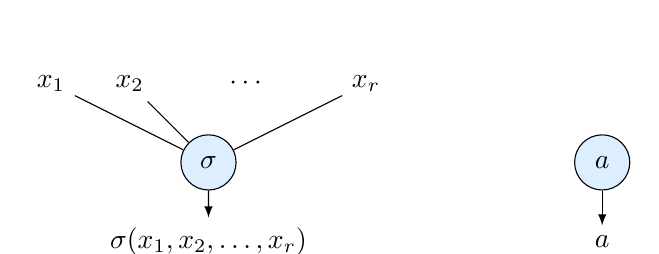
\begin{tikzpicture}
\draw (-2, 2) node(x1) {$x_1$} ;
\draw (-1, 2) node(x2) {$x_2$} ;
\draw (0.5, 2) node(dots) {$\cdots$} ;
\draw (2, 2) node(xr) {$x_r$} ;
  \draw (0, 1) \sdconstructor{sigma}{$\sigma$} ;
    \draw (0, 0) node(result) {$\sigma(x_1,x_2,\dots,x_r)$} ;
\draw[-latex] (x1) -- (sigma) -- (result) ;
\draw (x2) -- (sigma) ;
\draw (xr) -- (sigma) ;
\draw (5,1) \sdconstructor{a}{$a$} ;
  \draw (5,0) node(aresult) {$a$} ;
\draw[-latex] (a) -- (aresult) ;
\end{tikzpicture}
\end{center}

Thus the rules $0 = (~ \mid 0)$ and $s = (n \mid n+1)$ that describe the natural numbers can be expressed as follows:
\begin{center}
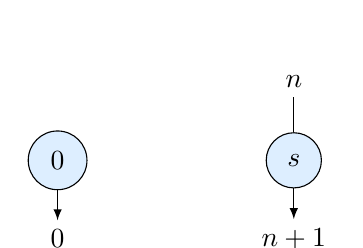
\begin{tikzpicture}
\draw (0,1) \sdconstructor{c0}{$0$} ;
  \draw (0,0) node(n0) {$0$} ;
\draw (3,2) node(varn) {$n$} ;
  \draw (3,1) \sdconstructor{s}{$s$} ;
    \draw (3,0) node(varsn) {$n+1$} ;
\draw[-latex] (c0) -- (n0) ;
\draw[-latex] (varn) -- (s) -- (varsn) ;
\end{tikzpicture}
\end{center}

These diagrams can be pieced together to represent the result of applying a rule to the outputs of other rules. For example:
\begin{center}
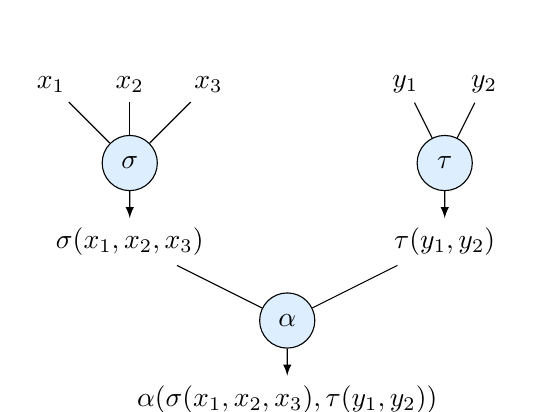
\begin{tikzpicture}
\draw (-3,4) node(a) {$x_1$} ;
\draw (-2,4) node(b) {$x_2$} ;
\draw (-1,4) node(c) {$x_3$} ;
  \draw (-2,3) \sdconstructor{sigma}{$\sigma$} ;
    \draw (-2,2) node(sigmares) {$\sigma(x_1,x_2,x_3)$} ;
\draw (1.5,4) node(x) {$y_1$} ;
\draw (2.5,4) node(y) {$y_2$} ;
  \draw (2,3) \sdconstructor{tau}{$\tau$} ;
    \draw (2,2) node(taures) {$\tau(y_1,y_2)$} ;
      \draw (0,1) \sdconstructor{alpha}{$\alpha$} ;
        \draw (0,0) node(alphares) {$\alpha(\sigma(x_1,x_2,x_3), \tau(y_1,y_2))$} ;
\draw[-latex] (a) -- (sigma) -- (sigmares) ;
\draw (b) -- (sigma) ;
\draw (c) -- (sigma) ;
\draw[-latex] (x) -- (tau) -- (taures) ;
\draw (y) -- (tau) ;
\draw[-latex] (sigmares) -- (alpha) -- (alphares) ;
\draw (taures) -- (alpha) ;
\end{tikzpicture}
\end{center}

This can be useful for seeing how an element of a set is obtained by applying the rules. For example, the following diagram shows how the natural number $3$ is obtained by applying the rules $(~ \mid 0)$ and $(n \mid n+1)$

\begin{center}
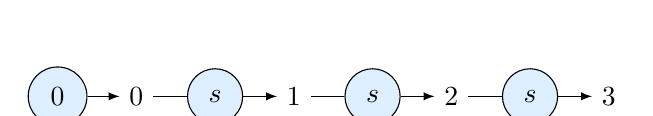
\begin{tikzpicture}
\draw (0,0) \sdconstructor{c0}{$0$} ;
  \draw (1,0) node(n0) {$0$} ;
    \draw (2,0) \sdconstructor{s1}{$s$} ;
      \draw (3,0) node(n1) {$1$} ;
        \draw (4,0) \sdconstructor{s2}{$s$} ;
          \draw (5,0) node(n2) {$2$} ;
            \draw (6,0) \sdconstructor{s3}{$s$} ;
              \draw (7,0) node(n3) {$3$} ;
\draw[-latex] (c0) -- (n0) ;
\draw[-latex] (n0) -- (s1) -- (n1);
\draw[-latex] (n1) -- (s2) -- (n2) ;
\draw[-latex] (n2) -- (s3) -- (n3) ;
\end{tikzpicture}
\end{center}

The following diagram shows how the logical formula $(p \Rightarrow q) \wedge (\neg r)$ is obtained by applying the rules described in \Cref{exRulesForInductiveDefinitionOfPropositionalFormulae}.

\begin{center}
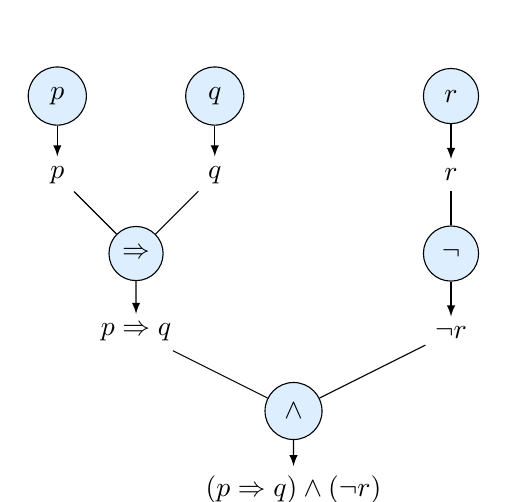
\begin{tikzpicture}
\draw (-3,5) \sdconstructor{cp}{$p$} ;
\draw (-1,5) \sdconstructor{cq}{$q$} ;
\draw (2,5) \sdconstructor{cr}{$r$} ;
\draw (-3,4) node(p) {$p$} ;
\draw (-1,4) node(q) {$q$} ;
  \draw (-2,3) \sdconstructor{implies}{$\Rightarrow$} ;
    \draw (-2,2) node(pimpliesq) {$p \Rightarrow q$} ;
\draw (2,4) node(r) {$r$} ;
  \draw (2,3) \sdconstructor{not}{$\neg$} ;
    \draw (2,2) node(notr) {$\neg r$} ;
      \draw (0,1) \sdconstructor{and}{$\wedge$} ;
        \draw (0,0) node(result) {$(p \Rightarrow q) \wedge (\neg r)$} ;
\draw[-latex] (cp) -- (p) ;
\draw[-latex] (cq) -- (q) ;
\draw[-latex] (cr) -- (r) ;
\draw[-latex] (p) -- (implies) -- (pimpliesq) ;
        \draw (q) -- (implies) ;
\draw[-latex] (r) -- (not) -- (notr) ;
\draw[-latex] (pimpliesq) -- (and) -- (result) ;
        \draw (notr) -- (and) ;
\end{tikzpicture}
\end{center}

\begin{exercise}
Let $\Sigma = \{ a,b,c,d \}$. Draw a diagram to represent how the word $cbadbd \in \Sigma^*$ can be obtained by applying the rules you defined in \Cref{exRulesForInductiveDefinitionOfWords}.
\end{exercise}

We are now ready to define an inductively defined set.

\begin{definition}
\label{defInductivelyDefinedSet}
\index{inductively defined set}
\index{set!inductively defined}
\index{constructor}
An \textbf{inductively defined set} is a set $A$ equipped with a set $R$ of rules and, for each rule $\sigma = (x_1,x_2,\dots,x_r \mid \sigma(x_1,x_2,\dots,x_r)) \in R$, a function $f_{\sigma} : A^r \to A$, such that:
\begin{enumerate}[(a)]
\item For each $a \in A$, there is a unique rule $\sigma \in R$ and unique elements $a_1,a_2,\dots,a_r \in A$ such that $a = f_{\sigma}(a_1,a_2,\dots,a_r)$; and
\item For every set $X$, if $f_{\sigma}(a_1,a_2,\dots,a_r) \in X$ for all $\sigma \in R$ and all $a_1,a_2,\dots,a_r \in A$, then $A \subseteq X$.
\end{enumerate}
Given a rule $\sigma$ of arity $r$, the functions $f_{\sigma} : A^r \to A$ is called the \textbf{constructor} associated with $\sigma$; the natural number $r$ is called the \textbf{arity} of the constructor.
\end{definition}

Note that nullary constructors are the same thing as elements of $A$. Indeed, $A^0 = \{ () \}$, where $()$ is the empty list of elements of $A$, and so specifying a function $f_{\sigma} : A^0 \to A$ is equivalent to specifying an element $f_{\sigma}(\,()\,) \in A$. In this sense, we may regard nullary constructors as \textit{being} the elements of $A$---we call such elements \textit{basic elements}.

\begin{definition}
\label{defBasicElement}
\index{basic element}
\index{element!basic}
A \textbf{basic element} of an inductively defined set $A$ is an element of $A$ that is the value of a nullary constructor $f_{\sigma} : A^0 \to A$. If $\sigma = (~ \mid a)$ is a nullary rule, we will denote this element by $a$---thus we have $a = f_{\sigma}(\,()\,) \in A$ for all nullary rules $\sigma = (~ \mid a)$.
\end{definition}

Considering basic elements separately from constructors of positive arity has its pros and cons, so we will take whichever approach is most convenient for us at any given point in time. Unless otherwise specified, we will not separate nullary constructors from the others.

We have already seen some examples of inductively defined sets---let's prove that they truly \textit{are} inductively defined sets!

\begin{proposition}
\label{propNIsInductivelyDefined}
The set $\mathbb{N}$ of natural numbers is inductively defined by the rules $(~ \mid 0)$ and $(n \mid n+1)$.
\end{proposition}

\begin{cproof}
Since $(~ \mid 0)$ is a nullary rule, it will correspond to a basic element of $\mathbb{N}$---it may be no surprise that we take this element to be the natural number $0$.

The rule $s = (n \mid n+1)$ induces a function $f_s : \mathbb{N} \to \mathbb{N}$; we take this to be the successor function, defined by $f_s(n) = n+1$ for all $n \in \mathbb{N}$.

Now we must verify conditions (a) and (b) of \Cref{defInductivelyDefinedSet}.
\begin{enumerate}[(a)]
\item Let $n \in \mathbb{N}$.
\begin{itemize}
\item If $n = 0$, then since $0$ is a basic element and $0 \ne n+1 = f_s(n)$ for any $n \in \mathbb{N}$, we have that `$0$' is the unique expression of $0$ as a (nullary) constructor applied to (no) elements of $\mathbb{N}$.
\item If $n > 0$, then $n-1 \in \mathbb{N}$ and $n = (n-1)+1 = f_s(n-1)$. Moreover if $m \in \mathbb{N}$ and $n=f_s(m)$, then $n=m+1$, so that $m=n-1$. Moreover $n \ne 0$, meaning that there is a unique rule (namely $s$) and a unique natural number $m$ (namely $m=n-1$) such that $n=f_s(m)$.
\end{itemize}
\item Let $X$ be a set, and assume that $0 \in X$ and $f_s(n) \in X$ for all $n \in \mathbb{N}$. Then condition (iii) of \Cref{defNotionOfNaturalNumbers} ensures that $\mathbb{N} \subseteq X$.
\end{enumerate}

Thus $\mathbb{N}$ is inductively defined by $(~ \mid 0)$ and $(n \mid n+1)$, as required.
\end{cproof}

\begin{example}
\label{exInductivelyDefinedSetOfPropositionalFormulae}
Let $P$ be a set of propositional variables. In order to exhibit $L(P)$ as an inductively defined set, we should be slightly more precise about the role of \textit{brackets} in propositional formulae than we have been so far.

For example, if we take the rules discussed in \Cref{exPropositionalFormulaeAsInductivelyDefinedSetPreliminary} literally, then $p \wedge q \vee r$ would be a valid logical formula. This is problematic for two reasons: first, does it mean $(p \wedge q) \vee r$, or $p \wedge (q \vee r)$? These are not logically equivalent, so the distinction matters. Second, this causes the `uniqueness' part of \Cref{defInductivelyDefinedSet} to fail, since $p \wedge q \vee r = f_{\wedge}(p,f_{\vee}(q,r)) = f_{\vee}(f_{\wedge}(p,q),r)$.

To remedy this, we will require parentheses to be added whenever we introduce a logical operator. Thus the rules defining a logical formula are:
\[ \underbrace{({-} \mid p)}_{\text{one for each } p \in P} \quad (\varphi,\psi \mid (\varphi \wedge \psi)\,) \quad (\varphi,\psi \mid (\varphi \vee \psi)\,) \quad (\varphi,\psi \mid (\varphi \Rightarrow \psi)\,) \quad (\varphi \mid (\neg \varphi)\,) \]

Thus $p \wedge q \vee r$ is not a valid element of $L(P)$, but $((p \wedge q) \vee r)$ and $(p \wedge (q \vee r))$ are.
\end{example}

\begin{exercise}
Let $\Sigma$ be an alphabet. Prove that $\Sigma^*$ is inductively defined by the rules $(~ \mid \varepsilon)$ and $\sigma_a = (w \mid wa)$ for $a \in \Sigma$.
\end{exercise}

\begin{exercise}
Prove that $\mathbb{N}$ is generated by the rules $(~ \mid 0)$, $(~ \mid 1)$ and $(~ \mid n+2)$.
\end{exercise}

\subsection*{Defining new inductively defined sets}

Now that we have seen what it means for a set to \textit{be} inductively defined, it would be useful to be able to \textit{make definitions} of inductively defined sets. Based on what we have seen so far, in order to define an inductively defined set, all we should need to do is specify a set of rules that tell us how to generate its elements.

We now prove that it really is that simple!

\begin{definition}
\label{defSetGeneratedByRules}
Let $R$ be a set of rules. The set \textbf{generated by} $R$ is defined by $A = \bigcup_{n \in \mathbb{N}} A_n$, where the sets $A_n$ for $n \in \mathbb{N}$ are defined recursively by:
\[ A_0 = \left\{ a \middlemid (~\mid a) \in R \right\} \]
and
\[ A_{n+1} = \left\{ \sigma(a_1,a_2,\dots,a_r) \middlemid a_1,a_2,\dots,a_r \in A_n, ~ (x_1,x_2,\dots,x_r \mid \sigma(x_1,x_2,\dots,x_r) \in R \right\} \]
That is, $A_0$ is the set of symbols to the right of the bar `$\mid$' in the nullary rules in $R$, and $A_{n+1}$ is the set of all expressions obtained by substituting the elements of $A_n$ symbol-by-symbol for the variables in the expressions to the right of the bar the other rules.
\end{definition}

\begin{example}
Let $N$ be the set generated by the rules $(~ \mid z)$ and $(n \mid s(n))$. Then
\begin{itemize}
\item $N_0 = \{ z \}$, since $(~ \mid z)$ is the only nullary rule.
\item $N_1$ is the result of applying the rules to the elements of $N_0$, of which there is only one, namely $z$. Applying the rule $(~\mid z)$ (to no elements, since it is nullary) gives $z$; applying the rule $(n \mid s(n))$ to $z$ gives $s(z)$. So $N_1 = \{ z, s(z) \}$.
\item Continuing, we get $N_2 = \{ z, s(z), s(s(z)) \}$, and so on.
\end{itemize}
We thus have
\[ N ~=~ \bigcup_{n \in \mathbb{N}} N_n ~=~ \{ z, s(z), s(s(z)), s(s(s(z))), \dots \} \]
This looks an awful lot like the set of all natural numbers; and indeed it is, provided we interpret $z=0$ and $s(n)=n+1$ (like we did in \Cref{secPeanosAxioms}).
\end{example}

\begin{example}
\label{exParenthesisations}
Let $A$ be the set generated by the rules $(~ \mid \star)$ and $(x,y \mid [x,y])$. Then
\begin{itemize}
\item $A_0 = \{ \star \}$;
\item $A_1 = \{ \star,~ [\star, \star] \}$;
\item $A_2 = \{ \star,~ [\star, \star],~ [\star, [\star,\star]],~ [[\star, \star], \star],~ [[\star,\star],[\star,\star]] \}$;
\item \dots{} and so on.
\end{itemize}
Thus for each $n \in \mathbb{N}$, the set $A_n$ consists of all parenthesised lists of `$\star$'s, where the list has length between $1$ and $2^n$ (inclusive). This can be proved by induction on $n$.

Hence $A = \bigcup_{n \in \mathbb{N}} A_n$ is the set of all (finite) such lists.
\end{example}

\begin{exercise}
Let $R$ be a set of rules for an inductive definition and let $A$ be the set generated by $R$. Prove that if $R$ has no nullary rules, then $A$ is empty.
\end{exercise}

\begin{exercise}
Let $R$ be a set of rules for an inductive definition, and let $A$ be the set generated by $R$. Prove that if $R$ is countable, then $A$ is countable.
\end{exercise}

\begin{exercise}
\label{exSetGeneratedByRulesIsInductivelyDefined}
Let $R$ be a set of rules. Prove that the set $A$ generated by $R$ is inductively defined; for each rule $\sigma = (x_1,x_2,\dots,x_r \mid \sigma(x_1,x_2,\dots,x_r))$, the constructor $f_{\sigma} : A^r \to A$ is defined by
\[ f_{\sigma}(a_1,a_2,\dots,a_r) ~=~ \sigma(a_1,a_2,\dots,a_r) \]
where $\sigma(a_1,a_1,\dots,a_r)$ denotes the result of substituting $a_i$ for the variable $x_i$ for each $i \in [r]$.
\end{exercise}

\subsection*{Structural recursion}

The recursion theorem for the natural numbers (\Cref{thmRecursion}) says that we can define a function $h : \mathbb{N} \to X$ by specifying the value of $h(0)$, and for each $n \in \mathbb{N}$, specifying the value of $h(n+1)$ in terms of the value of $h(n)$. This makes intuitive sense: since every natural number is obtained from $0$ by adding one some finite number of times, if we know the value of $h(0)$, and we know how the value of $h$ changes when we add one to its argument, then we should know the value of $h(n)$ for all natural numbers $n$.

It turns out that there is nothing special about $\mathbb{N}$ here: exactly the same argument demonstrates that for \textit{any} inductively defined set $A$, if we know what a function $h : A \to X$ does to its basic elements, and we know how its values change when we apply a constructor to its arguments, then we should know the value of $h(a)$ for all $a \in A$.

The proof of the structural recursion theorem is one of the times where treating basic elements ($\equiv$ nullary constructors) separately from constructors of positive arity makes the proof more difficult; so we will phrase it entirely in terms of constructors.

\begin{theorem}[Structural recursion theorem]
\label{thmStructuralRecursion}
Let $A$ be an inductively defined set, let $X$ be a set, and for each rule $\sigma$, let $h_{\sigma} : A^r \to X$ be a function, where $r = \mathrm{ar}(\sigma)$. Then there is a unique function $h : A \to X$ such that
\[ h(f_{\sigma}(a_1,a_2,\dots,a_r)) ~=~ h_{\sigma}(a_1,a_2,\dots,a_r) \]
for all rules $\sigma$ and all $a_1,a_2,\dots,a_r \in A$.
\end{theorem}

\begin{cproof}
Given $a \in A$, we know by \Cref{defInductivelyDefinedSet}(a) that there is a unique rule $\sigma$ and unique $a_1,a_2,\dots,a_r \in A$ such that $a = f_{\sigma}(a_1,a_2,\dots,a_r)$. Thus the specification
\[ h(a) ~=~ h_{\sigma}(a_1,a_2,\dots,a_r) \]
uniquely determines a function $h : A \to X$, satisfying the required condition.
\end{cproof}

\begin{strategy}[Defining functions by structural recursion]
\label{strStructuralRecursion}
Let $A$ be an inductively defined set and let $X$ be a set. In order to specify a function $h : A \to X$, it suffices to define $h(a)$ for all basic elements $a \in A$, and to define $h(f_{\sigma}(a_1,a_2,\dots,a_r))$ in terms of the values of $h(a_i)$ for each $i \in [r]$.
\end{strategy}

\begin{example}
Let $L(P)$ be the inductively defined set of propositional formulae over a set $P$ of propositional variables. Define $h : L(P) \to \mathbb{N}$ recursively as follows:
\begin{enumerate}[(i)]
\item Let $h(p) = 0$ for all $p \in P$;
\item For all $\varphi, \psi \in L(P)$, let $h(\varphi \wedge \psi) = h(\varphi) + h(\psi) + 1$;
\item For all $\varphi, \psi \in L(P)$, let $h(\varphi \vee \psi) = h(\varphi) + h(\psi) + 1$;
\item For all $\varphi, \psi \in L(P)$, let $h(\varphi \Rightarrow \psi) = h(\varphi) + h(\psi) + 1$;
\item For all $\varphi \in L(P)$, let $h(\neg \varphi) = h(\varphi) + 1$.
\end{enumerate}
By the structural recursion theorem, this completely determines the function $h$.

For example
\begin{align*}
& h((p \Rightarrow q) \wedge (\neg r)) && \\
&= h(p \Rightarrow q) + h(\neg r) + 1 && \text{by (ii)} \\
&= [h(p) + h(q) + 1] + [h(r) + 1] + 1 && \text{by (iv) and (v)} \\
&= [0+0+1] + [0+1] + 1 && \text{by (i)} \\
&= 3
\end{align*}

More generally, for each $\varphi \in L(P)$, the value $h(\varphi)$ is the number of logical operators that appear in $\varphi$. We can prove this by \textit{structural induction}---more on this soon.
\end{example}

\begin{definition}
\label{defRank}
\index{rank}
\nindex{rk}{$\mathrm{rk}(a)$}{rank}
Let $A$ be an inductively defined set. The \textbf{rank} $\mathrm{rk}(a)$ \inlatex{mathrm\{rk\}}\lindexmmc{mathrm}{$\mathrm{Aa, Bb, Cc, \dots}$} of an element $a \in A$ is defined by recursively by letting $\mathrm{rk}(a) = 0$ for all basic elements $a$, and
\[ \mathrm{rk}(f_{\sigma}(a_1,a_2,\dots,a_r)) = \mathrm{max} \{ \mathrm{rk}(a_1), \mathrm{rk}(a_2),\dots, \mathrm{rk}(a_r) \} + 1 \]
for all rules $\sigma$ of arity $r>0$ and all elements $a_1,a_2,\dots,a_r \in A$.
\end{definition}

\begin{example}
The rank of a natural number $n$ is $n$. Indeed we have $\mathrm{rk}(0) = 0$ since $0$ is a basic element, and for all $n \in \mathbb{N}$ we have $\mathrm{rk}(n+1) = \mathrm{max} \{ \mathrm{rk}(n) \} + 1 = \mathrm{rk}(n) + 1$. By the recursion theorem (take your pick from \Cref{thmRecursion} or \Cref{thmStructuralRecursion}), we have $\mathrm{rk}(n) = n$ for all $n \in \mathbb{N}$.
\end{example}

\begin{exercise}
Let $\Sigma$ be an alphabet and let $\Sigma^*$ be the inductively defined set of words over $\Sigma$. Prove that for all $w \in \Sigma$, the rank $\mathrm{rk}(w)$ is equal to the length of $W$. [We regard the empty string $\varepsilon$ to have length $0$, despite the fact that the placeholder character $\varepsilon$ is used to denote it.]
\end{exercise}

\subsection*{Structural induction}

We now derive the structural induction principle, which is used for proving that a property $p(x)$ is true for all elements $x$ of an inductively defined set $A$.

The idea behind structural induction is the same as the idea behind weak induction: since every element $a \in A$ is of the form $f_{\sigma}(a_1,a_2,\dots,a_r)$ for some (possibly nullary) rule $\sigma$, if we can prove that the truth of $p$ is preserved by applying each constructor $f_{\sigma}$, then $p(x)$ must be true for all $x \in A$. [In the nullary case, this amounts to checking that $p(a)$ is true for each basic element $a \in A$.]

Thus in order to prove $\forall x \in A,~ p(x)$, we need to prove that for every rule $\sigma$\dots{}

\begin{center}
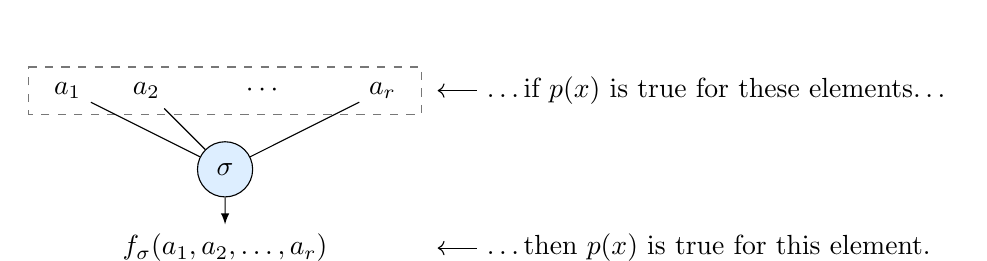
\begin{tikzpicture}
\draw (-2, 2) node(x1) {$a_1$} ;
\draw (-1, 2) node(x2) {$a_2$} ;
\draw (0.5, 2) node(dots) {$\cdots$} ;
\draw (2, 2) node(xr) {$a_r$} ;
  \draw (0, 1) \sdconstructor{sigma}{$\sigma$} ;
    \draw (0, 0) node(result) {$f_{\sigma}(a_1,a_2,\dots,a_r)$} ;
\draw[<-] (2.7, 2) -- (3.2,2) node[right] {\dots{}if $p(x)$ is true for these elements\dots{}} ;
\draw[<-] (2.7, 0) -- (3.2,0) node[right] {\dots{}then $p(x)$ is true for this element.} ;
\draw[midgray, dashed] (-2.5,2.3) -- (2.5,2.3) -- (2.5,1.7) -- (-2.5,1.7) -- cycle ;
\draw[-latex] (x1) -- (sigma) -- (result) ;
\draw (x2) -- (sigma) ;
\draw (xr) -- (sigma) ;
\end{tikzpicture}
\end{center}

Let's prove that this intuition is valid.

\begin{theorem}[Structural induction principle]
\label{thmStructuralInduction}
\index{induction!structural}
Let $A$ be an inductively defined set and let $p(x)$ be a logical formula with free variable $x \in A$. If for all rules $\sigma$ and all $a_1,\dots,a_r \in A$ we have
\[ [\forall i \in [r],~ p(a_i)] \Rightarrow f_{\sigma}(a_1,a_2,\dots,a_r) \]
then $p(x)$ is true for all $x \in A$.
\end{theorem}

\begin{cproof}
Assume that for all rules $\sigma$ and all $a_1,\dots,a_r \in A$ we have
\[ [p(a_1) \wedge p(a_2) \wedge \cdots \wedge p(a_r)] \Rightarrow p(f_{\sigma}(a_1,a_2,\dots,a_r)) \]

Let $X = \{ a \in A \mid p(a) \} \subseteq A$. Then for all $a \in A$ we have $a \in X$ if and only if $p(a)$ is true. Thus we have
\[ [\forall i \in [r],~ p(i)] \Rightarrow f_{\sigma}(a_1,a_2,\dots,a_r) \in X \]
But this is exactly the hypothesis of condition (b) of \Cref{defInductivelyDefinedSet}, and so $A \subseteq X$.

Hence $A = X$, so that $p(a)$ is true for all $a \in A$, as required.
\end{cproof}

Let's digest the statement of \Cref{thmStructuralInduction}.

For a nullary rule $\sigma = (~ \mid a)$, the arity $r$ is $0$, so $\forall i \in [r],~p(a_i)$ is vacuously true (see \Cref{exEverythingIsTrueOfElementsOfEmptySet}), so that
\[ [\forall i \in [r],~ p(a_i)] \Rightarrow p(f_{\sigma}(a_1,a_2,\dots,a_r)) \quad \equiv \quad p(a) \]

Therefore, saying that $[\forall i \in [r],~ p(a_i)] \Rightarrow f_{\sigma}(a_1,a_2,\dots,a_r)$ is true for all rules $\sigma$ and all elements $a_1,a_2,\dots,a_r \in A$ is equivalent to saying:
\begin{itemize}
\item $p(a)$ is true for all basic elements $a$; and
\item $[\forall i \in [r],~ p(a_i)] \Rightarrow f_{\sigma}(\sigma(a_1,a_2,\dots,a_r))$ is true for all rules $\sigma$ of \textit{positive} arity $r$, and all elements $a_1,a_2,\dots,a_r$.
\end{itemize}

This suggests the following proof strategy.

\begin{strategy}[Proof by structural induction]
\index{proof!by structural induction}
\index{induction!on an inductively defined set}
In order to prove a proposition of the form $\forall a \in A,~ p(a)$, where $A$ is an inductively defined set, it suffices to prove for all rules $\sigma$ that
\[ [p(a_1) \wedge p(a_2) \wedge \cdots \wedge p(a_r)] \Rightarrow p(f_{\sigma}(a_1,a_2,\dots,a_r)) \]
Equivalently, it suffices to:
\begin{itemize}
\item For each basic element $a \in A$, prove $p(a)$---this is the \textbf{base case} for $a$;
\item For each constructor $\sigma$ of arity $r>0$, let $a_1,a_2,\dots,a_r \in A$ and assume that $p(a_i)$ is true for all $i \in [r]$, and prove that $p(f_{\sigma}(a_1,a_2,\dots,a_r))$ is true---this is the \textbf{induction step} for $\sigma$.
\end{itemize}
The assumption $p(a_1,a_2,\dots,a_r)$ in the induction step for $\sigma$ is called the \textbf{induction hypothesis} for $\sigma$.
\end{strategy}

\begin{example}
The structural induction principle for the inductively defined set $\mathbb{N}$ is exactly the same as the weak induction principle (\Cref{thmWeakInduction}). It says that to prove $\forall n \in \mathbb{N},~ p(n)$ is true, it suffices to:
\begin{itemize}
\item Prove $p(0)$ is true (since $0$ is the only basic element); and
\item Let $n \in \mathbb{N}$, assume that $p(n)$ is true, and prove that $p(n+1)$ is true (since the successor operation is the only constructor of positive arity).
\end{itemize}
Thus we recover weak induction as a special case of structural induction.
\end{example}

\begin{example}
Fix a set $P$ of propositional variables and let $L(P)$ be the inductively defined set of (properly parenthesised) propositional formulae over $P$, as in \Cref{exInductivelyDefinedSetOfPropositionalFormulae}.

We prove that every propositional formula $\varphi \in L(P)$ has the same number of open brackets `$($' as closed brackets `$)$'.

\begin{itemize}
\item (\textbf{Base cases}) The basic elements of $L(P)$ are the propositional variables $p \in P$. So let $p \in P$; this is a logical formula with no open brackets and no closed brackets, so the number of open brackets is equal to the number of closed brackets.

\item (\textbf{Induction step} for $\wedge$) Let $\varphi, \psi \in L(P)$ and assume that $\varphi$ and $\psi$ each have the same number of open brackets as closed brackets. Say $\varphi$ has $a$ open brackets and $a$ closed brackets, and $\psi$ has $b$ open brackets and $b$ closed brackets, where $a,b \in \mathbb{N}$. Now
\[ f_{\wedge}(\varphi, \psi) ~=~ (\varphi \wedge \psi) \]
Since $\varphi$ contributes $a$ open brackets and $\psi$ contributes $b$ open brackets, this has $a+b+1$ open brackets; likewise it has $a+b+1$ closed brackets.

This completes the induction step for $\wedge$.

\item (\textbf{Induction steps} for $\vee$ and $\Rightarrow$) These are identical to the induction step for $\wedge$---just replace $\wedge$ by the necessary logical operator throughout.

\item (\textbf{Induction step} for $\neg$) Let $\varphi \in L(P)$ and assume that $\varphi$ has the same number of open brackets as closed brackets---say it has $a$ of each, where $a \in \mathbb{N}$. Then
\[ f_{\neg}(\varphi) ~=~ (\neg \varphi) \]
Since $\varphi$ contributes $a$ open brackets, this has $a+1$ open brackets; likewise it has $a+1$ closed brackets.

This completes the induction step for $\neg$.
\end{itemize}

So by structural induction, it follows that every propositional formula $\varphi \in L(P)$ has the same number of open brackets as closed brackets.
\end{example}

\begin{exercise}
Let $P$ be a set of propositional variables. Prove by structural induction that the rank of a propositional formula $\varphi \in L(P)$ is equal to the number of logical operators in $\varphi$.
\end{exercise}

A nice application of structural induction is to provide a formula for the \textit{totient} of an integer $n$ (\Cref{defTotient}). We proved such a formula in \Cref{secModularArithmetic}, but that proof relied on the heavy machinery of the Chinese remainder theorem (\Cref{thmChineseRemainder})---here we give a proof without it.

\rthmTotientFormula*

\begin{cproof}
%% BEGIN EXTRACT (xtrWlogExample) %%
Recall that $\varphi(-n) = \varphi(n)$ for all $n \in \mathbb{Z}$, so we may assume without loss of generality that $n \ge 0$---otherwise just replace $n$ by $-n$ throughout.
%% END EXTRACT %%
Moreover
\[ \varphi(0) ~=~ 0 ~=~ 0 \cdot \prod_{p \mid n} \left( 1- \frac{1}{p} \right) \]
so for the rest of the proof, assume that $n>0$.

Let $P$ be the set of all positive prime numbers, and let
\[ A ~=~ \bigcup_{n \in \mathbb{N}} P^n ~=~ \{ (p_1,p_2,\dots,p_k) \mid k \in \mathbb{N},~ p_1,p_2,\dots,p_k \in P \} \]
The elements of $A$ are precisely lists of positive primes of finite length. Note that $A$ is inductively defined by the rules
\[ (~ \mid ()\,) \quad \text{and} \quad \sigma_q = (x \mid (x,q)) \text{ for each } q \in P \]
That is, the empty list $()$ is an element of $A$, and for each $(p_1,p_2,\dots,p_k) \in A$ and $q \in P$, we have $(p_1,p_2,\dots,p_k,q) \in A$.

By the fundamental theorem of arithmetic (\Cref{thmFTA}) there is a surjection $\Pi : A \to \{ n \in \mathbb{Z} \mid n > 0 \}$ defined by
\[ \Pi(p_1,p_2,\dots,p_k) ~=~ \prod_{i=1}^k p_i ~=~ p_1 \times p_2 \times \cdots \times p_k \]
for all $k \in \mathbb{N}$ and $p_1,p_2,\dots,p_k \in P$. Note in particular that $\Pi(\,()\,) = 1$, where $()$ is the empty list.

We prove by structural induction on $(p_1,p_2,\dots,p_k) \in A$ that the integer $n = \Pi(p_1,p_2,\dots,p_k) > 0$ satisfies the formula in the statement of the theorem. 

\begin{itemize}
\item (\textbf{Base case}) The unique basic element of $A$ is the empty list $()$. Since $\Pi(\,()\,) = 1$, we must prove that the equation in the statement of the theorem is satisfied when $n=1$. Well there are no primes $p$ such that $p \mid 1$, and so the product $\prod_{p \mid 1} \left( 1 - \frac{1}{p} \right)$ is the empty product, which is equal to $1$. Thus
\[ \varphi(1) ~=~ 1 ~=~ 1 \cdot 1 ~=~ 1 \cdot \prod_{p \mid 1} \left( 1- \frac{1}{p} \right) \]
as required.

\item (\textbf{Induction step} for $q \in P$) Fix $(p_1,p_2,\dots,p_k) \in A$, let $n = \Pi(p_1,p_2,\dots,p_k)$ and assume that
\[ \varphi(n) ~=~ n \cdot \prod_{p \mid n} \left( 1 - \frac{1}{p} \right) \]
Note that $\Pi(p_1,p_2,\dots,p_k,q) = qn$, and so we need to prove that
\[ \varphi(qn) ~=~ qn \cdot \prod_{p \mid qn} \left( 1 - \frac{1}{p} \right) \]
Now either $q \mid n$ or $q \nmid n$.
\begin{itemize}
\item Assume $q \mid n$. Then $n$ and $qn$ have the same prime divisors, and so for all $p \in P$ we have $p \mid n$ if and only if $p \mid qn$. Therefore:
\begin{align*}
\varphi(qn) &= q\varphi(n) && \text{by \Cref{exTotientMultiplyByPrime}} \\
&= qn \cdot \prod_{p \mid n} \left( 1-\frac{1}{p} \right) && \text{by induction hypothesis} \\
&= qn \cdot \prod_{p \mid qn} \left( 1-\frac{1}{p} \right) && \text{as observed above}
\end{align*}
as required.

\item Assume $q \nmid n$. Then for all $p \in P$ we have $p \mid qn$ if and only if $p \mid n$ or $p=q$. Therefore:
\begin{align*}
\varphi(qn) &= (q-1)\varphi(n) && \text{by \Cref{exTotientMultiplyByPrimeTwo}} \\
&= (q-1) n \cdot \prod_{p \mid n} \left( 1 - \frac{1}{p} \right) && \text{by induction hypothesis} \\
&= qn \left( 1 - \frac{1}{q} \right) \cdot \prod_{p \mid n} \left( 1 - \frac{1}{p} \right) && \text{rearranging} \\
&= qn \cdot \prod_{p \mid qn} \left( 1 - \frac{1}{p} \right) && \text{absorbing $1-\frac{1}{q}$ into the product}
\end{align*}

as required.
\end{itemize}

In both cases, the formula in the statement of the theorem is satisfied by the integer $qn$.
\end{itemize}

By structural induction, the result follows.
\end{cproof}

\subsection*{Uniqueness of inductive definitions}

It would be nice if an inductive definition completely characterises the set that it defines. But this is slightly too much to ask; for example, the sets
\[ \{ 0, 1, 2, 3, \dots \} \quad \text{and} \quad \{ \varepsilon, {\bullet}, {\bullet} {\bullet}, {\bullet} {\bullet} {\bullet}, \dots \} \]
are both inductively defined by the rules $(~ \mid z)$ and $(n \mid s(n))$. In the first we take the basic element $z$ to be the natural number $0$, and for each natural number $n$ we take $s(n)$ to be the natural number $n+1$; in the second, we take the basic element $z$ to be the empty word $\varepsilon$, and for each string $n$ we take $s(n)$ to be the string `$n {\bullet}$' (so for example $s({\bullet} {\bullet}) = {\bullet} {\bullet} {\bullet}$).

But there is evidently a way of translating between these sets: we can define a function from the first to the second by sending each natural number $n$ to the string ${\bullet} {\bullet} \cdots {\bullet}$, where there are $n$ `${\bullet}$'s in the string.

Thus the sets $\{ 0, 1, 2, 3, \dots \}$ and $\{ \varepsilon, {\bullet}, {\bullet}{\bullet}, {\bullet}{\bullet}{\bullet}, \dots \}$ are `essentially the same'---they are inductively defined by the same rules, and so the only real difference is how we \textit{label} their elements.

The next theorem demonstrates that the same is true of inductively defined sets in general. That is, if two sets $A$ and $B$ are inductively defined by the same rules, then the only way that they can differ is in the labels we use to denote their elements. Formally, this `relabelling' establishes a bijection $h : A \to B$ between the two sets.

In fact, we prove something stronger: not only is there a bijection between the two sets, but the bijection respects the constructors---that is, if we apply a constructor in $A$ to some elements and relabel the result, that is equivalent to relabelling the elements first and then applying the corresponding constructor in $B$. Even better, this bijection is the unique bijection that does so.

Thus to sum up what the following theorem tells us: inductively defined sets are \textit{uniquely} determined by their defining rules, up to a \textit{unique} bijection that is compatible with the constructors---this is as close to absolute uniqueness as we could possibly hope to get!

\begin{theorem}[Uniqueness of inductively defined sets]
\label{thmUniquenessOfInductivelyDefinedSets}
Let $A$ and $B$ be two sets that are inductively defined by the same set of rules. There is a unique bijection $h : A \to B$ such that
\[ h(f_{\sigma}(a_1,a_2,\dots,a_r)) ~=~ g_{\sigma}(h(a_1),h(a_2),\dots,h(a_r)) \]
for all rules $\sigma$, where $f_{\sigma} : A^r \to A$ and $g_{\sigma} : B^r \to B$ are the corresponding constructors.
\end{theorem}

\begin{cproof}
Define $h : A \to B$ by structural recursion as follows: given a rule $\sigma$ with arity $r \in \mathbb{N}$ and given $a_1,a_2,\dots,a_r$ such that $h(a_i)$ has been defined for all $i \in [r]$, define
\[ h(f_{\sigma}(a_1,a_2,\dots,a_r)) ~=~ g_{\sigma}(h(a_1),h(a_2),\dots,h(a_r)) \]
We just need to prove that $h$ is a bijection, since evidently the other condition on $h$ is satisfied by construction.

So define $k : B \to A$ by structural recursion on the same way; note that now we have
\[ k(g_{\sigma}(b_1,b_2,\dots,b_r)) ~=~ f_{\sigma}(k(b_1),k(b_2),\dots,k(b_r)) \]

We prove that $k(h(a)) = a$ for all $a \in A$ by structural induction. To this end, let $\sigma$ be a rule of arity $r \in \mathbb{N}$, let $a_1,a_2,\dots,a_r \in A$ and suppose that $k(h(a_i)) = a_i$ for all $i \in [r]$. Let $a = f_{\sigma}(a_1,a_2,\dots,a_r)$. Then
\begin{align*}
k(h(a))
&= k(h(f_{\sigma}(a_1,a_2,\dots,a_r))) && \text{by definition of $a$} \\
&= k(g_{\sigma}(h(a_1),h(a_2),\dots,h(a_r))) && \text{by construction} \\
&= f_{\sigma}(k(h(a_1)),k(h(a_2)),\dots,k(h(a_r)) && \text{by construction} \\
&= f_{\sigma}(a_1,a_2,\dots,a_r) && \text{by induction hypothesis} \\
&= a && \text{by definition of $a$}
\end{align*}
This completes the induction step. So we have $k(h(a)) = a$ for all $a \in A$.

A similar proof by structural induction reveals that $h(k(b)) = b$ for all $b \in B$.

Thus $k$ is an inverse for $h$, so that $h$ is a bijection.

The fact that $h$ is the \textit{unique} such bijection is immediate from the fact that it is defined by structural recursion.
\end{cproof}

\begin{example}
Let $\Sigma$ be an alphabet. Then leaf-labelled rooted planar binary trees over $\Sigma$ are essentially the same as parenthesisations of lists of elements of $\Sigma$ of positive length.

Indeed, let $R$ be the set of rules defined by
\[ R = \{ (~ \mid a) \mid a \in \Sigma \} \cup \{ (t_1,t_2 \mid [t_1,t_2]) \} \]

Like in \Cref{exParenthesisations}, the inductively defined set $A$ generated by $R$ is given by the set of all parenthesisations of lists of elements of $\Sigma$. For example
\[ [[[a_1,a_2],a_3],[a_4,a_5]] \in A \]
where $a_1,a_2,a_3,a_4,a_5 \in \Sigma$.

But the set $T$ of all leaf-labelled rooted planar binary trees over $\Sigma$ is also inductively defined by the rules in $R$. The basic element $a$ corresponding to the rule $(~ \mid a)$ is precisely the tree consisting of just its root, which is labelled by the element $a \in \Sigma$:
\begin{center}
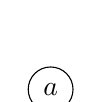
\begin{tikzpicture}
\draw (0,0) node[circle, draw] {$a$} ;
\end{tikzpicture}
\end{center}
and given trees $t_1,t_2$, the tree corresponding to $[t_1,t_2]$ is given by forming a tree with a root and two branches, pasting $t_1$ onto the left branch, and pasting $t_2$ onto the right branch:
\begin{center}
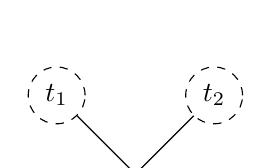
\begin{tikzpicture}
\draw (-1,1) node[circle, dashed, draw](t1) {$t_1$} ;
\draw (1,1) node[circle, dashed, draw](t2) {$t_2$} ;
  \draw[fill=black] (0,0) circle[radius=1.5pt] coordinate(root) ;
\draw (t1) -- (root) -- (t2) ;
\end{tikzpicture}
\end{center}

By \Cref{thmUniquenessOfInductivelyDefinedSets}, there is a unique bijection $A \to T$ that is compatible with the constructors in each set. For example, the element $[[[a_1,a_2],a_3],[a_4,a_5]] \in A$ corresponds with the following tree:
\begin{center}
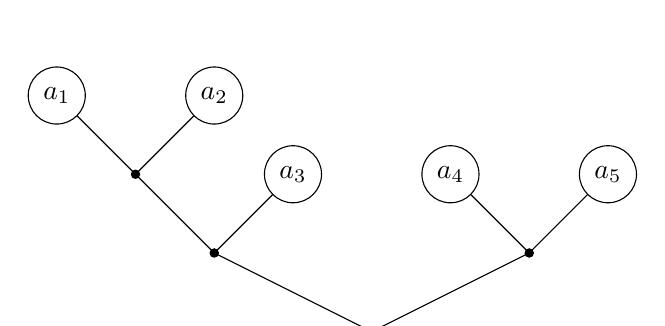
\begin{tikzpicture}
\draw[fill=black] (0,0) circle[radius=1.5pt] coordinate(root) ;
  \draw[fill=black] (-2,1) circle[radius=1.5pt] coordinate(rabc) ;
    \draw[fill=black] (-3,2) circle[radius=1.5pt] coordinate(rab) ;
      \draw (-4,3) node[circle, draw](a) {$a_1$} ;
      \draw (-2,3) node[circle, draw](b) {$a_2$} ;
    \draw (-1,2) node[circle, draw](c) {$a_3$} ;
  \draw[fill=black] (2,1) circle[radius=1.5pt] coordinate(rde) ;
    \draw (1,2) node[circle, draw](d) {$a_4$} ;
    \draw (3,2) node[circle, draw](e) {$a_5$} ;
\draw (root) -- (rabc) -- (rab) -- (a) ;
                    \draw (rab) -- (b) ;
          \draw (rabc) -- (c) ;
\draw (root) -- (rde) -- (d) ;
          \draw (rde) -- (e) ;
\end{tikzpicture}
\end{center}
\end{example}

% \subsection*{Quotient-inductive sets}

% Some sets appear to be inductively defined, except there may be more than one way of expressing each of its elements as a constructor applied to some elements of the set.

% For example, consider the set $\mathbb{Z}$ of integers. Every integer $n$ can be obtained from $0$ by either adding $1$ or subtracting $1$ some number of times. Thus we'd like to say that $\mathbb{Z}$ is generated by the rules
% \[ (~ \mid 0) \quad s = (x \mid x+1) \quad p = (x \mid x-1) \]
% Here $s$ stands for `successor' and $p$ stands for `predecessor'. However, strictly speaking, $\mathbb{Z}$ is not inductively defined by these rules; for example
% \[ 2 = 1 + 1 = f_s(1) \quad \text{and} \quad 2 = 3 - 1 = f_p(3) \]
% and so $2$ does not have a \textit{unique} expression as a constructor applied to an integer.

% In fact, the inductively defined set $A$ generated by the three rules above consists of all strings of the form
% \[ 0 \pm 1 \pm 1 \pm \cdots \pm 1 \]
% with each $\pm$ sign being either $+$ or $-$. We recover the corresponding integer by evaluating the string; this evaluation function defines a \textit{surjection} $q : A \to \mathbb{Z}$; for example
% \[ q(0+1+1) = 2 \quad \text{and} \quad q(0+1+1+1-1+1-1-1+1) = 2 \]
% As made precise in \Cref{thmEquivalenceRelationsSurjections}, the fact that there is a surjection $A \to \mathbb{Z}$ means that we can think of $\mathbb{Z}$ as being a quotient of $A$ by a suitable equivalence relation.

% To see what this equivalence relation is, note that $(n+1)-1 = n$ and $(n-1)+1=n$ for all $n \in \mathbb{Z}$. Thus in a string $0 \pm 1 \pm \cdots \pm 1$, we can add or remove instances of `$+1-1$' or `$-1+1$' in the string as we please, and we will obtain the same integer. So define an equivalence relation $\sim$ on $A$ by letting $a \sim b$ if and only if the string $b$ can be obtained from $a$ by adding or removing `$+1-1$' or `$-1+1$' some number of times; for example
% \[ 0+1+1 \quad \sim \quad 0+1-1+1+1 \quad \sim \quad 0+1+1+1-1+1-1-1+1 \]
% Then $\sim$ is an equivalence relation on $A$, and the evaluation function $q : A \to \mathbb{Z}$ descends to a bijection $\bar q : A/{\sim} \to \mathbb{Z}$.

% We will call sets obtained in this way \textit{quotient-inductive sets}.

\index{induction!structural|)}

% Chapter exercises
\chexbegin{chAdditionalTopics}
\begin{chapex}
For each of the following binary operations on $\mathbb{Z}$, determine whether it is: (i) associative, (ii) unital, (iii) commutative.
\begin{multicols}{2}
\begin{enumerate}[(a)]
\item $a \star b = ab$
\item $a \star b = ab + a + b$
\item $a \star b = a^b$
\item $a \star b = |b - a|$
\item $a \star b = a$
\item $a \star b = a + b + 1$
\end{enumerate}
\end{multicols}
\end{chapex}
\chexend

% Source: LaTeX Stack Exchange
% https://tex.stackexchange.com/q/6489 (Malabarba)
% https://tex.stackexchange.com/a/6494 (Stefan Kottwitz)
% https://tex.stackexchange.com/a/6494#comment971771_6494 (egreg)
\addtocontents{toc}{\protect\pagebreak}

\appendix
\begin{appendices}
\renewcommand{\sectionmark}[1]{\markboth{\leftmark}{Section \thesection.\ #1}}
\renewcommand{\chaptermark}[1]{\markboth{Appendix \thechapter.\ #1}{\rightmark}}

\part*{Appendices}
\addcontentsline{toc}{part}{Appendices}

\chapter{Proof-writing}
    \label{apxWriting}
    \renewcommand\chaptername{Proof-writing}
    % !TeX root = ../../book.tex
\chapter{Proof-writing}
\label{apxWriting}

\renewcommand\chaptername{Proof-writing}
\renewcommand{\currentchapter}{a}

% !TeX root = ../../book.tex



\newpage
\section{Elements of proof-writing}
\label{secElementsOfProofWriting}

Prior to taking a first course in pure mathematics, most people's exposure to the subject has a \textit{computational} focus: the problems are questions that have a single correct answer, and the solutions consist of supplying the correct answer together with some explanation of how it was obtained (`showing your work'). Typically this amounts to a step-by-step sequence of calculations, algebraic manipulations and applications of formulae that result in the desired answer.

Pure mathematics has a different flavour: the task we face is to use the knowledge we have already established in order to discover new properties of the objects we are studying, and then communicate our discoveries in the form of a proof.

A given (true) statement may have many possible proofs, and the proofs may be qualitatively different from one another in many ways. Factors that may differ from one proof to another include length, verbosity, detail, motivation, proof strategies used, balance of words and notation, \dots{}---the list goes on.

To complicate matters further, it might be that a proof is suitable in one setting but not another. For example, a detailed proof that $2+2=4$ using the definitions of `$2$', `$4$' and `$+$' is appropriate when studying the set of natural numbers from an axiomatic perspective (see \Cref{propTwoPlusTwoEqualsFour}), but this level of detail would not be appropriate when using the fact that $2+2=4$ in a counting argument (as in \Cref{secCountingPrinciples}).

With all of this going on, it is difficult to know what is expected of us when we are asked to prove something.

The goal of this section is to shed some light on the following question:
\vspace{-10pt}
\begin{center}
\textit{What makes for an effective proof?}
\end{center}
\vspace{-10pt}

Learning how to write a proof is like learning any new style of writing: it is an iterative process with a cycle of practice, feedback and reflection. Writing a good proof requires patience and sincere effort, but the ends very much justify the means.

This section should not be read in isolation: it should be read either \textit{after} working through a few chapters in the main part of the book, or as a reference for proof-writing in parallel with the rest of the book.

\subsection*{Proofs as prose}

Someone with little mathematical background might look at a calculus textbook and ask `where are all the numbers?', surprised by the sheer quantity of letters and symbols that appear.  In the same vein, someone with little exposure to pure mathematics might look at this book and ask `where are all the equations?'---it can be surprising to look at a mathematical text and see so many\dots{} \textit{words}.

This is because we---pure mathematicians---use proofs as a tool for communicating our ideas, and we simply \textit{need} to use words in order to make ourselves comprehensible to one another. Furthermore, in order to convince the wider mathematical community that our results are correct, another mathematician should be able to read and understand the proofs that we write, and then be able to communicate our arguments to other mathematicians.

This brings us to the first, and perhaps most important, writing principle for proofs.

\begin{writingprinciple}
\label{wpFullSentences}
Mathematical proofs should be written (and read) as prose---in particular, it should be possible to read a proof aloud using full sentences.
\end{writingprinciple}

To illustrate, consider the following proof that the composite of two injective functions is injective.

\begin{extract}
\label{xtrInjectiveNoProse}
$X,Y,Z$ sets, $f : X \to Y$, $g : Y \to Z$, $f$ injective, $g$ injective, $a,b \in X$:
\begin{align*}
g(f(a)) &= g(f(b)) && \text{def $\circ$} \\
f(a) &= f(b) && \text{$\because$ $g$ injective} \\
a &= b && \text{$\because$ $f$ injective}
\end{align*}
$\therefore$ $g \circ f$ injective
\end{extract}

This proof has many assets: it is correct, all of the variables used are quantified, and the steps are justified. But try reading it aloud. You will soon see that this proof does not read as prose---at least not easily.

For a short proof like this, that may be inconsequential, but for a more extended proof, or in a fully fledged mathematical paper (or textbook), it will not do. It is the duty of the proof-writer---that's you!---to make the reader feel as if they are being spoken to.

With this in mind, compare \Cref{xtrInjectiveNoProse} with \Cref{xtrInjectiveWithProse} below.

\begin{restatable}{extract}{rxtrInjectiveWithProse}
\label{xtrInjectiveWithProse}
Let $X$, $Y$ and $Z$ be sets, let $f : X \to Y$ and $g : Y \to Z$, and assume that $f$ and $g$ are injective. Let $a,b \in X$ and assume that $(g \circ f)(a) = (g \circ f)(b)$. Then
\begin{align*}
& g(f(a)) = g(f(b)) && \text{by definition of $\circ$} \\
& \Rightarrow f(a) = f(b) && \text{by injectivity of $g$} \\
& \Rightarrow a = b && \text{by injectivity of $f$}
\end{align*}
Hence $g \circ f$ is injective, as required.
\end{restatable}

Despite the fact that \Cref{xtrInjectiveWithProse} is not written exclusively using words, it is much easier to read it as prose, substituting phrases for the notation where needed---we will see more of this in \Cref{wpPurposeOfNotation}.

Here is a transcription of how \Cref{xtrInjectiveWithProse} might be read aloud, with all the variables' letter names spelt out in italics.

\begin{quote}
Let \textit{ex}, \textit{wye} and \textit{zed} be sets, let \textit{ef} be a function from \textit{ex} to \textit{wye} and \textit{gee} be a function from \textit{wye} to \textit{zed}, and assume that \textit{ef} and \textit{gee} are injective. Let \textit{a} and \textit{bee} be elements of \textit{ex} and assume that \textit{gee} \textit{ef} of \textit{a} is equal to \textit{gee} \textit{ef} of \textit{bee}. Then \textit{gee} of \textit{ef} of \textit{a} equals \textit{gee} of \textit{ef} of \textit{bee} by definition of function composition, so \textit{ef} of \textit{a} equals \textit{ef} of \textit{bee} by injectivity of \textit{gee}, and so \textit{a} equals \textit{bee} by injectivity of \textit{ef}. Hence \textit{gee} \textit{ef} is injective, as required.
\end{quote}

\begin{exercise}
Consider the following proof that the product of two odd integers is odd.
\begin{quote}
$a,b \in \mathbb{Z}$ both odd $\Rightarrow$ $a=2k+1$, $b=2\ell+1$, $k,\ell \in \mathbb{Z}$
\[ ab = (2k+1)(2\ell+1) = 4k\ell+2k+2\ell+1 = 2(2k\ell+k+\ell)+1\]
$2k\ell + k + \ell \in \mathbb{Z}$ $\therefore$ $ab$ odd
\end{quote}
Rewrite the proof so that it is easier to read it as prose. Read it aloud, and transcribe what you read.
\end{exercise}

\subsection*{Us, ourselves and we}

Different fields of study have different conventions about how their results should be communicated, and these conventions change over time. One such convention in mathematics, at least in recent decades, is the use of the first person plural (`we show that\dots{}').

There are several theories for why this practice has developed; for example, it is more modest than the first person singular (`I show that\dots{}'), and it implies that the reader is included in the proof process. But the \textit{reasons} for using the first person plural are largely irrelevant for us---what matters is that this is the convention that prevails.

Some texts, particularly older ones, may deviate from this practice, such as by using the third person impersonal (`one shows that\dots{}') or the passive voice (`it is shown that\dots{}').

But although not universal, the first person plural is certainly the most commonplace, and so we shall adopt it.

\begin{writingprinciple}
\label{wpFirstPersonPlural}
It is customary for mathematical proofs to be written in the first person plural.
\end{writingprinciple}

Open almost any page in this textbook and you will see the first person plural everywhere. The next extract was taken almost at random to illustrate.

\begin{extract}[\xtrsource{\Cref{thmBezout}}]
\xtremph{We proved in} \Cref{thmGCDsExist} that a greatest common divisor of $a$ and $b$ is a least element of the set
\[ X = \{ au+bv \mid u,v \in \mathbb{Z},\ au+bv > 0 \} \]
So let $u,v \in \mathbb{Z}$ be such that $au+bv=d$. Then
\[ a(ku) + b(kv) = k(au+bv) = kd = c \]
and so letting $x=ku$ and $y=kv$, \xtremph{we see that} the equation $ax+by=c$ has a solution $(x,y) \in \mathbb{Z} \times \mathbb{Z}$.
\end{extract}

Some publishers require that mathematical variables not appear immediately after a punctuation mark, such as a comma or full stop. The first person plural comes to the rescue in the form of the phrase `we have', which can usually be inserted after the offending punctuation mark in order to separate it from a statement that begins with a variable.

\begin{extract}[\xtrsource{\Cref{exDifferenceOfRealsInQIsReflexive}}]
\label{xtrDifferenceOfRealsInQIsReflexive}
Let $R$ be the relation on $\mathbb{R}$ defined for $a,b \in \mathbb{R}$ by $a \mathrel{R} b$ if and only if $b-a \in \mathbb{Q}$. Then $R$ is reflexive, since for all $a \in \mathbb{R}$, \xtremph{we have} $a-a = 0 \in \mathbb{Q}$, so that $a \mathrel{R} a$.
\end{extract}

Without the phrase `we have', this would have read as follows, violating the convention that variables should not follow punctuation marks.
\begin{quote}
\dots{} for all $a \in \mathbb{R}$, $a-a = 0 \in \mathbb{Q}$, so \dots{}
\end{quote}

\subsection*{Mathematical notation}

What sets mathematics apart from most other areas of study is its heavy use of notation. Even in this introductory book, so much new notation is introduced that it can quickly become overwhelming. When writing a proof, it is sometimes important to take a step back and remember the reason why it is used.

\begin{writingprinciple}
\label{wpPurposeOfNotation}
Mathematical notation should be used in moderation with the goal of improving readability and precision.
\end{writingprinciple}

The material covered in this textbook introduces a huge quantity of new notation, and it can be tempting to overuse it in proofs. Of course, how much notation is too much or too little is largely a matter of taste, but there is a balance to be struck.

To illustrate, what follows are three proofs that for all $a \in \mathbb{Z}$, if $a^2$ is divisible by $3$, then $a$ is divisible by $3$.

The first proof can be read as prose, as long as you're willing to try hard enough to translate notation on the fly, but it is very heavy on the notation. Quantifiers and logical operators are \textit{everywhere}.

\begin{extract}
\label{xtrThreeDividesSquareImpliesThreeDividesOriginalTooMuchNotation}
Let $a \in \mathbb{Z}$ and assume $3 \mid a^2$. Then $\exists k \in \mathbb{Z},~a^2=3k$ by \Cref{defDivision}. Also $\exists q, r \in \mathbb{Z},~ 0 \le r < 3 \wedge a = 3q+r$ by \Cref{thmDivisionTheorem}. Now
\begin{itemize}
\item $r=0 \Rightarrow a^2=(3q)^2=3(3q^2) \Rightarrow \exists k \in \mathbb{Z},~a^2=3k$ \TT
\item $r=1 \Rightarrow a^2=(3q+1)^2=3(3q^2+2q)+1 \Rightarrow \neg \exists k \in \mathbb{Z},~a^2=3k$ $\leadsto$ contradiction by \Cref{thmDivisionTheorem}
\item $r=2 \Rightarrow a^2=(3q+2)^2=3(3q^2+4q+1)+1 \Rightarrow \neg \exists k \in \mathbb{Z},~a^2=3k$ $\leadsto$ contradiction by \Cref{thmDivisionTheorem}
\end{itemize}
Now $(r=0 \vee r=1 \vee r=2) \wedge (r \ne 1 \wedge r \ne 2) \Rightarrow r=0 \Rightarrow 3 \mid a$, as required.
\end{extract}

On the other extreme, the next proof is very easy to read as prose, but its sheer verbosity makes the actual mathematics harder to follow.

\begin{extract}
\label{xtrThreeDividesSquareImpliesThreeDividesOriginalTooLittleNotation}
Suppose the square of an integer $a$ is divisible by three. Then $a^2$ can be expressed as three multiplied by another integer $k$ by definition of division. Furthermore, by the division theorem, $a$ can itself be expressed as three multiplied by the quotient $q$ of $a$ upon division by three, plus the remainder $r$ upon division by three; and the remainder $r$ is greater than equal to zero and is less than three.

Now if the remainder $r$ is zero, then $a^2=(3q)^2=3(3q^2)$, which is consistent with our assumption that $a^2$ is three multiplied by an integer, since $3q^2$ is an integer. If the remainder $r$ is one, then $a^2=(3q+1)^2=3(3q^2+2q)+1$, which implies by the division theorem that $a^2$ cannot be expressed as three multiplied by an integer, contradicting our assumption. If the remainder $r$ is equal to two, then $a^2=(3q+2)^2=3(3q^2+4q+1)+1$, which again implies by the division theorem that $a^2$ cannot be expressed as three multiplied by an integer, contradicting our assumption again.

Since the only case that did not lead to a contradiction was that in which the remainder $r$ was equal to zero, it follows that $a$ is divisible by three.
\end{extract}

The next extract strikes a better balance. It uses enough words to make reading it as prose easier than in \Cref{xtrThreeDividesSquareImpliesThreeDividesOriginalTooMuchNotation}, but it uses enough notation to keep it much more concise and navigable than \Cref{xtrThreeDividesSquareImpliesThreeDividesOriginalTooLittleNotation}.

\begin{extract}
\label{xtrThreeDividesSquareImpliesThreeDividesOriginalJustRightNotation}
Let $a \in \mathbb{Z}$ and assume that $3 \mid a^2$. Then $a^2=3k$ for some $k \in \mathbb{Z}$ by \Cref{defDivision}. Moreover, by the division theorem (\Cref{thmDivisionTheorem}), there exist $q,r \in \mathbb{Z}$ with $0 \le r < 3$ such that $a=3q+r$. Now

\begin{itemize}
\item If $r=0$, then $a^2=(3q)^2 = 3(3q^2)$. Letting $k=3q^2$, we see that this is consistent with our assumption that $3 \mid a$.
\item If $r=1$, then $a^2 = (3q+1)^2 = 3(3q^2+2q)+1$. By the division theorem, it follows that $3 \nmid a^2$, contradicting our assumption.
\item If $r=2$, then $a^2 = (3q+2)^2 = 3(3q^2+4q)+1$. By the division theorem again, it follows that $3 \nmid a^2$, contradicting our assumption.
\end{itemize}
Since $r=0$ in the only case that is consistent with our assumption, it follows that $a=3q$, and so $3 \mid a$, as required.
\end{extract}

Observe that one of the main differences between the notation-heavy \Cref{xtrThreeDividesSquareImpliesThreeDividesOriginalTooMuchNotation} and the more reasonable \Cref{xtrThreeDividesSquareImpliesThreeDividesOriginalJustRightNotation} is that the latter does not use logical operators or quantifiers---they are replaced by their corresponding English translations.

While logical operators and quantifiers---particularly $\Rightarrow$, $\Leftrightarrow$ and $\forall$---do have their place in proofs, it is often best to tread lightly. The role of symbolic logic is to help you to figure out how to prove a proposition, and how to word its proof (more in this later); but the proof in the end should not typically contain much in the way of logical notation.

Think of logical notation as being like an engine in a car, a circuit board in a computer, or an internal organ in a guinea pig---they make it work, but you don't want to see them!

In line with \Cref{wpFullSentences}, when we use mathematical notation, we should be careful to make sure that what we write can still be read as prose. To illustrate, let's recall \Cref{xtrInjectiveWithProse}.

\rxtrInjectiveWithProse*

The uses of notation are highlighted in the following transcription.

\begin{quote}
Let \textit{ex}, \textit{wye} and \textit{zed} be sets, let \xtremph{\textit{ef} be a function from \textit{ex} to \textit{wye}} and \xtremph{\textit{gee} be a function from \textit{wye} to \textit{zed}}, and assume that \textit{ef} and \textit{gee} are injective. Let \xtremph{\textit{a} and \textit{bee} be elements of \textit{ex}} and assume that \xtremph{\textit{gee} \textit{ef} of \textit{a} is equal to \textit{gee} \textit{ef} of \textit{bee}}. Then \xtremph{\textit{gee} of \textit{ef} of \textit{a} equals \textit{gee} of \textit{ef} of \textit{bee}} by definition of \xtremph{function composition}, \xtremph{so} \, \xtremph{\textit{ef} of \textit{a} equals \textit{ef} of \textit{bee}} by injectivity of \textit{gee}, \xtremph{and so} \, \xtremph{\textit{a} equals \textit{bee}} by injectivity of \textit{ef}. Hence \xtremph{\textit{gee} \textit{ef}} is injective, as required.
\end{quote}

Observe that the kind of phrase that is read aloud depends on how the notation is being used within a larger sentence. For example, consider the following extract.

\begin{extract}
Let $n \in \mathbb{Z}$ and suppose that $n$ is even. Then $n=2k$ for some $k \in \mathbb{Z}$.
\end{extract}

Read aloud, we would say something like:
\begin{quote}
Let \xtremph{\textit{en} be an integer} and suppose that \textit{en} is even. Then \textit{en} equals two \textit{kay} for some \xtremph{integer \textit{kay}}.
\end{quote}
Despite the fact that `$n \in \mathbb{N}$' and `$k \in \mathbb{N}$' here differ only in the letter that is used, they are read aloud differently because they are playing different roles in the sentence---the former is used as a verb phrase, and the latter as a noun phrase.

\begin{exercise}
Consider the following notation-heavy proof that $X \cap (Y \cup Z) \subseteq (X \cap Y) \cup (X \cap Z)$ for all sets $X$, $Y$ and $Z$.
\begin{quote}
Let $X$, $Y$ and $Z$ be sets and let $a \in X \cap (Y \cup Z)$. Then
\[ a \in X \wedge a \in Y \cup Z ~ \Rightarrow ~ a \in X \wedge (a \in Y \vee a \in Z) \]
\begin{itemize}
\item \textbf{Case 1:} $a \in Y \Rightarrow (a \in X \wedge a \in Y) \Rightarrow a \in X \cap Y \Rightarrow a \in (X \cap Y) \cup (X \cap Z)$.
\item \textbf{Case 2:} $a \in Z \Rightarrow (a \in X \wedge a \in Z) \Rightarrow a \in X \cap Y \Rightarrow a \in (X \cap Y) \cup (X \cap Z)$.
\end{itemize}
$\therefore \forall a,~ a \in X \cap (Y \cup Z) \Rightarrow a \in (X \cap Y) \cup (X \cap Z)$

$\therefore$ $X \cap (Y \cup Z) \subseteq (X \cap Y) \cup (X \cap Z)$.
\end{quote}
Read the proof aloud and transcribe what you said. Then rewrite the proof with a more appropriate balance of notation and text.
\end{exercise}

\subsection*{How much detail to provide}

\todo{How much detail to provide}

\todo{Citing definitions and previously-proved results}

\subsection*{The Greek alphabet}

Greek letters are often used as variables in mathematical texts---sometimes the 26 letters in the Latin alphabet just aren't enough! The Greek alphabet has 24 letters and, like the Latin alphabet, it has two cases.

\begin{center}
\begin{tabular}{l|cc}
\textbf{Name} & \textbf{Upper} & \textbf{Lower}  \\ \hline
\small Alpha   & $\mathrm{A}$ & $\alpha$ \\
\small Beta    & $\mathrm{B}$ & $\beta$ \\
\small Gamma   & $\Gamma$     & $\gamma$ \\
\small Delta   & $\Delta$     & $\delta$ \\
\small Epsilon & $\mathrm{E}$ & $\varepsilon$ or $\text{\straightepsilon}$ \\
\small Zeta    & $\mathrm{Z}$ & $\zeta$ \\
\small Eta     & $\mathrm{H}$ & $\eta$ \\
\small Theta   & $\Theta$     & $\theta$ \\
\small Iota    & $\mathrm{I}$ & $\iota$ \\
\small Lambda  & $\Lambda$    & $\lambda$ \\
\small Kappa   & $\mathrm{K}$ & $\kappa$ \\
\small Mu      & $\mathrm{M}$ & $\mu$ 
\end{tabular}
%
\hspace{20pt}
%
\begin{tabular}{l|cc}
\textbf{Name} & \textbf{Upper} & \textbf{Lower}  \\ \hline
\small Nu      & $\mathrm{N}$ & $\nu$ \\
\small Xi      & $\Xi$        & $\xi$ \\
\small Omicron & $\mathrm{O}$ & $\omicron$ \\
\small Pi      & $\Pi$        & $\pi$ \\
\small Rho     & $\mathrm{P}$ & $\rho$ \\
\small Sigma   & $\Sigma$     & $\sigma$ \\
\small Tau     & $\mathrm{T}$ & $\tau$ \\
\small Upsilon & $\Upsilon$   & $\upsilon$ \\
\small Phi     & $\Phi$       & $\varphi$ or $\phi$ \\
\small Chi     & $\mathrm{X}$ & $\chi$ \\
\small Psi     & $\Psi$       & $\psi$ \\
\small Omega   & $\Omega$     & $\omega$
\end{tabular}
\end{center}

Note that several of the upper-case Greek letters are identical to upper-case Latin letters---in mathematics, these are not typically distinguished so that, for example, the letter `H' will always be interpreted as an upper-case Latin letter \textit{aitch}, rather than an upper-case Greek letter \textit{eta}. For the same reason, the lower-case Greek letter \textit{omicron} is not distinguished from the lower-case Latin letter \textit{o}.

\begin{latextip}
In order to use Greek letters as mathematical variables using \LaTeX{}:
\begin{itemize}
\item For the upper-case letters that are identical to a letter in the Latin alphabet, use the \texcodebs{mathrm} command together with the Latin letter. For example, upper-case \textit{rho} can be input as \texcodebs{mathrm\{P\}}, even though \textit{rho} corresponds phonemically with the Latin letter \textit{R}.
\item For the upper-case letters that are not identical to a letter in the Latin alphabet, the \LaTeX{} command is given by their Greek name with an upper-case first letter. For example, the command \texcodebs{Gamma} produces the ouput $\Gamma$.
\item For the lower-case letters (except \textit{epsilon} and \textit{phi}---see below), the \LaTeX{} command is given by their Greek name in lower case. For example, the command \texcodebs{eta} produces the output $\eta$.
\end{itemize}
The variant forms of \textit{epsilon} and \textit{phi}, respectively $\varepsilon$ (\texcodebs{varepsilon}) and $\varphi$ (\texcodebs{varphi}), are preferred over $\text{\straightepsilon}$ (\texcodebs{epsilon}) and $\phi$ (\texcodebs{phi}). This is to better distinguish them from the symbols $\in$ (element symbol) and $\varnothing$ (empty set), respectively.
\end{latextip}

\subsection*{Handwriting}

\todo{}

\newpage
\section{Vocabulary for proofs}
\label{secVocabulary}

The focus of \Cref{chLogicalStructure} was on examining the logical structure of a proposition and using this to piece together a proof.

For example, in order to prove that every prime number greater than two is odd, we observe that `every prime number greater than two is odd' takes the form
\[ \forall n \in \mathbb{Z},~ [({n \text{ is prime}} \wedge {n > 2}) \Rightarrow {n \text{ is odd}}] \]
By piecing together the proof strategies in \Cref{secPropositionalLogic,secVariablesQuantifiers}, we can see what a proof of this must look like:
\begin{itemize}
\item By \Cref{strProvingUniversal}, we must assume $n \in \mathbb{Z}$ and, without assuming anything about $n$ other than that it is an integer, derive `$({n \text{ is prime}} \wedge {n > 2}) \Rightarrow {n \text{ is odd}}$';
\item By \Cref{strProvingImplicationsDirect}, we must assume `${n \text{ is prime}} \wedge {n > 2}$' and derive that $n$ is odd;
\item By \Cref{strAssumingConjunctionsDirect}, we may separately assume that $n$ is prime and $n > 2$.
\end{itemize}
Thus a proof that every prime number greater than two is odd would assume $n \in \mathbb{Z}$, assume that $n$ is prime and $n>2$, and then derive that $n$ is odd.

While all of this tells us how to \textit{structure} a proof, it does not tell us \textit{what to write} in such a proof---that is the goal of this section.

\subsection*{Breaking down a proof}

As we discussed in \Cref{secPropositionalLogic}, at every stage in a proof, there is some set of \textit{assumptions} and some set of \textit{goals}. The assumptions are the propositions that we may take to be true, either because we already proved them or because they are being temporarily assumed; and the goals are the propositions that remain to be deduced in order for the proof to be complete.

The words we use indicate to the reader how the assumptions and goals are changing. Thus the words we use allow the reader to follow our logical reasoning and verify our correctness.

For the next few pages, we will examine the proof strategies governing logical operators and quantifiers, as discussed in \Cref{chLogicalStructure}, and identify some words and phrases that can be used in a proof to indicate which strategy is being used.

\todo{Say what the weird notation means, i.e. $\langle \cdots \rangle$ and ($\cdots$ | $\cdots$) }

\subsubsection*{Making inferences}

\begin{vocabulary}
\label{vcbBy}
\index[vocabulary]{by}
\index[vocabulary]{know@we know that}
\index[vocabulary]{so}
\index[vocabulary]{follows@it follows that}
The following construction can be used to indicate that a goal $q$ is being deduced from an assumption $p$.

\begin{vocabtemplate}
(\textbf{then} | \textbf{therefore} | \textbf{so} | \textbf{hence}) \propstate{$q$}, \textbf{by} \propcite{$p$}

\vtor

\textbf{we know that} \propstate{$p$}, \textbf{and so} \propstate{$q$}

\vtor

\textbf{it follows from} \propcite{$p$} \textbf{that} \propstate{$q$}
\end{vocabtemplate}

If $p$ was the last thing to be proved in the proof, it may not be necessary to cite it or state it again explicitly---that can be inferred.
\end{vocabulary}

\todo{Examples}

\subsubsection*{Introducing assumptions}

Several kinds of logical formulae are proved by introducing new assumptions into a proof. For example:
\begin{itemize}
\item \Cref{strProvingImplicationsDirect} says that an implication $p \Rightarrow q$ can be proved by assuming $p$ and deriving $q$.
\item \Cref{strProvingUniversal} says that a universally quantified proposition $\forall x \in X,~ p(x)$ can be proved by introducing a new variable $x$, assuming $x \in X$, and deriving $p(x)$.
\item \Cref{strProvingNegationsDirect} says that a negation $\neg p$ can be proved by assuming $p$ and deriving a contradiction.
\end{itemize}

\begin{vocabulary}
\label{vcbTemporaryAssumption}
\index[vocabulary]{assume}
\index[vocabulary]{suppose}
The words \textbf{assume} and \textbf{suppose} can be used to introduce a new assumption $p$ into a proof.

\begin{vocabtemplate}
[\textbf{assume} | \textbf{suppose}] \propstate{$p$}. 
\end{vocabtemplate}
\end{vocabulary}

\subsubsection*{Proving conjunctions: breaking into steps}

Often a goal in a proof has the form $p \wedge q$---for example, in order to prove a function $f : X \to Y$ is a bijection, we can prove that $f$ is injective \textbf{and} $f$ is surjective; and in order to prove that a relation $\sim$ is an equivalence relation, we can prove that $\sim$ is reflexive \textbf{and} symmetric \textbf{and} transitive.

In these cases, we can split into steps.

\begin{vocabulary}
\label{vcbSteps}
\index[vocabulary]{step}
To indicate to a reader that you are proving a conjunction $p \wedge q$ by proving $p$ and $q$ individually, you can say that you are breaking into \textbf{steps}. For example:

\begin{vocabtemplate}
\begin{itemize}
\item \textbf{Step 1:} (\propstate{$p$}) \propproof{$p$}.
\item \textbf{Step 2:} (\propstate{$q$}) \propproof{$q$}.
\end{itemize}
\end{vocabtemplate}

This can be generalised to conjunctions of more than two propositions. Explicitly enumerated steps are not usually necessary, as long as it is clear what you are aiming to achieve in each step.
\end{vocabulary}

\subsubsection*{Assuming disjunctions: breaking into cases}

By \Cref{strAssumingDisjunctionsDirect}, in order to use an assumption of the form $p \vee q$ (`$p$ or $q$') to deduce a goal $r$, it suffices to show that $r$ may be deduced from each of $p$ and $q$---the idea here is that we may not know which of $p$ or $q$ is true, but that is fine since we derive $r$ in both cases.

\begin{vocabulary}
\label{vcbCases}
\index[vocabulary]{case}
To indicate to a reader that you are using an assumption $p \vee q$ to prove a goal $r$, you can say that you are breaking into \textbf{cases}. For example:

\begin{vocabtemplate}
We know that either \propstate{$p$} or \propstate{$q$}.
\begin{itemize}
\item \textbf{Case 1:} Assume that \propstate{$p$}\textbf{.} \propproof{$r$}.
\item \textbf{Case 2:} Assume that \propstate{$q$}\textbf{.} \propproof{$r$}.
\end{itemize}
In both cases we see that \propstate{$r$}, as required.
\end{vocabtemplate}

Like with proofs involving steps (\Cref{vcbSteps}), the explicit enumeration of cases is not usually necessary.
\end{vocabulary}

\subsubsection*{Proving negations: proof by contradiction}

\todo{}

\begin{vocabulary}
The following construction can be used in order to indicate that an assumption $p$ is being introduced with the view of deriving a contradiction.

\begin{vocabtemplate}
\textbf{Towards a contradiction, assume} \propstate{$p$}.

\vtor

\textbf{Assume} \propstate{$p$}. \textbf{We will derive a contradiction.}
\end{vocabtemplate}
\end{vocabulary}

\todo{}

\begin{vocabulary}
The following construction can be used in order to indicate that a contradiction to an assumption $q$ has been reached from an assumption $p$.

\begin{vocabtemplate}
\textbf{This contradicts} \propcite{$q$}. \textbf{Therefore} \propstate{$\neg p$}.

\vtor

\dots{}, \textbf{contrary to} \propcite{$q$}, \textbf{so that} \propstate{$\neg p$}.
\end{vocabtemplate}

Explicit reference to the proposition being contradicted is not always necessary if it is clear from context.

\begin{vocabtemplate}
\textbf{This is} [\textbf{a contradiction} | \textbf{nonsense} | \textbf{absurd} | \textbf{impossible}]. Therefore \propstate{$\neg p$}.
\end{vocabtemplate}
\end{vocabulary}

\todo{}

\todo{One-liner contradictions.}

\begin{vocabulary}
The following construction can be used for a one-sentence proof by contradiction, when deriving the contradiction $\neg q$ from the assumption $p$ is very quick.

\begin{vocabtemplate}
(\textbf{To see that} \propstate{$\neg p$}, \textbf{note that}) \textbf{if} \propstate{$\neg p$}, \textbf{then} \propproof{$\neg q$}, [\textbf{contradicting} | \textbf{contrary to}] \propcite{$q$}.
\end{vocabtemplate}
\end{vocabulary}

\subsubsection*{Proving universally quantified statements: introducing variables}

\begin{vocabulary}
\label{vcbIntroducingVariable}
\index[vocabulary]{let}
\index[vocabulary]{fix}
\index[vocabulary]{take}
\index[vocabulary]{given}
\index[vocabulary]{arbitrary}
The following constructions can be used to introduce a new variable $x$, referring to an arbitrary element of a set $X$.

\begin{vocabtemplate}
\textbf{Let} $x \in X$ (\textbf{be arbitrary}).

\vtor

[\textbf{Take} | \textbf{Fix}] (\textbf{an} (\textbf{arbitrary}) \textbf{element}) $x \in X$.

\vtor

\textbf{Given} $x \in X$, ~\dots{}
\end{vocabtemplate}

Explicit use of the word `arbitrary' can be useful to drive home the point that nothing is assumed about $x$ other than that it is an element of $X$. Typically, however, this is optional.
\end{vocabulary}

\subsubsection*{Proving existentially quantified statements: making definitions}

\todo{}

\begin{vocabulary}
The following construction can be used to indicate that you are proving that there exists an element $x$ of a set $X$ such that $p(x)$ is true.

\begin{vocabtemplate}
\textbf{Define} \vardefine{$a$}. \propproof{$p(a)$}.

(\textbf{It follows that} \propstate{$\exists x \in X,~p(x)$}.)
\end{vocabtemplate}
\end{vocabulary}

\todo{}

\subsubsection*{Assuming existentially quantified statements: choosing elements}

\todo{}

\begin{vocabulary}
The following construction can be used to indicate that you are invoking an assumption of the form $\exists x \in X,~p(x)$.

\begin{vocabtemplate}
\textbf{Let} $a \in X$ \textbf{be such that} \propstate{$p(a)$}.
\end{vocabtemplate}
\end{vocabulary}

\todo{}

\subsection*{`Without loss of generality'}

\todo{}

\begin{vocabulary}
When invoking an assumption of the form $p \vee q$, the phrase \textbf{without loss of generality} can be helpful to avoid splitting into cases when a proof in each case is essentially identical:

\begin{vocabtemplate}
\textbf{Without loss of generality}, (\textbf{we may}) \textbf{assume} \propstate{$p$}---\textbf{otherwise} \vtinstructions{say how to modify the proof if $q$ were true}.
\end{vocabtemplate}

The phrase `without loss of generality' is so widespread that it is sometimes abbreviated to \textbf{wlog}.
\end{vocabulary}

\todo{}

\subsection*{Keeping track of everything}

\subsubsection*{Stating goals}

\todo{}

\begin{vocabulary}
The following phrases can be used to indicate that the next goal in a proof is to prove a proposition $p$.

\begin{vocabtemplate}
[\textbf{We want} | \textbf{Our goal now is}] {to} [\textbf{show} | \textbf{prove}] \propstate{$p$}

\vtor

\textbf{To see} \propstate{$p$}, \textbf{note that} \dots{}
\end{vocabtemplate}
\end{vocabulary}

\todo{}

\subsubsection*{Conclusions}

\todo{}

\begin{vocabulary}
The following phrases can be used to reiterate that a goal $p$ has been proved.

\begin{vocabtemplate}
[\textbf{Hence} | \textbf{Therefore} | \textbf{It follows that}] \propstate{$p$}, \textbf{as required}.
\end{vocabtemplate}
\end{vocabulary}

\todo{}

\subsection*{Case study: proofs by induction}

\todo{}

\subsection*{Long proofs}

\todo{}

\chapter{Mathematical miscellany}    
    \label{apxMiscellany}
    \renewcommand\chaptername{Mathematical miscellany}
    \chapter{Mathematical miscellany}    
\label{apxMiscellany}

\renewcommand\chaptername{Mathematical miscellany}
\renewcommand{\currentchapter}{b}

% !TeX root = ../../book.tex



\newpage
% !TeX root = ../../book.tex
\section{Set theoretic foundations}
\secbegin{secZFC}

\subsection*{Na\"{i}ve set theory and Russell's paradox}

\textit{Na\"{i}ve set theory} formalises what we mean when we say `a set is a collection of objects'. It consists of just two axioms:
\begin{itemize}
\item \textbf{Extensionality:} If two sets contain exactly the same elements, then they are equal.
\item \textbf{Comprehension:} For any logical formula $p(x)$ with free variable $x$, there is a set whose elements are precisely those objects $x$ such that $p(x)$ is true.
\end{itemize}

Note that the comprehension axiom implies that anything that we can define using set-builder notation $\{ x \mid p(x) \}$ is a set.

Unfortunately, na\"{i}ve set theory is not consistent---the most famous proof of this is due to Bertrand Russell, stated next.

\begin{theorem}[Russell's paradox]
\label{thmRussellsParadox}
\index{Russell's paradox}
\index{paradox!Russell's}
Under na\"{i}ve set theory, the set $R = \{ x \mid x \not\in x \}$ satisfies neither $R \in R$ nor $R \not\in R$. Thus na\"{i}ve set theory is inconsistent.
\end{theorem}

\begin{cproof}
The definition of $R$ implies that $R \in R$ if and only if $R \not\in R$, so that both the assertion that $R \in R$ and the assertion that $R \not\in R$ lead to a contradiction.
\end{cproof}

Several resolutions to Russell's paradox were suggested in the first half of the 20\supth{} century. Some did this by restricting how set-builder notation can be used, so that not \textit{all} expressions of the form $\{ x \mid p(x) \}$ define sets; others did this by assigning a \textit{type} to each object and restricting how objects of one type may interact with objects of another type.

The foundation that was eventually adopted by the mathematical community at large is \textit{Zermelo--Fraenkel set theory} (ZF), these days usually with the addition of the axiom of choice (ZFC). As such, this is the foundational system presented here.

It is worth noting, however, that other systems continue to be studied by mathematicians, logicians, philosophers and computer scientists. In particular, \textit{Martin--L\"{o}f type theory} is a popular mathematical foundation used by computer scientists, as it much more closely mimics how programming languages work.

\subsection*{Zermelo--Fraenkel set theory}

Zermelo--Fraenkel set theory overcomes Russell's paradox by deleting the axiom of comprehension and replacing it with axioms of two kinds: axioms that posit the existence of some sets (such as the empty set), and axioms that describe how to construct new sets from sets already known to exist (such as their power set). In this theory, everything is a set, and so all mathematical objects---numbers, functions, relations, and so on---are encoded as sets of some kind. This is in contrast to \textit{type theories}, which describe mathematical objects in terms of their intrinsic properties.

The first two axioms of ZF set theory that we introduce are the \textit{axiom of extensionality} and the \textit{axiom of foundation}. They concern the behaviour of the set elementhood relation $\in$, with the axiom of extensionality describing how it relates to equality of sets (as in \Cref{axSetEquality}), and axiom of foundation 

\begin{axiom}[Axiom of extensionality]
\label{axZFCExtensionality}
\index{extensionality}
If two sets have the same elements, then they are equal.
\[ \forall X,\, \forall Y,\, [(\forall a,\, a \in X \Leftrightarrow a \in Y) \Rightarrow X=Y] \]
\end{axiom}

A consequence of the axiom of extensionality is that two sets can be proved to be equal by proving that they contain the same elements.

\begin{axiom}[Axiom of foundation]
Every inhabited set has an $\in$-minimal element.
\[ \forall X,\, [(\exists y,\, y \in X) \Rightarrow \exists x,\, (x \in X \wedge \forall u \in X,\, u \not \in x)] \]
The axiom of foundation states that $\in$ is a well-founded relation.
\end{axiom}

The axiom of foundation is mysterious at first sight, but it captures the idea that every set should built up from $\varnothing$ using set theoretic operations.

\begin{lemma}
Under the axiom of foundation, we have $X \not \in X$ for all sets $X$.
\end{lemma}

\begin{cproof}
Let $X$ be a set. The set $\{ X \}$ is inhabited since $X \in \{ X \}$, so by the axiom of foundation there is some $x \in \{ X \}$ such that $u \not\in x$ for all $u \in \{ X \}$. But the only element of $\{ X \}$ is $X$ itself, so this says exactly that $X \not\in X$.
\end{cproof}

\begin{exercise}
\label{exStrictlyDecreasingSequenceOfSets}
Use the axiom of foundation to prove that there is no sequence of sets $X_0,X_1,X_2,\dots$ such that $X_{n+1} \in X_n$ for all $n \in \mathbb{N}$.
\end{exercise}

The next few axioms of ZF set theory posit the existence of certain sets or constructions of sets.

\begin{axiom}[Empty set axiom]
\label{axZFCEmptySet}
There is a set with no elements.
\[ \exists X,\, \forall x,\, x \not \in X \]
The empty set axiom asserts the existence of $\varnothing$.
\end{axiom}

\begin{axiom}[Pairing axiom]
\label{axZFCPairing}
For any two sets $x$ and $y$, there is a set containing only $x$ and $y$.
\[ \forall x,\, \forall y,\, \exists X,\, \forall u,\, [u \in X \Leftrightarrow (u=x \vee u=y)] \]
The axiom of pairing asserts the existence of sets of the form $\{ x, y \}$.
\end{axiom}

\begin{axiom}[Union axiom]
\label{axZFCUnion}
The union of any family of sets exists and is a set.
\[ \forall F,\, \exists U,\, \forall x,\, [x \in U \Leftrightarrow \exists X,\, (x \in X \wedge X \in F)] \]
The axiom of union asserts that if $F = \{ X_i \mid i \in I \}$ is a family of sets then the set $U=\bigcup_{i \in I} X_i$ exists.
\end{axiom}

\begin{axiom}[Power set axiom]
\label{axZFCPowerSet}
The set of all subsets of a set is a set.
\[ \forall X,\, \exists P,\, \forall U,\, [U \in P \Leftrightarrow \forall u,\, (u \in U \Rightarrow u \in X)] \]
The axiom of power set asserts the existence of $\mathcal{P}(X)$ for all sets $X$.
\end{axiom}

Assuming only the previously stated axioms, it is entirely plausible that every set be finite. This isn't good news for us, since we want to be able to reason about infinite sets, such as the set $\mathbb{N}$ of natural numbers. The \textit{axiom of infinity} asserts the existence of an infinite set using a clever set theoretic construction called the \textit{successor set} operation.

\begin{definition}
\label{defSuccessorSet}
\label{successor set}
Given a set $X$, the \textbf{successor set} of $X$ is the set $X^+$ defined by
\[ X^+ = X \cup \{ X \} \]
\end{definition}

\begin{lemma}
\label{lemSuccessorSetIsInjective}
Let $X$ and $Y$ be sets. If $X^+ = Y^+$, then $X=Y$.
\end{lemma}

\begin{cproof}
Assume $X^+=Y^+$. Then
\begin{itemize}
\item We have $X \in X^+$, so $X \in Y^+ = Y \cup \{ Y \}$, and so either $X = Y$ or $X \in Y$;
\item We have $Y \in Y^+$, so $Y \in X^+ = X \cup \{ X \}$, and so either $Y = X$ or $Y \in X$.
\end{itemize}
If $X=Y$ then we're done. Otherwise, we must have $X \in Y$ and $Y \in X$. But then we can define a sequence of sets by letting
\[ X_n = \begin{cases} X & \text{if } n \text{ is even} \\ Y & \text{if } n \text{ is odd} \end{cases} \]
for all $n \in \mathbb{N}$. This sequence satisfies $X_{n+1} \in X_n$ for all $n \in \mathbb{N}$, since if $n$ is even then
\[ X_{n+1} = Y \in X = X_n \]
and if $n$ is odd then
\[ X_{n+1} = X \in Y = X_n \]
This contradicts \Cref{exStrictlyDecreasingSequenceOfSets}, so we must have $X=Y$, as claimed.
\end{cproof}

\begin{axiom}[Axiom of infinity]
\label{axZFCInfinity}
There is an inhabited set containing successor sets of all of its elements.
\[ \exists X,\, [(\exists u,\, u \in X) \wedge \forall x,\, (x \in X \Rightarrow x^+ \in X)] \]
\end{axiom}

Intuitively, the axiom of infinity tells us that there is a set $X$ which contains (at least) a family of elements of the form $u, u^+, u^{++}, u^{+++}$, and so on---each of these elements must be distinct by \Cref{lemSuccessorSetIsInjective}, so that $X$ must be infinite.

\begin{axiom}[Axiom of replacement]
\label{axZFCReplacement}
The image of any set under any function is a set. That is, for each logical formula $p(x,y)$ with two free variables $x,y$, we have
\[ \forall X,\, [(\forall x \in X,\, \exists ! y,\, p(x,y)) \Rightarrow \exists Y,\, \forall y,\, y \in Y \Leftrightarrow \exists x \in X,\, p(x,y)] \]
\end{axiom}

\begin{axiom}[Axiom of separation]
\label{axZFCSeparation}
For any logical formula $p(x)$ with one free variable, and any set $X$, there is a set consisting of the elements of $X$ satisfying $p(x)$.
\[ \forall X,\, \exists U,\, \forall x,\, [x \in U \Leftrightarrow (x \in X \wedge p(x))] \]
The axiom of separation asserts the existence of sets of the form $\{ x \in X \mid p(x) \}$.
\end{axiom}

\begin{exercise}
\label{exEmptySetFromInfinityAndSeparation}
Prove that the axioms of infinity and separation imply the existence of an empty set.
\begin{backhint}
\hintref{exEmptySetFromInfinityAndSeparation}
Let $X$ be the set whose existence is asserted by the axiom of infinity, and take $p(x)$ to be the formula $x \ne x$ in the axiom of separation.
\end{backhint}
\end{exercise}

In light of \Cref{exEmptySetFromInfinityAndSeparation}, the empty set axiom (\Cref{axZFCEmptySet}) is in fact redundant, in the presence of the other axioms. We keep it around for the sake of convenience.



\subsection*{Grothendieck universes}
\label{subsecGrothendieckUniverses}

In \Cref{secSets} one of the first things we defined was a \textit{universal set}, which we promptly forgot about and mentioned as little as possible. In this short subsection we briefly introduce the notion of a \textit{Grothendieck universe}, named after the interesting (and influential) mathematician Alexander Grothendieck.

\begin{definition}
\label{defGrothendieckUniverse}
\index{universe!Grothendieck}
A \textbf{Grothendieck universe} is a set $\mathcal{U}$ satisfying the following properties:
\begin{enumerate}[(i)]
\item The elements of $\mathcal{U}$ are sets;
\item For all $X \in \mathcal{U}$, if $x \in X$, then $x \in \mathcal{U}$;
\item $\mathbb{N}_{\mathsf{vN}} \in \mathcal{U}$ (see \Cref{cnsNaturalNumbersVonNeumann});
\item For all $X \in \mathcal{U}$, we have $\mathcal{P}(X) \in \mathcal{U}$;
\item For all $I \in \mathcal{U}$ and all $\{ X_i \mid i \in I \} \subseteq \mathcal{U}$, we have $\bigcup_{i \in I} X_i \in \mathcal{U}$.
\end{enumerate}
\end{definition}

The existence of a Grothendieck universe is not implied by the axioms of Zermelo--Frankel set theory (with or without the axiom of choice)---if it were, it would violate \textit{G\"{o}del's incompleteness theorem}, a result that is even further beyond the scope of this book than Grothendieck universes are!

\begin{theorem}
\label{thmGrothendieckUniversesAreModelOfZFC}
Let $\mathcal{U}$ be a Grothendieck universe. The axioms of Zermelo--Fraenkel set theory are satisfied relative to $\mathcal{U}$. If the axiom of choice is assumed, then that is also satisfied relative to $\mathcal{U}$. \qed
\end{theorem}

The upshot of \Cref{thmGrothendieckUniversesAreModelOfZFC} is that although there is no universal set, if we assume the existence of a Grothendieck universe $\mathcal{U}$, then for the purposes of this book, we may relativise everything we do to $\mathcal{U}$ and \textit{pretend} that $\mathcal{U}$ is indeed a universal set. And this is exactly what we did in \Cref{secSets}.

\newpage
\section{Constructions of the number sets}
\secbegin{secConstructions}

\todo{}

\subsection*{The natural numbers}

We can use the framework provided by Zermelo--Fraenkel set theory (\Cref{secZFC}) to provide set theoretic constructions of the number sets $\mathbb{N}$, $\mathbb{Z}$, $\mathbb{Q}$, $\mathbb{R}$ and $\mathbb{C}$. Indeed, if we want to reason about mathematics within the confines of ZF, we must encode everything (including numbers) as sets!

We will begin with a set theoretic construction of the natural numbers---that is, we will construct a notion of natural numbers in the sense of \Cref{defNotionOfNaturalNumbers}. We will encode the natural numbers as sets, called \textit{von Neumann natural numbers}. We will identify the natural number $0$ with the empty set $\varnothing$, and we will identify the successor operation $\mathsf{s}$ with an operation involving sets.

\begin{definition}
\label{defVonNeumannNaturalNumbers}
\index{number!natural}
\index{natural number}
\index{natural number!von Neumann}
\index{von Neumann natural number}
A \textbf{von Neumann natural number}\nindex{nvn}{$n_{\mathsf{vN}}$}{von Neumann natural number} is any set obtainable from $\varnothing$ by repeatedly taking successor sets (see \Cref{defSuccessorSet}). Write $0_{\mathsf{vN}} = \varnothing$ and $(n+1)_{\mathsf{vN}} = (n_{\mathsf{vN}})^+$; that is
\[ 0_{\mathsf{vN}} = \varnothing, \quad 1_{\mathsf{vN}} = \varnothing^+, \quad 2_{\mathsf{vN}} = \varnothing^{++}, \quad 3_{\mathsf{vN}} = \varnothing^{+++}, \quad 4_{\mathsf{vN}} = \varnothing^{++++}, \quad \dots \]
\end{definition}

\begin{example}
The first three von Neumann natural numbers are:
\begin{itemize}
\item $0_{\mathsf{vN}} = \varnothing$;
\item $1_{\mathsf{vN}} = \varnothing^+ = \varnothing \cup \{ \varnothing \} = \{ \varnothing \}$;
\item $2_{\mathsf{vN}} = \varnothing^{++} = \{ \varnothing \}^+ = \{ \varnothing \} \cup \{ \{ \varnothing \} \} = \{ \varnothing, \{ \varnothing \} \}$.
\end{itemize}
\end{example}

\begin{exercise}
Write out the elements of $3_{\mathsf{vN}}$ ($=\varnothing^{+++}$) and of $4_{\mathsf{vN}}$.
\end{exercise}

\begin{exercise}
\label{exSizeOfVonNeumannOrdinals}
Recall the definition of von Neumann natural numbers from \Cref{defVonNeumannNaturalNumbers}. Prove that $|n_{\mathsf{vN}}| = n$ for all $n \in \mathbb{N}$.
\end{exercise}

\begin{construction}
\label{cnsNaturalNumbersVonNeumann}
We construct the set $\mathbb{N}_{\mathsf{vN}}$ of all von Neumann natural numbers as follows. Let $X$ be an arbitrary set satisfying the axiom of infinity (\Cref{axZFCInfinity}), and then define $\mathbb{N}_{\mathsf{vN}}$ to be the intersection of all subsets of $X$ that also satisfy the axiom of infinity---that is:
\[ \mathbb{N}_{\mathsf{vN}} = \{ x \in X \mid \forall U \in \mathcal{P}(X),\, [U \text{ satisfies the axiom of infinity } \Rightarrow x \in U ] \} \]
\end{construction}

The existence of $\mathbb{N}_{\mathsf{vN}}$ follows from the axioms of power set (\Cref{axZFCPowerSet}) and separation (\Cref{axZFCSeparation}).

\begin{theorem}
\label{thmVonNeumannNaturalNumbers}
The set $\mathbb{N}_{\mathsf{vN}}$, zero element $0_{\mathsf{vN}}$ and successor function $s : \mathbb{N}_{\mathsf{vN}} \to \mathbb{N}_{\mathsf{vN}}$ defined by $\mathsf{s}(n_{\mathsf{vN}}) = n_{\mathsf{vN}}^+$ for all $n_{\mathsf{vN}} \in \mathbb{N}_{\mathsf{vN}}$, define a notion of natural numbers.
\end{theorem}

\begin{cproof}
We must verify Peano's axioms, which are conditions (i)--(iii) of \Cref{defNotionOfNaturalNumbers}.

To prove (i), observe that for all sets $X$ we have $X^+ = X \cup \{ X \}$, so that $X \in X^+$. In particular, we have $n_{\mathsf{vN}} \in n_{\mathsf{vN}}^+$ for all $n_{\mathsf{vN}} \in \mathbb{N}_{\mathsf{vN}}$, and hence $n_{\mathsf{vN}}^+ \ne \varnothing = 0_{\mathsf{vN}}$.

For (ii), let $m_{\mathsf{vN}}, n_{\mathsf{vN}} \in \mathbb{N}_{\mathsf{vN}}$ and assume that $m_{\mathsf{vN}}^+ = n_{\mathsf{vN}}^+$. Then $m_{\mathsf{vN}} = n_{\mathsf{vN}}$ by \Cref{lemSuccessorSetIsInjective}.

For (iii), let $X$ be a set and suppose that $0_{\mathsf{vN}} \in X$ and, for all $n_{\mathsf{vN}} \in \mathbb{N}_{\mathsf{vN}}$, if $n_{\mathsf{vN}} \in X$, then $n_{\mathsf{vN}}^+ \in X$. Then $X$ satisfies the axiom of infinity (\Cref{axZFCInfinity}), and so by \Cref{cnsNaturalNumbersVonNeumann} we have $\mathbb{N}_{\mathsf{vN}} \subseteq X$.
\end{cproof}

In light of \Cref{thmVonNeumannNaturalNumbers}, we may declare `the natural numbers' to be the von Neumann natural numbers, and have done with it. As such, you can---if you want---think of all natural numbers in these notes as \textit{being} their corresponding von Neumann natural number. With this in mind, we now omit the subscript `$\mathsf{vN}$', leaving implicit the fact that we are referring to von Neumann natural numbers.

However, there are many other possible notions of natural numbers. In \Cref{thmNNNUnique}, we prove that any two notions of natural numbers are essentially the same, and so the specifics of how we actually define $\mathbb{N}$, the zero element and successor operation, are irrelevant for most purposes.

First we will prove the following handy lemma, which provides a convenient means of proving when a function is the identity function (\Cref{defIdentityFunction}).

\begin{lemma}
\label{lemIdentityFromNNN}
Let $(\mathbb{\mathbb{N}}, z, s)$ be a notion of natural numbers, and let $j : \mathbb{N} \to \mathbb{N}$ be a function such that $j(z) = 0$ and $j(s(n)) = s(j(n))$ for all $n \in \mathbb{N}$. Then $j = \mathrm{id}_{\mathbb{N}}$.
\end{lemma}

\begin{proof}
By \Cref{thmRecursion}, there is a unique function $i : \mathbb{N} \to \mathbb{N}$ such that $i(z)=0$ and $i(s(n)) = s(i(n))$ for all $n \in \mathbb{N}$. But then:
\begin{itemize}
\item $j = i$ by uniqueness of $i$, since $j$ satisfies the same conditions as $i$; and
\item $\mathrm{id}_\mathbb{N} = i$ by uniqueness of $i$, since $\mathrm{id}_\mathbb{N}(z) = z$ and $\mathrm{id}_\mathbb{N}(s(n)) = s(n) = s(\mathrm{id}_\mathbb{N}(n))$ for all $n \in \mathbb{N}$.
\end{itemize}
Hence $j = \mathrm{id}_\mathbb{N}$, as required.
\end{proof}

\begin{theorem}
\label{thmNNNUnique}
Any two notions of natural numbers are essentially the same, in a very strong sense. More precisely, if $(\mathbb{N}_1, z_1, s_1)$ and $(\mathbb{N}_2, z_2, s_2)$ are notions of natural numbers, then there is a unique bijection $f : \mathbb{N}_1 \to \mathbb{N}_2$ such that $f(z_1) = z_2$ and $f(s_1(n)) = s_2(f(n))$ for all $n \in \mathbb{N}_1$.
\end{theorem}

\begin{proof}
The function $f$ with the desired properties is obtained from \Cref{defNotionOfNaturalNumbers} applied to $(\mathbb{N}_1, z_1, s_1)$, with $X = \mathbb{N}_2$, $a = z_2$ and $h = s_2$. This also gives us uniqueness of $f$, so it remains only to prove that $f$ is a bijection.

By applying \Cref{defNotionOfNaturalNumbers} to $(\mathbb{N}_2, z_2, s_2)$, with $X = \mathbb{N}_1$, $a = z_1$ and $f = s_1$, we obtain a (unique!) function $g : \mathbb{N}_2 \to \mathbb{N}_1$ such that $g(z_2) = z_1$ and $g(s_2(n)) = s_1(g(n))$ for all $n \in \mathbb{N}_2$.

But then $g(f(z_1)) = g(z_2) = z_1$ and, for all $n \in \mathbb{N}_1$, we have
\[ g(f(s_1(n))) = g(s_2(f(n))) = s_2(g(f(n))) \]
and so $g \circ f = \mathrm{id}_{\mathbb{N}_1}$ by \Cref{lemIdentityFromNNN}. Likewise $f \circ g = \mathrm{id}_{\mathbb{N}_2}$. Hence $g$ is an inverse for $f$, so that $f$ is a bijection, as required.
\end{proof}

\todo{}

\todo{Arithmetic operations, order}

\todo{Define relation for the integers, prove it's well-defined, provide intuition.}

\begin{definition}
\label{defIntegersFromNaturalNumbers}
The \textbf{set of integers} is the set $\mathbb{Z}$ defined by
\[ \mathbb{Z} = (\mathbb{N} \times \mathbb{N})/{\sim} \]
where $\sim$ is the equivalence relation on $\mathbb{N} \times \mathbb{N}$ defined by
\[ (a,b) \sim (c,d) \text{ if and only if } a+d=b+c \]
for all $(a,b),(c,d) \in \mathbb{N} \times \mathbb{N}$.
\end{definition}

\todo{Arithmetic operations, order}

\todo{Define relation for the rationals, prove it's well-defined, provide intuition.}

\begin{definition}
\label{defRationalsFromIntegers}
The \textbf{set of rational numbers} is the set $\mathbb{Q}$ defined by
\[ \mathbb{Q} = (\mathbb{Z} \times (\mathbb{Z} \setminus \{ 0 \})) / {\sim} \]
where $\sim$ is the equivalence relation on $\mathbb{Z} \times (\mathbb{Z} \setminus \{0\})$ defined by
\[ (a,b) \sim (c,d) \text{ if and only if } ad=bc \]
for all $(a,b),(c,d) \in \mathbb{Z} \times (\mathbb{Z} \setminus \{ 0 \})$.
\end{definition}

\todo{Arithmetic operations, order}

\todo{Motivate Dedekind cuts}

\begin{definition}[Dedekind's construction of the real numbers]
\label{defDedekindReals}
The \textbf{set of} (\textbf{Dedekind}) \textbf{real numbers} is the set $\mathbb{R}$ defined by
\[ \mathbb{R} = \{ D \subseteq \mathbb{Q} \mid D \text{ is bounded above and downwards-closed} \} \]
\end{definition}

\todo{Arithmetic operations, order}

\todo{Motivate Cauchy reals}

\begin{definition}[Cauchy's construction of the real numbers]
The \textbf{set of} (\textbf{Cauchy}) \textbf{real numbers} is the set $\mathbb{R}$ defined by
\[ \mathbb{R} = \{ (x_n) \in \mathbb{Q}^{\mathbb{N}} \mid (x_n) \text{ is Cauchy} \} / {\sim} \]
where $\sim$ is the equivalence relation defined by
\[ (x_n) \sim (y_n) \text{ if and only if } (x_n-y_n) \to 0 \]
for all Cauchy sequences $(x_n),(y_n)$ of rational numbers.
\end{definition}

\todo{Arithmetic operations, order}

\todo{Motivate definition of complex numbers}

\begin{definition}
\label{defComplexNumbersFromReals}
The \textbf{set of complex numbers} is the set $\mathbb{C} = \mathbb{R} \times \mathbb{R}$.
\end{definition}

\todo{Arithmetic operations}


\subsection*{Algebraic structures}

\todo{Monoids, groups, rings}

\subsection*{Axiomatising the real numbers}

\todo{}

\begin{axioms}[Field axioms]
\label{axField}
\index{field}
Let $X$ be a set equipped with elements $0$ (`zero') and $1$ (`unit'), and binary operations $+$ (`addition') and $\cdot$ (`multiplication'). The structure $(X,0,1,+,{\cdot})$ is a \textbf{field} if it satisfies the following axioms:
\begin{itemize}
\item \textbf{Zero and unit}
\begin{itemize}
\item[(F1)] $0 \ne 1$.
\end{itemize}
\item \textbf{Axioms for addition}
\begin{itemize}
\item[(F2)] (Associativity) $x+(y+z) = (x+y)+z$ for all $x,y,z \in X$.
\item[(F3)] (Identity) $x+0=x$ for all $x \in X$.
\item[(F4)] (Inverse) For all $x \in X$, there exists $y \in X$ such that $x+y=0$.
\item[(F5)] (Commutativity) $x+y=y+x$ for all $x,y \in X$.
\end{itemize}
\item \textbf{Axioms for multiplication}
\begin{itemize}
\item[(F6)] (Associativity) $x \cdot (y \cdot z) = (x \cdot y) \cdot z$ for all $x,y,z \in X$.
\item[(F7)] (Identity) $x \cdot 1 = x$ for all $x \in X$.
\item[(F8)] (Inverse) For all $x \in X$ with $x \ne 0$, there exists $y \in X$ such that $x \cdot y = 1$.
\item[(F9)] (Commutativity) $x \cdot y = y \cdot x$ for all $x,y \in X$.
\end{itemize}
\item \textbf{Distributivity}
\begin{itemize}
\item[(F10)] $x \cdot (y + z) = (x \cdot y) + (x \cdot z)$ for all $x,y,z \in X$.
\end{itemize}
\end{itemize}
\end{axioms}

\begin{example}
The rationals $\mathbb{Q}$ and the reals $\mathbb{R}$ both form fields with their usual notions of zero, unit, addition and multiplication. However, the integers $\mathbb{Z}$ do not, since for example $2$ has no multiplicative inverse.
\end{example}

\begin{example}
\label{exZpZIsField}
Let $p>0$ be prime. The set $\mathbb{Z}/p\mathbb{Z}$ (see \Cref{defCongruenceClass}) is a field, with zero element $[0]_p$ and unit element $[1]_p$, and with addition and multiplication defined by
\[ [a]_p+[b]_p=[a+b]_p \quad \text{and} \quad [a]_p \cdot [b]_p = [ab]_p \]
for all $a,b \in \mathbb{Z}$. Well-definedness of these operations is immediate from \Cref{thmCongruenceIsEquivalenceRelation} and the modular arithmetic theorem (\Cref{thmModularArithmetic}).

The only axiom which is not easy to verify is the multiplicative inverse axiom (F8). Indeed, if $[a]_p \in \mathbb{Z}/p\mathbb{Z}$ then $[a]_p \ne [0]_p$ if and only if $p \nmid a$. But if $p \nmid a$ then $a \perp p$, so $a$ has a multiplicative inverse $u$ modulo $p$. This implies that $[a]_p \cdot [u]_p = [au]_p = [1]_p$. So (F8) holds.
\end{example}

\begin{exercise}
Let $n > 0$ be composite. Prove that $\mathbb{Z}/n\mathbb{Z}$ is not a field, where zero, unit, addition and multiplication are defined as in \Cref{exZpZIsField}.
\end{exercise}

\Cref{axField} tell us that every element of a field has an additive inverse, and every \textit{nonzero} element of a field has a multiplicative inverse. It would be convenient if inverses were \textit{unique} whenever they exist. \Cref{propInversesInFieldsAreUnique} proves that this is the case.

\begin{proposition}[Uniqueness of inverses]
\label{propInversesInFieldsAreUnique}
Let $(X,0,1,+,{\cdot})$ be a field and let $x \in X$. Then
\begin{enumerate}[(a)]
\item Suppose $y,z \in X$ are such that $x+y=0$ and $x+z=0$. Then $y=z$.
\item Suppose $x \ne 0$ and $y,z \in X$ are such that $x \cdot y = 1$ and $x \cdot z = 1$. Then $y=z$.
\end{enumerate}
\end{proposition}
\begin{cproof}[of (a)]
By calculation, we have
\begin{align*}
y &= y + 0 && \text{by (F3)} \\
&= y + (x+z) && \text{by definition of $z$} \\
&= (y+x)+z && \text{by associativity (F2)} \\
&= (x+y)+z && \text{by commutativity (F5)} \\
&= 0+z && \text{by definition of $y$} \\
&= z+0 && \text{by commutativity (F5)} \\
&= z && \text{by (F3)}
\end{align*}
so indeed $y=z$.

The proof of (b) is essentially the same and is left as an exercise.
\end{cproof}

Since inverses are unique, it makes sense to have notation to refer to them.

\begin{notation}
Let $(X,0,1,+,{\cdot})$ be a field and let $x \in X$. Write $-x$ for the (unique) additive inverse of $x$ and, if $x \ne 0$ write $x^{-1}$ for the (unique) multiplicative inverse of $x$.
\end{notation}

\begin{example}
\label{exQRAreFields}
In the fields $\mathbb{Q}$ and $\mathbb{R}$, the additive inverse $-x$ of an element $x$ is simply its negative, and the multiplicative inverse $x^{-1}$ of some $x \ne 0$ is simply its reciprocal $\frac{1}{x}$.
\end{example}

\begin{example}
Let $p>0$ be prime and let $[a]_p \in \mathbb{Z}/p\mathbb{Z}$. Then $-[a]_p=[-a]_p$ and, if $p \nmid a$, then $[a]_p^{-1} = [u]_p$, where $u$ is any integer satisfying $au \equiv 1 \bmod p$.
\end{example}

\begin{exercise}
\label{exInverseIsInvolution}
Let $(X, 0, 1, +, {\cdot})$ be a field. Prove that $-(-x)=x$ for all $x \in X$, and that $(x^{-1})^{-1} = x$ for all nonzero $x \in X$.
\begin{backhint}
\hintref{exInverseIsInvolution}
Prove that $x$ is an additive inverse for $-x$ (in the sense of \Cref{axField}(F4)) and use uniqueness of additive inverses. Likewise for $x^{-1}$.
\end{backhint}
\end{exercise}

\begin{example}
Let $(X,0,1,+,{\cdot})$ be a field. We prove that if $x \in X$ then $x \cdot 0 = 0$. Well, $0=0+0$ by (F3). Hence $x \cdot 0 = x \cdot (0+0)$. By distributivity (F10), we have $x \cdot (0+0) = (x \cdot 0) + (x \cdot 0)$. Hence
\[ x \cdot 0 = (x \cdot 0) + (x \cdot 0) \]
Let $y=-(x \cdot 0)$. Then
\begin{align*}
0 &= x \cdot 0 + y && \text{by (F4)} \\
&= ((x \cdot 0) + (x \cdot 0)) + y && \text{as above} \\
&= (x \cdot 0) + ((x \cdot 0) + y) && \text{by associativity (F2)} \\
&= (x \cdot 0) + 0 && \text{by (F4)} \\
&= x \cdot 0 && \text{by (F3)}
\end{align*}
so indeed we have $x \cdot 0 = 0$.
\end{example}

\begin{exercise}
\label{exMinusOneSquaredIsOne}
Let $(X,0,1,+,{\cdot})$ be a field. Prove that $(-1) \cdot x = -x$ for all $x \in X$, and that $(-x)^{-1} = -(x^{-1})$ for all nonzero $x \in X$.
\end{exercise}

What makes the real numbers useful is not simply our ability to add, subtract, multiply and divide them; we can also compare their size---indeed, this is what gives rise to the informal notion of a \textit{number line}. \Cref{axOrderedField} make precise exactly what it means for the elements of a field to be assembled into a `number line'.

\begin{axioms}[Ordered field axioms]
\label{axOrderedField}
Let $X$ be a set, $0,1 \in X$ be elements, $+,{\cdot}$ be binary operations, and $\le$ be a relation on $X$. The structure $(X,0,1,+,{\cdot},{\le})$ is an \textbf{ordered field} if it satisfies the field axioms (F1)--(F10) (see \Cref{axField}) and, additionally, it satisfies the following axioms:
\begin{itemize}
\item \textbf{Linear order axioms}
\begin{itemize}
\item[(PO1)] (Reflexivity) $x \le x$ for all $x \in X$.
\item[(PO2)] (Antisymmetry) For all $x,y \in X$, if $x \le y$ and $y \le x$, then $x=y$.
\item[(PO3)] (Transitivity) For all $x,y,z \in X$, if $x \le y$ and $y \le z$, then $x \le z$.
\item[(PO4)] (Linearity) For all $x,y \in X$, either $x \le y$ or $y \le x$.
\end{itemize}
\item \textbf{Interaction of order with arithmetic}
\begin{itemize}
\item[(OF1)] For all $x,y,z \in X$, if $x \le y$, then $x+z \le y+z$.
\item[(OF2)] For all $x,y \in X$, if $0 \le x$ and $0 \le y$, then $0 \le xy$. 
\end{itemize}
\end{itemize}
\end{axioms}

\begin{example}
\label{exQRAreOrderedFields}
The field $\mathbb{Q}$ of rational numbers and and the field $\mathbb{R}$ of real numbers, with their usual notions of ordering, can easily be seen to form ordered fields.
\end{example}

\begin{example}
\label{exZeroIsLessThanOne}
We prove that, in any ordered field, we have $0 \le 1$. Note first that either $0 \le 1$ or $1 \le 0$ by linearity (PO4). If $0 \le 1$ then we're done, so suppose $1 \le 0$. Then $0 \le -1$; indeed:
\begin{align*}
0 &= 1 + (-1) && \text{by (F4)} \\
&\le 0+(-1) && \text{by (OF1), since $1 \le 0$} \\
&= (-1)+0 && \text{by commutativity (F5)} \\
&= -1 && \text{by (F3)}
\end{align*}
By (OF2), it follows that $0 \le (-1)(-1)$. But $(-1)(-1)=1$ by \Cref{exMinusOneSquaredIsOne}, and hence $0 \le 1$. Since $1 \le 0$ and $0 \le 1$, we have $0=1$ by antisymmetry (PO2). But this contradicts axiom (F1). Hence $0 \le 1$. In fact, $0<1$ since $0 \ne 1$.
\end{example}

We have seen that $\mathbb{Q}$ and $\mathbb{R}$ are ordered fields (\Cref{exQRAreFields,exQRAreOrderedFields}), and that $\mathbb{Z}/p\mathbb{Z}$ is a field for $p>0$ prime (\Cref{exZpZIsField}). The following proposition is an interesting result proving that there is no notion of `ordering' under which the field $\mathbb{Z}/p\mathbb{Z}$ can be made into an ordered field!

\begin{proposition}
Let $p>0$ be prime. There is no relation $\le$ on $\mathbb{Z}/p\mathbb{Z}$ which satisfies the ordered field axioms.
\end{proposition}
\begin{cproof}
We just showed that $[0] \le [1]$. It follows that, for all $a \in \mathbb{Z}$, we have $[a] \le [a]+[1]$; indeed:
\begin{align*}
[a] &= [a]+[0] && \text{by (F3)} \\
&\le [a]+[1] && \text{by (OF1), since $[0] \le [1]$} \\
&= [a+1] && \text{by definition of $+$ on $\mathbb{Z}/p\mathbb{Z}$}
\end{align*}
It is a straightforward induction to prove that $[a] \le [a+n]$ for all $n \in \mathbb{N}$. But then we have
\[ [1] \le [1+(p-1)] = [p] = [0] \]
so $[0] \le [1]$ and $[1] \le [0]$. This implies $[0]=[1]$ by antisymmetry (PO2), contradicting axiom (F1).
\end{cproof}

\begin{exercise}
Let $(X,0,1,+,{\cdot})$ be a field. Prove that if $X$ is finite, then there is no relation $\le$ on $X$ such that $(X,0,1,+,{\cdot},{\le})$ is an ordered field.
\end{exercise}

\Cref{thmPropertiesOfOrderedFields} below summarises some properties of ordered fields which are used in our proofs. Note, however, that this is certainly \textit{not} an exhaustive list of elementary properties of ordered fields that we use---to explicitly state and prove all of these would not make for a scintillating read.

\begin{theorem}
\label{thmPropertiesOfOrderedFields}
Let $(X,0,1,+,{\cdot},{\le})$ be an ordered field. Then
\begin{enumerate}[(a)]
\item For all $x,y \in X$, $x \le y$ if and only if $0 \le y-x$;
\item For all $x \in X$, $-x \le 0 \le x$ or $x \le 0 \le -x$;
\item For all $x,x',y,y' \in X$, if $x \le x'$ and $y \le y'$, then $x + y \le x' + y'$;
\item For all $x,y,z \in X$, if $0 \le x$ and $y \le z$, then $xy \le xz$;
\item For all nonzero $x \in X$, if $0 \le x$, then $0 \le x^{-1}$.
\item For all nonzero $x,y \in X$, if $x \le y$, then $y^{-1} \le x^{-1}$.
\end{enumerate}
\end{theorem}
\begin{cproof}[of {(a)}, {(b)} and {(e)}]
$ $
\begin{enumerate}[(a)] 
\item ($\Rightarrow$) Suppose $x \le y$. Then by additivity (OF1), $x+(-x) \le y+(-x)$, that is $0 \le y-x$. ($\Leftarrow$) Suppose $0 \le y-x$. By additivity (OF1), $0+x \le (y-x)+x$; that is, $x \le y$.
\item We know by linearity (PO4) that either $0 \le x$ or $x \le 0$. If $0 \le x$, then by (OF1) we have $0+(-x) \le x+(-x)$, that is $-x \le 0$. Likewise, if $x \le 0$ then $0 \le -x$.
\setcounter{enumi}{4}
\item Suppose $0 \le x$. By linearity (PO4), either $0 \le x^{-1}$ or $x^{-1} \le 0$. If $x^{-1} \le 0$, then by (d) we have $x^{-1} \cdot x \le 0 \cdot x$, that is $1 \le 0$. This contradicts \Cref{exZeroIsLessThanOne}, so we must have $0 \le x^{-1}$.
\end{enumerate}
The proofs of the remaining properties are left as an exercise.
\end{cproof}

We wanted to characterise the reals completely, but so far we have failed to do so---indeed, \Cref{exQRAreOrderedFields} showed that both $\mathbb{Q}$ and $\mathbb{R}$ are ordered fields, so the ordered field axioms do not suffice to distinguish $\mathbb{Q}$ from $\mathbb{R}$. The final piece in the puzzle is \textit{completeness}. This single additional axiom distinguishes $\mathbb{Q}$ from $\mathbb{R}$, and in fact completely characterises $\mathbb{R}$ (see \Cref{thmRIsTheUniqueCompleteOrderedField}).

\begin{axioms}[Complete ordered field axioms]
\label{axCompleteOrderedField}
\index{complete ordered field}
\index{completeness axiom}
Let $X$ be a set, $0,1 \in X$ be elements, $+,{\cdot}$ be binary operations, and $\le$ be a relation on $X$. The structure $(X,0,1,+,{\cdot},{\le})$ is a \textbf{complete ordered field} if it is an ordered field---that is, it satisfies axioms (F1)--(F10), (PO1)--(PO4) and (OF1)--(OF2) (see \Cref{axField,axOrderedField})---and, in addition, it satisfies the following \textbf{completeness axiom}:
\begin{itemize}
\item[(C1)] Let $A \subseteq X$. If $A$ has an upper bound, then it has a least upper bound. Specifically, if there exists $u \in X$ such that $a \le u$ for all $a \in A$, then there exists $s \in X$ such that
\begin{itemize}
\item $a \le s$ for all $a \in A$; and
\item If $s' \in X$ is such that $a \le s'$ for all $a \in A$, then $s \le s'$.
\end{itemize}
We call such a value $s \in X$ a \textbf{supremum} for $A$.
\end{itemize}
\end{axioms}

\begin{theorem}
\label{thmRIsTheUniqueCompleteOrderedField}
The real numbers $(\mathbb{R},0,1,+,\cdot,\le)$ form a complete ordered field. Moreover, any two complete ordered fields are essentially the same. \qed
\end{theorem}

The notion of `sameness' alluded to in \Cref{thmRIsTheUniqueCompleteOrderedField} is more properly called \textit{isomorphism}. A proof of this theorem is intricate and far beyond the scope of this book, so is omitted. What it tells us is that it doesn't matter exactly how we define the reals, since any complete ordered field will do. We can therefore proceed with confidence that, no matter what notion of `real numbers' we settle on, everything we prove will be true of that notion. This is for the best, since we haven't actually defined the set $\mathbb{R}$ of real numbers at all!

The two most common approaches to constructing a set of real numbers are:
\begin{itemize}
\item \textbf{Dedekind reals.} In this approach, real numbers are identified with particular subsets of $\mathbb{Q}$---informally speaking, $r \in \mathbb{R}$ is identified with the set of rational numbers less than $r$.
\item \textbf{Cauchy reals.} In this approach, real numbers are identified with equivalence classes of sequences of rational numbers---informally speaking, $r \in \mathbb{R}$ is identified with the set of sequences of rational numbers which converge to $r$ (in the sense of \Cref{defConvergenceOfSequence}).
\end{itemize}

\todo{}

\newpage
% !TeX root = ../../book.tex
\section{Limits of functions}
\secbegin{secLimitsOfFunctions}

At the end of \Cref{secInequalitiesMeans} we mentioned the use of \textit{limits} of functions without properly defining what we meant. This admittedly brusque section is dedicated to making what we meant mathematical precise.

\subsection*{Limits}

\begin{definition}
\label{defLimitPoint}
Let $D \subseteq \mathbb{R}$. A \textbf{limit point} of $D$ is a real number $a$ such that, for all $\delta > 0$, there exists some $x \in D$ such that $0 < |x-a| < \delta$.
\end{definition}

\begin{lemma}
Let $D \subseteq \mathbb{R}$. A real number $a$ is a limit point of $D$ if and only if there is a sequence $(x_n)$ of elements of $D$, which is not eventually constant, such that $(x_n) \to a$.
\end{lemma}

\begin{cproof}
($\Rightarrow$) Let $a \in \mathbb{R}$ and assume that $a$ is a limit point of $D$. For each $n \ge 1$, let $x_n$ be some element of $D$ such that $0 < |x_n-a| < \dfrac{1}{n}$.

Evidently $(x_n) \to a$: indeed, given $\varepsilon > 0$, letting $N \ge \mathrm{max} \{ 1, \frac{1}{\varepsilon} \}$ gives $|x_n-a| < \varepsilon$ for all $n \ge N$.

Moreover, the sequence $(x_n)$ is not eventually constant: if it were, there would exist $N \ge 1$ and $b \in \mathbb{R}$ such that $x_n=b$ for all $n \ge N$. But then by the squeeze theorem (\Cref{thmSqueeze}), we'd have
\[ 0 ~\le~ \lim_{n \to \infty} |x_n-a| ~=~ |b-a| ~\le~ \lim_{n \to \infty} \dfrac{1}{n} ~=~ 0 \]
and so $b=a$. But this contradicts the fact that $|x_n-a| > 0$ for all $n \ge 1$.

($\Leftarrow$) Let $a \in \mathbb{R}$ and assume that there is a sequence $(x_n)$ of elements of $D$, which is not eventually constant, such that $(x_n) \to a$. Then for all $\delta > 0$ there exists some $N \in \mathbb{N}$ such that $|x_n-a| < \varepsilon$ for all $n \ge N$. Since $(x_n)$ is not eventually constant, there is some $n \ge N$ such that $|x_n-a| > 0$---otherwise $(x_n)$ would be eventually constant with value $a$! But then $x_n \in D$ and $0 < |x_n-a| < \delta$, so that $a$ is a limit point of $D$.
\end{cproof}

\begin{definition}
\label{defClosure}
Let $D \subseteq \mathbb{R}$. The \textbf{closure} of $D$ is the set $\overline{D}$ \inlatex{overline\{D\}} defined by
\[ \overline{D} = D \cup \{ a \in \mathbb{R} \mid a \text{ is a limit point of } D \} \]
That is, $\overline{D}$ is given by $D$ together with its limit points.
\end{definition}

\begin{example}
We have $\overline{(0,1)} = [0,1]$. Indeed, $(0,1) \subseteq \overline{(0,1)}$ since $D \subseteq \overline{D}$ for all $D \subseteq \mathbb{R}$. Moreover the sequences $(\frac{1}{n})$ and $(1-\frac{1}{n})$ are non-constant, take values in $(0,1)$, and converge to $0$ and $1$ respectively, so that $0 \in \overline{(0,1)}$ and $1 \in \overline{(0,1)}$. Hence $[0,1] \subseteq \overline{(0,1)}$.

Given $a \in \mathbb{R}$, if $a>1$, then letting $\delta = 1-a > 0$ reveals that $|x-a| \ge \delta$ for all $x \in D$; and likewise, if $a<0$, then letting $\delta = -a > 0$ reveals that $|x-a| \ge \delta$ for all $x \in D$. Hence no element of $\mathbb{R} \setminus [0,1]$ is an element of $D$, so that $\overline{(0,1)} = [0,1]$.
\end{example}

\begin{exercise}
Let $a,b \in \mathbb{R}$ with $a<b$. Prove that $\overline{(a,b)} = \overline{(a,b]} = \overline{[a,b)} = [a,b]$.
\end{exercise}

\begin{convention}
For the rest of this section, whenever we declare $f : D \to \mathbb{R}$ to be a function, it will be assumed that the domain $D$ is a subset of $\mathbb{R}$, and that every point of $D$ is a limit point of $D$. In other words, $D$ has no \textit{isolated points}, which are points separated from all other elements of $D$ by a positive distance. For instance, in the set $(0,1] \cup \{ 2 \}$, the element $2 \in \mathbb{R}$ is an isolated point.
\end{convention}

\begin{definition}
\label{defLimitOfFunction}
\index{limit!of a function}
Let $f : D \to \mathbb{R}$ be a function, let $a \in \overline{D}$, and let $\ell \in \mathbb{R}$. We say $\ell$ is a \textbf{limit} of $f(x)$ as $x$ \textbf{approaches} $a$ if
\[ \forall \varepsilon > 0,~ \exists \delta > 0,~ \forall x \in D,~ 0 < |x-a| < \delta ~ \Rightarrow ~ |f(x) - \ell| < \varepsilon \]
In other words, for values of $x \in D$ near $a$ (but not equal to $a$), the values of $f(x)$ become arbitrarily close to $\ell$.

We write `$f(x) \to \ell$ as $x \to a$' \inlatex{to} to denote the assertion that $\ell$ is a limit of $f(x)$ as $x$ approaches $a$.
\end{definition}

\begin{example}
Define $f : \mathbb{R} \to \mathbb{R}$ by $f(x) = x$ for all $x \in \mathbb{R}$. Then $f(x) \to 0$ as $x \to 0$. To see this, let $\varepsilon > 0$, and define $\delta = \varepsilon > 0$. Then for all $x \in \mathbb{R}$, if $0 < |x-a| < \delta = \varepsilon$, then
\[ |f(x) - f(a)| = |x-a| < \varepsilon \]
as required.
\end{example}

\begin{exercise}
Let $f : D \to \mathbb{R}$ be a function, let $a \in D$ and let $\ell \in \mathbb{R}$. Fix some sequence $(x_n)$ of elements of $D$, not eventually constant, such that $(x_n) \to a$. Prove that if $f(x) \to \ell$ as $x \to a$, then the sequence $(f(x_n))$ converges to $\ell$.
\end{exercise}

The next exercise tells us that limits of functions are unique, provided that they exist. Its proof looks much like the analogous result we proved for sequences in \Cref{thmUniquenessofLimits}.

\begin{exercise}
\label{exLimitsOfFunctionsAreUnique}
Let $f : D \to \mathbb{R}$ be a function, let $a \in D$, and $\ell_1, \ell_2 \in \mathbb{R}$. Prove that if $f(x) \to \ell_1$ as $x \to a$, and $f(x) \to \ell_2$ as $x \to a$, then $\ell_1=\ell_2$.
\end{exercise}

When the domain $D$ of a function $f : D \to \mathbb{R}$ is unbounded, we might also be interested in finding out how the values of $f(x)$ behave as $x \in D$ gets (positively or negatively) larger and larger.

\begin{definition}
\label{defInfiniteLimitOfFunction}
Let $f : D \to \mathbb{R}$ be a function and let $\ell \in \mathbb{R}$. If $D$ is unbounded above---that is, for all $p \in \mathbb{R}$, there exists $x \in D$ with $x > p$---then we say $\ell$ is a \textbf{limit} of $f(x)$ as $x$ \textbf{increases without bound} if
\[ \forall \varepsilon > 0, ~ \exists p \in \mathbb{R},~ \forall x \in D,~ x > p ~\Rightarrow~ |f(x) - \ell| < \varepsilon\]
We write `$f(x) \to \ell$ as $x \to \infty$' \inlatex{infty} to denote the assertion that $\ell$ is a limit of $f(x)$ as $x$ increases without bound.

Likewise, if $D$ is unbounded below---that is, for all $p \in \mathbb{R}$, there exists $x \in D$ with $x < p$---then we say $\ell$ is a \textbf{limit} of $f(x)$ as $x$ \textbf{decreases without bound} if
\[ \forall \varepsilon > 0, ~ \exists p \in \mathbb{R},~ \forall x \in D,~ x < p ~\Rightarrow~ |f(x) - \ell| < \varepsilon\]
We write `$f(x) \to \ell$ as $x \to -\infty$' to denote the assertion that $\ell$ is a limit of $f(x)$ as $x$ decreases without bound.
\end{definition}

\begin{example}
Let $f : \mathbb{R} \to \mathbb{R}$ be the function defined by $f(x) = \dfrac{x}{1+|x|}$ for all $x \in \mathbb{R}$. Then:
\begin{itemize}
\item $f(x) \to 1$ as $x \to \infty$. To see this, let $\varepsilon > 0$, and define $p = \mathrm{max} \{ 1, \frac{1}{\varepsilon} \}$. Then for all $x > p$, we have $x>0$, so that $f(x) = \dfrac{x}{1+x}$, and $x > \frac{1}{\varepsilon} - 1$. Hence:
\[ \left| \frac{x}{1+x} - 1 \right| = \left| \frac{-1}{1+x} \right| = \frac{1}{1+x} < \frac{1}{1+ (\frac{1}{\varepsilon}-1) } = \varepsilon \]
as required.
\item $f(x) \to -1$ as $x \to \infty$. To see this, let $\varepsilon > 0$ and define $p = \mathrm{min} \{ -1, \frac{-1}{\varepsilon} \}$. Then for all $x < p$, we have $x<0$, so that $f(x) = \frac{1}{1-x}$, and $x < \frac{-1}{\varepsilon} + 1$. Hence:
\[ \left| \frac{x}{1-x} - (-1) \right| = \left| \frac{1}{1-x} \right| = \frac{1}{1-x} < \frac{1}{1-(-\frac{1}{\varepsilon}+1)} = \varepsilon  \]
as required.
\end{itemize}
So $f(x) \to 1$ as $x \to \infty$ and $f(x) \to -1$ as $x \to -\infty$.
\end{example}

\begin{exercise}
\label{exInfiniteLimitsOfFunctionsAreUnique}
Let $f : D \to \mathbb{R}$ be a function and $\ell_1, \ell_2 \in \mathbb{R}$. Prove that if $D$ is unbounded above, and if $f(x) \to \ell_1$ as $x \to \infty$ and $f(x) \to \ell_2$ as $x \to \infty$, then $\ell_1=\ell_2$. Prove the analogous result for limits as $x \to -\infty$ in the case when $D$ is unbounded below.
\end{exercise}

The results of \Cref{exLimitsOfFunctionsAreUnique,exInfiniteLimitsOfFunctionsAreUnique} justify the following definition.

\begin{definition}
\label{defLimitOfFunctionNotation}
Let $f : D \to \mathbb{R}$ and let $a \in [-\infty, \infty]$. Assuming the limits in question are well-defined and exist, we write $\displaystyle \lim_{x \to a} f(x)$ to denote the unique real number $\ell \in \mathbb{R}$ such that $f(x) \to \ell$ as $x \to a$.
\end{definition}

% \subsection*{Continuity}

% \begin{definition}
% \label{defContinuousFunction}
% \index{function!continuous}
% \index{continuous function}
% Let $f : D \to \mathbb{R}$ be a function and let $a \in D$. Then $f$ is \textbf{continuous at $a$} if, for all $\varepsilon > 0$, there exists $\delta > 0$ such that, for all $x \in D$, if $|x-a|<\delta$, then $|f(a) - f(x)| < \varepsilon$. That is:
% \[ \forall \varepsilon > 0,\, \exists \delta > 0,\, \forall x \in D,\, (|x-a|<\delta \Rightarrow |f(x)-f(a)|<\varepsilon) \]
% We say $f$ is \textbf{continuous} if $f$ is continuous at $a$ for all $a \in D$.
% \end{definition}

% \begin{definition}
% \label{defInteriorPoint}
% \nindex{interior}{$D^{\circ}$}{interior}
% Let $D \subseteq \mathbb{R}$. An \textbf{interior point} of $D$ is an element $a \in D$ such that $(a-\delta, a+\delta) \subseteq D$ for some $\delta > 0$. Write $D^{\circ}$ \inlatexnb{D\^{}\{\textbackslash{}circ\}} \lindexmmc{circ}{$\circ$} for the set of all interior points of $D$, called the \textbf{interior} of $D$.
% \end{definition}

% \begin{example}
% Consider the half-open interval $[0,1)$. The element $\frac{1}{2} \in [0,1)$ is an interior point of $[0,1)$, since $(\frac{1}{2}-\frac{1}{2}, \frac{1}{2}+\frac{1}{2}) = (0,1) \subseteq [0,1)$. However, the element $0$ is not a limit point of $[0,1)$, since for all $\delta > 0$ we have $-\frac{\delta}{2} \in (-\delta, \delta)$ but $-\frac{\delta}{2} \not\in [0,1)$.
% \end{example}

% \begin{exercise}
% Prove that a subset $U \subseteq \mathbb{R}$ is open if and only if $U^{\circ} = U$.
% \end{exercise}

% \todo{}


% \todo{}



% \todo{}

% \subsection*{Open sets}

% \todo{}

% \begin{definition}
% \label{defOpenSubsetOfR}
% A subset $U \subseteq \mathbb{R}$ is \textbf{open} if, for all $a \in U$, there exists some $\delta > 0$ such that $(a-\delta, a+\delta) \subseteq U$.
% \end{definition}

% \begin{example}
% The subset $\mathbb{R}$ of $\mathbb{R}$ is open, since for all $a \in \mathbb{R}$, we have $(a-1,a+1) \subseteq \mathbb{R}$.
% \end{example}

% \begin{example}
% The subset $\mathbb{Z} \subseteq \mathbb{R}$ is not open. To see this, let $a \in \mathbb{Z}$. Fix $\delta > 0$ and define $\delta' = \mathrm{min} \{ \delta, 1 \}$. Then
% \[ a-\delta < a < a + \frac{\delta'}{2} < a+\delta' \le a+\delta \]
% so $a+\frac{\delta'}{2} \in (a-\delta,a+\delta)$. However, $a < a+\frac{\delta'}{2} \le a+\frac{1}{2} < a+1$, and so $a+\frac{\delta'}{2} \not\in \mathbb{Z}$.

% We have shown that there is no $\delta > 0$ such that $(a-\delta,a+\delta) \subseteq \mathbb{Z}$, so that $\mathbb{Z}$ is not open.
% \end{example}

% \begin{exercise}
% Prove that $\varnothing$ and $(0,\infty)$ are open subsets of $\mathbb{R}$, and that $[0,\infty)$ and $\mathbb{Q}$ are not open subsets of $\mathbb{R}$.
% \end{exercise}

% Open sets are very closely related to open intervals, as we shall see in \Cref{thmOpenIffUnionOfOpenIntervals}.

% \begin{proposition}
% \label{propOpenIntervalsAreOpen}
% Let $a,b \in \mathbb{R}$ with $a<b$. Then the open interval $(a,b)$ is open.
% \end{proposition}

% \begin{cproof}
% Let $x \in (a,b)$, and define $\delta = \mathrm{min} \{ x-a, b-x \}$. Note that $\delta > 0$ since $a<x<b$.

% To see that $(x-\delta, x+\delta) \subseteq (a,b)$, let $y \in (x-\delta, x+\delta)$. Then since $\delta \le x-a$, we have
% \[ y > x-\delta \ge x-(x-a) = a \]
% and since $\delta \le b-x$ we have
% \[ y < x+\delta \le x+(b-x) = b \]
% Hence $a<y<b$, so $y \in (a,b)$, as required.
% \end{cproof}

% \begin{exercise}[Arbitrary unions of open sets are open]
% \label{exUnionOfOpenSetsIsOpen}
% Let $\{ U_i \mid i \in I \}$ be a family of open subsets of $\mathbb{R}$. Prove that $\bigcup_{i \in I} U_i$ is open.
% \end{exercise}

% \begin{theorem}
% \label{thmOpenIffUnionOfOpenIntervals}
% A subset $U \subseteq \mathbb{R}$ is open if and only if it is a union of open intervals.
% \end{theorem}

% \begin{cproof}
% Since open intervals are open (\Cref{propOpenIntervalsAreOpen}) and unions of open sets are open (\Cref{exUnionOfOpenSetsIsOpen}), it follows that if a subset $U \subseteq \mathbb{R}$ is a union of open intervals then it is open.

% Conversely, suppose $U \subseteq \mathbb{R}$ is open. For each $a \in U$, let $\delta_a > 0$ be such that $(a-\delta_a, a+\delta_a) \subseteq U$.

% We prove that $U = \bigcup_{a \in U} (a-\delta_a, a+\delta_a)$.
% \begin{itemize}
% \item ($\subseteq$) Let $x \in U$. Then $x \in (x-\delta_x, x+\delta_x)$, so $x \in \bigcup_{a \in U} (a-\delta_a, a+\delta_a)$.
% \item ($\supseteq$) Let $x \in \bigcup_{a \in U} (a-\delta_a, a+\delta_a)$. Then $x \in (a-\delta_a, a+\delta_a)$ for some $a \in U$, and so $x \in U$ by our assumption that $(a-\delta_a, a+\delta_a) \subseteq U$.
% \end{itemize}
% Hence $U$ is a union of open intervals, as required.
% \end{cproof}

% \todo{}

% \begin{proposition}[Finite intersections of open sets are open]
% \label{propFiniteIntersectionOfOpenIsOpen}
% Let $n \in \mathbb{N}$ and let $U_1, U_2, \dots, U_n$ be open subsets of $\mathbb{R}$. Then the intersection $\bigcap_{k=1}^n U_k$ is open.
% \end{proposition}

% \begin{cproof}
% Define $U = \bigcap_{k=1}^n U_k$ and let $a \in U$. Then $a \in U_k$ for each $k \in [n]$.

% Since each set $U_k$ is open, there exist positive real numbers $\delta_k > 0$ such that $(a-\delta_k, a+\delta_k) \subseteq U_k$. for each $k \in [n]$.

% Now define $\delta = \mathrm{min} \{ \delta_k \mid k \in [n] \}$. Then $\delta > 0$. To see that $(a-\delta, a+\delta) \subseteq U$, let $x \in (a-\delta, a+\delta)$. Then for each $k \in [n]$ we have
% \[ a - \delta_k \le a - \delta < x < a+\delta \le a+\delta_k \]
% so that $x \in (a-\delta_k, a+\delta_k)$. But then $x \in U_k$ since $(a-\delta_k,a+\delta_k) \subseteq U_k$.

% Since $x \in U_k$ for each $k \in [n]$, we have $x \in U$. So $(a-\delta,a+\delta) \subseteq U$, as required.
% \end{cproof}

% We have now proved that unions of arbitrarily many open sets are open (\Cref{exUnionOfOpenSetsIsOpen}) and intersections of \textit{finitely many} open sets are open (\Cref{propFiniteIntersectionOfOpenIsOpen}). It might be nice if the intersection of infinitely many open sets were open, but unfortunately this is not the case, as you will show in \Cref{exIntersectionOfInfinitelyManyOpenSetsMightNotBeOpen}.

% \begin{exercise}
% Find a family $\{ U_n \mid n \in \mathbb{N} \}$ of open subsets of $\mathbb{R}$ whose intersection is not open.
% \hintlabel{exIntersectionOfInfinitelyManyOpenSetsMightNotBeOpen}{%
% Try taking $\{ U_n \mid n \in \mathbb{N} \}$ to be a nested sequence of open intervals---that is, each $U_n \subseteq \mathbb{R}$ is an open interval, and $U_1 \supseteq U_2 \supseteq U_3 \supseteq \cdots$.
% }
% \end{exercise}

% \todo{}

% \subsection*{Continuous functions}

% \todo{}

% \begin{convention}
% When discussing functions $f : D \to \mathbb{R}$ in this section, we assume that the domain $D$ is an inhabited interval in $\mathbb{R}$. Thus either $D = \mathbb{R}$, or $D$ is one of the subsets of the kind defined in \Cref{defIntervals}.
% \end{convention}

% \begin{definition}
% \label{defContinuousFunction}
% \index{function!continuous}
% \index{continuous function}
% Let $f : D \to \mathbb{R}$ be a function and let $a \in D$. Then $f$ is \textbf{continuous at $a$} if, for all $\varepsilon > 0$, there exists $\delta > 0$ such that, for all $x \in D$, if $|x-a|<\delta$, then $|f(a) - f(x)| < \varepsilon$. That is:
% \[ \forall \varepsilon > 0,\, \exists \delta > 0,\, \forall x \in D,\, (|x-a|<\delta \Rightarrow |f(x)-f(a)|<\varepsilon) \]
% We say $f$ is \textbf{continuous} if $f$ is continuous at $a$ for all $a \in D$.
% \end{definition}

% \todo{Examples, etc.}

% \begin{theorem}
% \label{thmContinuousIffPreimageOfOpenSetsAreOpen}
% Let $f : D \to \mathbb{R}$ be a function. Then $f$ is continuous if and only if, for all open subsets $U \subseteq \mathbb{R}$, we have $f^{-1}[U] = V \cap D$ for some open $V \subseteq \mathbb{R}$.
% \end{theorem}

% \begin{cproof}
% \fixlistskip
% \begin{itemize}
% \item ($\Rightarrow$) Suppose $f$ is continuous, and let $U \subseteq \mathbb{R}$ be open. If $f^{-1}[U] = \varnothing$, then we can take $V = \varnothing$. So assume that $f^{-1}[(a,b)]$ is inhabited and fix $p \in f^{-1}[U]$.

% Since $f(p) \in U$ and $U$ is open, there exists $\varepsilon_p > 0$ such that
% \[ (f(p)-\varepsilon_p, f(p)+\varepsilon_p) \subseteq U \]
% By continuity of $f$, there exists $\delta_p > 0$ such that, for all $x \in D$, if $|x-p| < \delta_p$, then $|f(x)-f(p)| < \varepsilon_p$.

% But this says precisely that if $x \in (p-\delta_p, p+\delta_p) \cap D$, then $f(x) \in (f(p)-\varepsilon_p, f(p)+\varepsilon_p)$.

% Since $(f(p)-\varepsilon_p, f(p)+\varepsilon_p) \subseteq U$, it follows that $(p-\delta_p, p+\delta_p) \cap D \subseteq f^{-1}[U]$.

% Define $V \subseteq \mathbb{R}$ by
% \[ V = \bigcup_{p \in f^{-1}[U]} (p-\delta_p, p+\delta_p) \]
% Then $V$ is open by \Cref{thmOpenIffUnionOfOpenIntervals}, and $V \cap D \subseteq f^{-1}[U]$ since each $(p-\delta_p, p+\delta_p) \subseteq f^{-1}[U]$.

% To see that $f^{-1}[U] \subseteq V \cap D$, let $p \in f^{-1}[U]$. Then $p \in D$ and $p \in (p-\delta_p, p+\delta_p)$, so that $p \in V \cap D$ as required.

% So we have $f^{-1}[U] = V \cap D$, with $V \subseteq \mathbb{R}$ open, as required.

% \item ($\Leftarrow$) Suppose that for all open subsets $U \subseteq \mathbb{R}$, we have $f^{-1}[U] = V \cap D$ for some open $V \subseteq \mathbb{R}$.

% Let $a \in D$ and let $\varepsilon > 0$. Let $V \subseteq \mathbb{R}$ be an open set such that
% \[ f^{-1}[(f(a)-\varepsilon, f(a)+\varepsilon)] = V \cap D \]
% In particular, we have $a \in V \cap D$, so $a \in V$, and so there is some $\delta > 0$ such that $(a-\delta, a+\delta) \subseteq V$.

% Now let $x \in D$ with $|x-a| < \delta$. Then $x \in V \cap D$, and so $f(x) \in (f(a)-\varepsilon, f(a) + \varepsilon)$. But then $|f(x)-f(a)| < \varepsilon$, as required.

% So $f$ is continuous.
% \end{itemize}
% \end{cproof}

% \begin{exercise}
% Prove that a function $f : D \to \mathbb{R}$ is continuous if and only if, for all sequences $(x_n)$ in $D$ such that $(x_n) \to a \in D$, we have $(f(x_n)) \to f(a)$.
% \end{exercise}

% \todo{}



\chapter{Hints for selected exercises}
    \markboth{Appendix \thechapter.\ Hints to selected exercises}{Appendix \thechapter.\ Hints to selected exercises}
    \label{apxHints}
    \renewcommand\chaptername{Hints to selected exercises}
    % !TeX root = ../../book.tex
\chapter{Hints for selected exercises}
\markboth{Appendix \thechapter.\ Hints for selected exercises}{Appendix \thechapter.\ Hints for selected exercises}
\label{apxHints}

\renewcommand\chaptername{Hints for selected exercises}

\printhints

\chapter{Typesetting mathematics with \LaTeX{}}
    \markboth{Appendix \thechapter.\ Typesetting mathematics with \LaTeX{}}{Typesetting mathematics using \LaTeX{}}
    \label{apxLaTeX}
    \renewcommand\chaptername{Typesetting mathematics with \LaTeX{}}
    % !TeX root = ../../book.tex
\chapter{Typesetting mathematics with \LaTeX{}}
\markboth{Appendix \thechapter.\ Typesetting mathematics with \LaTeX{}}{Typesetting mathematics with \LaTeX{}}
\label{apxLaTeX}
\renewcommand\chaptername{Typesetting mathematics with \LaTeX{}}

Being able to type up your mathematical writing is a beneficial skill to have, and is one that is expected of anyone working in a mathematical field. Unfortunately, most Office-style {\small WYSIWYG} (`what you see is what you get') text editors are not designed for this task---it becomes quickly cumbersome to deal with complicated mathematical notation, and fast alternations between notation and prose.

\LaTeX{} is a markup language that allows you to input both text and mathematical notation, inputting all mathematical notation, text formatting and document structure as code. What follows is a brisk introduction to \LaTeX{}, that should suffice for the purposes of this book.

The word \LaTeX{} is pronounced like `\textsc{lay}-tek' or `\textsc{lah}-tek', with a hard `k' sound---the `X' is meant to resemble the Greek letter \textit{chi} ($\chi$), so is pronounced by some people as such. It doesn't really matter how you say it, but do be warned that if you pronounce it like `\textsc{lay}-teks' then people will think you're talking about something somewhat different.

\subsection*{Finding the software}

You can use \LaTeX{} by installing it on your computer, or by using a web-based editor. There are advantages and disadvantages to both.

\begin{itemize}
\item On a web-based editor, everything is set up and ready to go, but you have less control over how everything compiles and you need an internet connection at all times when editing your files.
\item On a computer, you have more control over how your files compile, you have access to all the logs and auxiliary files (I won't go into this) and you don't need an internet connection---but it can be harder to use different packages, you're at the mercy of your own machine's limitations, and it's more technically involved.
\end{itemize}

There are many online and computer-based options available, and the reader is encouraged to research their options, but as a starting point, I present here the \LaTeX{} implementations used for writing this book.

Much of the book was originally written using the online editor \textit{ShareLaTeX}, which has merged with \textit{Overleaf} as of September 2018 and can be accessed at the following URL:

\vspace{-15pt}
\begin{center}
\url{https://www.overleaf.com/}
\end{center}

\vspace{-15pt}
Installing \LaTeX{} on a computer is slightly more complicated. In order to make \LaTeX{} documents on your computer, you need both a \textit{compiler}, for turning the code into a readable document, and an \textit{editor}, for writing the code and facilitating the compilation process.

The compiler used for this book is \textit{TeX Live}:

\vspace{-15pt}
\begin{center}
\url{https://www.tug.org/texlive/}
\end{center}

\vspace{-15pt}
and the editor is \textit{TeXstudio}:

\vspace{-15pt}
\begin{center}
\url{https://www.texstudio.org/}
\end{center}

\vspace{-15pt}
Both TeX Live and TeXstudio are free, cross-platform and open-source.

\subsection*{Getting started}

When you have settled on an online \LaTeX{} editor or installed \LaTeX{} on your computer, you can start editing. The files containing the \LaTeX{} code are plain-text files with the file extension \texttt{.tex} and consists of two components: a \textit{header} and a \textit{body}. Worrying about the details of what goes in the header and what goes in the body is not recommended if you are new to \LaTeX{} so, with this in mind, a template can be downloaded from the book's website:

\vspace{-15pt}
\begin{center}
\url{\bookurl/latex/}
\end{center}

\vspace{-15pt}
The code is replicated at the end of this section, on page \pageref{pTeXTemplate}.

\newpage
\subsection*{Text mode and math mode}
Before we get into the nitty-gritty, I should mention the difference between `text mode' and `math mode'.

\begin{itemize}
\item \textbf{Text mode} is the default mode: the stuff you type will appear as text, and this is the mode you should use when writing anything that isn't mathematical notation.
\item You should use \textbf{math mode} when you're typing anything which is mathematical notation, including variables, numbers, fractions, square roots, powers, sums, products, binomial coefficients, and so on.
\end{itemize}

To enter math mode, enclose whatever mathematical notation you are writing with dollar signs (\texttt{\${}}). For example, if I type \lstinline|$E=mc^{2}$| then \LaTeX{} shows $E=mc^2$. Sometimes it is convenient to put longer expressions on their own line, in which case you can enclose it between \lstinline|\[| and \lstinline|\]|; for example, if I type
\begin{center}\lstinline|\[ a^{2}+b^{2}+c^{2}=ab+bc+ca \]|\end{center}
then \LaTeX{} displays \[ a^{2}+b^{2}+c^{2}=ab+bc+ca \] on a line all of its own.

If you need to type text inside math mode (enclosed by \texttt{\$} signs), you can do that using \lstinline|\text{...}|, for example:

\begin{texcodeleft}[1]
\[ \sum_{i=1}^n i = \frac{n(n+1)}{2} \text{ for all } n \in \mathbb{N} \]
\end{texcodeleft}

\begin{texcoderight}[1]
\[ \sum_{i=1}^n i = \frac{n(n+1)}{2} \text{ for all } n \in \mathbb{N} \]
\end{texcoderight}

Note the spaces before and after `for all'; had I left those out of the code, they would not appear because \LaTeX{} ignores spacing in math mode. You can force a space by putting a backslash before a space, for example \lstinline|$a b$| gives $a b$ but \lstinline|$a\ b$| gives $a\ b$.

\textbf{All} mathematical notation should be in math mode, including single variables. Notice the difference between the following two lines:
\[ \text{If a and b are both even then so is a+b.} \]
\[ \text{If } a \text{ and } b \text{ are both even then so is } a+b \text{.} \]
While the first is written entirely in text mode, the second is written using math mode for the variables and $+$ sign. Although the differences may not seem big, spread over a whole document it is much clearer when math mode is used (as in the second example). Sometimes ambiguities appear, and in any case \LaTeX{} does a much better job at displaying mathematical notation when it is typed in math mode.

\newpage
\subsection*{Table of mathematical symbols}

The following table is a quick reference for the most commonly-used symbols in this book. A complete index of notation can be found at the end of the book.

\begin{center}
\fitwidthc{0.95}{\begin{tabular}{|c|c|l|}

\hline \multicolumn{3}{|c|}{\textbf{Logic}} \\ \hline
conjunction, disjunction & $\wedge$, $\vee$ & \texcodebs{wedge}, \texcodebs{vee} \\
negation & $\neg$ & \texcodebs{neg} \\
implication, biconditional & $\Rightarrow$, $\Leftrightarrow$ & \texcodebs{Rightarrow}, \texcodebs{Leftrightarrow} \\
exclusive disjunction & $\oplus$ & \texcodebs{oplus} \\
true, false (in truth table) & $\checkmark$, $\times$ & \texcodebs{checkmark}, \texcodebs{times} \\
quantifiers (universal, existential) & $\forall$, $\exists$ & \texcodebs{forall}, \texcodebs{exists} \\

\hline \multicolumn{3}{|c|}{\textbf{Set theory}} \\ \hline
element, subset & $\in$, $\subseteq$ & \texcodebs{in}, \texcodebs{subseteq} \\
not equal, proper subset & $\ne$, $\subsetneqq$ & \texcodebs{ne}, \texcodebs{subsetneqq} \\
intersection, (indexed) & $\cap$, $\bigcap_{i=1}^{n}$ & \texcodebs{cap}, \texcodebs{bigcap\_\{i=1\}\^{}\{n\}} \\
union, (indexed) & $\cup$, $\bigcup_{i=1}^{n}$ & \texcodebs{cup}, \texcodebs{bigcup\_\{i=1\}\^{}\{n\}}  \\
relative complement, complement & $X \setminus Y$, $X^c$ & \texcodebs{setminus}, \texcode{X\^{}c} \\
product, (indexed) & $\times$, $\prod_{i=1}^{n}$ & \texcodebs{times}, \texcodebs{prod\_\{i=1\}\^{}\{n\}} \\
implied lists & $\{ 1, \dots, n \}$ & \texcode{\textbackslash{}\{ 1, \textbackslash{}dots, n \textbackslash{}\}} \\
indexed sets & $\{ x_i \mid i \in I \}$ & \texcode{\textbackslash{}\{ x\_{}i \textbackslash{}mid i \textbackslash{}in I \textbackslash{}\}} \\
set-builder notation & $\{ x \mid p(x) \}$ & \texcode{\textbackslash{}\{ x \textbackslash{}mid p(x) \textbackslash{}\}} \\
empty, universal set & $\varnothing$, $\mathcal{U}$ & \texcodebs{varnothing}, \texcodebs{mathcal\{U\}} \\
number sets & $\mathbb{N}, \mathbb{Z}, \mathbb{Q}, \mathbb{R}$ & \texcodebs{mathbb\{N\}}, \texcodebs{mathbb\{Z\}}, etc. \\

\hline \multicolumn{3}{|c|}{\textbf{Numbers and combinatorics}} \\ \hline
multiplication & $m \times n$, $m \cdot n$ & \texcodebs{times}, \texcodebs{cdot} \\
fractions, exponents & $\frac{m}{n}$, $m^{n}$ & \texcodebs{frac\{m\}\{n\}}, \texcode{m\^{}\{n\}} \\
order relations & $\le$, $\ge$ & \texcodebs{le}, \texcodebs{ge} \\
divisibility, (non-) & $m \mid n$, $m \nmid n$ & \texcodebs{mid}, \texcodebs{nmid} \\
binomial coefficient & $\binom{n}{k}$ & \texcodebs{binom\{n\}\{k\}} \\
indexed sum, product & $\sum_{i=1}^{n} a_i$, $\prod_{i=1}^{n} a_i$ & \texcodebs{sum\_{}\{i=1\}\^{}\{n\} a\_{}i}, \texcodebs{prod} \\
modular arithmetic & $a \equiv b \bmod{n}$ & \texcode{a \textbackslash{}equiv b \textbackslash{}bmod\{n\}} \\

\hline \multicolumn{3}{|c|}{\textbf{Functions and relations}} \\ \hline
functions & $f : X \to Y$ & \texcode{f :\ X \textbackslash{}to Y} \\
composition & $g \circ f$ & \texcodebs{circ} \\
isomorphism & $\cong$ & \texcodebs{cong} \\
equivalence relations & $\sim$, $\approx$ & \texcodebs{sim}, \texcodebs{approx} \\

\hline \multicolumn{3}{|c|}{\textbf{Structured sets}} \\ \hline
order relation & $\preceq$, $\prec$ & \texcodebs{preceq}, \texcodebs{prec} \\
group operations & $\cdot$, $\star$, $\circ$ & \texcodebs{cdot}, \texcodebs{star}, \texcodebs{circ} \\ \hline
\end{tabular}}
\end{center}

\newpage
\subsection*{Organisation and formatting}
When typing up solutions to problem, organisation can be the difference between a masterpiece and an unreadable heap of notation. Here are some tips to help you organise your work:

\subsubsection*{Sections and paragraphs}

You can split your work up into sections, subsections, subsubsections, and even subsubsubsections. To do this, use \lstinline|\section{Section title}|\lindexdsc{section}{section title with number} or \lstinline|\section*{Section title}|\lindexdsc{section*}{section title without number}; the former includes a section number, and the latter omits it. To start a new paragraph, simply make two new lines in the code.

\subsubsection*{Bulleted and enumerated lists}

Sometimes it is useful to use bullet points or give an enumerated list. For example, in these notes, I separate the base case from the induction step in proofs by induction by using bullet points.

For a bulleted list you can use the \lstinline|itemize|\lindextme{itemize}{bulleted list} environment:

\begin{texcodeleft}
\begin{itemize}
\item Something here\dots
\item You can also make a list inside another list:
  \begin{itemize}
  \item Like this.
  \item Isn't it fun?
  \end{itemize}
\item Well, not that fun.
\end{itemize}
\end{texcodeleft}
%
\begin{texcoderight}
\begin{itemize}
\item Something here\dots
\item You can also make a list inside another list:
  \begin{itemize}
  \item Like this.
  \item Isn't it fun?
  \end{itemize}
\item Well, not that fun.
\end{itemize}
\end{texcoderight}

For an enumerated list, you can use the \lstinline|enumerate|\lindextme{enumerate}{enumerated list} environment. You can play around with different methods of enumeration, which you specify in square brackets \lstinline|[...]|; this book most frequently uses \lstinline|(i)|, \lstinline|(a)| and \lstinline|(1)|:

\begin{texcodeleft}
\begin{enumerate}[(a)]
\item Here's the first thing;
\item Here's the second thing;
\item Here's the third thing.
\end{enumerate}
\end{texcodeleft}
%
\begin{texcoderight}
\begin{enumerate}[(a)]
\item Here's the first thing;
\item Here's the second thing;
\item Here's the third thing.
\end{enumerate}
\end{texcoderight}

\subsubsection*{Definitions, results and proofs}
If you use the provided templates, you can make definitions, and state and prove results, using the following environments:
\begin{center}
\lstinline|definition|, \lstinline|example|, \lstinline|proposition|, \lstinline|theorem|, \lstinline|lemma|, \lstinline|corollary|, \lstinline|proof|
\end{center}
\lindextme{definition}{definition environment}
\lindextme{example}{example environment}
\lindextme{proposition}{proposition environment}
\lindextme{theorem}{theorem environment}
\lindextme{lemma}{lemma environment}
\lindextme{corollary}{corollary environment}
\lindextme{proof}{proof environment}
They are given a number, such as \textbf{Definition 3} or \textbf{Theorem 2.11}, depending on how your document is set up.

Here's an example of a theorem appearing in the third section of a document, in which five definitions, results or examples come before it:

\begin{texcodeleft}
\begin{theorem}
Let $a, b \in \mathbb{Z}$. Then $a^2+b^2 \ge 0$.
\end{theorem}

\begin{proof}
Exercise to the reader.
\end{proof}
\end{texcodeleft}
%
\begin{texcoderight}
\textbf{Theorem 3.6.} Let $a, b \in \mathbb{Z}$. Then $a^2+b^2 \ge 0$.

\textit{Proof.} Exercise to the reader. \qed
\end{texcoderight}

Note that the box ($\Box$) designating the end of the proof is inserted automatically when you close the \texcode{proof} environment.

\subsubsection*{Labels}
As you change the contents of a document, the numbering of the definitions, examples and results might change. To refer to a specific result, instead of typing the number and having to change it each time the number changes, you can use the \lstinline|\label|\lindextmc{label}{label (for use with \texcodebs{ref})}) and \lstinline|\ref|\lindextmc{ref}{reference (for use with \texcodebs{label})}) commands.

An example of this in action is as follows:

\begin{texcodeleft}
\begin{definition}
\label{defDivides}
Say $a$ \textbf{divides} $b$ if there exists $k \in \mathbb{Z}$ such that $ka = b$.
\end{definition}

We will use Definition \ref{defDivides} for absolutely nothing.
\end{texcodeleft}
%
\begin{texcoderight}
\textbf{Definition 2.11.} Say $a$ \textbf{divides} $b$ if there exists $k \in \mathbb{Z}$ such that $ka=b$.

$ $

We will use Definition 2.11 for absolutely nothing.
\end{texcoderight}

\subsubsection*{Formatting}
\textbf{In text mode.} To put the icing on the cake, you might want to make some words \textbf{bold} or \textit{italicised}. This is simple: for bold text type \lstinline|\textbf{text here}|\lindextmc{textbf}{\textbf{bold}} and for italic text type \lstinline|\textit{text here}|\lindextmc{textit}{\textit{italic}}. In TeXstudio and Overleaf you can press \texttt{Ctrl+B} and \texttt{Ctrl+I} to avoid having to type all this out. Other useful fonts include \texttt{monospace} (\lstinline|\texttt{text here}|)\lindextmc{texttt}{\texttt{monospace}}, \textsf{sans-serif} (\lstinline|\textsf{text here}|)\lindextmc{textsf}{\textsf{sans-serif}} and \underline{underlined} (\lstinline|\underline{text here}|)\lindextmc{underline}{underlined}.

\textbf{In math mode.} There are also various fonts or font styles that you can use inside math mode, including:
\begin{itemize}
\item Roman (i.e.\ not italic): $\mathrm{AaBbCc}$, \lstinline|\mathrm{AaBbCc}|\lindexmmc{mathrm}{$\mathrm{Aa}, \mathrm{Bb}, \dots$};
\item Bold: $\mathbf{AaBbCc}$, \lstinline|\mathbf{AaBbCc}|\lindexmmc{mathbf}{$\mathbf{Aa}, \mathbf{Bb}, \dots$};
\item Sans-serif: $\mathsf{AaBbCc}$, \lstinline|\mathsf{AaBbCc}|\lindexmmc{mathsf}{$\mathsf{Aa}, \mathsf{Bb}, \dots$};
\item Blackboard bold: $\mathbb{ABCDE}$, \lstinline|\mathbb{ABCDE}|\lindexmmc{mathbb}{$\mathbb{A}, \mathbb{B}, \dots$} --- only capital letters;
\item Fraktur: $\mathfrak{AaBbCc}$, \lstinline|\mathfrak{AaBbCc}|\lindexmmc{mathfrak}{$\mathfrak{Aa}, \mathfrak{Bb}, \dots$};
\item Calligraphic: $\mathcal{ABCDE}$, \lstinline|\mathcal{ABCDE}|\lindexmmc{mathcal}{$\mathcal{A}, \mathcal{B}, \dots$} --- only capital letters;
\end{itemize}

\subsubsection*{Tables}
Tables can be created using the \lstinline|tabular| environment. You can specify how columns are aligned and separated as an argument to the command \lstinline|\begin{tabular}|\lindextme{tabular}{table}: write \lstinline|l| or \lstinline|c| or \lstinline|r| to specify that a column should be aligned left, centre or right, respectively. If you want columns to be separated by a single or double line, enter a single or double bar (\texcode{|} or \texcode{||}), respectively.

Columns are then separated by ampersands (\lstinline|\&|) and you can move to a new row by entering a double-backslash (\lstinline|\\|). To insert a horizontal line between two rows, simply enter \lstinline|\hline|.

Here's an example:

\begin{texcodeleft}
\begin{tabular}{c|ccc}
$\times$ & 1 & 2 & 3 \\ \hline
1 & 1 & 2 & 3 \\
2 & 2 & 4 & 6 \\
3 & 3 & 6 & 9
\end{tabular}
\end{texcodeleft}
%
\begin{texcoderight}
\begin{center}
\begin{tabular}{c|ccc}
$\times$ & 1 & 2 & 3 \\  \hline
1 & 1 & 2 & 3 \\
2 & 2 & 4 & 6 \\
3 & 3 & 6 & 9
\end{tabular}
\end{center}
\end{texcoderight}

\subsubsection*{Aligned equations}
Occasionally a proof may require you to demonstrate that two terms are equal by proving a sequence of intermediate equations. This can be done using the \lstinline|align*|\lindexmme{align*}{aligned equation} environment, which behaves much like the \lstinline|tabular| environment.

New lines are introduced by inserting a double-backslash (\lstinline|\\|), and alignment points are introduced with an ampersand (\lstinline|&|). For example:

\begin{texcodeleft}
\begin{align*}
(n+1)! - n!
  &= (n+1)n! - n! \\
  &= n \cdot n! + n! - n! \\
  &= n \cdot n!
\end{align*}
\end{texcodeleft}
%
\begin{texcoderight}
\vspace{-10pt}
\begin{minipage}{\textwidth}
\begin{align*}
(n+1)! - n! & = (n+1)n! - n! \\
            & = n \cdot n! + n! - n! \\
            & = n \cdot n!
\end{align*}
\vspace{-20pt}
\end{minipage}
\end{texcoderight}

Note that the \lstinline|align*| environment automatically enters into math mode, so no dollar signs (\lstinline|$|) are needed.

Entering more ampersands will create more columns, whose alignment alternates (right, left, right, left, and so on). For example, to add annotations to each line, you can enter a double ampersand (\lstinline|&&|). For example:

\begin{texcodeleft}[1]
\begin{align*} 
(n+1)! - n!
  & = (n+1)n! - n! && \text{by recursive def of factorials} \\
  & = n \cdot n! + n! - n! && \text{by distributivity} \\
  & = n \cdot n! && \text{by cancellation}
\end{align*}
\end{texcodeleft}

\begin{texcoderight}[1]
\vspace{-10pt}
\begin{minipage}{\textwidth}
\begin{align*} 
(n+1)! - n! & = (n+1)n! - n! && \text{by recursive def of factorials}\\
            & = n \cdot n! + n! - n! && \text{by distributivity} \\
            & = n \cdot n! && \text{by cancellation}
\end{align*}
\end{minipage}
\end{texcoderight}

Note again that, because the \lstinline|align*| environment automatically enters math mode, any annotations must be made within the \lstinline|\text{...}|\lindexmmc{text}{$\text{access text mode within math mode}$} command.

\subsubsection*{Graphics}

Images can then be inserted using the \lstinline|\includegraphics|\lindextmc{includegraphics}{insert image} command. The format is \lstinline|\includegraphics[parameters]{filename}| where \lstinline|parameters| denotes information telling \LaTeX{} how large you want the image to be, and \lstinline|filename| is the name of the image file, which includes the path relative to the main \texttt{.tex} file. For example if \textit{donkey.png} is stored in a directory called \textit{images}, you would enter `\lstinline|images/donkey.png|' instead of `\lstinline|donkey.png|'.

The simplest way to control the size of the image is to enter \lstinline|[width=k\textwidth]|, where \lstinline|k| is a scaling factor between $0$ and $1$.

For example:

\begin{texcodeleft}[1]
\begin{center}
\includegraphics[width=0.3\textwidth]{media/donkey.png}
\end{center}
\end{texcodeleft}

\begin{texcoderight}[1]
\begin{center}
\includegraphics[width=0.3\textwidth]{book/media/donkey.png}
\end{center}
\end{texcoderight}

\subsection*{More advanced techniques}
I should take a moment to emphasise that what really matters is your ability to communicate mathematical arguments clearly and correctly. The \LaTeX{} tools discussed so far in this section are more than sufficient for our purposes.

However, if you are interested in pushing your \LaTeX{} skills further or there is a feature you're unsure about how to implement, then I recommend browsing or searching one of the following websites:
\begin{itemize}
\item \url{http://tex.stackexchange.com} --- Q\&A website about \LaTeX{}
\item \url{https://en.wikibooks.org/wiki/LaTeX} --- online \LaTeX{} manual
\end{itemize}

\newpage
\subsection*{Practice page}
Try to recreate the following page, remembering to use \texcodebs{label} and \texcodebs{ref} to refer to enumerated items (such as `Proposition 1.2').

\vspace{-10pt}
\begin{center}
\fbox{\fitwidthc{0.98}{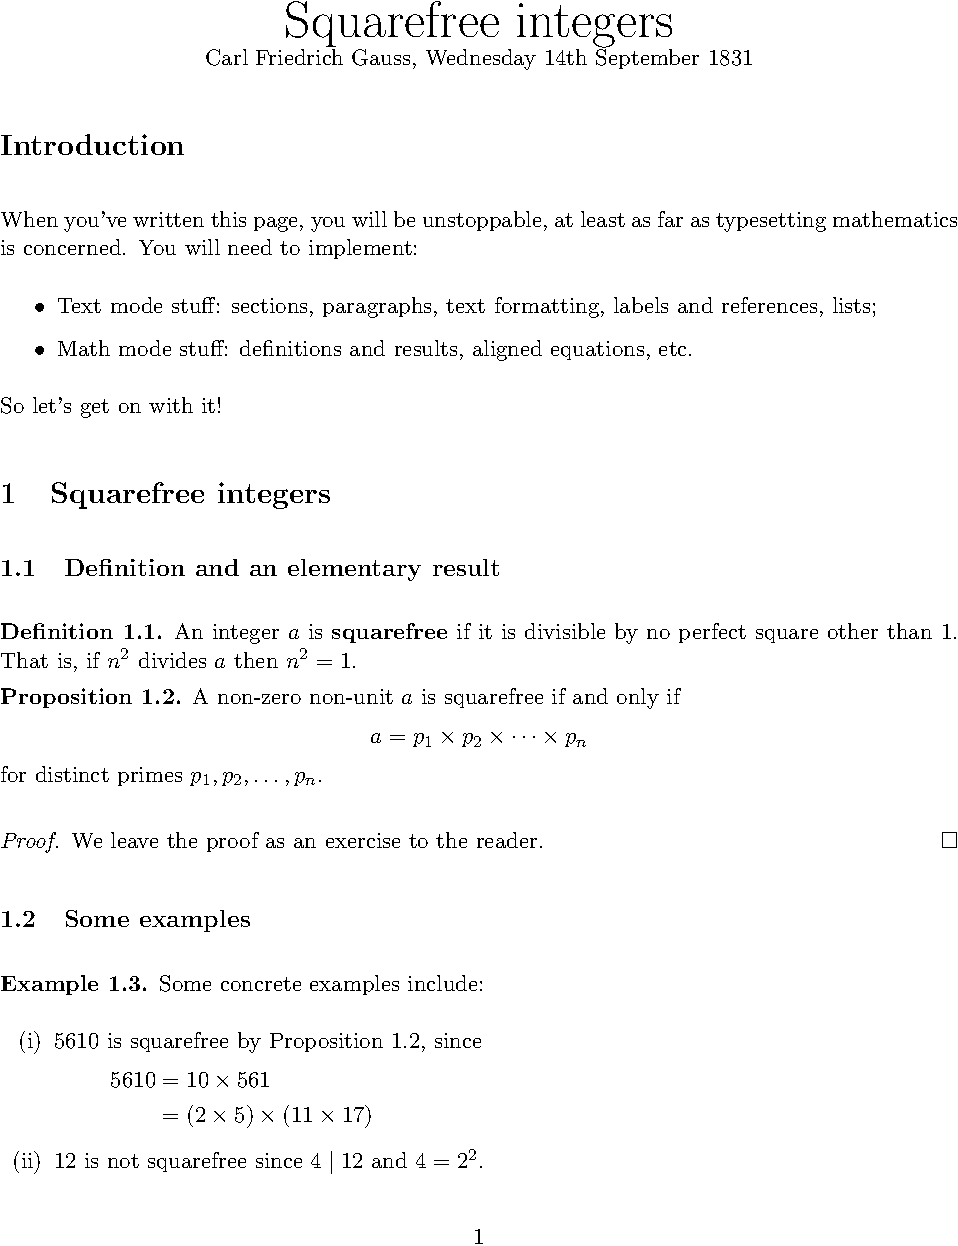
\includegraphics[keepaspectratio]{book/media/latex-exercise-crop.pdf}}}
\end{center}

\newpage
\subsection*{Template file}
\label{pTeXTemplate}

What follows is a template \texttt{.tex} file to get you started; it can be downloaded from \url{\bookurl/latex/}.

\lstinputlisting[basicstyle=\tt\scriptsize, xleftmargin=20pt, numbers=left]{book/media/template.tex}

\end{appendices}

\backmatter

{%
\part*{Indices}
\addcontentsline{toc}{part}{Indices}

\renewcommand{\chaptername}{Indices}
\newpage
\addcontentsline{toc}{chapter}{Index of topics}
\printindex

\addcontentsline{toc}{chapter}{Index of vocabulary}
\printindex[vocabulary]

\addcontentsline{toc}{chapter}{Index of notation}
\printindex[notation]

\addcontentsline{toc}{chapter}{Index of \LaTeX{} commands}
\printindex[latex]%
}

\clearpage\newpage\clearpage
\chapter*{Licence}
\pagestyle{empty}
\addcontentsline{toc}{part}{Licence}
    \renewcommand\chaptername{Licence}
    \chapter*{Licence}

\addcontentsline{toc}{part}{Licence}
\renewcommand\chaptername{Licence}

This book, in both physical and electronic form, is licensed under a Creative Commons Attribution-ShareAlike 4.0 International Public License. The licence is replicated below from the Creative Commons website:
\begin{center}
\url{https://creativecommons.org/licenses/by-sa/4.0/legalcode}
\end{center}
Please read the content of this licence carefully if you intend to share or adapt the material in this book.

If you have questions or would like to request permissions not granted by this licence, then contact the author (Clive Newstead, \url{\authoremail}).

\subsection*{Creative Commons Attribution-ShareAlike 4.0 International Public License}

{\small%
By exercising the Licensed Rights (defined below), You accept and agree to be bound by the terms and conditions of this Creative Commons Attribution-ShareAlike 4.0 International Public License (``Public License''). To the extent this Public License may be interpreted as a contract, You are granted the Licensed Rights in consideration of Your acceptance of these terms and conditions, and the Licensor grants You such rights in consideration of benefits the Licensor receives from making the Licensed Material available under these terms and conditions.

\subsection*{Section 1 --- Definitions.}

\begin{enumerate}[a.]
\item \textbf{Adapted Material} means material subject to Copyright and Similar Rights that is derived from or based upon the Licensed Material and in which the Licensed Material is translated, altered, arranged, transformed, or otherwise modified in a manner requiring permission under the Copyright and Similar Rights held by the Licensor. For purposes of this Public License, where the Licensed Material is a musical work, performance, or sound recording, Adapted Material is always produced where the Licensed Material is synched in timed relation with a moving image.
\item \textbf{Adapter's License} means the license You apply to Your Copyright and Similar Rights in Your contributions to Adapted Material in accordance with the terms and conditions of this Public License.
\item \textbf{BY-SA Compatible License} means a license listed at\\ \href{https://creativecommons.org/compatiblelicenses}{creativecommons.org/compatiblelicenses}, approved by Creative Commons as essentially the equivalent of this Public License.
\item \textbf{Copyright and Similar Rights} means copyright and/or similar rights closely related to copyright including, without limitation, performance, broadcast, sound recording, and Sui Generis Database Rights, without regard to how the rights are labeled or categorized. For purposes of this Public License, the rights specified in Section 2(b)(1)-(2) are not Copyright and Similar Rights.
\item \textbf{Effective Technological Measures} means those measures that, in the absence of proper authority, may not be circumvented under laws fulfilling obligations under Article 11 of the WIPO Copyright Treaty adopted on December 20, 1996, and/or similar international agreements.
\item \textbf{Exceptions and Limitations} means fair use, fair dealing, and/or any other exception or limitation to Copyright and Similar Rights that applies to Your use of the Licensed Material.
\item \textbf{License Elements} means the license attributes listed in the name of a Creative Commons Public License. The License Elements of this Public License are Attribution and ShareAlike.
\item \textbf{Licensed Material} means the artistic or literary work, database, or other material to which the Licensor applied this Public License.
\item \textbf{Licensed Rights} means the rights granted to You subject to the terms and conditions of this Public License, which are limited to all Copyright and Similar Rights that apply to Your use of the Licensed Material and that the Licensor has authority to license.
\item \textbf{Licensor} means the individual(s) or entity(ies) granting rights under this Public License.
\item \textbf{Share} means to provide material to the public by any means or process that requires permission under the Licensed Rights, such as reproduction, public display, public performance, distribution, dissemination, communication, or importation, and to make material available to the public including in ways that members of the public may access the material from a place and at a time individually chosen by them.
\item \textbf{Sui Generis Database Rights} means rights other than copyright resulting from Directive 96/9/EC of the European Parliament and of the Council of 11 March 1996 on the legal protection of databases, as amended and/or succeeded, as well as other essentially equivalent rights anywhere in the world.
\item \textbf{You} means the individual or entity exercising the Licensed Rights under this Public License. \textbf{Your} has a corresponding meaning.
\end{enumerate}

\subsection*{Section 2 -- Scope.}

\begin{enumerate}[a.]
\item \textbf{License grant.}

\begin{enumerate}[1.]
\item Subject to the terms and conditions of this Public License, the Licensor hereby grants You a worldwide, royalty-free, non-sublicensable, non-exclusive, irrevocable license to exercise the Licensed Rights in the Licensed Material to:
\begin{enumerate}[A.]
\item reproduce and Share the Licensed Material, in whole or in part; and
\item produce, reproduce, and Share Adapted Material.
\end{enumerate}
\item \underline{Exceptions and Limitations}. For the avoidance of doubt, where Exceptions and Limitations apply to Your use, this Public License does not apply, and You do not need to comply with its terms and conditions.
\item \underline{Term}. The term of this Public License is specified in Section 6(a).
\item \underline{Media and formats; technical modifications allowed}. The Licensor authorizes You to exercise the Licensed Rights in all media and formats whether now known or hereafter created, and to make technical modifications necessary to do so. The Licensor waives and/or agrees not to assert any right or authority to forbid You from making technical modifications necessary to exercise the Licensed Rights, including technical modifications necessary to circumvent Effective Technological Measures. For purposes of this Public License, simply making modifications authorized by this Section 2(a)(4) never produces Adapted Material.
\item \underline{Downstream recipients}.
\begin{enumerate}[A.]
\item \textit{\underline{Offer from the Licensor -- Licensed Material}. Every recipient of the Licensed Material automatically receives an offer from the Licensor to exercise the Licensed Rights under the terms and conditions of this Public License.}
\item \textit{\underline{Additional offer from the Licensor -- Adapted Material}. Every recipient of Adapted Material from You automatically receives an offer from the Licensor to exercise the Licensed Rights in the Adapted Material under the conditions of the Adapter’s License You apply.}
\item \textit{\underline{No downstream restrictions}. You may not offer or impose any additional or different terms or conditions on, or apply any Effective Technological Measures to, the Licensed Material if doing so restricts exercise of the Licensed Rights by any recipient of the Licensed Material.}
\end{enumerate}
\item \underline{No endorsement}. Nothing in this Public License constitutes or may be construed as permission to assert or imply that You are, or that Your use of the Licensed Material is, connected with, or sponsored, endorsed, or granted official status by, the Licensor or others designated to receive attribution as provided in Section 3(a)(1)(A)(i).
\end{enumerate}

\item \textbf{Other rights.}

\begin{enumerate}[1.]
\item Moral rights, such as the right of integrity, are not licensed under this Public License, nor are publicity, privacy, and/or other similar personality rights; however, to the extent possible, the Licensor waives and/or agrees not to assert any such rights held by the Licensor to the limited extent necessary to allow You to exercise the Licensed Rights, but not otherwise.
\item Patent and trademark rights are not licensed under this Public License.
\item To the extent possible, the Licensor waives any right to collect royalties from You for the exercise of the Licensed Rights, whether directly or through a collecting society under any voluntary or waivable statutory or compulsory licensing scheme. In all other cases the Licensor expressly reserves any right to collect such royalties.
\end{enumerate}
\end{enumerate}

\subsection*{Section 3 -- License Conditions.}

Your exercise of the Licensed Rights is expressly made subject to the following conditions.

\begin{enumerate}[a.]
\item \textbf{Attribution.}

\begin{enumerate}[1.]
\item If You Share the Licensed Material (including in modified form), You must:

\begin{enumerate}[A.]
\item retain the following if it is supplied by the Licensor with the Licensed Material:
identification of the creator(s) of the Licensed Material and any others designated to receive attribution, in any reasonable manner requested by the Licensor (including by pseudonym if designated);
a copyright notice;
\begin{enumerate}[i.]
\item a notice that refers to this Public License;
\item a notice that refers to the disclaimer of warranties;
\item a URI or hyperlink to the Licensed Material to the extent reasonably practicable;
\end{enumerate}

\item indicate if You modified the Licensed Material and retain an indication of any previous modifications; and
\item indicate the Licensed Material is licensed under this Public License, and include the text of, or the URI or hyperlink to, this Public License.
\end{enumerate}

\item You may satisfy the conditions in Section 3(a)(1) in any reasonable manner based on the medium, means, and context in which You Share the Licensed Material. For example, it may be reasonable to satisfy the conditions by providing a URI or hyperlink to a resource that includes the required information.

\item If requested by the Licensor, You must remove any of the information required by Section 3(a)(1)(A) to the extent reasonably practicable.
\end{enumerate}

\item \textbf{ShareAlike.}

In addition to the conditions in Section 3(a), if You Share Adapted Material You produce, the following conditions also apply.

\begin{enumerate}[1.]
\item The Adapter’s License You apply must be a Creative Commons license with the same License Elements, this version or later, or a BY-SA Compatible License.
\item You must include the text of, or the URI or hyperlink to, the Adapter's License You apply. You may satisfy this condition in any reasonable manner based on the medium, means, and context in which You Share Adapted Material.
\item You may not offer or impose any additional or different terms or conditions on, or apply any Effective Technological Measures to, Adapted Material that restrict exercise of the rights granted under the Adapter's License You apply.
\end{enumerate}
\end{enumerate}

\subsection*{Section 4 -- Sui Generis Database Rights.}

Where the Licensed Rights include Sui Generis Database Rights that apply to Your use of the Licensed Material:

\begin{enumerate}[a.]
\item for the avoidance of doubt, Section 2(a)(1) grants You the right to extract, reuse, reproduce, and Share all or a substantial portion of the contents of the database;
\item if You include all or a substantial portion of the database contents in a database in which You have Sui Generis Database Rights, then the database in which You have Sui Generis Database Rights (but not its individual contents) is Adapted Material, including for purposes of Section 3(b); and
\item You must comply with the conditions in Section 3(a) if You Share all or a substantial portion of the contents of the database.
\end{enumerate}

For the avoidance of doubt, this Section 4 supplements and does not replace Your obligations under this Public License where the Licensed Rights include other Copyright and Similar Rights.

\subsection*{Section 5 -- Disclaimer of Warranties and Limitation of Liability.}

\begin{enumerate}[a.]
{\bfseries
\item Unless otherwise separately undertaken by the Licensor, to the extent possible, the Licensor offers the Licensed Material as-is and as-available, and makes no representations or warranties of any kind concerning the Licensed Material, whether express, implied, statutory, or other. This includes, without limitation, warranties of title, merchantability, fitness for a particular purpose, non-infringement, absence of latent or other defects, accuracy, or the presence or absence of errors, whether or not known or discoverable. Where disclaimers of warranties are not allowed in full or in part, this disclaimer may not apply to You.
\item To the extent possible, in no event will the Licensor be liable to You on any legal theory (including, without limitation, negligence) or otherwise for any direct, special, indirect, incidental, consequential, punitive, exemplary, or other losses, costs, expenses, or damages arising out of this Public License or use of the Licensed Material, even if the Licensor has been advised of the possibility of such losses, costs, expenses, or damages. Where a limitation of liability is not allowed in full or in part, this limitation may not apply to You.%
}
\item The disclaimer of warranties and limitation of liability provided above shall be interpreted in a manner that, to the extent possible, most closely approximates an absolute disclaimer and waiver of all liability.
\end{enumerate}

\subsection*{Section 6 -- Term and Termination.}

\begin{enumerate}[a.]
\item This Public License applies for the term of the Copyright and Similar Rights licensed here. However, if You fail to comply with this Public License, then Your rights under this Public License terminate automatically.

\item Where Your right to use the Licensed Material has terminated under Section 6(a), it reinstates:

\begin{enumerate}[1.]
\item automatically as of the date the violation is cured, provided it is cured within 30 days of Your discovery of the violation; or
\item upon express reinstatement by the Licensor.
\end{enumerate}

For the avoidance of doubt, this Section 6(b) does not affect any right the Licensor may have to seek remedies for Your violations of this Public License.

\item For the avoidance of doubt, the Licensor may also offer the Licensed Material under separate terms or conditions or stop distributing the Licensed Material at any time; however, doing so will not terminate this Public License.

\item Sections 1, 5, 6, 7, and 8 survive termination of this Public License.
\end{enumerate}

\subsection*{Section 7 -- Other Terms and Conditions.}

\begin{enumerate}[a.]
\item The Licensor shall not be bound by any additional or different terms or conditions communicated by You unless expressly agreed.
\item Any arrangements, understandings, or agreements regarding the Licensed Material not stated herein are separate from and independent of the terms and conditions of this Public License.
\end{enumerate}

\subsection*{Section 8 -- Interpretation.}

\begin{enumerate}[a.]
\item For the avoidance of doubt, this Public License does not, and shall not be interpreted to, reduce, limit, restrict, or impose conditions on any use of the Licensed Material that could lawfully be made without permission under this Public License.
\item To the extent possible, if any provision of this Public License is deemed unenforceable, it shall be automatically reformed to the minimum extent necessary to make it enforceable. If the provision cannot be reformed, it shall be severed from this Public License without affecting the enforceability of the remaining terms and conditions.
\item No term or condition of this Public License will be waived and no failure to comply consented to unless expressly agreed to by the Licensor.
\item Nothing in this Public License constitutes or may be interpreted as a limitation upon, or waiver of, any privileges and immunities that apply to the Licensor or You, including from the legal processes of any jurisdiction or authority.
\end{enumerate}
}

\end{document}